\documentclass[12pt,letterpaper]{book}
\usepackage[margin=0.9in]{geometry}
\usepackage[utf8]{inputenc} 
\usepackage[english]{babel}
\usepackage{graphicx}
\usepackage{amsmath, amsfonts, amssymb, amsthm, thmtools}
\usepackage{braket} 
\usepackage{relsize} 
\usepackage{float}
\usepackage{mathtools}
\usepackage{lmodern} 
\usepackage[T1]{fontenc}
\usepackage{fancyhdr}
\usepackage[dvipsnames]{xcolor} % Colors, use dvipsnames for more color options
\usepackage{framed} % Fancy leftbar
\usepackage[normalem]{ulem}
\usepackage{tikz-cd} % Diagrams
\usepackage{tikz} % General purpose graphics
\usepackage{tikz-3dplot}
\usepackage[most]{tcolorbox} % For theorem boxing
\usepackage{bm} % For better bold math font
\usepackage{old-arrows} 
\usepackage[usestackEOL]{stackengine}
\usepackage{sectsty}
\usepackage[hyperfootnotes=false]{hyperref} % For clickable table of contents
\usepackage[linesnumbered, ruled, boxruled]{algorithm2e} % Fancy algorithm presentation
\usepackage{calc} % For simpler calculation - used for spacing the index letter headings correctly
\usepackage{makeidx} % Required to make an index
\usepackage{verbatim}
\usepackage{titlesec} % Allows customization of titles
\usepackage{enumitem} % Customize lists
\usepackage{booktabs} %  Required for nicer horizontal rules in tables
\usepackage{eso-pic} %  Required for specifying an image background in the title page
\usepackage{titletoc, tocloft, pgffor}
\usepackage[titletoc]{appendix} % For appendix
\usepackage{braids}
\usepackage{adjustbox} % Very useful boxing environment
\usepackage{setspace} % Variable line spacing
\usepackage{soul}

%----------------------------------------------------------------------------------------
%	Global Document Settings
%----------------------------------------------------------------------------------------
\setcounter{section}{1} % Avoid counting from zero
\linespread{1.1} % Set line spacing
\graphicspath{{pictures/}}% Set graphics directory
\hypersetup{ % Set hyperref settings
    colorlinks,
    citecolor=black,
    filecolor=black,
    linkcolor=black,
    urlcolor=black
}
\setitemize{noitemsep,topsep=0.5em, parsep=0.5em ,partopsep=0pt}
\setlist{nolistsep} %  Reduce spacing between bullet points and numbered lists

%----------------------------------------------------------------------------------------
%	TikZ Settings
%----------------------------------------------------------------------------------------
\usetikzlibrary{
    arrows, 
    arrows.meta, 
    braids, 
    calc, 
    shapes.geometric,
    decorations.markings,
    decorations.pathreplacing, 
    intersections,
    hobby
}
% Set stealth arrows in TikzCD
\tikzcdset{
    arrow style = tikz, diagrams={>={Stealth[scale=1]}}
} 
% Set stealth arrows in TikZ
\tikzset{
    >={Stealth[scale=1]}
} 

%----------------------------------------------------------------------------------------
%	Math Commands
%----------------------------------------------------------------------------------------
% First we need to overwrite some existing commands. 
\let\*\relax 
\let\path\relax 
\let\ker\relax 
\let\im\relax
\let\hom\relax
\let\Set\relax
\let\top\relax
\let\ll\relax
%% Various Math Operators
\DeclareMathOperator{\im}{\rm{Im}}
\DeclareMathOperator{\id}{\mathrm{id}}
\DeclareMathOperator{\ob}{\mathrm{Ob}}
\DeclareMathOperator{\*}{ \mathbin{*} }
\DeclareMathOperator{\path}{\mathrm{Path}} 
\DeclareMathOperator{\nat}{\mathrm{Nat}}
\DeclareMathOperator{\dom}{\mathrm{Dom}}
\DeclareMathOperator{\cod}{\mathrm{Cod}}
\DeclareMathOperator{\gal}{\mathrm{Gal}}
\DeclareMathOperator{\aut}{\mathrm{Aut}}
\DeclareMathOperator{\cone}{\mathrm{Cone}}
\DeclareMathOperator{\fun}{\mathrm{Fun}}
\DeclareMathOperator{\proj}{\mathrm{proj}}
\DeclareMathOperator{\coker}{\mathrm{Coker}}
\DeclareMathOperator{\aend}{\mathrm{End}} %a is added because LaTeX does not allow commands to begin with "end."
\DeclareMathOperator{\spec}{\mathrm{Spec}}
\DeclareMathOperator{\ker}{\mathrm{Ker}}
\DeclareMathOperator*{\Lim}{\mathrm{Lim }}
\DeclareMathOperator*{\Colim}{\mathrm{Colim }}
\DeclareMathOperator{\hom}{\mathrm{Hom}}
\DeclareMathOperator{\Char}{\mathrm{char}} % We'd prefer \char, but... NEVER overwrite \char! TeX will die.
\DeclareMathOperator{\ll}{\mathcal{L}}

%% General Math Shortcuts
\newcommand{\zz}{\mathbb{Z}}
\newcommand{\rr}{\mathbb{R}}
\newcommand{\nn}{\mathbb{N}}
\newcommand{\qq}{\mathbb{Q}}
\newcommand{\normal}{\unlhd}
\newcommand{\join}{\vee}
\newcommand{\meet}{\wedge}
\renewcommand{\epsilon}{\varepsilon}
\renewcommand{\phi}{\varphi}
\renewcommand{\subset}{\subseteq}
\newcommand{\op}{^{\mathrm{op}}}

%% Category Shortcuts
\newcommand{\bb}{\mathcal{B}}
\newcommand{\cc}{\mathcal{C}}
\newcommand{\dd}{\mathcal{D}}
\newcommand{\ee}{\mathcal{E}}
\newcommand{\ff}{\mathcal{F}}
\newcommand{\mm}{\mathcal{M}}
\newcommand{\pp}{\mathcal{P}} 
\newcommand{\qqq}{\mathcal{Q}}
\newcommand{\vv}{\mathcal{V}}
\newcommand{\ww}{\mathcal{W}}
\renewcommand{\aa}{\mathcal{A}}
\renewcommand{\ee}{\mathcal{E}}
\renewcommand{\ss}{\mathcal{S}}
\renewcommand{\wp}{\mathcal{W}_{\mathrm{P}}}

% Category of Sets
\DeclareMathOperator{\Set}{\mathbf{Set}}
\DeclareMathOperator{\finset}{\mathbf{FinSet}}
\DeclareMathOperator{\finord}{\mathbf{FinOrd}}
% "Algebraic" categories
\DeclareMathOperator{\grp}{\mathbf{Grp}}
\DeclareMathOperator{\ab}{\mathbf{Ab}}
\DeclareMathOperator{\ring}{\mathbf{Ring}}
\DeclareMathOperator{\cring}{\mathbf{CRing}}
\DeclareMathOperator{\mon}{\mathbf{Mon}}
\DeclareMathOperator{\rmod}{\mathbf{-Mod}}
\DeclareMathOperator{\alg}{\mathbf{Alg}}
\DeclareMathOperator{\fld}{\mathbf{Fld}}
% Other Categories
\DeclareMathOperator{\open}{\mathbf{Open}}
\DeclareMathOperator{\top}{\mathbf{Top}}
\DeclareMathOperator{\Toph}{\mathbf{Toph}}
\DeclareMathOperator{\vect}{\mathbf{Vect}}
\DeclareMathOperator{\cat}{\mathbf{Cat}}

% A nice \to command
\renewcommand{\to}{\mathbin{\tikz[baseline] \draw[-{Stealth[length=5pt,width=4pt]}] (0pt,.6ex) -- (3.5ex,.6ex);}} 

% A nice isomorphism arrow
\newcommand{\isomarrow}{\mathrel{\setstackgap{S}{-0.5pt}\ensurestackMath{\Shortstack{\scriptstyle\sim\\ \longrightarrow}}}} 

% A nice \cdot symbol, which is bigger than \cdot but smaller than \bullet. 
\makeatletter % So that we access commands with "@" in them
\newcommand*\bcdot{\mathpalette\bcdot@{.6}}
\newcommand*\bcdot@[2]{\mathbin{\vcenter{\hbox{\scalebox{#2}{$\m@th#1\bullet$}}}}}
\DeclareMathOperator{\bigcdot}{\mathbin{\bcdot}}
\makeatother

% These are \Lim and \Colim with arrows underneath
\newcommand{\Arrowto}[1]{\parbox{#1}{\tikz{\draw[->](0,0)--(#1,0);}}}
\newcommand{\Arrowfrom}[1]{\parbox{#1}{\tikz{\draw[<-](0,0)--(#1,0);}}}
\DeclareMathOperator*{\Limto}{\Lim_{\Arrowto{0.8cm}}}
\DeclareMathOperator*{\Limfrom}{\Lim_{\Arrowfrom{0.8cm}}}
\DeclareMathOperator*{\Colimto}{\Colim_{\Arrowto{1cm}}}
\DeclareMathOperator*{\Colimfrom}{\Colim_{\Arrowfrom{1cm}}}

% To type out adjunctions
\newcommand{\adjunction}[4]{
    \begin{tikzcd}[ampersand replacement = \&] %\newcommand freaks out with & symbols
        #1
        \arrow[r, shift right = -0.5ex, "#2"]
        \&
        #3
        \arrow[l, shift right = -0.5ex, "#4"]
    \end{tikzcd}
}

%----------------------------------------------------------------------------------------
%	Non-Math Commands
%----------------------------------------------------------------------------------------

% Some colors
\definecolor{processBlue}{HTML}{E0F8FF}
\definecolor{mypurple}{HTML}{4D34A4}
\definecolor{navy}{RGB}{20,150,220}
\definecolor{purp}{HTML}{CDCBFF}

% For enumerate environment
\renewcommand{\labelenumi}{{\bf (\alph{enumi})}} 

% To easily reference universal morphism definition
\newcommand{\universalDToF}[1]{\hyperref[definition:universal_morphism_from_D_to_F]{\textcolor{blue}{#1}}}
\newcommand{\universalFToD}[1]{\hyperref[definition:universal_morphism_from_F_to_D]{\textcolor{blue}{#1}}}

\renewcommand{\cftpartfont}{\normalsize}% To adjust contents fontsize
\renewcommand{\thealgocf}{} %removes annoying numbering in algorithm header

%----------------------------------------------------------------------------------------
%	Theorem Environments
%----------------------------------------------------------------------------------------

\input{latex_commands} % Proof, Example, Remark, Important Statement Environments

% Custom Theorem to override numbering
\newtheorem{innercustomthm}{Theorem}
\newenvironment{customthm}[1]
{\renewcommand\theinnercustomthm{#1}\innercustomthm}
{\endinnercustomthm}

% Custom Proposition to override numbering
\newtheorem{innercustomprop}{Proposition}
\newenvironment{customprop}[1]
{\renewcommand\theinnercustomprop{#1}\innercustomprop}
{\endinnercustomprop}

% Custom Lemma to override numbering
\newtheorem{innercustomlemma}{Lemma}
\newenvironment{customlemma}[1]
{\renewcommand\theinnercustomlemma{#1}\innercustomlemma}
{\endinnercustomlemma}

% Theorem customization and colorings
\theoremstyle{definition}
\declaretheoremstyle[spacebelow=6pt, headfont=\color{RoyalPurple}\normalfont\bfseries]{Defn}
\declaretheoremstyle[spacebelow=6pt, headfont=\color{RoyalBlue}\normalfont\bfseries]{Prop}

% Theorem 
\newtheorem{theorem}{Theorem}[section]

% Definition, Proposition, Corollary, Lemma
\declaretheorem[name=Definition, style=Defn, sibling=theorem]{definition}
\declaretheorem[name=Proposition, style=Prop, sibling=theorem]{proposition}
\declaretheorem[name=Corollary, style=Prop, sibling=theorem]{corollary}
\declaretheorem[name=Lemma, style=Prop,sibling=theorem]{lemma}

%----------------------------------------------------------------------------------------
%	Front Cover, Chapter, and Page Designs
%----------------------------------------------------------------------------------------

% Background Image
\newcommand{\BackgroundPic}{
    \put(0,0){%
    \parbox[b][\paperheight]{\paperwidth}{%
    \vfill
    \centering 
    \includegraphics[width=\paperwidth,height=\paperheight]{mountain.jpeg}%
    \vfill
}}}

% Front Cover
\newcommand{\frontCover}{
    \AddToShipoutPicture*{\BackgroundPic} 
    \section*{\textcolor{White}{Category Theory}}  
    \vspace{20cm}

    {\large \textcolor{White}{Luke Trujillo}}
    \newpage
    \tableofcontents
}

% Header design
\pagestyle{fancy}
\renewcommand{\chaptermark}[1]{\markboth{\sffamily\normalsize\bfseries\chaptername\ \thechapter.\ #1}{}} % Chapter text font settings
\renewcommand{\sectionmark}[1]{\markright{\sffamily\normalsize\thesection\hspace{5pt}#1}{}} % Section text font settings
\fancyhf{} 
\fancyhead[LE,RO]{\sffamily\normalsize\thepage} % Font setting for the page number in the header
\fancyhead[LO]{\rightmark} % Print the nearest section name on the left side of odd pages
\fancyhead[RE]{\leftmark} % Print the current chapter name on the right side of even pages
\renewcommand{\headrulewidth}{0.5pt} % Width of the rule under the header
\addtolength{\headheight}{2.5pt} % Increase the spacing around the header slightly
\renewcommand{\footrulewidth}{0pt} % Removes the rule in the footer
\fancypagestyle{plain}{\fancyhead{}\renewcommand{\headrulewidth}{0pt}} % Style for when a plain pagestyle is specified

% Chapter design
% The canonical, moronic way to store values because TeX is moronic 
\newcommand{\thechapterimage}{}
\newcommand{\chapterimage}[1]{\renewcommand{\thechapterimage}{#1}}
% Numbered chapters with mini tableofcontents
\makeatletter % Need to access commands with @
\def\thechapter{\arabic{chapter}}
\def\@makechapterhead#1{ 
{\centering \normalfont\sffamily
\ifnum \c@secnumdepth >\m@ne
\if@mainmatter
\startcontents
\begin{tikzpicture}[remember picture,overlay]
    \node at (current page.north west) {
        \begin{tikzpicture}[remember picture,overlay]
            \node[anchor=north west,inner sep=0pt] at (0,0) {
                \includegraphics[width=\paperwidth]{\thechapterimage}
            };
            \draw[anchor=west] (1cm,-9cm) 
                node [rounded corners=20pt,
                    fill=ProcessBlue!10!white,
                    text opacity=1,
                    draw=NavyBlue,
                    draw opacity=1,
                    line width=1.5pt,
                    fill opacity=.6,inner sep=12pt]
                    {
                        \huge\rmfamily\bfseries\textcolor{black}{\thechapter. \LARGE#1\strut\makebox[22cm]{}}
                    }; % Controls outside border
        \end{tikzpicture}
        };
\end{tikzpicture}}
\par\vspace*{230\p@}
\fi
\fi}
\makeatother

% Section number design 
\titleformat{\section}[hang]{\bfseries}{
\hspace{-1.6cm} % align square and number outside the margin
\begin{minipage}{0.1\textwidth}
    \vspace{-0.15cm}
    \begin{tikzpicture}
        \filldraw[thick, navy, opacity=0.6] (-0.1,-0.1)--(1.1,-0.1)--(1.1,1.1)--(-0.1,1.1)--cycle;
        \node at (0.65, 0.5) {\Large\bfseries{\color{white}\thesection}\enspace};
    \end{tikzpicture}
\end{minipage}
}{1pt}{\Large\bfseries\filright}

%----------------------------------------------------------------------------------------
%	\begin{document}
%----------------------------------------------------------------------------------------

\begin{document} 

    \frontCover

    \begin{spacing}{1}
\linespread{1}



\newpage
\section*{Acknowledgments}
I want to thank Professor Dagan Karp at Harvey Mudd College, my undergraduate adviser, for being an amazing 
mentor and for providing me extremely helpful advice and support during my time at Harvey Mudd.
Professor Karp also supervised an independent study for which a large portion of this text originated from.

I also want to thank Professor Vin de Silva at Pomona College, my undergraduate thesis adviser.
Through Professor de Silva's humility and patience I learned a great deal of category theory and many tecniques
how to write mathematics clearly. I also would have never produced Section \ref{section:coherence_theorem}
or the chapter on Persistence Modules without his feedback.

I'd also like to thank Daniel Donnelley Jr for catching dozens of typos and 
statements that were plain wrong; errors that could only have been caught 
through a thorough reading. Donnelley also offered extremely helpful feedback, and
suggested many sentence revisions and section restructurings which were all 
in the best interest of increasing the readability of this text.  

\section*{About the Cover}
The cover of the text is a long exposure shot I took from a popular 
hiking trail on top of Mount Baldy in Claremont, CA. You can probably 
tell neither the camera nor the photographer were very good, and that there's a lot 
of light pollution in Southern California. 


\newpage
{\centering \huge\textbf{Warning!}}
\\
\\

This is a work in progress, and there are lots of typos. Some sections 
are being reorganized. I probably won't be ``finished'' for a long time.
\texttt{ltrujillo@hmc.edu} .


\end{spacing}
 

    \chapterimage{chapter1_pic/functors.pdf} % Chapter heading image
    \chapter{Categories, Functors and Natural Transformations.} 
    \section{Introduction: What are the Foundations of Math?} 
    Category theory attempts to ``zoom out'' of mathematical constructions
    and to point out the higher level relationships between different mathematical
    constructions. The three main concepts are categories, functors, and
    natural transformations, although the theory grew out of
    implications of these main concepts. 
    
    
    These main concepts were first seen in the study of algebraic
    topology, since 
    it was observed that topological problems could be reduced to
    algebraic, and vice versa. But how? Since there was no formal
    notion for what it really meant to take a topological space $X$
    and associate it with some group $\pi(X)$, 
    category theory came about to formalize this. 

    However, as we shall soon see, category theory has a big problem. 
    Specifically, there isn't a universally agreed upon foundation for
    category theory, or for mathematics in general. 
    \begin{center}
        \textbf{What do we mean by foundations?}
    \end{center}
    Well, consider a topological space $X$, or a group $G$, or a
    domain $\mathbb{R}$. Then suppose I ask you
    ``What is $X$?'' or ``What is $G$'' or ``What is $\mathbb{R}$?'' 
    Well, you'll tell me it's a topological space, a
    group, or the set of real numbers and
    list the axioms for each object. 

    That is, a correct answer will characterize $X$, $G$ or $\mathbb{R}$ as a
    set which satisfies 
    some axioms. But really, that's what all our mathematical objects
    are. So at this point, our foundations \textbf{are grounded in set
    theory.}

    \begin{center}
        \textbf{What is set theory?}
    \end{center}
    Suppose I ask you what is set theory. While we all know there are 
    different set theories, most people don't think about set theory axioms on a daily 
    and won't know (like myself). But answering
    this question requires answering the next. 

    \begin{center}
    \textbf{What is a set?}
    \end{center}
    We usually never have to face this question. But in developing a
    theory that considers relationships between different sets, we
    have to. 
    
    Our intuition tells us that sets $X$ are a \textbf{collection of
    objects, and that every collection of objects is a set}. We
    intuitively \textit{think} that  
    we can form collections of objects to create a set $X$, and that
    we can form 
    intersection and unions between sets, or even compute power
    sets, to produce other sets. We also \textit{think} we can also form sets such as 
    \[
        X = \{x \mid \phi(x) \}
    \]
    where $\phi$ is some logical condition of inclusion. However, this
    leads to paradoxes, one of the most famous known as Russel's
    Paradox which we can describe as follows. 

    \noindent\textbf{Russel's Paradox.}
    Let $X$ be a set such that 
    \[
        X = \{A \text{ is a set }\mid A \text{ is not a member of itself.}\}
    \]
    
    Now observe the following. 
    \begin{itemize}
        \item[1.] If $X \in X$, then consequently $X$ is not a member
        of itself. In other words, if $X \in X$, then $X \not\in X$.

        Clearly, this is a contradiction. Since $X \in X$ is nonsense,
        $X \not\in X$, right? 

        \item[2.] Suppose $X \not\in X$. Then $X$ is not a member of
        itself, so $X \in X$ by the condition of member of $X$. In
        other words, $X \not\in X \implies X \in X$.
    \end{itemize}
    See the problem here? \textbf{Not every collection of objects is a
    set.} So our previous notions of sets aren't correct.

    \textcolor{MidnightBlue}{Note that our trouble arose when we said
    that \textbf{a set is a collection of objects, and a collection of
    objects is a set.} 
    This is because no, not every collection of objects is a set.
    Thus we need to go back and fix our definition of a set.
    }

    \begin{center}
        \textbf{What do we do?}
    \end{center}
    This is what many mathematicians asked in the early 1900s
    when they identified the paradoxes that arise from our notion of
    a set. The result has been multiple different types of set theories, 
    and so there isn't a clear 
    choice on what to make our foundations. However, this isn't a huge problem 
    for category theory. Category theory 
    has its own core axioms, but the fact that there are different set theories 
    simply means that such core axioms will be phrased differently under different 
    set theories (although there are some cases where 
    one does need to be careful with their foundations).
    In this text, we'll be a bit sloppy with the foundations of category theory, 
    although  we will point out where we need to be careful.


    \newpage
    \section{Motivation for Category Theory}
    What do groups $G$, topological spaces $X$ and vector spaces $V$ have 
    in common?
    \emph{We use different letters to describe them!} Seriously, that is one major 
    difference. Why? Because our brains are organizational and thrive off of associations, 
    e.g., $G$ with group, $X$ with topological spaces, etc. This is great 
    for thinking, but the mental separation of these constructions hides a bigger 
    picture.

    Let's look at what these things look like. 
    With groups, we are often mapping between groups via group homomorphisms.
    For example, below we have the chain complex of abelian groups with boundary 
    operator $\partial_n: C_n \to C_{n-1}$, with the familiar property that
    $\partial_n \circ \partial_{n-1} = 0$.
    \begin{center}
    \adjustbox{scale = 0.85}{
        \tikzstyle{A} = [fill=ProcessBlue!20]
        \tikzstyle{B} = [fill=ProcessBlue!30]
        \tikzstyle{C} = [fill=ProcessBlue!40]
        \begin{tikzpicture}[>=stealth]
            \pgfmathsetmacro{\height}{2.5}
            \pgfmathsetmacro{\heightstep}{0.5}
            \pgfmathsetmacro{\width}{2}
            \pgfmathsetmacro{\widthstep}{0.5}
            
            \pgfmathsetmacro{\Ax}{\height}
            \pgfmathsetmacro{\Ay}{\width}
            \pgfmathsetmacro{\Bx}{\height - \heightstep}
            \pgfmathsetmacro{\By}{\width - \widthstep}
            \pgfmathsetmacro{\Cx}{\height - \heightstep -\heightstep}
            \pgfmathsetmacro{\Cy}{\width - \widthstep - \widthstep}
    
            \begin{scope}
                % draws the three ellipses
                \filldraw[A] (0,0) ellipse (\Ay cm and \Ax cm);
                \draw (0,0) ellipse (\Ay cm and \Ax cm);
    
                \filldraw[B] (0,-\heightstep) ellipse (\By cm and \Bx cm);
                \draw (0,-\heightstep) ellipse (\By cm and \Bx cm);
    
                \filldraw[C] (0,-\heightstep - \heightstep) ellipse (\Cy cm and \Cx cm);
                \draw (0,-\heightstep - \heightstep) ellipse (\Cy cm and \Cx cm);
    
                % labels the ellipses
                \node at (0, \height - 0.3) {$C_n$};
                \node at (0, \height - 1.3) {$Z_n$};
                \node at (0, \height - 2.4) {$B_n$};
            \end{scope}
    
            \begin{scope}[xshift = 5cm]
                % draws the three ellipses
                \filldraw[A] (0,0) ellipse (\Ay cm and \Ax cm);
                \draw (0,0) ellipse (\Ay cm and \Ax cm);
        
                \filldraw[B] (0,-\heightstep) ellipse (\By cm and \Bx cm);
                \draw (0,-\heightstep) ellipse (\By cm and \Bx cm);
        
                \filldraw[C] (0,-\heightstep - \heightstep) ellipse (\Cy cm and \Cx cm);
                \draw (0,-\heightstep - \heightstep) ellipse (\Cy cm and \Cx cm);
    
                % labels the ellipses
                \node at (0, \height - 0.3) {$C_{n-1}$};
                \node at (0, \height - 1.3) {$Z_{n-1}$};
                \node at (0, \height - 2.4) {$B_{n-1}$};
            \end{scope}
    
            \begin{scope}[xshift = 10cm]
                % draws the three ellipses
                \filldraw[A] (0,0) ellipse (\Ay cm and \Ax cm);
                \draw (0,0) ellipse (\Ay cm and \Ax cm);
        
                \filldraw[B] (0,-\heightstep) ellipse (\By cm and \Bx cm);
                \draw (0,-\heightstep) ellipse (\By cm and \Bx cm);
        
                \filldraw[C] (0,-\heightstep - \heightstep) ellipse (\Cy cm and \Cx cm);
                \draw (0,-\heightstep - \heightstep) ellipse (\Cy cm and \Cx cm);
    
                % labels the ellipses
                \node at (0, \height - 0.3) {$C_{n-2}$};
                \node at (0, \height - 1.3) {$Z_{n-2}$};
                \node at (0, \height - 2.4) {$B_{n-2}$};
            \end{scope}
    
            % draws the arrows
            \draw[->] (0.5, \height-0.5) -- (4.2cm, \height-2.5) node[midway, above] {$\partial_n$};
            \draw[->] (0.5+5.5cm, \height-0.5) -- (4.2cm+5cm, \height-2.5) node[midway, above] {$\partial_{n-1}$};
    
            \draw[->] (0.2, \height-1.6) -- (4.8, -2.3)node[midway, below] {$\partial_n$};
            \draw[->] (0.2+5.5cm, \height-1.6) -- (9.7cm, -2.3)node[midway, below] {$\partial_{n-1}$};
    
            \filldraw (0,-2.5) circle (0.5mm) node[below] {$0$};
            \filldraw (5cm,-2.5) circle (0.5mm) node[below] {$0$};
            \filldraw (10cm,-2.5) circle (0.5mm) node[below] {$0$};
    
            \node at (-3cm, 0cm) {$\cdots$};
            \node at (13cm, 0cm) {$\cdots$};
        \end{tikzpicture}
    }

    \emph{A chain complex; the image of $\partial_n$ is $B_{n-1}$, while the kernel 
    of $\partial_n$ is $Z_{n}$.}
    \end{center}

    Within topology, we are often mapping topological spaces via continuous functions.
    \begin{center}
        % controls surface color
        \tikzstyle{surface}=[left color=NavyBlue!30,right color=NavyBlue!60, 
        opacity = 0.8
        ]
        % controls the embedded triangle surface color
        \tikzstyle{em_triangle}=[left color=Purple!30,right color=Purple!60,
        opacity = 0.8
        ]
        % controls the triangle surface color
        \tikzstyle{triangle}=[left color=Purple!30,right color=Purple!50,
        opacity = 0.8
        ]
        % controls the shadow coloring
        \tikzstyle{shadow}=[left color=gray!10,right color=gray!20, opacity = 0.8, rounded corners=0.5cm]
    
        \begin{tikzpicture}[>=stealth]
            \pgfmathsetmacro{\scale}{4}
            \pgfmathsetmacro{\zoffset}{-10}
            \pgfmathsetmacro{\yoffset}{-3}
            \pgfmathsetmacro{\xoffset}{-6}
        
            % the origin
            \coordinate (origin) at (-\xoffset, -\yoffset, -\zoffset);
        
            % the axes
            \coordinate (A) at (\scale -\xoffset, -\yoffset,-\zoffset);
            \coordinate (B) at (-\xoffset, \scale-\yoffset,-\zoffset);
            \coordinate (C) at (-\xoffset, -\yoffset,\scale-\zoffset);
        
            \draw[semithick, ->] (origin) --  (A);
            \draw[semithick, ->] (origin) --  (B);
            \draw[semithick, ->] (origin) --  (C);
    
            % the leftmost axes 
            \pgfmathsetmacro{\axesshift}{8}
            \coordinate (a) at (\scale -\xoffset - \axesshift, -\yoffset,-\zoffset);
            \coordinate (b) at (-\xoffset -  \axesshift, \scale-\yoffset,-\zoffset);
            \coordinate (c) at (-\xoffset - \axesshift, -\yoffset,\scale-\zoffset);
            
            % the leftmost origin
            \coordinate (left_origin) at (-\xoffset - \axesshift, -\yoffset, -\zoffset);
            \draw[semithick, ->] (left_origin) --  (a);
            \draw[semithick, ->] (left_origin) --  (b);
            \draw[semithick, ->] (left_origin) --  (c);
    
            % triangle
            \pgfmathsetmacro{\trianglelength}{2.5}
    
            % boundary of triangle
            \draw (\trianglelength-\xoffset - \axesshift,-\yoffset,-\zoffset) 
            -- 
            (-\xoffset -\axesshift, \trianglelength-\yoffset, -\zoffset) 
            -- 
            (-\xoffset -\axesshift, -\yoffset, \trianglelength-\zoffset) -- cycle;
    
            % interior of triangle
            \shade[triangle]
            (\trianglelength-\xoffset - \axesshift,-\yoffset,-\zoffset) 
            -- 
            (-\xoffset -\axesshift, \trianglelength-\yoffset, -\zoffset) 
            -- 
            (-\xoffset -\axesshift, -\yoffset, \trianglelength-\zoffset) -- cycle;
    
            
            % the arrow
            \draw[->] ([xshift = -2cm, yshift = 1.5cm]a) 
            to[bend left] 
            ([xshift= 0.5cm, yshift = 4cm]C);
            \node at ([xshift = 0.5cm, yshift = 3.1cm]a) {$f$};
    
            % number of lines (n x n grid)
            \pgfmathsetmacro{\nlines}{22}
            % coordinates
            \coordinate (A) at (0,0);
            \path (A);\pgfgetlastxy{\ax}{\ay} 
            \coordinate (B) at (3,-2);
            \path (B);\pgfgetlastxy{\bx}{\by}
            \coordinate (C) at (8,0);
            \path (C);\pgfgetlastxy{\cx}{\cy}
            \coordinate (D) at (5, 2);
            \path (D);\pgfgetlastxy{\dx}{\dy}
        
            %incoming angles
            \pgfmathsetmacro{\ABout}{-5}
            \pgfmathsetmacro{\ABin}{150}
            
            \pgfmathsetmacro{\BCout}{-5}
            \pgfmathsetmacro{\BCin}{150}
        
            \pgfmathsetmacro{\CDout}{150}
            \pgfmathsetmacro{\CDin}{-10}
            
            \pgfmathsetmacro{\DAout}{150}
            \pgfmathsetmacro{\DAin}{-10}
        
            % draws the shadow underneath
            \shade[shadow]
            ([xshift = 1cm, yshift = -2cm]A)
            --
            ([xshift = 0cm, yshift = -2cm]B) 
            --
            ([xshift = -1cm, yshift = -2cm]C)
            --
            ([xshift = 0cm, yshift = -2.7cm]D) 
            --
            % to[out=\DAout,in=\DAin]  
            cycle;
        
            % draws the colored surface 
            \shade[surface] 
            (A)
            to[out=\ABout,in=\ABin] 
            (B) 
            to[out=\BCout,in=\BCin] 
            (C)
            to[out=\CDout,in=\CDin] 
            (D) 
            to[out=\DAout,in=\DAin]  cycle;
        
            % draws the thin boundary
            \draw[line width = 0.05mm]
            (A)
            to[out=\ABout,in=\ABin] 
            (B) 
            to[out=\BCout,in=\BCin] 
            (C)
            to[out=\CDout,in=\CDin] 
            (D) to[out=155,in=\DAin] cycle;
        
            % draws the vertical grid lines
            \foreach \n in {1,2, ..., \nlines}{
                \pgfmathsetmacro{\step}{\n/\nlines}
                \path (A) to[out=\ABout,in=\ABin] coordinate[pos=\step] (A\n) (B);
                \path (B) to[out=\BCout,in=\BCin] coordinate[pos=\step] (B\n) (C);
                \path (D) to[in=\CDout,out=\CDin] coordinate[pos=\step] (C\n) (C);
                \path (A) to[in=\DAout,out=\DAin] coordinate[pos=\step] (D\n) (D);
            }
        
            % draws the horizontal grid lines
            \foreach \n in {1,2,...,\nlines}{
                \path (A\n); \pgfgetlastxy{\ax\n}{\ay\n} 
                \path (B\n); \pgfgetlastxy{\bx\n}{\by\n} 
                \path (C\n); \pgfgetlastxy{\cx\n}{\cy\n} 
                \path (D\n); \pgfgetlastxy{\dx\n}{\dy\n} 
                \draw[line width = 0.05mm]
                (\bx\n,\by\n) to[out=\DAout,in=\DAin] (\dx\n,\dy\n);
                \draw[line width = 0.05mm]
                (\ax\n,\ay\n) to[out=\ABout,in=\ABin] (\cx\n,\cy\n);
            }
        
            % draws the embedded triangular surface.
            \begin{scope}
                % embedded triangle outline
                \clip ([xshift = 0.1cm]A5)
                to[out=\ABout,in=\ABin] 
                ([xshift = -0.5cm]B5) 
                to[out=\BCout,in=\BCin] 
                ([xshift = 0.1cm]C5)
                to[out=\CDout,in=\CDin] 
                cycle;
    
                % number of lines (n x n grid)
                \pgfmathsetmacro{\nlines}{22}
                % coordinates
                \coordinate (A) at (0,0);
                \path (A);\pgfgetlastxy{\ax}{\ay} 
                \coordinate (B) at (3,-2);
                \path (B);\pgfgetlastxy{\bx}{\by}
                \coordinate (C) at (8,0);
                \path (C);\pgfgetlastxy{\cx}{\cy}
                \coordinate (D) at (5, 2);
                \path (D);\pgfgetlastxy{\dx}{\dy}
            
                %incoming angles
                \pgfmathsetmacro{\ABout}{-5}
                \pgfmathsetmacro{\ABin}{150}
                
                \pgfmathsetmacro{\BCout}{-5}
                \pgfmathsetmacro{\BCin}{150}
            
                \pgfmathsetmacro{\CDout}{150}
                \pgfmathsetmacro{\CDin}{-10}
                
                \pgfmathsetmacro{\DAout}{150}
                \pgfmathsetmacro{\DAin}{-10}
            
                % draws the colored surface 
                \shade[em_triangle] 
                (A)
                to[out=\ABout,in=\ABin] 
                (B) 
                to[out=\BCout,in=\BCin] 
                (C)
                to[out=\CDout,in=\CDin] 
                (D) 
                to[out=\DAout,in=\DAin]  cycle;
            
                % draws the thin boundary
                \draw[line width = 0.05mm]
                (A)
                to[out=\ABout,in=\ABin] 
                (B) 
                to[out=\BCout,in=\BCin] 
                (C)
                to[out=\CDout,in=\CDin] 
                (D) to[out=\DAout,in=\DAin] cycle;
            
                % draws the vertical grid lines
                \foreach \n in {1,2, ..., \nlines}{
                    \pgfmathsetmacro{\step}{\n/\nlines}
                    \path (A) to[out=\ABout,in=\ABin] coordinate[pos=\step] (A\n) (B);
                    \path (B) to[out=\BCout,in=\BCin] coordinate[pos=\step] (B\n) (C);
                    \path (D) to[in=\CDout,out=\CDin] coordinate[pos=\step] (C\n) (C);
                    \path (A) to[in=\DAout,out=\DAin] coordinate[pos=\step] (D\n) (D);
                }
            
                % draws the horizontal grid lines
                \foreach \n in {1,2,...,\nlines}{
                    \path (A\n); \pgfgetlastxy{\ax\n}{\ay\n} 
                    \path (B\n); \pgfgetlastxy{\bx\n}{\by\n} 
                    \path (C\n); \pgfgetlastxy{\cx\n}{\cy\n} 
                    \path (D\n); \pgfgetlastxy{\dx\n}{\dy\n} 
                    \draw[line width = 0.05mm]
                    (\bx\n,\by\n) to[out=\DAout,in=\DAin] (\dx\n,\dy\n);
                    \draw[line width = 0.05mm]
                    (\ax\n,\ay\n) to[out=\ABout,in=\ABin] (\cx\n,\cy\n);
                }
        
            \end{scope}
        \end{tikzpicture}

        \emph{A 2-simplex gets embedded into a manifold in $\rr^3$.}
    \end{center}
    
    With vector spaces, we often use linear transformations to map 
    from one to another. 
    \begin{center}
        \begin{tikzpicture}[>=stealth]
            % main arrow
            \draw[->] (-6,2) to[bend left] (-2,2);
            \node at (-2.5,3.2) {$T = \begin{pmatrix}
                2 & 0 \\
                1 & 2\\
                1 & 1
            \end{pmatrix}$};
    
            \begin{scope}[xshift = -8cm]
                % parameters
                \pgfmathsetmacro{\scale}{2.5}
                \coordinate (origin) at (0,0);
    
                % the axes
                \coordinate (A1) at (\scale, 0);
                \coordinate (A2) at (-\scale, 0);
                \coordinate (B1) at (0, \scale);
                \coordinate (B2) at (0, -\scale);
    
                \draw[semithick, ->] (origin) -- (A1) node[right] {$x$};
                \draw[semithick, ->] (origin) -- (B1) node[above] {$y$};
    
                \draw[semithick, ->] (origin) -- (A2) node[left] {$-x$};
                \draw[semithick, ->] (origin) -- (B2) node[below] {$-y$};
    
                \foreach \n/\col in {(1,2)/red, 
                (-1, 1)/green, 
                (-2, -1)/blue, 
                (0.5, -2)/orange, 
                (2, 1)/Purple}{
                    \draw[->, \col] (origin) --  \n;
                }
    
    
            \end{scope}
            \tdplotsetmaincoords{60}{110}
            \begin{scope}[tdplot_main_coords]
                % this takes in a 3x2 matrix, 2-vectors, and plots their 
                % image after evaluation with the matrix.
    
                % axes
                \pgfmathsetmacro{\scale}{5} % axes length
                \coordinate (O) at (0, 0, 0);         % origin
                \coordinate (Y) at (0, \scale-1, 0);    % y axes
                \coordinate (Z) at (0, 0, \scale-2);  % z axes
                \coordinate (X) at (\scale, 0, 0);    % x axes
                \coordinate (nY) at (0, -\scale+1, 0);   % -y axes
                \coordinate (nZ) at (0, 0, -\scale+2); % z axes
                \coordinate (nX) at (-\scale, 0, 0);   % x axes
    
                % axes labels
                \draw[semithick, ->] (O) -- (Y) node[right] {$y$};
                \draw[semithick, ->] (O) -- (Z) node[above] {$z$};
                \draw[semithick, ->] (O) -- (X) node[below] {$x$};
    
                \draw[semithick, ->] (O) -- (nY) node[above=1pt] {$-y$};
                \draw[semithick, ->] (O) -- (nZ) node[below] {$-z$};
                \draw[semithick, ->] (O) -- (nX) node[above] {$-x$};
                
                % the matrix
                \pgfmathsetmacro{\Aaa}{2}
                \pgfmathsetmacro{\Aab}{0}
                \pgfmathsetmacro{\Baa}{1}
                \pgfmathsetmacro{\Bab}{2}
                \pgfmathsetmacro{\Caa}{1}
                \pgfmathsetmacro{\Cab}{1}
    
                %%%%%%%%%%%%%% plotting 3D points %%%%%%%%%%%%%
                % input your (x,y) points as x/y
                \foreach \x/\y/\col in {1/2/red,
                2/-1/Green, 
                -2/1/Blue, 
                0.5/-2/orange,
                 2/1/Purple}
                {
                    \pgfmathsetmacro{\mx}{\x *\Aaa + \y *\Aab}
                    \pgfmathsetmacro{\my}{\x *\Baa + \y *\Bab}
                    \pgfmathsetmacro{\mz}{\x *\Caa + \y *\Cab}
                    \coordinate (M) at (\mx, \my, \mz);
    
                    \draw[\col, dashed] (M) -- (\mx, \my, 0);
                    \draw[\col, dashed] (\mx, \my, 0) -- (\mx, 0, 0);
                    \draw[\col, dashed] (\mx, \my, 0) -- (0, \my, 0);
    
                    % first point vector
                    \draw[\col, -latex] (O) -- (M) ;
                }
            \end{scope}
        \end{tikzpicture}
        \emph{Above we have $T: \rr^2 \to \rr^3$ as a linear transformation 
        sending the various colored vectors in $\rr^2$ to the vectors in $\rr^3$.
        The linear transformation itself is given above.
        }
    \end{center}
    At some point when we're learning different basic constructions in 
    pure mathematics, we often realize that we're just 
    repeating the same story over and over. The professor tells you about 
    an object (usually a set) equipped with some axioms. The next thing you learn 
    are ``mappings'' between such objects, which can abstractly be called \emph{morphisms}.
    The characteristics of these morphism
    are generally the following:
    \begin{description}
        \item[1.] There's an identity morphism.
        \item[2.] There's a notion of composition. 
        \item[3.] Composition is associative. 
        \item[4.] Composing identities in any order with a morphism 
        returns the same morphism. 
    \end{description}

    What is it that I just described? It sounds just like 
    a \emph{monoid}! In the most 
    basic sense, a monoid $M = \{x_1, x_2, \dots, \}$ is a set of elements equipped with 
    a multiplication map 
    \[
        \cdot: M \times M \to M \qquad (x, y) \mapsto x\cdot y
    \]
    which is associative, and with a multiplicative identity $e$. With a monoid we see that 
    \begin{description}
        \item[1.] There's an identity $e$.
        \item[2.] There's a notion of multiplication.
        \item[3.] Multiplication is associative.
        \item[4.] Multiplying $e$ in any order with an element $x$ returns $x$.     
    \end{description}    
    The concept 
    of a monoid is one of the most underrated yet powerful concepts of mathematics, 
    and for some reason it's usually ignored in algebra courses. It's an
    innate, fundamental \emph{human} concept, a consequence of our physical 
    reality. How many years have our ancestors been saying: ``Let's stack stuff together and see what 
    happens!'' \emph{Stacking three things in two different ways is the same. 
    Stacking nothing is an ``identity''}. Thus what we see is that groups, topological 
    spaces and vector spaces are all similar in that (1) we have morphisms of interest 
    and (2) the morphisms behave like a monoid. This notion 
    is what category theory takes care of.

    \newpage
    \section{Category Theory Axioms.}   
    Now we have an understanding of the fact that (1) there is no
    \textit{definitive} foundation of mathematics, and therefore that
    (2) there is no
    \textit{definitive} category theory, but rather a
    \textit{definitive} set of axioms for categories. We also
    understand what things might look like under the axioms of
    category theory. 
    % Here, we'll introduce the most commonly used type
    % of category theory.

    \begin{definition}
        A \textbf{category} $\mathcal{C}$ consists of 
        \begin{itemize}
            \item a collection of \textbf{objects} $\ob(\cc)$
            \item a collection of \textbf{morphisms} between objects; for any objects $A, B$, 
            we denote the morphisms $f: A \to B$ from $A$ to $B$ as $\hom_{\cc}(A, B)$
            \item a binary operator $\circ$ known as \textbf{composition}, such that for
            any objects $A,  B, C$, 
            \begin{align*}
                \circ &: \hom(A, B) \times \hom(B, C) \to \hom(A, C)\\
                &(f, g) \mapsto (g \circ f)
            \end{align*}
        \end{itemize}
        Furthermore, the following
        laws must be obeyed.
        \begin{description}
            \item[(1) \textbf{Identity.}] For each $A \in \ob(\cc)$, there exists a distinguished
            morphism, called the \textbf{identity} $\id_A: A \to A$ in $\hom(\cc)$.
            \item[(2) \textbf{Closed under Composition.}] If $A, B, C$ are objects, then for any 
            $f \in \hom(A,B)$, $g \in \hom(B,C)$, there exists a
            morphism $h \in \hom(A, C)$ such that $h = g \circ f$.
            \begin{center}
                \begin{tikzcd}
                    A
                    \arrow[rr, bend left=50, "h = g \circ f"]
                    \arrow[r, "f"] 
                    &
                    B
                    \arrow[r, "g"]
                    &
                    C
                \end{tikzcd}
            \end{center}
            
            \item[(3) \textbf{Associativity under Composition.}] For
            objects $A, B, C$ and $D$ such that  
            \begin{center}
                \begin{tikzcd}
                    A \arrow[r, "f"] 
                    &
                    B \arrow[r, "g"] 
                    &
                    C \arrow[r, "h"] 
                    &
                    D
                \end{tikzcd}
            \end{center}
            we have the equality 
            \[
                h \circ (g \circ f) = (h \circ g) \circ f.
            \]
            \item[(4) \textbf{Identity action.}] For any $f \in
            \hom(\cc)$ where $f:A \to B$ we have that
            \[
                1_B \circ f = f = f \circ 1_A.
            \]
        \end{description}
    \end{definition}

    At this point, the reader is assumed to have never seen a category or has at least 
    some vague idea. Therefore, any reasonable person would next introduce examples 
    to clarify the above abstract nonsense.
    There are two types of examples we can 
    introduce: abstract and concrete examples. We first introduce the three canonical examples, 
    then three abstract examples.
    In the next section we introduce a barrage of more complicated, but 
    \emph{real} examples of categories in mathematics. 
    The reader is at liberty to read the next two sections in order, in reverse, or she can skip 
    back and forth between them. 

    Here we make a comment on notation. In what follows we are going to have to describe 
    categories. To describe them, we need to tell the reader (1) what the objects are 
    (2) what the morphisms are and (3) what composition is. Often times, (3) is implicit. 
    Therefore our preferred format of describing an arbitrary 
    category $\cc$ is using a bold-faced list. 
    An example:
    \begin{center}
        \begin{tikzpicture}
            \filldraw[ProcessBlue!10] (-0.42\textwidth, -1.5) rectangle (0.42\textwidth, 1.5);
            \node at (0,0){
                \begin{minipage}{0.8\textwidth}
                    The category $\cc$ consists of:
                    \begin{description}
                        \item[Objects.] (Here we tell you what the objects of $\cc$ are.)
                        \item[Morphisms.] (Here we tell you what the morphisms of $\cc$ are.)
                    \end{description}
                \end{minipage}
            };
        \end{tikzpicture}
    \end{center}
    This is simply to avoid a lot of unnecessary 
    words to describe a category (e.g. ''the objects of this category are... the morphisms of this category are...'').

    \begin{example}
        The canonical example of a category is the \textbf{category of sets}, denoted 
        as $\Set$, which we can describe as 
        \begin{description}
            \item[Objects.] All sets $X$.\footnote{There's a minor issue with saying this. We will address it, but not for now.} 
            \item[Morphisms.] All functions between sets $f: X \to Y$. 
        \end{description}
        Because most of mathematics is based in set theory, we shall see that while this is a fairly 
        simple category, it is one of the most useful. 
    \end{example}

    \textbf{A tip moving forward:} When dealing with any abstract construction, it is a common 
    strategy to keep a ``canonical example'' of such an abstract construction in your head. 
    For many people, they often use $\Set$ as the image in their head when they imagine a category. 
    This is fine, but one should be cautioned: 
    in general, categorical objects are not sets. 
    Furthemore, morphisms are in general not functions.
    This might be strange, but you will get used to it and it will eventually become natural to you.
    The moral of the story is:
    \begin{center}
        \begin{minipage}{0.7\textwidth}
            \textcolor{NavyBlue}{The canonical example of a category is $\Set$, but 
            \emph{in general} the objects of an arbitrary category $\cc$ are not sets, 
            and the morphisms are not functions. }
        \end{minipage}
    \end{center}

    \begin{example}
        The second canonical example is the \textbf{category of groups}, denoted 
        as $\grp$. This can be described as 
        \begin{description}
            \item[Objects.] All groups $(G, \cdot)$. Here, $\cdot: G \times G \to G$ is the group operation. 
            \item[Morphisms.] All group homomorphisms $\phi: (G, \cdot) \to (H, \cdot)$. 
            Specifically, set functions $\phi: G \to H$ where $\phi(g \cdot g') = \phi(g)\cdot \phi(g')$. 
        \end{description}        
        We again check this satisfies the axioms of a category. 
        \begin{description}
            \item[(1)] Each group $(G, \cdot)$ has a identity group homomorphism $\id_G: (G, \cdot) \to (G, \cdot)$ where 
            $\id_G(g) = g$. 
            \item[(2)] The function composition of two group homomorphisms $\phi: (G, \cdot) \to (H, \cdot)$ and $\psi: (H, \cdot) \to (K, \cdot)$ 
            is again a group homomorphism where $(\psi \circ \phi)(g) = \psi(\phi(g))$. This is because 
            \begin{align*}
                (\psi \circ \phi)(g \cdot g')&=
                \psi(\phi(g \cdot g'))\\ 
                &= \psi(\phi(g)\cdot \phi(g')) \\
                &= \psi(\phi(g)) \cdot \psi(\phi(g'))\\
                &= (\psi \circ \phi)(g) \cdot (\psi \circ \phi)(g).
            \end{align*}
            \item[(3)] Function composition is associative; therefore, composition of group homomorphisms is associative.
            \item[(4)] If $\phi: (G, \cdot) \to (H, \cdot)$ is a group homomorphism, then 
            $\id_H \circ \phi = \phi \circ \id_G = \phi$.
        \end{description}
        Therefore we see that this is a category. We will later see that this category possesses 
        many convenient and interesting properties. 
    \end{example}

    \begin{example}
        The third canonical example is the \textbf{category of topological spaces}, 
        denoted $\top$. We describe this as 
        \begin{description}
            \item[Objects.] All topological spaces $(X, \tau)$ where $\tau$ is a topology on the set $X$. 
            \item[Morphisms.] All continuous functions $f: (X, \tau) \to (Y, \tau')$.   
        \end{description}
        The reader can show that this too satisfies the axioms of a category.
    \end{example}

    We now consider some abstract examples. While abstract, they are nevertheless important 
    examples in their own right. They also illustrate that categories can be finite, 
    which may counter the intuition the reader might have of categories being ``infinte.''

    \begin{example}
        In this example we introduce the three most basic categorical structures. 
        The first, and most important of the three, is the \textbf{single object} or \textbf{initial category}
        $\bm{1}$, which is the category where: 
        \begin{description}
            \item[Objects.] A single object, abstractly denoted as $\bullet$.
            \item[Morphisms.] A single identity morphism $\id_{\bullet}: \bullet \to \bullet$. 
        \end{description}
        The identity of $\bullet$ does not matter; it is an abstract object. This is similar to how 
        a one point set is denoted as $\{*\}$ and we don't really care what $*$ is. 
        \\

        The second category is the \textbf{arrow category}, denoted as $\bm{2}$, which we can 
        describe as 
        \begin{description}
            \item[Objects.] Two objects $\textcolor{NavyBlue}{\bullet}$
            and $\textcolor{Orange}{\bullet}$
            \item[Morphisms.] Two identity morphisms $\id_{\textcolor{NavyBlue}{\bullet}}: \textcolor{NavyBlue}{\bullet}  \to \textcolor{NavyBlue}{\bullet} $ 
            and $\id_{\textcolor{Orange}{\bullet} }: \textcolor{Orange}{\bullet}  \to \textcolor{Orange}{\bullet}$ and one 
            nontrivial morphism $f: \textcolor{NavyBlue}{\bullet} \to \textcolor{Orange}{\bullet}$. 
        \end{description}
        Here we color our abstract objects to clarify that these objects are distinct.
        \\ 
        Finally, we have the category \textbf{triangle category}, denoted as $\bm{3}$, which 
        can be describe as 
        \begin{description}
            \item[Objects.] Three distinct objects $\textcolor{NavyBlue}{\bullet}, \textcolor{Orange}{\bullet}, \textcolor{Purple}{\bullet}$ 
            \item[Morphisms.] Three identity morphisms, and three nontrivial morphisms: 
            $f: \textcolor{NavyBlue}{\bullet} \to \textcolor{Purple}{\bullet}$, 
            $g: \textcolor{Purple}{\bullet} \to \textcolor{Orange}{\bullet}$ and $h: \textcolor{NavyBlue}{\bullet} \to \textcolor{Orange}{\bullet}$.
        \end{description}
        In this category, we define $h = g \circ f$ so that this is closed under composition. Note that 
        if we did not include the existence of $h$, then this would not be closed under composition, 
        and hence it would not even be a category.

        We can picture all three categories as below. 
        \begin{center}
            \begin{tikzpicture}
                \begin{scope}
                    \filldraw[rounded corners, Yellow!30]
                    (-2, -1.5) rectangle (2, 1.5);
                    \node at (0,0){
                        \begin{tikzcd}
                            \bullet \arrow[out=120,in=60,looseness=3,loop, "\id_{\bullet}"]
                        \end{tikzcd}
                    };
                    \node at (-1.5, 1) {$\bm{1}$};
                \end{scope}
                \begin{scope}[xshift = 5cm]
                    \filldraw[rounded corners, Yellow!30]
                    (-2, -1.5) rectangle (2, 1.5);
                    \node at (0,0){
                        \begin{tikzcd}
                            \textcolor{NavyBlue}{\bullet} 
                            \arrow[out=120,in=60,looseness=3,loop, "\id_{\textcolor{NavyBlue}{\bullet}}"]
                            \arrow[r, "f"]
                            &
                            \textcolor{Orange}{\bullet}
                            \arrow[out=120,in=60,looseness=3,loop, "\id_{\textcolor{Orange}{\bullet}}"]
                        \end{tikzcd}
                    };
                    \node at (-1.5, 1) {$\bm{2}$};
                \end{scope}
                \begin{scope}[xshift=11cm]
                    \filldraw[rounded corners, Yellow!30]
                    (-3, -1.5) rectangle (3, 1.5);
                    \node at (0,0){
                        \begin{tikzcd}
                            &
                            \textcolor{Purple}{\bullet}
                            \arrow[out=120,in=60,looseness=3,loop, "\id_{\textcolor{Purple}{\bullet}}"]
                            \arrow[dr, "g"]
                            &
                            \\
                            \textcolor{NavyBlue}{\bullet}
                            \arrow[out=120,in=60,looseness=3,loop, "\id_{\textcolor{NavyBlue}{\bullet}}"]
                            \arrow[ur, "f"]
                            \arrow[rr, swap, "g \circ f"]
                            &
                            &
                            \arrow[out=120,in=60,looseness=3,loop , "\id_{\textcolor{Orange}{\bullet}}"]
                            \textcolor{Orange}{\bullet}
                        \end{tikzcd}
                    };
                    \node at (-2.5, 1) {$\bm{3}$};
                \end{scope}
            \end{tikzpicture}
        \end{center}
    \end{example}

    Our first step in category theory has been introducing the axioms and showing 
    some simple examples. We now take our second step by moving on to more basic 
    concepts of category theory by making a few comments about categories. 

    \begin{definition}
        Let $\cc$ be a category. We say that $\cc$ is 
        \begin{itemize}
            \item \textbf{Finite} if there are only finitely many objects 
            and finitely many morphisms. 
            \item \textbf{Locally Finite} if, for every pair of objects 
            $A, B$, the set $\hom_{\cc}(A, B)$ is finite. 
            \item \textbf{Small} if the collection of objects and collections of morphisms 
            assemble into a set. 
            \item \textbf{Locally Small} if $\hom_{\cc}(A, B)$ is a set for every 
            pair of objects $A, B$. 
            \item \textbf{Large} if $\cc$ is not locally small. That is, the objects and 
            morphisms do not form a set. 
        \end{itemize}
    \end{definition}

    Such terminology proves to be useful, since we have seen that categories come in different sizes. 
    For example, the categories $\bm{1}, \bm{2},$ and $\bm{3}$ are finite categories.
    However, recall Russel's Paradox, so that the collection of all sets is not a set. 
    Therefore, $\Set$ is a large category.
    
    We now introduce the concept of a \emph{subcategory}, which is also extremely useful to include in our vocabularly. 
    \begin{definition}
        Let $\cc$ be a category. We say a category $\mathcal{S}$ is a \textbf{subcategory of $\cc$}
        if
        \begin{description}
            \item[(1)] $\ss$ is a category, with composition the same as $\cc$
            \item[(2)] The objects and morphisms of $\ss$ are contained in the collection of objects 
            and morphisms of $\cc$. 
        \end{description}
        Furthermore, we say $\ss$ is a \textbf{full subcategory} if we additionally have that 
        \begin{description}
            \item[(3)] For each pair of objects $A, B \in \ss$, we have that $\hom_{\ss}(A, B) = \hom_{\cc}(A, B)$.  
        \end{description}
        More informally, $\ss$ is full if it ``contains all of its morphisms.''
    \end{definition}

    \begin{example}
        Let $\ab$ be the category described as 
        \begin{description}
            \item[Objects.] All abelian groups $(G, \cdot)$
            \item[Morphisms.] Group homomorphisms.  
        \end{description}
        Then $\ab$ is a subcategory of $\grp$. Futhermore, $\ab$ 
        is a full subcategory of $\grp$. This observation also applies to 
        \begin{itemize}
            \item \textbf{FinGrp}, the category of finite groups 
            \item \textbf{FindAb}, the category finite abelian groups
            \item $\ab_{\text{TF}}$, the category of torsion-free abelian groups 
        \end{itemize}

        However, none of these categories are subcategories of $\Set$. In fact, 
        many categories which are based in set theory are not actually subcategories 
        of $\Set$. This is because the objects of categories such as $\grp$ or $\top$
        are not just sets, but are sets with extra data (such as a binary operation or a topology).  

    \end{example}

    \begin{example}
        Let $\ring$ be the category described as 
        \begin{description}
            \item[Objects.] Unital rings $(R, +, \cdot)$. That is, rings $R$ with a multiplicative identity 1 that is not 
            equal to its additive identity 0. 
            \item[Morphisms.] (Unit preserving) Ring homomorphisms $\phi: R \to R'$. 
            That is, functions $\phi: R \to R'$ such that 
            \begin{itemize}
                \item $\phi(a + b) = \phi(a) + \phi(b)$
                \item $\phi(a \cdot b) \phi(a) \cdot \phi(b)$ 
                \item $\phi(0_R) = 0_{R'}$ and $\phi(1_R) = 1_{R'}$.
            \end{itemize} 
        \end{description}
        For a ring $R$ we know that $(R, +)$ is an abelian group, and we know that 
        every ring homomorphism is technically a group homomorphism between abelian groups.
        However, it is not 
        the case that $\ab$ is a subcategory of $\ring$. This is because while 
        every ring is technically an abelian group, abelian groups on their own are not rings. 
    \end{example}

    We now introduce a convenient categorical construction which will serve to be useful to us 
    from here on out. 

    \begin{definition}
        Let $\cc, \dd$ be categories. Then we can form the \textbf{product category} where 
        we have that 
        \begin{description}
            \item[Objects.] Pairs $(C, D)$ with $C \in \cc$ and $D \in \dd$.
            \item[Morphisms.] Pairs $(f, g)$ where $f: C \to C'$ and $g: D \to D'$ are morphisms in $\cc$ and $\dd$.    
        \end{description}
        To define composition in this category, suppose we have composable morphisms in $\cc$ 
        and $\dd$ as below. 
        \begin{center}
            \begin{tikzpicture}
                \filldraw[rounded corners, yellow!30]
                (-3.75,0.25) rectangle (3.75,2.5);
                \node at (-2.75, 2){$\cc$};
                \node at (0,1.25){
                    \begin{tikzcd}[column sep = 1.4cm, row sep =  1.4cm]
                        \cdots
                        &[-1.5cm] 
                        C_1
                        \arrow[r, "f"]
                        \arrow[rr, bend left, "f' \circ f"]
                        &
                        C_2
                        \arrow[r, "f'"]
                        &
                        C_3
                        &[-1.5cm]
                        \cdots
                    \end{tikzcd}
                };
                \begin{scope}[xshift = 8cm]
                    \filldraw[rounded corners, yellow!30]
                    (-3.75,0.25) rectangle (3.75,2.5);
                    \node at (-3, 2){$\dd$};
                    \node at (0,1.25){
                        \begin{tikzcd}[column sep = 1.4cm, row sep =  1.4cm]
                            \cdots
                            &[-1.5cm]
                            D_1
                            \arrow[r, "g"]
                            \arrow[rr, bend left, "g' \circ g"]
                            &
                            D_2
                            \arrow[r, "g'"]
                            &
                            D_3   
                            &[-1.5cm]
                            \cdots           
                        \end{tikzcd}  
                    };
                \end{scope}
            \end{tikzpicture}                
        \end{center}
        Then the morphisms $(f, g)$ and $(f', g')$ in $\cc \times \dd$ 
        are composable too, and their composition is defined as $(f', g') \circ (f , g) = ( f' \circ f, g' \circ g)$.
        \begin{center}
            \begin{tikzpicture}
                \filldraw[rounded corners, yellow!30]
                (-5,-2.25) rectangle (5,0.25);
                \node at (-3.5, -0.25){$\cc \times \dd$};
                \node at (0,-1){
                    \begin{tikzcd}[column sep = 1.4cm, row sep =  1.4cm]
                        \cdots
                        &[-1.5cm]
                        (C_1,D_1) 
                        \arrow[r, "{(f,g)}"]
                        \arrow[rr, bend left, "{(f', g') \circ (f, g) = (f' \circ f, g' \circ g)}"]
                        &
                        (C_2, D_2)
                        \arrow[r, "{(f',g')}"]
                        &
                        (C_3, D_3)
                        &[-1.5cm]
                        \cdots
                    \end{tikzcd}  
                };
            \end{tikzpicture}
        \end{center}     
    \end{definition}

    Note that we can form even larger products of categories; we don't have to stop at two! 
    But this will be explored later. For now, we can just be happy with this 
    new tool because it allows us to be build new categories from the old ones that we already 
    know. 

    \begin{example}
        A useful example of a product involves the category $\Set\times\Set$ which 
        we can describe as 
        \begin{description}
            \item[Objects.] Pairs of sets $(X, Y)$.
            \item[Morphisms.] Pairs of functions $(f, g)$. 
        \end{description}
        Such product constructions are useful because in general, algebraic operations of any kind 
        require a product. For example, to talk about a group $(G, \cdot)$, 
        one needs a binary operator, i.e. a function $\cdot: G \times G \to G$.
        Hence to talk to generalize operations on categories, we need to talk about products. 
        For example, with $\Set\times\Set$, we can talk about the product of two sets 
        as a mapping $\times: \Set \times \Set \to \Set$ where $(A, B) \mapsto A \times B$. 
    \end{example}










    \newpage
    \section{Examples of Categories}

    Now that we have some idea of basic categories and a few examples in mind on 
    how they work, we introduce more examples in this section to deepen our understanding.
    Categories are extremely abundant in mathematics, so it is not difficult to 
    find examples.

    Without proof, we comment that the categories below truly form categories. 
    To discuss these categories, we will use the notation in the leftmost column.
    \begin{center}
        \begin{tabular}{ |p{1.5cm}||p{6cm}||p{8cm}|  }
            \hline
            Category & Objects & Morphisms\\
            \hline
            $\finset$ & Finite sets $X$ & Functions $f: X \to Y$\\
            $\vect_K$ & Vector spaces over $k$ & Linear transformations $T: V \to W$\\
            $\mon$ & Monoids $(M, \cdot)$ & Monoid homomorphisms $\psi: M \to M'$\\
            \textbf{FinGrp} & Finite Groups & Group homomorphisms $\phi: (G, \cdot) \to (H, \cdot)$\\
            $\ab$ & Abelian Groups $(G, \cdot)$ & Group homomorphisms\\
            \textbf{FinAb} & Finite Abelian Groups $(G, \cdot)$ & Group homomorphisms\\
            \textbf{Ring} & Rings $(R, \cdot, +)$ & Ring homomorphisms $\phi: (R, \cdot, +) \to (S, \cdot, +)$\\
            \textbf{CRing} & Commutative Rings $(R, \cdot, +)$ & Ring homomorphisms \\
            $\ring$ & Rings $(R, \cdot, +)$ with identity $1 \ne 0$ & Ring homomorphisms\\
            $R\mod$& $R$-modules $(M, +)$ & $R$-module homomorphisms\\
            $\fld$ & Fields $k$ & Field homomorphisms\\
            $\top^*$ & Topological spaces $(X, x_0)$ with basepoint $x_0 \in X$  & Continuous functions preserving basepoints\\
            \textbf{Toph} & Topological spaces $(X, \tau)$ & Homotopy equivalence classes \\
            \textbf{Haus} & Hausdorff topological spaces $(X, \tau)$ & Continuous functions\\
            \textbf{CHaus} & Compact Hausdorff topological spaces $(X, \tau)$ & Continuous functions\\
            \textbf{DMan} & Differentiable manifolds $M$ & Differentiable functions $\phi: M \to M'$\\
            \textbf{LieAlg} & Lie algebras $\mathfrak{g}$ & Lie algebra homomorphisms\\
            \textbf{Grph} & Graphs $(G, E, V)$ & Graph homomorphisms\\
            \hline
           \end{tabular}
    \end{center}

    Now that we are aquainted with some of the categories that we'll be working with, 
    we'll introduce more interesting categories that become useful. However, 
    these categories are less trivial than the ones above, i.e it takes a bit of work 
    to see how they form into categories. 


    \begin{example}
        Let $X$ be a nonempty set. We can regard $X$ as a 
        category where 
        \begin{description}
            \item[Objects.] All elements of $X$.
            \item[Morphisms.] All morphisms are identity morphisms, and there are 
            no morphisms between any two distinct objects.  
        \end{description}
        This category, while fairly trivial, is called a \textbf{discrete category}.
    \end{example}

    \begin{example}
        Consider any of the categories $\mon$, $\grp$, $\ring$, or 
        $R\mod$. For any object of these categories, we can create 
        the notion of a \emph{grading}. Such a concept is a useful algebraic construction which 
        appears in different areas of mathematics. For simplicity, we'll consider a grading 
        on a group.

        A group $G$ is said to be \textbf{$\mathbb{N}$-graded} if there exists a family 
        of groups $G_1, G_2, \dots, G_n, \dots$ such that $G = \bigoplus_{i=1}G_i$.
        An example of this is the group $(\mathbb{R}[x], +)$, the single variable polynomials 
        in one variable. To see that this is graded, observe that any 
        polynomial $p(x)$ is of the form
        \[
            p(x) = a_0 + a_1x + a_2x^2 + \cdots + a_{n}x^n.
        \]
        Note that $p(x)$ consists of ``components'', i.e., different powers 
        of $x$. If we let 
        \[
            \mathbb{R}_n[x] = \{ax^n \mid a \in \mathbb{R}\}    
        \]
        then we see that $\mathbb{R}[x] = \bigoplus_{i = 0}\mathbb{R}_n[x]$. 

        More generally, if $\lambda$ is an indexing set, we say a group $G$ is \textbf{$\lambda$-graded} 
        if there is a family of groups $G_i, i \in \lambda$ such that $G = \bigoplus_{i \in \lambda}G_i$.
        In addition, if $G = \bigoplus_{i \in \lambda}G_i$ and $H = \bigoplus_{i \in \lambda}H_i$ 
        are two graded groups such that $\phi_i:G_i \to H_i$ is a group homomorphism, 
        then we say $\phi: G \to H$ is a \textbf{$\lambda$-graded homomorphism}.

        With that said, we can define the category of graded groups to be the category 
        \textbf{GrGrp}, (read as ``graded groups'') described as 
        \begin{description}
            \item[Objects.] $\lambda$-graded groups $G = \bigoplus_{i \in \lambda}$ 
            for some set $\lambda$ 
            \item[Morphisms.] Graded homomorphisms between graded groups.  
        \end{description}
        As we said before, this produces many graded categories, including \textbf{GrMon}, 
        \textbf{GrRing}, $\textbf{GrMod}_R$ etc.
    \end{example}

    \begin{example}
        A monoid is a set $M$ equipped with an operation $\cdot: M \times M \to M$ and 
        an identity $e$ such that $e\cdot m = m \cdot e = m$ for all $m \in M$. In other words, 
        monoids are like groups, in that we drop the requirement of an inverse. 

        Let $\cc$ be a category with one object; denote this object as $\bullet$. 
        As we have one object, we have one homset. We can then interpret $M$ as a category
        by setting 
        \[
            \hom_{\cc}(\bullet, \bullet) = M.   
        \]
        Thus each $m \in M$ corresponds to a morphism.
        So,
        we can write each morphism in the category as $f_{m}: \bullet \to \bullet$ 
        for some $m \in M$. 
        We then write $f_{e} = 1_{\bullet}$, the identity, and more generally 
        define composition in the category as
        \[
            f_m \circ f_{m'} = f_{m \cdot m'}.   
        \]
        Since $M$ is a monoid, and its multiplication is associative, we see that composition defined in this way is also associative. 
        Further, for each $f_m$, we have that 
        \[
            f_{e} \circ f_m =  f_m \circ f_{e} = f_m
        \]
        since $e \cdot m = m \cdot e = m$ in the monoid $M$. Thus we can interpret monoids 
        as one object categories. 
    \end{example}

    \begin{definition}
        A category $\mathcal{P}$ is said to be \textbf{thin} or a \textbf{preorder}
        if there is \textbf{at most} one morphism $f:  A \to B$ for each $A, B \in \mathcal{P}$. 
    \end{definition}\label{definition:thin-category}
    The simplest thin categories are of the form below 
    \begin{center}
        \begin{tikzpicture}
            \filldraw[rounded corners, Yellow!30]
            (-4, -1.25) rectangle (3, 1.25);
            \node at (0,0){
                \begin{tikzcd}
                    A 
                    \arrow[r]
                    &
                    B
                    \arrow[r]
                    &
                    C
                    \arrow[r]
                    &
                    \cdots 
                    &
                \end{tikzcd}
            };
            \node at (-3.5, 0.8){$\pp$};
        \end{tikzpicture}
    \end{center}
    but they may also have more complex shapes such as the category below. 
    \begin{center}
        \begin{tikzpicture}
            \filldraw[rounded corners, Yellow!30]
            (-3.5, -2.5) rectangle (3.5, 2.5);
            \node at (0,0){
                \begin{tikzcd}
                    B
                    &
                    C
                    &
                    D
                    \\
                    &
                    A
                    \arrow[u]
                    \arrow[d]
                    % \arrow[l]
                    % \arrow[r]
                    \arrow[ur]
                    \arrow[ul]
                    \arrow[dr]
                    \arrow[dl]
                    &
                    \\
                    E
                    &
                    F
                    &
                    G
                \end{tikzcd}
                };
            \node at (2, 1.8) {\rotatebox[origin=c]{70}{$\ddots$}};
            \node at (-2.1, 1.8) {$\ddots$};
            \node at (-2.2, -1.8) {\rotatebox[origin=c]{70}{$\ddots$}};
            \node at (2.2, -1.6) {$\ddots$};
            \node at (0, 2.1) {$\vdots$};
            \node at (0, -1.9) {$\vdots$};
            % \node at (2.3, 0.2) {$\cdots$};
            % \node at (-2.3, 0.2) {$\cdots$};
            \node at (-3, 1.9){$\pp$};
    \end{tikzpicture}
    \end{center}
    Thin categories are very common since we often times only care about one single 
    type of relation between any two objects. An example of such a relation is a binary relation; 
    for any two real numbers $x, y \in \rr$, we know that either $x \le y$ or $y \le x$. 

    This intuition is actually not very far off. Given a thin category $\mathcal{P}$,
    define the binary relation $\le$ on the objects $\ob(\mathcal{P})$ as follows. 
    For any pair of objects $A, B \in \mathcal{P}$, we have that 
    \[
        A \le B \text{ if and only if there exists an morphism } A \to B. 
    \]
    Some things are to be said about this relation:
    \begin{itemize}
        \item For each object $A$, 
        there always
        exists a morphism $A \to A$ (namely, the identity). This implies
        that $A \le A$ for all objects $A$, so that $\le$ is reflexive.

        \item If $f: A \to B$ and $g: B \to C$, then we have that 
        $A \le B$ and $B \le C$. Since we may compose morphisms, we 
        have that $g \circ f: A \to C$. Therefore, $A \le C$, so that $\le$ 
        $\le$ is transitive.
    \end{itemize}
    Hence, $\mathcal{P}$ is really just a set with a reflexive and transitive
    binary relation. However, this is exactly the definition of a \textbf{preorder}!
    Therefore, preorders $P$ can be regarded as categories with at most 
    one morphism between any two objects, and vice versa.

    Preorders can also turn into \textbf{partial orders}, which
    have the axiom that 
    \[
        \text{if } p \le p' \text{ and } p' \le p \text{ then } p = p'.
    \]
    or \textbf{linear orders}, where for any $p,  p'$ we have that $p \le
    p'$ \textbf{or} $p' \le p$.

    \begin{example}
        Here we introduce some examples of thin categories.
        \begin{description}
            \item[Natural Numbers.] 
            The sets $\{1, 2, \dots, n\}$ for any $n \in N$ are
            linear orders, each of which forms a category as pictured below.
            \begin{center}
                \begin{tikzcd}
                    1 \arrow[r] \arrow[out=120,in=60,looseness=3,loop]
                    &
                    2 \arrow[r] \arrow[out=120,in=60,looseness=3,loop]
                    &
                    3 \arrow[r] \arrow[out=120,in=60,looseness=3,loop]
                    &
                    \dots \arrow[r] 
                    & 
                    n \arrow[scale = 2.5, out=123,in=57,looseness = 3, loop]
                \end{tikzcd}
            \end{center}
            In this figure, the loops represent the trivial identity functions.

            This example can also be generalized to include $\mathbb{N}, \mathbb{Z}, 
            \mathbb{Q},$ and $\mathbb{R}$. 

            \item[Subsets.] 
            Let $X$ be a set. Then one can form a category $\text{Subsets}(X)$ where the 
            objects are subsets of $X$ and the morphisms are inclusion morphisms. Hence,
            there is at most one morphism between any two sets.

            Since there is at most one morphism between any two objects of the 
            category, we see that this forms a thin category, and hence a partial ordering. 
            What this then tells us is that subset containment determines an ordering, 
            specifically a partial ordering. 

            \item[Open Sets.]   
            Let $(X, \tau)$ be a topological space. Define the category 
            $\open(X)$ to be the category whose objects are the open sets of $X$ 
            and morphisms $U \to V$ are inclusion morphisms $i: U \to V$ whenever $U \subset V$.
            Hence, there is at most one morphism between any two open sets, so that this 
            also forms a preorder.
            
            \item[Subgroups.] 
            Let $G$ be a group. We can similarly define the category 
            $\textbf{SbGrp}(G)$ to be the category whose objects consists 
            of subgroups $H \le G$, and whose morphisms are inclusion homomorphisms.
            This is just like the last example; and, as in the last example, 
            there is at most one morphism between any two subgroups $H, K$ of $G$ 
            (either $i: H \to K$ or $i: K \to H$). Hence, we can place a partial ordering 
            on this, so that subgroup containment is a partial ordering.

            \item[Ideals.]
            Let $R$ be a ring. Then we can form a category $\textbf{Ideals}(R)$ 
            whose objects are the ideals $I$ of $R$ and whose morphisms are inclusion 
            morphisms. As we've seen, this forms a thin category. 
        \end{description}

    \end{example}

    \begin{example}
        Let $B_n$ be the set of braids on $n$ strands. Recall that 
        $B_n$ forms a group where the group product is composition, and where the identity is simply 
        $n$ parallel strands. Each braid group actually has a nice presentation:
        \[
            B_n = \left< \sigma_1, \dots, \sigma_{n-1} \mid \sigma_i\sigma_{i+1}\sigma_{i} = \sigma_{i+1}\sigma_{i}\sigma_{i+1}^{(\texttt{1})}, \sigma_i\sigma_j = \sigma_j\sigma_i^{(\texttt{2})} \right>   
        \]
        where (\texttt{1}) holds only when $1 \le i \le n - 2$ and (\texttt{2}) hold only when 
        $|i - j| > 1$. These two laws are imposed so that they match our geometric intuition, so that
        if we were to replace the strands with \emph{real}, phyiscal 
        ropes then they would behave the same way.

        Each generator $\sigma_i$ is interpreted as swapping the $i$-th strand \emph{over}
        the $(i+1)$-th strand, while $\sigma_i$ is swapping the $(i+1)$-th strand over the $i$-th strand.
        Below are some example generators.
        \begin{center}
            \begin{tikzpicture}
                \pic[local bounding box=my braid,braid/.cd, 
                number of strands = 2, % number of  strands
                thick,
                name prefix=braid]
                {braid={ s_1}}; %the generators
                \draw[thick] % draws the top/bottom bars
                ([xshift=-1ex]my braid.north west) --  ([xshift=1ex]my braid.north east)
                ([xshift=-1ex]my braid.south west) --  ([xshift=1ex]my braid.south east);
                % labels the top bar
                \foreach \n in {1,...,2}{
                    \node at (braid-\n-s)[yshift = 0.3cm] {\n};
                } 
                % labels the bottom bar
                \foreach \n in {1,...,2}{
                    \node at (braid-\n-e)[yshift = -0.3cm] {\n};
                } 
            \end{tikzpicture}
            \hspace{1cm}
            \begin{tikzpicture}
                \pic[local bounding box=my braid,braid/.cd, 
                number of strands = 2, % number of  strands
                thick,
                name prefix=braid]
                {braid={ s_1^{-1}}}; %the generators
                \draw[thick] % draws the top/bottom bars
                ([xshift=-1ex]my braid.north west) --  ([xshift=1ex]my braid.north east)
                ([xshift=-1ex]my braid.south west) --  ([xshift=1ex]my braid.south east);
                % labels the top bar
                \foreach \n in {1,...,2}{
                    \node at (braid-\n-s)[yshift = 0.3cm] {\n};
                } 
                % labels the bottom bar
                \foreach \n in {1,...,2}{
                    \node at (braid-\n-e)[yshift = -0.3cm] {\n};
                } 
            \end{tikzpicture}
            \hspace{1cm}
            \begin{tikzpicture}
                \pic[local bounding box=my braid,braid/.cd, 
                number of strands =3, % number of  strands
                thick,
                name prefix=braid]
                {braid={ s_2 }}; %the generators
                \draw[thick] % draws the top/bottom bars
                ([xshift=-1ex]my braid.north west) --  ([xshift=1ex]my braid.north east)
                ([xshift=-1ex]my braid.south west) --  ([xshift=1ex]my braid.south east);
                % labels the top bar
                \foreach \n in {1,...,3}{
                    \node at (braid-\n-s)[yshift = 0.3cm] {\n};
                } 
                % labels the bottom bar
                \foreach \n in {1,...,3}{
                    \node at (braid-\n-e)[yshift = -0.3cm] {\n};
                } 
            \end{tikzpicture}
            \hspace{1cm}
            \begin{tikzpicture}
                \pic[local bounding box=my braid,braid/.cd, 
                number of strands =4, % number of  strands
                thick,
                name prefix=braid]
                {braid={ s_3^{-1} }}; %the generators
                \draw[thick] % draws the top/bottom bars
                ([xshift=-1ex]my braid.north west) --  ([xshift=1ex]my braid.north east)
                ([xshift=-1ex]my braid.south west) --  ([xshift=1ex]my braid.south east);
                % labels the top bar
                \foreach \n in {1,...,4}{
                    \node at (braid-\n-s)[yshift = 0.3cm] {\n};
                } 
                % labels the bottom bar
                \foreach \n in {1,...,4}{
                    \node at (braid-\n-e)[yshift = -0.3cm] {\n};
                } 
            \end{tikzpicture}
            
            \emph{$\sigma_1$ on two strands; $\sigma^{-1}$ on two stands; $\sigma_2$ on three strands; $\sigma_3$ on four strands.}
        \end{center}
        The reason why we care about these generators is because every braid can be expressed 
        by over and under crossings (although such an expression may not be unique).
        Now, the group multiplication in this group is simply stacking of braids. For example, the braid
        \begin{center}
            \def\nstrands{4}
            \def\xcoord{0}
            \begin{tikzpicture}
                \pic[local bounding box=my braid,braid/.cd, 
                number of strands = 3, % number of  strands
                thick,
                name prefix=braid]
                {braid={ s_1 s_2 s_1}}; %the generators
                \draw[thick] % draws the top/bottom bars
                ([xshift=-1ex]my braid.north west) --  ([xshift=1ex]my braid.north east)
                ([xshift=-1ex]my braid.south west) --  ([xshift=1ex]my braid.south east);
                % labels the top bar
                \foreach \n in {1,...,3}{
                    \node at (braid-\n-s)[yshift = 0.3cm] {\n};
                } 
                % labels the bottom bar
                \foreach \n in {1,...,3}{
                    \node at (braid-\n-e)[yshift = -0.3cm] {\n};
                } 
            \end{tikzpicture}
        \end{center}
        can be obtained by stacking $\sigma_1, \sigma_2$ and then $\sigma_1$ again. 
        Hence, the  braid $\sigma_1\sigma_2\sigma_1$. 

        Now with the family of braid groups $B_1, B_2, \dots,$ we can form a category $\mathbb{B}$
        as follows. 
        \begin{description}
            \item[Objects.] Positive integers $1,2, \dots,$
            \item[Morphisms.] For any pair of positive integers $n,m$, we have that 
            \[
                \hom_{\mathbb{B}}(n,m) = 
                \begin{cases}
                    B_n & \text{if } n = m\\
                    \varnothing & n \ne m
                \end{cases}
            \]
        \end{description}
        Hence we only have morphisms $f: n \to m$ when $n = m$. Furthermore, each 
        morphism is a braid. Composition is then group multiplication. The identity for each 
        object $n$ is the identity braid of $n$ parallel strands. As group multiplication 
        is associative, the composition in this category is associative, so we see that this truly 
        does form a category. 
    \end{example}

    The following examples demonstrates again that morphisms are not always 
    functions, or mappings of some kind.

    \begin{example}
        Let $R$ be a ring with identity $1 \ne 0$. For every pair of positive 
        integers $m, n$, let $M_{m, n}(R)$ be the set of all $m \times n$ matrices. 
        Now recall that for an $m \times n$ matrix $A$ and a $n \times p$ matrix  $B$, 
        the product $AB$ is an $m \times p$ matrix.  
        \[
            \begin{pmatrix}
                a_{11} & a_{12} & \cdots & a_{1n}\\
                a_{21} & a_{22} & \cdots & a_{2n}\\
                \vdots & \vdots & \ddots & \vdots\\
                a_{m1} & a_{m2} & \cdots & a_{mn}
            \end{pmatrix}
            \begin{pmatrix}
                b_{11} & b_{12} & \cdots & b_{1p}\\
                b_{21} & b_{22} & \cdots & b_{2p}\\
                \vdots & \vdots & \ddots & \vdots\\
                b_{n1} & b_{n2} & \cdots & b_{np}
            \end{pmatrix}  
            =
            \begin{pmatrix}
                c_{11} & c_{12} & \cdots & c_{1p}\\
                c_{21} & c_{22} & \cdots & c_{2p}\\
                \vdots & \vdots & \ddots & \vdots\\
                c_{n1} & c_{n2} & \cdots & c_{np}
            \end{pmatrix}  
        \]
        where $\displaystyle c_{ij} = \sum_{k= 1}^{n}a_{ik}b_{kj}$. This can rephrased as saying that 
        we have a multiplication map as below.
        \[
            M_{m,n}(R)\times M_{n,p}(R) \to M_{m, p}(R)
        \]
        Since matrix multiplication is associative, we can also say that the above mapping 
        is associative. 

        This however should feel sort of similar to the process of composition, say for example in $\Set$, 
        where if we  have functions $f: X \to Y$  and $g: Y \to Z$ we obtain a function $g \circ f:
        X \to Z$. If we follow this intuition, we can consider a \emph{matrix} $A$ 
        of shape $m \times n$ as a morphism from $m \to n$. Similarly,
        $B$ can be regarded a morphism from $n \to p$. This together implies that 
        $AB$ is a morphism from $m \to p$. 
        This should feel strange, because we are used to thinking of a morphism as some kind 
        of function. But it works; we can form a category where  
        \begin{description}
            \item[Objects.] The objects are positive integers $m$.
            \item[Morphisms.] The morphisms are matrices. Specifically, for any pair of 
            objects $m,n$, 
            \[
                \hom_{\cc}(m, n) = M_{m, n}(R).
            \]
            Here, composition is simply matrix multiplication.
        \end{description}
        Observe now that our initial observation regarding matrix multiplication
        translates to a statement regarding whenever two matrices $A$ and $B$ are 
        "composable" (i.e., whenever we can multiply them). That is, 
        our mapping $M_{m,n}(R)\times M_{n,p}(R) \to M_{m, p}$ can be rephrased as composition
        \[
            \circ: \hom_{\cc}(m, n) \times \hom_{\cc}(n, p) \to \hom_{\cc}(m, p)
        \] 
        Associativity of matrix multiplication translates to associativity of composition. 
        Finally, note that for each object (positive integer) $n$, the identity morphism is 
        simply the identity matrix. 
        \[
            1_n  := I_n = 
            \begin{pmatrix}
                1 & 0 & 0  & \cdots & 0\\
                0 & 1 & 0  & \cdots & 0\\
                \vdots & \vdots & \vdots & \ddots & \vdots\\
                0 & 0 & 0 & \cdots & 1\\
            \end{pmatrix}.
        \]
        Thus we see that we have all the necessary ingredients to declare this to be a category. 
    \end{example}


    \begin{example}
        Let $G$ be a group, and recall that $G$ is equipped with some binary 
        operator $\cdot: G \times G \to G$ which satisfies associativity. 
        Because this is a two-variable function on $G$ every 
        $g \in G$ induces a map
        \[
            (-) \cdot g := f_g: G \to G \qquad 
        \]
        This then gives rise to a collection of maps $f_g: G \to G$ for each 
        $g \in G$, which we can picture as below. 
        \begin{center}
            \begin{tikzpicture}
                \node at (0,0) (loop) {$G$};
                \begin{scope}[rotate= 55]
                    \draw[thick, <-] (loop) to [looseness=11, out=120,in=60,] node[above, xshift=-0.1cm] {$f_{g_1}$} (loop);
                \end{scope}
                \begin{scope}[rotate = 145]
                    \draw[thick, <-] (loop) to [looseness=15, out=120,in=60,] node[above, yshift=-0.4cm, xshift = -0.3cm] {$f_{g_2}$} (loop);
                    \begin{scope}[rotate = 80]
                        \draw[thick, <-] (loop) to [looseness=15, out=120,in=60,] node[above, yshift=-0.6cm, xshift = 0.3cm] {$f_{g_3}$} (loop);
                    \end{scope}
                \end{scope}
                \begin{scope}[rotate = 305]
                    \draw[thick, <-] (loop) to [looseness=12, out=120,in=60,] node[above, yshift=-0.1cm, xshift = 0.3cm] {$f_{g_4}$} (loop);
                \end{scope}
            \end{tikzpicture}
        \end{center}
        In particular, if $e\in G$ is the identity, then $f_e = 1_G$. 
        Moreover, composition of these maps is associative.
        Thus we can think of this as a category, specifically 
        one with one object, whose morphisms $f:G \to G$ are induced
        by the elements $g \in G$.
        Also, note that each such map is an isomorphism, since its inverse 
        is given by $(-) \cdot g^{-1}: G \to G$. 

        Now we can step up a level of generality. Let $X$ be a set, and 
        suppose we have a group action $\phi: X \times G \to X$. If we denote 
        $\phi(g, -):= \phi_h: X \to X$ for each $g \in G$, then since $\phi$ 
        is a group action we have that $\phi_g \circ \phi_{g'} = \phi_{g\cdot g'}$ 
        and $\phi_e = 1_X$. Hence composition is associative and we have a well-behaved
        identity morphism. Usually, when we draw group actions, we think of something 
        like this: 
        \begin{center}
            \begin{tikzpicture}
                \node at (0,0) (loop) {$X$};
                \begin{scope}[rotate= 55]
                    \draw[thick, <-] (loop) to [looseness=11, out=120,in=60,] node[above, xshift=-0.1cm] {$\phi_{g_1}$} (loop);
                \end{scope}
                \begin{scope}[rotate = 145]
                    \draw[thick, <-] (loop) to [looseness=15, out=120,in=60,] node[above, yshift=-0.4cm, xshift = -0.3cm] {$\phi_{g_2}$} (loop);
                    \begin{scope}[rotate = 80]
                        \draw[thick, <-] (loop) to [looseness=15, out=120,in=60,] node[above, yshift=-0.6cm, xshift = 0.3cm] {$\phi_{g_3}$} (loop);
                    \end{scope}
                \end{scope}
                \begin{scope}[rotate = 305]
                    \draw[thick, <-] (loop) to [looseness=12, out=120,in=60,] node[above, yshift=-0.1cm, xshift = 0.3cm] {$\phi_{g_4}$} (loop);
                \end{scope}
            \end{tikzpicture}
        \end{center}
        What we're seeing is that group actions can be phrased as a category with one object, 
        with morphisms as isomorphisms. This generalizes our previous discussion, which makes 
        sense since groups are trivial examples of group actions by setting $X = G$. 
    \end{example}


    {\large \textbf{Exercises}
    \vspace{0.2cm}}
    \begin{itemize}
        \item[\textbf{1.}] 
        Let $n$ be a positive integer, and consider a group $G$ such that 
        $g^n = 1$ for all elements $g \in G$. Show that if we take these groups to be 
        our objects, and group homomorphisms to be our morphisms, then 
        this forms a category $\grp_n$.
        \vspace{0.2cm}

        \item[\textbf{2.}] 
        Consider an infinite family of groups $G_1, G_2, \dots, G_n, \dots$
        Show that we have a category $\textbf{G}$ where
        \begin{description}
            \item[Objects.] The positive integers $1, 2, \dots, n, \dots$
            \item[Morphisms.] For any two positive integers $n,m$,  
            we define 
            \[
                \hom_{\textbf{G}}(n,m) = 
                \begin{cases}
                    G_n & \text{if } n = m\\
                    \varnothing & \text{otherwise}.
                \end{cases}  
            \] 
        \end{description}
        This example can be applied to many interesting families of groups, since they 
        often come graded (i.e., they often are indexed by the positive integers.)
        For instance, the braid groups $B_1, B_2, \dots,$ are such an example.
        \vspace{0.2cm}

        \item[\textbf{3.}] 
        Let $f: X \to Y$ be a function between two sets. 
        We say $f$ has the ``finite-to-one'' property if $f^{-1}(y)$ is always a 
        finite set for all $y \in Y$. Show that we have a (large) category,  denoted 
        $\Set_{FTO}$, where 
        \begin{description}
            \item[Objects.] All sets $X$.
            \item[Morphisms.] functions $f$ with the finite-to-one property. 
        \end{description}
        \vspace{0.2cm}

        \item[\textbf{4.}]
        Let $X$ and $Y$ be sets. A binary relation $R$ on $X$ and $Y$
        is any subset of $X \times Y$. For two elements 
        $x \in X, y \in Y$, we then write 
        $xRy$ if $(x,y) \in R$. Binary relations can be specialized to describe 
        functions and order relations in set theory.

        Show that we can form a category where 
        \begin{description}
            \item[Objects.] All sets $X$. 
            \item[Morphisms.] For any two sets $X,Y$, we write,
            by abuse of notation, $R: X \to Y$ as a morphism
            for each relation $R$ on $X$ and $Y$.
        \end{description}
        This category is called \textbf{Rel}, to indicate that it is the 
        category of relations.\\
        \emph{Hint:}  Define composition in this category as follows. Suppose 
        $R:X\to Y$ is a relation on $X$ and $Y$ and $P: Y \to Z$ is a binary relation on $Y$ and $Z$.
        Then the composite relation $Q: X \to Z$ is given by 
        \[
            Q = \{(x, z) \mid \text{there exist } y \in Y \text{ such that } (x,y)\in R, (y,z) \in P \}.
        \]

        \item[\textbf{5.}]
        Recall that for a two metric spaces $(M, d_M)$ and $(N, d_N)$, where 
        $d_M: M \times M \to M$ and $d_N: N \times N \to N$ are the metrics, 
        we say a function $f: M \to N$ is a \textbf{Lipschitz-1} map 
        with \textbf{Lipschitz constant} 1 if 
        \[
            d_N(f(x), f(y)) \le d_M(x, y)  
        \]
        for all $x, y \in M$. Using this concept, show that we have a category 
        where 
        \begin{description}
            \item[Objects.] Metric spaces $M$ 
            \item[Morphisms.] Lipschitz-1 maps with Lipschitz constant 1.   
        \end{description}
        This category is commonly denoted as \textbf{Met}.

        \item[\textbf{6.}]
        Let $G$ be a group. We say that $G$ acts on a set $X$ if we have a 
        function $\phi: G \times X \to X$ such that 
        \begin{itemize}
            \item[$\bullet$] $e \cdot x = x$
            \item[$\bullet$] $h\cdot (g \cdot x) = (hg)\cdot x$
        \end{itemize}
        Such an $X$ is sometimes called a \textbf{G-set}.
        Note here that we represent $\phi(g, x)$ as $g \cdot x$. Now suppose $X, Y$ are 
        two sets for which $G$ acts on. Then we define a morphism of $G$ sets to be a 
        function $f: X \to Y$ such that $f(g \cdot x) = g \cdot f(x)$. Such a map is called 
        $G$ equivariant. Show that we have 
        a category $G\textbf{-Sets}$ where 
        \begin{description}
            \item[Objects.] All $G$-sets (i.e., sets with a group action by $G$)
            \item[Morphisms.] $G$ equivariant maps. 
        \end{description}
    \end{itemize}

    \newpage
    \section{Paths and Diagrams in Categories}
    In this section we give an overview of the concept of a \emph{path} and 
    of a \emph{diagram} within a category, which are concepts that are exactly 
    what they sound like. 
    This is usually a discussion that is usually glossed over,
    which is a huge mistake since diagrams are used everywhere in mathematics. 
    They'll appear in nearly every section from this point on, and any good book 
    on category theory will have dozens of diagrams. In short, they 
    are extremely indespensible. 

    % At best, authors will offer vague definitions of a diagram 
    % (I will offer ``the'' vague definition in the next section for completeness)
    % which ultimately offer no insight into the concept of a diagram. 
    % The rationale for upholding the bad definition of a diagram is 
    % the ``Well, it's obvious!'' and ``Well, we know what it \emph{looks} like''
    % logic (This is ``lazy mathematics;'' the opposite is ``abstract nonsense.''). 
    % However, a general theme of mathematics is that just because you know what 
    % something \emph{looks like} doesn't mean you actually \emph{know and understand}
    % what that thing is, and slapping a lazy definition onto it is not 
    % a solution. This is a fundamental lesson in basic undergraduate mathematics. 
    % The moral is that if you cannot rigorously define what something is (or, at 
    % least, if one has not wrestled with the rigorous definition at least once), 
    % then there is no actual true understanding. 

    So, we set off to do a justice to the important concepts of paths and diagrams. 
    However, I've kept the pragmatic reader in mind and have avoided making 
    this discussion abstract and irrelevant. 

    First, we form some intuition on what exactly a diagram is. 
    Informally, a diagram in a category $\cc$ consists of a finite sequence 
    of arrows between objects. Below are some diagrams. 
    \begin{center}
        \begin{tikzcd}[row sep = 1.4cm, column sep = 1.4cm]
            A 
            \arrow[r, "\phi"]
            \arrow[d, swap, "\sigma"] 
            & 
            B
            \arrow[d, "\psi"]
            \\
            C \arrow[r, swap, "\tau"]
            & 
            D
        \end{tikzcd}
        \hspace{0.6cm}
        \begin{tikzcd}[row sep = 1.4cm, column sep = 1.4cm]
            & Y \arrow[dr, "g"]&\\
            X \arrow[rr, swap, "g \circ f"]
            \arrow[ur, "f"]
            & 
            &
            Z
        \end{tikzcd}
    \end{center}
    We can also have more complicated diagrams such as the diagrams below. 
    \begin{center}  
        \begin{tikzpicture}
            \pgfmathsetmacro{\r}{3};
            \node (V) {$V$};
            \foreach \n/\ang in {1/0, 2/30,3/60,4/90,5/120,6/150,7/180}{
                \pgfmathsetmacro{\x}{\r*cos(\ang)};
                \pgfmathsetmacro{\y}{\r*sin(\ang)};
                \coordinate (V_\n) at (\x, \y);
                \node at (V_\n) {$V_\n$};
            }
            \foreach \n/\dir in {1/->,2/<-, 3/<-, 4/->, 5/<-, 6/->,7/->}{
                \draw[\dir, shorten >= 10pt, shorten <=4pt] (V) -- (V_\n);
            }
            \foreach \n/\nn/\dir in {2/1/->,3/2/<-,4/3/->, 5/4/->, 6/5/<-,7/6/<-}{
                \draw[\dir, shorten >= 10pt, shorten <=10pt] (V_\n)--(V_\nn);
            }
    
            \begin{scope}[xshift = 7cm]
                \node at (0,1.5){
                    \begin{tikzcd}[row sep=scriptsize, column sep=scriptsize]
                        & A_1 \arrow[dl] \arrow[rr] \arrow[dd] & &
                        B_1 \arrow[dl] \arrow[dd] \\
                        A_2 \arrow[rr, crossing over] \arrow[dd] & & B_2 \\
                        & A_3 \arrow[dl] \arrow[rr] & & B_3 \arrow[dl] \\
                        A_4 \arrow[rr] & & B_4 \arrow[from=uu, crossing over]\\
                    \end{tikzcd}
                };
            \end{scope}
        \end{tikzpicture}
    \end{center}
    Of course, a diagram does not really mean anything on its own; it is simply 
    a graph\footnote{Technically, since a diagram can have multiple morphisms between 
    two objects, every diagram is a ``quiver.'' This is explored more in Chapter 2.}. 
    A diagram requires the context of a category to have any meaning. 
    Despite this, we can still abstract the core ingredients of what a diagram really 
    is for a general category $\cc$. To do so requires observing that in the diagrams 
    above (which are the ones we care about), there are certain paths given 
    by iterated composition. Thus we start at this concept and build upwards to define 
    a diagram.

    \begin{definition}
        Let $\cc$ be a category and consider two objects 
        $A$ and $B$. A \textbf{path} $p$ in $\cc$ 
        of length $n$ from $A$ to $B$
        consists of 
        \begin{itemize}
            \item  distinct objects 
            $A_1, A_2, \dots, A_{n+1}$
            with $A_1=  A$ and $A_{n+1} = B$
            \item a chain of morphisms $f_1: A_1 \to A_2, \dots, 
            f_{n}: A_{n} \to A_{n+1}$
        \end{itemize}
        and we say $p = f_n \circ \cdots \circ f_1$. If two paths $p = f_n \circ \cdots f_1$ 
        and $q = g_m \circ g_{m-1} \circ \cdots \circ g_1$ start and end at the same objects 
        $A$ and $B$, we say $p$ and $q$ are \textbf{parallel paths}. 
    \end{definition}
    For example, we have a path of length five from $A_1$ to $A_6$ 
    in some category $\cc$ displayed below in blue.

    \begin{center}
        \begin{tikzpicture}
            \fill[draw, Yellow!30, rounded corners]
            (-5, -2) rectangle (5, 2);
            \node at (-4.3,1.5) {$\cc$};
            \pgfmathsetmacro{\r}{2}
    
            \begin{scope}[xshift = -1.25cm, rotate = -10]
                \coordinate (A1) at (-2,-1);
                \pgfmathsetmacro{\x}{-2 + \r*cos(45 )};
                \pgfmathsetmacro{\y}{-1 + \r*sin(45 )};
                \coordinate (A2) at (\x,\y);
                \pgfmathsetmacro{\x}{\x + \r*cos(-45 )};
                \pgfmathsetmacro{\y}{\y + \r*sin(-45 )};
                \coordinate (A3) at (\x,\y);
                \pgfmathsetmacro{\x}{\x + \r*cos(70 )};
                \pgfmathsetmacro{\y}{\y + \r*sin(70 )};
                \coordinate (A4) at (\x,\y);
                \pgfmathsetmacro{\x}{\x + \r*cos(-20 )};
                \pgfmathsetmacro{\y}{\y + \r*sin(-20 )};
                \coordinate (A5) at (\x,\y);
                \pgfmathsetmacro{\x}{\x + \r*cos(70 )};
                \pgfmathsetmacro{\y}{\y + \r*sin(70 )};
                \coordinate (A6) at (\x,\y);
    
                \foreach \n in {1,2,3,4,5,6}{
                    \node at (A\n) {$A_{\n}$};
                }
                \node at ([xshift = -0.6cm, yshift= -0.1cm]A1) {$\cdots$};
                \node at ([xshift = 0.7cm, yshift =0.1cm]A6) {$\cdots$};
    
                \draw[->, shorten >= 10pt, shorten <=10pt, NavyBlue] (A1)--(A2);
                \draw[->, shorten >= 10pt, shorten <=10pt,  NavyBlue] (A2)--(A3);
                \draw[->, shorten >= 10pt, shorten <=10pt,  NavyBlue] (A3)--(A4);
                \draw[->, shorten >= 10pt, shorten <=10pt,  NavyBlue] (A4)--(A5);
                \draw[->, shorten >= 10pt, shorten <=10pt,  NavyBlue] (A5)--(A6);

                \draw[->, shorten >= 10pt, shorten <=10pt] (A1)--(A3);
                \draw[->, shorten >= 10pt, shorten <=10pt] (A2)--(A4);
                \draw[->, shorten >= 10pt, shorten <=10pt] (A3)--(A5);
                \draw[->, shorten >= 10pt, shorten <=10pt] (A4)--(A6);

            \end{scope}
        \end{tikzpicture}
    \end{center}

    Note that in the above picture, we will in general have many possible paths 
    between two different objects. We now face the question: is there a way to 
    organize this data without getting too complicated? 

    To answer that question, we must work with a small category in order 
    to avoid contradictions that arise due to size issues in set theory. 
    With that said, we propose the following definition.         
    
    \begin{definition}
        Let $\cc$ be a small category. For any two objects $A, B$, 
        and for any positive integer $n$, define the \textbf{path set of order} $n$ 
        from $A$ to $B$ as
        \[
            \path^n(A, B)
            = 
            \{ \text{all paths } p: A \to B \text{ of length } n \}.
        \]
        The above definition makes sense, but admittedly it is not illuminating. 
        Is there another perspective we can make from this? 
    \end{definition}

    Yes! Because paths are made of components which are inherently ordered,
    one way to imagine a path is as a tuple 
    $(f_1, \dots, f_n)$ of $n$-morphisms where the codomain of $f_i$ is the domain of $f_{i+1}$.  
    In other words, a path from $A$ to $B$ is an element of 
    \[
        \hom(A, A_1)\times \hom(A_1, A_2)\times \cdots \times \hom(A_n, B).  
    \]
    for some objects $A_1, \dots, A_n$ in $\cc$. Therefore, we can say that 
    \[
        \path^n(A,B)
        =
        \bigcup_{A_1, \dots A_n \in \text{Ob}(\cc)}
        \hom(A, A_1)\times \hom(A_1, A_2)\times \cdots \times \hom(A_n, B).
    \]
    where in the above union we vary across all objects $A_1, \dots, A_n \in \ob(\cc)$. 
    Note that when $n = 1$, we have that $\path^n(A, B) = \hom(A, B)$. In this way, 
    the path set can be thought of as a generalized hom-set. 



    \begin{definition}
        A \textbf{simple diagram} $J$ in a category $\cc$ consists of 
        two distinguished objects 
        $\textcolor{NavyBlue}{A}$ and $\textcolor{Orange}{B}$, referred to as 
        the \textbf{source} and \textbf{target} of $J$, 
        and any finite collection of parallel paths $p_1: A \to B, p_2: A \to B, \dots, p_n: A \to B$ 
        of any length.
    \end{definition}

    Some simple diagrams are pictured below. In the first diagram, the 
    source and targets are $X$ and $Z$; in the second, they are $A$ and $F$; 
    in the third, they are $V$ and $V_7$.
    \begin{center}
        \hspace{1cm}
        \begin{tikzpicture}
            \begin{scope}
                \node at (0,0){
                    \begin{tikzcd}[row sep = 1.4cm, column sep = 0.8cm]
                        & Y \arrow[dr]&\\
                        \textcolor{NavyBlue}{X} \arrow[rr]
                        \arrow[ur]
                        & 
                        &
                        \textcolor{Orange}{Z}
                    \end{tikzcd}
                };
            \end{scope}
            \begin{scope}[xshift =4.2cm]
                \node at (0,0){
                    \begin{tikzcd}[row sep = 1.4cm, column sep = 1cm]
                        \textcolor{NavyBlue}{A} 
                        \arrow[r]
                        \arrow[d] 
                        & 
                        B
                        \arrow[r]
                        \arrow[d] 
                        &
                        C
                        \arrow[d]
                        \\
                        D \arrow[r]
                        & 
                        E
                        \arrow[r]
                        &
                        \textcolor{Orange}{F}
                    \end{tikzcd}  
                };
            \end{scope}
            \begin{scope}[xshift = 10cm, yshift=-1cm]
                \pgfmathsetmacro{\r}{3};
                \node (V) {$\textcolor{NavyBlue}{V}$};
                \foreach \n/\ang in {1/0, 2/30,3/60,4/90,5/120,6/150,7/180}{
                    \pgfmathsetmacro{\x}{\r*cos(\ang)};
                    \pgfmathsetmacro{\y}{\r*sin(\ang)};
                    \coordinate (V_\n) at (\x, \y);
                }
                \foreach \n in {1, 2, ..., 6}{
                    \node at (V_\n) {$V_\n$};
                }
                \node at (V_7) {$\textcolor{Orange}{V_7}$};
                \foreach \n in {1,2, 3, 4, 5, 6,7}{
                    \draw[->, shorten >= 10pt, shorten <=4pt] (V) -- (V_\n);
                }
                \foreach \n/\nn in {2/1,3/2,4/3, 5/4, 6/5,7/6}{
                    \draw[<-, shorten >= 10pt, shorten <=10pt] (V_\n)--(V_\nn);
                }
            \end{scope}
        \end{tikzpicture}
    \end{center}
    In many situations, simple diagrams are what we really care about. This is because 
    often times we have two objects of interests, and we consider many possible paths between 
    them.
    And in those situations, we are generally asking: are all such paths equivalent? 

    This is something high schoolers ask themselves all the time, and a mistake 
    they make all the time. Let $n \ge 2$. Consider the functions
    \begin{itemize}
        \item $e: \mathbb{N} \to \mathbb{N}$ where $f(a) = a^n$ ($e$ for exponent)
        \item $p: \mathbb{N}\times \mathbb{N} \to \mathbb{N}$ where  $f(a,b) = a + b$ ($p$ for plus)
    \end{itemize}
    Often times, they get confused and think that the paths of the diagram below are equivalent.
    \begin{center}
        \begin{tikzcd}[column sep = 1.4cm, row sep = 1.4cm]
            \mathbb{N}\times \mathbb{N}
            \arrow[r, "p"]
            \arrow[d, swap, "{(e, e)}"]
            &
            \mathbb{N}
            \arrow[d, "e"]
            \\
            \mathbb{N}\times \mathbb{N}
            \arrow[r, swap, "p"]
            &
            \mathbb{N}
        \end{tikzcd}
        \hspace{1cm}
        \begin{tikzcd}[column sep = 1.4cm, row sep = 1.4cm]
            (a,b)
            \arrow[r ,maps to]
            \arrow[d, maps to]
            &
            a + b
            \arrow[d, maps to]
            \\
            (a^n, b^n) 
            \arrow[r, maps to]
            &
            a^n + b^n = (a + b)^n 
        \end{tikzcd}
    \end{center}
    Sadly, this equation does not hold generally, and the two paths of the diagram 
    are not equivalent. Thus at this point we introduce terminology for 
    discussing when paths are equivalent.

    \begin{definition}
        Let $J$ be a simple diagram in $\cc$. If every parallel path is equal, then we say
        $J$ \textbf{commutes} and is a \textbf{commutative diagram}. 
    \end{definition}

    At this point, we should note that there is still some work to be done, since 
    of course not all ``diagrams'' that we care about are simple. 
    For example, an extremely important diagram that will 
    eventually become engrained in your brain is pictured below on the left.\footnote{Understanding this diagram right now is not important; there is a lot 
    more stuff one needs to learn before we get into what this means. Long story short, 
    it is the \emph{universal property of a product}.}
    \begin{center}
        \begin{tikzcd}[column sep = 1.4cm, row sep = 1.4cm]
            & Z 
            \arrow[dl, swap, "f"]
            \arrow[dr, "g"]
            \arrow[d, "h"]
            & 
            \\
            X
            &
            \arrow[l, "\pi_1"]
            X \times Y
            \arrow[r, swap, "\pi_2"]
            &
            Y
        \end{tikzcd}
        \hspace{1cm}
        \begin{tikzcd}[column sep = 1.2cm, row sep = 1.4cm]
            & z
            \arrow[dl, maps to]
            \arrow[dr, maps to]
            \arrow[d, maps to]
            & 
            \\
            f(z)
            &
            \arrow[l, "\pi_1"]
            h(z) = (f(z), g(z))
            \arrow[r, swap, "\pi_2"]
            &
            g(z)
        \end{tikzcd}
    \end{center}
    Here, the objects are sets, and the morphisms are functions; the underlying function 
    maps are pictured above on the right. 

    Clearly this diagram is not simple. However, note that it is built from simple 
    diagrams; specifically, the left and right triangles are simple diagrams. 
    At this point, it is clear that the task of rigorously defining the notion of  
    a diagram is reduced to defining what exactly we mean by ``building'' such 
    diagrams.

    {\large \textbf{Exercises}
    \vspace{0.2cm}}
    \begin{itemize}
        \item[1.] Consider a category $\cc$ with objects $A, A_0, \dots, A_n, B, B_0, B_1, \dots, B_m$.
        Let $A_0 = B_0 = A$ and $A_n = B_m = B$, and suppose we have a family of  
        isomorphisms $f_i: A_{i-1} \isomarrow A_i$ and $g_i: B_{i-1} \isomarrow B_i$ as below. 
        \begin{center}
            \begin{tikzpicture}[line width = 0.2mm, >=stealth, shorten >= 12pt, shorten <=10pt]
                \draw[->, Black] (0,0) coordinate (a)
                -- node[above, xshift = -0.3cm, yshift = -0.2cm] {$f_1$} ++(45:2) coordinate (b);
                \draw[->, Black,] (b)
                -- node[above] {$f_2$} ++(-10:2) coordinate (c);
                \draw[->, Black, shorten >= 10pt] (c)
                -- node[above, xshift = -0.1cm] {$f_3$} ++(20:2) coordinate (d);
                \draw[->, Black] (d)
                -- node[above, xshift = 0.2cm, yshift = -0.1cm] {$f_n$}++(-40:2.275) coordinate (e);
                \node[] at (a) {$A$};
                \node[] at (b) {$A_1$};
                \node[] at (c) {$A_2$};
                \node[] at (d) {$\cdots$}; 
                \node[] at (e) {$B$};
        
                \draw[->, Black] (0,0)
                -- node[below] {$g_1$}++(-35:2) coordinate (f);
                \draw[->, Black] (f)
                -- node[below] {$g_2$}++(-10:2) coordinate (g);
                \draw[->, Black, shorten >= 10pt] (g)
                -- node[below] {$g_3$}++(20:2) coordinate (h);
                \draw[->, Black] (h)
                -- node[below, xshift = 0.2cm] {$g_{\ell}$} (e);
                \node[] at (f) {$B_1$};
                \node[] at (g) {$B_2$};
                \node[] at (h) {$\cdots$};
            \end{tikzpicture}
        \end{center}
        Suppose we have another object $C$ and isomorphisms $\phi_i: A_i \isomarrow C$,
        $\psi_i: B_i \isomarrow C$ with $\psi_0 = \phi_0$ and $\phi_n = \psi_m$. 
        Prove that if $\phi_{i} \circ f_i = \phi_{i+1}$ 
        and $\psi_{i} \circ g_i = \psi_{i+1}$, then the above diagram is commutative in $\cc$. 
    \end{itemize}








    \newpage
    \section{Functors}
    % Consider the following quote by Saunders Mac Lane: 
    % \begin{center}
    %     \begin{minipage}{0.8\textwidth}
    %         %https://mathoverflow.net/questions/143754/category-was-defined-in-order-to-define-functor-which-was-defined-in-order
    %         As Freyd has observed, "category" has been defined in order to be able to define "functor" and "functor" has been defined in order to be able to define natural transformation
    %     \end{minipage}
    % \end{center}
    At this point, we really have no significant reason to care about categories. 
    They have only so far proved to be an organizatonal tool for concepts of mathematics, 
    but that is about it. In this section, we introduce the abstract notion of a functor
    which is prevalent \emph{everywhere} in mathematics. Functors are ultimately 
    a helpful notion which we care a lot about, but in order to define a functor 
    we first needed to define categories. 
    But as we have defined categories, we move on to defining functors. 
    \begin{definition}
        Let $\cc$ and $\dd$ be categories. A \textbf{(covariant) functor} $F: \cc \to
        \dd$ is a ``mapping'' such that
        \begin{itemize}
            \item[1.] Every $C \in \ob(\cc)$ is assigned uniquely to some
            $F(C) \in \dd$
            \item[2.] Every morphism
            $f: C \to C'$ in $\cc$ is assigned uniquely to some morphism $F(f):
            F(C) \to  F(C')$ in $\dd$ such that 
            \begin{statement}{ProcessBlue!10}
            \begin{align_topbot}
                F(1_C) = 1_{F(C)} \quad\quad F(g \circ f) = F(g) \circ F(f)
            \end{align_topbot}
            \end{statement}
        \end{itemize}
    \end{definition}

    If you have seen a graph homomorphism before, this definition might seem similar. 
    This is no coincidence, and we'll see later on what the relationship between categories 
    and graphs really are. But with that intuition in mind, we can visualize the action of a functor.
    Below we have arbitrary categories $\cc$, $\dd$, and a functor $F: \cc \to \dd$.

    \begin{center}
        \begin{tikzpicture}
            \begin{scope}
                \filldraw[draw, Yellow!30, rounded corners]
                (-3, -2) rectangle (3, 2);
                \node at (-2.5, 1.5) {$\cc$};
                \node at (-2.4, -0.9) {$\cdots$};
                \node at (2.4, -0.9) {$\cdots$};
                \node at (-0.7, 0.9) {$\cdots$};
                \node at (0.7, 0.9) {$\cdots$};

                \node at (0.05, 1.7) {$\vdots$};
                \node at (-1.7, -1.4) {$\vdots$};
                \node at (1.7, -1.4) {$\vdots$};
                \node at (0,0){
                \begin{tikzcd}[row sep = 1.2cm]
                    &
                    A
                    \arrow[dl, swap,  "f"]
                    \arrow[dr, "g\circ f"]
                    & 
                    \\
                    B \arrow[rr, swap, "g"]
                    & & C
                \end{tikzcd}};
            \end{scope}


            \begin{scope}[xshift = 9cm]
                \filldraw[draw, ProcessBlue!10, rounded corners]
                (-4, -2) rectangle (4, 2);
                \node at (-3.3, 1.5) {$\dd$};

                \node at (-3.2, -0.9) {$\cdots$};
                \node at (3.2, -0.9) {$\cdots$};
                \node at (-1, 0.9) {$\cdots$};
                \node at (1, 0.9) {$\cdots$};

                \node at (0, 1.7) {$\vdots$};
                \node at (-2.4, -1.4) {$\vdots$};
                \node at (2.4, -1.4) {$\vdots$};
                \node at (0,0){
                \begin{tikzcd}[row sep = 1.2cm]
                    &
                    F(A)
                    \arrow[dl, swap,  "F(f)"]
                    \arrow[dr, "F(g\circ f)"]
                    & 
                    \\
                    F(B) \arrow[rr, swap, "F(g)"]
                    & & F(C)
                \end{tikzcd}};
            \end{scope}
        \end{tikzpicture}
    \end{center}

    In what follows, we offer some simple and abstract examples that 
    can get us familiar with the behavior of functors. In the next section, 
    we do the opposite, and instead use our abstract understanding of functors to 
    witness functors in real mathematical constructions\footnote{I chose to separate this section and the 
    next to ease the learning curve for functors; both perspectives are necessary for true understanding 
    of a functor.}.  

    \begin{example}
        Denote $\bm{1}$ as the category with one 
        object $\bullet$ and one identity morphism $1_\bullet: \bullet \to \bullet$. 
        Then for any category $\cc$, there exists 
        a unique functor $F: \cc \to \bm{1}$ which sends every object to $\bullet$ 
        and every morphism to $1_\bullet$. 

        Conversely, there are many functors $F: \bm{1} \to \bm{\cc}$. Since we only have 
        $F(\bullet) = A$ for some $A \in \cc$, and $F(1_\bullet) = 1_A$, we see that this functor 
        simply picks out one element of $\cc$. So these functors are in correspondence 
        with the objects of $\cc$; the picture below may help.

        \begin{center}
            \begin{tikzpicture}
                \begin{scope}
                    \fill[draw, Yellow!30, rounded corners]
                    (-2.5, -1.2) rectangle (2.5, 1.2);
                    \node at (-2,0.7) {$\bm{1}$};
                    \node at (0,0){
                        \begin{tikzcd}
                            \bullet
                            \arrow[out=120,in=60,looseness=3,loop, "1_{\bullet}"]
                        \end{tikzcd}
                    };
                \end{scope}
                \begin{scope}[xshift=7cm]
                    \node at (-2.5,0.7) {$\cc$};
        
                    \node at (0,-0.8) {$\vdots$};
                    \node at (-0.8, -0.4) {$\cdots$};
                    \node at (0.8, -0.4) {$\cdots$};
                    \fill[draw, ProcessBlue!30, rounded corners, opacity = 0.3]
                    (-3, -1.2) rectangle (3, 1.2);
                    \node at (0,0.25){
                        \begin{tikzcd}
                            A
                            \arrow[out=120,in=60,looseness=3,loop, "1_A"]
                        \end{tikzcd}
                    };
                \end{scope}
            \end{tikzpicture}
        \end{center}
    \end{example}

    \begin{example}
        Let $\bm{2}$ be the category with two objects $\textcolor{Blue}{\bullet}$ 
        and $\textcolor{Orange}{\bullet}$ with one nontrivial $f: \textcolor{Blue}{\bullet} \to \textcolor{Orange}{\bullet}$. 
        The category can be pictured as below. 
        \begin{center}
            \begin{tikzpicture}
                \fill[draw, Yellow!30, rounded corners]
                (-2.5, -1.2) rectangle (2.5, 1);
                \node at (-2,0.6) {$\bm{2}$};
                \node at (0,0){
                    \begin{tikzcd}
                        \textcolor{Blue}{\bullet}
                        \arrow[out=120,in=60,looseness=3,loop, "1_{\textcolor{Blue}{\bullet}}"]
                        \arrow[r, "f"]
                        &
                        \textcolor{Orange}{\bullet}
                        \arrow[out=120,in=60,looseness=3,loop, "1_{\textcolor{Orange}{\bullet}}"]
                    \end{tikzcd}
                };
            \end{tikzpicture}
        \end{center}
        Suppose now that $\cc$ is an arbitrary category, and that we 
        have a functor $F: \bm{2} \to \cc$. Then note that $F(\textcolor{Blue}{\bullet}) = A$ 
        and $F(\textcolor{Orange}{\bullet}) = B$ for some objects $A, B \in \cc$. Hence we have that 
        $F(f) = \phi: A \to B$ for some $\phi \in \cc$. Below we have the functor pictured. 
        \begin{center}
            \begin{tikzpicture}
                \begin{scope}
                    \fill[draw, Yellow!30, rounded corners]
                    (-2.5, -1.2) rectangle (2.5, 1.2);
                    \node at (-2,0.7) {$\bm{2}$};
                    \node at (0,0){
                        \begin{tikzcd}
                            \textcolor{Blue}{\bullet}
                            % \arrow[out=120,in=60,looseness=3,loop, "1_{\textcolor{Blue}{\bullet}}"]
                            \arrow[r, "f"]
                            &
                            \textcolor{Orange}{\bullet}
                            % \arrow[out=120,in=60,looseness=3,loop, "1_{\textcolor{Orange}{\bullet}}"]
                        \end{tikzcd}
                    };
                \end{scope}
                \begin{scope}[xshift=7cm]
                    \node at (-2.5,0.7) {$\cc$};
                    \node at (-0.8,0.7) {$\vdots$};
                    \node at (-0.8,-0.6) {$\vdots$};
                    \node at (0.8,0.7) {$\vdots$};
                    \node at (0.8,-0.6) {$\vdots$};
                    \node at (-1.4, -0.05) {$\cdots$};
                    \node at (1.4, -0.05) {$\cdots$};
                    \fill[draw, ProcessBlue!30, rounded corners, opacity = 0.3]
                    (-3, -1.2) rectangle (3, 1.2);
                    \node at (0,0){
                        \begin{tikzcd}
                            \textcolor{Blue}{A}
                            \arrow[r, "\phi"]
                            &
                            \textcolor{Orange}{B}
                        \end{tikzcd}
                    };
                \end{scope}
            \end{tikzpicture}
        \end{center}
        Note we suppressed the identity morphisms. 
        Therefore, we see that this functor simply picks out morphisms $\phi: A \to B$ in $\cc$. 
        So we can say that functors $F: \bm{2} \to \cc$ are in correspondence with the 
        morphisms of $\cc$. 
    \end{example}

    Consider the very first figure of this section, Figure \ref{figure:functor_def}.
    In that image we saw three objects $A,B,C$ get sent to $F(A),F(B),F(C)$. However, the 
    original commutative diagram involving $f, g$ and $g \circ f$ was translated into another 
    commutative diagram in $\dd$ involving $F(f), F(g)$ and $F(g \circ f)$. 
    This is because of the critical property $F(g \circ f) = F(g) \circ F(f)$ 
    given by a functor. In fact, any commutative diagram translates to a commutative 
    diagram under a functor. 

    \begin{proposition}
        Let $\cc, \dd$ be categories with $F: \cc \to \dd$ a functor. 
        Suppose $J$ be a commutative diagram in $\cc$. Then the diagram obtained 
        from the image of  
        $J$ under $F$, which we denote as $F(J)$, is commutative in $\dd$.
    \end{proposition}

    \begin{prf}
        It suffices to prove that,
        for any complete subdiagram $J'$ of $J$ involving any 
        two distinct paths
        \[
            p = f_n \circ f_{n-1} \circ \cdots \circ f_1 \qquad q = g_m \circ g_{m-1} \circ \cdots \circ g_1
        \]
        in $J$, we have that $F(J')$ is commutative in $\dd$. But this immediate. 
        Since $J'$ is commutative in $\cc$, we have that $p = q$. Hence 
        we see that 
        \[
            F(p) = F(q) \implies F(f_n) \circ F(f_{n-1}) \cdots F(f_1) = F(g_m) \circ F(g_{m-1}) \circ \cdots \circ F(g_1).
        \]
        by repeatedly applying the composition property of a functor.
        Hence $F(J')$ is commutative of $J$. Since 
    \end{prf}

    Finally, before we move onto the next section and introduce various examples of 
    functors across mathematics, we introduce one of the most important 
    functors in basic category theory. 

    \begin{example}
        Let $\cc$ be a locally small category. Then for every object $A$, 
        we obtain the \textbf{covariant hom-functor} denoted as 
        \[
            \hom_{\cc}(A, -): \cc \to \Set.
        \]
        where on objects $C \mapsto \hom_{\cc}(A, C)$ and on morphisms 
        $(\phi: C \to C') \mapsto \phi^*: \hom_{\cc}(A, C) \to \hom_{\cc}(A, C'))$
        where  $\phi^*$ is a function defined pointwise as 
        \[
            \phi^*(f: A \to C) = \phi \circ f: A \to C'.
        \]
        Such a functor is naturally of interest in mathematics since it is often 
        of interetst to consider the hom set $\hom_{\cc}(A, B)$ for some objects $A, B$ 
        in a category $\cc$, as it is usually the case that this set contains extra structure.
        For example, within topology this set is always a topological space, since 
        families of continuous functions can be endowed with the compact open topology.
        In the setting of abelian groups, this set also forms an abelian group. Much of category 
        theory can actually be done by simply ``enriching'' hom sets of a category with 
        some extra structure; this is the object of enriched category theory, which we'll introduce later.

        This functor in general also exhibits nice properites. For example, 
        let $R$ be a ring. Then the sequence below
        \begin{center}
            \begin{tikzcd}
                0 \arrow[r]
                &
                M_1 \arrow[r, "\phi"]
                &
                M \arrow[r, "\psi"]
                &
                M_2
            \end{tikzcd}
        \end{center}
        is exact if and only if, for every $R$-module $N$, the sequence 
        \begin{center}
            \begin{tikzcd}
                0 \arrow[r]
                &
                \hom(N, M_1) \arrow[r, "\phi^*"]
                &
                \hom(N, M) \arrow[r, "\psi^*"]
                &
                \hom(N, M_2)
            \end{tikzcd}
        \end{center}
        is exact. This result even extends to split short exact sequences. We 
        also have that for $R$-modules $N$, $M_1, M_2$ that 
        \[
            \hom(N, M_1\oplus M_2)\cong \hom(N, M_1)\oplus \hom(N, M_2).
        \]
        This result also holds for arbitrary direct sums,
        so that the hom functor distributes over all direct sums.
        Even better, we cannot forget that the hom-functor exhibits the 
        \textbf{tensor-hom adjunction} which states that for
        $R$-modules $N, M_1, M_2$ 
        \[
            \hom(N \otimes M_1, M_2) \cong \hom(N, \hom(M_1, M_2)).
        \]
        More is to be said about this property; we'll later 
        see that this is an example of an \emph{adjunction}.


    \end{example}





                        



    \newpage
    \section{Examples and Nonexamples of Functors}
    Functors were not defined out of arbitrary interest. The definition of a functor 
    was motivated by constructions that were seen in mathematics
    (unlike constructions in say, number theory, which 
    are interesting in their own right). 
    Thus in this section, we include a wide variety of different constructions in 
    in different areas of mathematics which all fit the definition of a functor. 
    We present examples 
    from algebraic topology, differential geometry, topology, algebraic geometry, 
    abstract algebra and set theory.

    In short, this section is due to the fact that the only way to really understand what a functor does is to realize 
    the definition \emph{with examples}.  It's not necessarily important to understand \emph{all} 
    the examples, if for instance you have never worked with differential geometry, 
    but it would be good to get a few of them. What is more important is 
    witnessing how such a simple definition can be so versatile and prevalent
    in seemingly different fields of mathematics; thus, what is important is 
    witnessing the flexibility of functors (in addition to filling in the details of 
    the examples and doing the exercises at the end).
    \\

    % {\large\noindent \textbf{Thin Categories.}\par}

    % \begin{example}
    %     Consider the thin category $\mathbb{N} = \{0, 1, 2, \dots \}$ regarded 
    %     as a preorder. Then multiplication and addition correspond to functors:
    %     \begin{align*}
    %         \cdot&: \mathbb{N}\times \mathbb{N} \to \mathbb{N} \qquad (n, m) \mapsto n \cdot m\\
    %         +&: \mathbb{N}\times \mathbb{N} \to \mathbb{N} \qquad (n, m) \mapsto n + m.
    %     \end{align*}
    %     This is simply due to the following simple observation. If 
    %     $n \le n'$ and $m \le m'$, then we have one morphism $(n, m) \to (n', m')$ in $\mathbb{N} \times \mathbb{N}$. 
    %     Furthemore, $n \cdot m \le n' \cdot m'$ and $n +m \le n' + m'$. Hence we see that 
    %     there is one morphism  $n\cdot m \to n' \cdot m'$ and $n +m \to n' + m'$. 

    %     Note however that this does not generalize to $\mathbb{Z}$. In this situation, 
    %     multiplication fails to be a functor. 
    % \end{example}



    {\large\noindent \textbf{Algebraic Geometry.}\par}

    \begin{example}
        In algebraic geometry, it is often of interest to construct the \textbf{affine $n$-space}
        $A^n(k)$ of a field $k$. Usually, $k$ is an algebraically closed field, but it doesn't have to be.
        \[
            A^n(k) = \{(a_0, \dots, a_{n-1}) \mid a_i \in k \}.
        \]  
        For example, when $k = \rr$, we have that $A^n(k) = \rr^n$. 
        Moreover, we claim that we have a functor $A^n(-): \fld \to \Set$.
        To see this, we need to figure out where $A^n(-)$ sends objects and morphisms.
        
        We can first observe that $A^n(-)$ sends fields $k$ to sets $A^n(k)$.
        Secondly, we can observe that for a field homomorphism $\phi: k \to k'$,    
        we can define the function $A^n(\phi): A^n(k) \to A^n(k')$ where
        for each $(a_1, \dots, a_n) \in A^n(k)$ we have that
        \[
            A^n(\phi)(a_0, \dots, a_{n-1}) = (\phi(a_0), \dots,  \phi(a_{n-1})).
        \] 
        The reader can show that this satisfies the rest of the axioms of a functor. Overall, 
        we can say that we have a functor 
        \[
            A^n(-): \fld \to \Set.  
        \]
    \end{example}

    \begin{example}
        Once the affine $n$-space is defined, the next step in algebraic geometry is to construct 
        the \textbf{projective space} $P^n(k)$ for a field $k$. To define this, we first 
        define an equivalence relation on $A^{n+1}(k)$. We say 
        \[
            (a_0, \dots,  a_n) \sim (b_0, \dots, b_n) \text{ if there is a nonnzero } \lambda \in k \text{ such that } a_i = \lambda b_i.
        \]  
        This defines an equivalence relation on the points of $A^n(k)$. Geometrically, this equivalence relation 
        says two points are equivalent whenever they lie on the same line passing through the origin.
        With this equivalence relation, we then define
        \[
            P^n(k) = A^{n+1}/\sim = \Big\{[(a_0, \dots, a_n)] \mid (a_0, \dots, a_n) \in A^{n+1}(k)\Big\}.
        \]
        Hence we see that $P^n(k)$ is the set of equivalence classes under this equivalence relation. Similar to 
        the previous example, this construction is also functorial. Consider a field homomorphism $\phi: k \to k'$. Then we 
        define the function $P^n(\phi): P^n(k) \to P^n(k')$ where 
        \[
            P^n(\phi)([a_0, \dots, a_n]) = [(\phi(a_0), \dots, \phi(a_n))].           
        \]
        However, when defining functions on a set of equivalence classes, we need to be careful. 
        It's possible that the function could send equivalent objects to different things, so that such 
        a fuction would not be well-defined. In this case, the above function is in fact well-defined. 
        This is because $\phi(\lambda a_i)  =\phi(\lambda) \phi(a_i)$ for any $i = 0, 1, \dots, n$. 
        Therefore we can state that we have a functor 
        \[
            P^n(-): \fld \to \Set.  
        \]
    \end{example}
    \vspace{0.5cm}  

    {\large\noindent \textbf{Algebraic Topology.}\par}

    \begin{example}
        An important example of a
        functor arises in homology theory. For example, in singular homology
        theory, one considers a topological space $X$ and associates this 
        with its $n$-th homology group.
        \[
            X \mapsto H_n(X)
        \]
        In a typical 
        topology course, one then proves that if $f: X \to Y$ is a continuous 
        mapping between topological spaces, then $f$ induces a group homomorphism 
        \[
            H_n(f): H_n(X) \to H_n(Y) 
        \]
        in such a way that for a second mapping $g: Y \to Z$, $H_n(g \circ f) 
        = H_n(g) \circ H_n(f)$ for all $n$. Finally, we also know that 
        $H_n(1_X) = 1_{H_n(X)}$.
        Therefore, what we see is that this process can be cast into the language 
        of category theory, so that we may define a \textbf{singular 
        homology functor}
        \[
            H_n: \top \to \ab
        \]
        since this functorial process sends topological spaces in $\top$
        to abelian groups in $\ab$.
    \end{example}

    \begin{example}\label{example:fundamental_group}
        Another example from algebraic topology can be
        realized from the \textbf{fundamental group}
        \[
            \pi_1(X, x_0) = \{[x] \mid x \in X\}
        \] 
        with $x_0 \in X$, and 
        where $[x]$ is the equivalence class of loops based at $x_0$, subject 
        to the homotopy equivalence 
        relation. First observe that $X \mapsto \pi_1(X)$ is in fact a mapping 
        of objects between $\top^*$ and $\grp$. Second, 
        observe that if $f: X \to Y$ is a continuous function, then 
        we can define a group homomorphism 
        \[
            \pi_1(f): \pi_1(X) \to \pi_1(Y) \qquad [x] \mapsto [f(x)].
        \]
        Note that this is well defined since if $x \sim x'$ then 
        there is a homotopy relation $H: X \times [0, 1] \to Y$. However, 
        $f \circ H$ is also another homotopy relation that establishes that 
        $f(x) \sim f(x')$; hence our group homomorphism is well defined. 
        
        Moreover, if $f: X \to Y$ and $g:Y \to Z$ are continuous, then 
        we can check that $\pi_1(g \circ f) = \pi_1(g) \circ \pi_1(f)$;
        if $[\alpha] \in \pi_1(X, x_0)$,
        then
        \[
            (g \circ f)_*([\alpha]) = [(g \circ f) \circ \alpha] 
            = [g \circ (f \circ \alpha)]
            = g_*([f_*([\alpha])]) = g_* \circ f_*([\alpha]) 
        \]
        so that $(g \circ f)_* = g_*f_*$. Finally, we 
        can examine how the identity map $1_X$ on a topological 
        space acts on an element $[\alpha] \in \pi_1(X, x_0)$:
        \[
            id_*([\alpha]) = [id \circ \alpha] = [\alpha].
        \]
        so that it is sent to the identity homomorphism. All together, this allows 
        us to conclude that this process is entirely functorial, so we may summarize our 
        results by stating that 
        \[
            \pi_1: \top^* \to \grp   
        \]
        is a functor.
    \end{example}

    We now present two examples from differential geometry, which aren't traditionally 
    presented as examples of functors but are nevertheless interesting in their 
    own right. 
    \vspace{0.5cm}

    {\large\noindent \textbf{Differential Geometry.}\par}
    \begin{example}
        Let $M^n$ be a differentiable manifold of dimension $n$. In general, this 
        means that there exists
        a family of open sets $U_\alpha \subset \rr^n$ and injective 
        mappings $\bm{x}_\alpha: U_\alpha \to M$ for $\alpha \in \lambda$, $\lambda$ an indexing 
        set, with the mappings subject to various conditions\footnote{There isn't 
        a universally agreed upon set of conditions, and we won't really need to worry about 
        them here. If the reader likes, they can consult Do Carmo's \emph{Riemannian Geometry}, 
        which is, and has been for a long time, the go-to differential geometry text.
        }. 
        Recall from differential 
        geometry that we can associate each point $p \in M^n$ with its \textbf{tangent space}
        $T_p(M)$, in the following manner. 
        
        Suppose for $\alpha' \in \lambda$ we have that 
        $\bm{x}_{\alpha}: U_{\alpha} \to M$ is a mapping whose image contains $p$ (such an $\alpha'$ must exist).
        Then $T_p(M)$ has a basis 
        \[
            \left\{ \frac{\partial}{\partial x_1}, \frac{\partial}{\partial x_2}, \dots, \frac{\partial}{\partial x_n} \right\}
        \]
        where $\displaystyle \frac{\partial}{\partial x_i}$ is the tangent vector of the map 
        $\bm{c}_i: U \to M$, which simply sends $(0, \dots ,0, x_i, 0, \dots, 0)$. 

        Now suppose $\phi: M_1^n \to M_2^m$ is a differentiable mapping. Recall 
        that the \textbf{differential} of $\phi$ establishes a 
        linear transformation between the vector spaces: 
        \[
            d\phi_p: T: M^n_1 \to T_{\phi(p)}M^m_2.
        \]  
        Consider the category $\textbf{DMan}^*$
        whose objects are pairs $(M^n, p)$ with $M^n$ a differentiable manifold and 
        $p \in M^n$. The morphism are 
        $(\phi, p): (M_1^n,p) \to (M_2^m, q)$ with $\phi: M_1^n \to M_2^m$ a differentiable 
        map and $\phi(p) = q$. 
        Then this process may be summarized as a functor 
        $T_p: \textbf{DMan}_n^* \to \vect_{\rr}$ where 
        \begin{gather*}
            T:(M, p) = T_p(M)\\
            T(\phi: (M_1^n,p) \to (M_2^m, \phi(p)) ) 
            = d\phi_{p}: T_p(M) \to T_{\phi(p)}M_2^m
        \end{gather*}
        One can show that the identity map is sent to the identity linear transformation 
        on $T_p(M)$ and that the differential respects composition, so that 
        that the association of a manifold $M$ (with a specified point $p \in M$) 
        to its tangent space $T_p(M)$ gives rise to a functor
        \[
            T_p: \textbf{DMan}^* \to \vect_{\rr}.
        \]
    \end{example}\label{example:manifold_tangent_planeone}

    \begin{example}
        Consider again a differentiable manifold $M^n$ of dimension $n$. Recall that 
        we may consider the \textbf{tangent bundle} $TM$ of $M$, which is the set 
        \[
            TM = \{(p, v) \mid p \in M^n \text{ and } v \in T_p(M)\}.
        \]
        The set $TM$ simply pairs each point $p \in M^n$ with its tangent space $T_p(M)$. 
        However, $TM$ is more than such a set; it inherits the structure of a differentiable manifold 
        from $M$ as well. In fact, it is a manifold of dimension $2n$. 

        Now suppose we have a differentiable mapping $\phi: M_1^n \to M_2^m$. Then 
        this induces a mapping 
        \begin{gather*}
            (\phi, d\phi): TM_1^{2n} \to TM_2^{2m}\\
            (\phi, d\phi)(p, v) = (\phi(p), d\phi_p(v)).
        \end{gather*}
        One can show that $(\phi, d\phi): TM_1^{2n} \to TM_2^{2m}$ is a differentiable mapping 
        between manifolds\footnote{I wanted to show this here, 
        but it turned out to be just tedious definition-checking, so I don't think it's appropriate 
        to include here (\textcolor{Red}{perhaps I could make/put it in an appendix...})} 
        At this point we may guess that we have a functor 
        $TB: \textbf{DMan} \to \textbf{DMan}$ (``$TB$'' for ``tangent  bundle'') 
        where 
        \begin{gather*}
            TB(M^n) = TM\\
            TB(\phi: M_1^n \to M_2^m) = (\phi, d\phi): TM_1^{2n} \to TM_2^{2m}.
        \end{gather*}        
        To check this, we first observe that $TB(1_{M^n}) = 1_{TM^{2n}}$.
        Next, suppose $\phi: M_1^n \to M_2^m$ and $\psi: M_2^m \to M_3^p$, 
        and observe that 
        \[
            TB(\psi \circ \phi)
            = 
            (\psi \circ \phi, d_{\psi \circ \phi})
            =
            (\psi, d_{\psi}) \circ (\phi, d_{\phi})
            =
            TB(\psi) \circ TB(\phi).
        \]
        Note that above in the second step, we used the fact that 
        $d_{\psi \circ \phi} = d_{\psi} \circ d_{\phi}$, which we know is true from 
        the previous example. As $TB$ respects the identity and composition, we see that we 
        do in fact have a functor 
        \[
            T: \textbf{DMan} \to \textbf{DMan}  
        \]
        as desired.
    \end{example}

    \vspace{0.5cm}
    {\large\noindent \textbf{Topology.}\par}

    \begin{example}
        Let $X$ be a set. Recall that we can turn $X$ into a topological space 
        $(X,\tau_d)$, where $\tau^{(X)}_{d}$ is the discrete topology, so that every subset of 
        $X$ is an open set. We claim that this process is functorial, so that we 
        have a functor
        \[
            D: \Set \to \top.
        \]
        This is because any function $f: X \to Y$ extends 
        to a continuous function $f: (X, \tau^{(X)}_{D}) \to (Y, \tau^{(Y)}_D)$ 
        (hopefully the abuse of notation in $f$ is forgivable here).
        Hence this defines a functor, although in a simpler way than we've seen in the 
        previous examples. 
    \end{example}
    
    \begin{example}
        Let $(X, \tau)$ be a topological space and consider any $x_0 \in X$. 
        Then $(X, x_0)$ forms an element of $\top^*$.  With such a space, we can 
        consider the \textbf{loop space} of $(X, x_0)$ defined to be 
        \[
            \Omega(X) = \{\phi: S^1 \to X \mid \phi \text{ is continuous and } \phi(0) = x_0\}. 
        \]
        Here $S^1$ is the circle. 
        As this consists of a family of continuous functions between two topological spaces, 
        it can be endowed with the Compact Open topology to turn it into a topological space as well.
        Hence we claim we have a functor 
        \[
            \Omega: \top^* \to \top.
        \]
        To see this, one needs to first consider a morphism in $\top^*$, which 
        in this case is continuous function $f: (X, x_0) \to (Y, y_0)$  such that 
        $f(x_0 )= y_0$. This must then correspond with a continuous function 
        $\Omega(f): \Omega(X) \to \Omega(Y)$. We can define this function 
        pointwise: for each continuous $\phi: S^1 \to X$ such that $\phi(0) = x_0$, we have that 
        $\Omega(f)(\phi) = f \circ \phi: S_1 \to Y$. In this case we see that $(f \circ \phi)(0) = y_0$, 
        and is a continuous function, so it is well-defined. 

        This example can be further generalized to higher loop spaces which consider continuous 
        functions $\phi: S^n \to X$, rather than just having $n = 1$. 
    \end{example}

    \vspace{0.5cm}

    {\large\noindent \textbf{Algebras, Rings, Groups.}\par}
    \begin{example}
        Recall that a \textbf{Lie Algebra} $\mathfrak{g}$ is a vector space 
        $\mathfrak{g}$ (over a field $k$), equipped with a bilinear operation 
        $[-, -]: \mathfrak{g}\times \mathfrak{g} \to \mathfrak{g}$
        such that 
        \begin{itemize}
            \item[1.] $[x, y] = -[y, x]$
            \item[2.] $[x, [y, z]] + [y, [z, x]] + [z, [x,y]] = 0$. 
        \end{itemize}
        Condition (2) is referred to as the \textbf{Jacobi identity}, and many 
        familiar operations on vector spaces satisfy (1) and (2). For example, the cross 
        product on vector spaces in $\rr^3$ satisfy these properties. 

        Consider an associative algebra $A$ over a field $k$ with (associative); recall 
        that this too has a bilinear operation $\cdot: A \times A \to A$ with unit $e \in A$. 
        Then we can use $A$ to create a Lie algebra $L(A)$, whose (1) underlying vector 
        space is $A$ and (2) whose bilinear operation is $[a, b] = a \cdot b - b\cdot a$. 

        Now suppose $\phi: A \to A'$ is a morphism of algebras. Then we can associate 
        both $A, A'$ with their Lie algebras $L(A), L(A')$. Further, we can construct a Lie 
        Algebra morphism $L(\phi): L(A) \to L(A')$, using $\phi$, by setting 
        $L(\phi)(a) = \phi(a)$. This is a morphism of Lie algebras since 
        \[
            [\phi(a), \phi(b)] = \phi(a)\phi(b) - \phi(b)\phi(a) = \phi(ab - ba) = \phi([a, b]).
        \]
        One can then check that $L(1_A) = 1_{L(A)}$ and $L(\phi \circ \psi) = L(\phi)\circ L(\psi)$, so 
        that what we have is a functor 
        \[
            L: \textbf{Alg} \to \textbf{LieAlg}            
        \]
        which associates each associative algebra with its Lie algebra structure.
    \end{example}

    \begin{example}
        Let $R$ be a commutative ring. Recall that
        $\spec(R)$ is the set of all prime ideals of $R$. In addition, recall
        that if $\phi: R \to S$ is a ring homomorphism and  
        if $P$ is a prime ideal of $S$, then $\phi^{-1}(P)$ is also a prime 
        ideal in $R$.
        This then allows us to define a functor 
        \[
            \textbf{Spec}: \ring \to \Set
        \]
        where on objects $R \mapsto \spec(R)$ and on morphisms 
        $\phi: R \to S \mapsto \phi^*: \spec(S) \to \spec(R)$ where 
        $\phi^{*}(P) = \phi^{-1}(P)$.

        However, we can go even deeper than this. Recall from algebraic 
        geometry that $\spec(R)$ can be turned into a topological space, 
        using the Zariski topology. However, because 
        $\phi^{-1}(P)$ is a prime ideal whenever $P$ is, we see that $\phi^*: 
        \spec(S) \to \spec(R)$ is actually a continuous function between 
        the topological spaces. Hence we can view this 
        as a functor 
        \[
            \textbf{Spec}: \ring \to \top.
        \] 
        Usually this is phrased more naturally as a functor 
        $\textbf{Spec}: \ring \to \textbf{Sch}$
        where $\textbf{Sch}$ is the category of schemes; this is simply 
        because schemes are isomorphic to $\spec(R)$ for some $R$.
    \end{example}

    \begin{example}\label{example:group_ring_functor}
        Let $G$ be a group, and $R$ be a ring with identity. Recall 
        from ring theory that we can form the \textbf{group ring}
        \[
            R[G] = \left\{ \sum_{g \in G}a_gg\mid a_g \in R, \text{ all but finitely many } a_g = 0 \right\}.
        \]
        Thus the elements are finite sums, but we have possibly infinitely many ways 
        of adding them. Now 
        for two elements $\displaystyle \alpha = \sum_{g \in G}a_kg$ and 
        $\displaystyle \beta = \sum_{g \in G}b_gg$, we define ring addition and multiplication 
        as 
        \[
            \alpha + \beta = \sum_{g \in G}(a_k + b_k)g
            \qquad 
            \alpha \cdot \beta 
            = 
            \sum_{g \in G}\sum_{g_1 \cdot g_2 = g}(a_{g_1}b_{g_2})g.
        \]
        Now suppose $\phi: G \to H$ is any group homomorphism.
        With that said, we claim that $\phi$ induces a
        natural ring homomorphism $\phi^{*}: R[G] \to R[H]$
        between the group rings, where 
        \[
            \sum_{g\in G}a_gg \mapsto \sum_{g \in G}a_g \phi(g). 
        \]
        Clearly this is linear and preserves scaling; less obvious is if 
        this behaves on multiplication, although we check that below.
        If $\alpha, \beta$ defined as above then 
        \[
            \phi^*( \alpha \cdot \beta )
            =
            \phi^*\left( \sum_{g \in G}\sum_{g_1 \cdot g_2 = g}(a_{g_1}b_{g_2})g \right)
            =
            \sum_{g \in G}\sum_{g_1 \cdot g_2 = g}(a_{g_1}b_{g_2})\phi(g)
            =
            \sum_{g \in G}a_g\phi(g)\cdot
            \sum_{g \in G}b_g\phi(g)
            =
            \phi^*(\alpha)\cdot\phi^*(\beta).
        \]
        Hence we see that $\phi^*$ is a ring homomorphism. Therefore, 
        what we have on our hands is a functor 
        \[
            R[-]: \grp \to \ring  
        \]
        Possibly, your brain may wonder: it looks like we have an assignment 
        of rings to \emph{functors}. 
        \[
            R \mapsto R[-]: \grp \to \ring.
        \]
        Perhaps this process is functorial? The answer is yes, although 
        at the moment we don't have the necessary language to describe it; 
        we will go over this when we introduce \emph{functor categories}.
    \end{example}
    \vspace{0.5cm}

    {\large\noindent \textbf{Set Theory}\par}
    \begin{example}
        Consider the power set $\mathcal{P}(X)$ on a set $X$.
        Then we can create a functor $\mathcal{P}: \Set \to
        \Set$ as follows. 
        
        Observe that for any set $X$, $\mathcal{P}(X)$ is of course
        another set. Therefore objects of $\Set$ are sent to
        $\Set$, as we claim. 

        Now let $f: X \to Y$ be a function between two sets $X$ and
        $Y$. Then we define $\mathcal{P}(f) : \mathcal{P}(X) \to
        \mathcal{P}(Y)$ to be the function where 
        \[
            P(f)(S) = \{f(x) \mid x \in S\}.
        \]
        which is clearly in $\mathcal{P}(Y)$.
        Now we must show that this function
        respects identity and composition properties.
        \begin{description}
            \item[Identity.] Consider the identity function 
            $\id_X: X \to X$ on a set $X$. 
            Then observe that for any $S \in \mathcal{P}X$, we have that  
            \[
                \mathcal{P}(\id_X)(S) 
                =
                \{\id_X(x) \mid x \in X\} = S.
            \] 
            Therefore, $\mathcal{P}(\id_X) = 1_{\mathcal{P}X}$ so
            that $\mathcal{P}$ respects identities. 

            \item[Composition.] Let $X, Y, Z$ be sets and $f: X \to Y$
            and $g: Y \to Z$ be functions. Let $S \in \mathcal{P}(X)$.
            Observe that 
            \begin{align*}
                \mathcal{P}(g \circ f)(S) 
                &= \{(g \circ f)(x) \mid x \in S \}\\
                &= \{ g(f(x)) \mid x \in S \}\\
                &= \{ g(y) \mid y = f(x) \text{ and } x \in S\}
                &= \mathcal{P}(g)(\{f(x) \mid x \in S\})\\
                &= \mathcal{P}(g)( \mathcal{P}(f)(S))\\
                &= (\mathcal{P}(g) \circ \mathcal{P}(f)) (S).
            \end{align*}
            Therefore we see that $\mathcal{P}(g \circ f) =
            \mathcal{P}(g) \circ \mathcal{P}(f),$ so that
            $\mathcal{P}$ describes a functor from $\Set$ to $\Set$.
        \end{description}
    \end{example}

    As we just encountered a mass of different examples of functors from 
    different fields, one might wonder: are there other mathematical constructions 
    which simply do not behave exactly as a functor? The answer is yes, although 
    finding these examples is a bit tricky. The following is a well-known 
    example, while the one after is one I haven't seen presented elsewhere.
    \vspace{0.5cm}

    {\large\noindent \textbf{Non-functor Examples.}\par}
    
    \begin{example}
        Recall from group theory that, with every group $G$, 
        there is an associated subgroup of $G$ called the center:
        \[
            Z(G) = \{ z \in G \mid zg = gz \text{ for all } g \in G\}.
        \]
        By definition, $Z(G)$ is an abelian group. As every group $G$ may be 
        associated with an abelian group $Z(G)$, one might expect that this 
        process is functorial. One might prematurely denote this as
        \[
            Z: \grp \to \ab.
        \]
        However, this is not a functor, as an issue arises with the morphisms. 
        Consider a group homomorphism $\phi: G \to H$. Then for this to be a functor, 
        we'd naturally desire a group homomorphism $Z(\phi): Z(G) \to Z(H)$ between 
        the abelian groups. The only issue is that there is no consistent way to 
        define such a morphism from $\phi$. The most natural way we would attempt  
        to achieve this is by considering the restriction, but in general 
        $\phi\big|_{Z(G)}: G \to H$ does not map into $Z(H)$. 
        For example, consider the \textbf{Heisenberg Group}
        \[
            H_3(R)
            = 
            \left\{
            \begin{pmatrix}
                1 & a & b\\
                0 & 1 & c\\
                0 & 0 & 1 
            \end{pmatrix}
            \Bigg|
            a,b,c \in R
            \right\}
        \]
        where $R$ is a commutative ring with identity. Observe that 
        we can create an inclusion group homomorphism $i: H_3(R) \to \text{GL}_3(R)$. 
        One can show that 
        \[
            Z(H_3(R)) = 
            \left\{
                \begin{pmatrix}
                    1 & 0 & a\\
                    0 & 1 & 0\\
                    0 & 0 & 1 
                \end{pmatrix}
                \Bigg|
                a \in R
            \right\}
            \qquad 
            Z(\text{GL}_3(R))
            =
            \left\{  
                \begin{pmatrix}
                    a & 0 & 0\\
                    0 & a & 0\\
                    0 & 0 & a 
                \end{pmatrix}
                \Bigg|
                a \in R 
            \right\}.
        \]
        Hence restricting the inclusion $i: H_3(R) \to \text{GL}_3(R)$ 
        to $Z(H_3(R))$ results in a group homomorphism that 
        does not even hit $Z(\text{GL}_3(R))$ (except of course when $a = 0$). 
        Thus there is not a general way to relate these two quantities in a functorial 
        fashion.
    \end{example}

    What follows is a second example in which a process which may appear to be 
    functorial does not turn out to be. It can, however, be adjusted to 
    become a functor. 

    \begin{example}
        Let $X$ be a set. Recall from topology that we can treat $X$ as a
        topological space by associating to it the \textbf{finite complement 
        topology:} 
        \[
            \tau^X_{FC}= \{U \subset X \mid X - U \text{ is finite.}\}
        \]
        With that said, one may suppose that we have a functor $\text{FinC}: \Set \to 
        \top$ where $X \mapsto (X, \tau^X_{FC})$. This would require that
        each function $f:X \to Y$ 
        extends to a continuous function $f: (X, \tau_{FC}^X) \to (Y, \tau_{FC}^Y)$. 
        However, for such a function to be continuous we would need that 
        \[
            \text{if } Y - V \text{ is finite then } X - f^{-1}(V) \text{ is finite.}
        \]
        In general, this is not true. For example suppose $X$ is infinite and $Y$ is finite. 
        Then $Y - \varnothing$ is finite, but $X - f^{-1}(\varnothing) = X$ is infinite. 
        Hence this cannot define a functor $F: \Set \to \top$. 

    \end{example}


    {\large \textbf{Exercises}
    \vspace{0.5cm}}
    \begin{itemize}
        \item[\textbf{1.}] 
        \begin{itemize}
            \item[(\emph{i}.)]
            Let $X$ and $Y$ be two sets. Regard each set as a discrete category. 
            Interpret what a functor $F: X \to Y$ means in this case.
            \item[(\emph{ii}.)] 
            Let $G$ and $H$ be two groups. Regard each group as a one-object 
            category whose morphisms sets correspond to their group elements, with composition 
            their group product.
            Interpret what a functor $F: G \to H$ means in this case.
            \item[(\emph{iii}.)] 
            Let $X$ and $Y$ be a pair of thin categories. Interpret 
            what a functor $F: X \to Y$ means in this case. (Use (\emph{i}) 
            to get you started.) 
        \end{itemize}
        \vspace{0.2cm}

        \item[\textbf{2.}]
        Let $G$ be a group. Then for any two elements $a, b \in G$, we
        define the \textbf{commutator} of $a, b$ to be the element 
        \[
            aba^{-1}b^{-1}.
        \]
        Define $[G, G]$ to be the set 
        \[
            \{x_1x_2\cdots x_n \mid n \in \mathbb{N}, x_i \text{ is a commutator in } G\}    
        \]
        which we call the \textbf{commutator subgroup}. Its underlying set
        consists of all possible products, with factors that are
        of the form $a_ib_ia_i^{-1}b_i^{-1}$. 
        One can show that $[G, G] \normal G$ for any group $G$,
        which implies that we may discuss the quotient group $G/[G, G]$,
        which is abelian in this case. 
 
        So, show that we have a functor $F: \grp \to \ab$ 
        where 
        \[
            F(G) = G/[G,G] 
        \]
        Deduce the action of $F$ on the morphism of $\grp$ 
        (i.e., the group homomorphisms.) and show that it is well-defined.
        \vspace{0.2cm}

        \item[\textbf{3.}]
        Let $R$ be a unital ring. Recall that $GL_n(R)$ is the group consisting of 
        $n \times n$ matrices with entries in $K$. Show that this construction more 
        generally is that of a functor
        \[
            \textbf{GL}_n: \ring \to \grp.
        \] 
        In addition, with such a ring $R$, we may associate it with 
        its group of units $R^{\times}$, which you may recall is 
        \[
            R^{\times} =\{ u \in R \mid ur = ru = 1 \text{ for some } r\in R\}.
        \]
        Show that this also defines a functor 
        \[
            (-)^{\times}: \ring \to \grp.
        \]
        We will see in the next section that there is an interesting 
        relationship between these two functors.


        \item[\textbf{4.}] Recall the category $\Set_{FTO}$ 
        is the category whose objects are sets and whose morphisms are functions 
        with the finite-to-one property (See Exercise 1.3.3). While we saw 
        that $\text{FinC}: \Set \to \top$ where 
        \[
                X \mapsto (X, \tau^X_{FC})
        \]
        does \textbf{not} define a functor, show that upon changing the domain  
        category from $\Set$ to $\Set_{FTO}$, it \textbf{does} 
        define a functor $\text{FinC}: \Set_{FTO} \to \top$.
        \vspace{0.2cm}

        \item[\textbf{5.}]
        \begin{itemize}
            \item[(\emph{i}.)]
            Let $X = \{x_1, x_2, \dots, x_n\}$ be a finite set. With such 
            a finite set, we can
            pick a field $k$ and build $X$ into a finite-dimensional 
            vector space $V_X$ over $k$. Explicitly, we can create the vector  
            space
            \[
                V_X= \{c_1x_1 + \cdots + c_nx_n \mid c_i \in k\}.
            \]
            We define addition in the intuitive way of adding coefficients of the 
            same basis, so this is truly a vector space. Note that when $k = \rr$, 
            we get that $V_X \cong \rr^n$. 

            Prove that this process is functorial. That is, show that the functor 
            \[
                F: \finset \to \vect_k \qquad F(X) = V_X
            \]
            is a functor. 

            \item[(\emph{ii}).]
            From any set $X$, we may construct the \textbf{free group} $F(X)$ generated 
            by $X$. The elements of $F(X)$ are (1) the elements of $X$, (2) a new 
            element $e$, and (3) all elements $xy$ whenever $x, y \in X$. 
            In this way, $F(X)$ is a group with the product being string concatenation, 
            and we require that $xe = x = ex$. 
            . Below, two words (elements of $F(X)$) are combined.        
            \[
                (x^2yz^{-1}) \cdot (zy^2x) = x^2y^2x.
            \]
            Show that we have a functor $F: \Set \to \grp$ where 
            sets are mapped to their free groups, that is, $X \mapsto F(X)$.  

            \item[(\emph{iii}).]
            For any set $X$, we can build the \textbf{free ring} $(R\{X\}, +, \cdot)$ 
            as follows. Let $(F(X), \cdot)$ be the free group with the added relation that 
            $xy = yx$ for any $x, y  \in F(X)$. We can then define
            \[
                R\{X\} = \left\{ \sum_{x_i \in F(X)} x_i^{n_i} \mid \right\}
            \]

            
        \end{itemize} 

        \textbf{Note:} This example becomes particularly important later. 
        It can also be generalized to functors $F:  \Set \to \mon$, 
        $F: \Set \to \ring$, and other algebraic systems, 
        since sets can also be turned into free monoids, free rings, or other 
        free ``objects.''
        \vspace{0.2cm}

        \item[\textbf{6.}]
        Let $V$ be a vector space over a field $k$. 
        Recall that we can associate $V$ with its 
        \textbf{projective space} $P(V)$ which is defined as the set of equivalence 
        classes of element in $V$, subject to the relation $v \sim w$ if $v = \lambda w$ 
        for some nonzero $\lambda \in k$. That is,
        \[
            P(V) =  \Big\{[v] \mid v \in V \Big\}
        \]
        where $[v]$ denotes the equivalence class of $v$. Show that this process 
        is functorial, so that we have a functor 
        \[
            P: \vect_k \to \Set.
        \]

        \item[\textbf{7.}]
        Let $R$ be a ring with ideal $I$. Recall that we can construct the 
        \textbf{radical of the ideal $I$} as the ideal 
        \[
            \sqrt{I} = \{r \in R \mid r^n \in I \text{ for some } n \ge 1  \}.
        \]
        Show that we have a functor 
        \[
            \sqrt{-}: \textbf{Ideals}(R) \to \textbf{Ideals}(R)    
        \]
        where $\textbf{Ideals}(R)$ is the partial order of ideals on $R$, 
        whose ordering is given by subset containment. 
    
        \item[\textbf{8.}] 
        Let $X$ be a topological space, and denote $\open(X)$ as the category 
        where the objects are open sets $U \subset X$ and morphisms are inclusion morphisms. 
        Create a functor 
        \[
            F: \open(X) \to \Set  
        \]
        where on objects $F(U) = \{f: U \to \rr \mid f \text{ is continuous}\}$. That is, how 
        should $F$ act on the morphisms for this to be a functor?

        \item[\textbf{9.}] 
        Let $k$ be a field. With each field, we may associate $k$ with the category 
        $\vect_k$ which consists of finite dimensional vector spaces $V$ 
        over $k$. Is this process functorial? That is, do we have a functor 
        \[
            \vect: \fld \to \cat 
        \]
        where $\vect(k) = \vect_k$?\\
        \emph{Hint: No. But explain why it breaks.}
    \end{itemize}

    \newpage
    \section{Forgetful, Full and Faithful Functors.}

    Like functions, functors can be composed to form new functors.
    \begin{definition}
        If $\mathcal{A}, \mathcal{B}$ and $\mathcal{C}$ are categories
        where 
        \begin{center}
            \begin{tikzcd}
                \mathcal{A}
                \arrow[r, "F"]
                &
                \mathcal{B}
                \arrow[r, "G"]
                &
                \mathcal{C}
            \end{tikzcd}
        \end{center}
        are functors, then we can define the \textbf{composite
        functor} $G \circ F: \mathcal{A} \to \mathcal{C}$ where 
        \[
            C \mapsto G(F(C)) \in \cc \quad\quad (f: A \to B) \mapsto G(F(f)) \in \hom_{\cc}(G(F(A)), G(F(B))).
        \]
    \end{definition}
    We've now reached something quite important. We have the notion of 
    a category, as well as the notion of a functor which acts as a map between 
    categories. Moreover, every category $\cc$ is equipped with an identity functor 
    $1_{\cc}: \cc \to \cc$, functor composition is associative, and so we  may 
    form the \textbf{category of categories} \textbf{CAT} where 
    \begin{description}
        \item[Objects.] All categories (large and small)
        \item[Morphisms.] All functors between such categories.  
    \end{description}
    If we instead restrict our objects to all \emph{small} categories, 
    we obtain the category $\cat$, which is usually what we'll work with.
    \textcolor{NavyBlue}{Overall, what we see is that  
    functors are the rightful ``morphisms'' between categories.}

    Since functors are, in an abstract sense, morphisms, and we know that for general 
    morphisms, there exists a concept of an isomorphism, we can directly apply 
    such a notion to define what an isomorphic functor is.

    \begin{definition}
        Let $\cc$ and $\dd$ be two categories. Then a functor $F: \cc
        \to \dd$ is said to be a \textbf{isomorphism} if it is
        bijective on both objects and arrows.
        \\

        Equivalently, $F$ is an isomorphic functor if and only if there exists a
        functor $G : \dd \to \cc$ such that $F \circ G$ is the
        identity on $\cc$ and $G \circ F$ is the identity on $\dd$
        (both in terms of objects and arrows).
    \end{definition}

    \textcolor{MidnightBlue}{Sometimes when a functor maps objects 
    from one category to
    another, the underlying structure of the objects in the first
    category gets lost. Or perhaps a binary operation acting on
    the elements in the first set of objects becomes lost. 
    For this, we have a special name.}

    \begin{definition}
        Let $\cc$ and $\dd$ be categories and suppose $F: \cc \to
        \dd$ is a functor. Then $F$ is said to be
        \textbf{forgetful} whenever $F$ does not preserve the
        axioms and structure present in the objects of $\cc$ (whether it be
        algebraic or some kind of ordering).
    \end{definition}

    The above definition isn't precise, although it is a useful
    notion to have. It will eventually become precise, but we'll comment 
    more on that after a few examples.

    \begin{example}
        Consider a group $(G, \cdot)$ with $\cdot$ the binary operation.
        In some sense, groups are simply sets with added structure, while 
        group homomorphisms are simply functions that respect group structure.
        Hence we can create a map between $\grp$ and $\Set$ that 
        forgets this structure:
        \[
            (G,  \cdot) \mapsto G \qquad \phi: (G, \cdot) \to (H, +) \mapsto \phi: G \to H.
        \]
        We can demonstrate that this process is functorial.
        Observe that if $1_G: (G, \cdot) \to (G, \cdot)$ is the identity group homomorphism, 
        then one can readily note that $1_G(g) = g$ for all $g \in G$, so that it is also an identity function 
        on the underlying set $G$. Therefore, $F(1_G) = 1_{F(G)}$

        Next, if $\phi: G \to H$ and $\psi: H \to K$ are group homomorphisms,  
        then $F(\psi \circ \phi)$ is the underlying function $\psi \circ \phi: G \to K$. 
        Note however that for each $g \in G$,
        \[
            F(\psi \circ \phi)(g) = \psi(\phi(g)) = F(\psi) \circ F(\phi)(g)
            \implies 
            F(\psi \circ \phi) = F(\psi) \circ F(\phi).
        \]  
        Hence, we see that we have a forgetful functor $F: \grp \to \Set$ which 
        leaves behind group operations, and moreover regards every group 
        homomorphism as a function.
    \end{example}

    \begin{example}
        Let $(R, +, \cdot)$ be a ring. Recall that $(R, +)$ (alone with its 
        addition) is an abelian group. Hence we can forget the structure 
        of $\cdot: R\times R \to R$ and, in a forgetful sense, treat every 
        ring as an abelian group.  
        
        This then defines a forgetful functor 
        $F: \textbf{Rng} \to \ab$ which simply maps a ring to
        its abelian group. This works on the morphisms, since every ring homomorphism
        $\phi: (R, +, \cdot) \to (S, +, \cdot)$
        is a group homomorphism $\phi: (R, +) \to (S, +)$ on the abelian groups. 
    \end{example}

    \begin{example}
        Consider the category $\top$.
        Each object in top is a pair $(X, \tau)$ where $\tau$ is a topology on $X$. 
        Moreover, continuous functions are simply functions. This forgetful process is 
        also functorial:
        \[
            (X, \tau) \mapsto X \qquad f: (X, \tau) \to (Y, \tau') \mapsto f: X \to Y.
        \]
        This then gives us the forgetful functor $F: \top \to \Set$.
    \end{example}

    Some things need to be said about a forgetful functors. You might have 
    noticed that our definition of a forgetful functor was not at all mathematically 
    rigorous. This is because to define forgetful functors we have two main options:
    \begin{itemize}
        \item[\textbf{1.}] Use very deep set theory and logic to characterize 
        the data of a category; then define forgetfulness as forgetting some 
        of the data. 
        \item[\textbf{2.}] Define a forgetful functor to be the left adjoint 
        of a free functor $F: \cc \to \dd$ (usually, $\cc = \Set$)   
    \end{itemize}
    Option \textbf{1.} sounds like a pain, and I don't know any logic. I'm sure 
    the reader is probably not interested in going on that kind of a ride anyways. 
    Option \textbf{2.} is not possible right now, but it will be once we learn about 
    adjunctions.

    Thus, using the tools
    we have right now, we cannot create a \emph{rigorous} mathematical definition 
    of a forgetful functor. This does not mean what we're doing is nonsense; it just 
    means we're being sloppy in the interest of pedagogy. Once we learn about adjunctions 
    things will make more sense, so the reader is urged to not worry too much about the 
    rigor of a forgetful functor. 

    The sloppiness of our work regarding forgetful functors (i.e., us non-rigorously 
    being like ``Hey! See this piece of data? Let's throw it away!'')
    might nevertheless be of some discomfort for the pedantic reader.
    This is because we cannot rigorously demonstrate what a forgetful functor is at 
    this point; hence a reader interested in true understanding won't be able to fully 
    do so at this point. Sometimes, however, understanding how something works is aided by 
    understanding when something \emph{doesn't} work.
    Hence to comfort the pedantic reader, we introduce an example where one might 
    intuitively think such a forgetful functor exists, but it in fact does not. 
    
    \begin{example}
        Recall that the category \textbf{hTop} has objects as topological spaces 
        and morphisms as homotopy classes between topological spaces. One might 
        prematurely believe that there is a forgetful functor $\textbf{hTop} \to \Set$, 
        but that is not possible.

        In trying to do so, we naturally associate topological spaces $(X, \tau)$ with its 
        underlying set $X$. On morphisms, it's trickier. Suppose $[f: X \to Y]$ is  a
        homotopy equivalence class with $f: X \to Y$ as the continuous function representing 
        the class. Choose any $f': X \to Y \in [f]$;  we may very well choose $f$ itself 
        in which case $f' = f$, and set $F(f') = f'$, where $f' \in \Set$ is regarded 
        as a function. 

        This breaks when we encounter composition. Suppose $f: X \to Y$ and $g: Y \to Z$ 
        are continuous functions. Let $F([f]) =f'$, $G([g]) = g'$, 
        and $F([g \circ  f]) = (g \circ f)'$ where $f', g',$ and $(g\circ f)$ are any 
        elements of $[f], [g], [g' \circ f ']$ respectively.
        Then in no case can we always expect that 
        \[
            F(g \circ f) = F(g) \circ F(f) \implies (g \circ f)' = g' \circ f'.  
        \]
        Hence this forgetful process cannot behave functorially.
    \end{example}

    Next, we introduce the notion of \textbf{full} and 
    \textbf{faithful} functors. Towards that goal, consider a functor 
    $F: \cc \to \dd$ between locally small categories. Then for every 
    pair of objects $A, B \in \cc$, there is a function 
    \[
        F_{A,B}: \hom_{\cc}(A, B) \to \hom_{\dd}(F(A), F(B))
    \]
    where a morphism $f:A \to B$ is sent to its image $F(f): F(A) \to F(B)$ 
    under the functor $F$. 
    \begin{center}
        \begin{tikzpicture}
            \begin{scope}
                \filldraw[rounded corners, Yellow!30] (-3.5, -2) rectangle (1,3);
                \node at (-1.25,0.5) {
                \begin{tikzcd}
                    A \arrow[d, "g"]
                    \arrow[d, bend right = 60,swap, "f"]
                    \arrow[d, bend right=15, Yellow!30, swap, "\textcolor{Black}{\cdots}"]
                    \arrow[d, bend left=20, Yellow!30,  "\textcolor{Black}{\cdots}"]
                    \arrow[d, bend left = 60, "h"]
                    \\[1.5cm]
                    B
                \end{tikzcd}
                };
        \end{scope}
        \draw[->, line width = 0.2mm] (1,0.5) to[bend left=45] (3.5,0.5);
        \node at (2.25, 1.5) {$F_{A,B}$};
        \begin{scope}[xshift = 7cm]
            \filldraw[rounded corners, Yellow!30] (-3.5, -2) rectangle (1,3);
            \node at (-1.25,0.5) {
                \begin{tikzcd}
                F(A) \arrow[d, "F(g)"]
                \arrow[d, bend right=15, Yellow!30, swap, "\textcolor{Black}{\cdots}"]
                \arrow[d, bend left=40, Yellow!30, "\textcolor{Black}{\cdots}"]
                \arrow[d, bend right = 60, swap, "F(f)"]
                \arrow[d, bend left = 60, "F(h)"]
                     \\[1.5cm]
                F(B)
            \end{tikzcd}
            };
        \end{scope}
        \node at (-3, 2.5) {$\cc$};
        \node at (4, 2.5) {$\dd$};
        \end{tikzpicture}
    \end{center}
    
    As we have a family of functions $F_{A,B}$, we can ask:
    when is this function surjective or injective? This motivates the following  
    definitions. 
        
    \begin{definition}
        Let $F: \cc\to \dd$ be a functor between locally small categories. 
        We say $F$ is 
        \begin{itemize}
            \item \textbf{Full} if $F_{A,B}$ is surjective
            \item \textbf{Faithful} if $F_{A,B}$ is injective.
        \end{itemize}
        If $F_{A,B}$ is an isomorphism, we say $F$ is \textbf{fully faithful}.
    \end{definition}

    Now we completely ignored the situation for when $\cc, \dd$ are not locally small. 
    This is out of pedagogical interest; if $\cc, \dd$ are not locally small then we do 
    not have the function described above. However, the concept of full and faithful 
    can still be described; it's just not as nice of a description as before.

    \begin{definition}
        Let $F: \cc \to \dd$ be a functor.
        \begin{itemize}
            \item \textbf{Full} if for all $A, B$, every morphism 
            $g: F(A) \to F(B)$ in $\dd$ is the image of some $f: A \to B$ in $\cc$ 
            \item \textbf{Faithful} if for all $A, B$, we have that
            if $f_1, f_2: A \to B$ with $F(f_1) = F(f_2)$, then$f_1 = f_2$.
        \end{itemize}
        We then say $F$ is a \textbf{fully faithful} if it is both full and faithful.
    \end{definition}

    \begin{example}
        Consider the forgetful functor $F: \top \to \Set$ 
        which we introduced earlier; topological spaces $(X, \tau)$ are 
        sent to their underlying sets $X$ while continuous functions 
        $f: (X, \tau) \to (Y, \tau')$ are regarded as functions  
        $f: X \to Y$. This functor is faithful, since if two continuous functions 
        are equal as set maps, then they are equal as continuous functions. 
        The fact that this functor is faithful is simply due to the fact that the 
        extra data on a continuous function, i.e., its continuity, does not 
        interfere with its behavior of being a set function in 
        sending points $X$ to  $Y$.
        
        Note however that this function is clearly not full, because not every 
        function $g: X \to Y$ can be regarded as a continuous function between 
        the topological spaces. 
    \end{example}

    \begin{example}
        Let $(G, \cdot)$ and  $(H, \cdot)$ be a group. 
        Regard both groups as one object categories $\cc$ and $\dd$
        with objects $\textcolor{NavyBlue}{\bullet}$ and $\textcolor{Orange}{\bullet}$ 
        where we set 
        \[
            \hom_{\cc}(\textcolor{NavyBlue}{\bullet}, \textcolor{NavyBlue}{\bullet}) = G
            \qquad
            \hom_{\cc}(\textcolor{Orange}{\bullet}, \textcolor{Orange}{\bullet}) = H
        \]
        so that each $g \in G$ is now a morphism $g: \textcolor{NavyBlue}{\bullet} \to \textcolor{NavyBlue}{\bullet}$, 
        and vice versa for every $h \in G$, so that composition is given by the group structure.
        If we have a functor $F: \cc \to \dd$ between these categories, 
        then the function we introduced simply becomes a set function 
        \[
            F_{\textcolor{NavyBlue}{\bullet}, \textcolor{NavyBlue}{\bullet}}
            : 
            \hom_{\cc}(\textcolor{NavyBlue}{\bullet}, \textcolor{NavyBlue}{\bullet})
            \to 
            \hom_{\dd}(\textcolor{Orange}{\bullet}, \textcolor{Orange}{\bullet}).
        \]
        However, the functorial properties allow this to extend to a group homomorphism
        from $G$ to $H$.
        Therefore, we see that if $F: \cc \to \dd$ is full, it extends to a surjective 
        group homomorphism. If it is faithful, it extends to an injective group homomorphism. 
    \end{example}

    \begin{example}
        Consider the category of $\grp$, and recall it has a 
        forgetful functor $F: \grp \to \Set$. This functor is actually 
        fully faithful; to see this, consider two group homomorphisms 
        $\phi,\psi: (G, \cdot) \to (H, \cdot)$, and suppose that 
        $F(\phi) = F(\psi)$. Then this implies that 
        $F(\phi)(g) = F(\psi)(g)$ for each $g \in G$. However, 
        $F(\phi)(g) = \phi(g)$ and vice versa for $\psi$. Therefore, we 
        have that $\phi = \psi$, so that the forgetful functor $F$ is a 
        faithful functor. 
    \end{example}

    The above example can be repeated for many familiar categories, which motivates the 
    following definition. 
    
    \begin{definition}
        A category $\cc$ is said to be \textbf{concrete} if there is a faithful 
        functor $F: \cc \to \Set$.
    \end{definition}

    Examples of concrete categories includ $\grp$, $\top$, $R\mod$,
    and many others since these categories are, in some sense, built from $\Set$. 
    Their objects are sets, and their morphisms are functions with extra properties; nevertheless, 
    at the end of the day the morphisms are still functions. Note in particular 
    that these categories are not subcategories of $\Set$, but they are still deeply 
    related to this category in a way that the above definition illuminates. 

    We don't have the tools right now, but we will later show that every small category $\cc$
    is  a concrete category. 




    {\large \textbf{Exercises}
    \vspace{0.5cm}}
    \begin{itemize}
        \item[\textbf{1.}] 
        In this exercise, you'll demonstrate that the image of a functor is generally 
        not a category, but that full functors remedy the situation. 
        \begin{itemize}
            \item[(\emph{i}.)]
            Let $F: \cc \to \dd$. Define the \textbf{image of $F$} 
            in $\dd$ to consist of 
            \begin{description}
                \item[Objects.] All $F(A)$ with $A \in \cc$ 
                \item[Morphisms.] For any two objects $F(A)$ and $F(B)$, we have that 
                \[
                    \hom_{\dd}(F(A),  F(B))=\{ F(f) \mid f: A \to B \}.
                \] 
            \end{description}
            Show that this is not always a category. In general, the image of a functor 
            is not a category. 
            \\
            \emph{Hint}:
            Picture two categories $\cc$ and $\dd$ below
            \begin{center}
                \begin{tikzpicture}
                    \filldraw[yellow!30, rounded corners] (-2,-2) rectangle  (2,2);
                    \node at (-1.5, 1.7) {$\cc$};
                    \node {
                        \begin{tikzcd}[row sep = 1.4cm]
                            A \arrow[d, swap, "f_1"]
                            &
                            C \arrow[d, swap, "f_2"]
                            \\
                            B 
                            &
                            D
                        \end{tikzcd}
                    };
                \end{tikzpicture}
                \hspace{1cm}
                \begin{tikzpicture}
                    \filldraw[yellow!30, rounded corners] (-2.5,-2) rectangle  (2.5,2);
                    \node at (-2, 1.7) {$\dd$};
                    \node {
                        \begin{tikzcd}[row sep = 1.4cm]
                            X
                            \arrow[rr, "g_3"]
                            \arrow[dr, swap, "g_1"]
                            &
                            &
                            Z\\
                            &
                            Y
                            \arrow[ur, swap, "g_2"]
                            &
                        \end{tikzcd}
                    };
                \end{tikzpicture}
            \end{center}
            and consider the functor $F(A) = X, F(B) = F(C) = Y$, and $F(D) = Z$. 
            Explain what goes wrong, and more generally why the image of a functor 
            is not a category.

        \item[(\emph{ii}.)]
        Let $F: \cc \to \dd$ be a full functor. 
        Show that the image of $\cc$ under $F$ forms a full subcategory of 
        $\dd$.  

        \item[(\emph{iii}.)]
        By (\emph{ii}), it is sufficient for $F$ to be full in order for the image
        to be a category. Is this condition \emph{necessary} for the image to form a category? 
        In other words, suppose the image of a functor $F$ is a category. Is $F$ full?
        \end{itemize}

        
    \end{itemize}

    \newpage
    \section{Natural Transformations}\label{section:natural_transformations}
    
    \begin{example}
        Suppose we have a pair of functors $F, G: \cc \to \Set$. 
        In particular, suppose that $F(A) \subset G(A)$ for all objects $A$. 
        This means that for each $A$, there exists an injection $i_A: F(A) \to G(A)$.
        
        Now this is a bit of an interesting construction since for any morphism 
        $f: A \to B$ in $\cc$, there are now two ways we can get from $F(A)$ 
        to $G(B)$. 
        \begin{center}
            \begin{tikzcd}[row sep = 1.4cm, column sep = 1.4cm]
                A 
                \arrow[d, "f"]
                \\
                B
            \end{tikzcd}
            \hspace{1cm}
            \begin{tikzcd}[row sep = 1.4cm, column sep = 1.4cm]
                \textcolor{Red}{F(A)} \arrow[r, "i_A"]
                \arrow[d, swap, "F(f)"]
                &
                G(A)
                \arrow[d, "G(f)"]\\
                F(B)
                \arrow[r, swap, "i_B"]
                &   
                \textcolor{ProcessBlue}{G(B)}
            \end{tikzcd}
            \hspace{1cm}
            \begin{tikzcd}[row sep = 1.4cm, column sep = 1.4cm]
                x \arrow[r, maps to]
                \arrow[d, maps to]
                &
                x
                \arrow[d, maps to]\\
                F(f)(x)
                \arrow[r, maps to]
                &   
                F(f)(x) \stackrel{?}{=} 
                G(f)(x)
            \end{tikzcd}
        \end{center}

        As we have two different ways of traversing this diagram, \textbf{are they equivalent}? 
        That is, is it the case that 
        \[
            G(f) \circ i_A = i_B \circ F(f)
            \quad \text{or, spelled out,} \quad     
            F(f)(x) = G(f)(x)?
        \]
        In general, this isn't true. But one way 
        (and as we'll see in the future, the \emph{only} way) 
        we can make this diagram commute is if
        \[
            F(f) = G(f)\big|_{F(A)}.
        \]
        That is, if $F(f)$ is a restriction of $G(f)$. We summarize this 
        observation by stating that, if $F(f) = G(f)\big|_{F(A)}$ for all $f$, 
        then the inclusion $i_A: F(A) \to G(A)$ is \emph{natural}.
    \end{example}

    \begin{example}
        Let $X$ be a topological space. Then we can create the abelian groups 
        \[
            C_0(X), C_1(X), \dots, C_n(X), \dots         
        \]
        Here, $C_n(X)$ is the free abelian 
        group generated by continuous functions of the form $\phi: \Delta^n \to X$, where 
        where $\Delta^n$ is the $n$-simplex. Hence, elements 
        are of $C_n$ are of the form 
        \[
            \sum_{\phi} n_{\phi} \cdot \phi       
        \]
        where all but finitely many of the integer coefficients $n_\phi$ 
        are zero. 
        
        In algebraic topology, one observes that these abelian groups assemble into a 
        chain via a boundary operator $\partial_n: C_n \to C_{n-1}$
        with the property that $\partial_{n+1}\circ\partial_n = 0$ for all $n$.
        \begin{center}
            \begin{tikzcd}[row sep = 1.4cm, column sep = 1.4cm]
                \cdots 
                \arrow[r, "\partial_{n+1}"]
                &
                C_n(X)
                \arrow[r, "\partial_{n}"]
                &
                C_{n-1}(X)
                \arrow[r, "\partial_{n-1}"]
                &
                \cdots 
                \arrow[r, "\partial_{1}"]
                &
                C_0(X)
            \end{tikzcd}
        \end{center} 
        Now suppose that $f: X \to Y$ is a continuous map between topological spaces.
        Then for each $n$, there is an evident mapping between the chain complexes.
        \[
            C_n(f): C_n(X) \to C_n(Y) \qquad \sum_{\phi} n_{\phi} \cdot \phi \mapsto \sum_{\phi} n_{\phi} \cdot f \circ \phi.
        \]
        This is because if $\phi: \Delta^n \to X$ is a singular map then $f \circ \phi: \Delta^n \to Y$ 
        is also a singular map because $f$ is continuous. 
        However this presents us with an issue, one we faced in the earlier example. 
        On one hand, we have a map $C_{n-1}(f) \circ \partial_n: C_n(X) \to C_n(Y)$. 
        On the other hand, we have a map $\partial_n \circ C_n(f): C_n(X) \to C_n(Y)$. 
        But are these equivalent maps? 
        \begin{center}
            \begin{tikzcd}[row sep = 1.4cm, column sep = 1.4cm]
                C_n(X) 
                \arrow[r, "\partial_n"]
                \arrow[d, swap, "C_n(f)"]
                &
                C_{n-1}(X)
                \arrow[d, "C_{n-1}(f)"]
                \\
                C_n(Y)
                \arrow[r,swap, "\partial_{n}"]
                &
                C_{n-1}(Y)
            \end{tikzcd}
        \end{center}
        It's a simple exercise to show that this diagram does in fact commute, i.e., that 
        $C_{n-1}(f) \circ \partial_n = \partial_n \circ C_n(f)$ for all $n$. 

        As a result, this "natural" result (again pun intended) 
        gives us intuition on how to define a mapping between two chain complexes
        $\{C_n\}_{n \in \mathbb{N}}$ and $\{C_n\}_{n \in \mathbb{N}}$:
        : it is any family of maps $\psi_n: C_n \to C'_n$ such that 
        $\psi_{n-1} \circ \partial_n = \partial_n \circ \psi_n$. Moreover, 
        since we have a notion 
        of objects (i.e, chain complexes  $\{C_n\}$ ) and morphisms (chain maps) this 
        gives rise to a category \textbf{Ch(Ab)}, the category of chain complexes of abelian groups.

    \end{example}


    

    When the two ways to traverse the diagram are 
    equivalent,
    we call this behavior \textbf{natural} and it makes mathematicians very happy. 
    Naturality, which is what we will refer 
    to this property as, is ubiquitous in mathematics and functors give us a convenient 
    way of conceptualizing this useful property. 

    \begin{definition}\label{definition:nat_trans}
        Let $F, G: \cc \to \dd$ be two functors. Then we define a
        mapping\footnote{Think \textbf{morphism}, because
        the word mapping here doesn't rigorously 
        mean anything. That's because 
        we don't really have a word to describe what a natural transformation 
        really is. We have axioms, which we present, but we don't have a nice word. 
        That nice word will turn out to be morphism, and you will see soon why. 
        } between the functors
        \[
            \eta: F \to G
        \] 
        to be a
        \textbf{natural transformation} if it associates each $C \in
        \ob(\cc)$ with a morphism
        \[
            \eta_C : F(C) \to G(C)
        \]
        in $\dd$ such that for every $f: A \to B$, we have that 
        \begin{statement}{ProcessBlue!10}
        \begin{center}
            \begin{tikzcd}[row sep = 1.4cm, column sep = 1.4cm]
                A 
                \arrow[d, "f"] & & 
                F(A) 
                \arrow[r, "\eta_A"] 
                \arrow[d,swap, "F(f)"] 
                & 
                G(A) 
                \arrow[d, "G(f)"]\\
                B & & F(B) \arrow[r, swap, "\eta_B"] & G(B)
            \end{tikzcd}
            \end{center}
        \end{statement}
        which amounts to $\eta_B \circ F(f) = G(f) \circ \eta_A$.
    \end{definition}
    Thus we can imagine that $\eta$ translates the diagram produced by
    the functor $F$ to a diagram produced by $G$. For example; if
    $\eta$ is a natural transformation between $F$ and $G$, then we
    also see that the following diagram commutes:
    \begin{center}
        \begin{tikzcd}[row sep = 1.2cm, column sep = 1.4cm]
            A \arrow[dd, "h", swap] \arrow["f", dr] & \\[-15pt] 
            &  B \arrow[dl, "g"]\\[-15pt] 
            C & 
        \end{tikzcd}
        \hspace{1cm}
        \begin{tikzcd}[row sep = 1.2cm, column sep = 1.4cm]
            F(A) \arrow[dd, "F(h)", swap] \arrow["F(f)", dr] \arrow[rr, "\eta_A"] & &
            G(A) \arrow[dd, "G(h)", near start] \arrow[dr, "G(f)"] \\[-15pt] 
            &  F(B) \arrow[rr, "\eta_B", crossing over, near start] \arrow[dl, "F(g)"] & &  G(B) \arrow[dl, "G(g)"] \\[-15pt] 
            F(C) \arrow[rr, "\eta_C"] & & G(C)
        \end{tikzcd}
    \end{center}
    and this diagram commutes
    \begin{center}
        \begin{tikzcd}[row sep = 1.9cm, column sep = 1.9cm]
            A \arrow[d, "\textcolor{black}{h}", swap, red] \arrow["\textcolor{black}{f}", r, green] & B
            \arrow[d, "\textcolor{black}{g}", blue]\\[-15pt] 
            C \arrow[r, swap, "\textcolor{black}{k}", orange] & D
        \end{tikzcd}
        \hspace{1cm}
        \begin{tikzcd}[row sep=scriptsize, column sep=scriptsize]
            & F(A) \arrow[dl, green] \arrow[rr] \arrow[dd, red] & &
            G(A) \arrow[dl, green] \arrow[dd, red] \\
            F(B) \arrow[rr, crossing over] \arrow[dd, blue] & & G(B) \\
            & F(C) \arrow[dl, orange] \arrow[rr] & & G(C) \arrow[dl, orange] \\
            F(D) \arrow[rr] & & G(D) \arrow[from=uu, crossing over, blue]\\
            \end{tikzcd}
    \end{center}
    if the above diagram on the left commutes. Colors are added to aid
    the visualization in seeing how the natural transformation
    translates the diagram produced by $F$ to the diagram produced by
    $G$. 
        
    \begin{definition}
        Let $\eta: F \to G$ be a natural transformation. If $\eta_A: F(A) \to G(A)$ \
        is an isomorphism for each object $A$, then we say $\eta$ is a \textbf{natural isomorphism}.
    \end{definition}


    \begin{example}
        Let $K$ be a ring in \textbf{CRng}.
        Recall from Exercise 1.3.3 that 
        \[
            GL_n(-): \cring \to \grp
            \quad
            (-)^{\times}: \cring \to \grp  
        \]
        are functors. In that exercise we actually showed that the domain categories 
        were $\ring$, but for our purpose we can restrict these functors to 
        the full subcategory $\cring$.

        Consider a commutative ring $K$. Recall that for matrix $M \in GL_n(K)$, 
        we can take the determinant of $K$; we are usually more familiar with this concept 
        when $K = \mathbb{R}$. However, it is a fact from ring theory 
        that a matrix $M$ is invertible if and only if the determinant $\det(M)$ of $M$ is in 
        $K^{\times}$. Since $GL_n(K)$ is the set of all such invertible matrices, 
        we see that we may associate each $K$ with its determinant function
        \[
            \text{det}_K: GL_n(K) \to K^{\times}
        \]
        which sends an invertible $M\in GL_n(K)$ to its determinant in $K^{\times}$. 
        To see that this morphism is a group homomorphism, we simply recall the determinant property 
        \[
            \det(AB) = \det(A)\det(B).
        \] 
        The claim is now that this family of morphisms assembles into a natural transformation. 
        Specifically, that $\det: GL_n(-) \to (-)^{\times}$.
        To see, this, let $f: K \to K'$ be a homomorphism between commutative rings. 
        Recall from ring theory that the determinant of a matrix $M = [a_{ij}]$ with $a_{ij} \in K$ 
        is given by 
        \[
            \det(M) = \sum_{\sigma \in S_n}\text{sgn}(\sigma)a_{1\sigma(1)}\cdots a_{n\sigma(n)}.
        \]
        where $S_n$ is the symmetric group, and $\text{sgn}(\sigma)$ is the sign 
        of a permutation.
        Now for $\det$ to form a natural transformation, we'll need that the diagram below commutes.
        \begin{center}
            \begin{tikzcd}[row sep = 1.4cm, column sep = 1.4cm]
                K \arrow[d, "f"] & & GL_n(K) \arrow[r, "\det_K"] \arrow[d,
                swap, "GL_n(f)"] & K^{\times} \arrow[d, "f^{\times}"]\\
                K' & & GL_n(K') \arrow[r, swap, "\det_{K'}"] & {K'}^{\times}
            \end{tikzcd}
        \end{center}
        Note that $f: K \to K'$ is a commutative ring homomorphism.
        To show this diagram commutes, consider any $M = [a_{ij}] \in GL_n(K)$. Observe that 
        \begin{align*}
            (f^{\times} \circ \text{det}_K)(M)
            &=
            f^{\times}(\text{det}_K(M))\\
            &=
            f^{\times}\left( \sum_{\sigma \in S_n}\text{sgn}(\sigma)a_{1\sigma(1)}\cdots a_{n\sigma(n)} \right)
            \\
            &=
            \sum_{\sigma \in S_n}\text{sgn}(\sigma)f(a_{1\sigma(1)})\cdots f(a_{n\sigma(n)})\\
            &=
            \text{det}_{K'}([f(a_{ij}]))\\
            &=
            \text{det}_{K'} \circ GL_n(f)(M).
        \end{align*}
        Hence we see that the diagram commutes, so that the determinant
        $\det: GL_n(-) \to (-)^{\times}$ assembles into a natural transformation 
        between the functors.
    \end{example}

    \begin{example}
        For a field $k$, recall that we have two functors $A^n(-), P^n(-): \fld \to \Set$
        where 
        \[
            A^n(k) = \{(a_0, \dots, a_{n-1}) \mid a_i \in k\} 
            \qquad
            P^n(k) = A^{n+1}(k)/\sim
        \]
        where  $\sim$ is the equivalence relation on the set $A^{n+1}(k)$
        described as follows: $(a_0, \dots, a_n) \sim (a'_0, \dots, a'_n)$ 
        if $(a_0, \dots, a_n) = \lambda(a'_0, \dots, a'_n)$
        for some nonzero $\lambda \in k$. Geometrically, the equivalence relation identifies 
        points which are lying on the same line passing through the origin. 
        
        As we noted before, these functors 
        are particularly important in algebraic geometry.
        Now for each point $(a_0, \dots, a_n)$, 
        denote $[(a_0, \dots, a_n)]$ as its equivalence class.
        Let $\theta_k: A^{n+1}(k) \to P^n(k)$ be the function that maps 
        a point $(a_0, \dots, a_n)$ to its equivalence class $[(a_0, \dots, a_n)]$. 
        Our claim is that for each $k$, the functions $\theta_k$ assemble into a 
        natural transformation. 

        That is, for a field homomorphism $\phi: k \to k'$, the diagram
        \begin{center}
            \begin{tikzcd}[row sep = 1.4cm]
                k \arrow[d, "\phi"]\\
                k'
            \end{tikzcd}
            \hspace{1cm}
            \begin{tikzcd}[column sep = 1.4cm, row sep = 1.4cm]
                A^{n+1}(k)
                \arrow[r, "\theta_k"]
                \arrow[d, swap, "A^{n+1}(\phi)"]
                &
                P^{n}(k)
                \arrow[d, "P^n(\phi)"]
                \\
                A^{n+1}(k')
                \arrow[r, swap, "\theta_{k'}"]
                &
                P^n(k')
            \end{tikzcd}
        \end{center}
        commutes. 
        The reader is encouraged to fill in the details for this one. It's quite 
        surprising that this does assemble into a natural transformation, because in general 
        there is no reason to ever expect that the projection map, $\pi: X \to X/\sim$ with $\sim$
        an equivalence relation, is, in any sense, natural. Its 
        because most functions mess things up, and disorganize the equivalence classes! 

        The above morphism, $\theta: A^{n+1} \to P^n$, actually has a very interesting geometric 
        realization\footnote{This isn't important for the reader to understand. However, I do want to avoid blabbering
        abstract nonsense so that the reader knows we're doing real, relevant mathematics. And 
        perhaps it might be motivation for the reader to check out an algebraic geometry text!}. 
        If $Y$ is an algebraic subset of $P^n(k)$, then we can build the \textbf{affine cone}
        $C(Y) = \theta^{-1}(Y) \cup\{(0,\dots, 0)\}$. With $n = 2$, $Y$ corresponds to 
        a curve in $P^2(k)$, which generates the surface $C(Y)$ in in $A^3(k)$.
        \begin{center}
            \begin{tikzpicture}
                \tdplotsetmaincoords{75}{120}
                \begin{scope}[tdplot_main_coords, scale= 1.5]
                    %% draws the rectangle
                    \coordinate (A) at (0, 0, 0);
                    \coordinate (B) at (4, 0, 0);
                    \coordinate (C) at (4, 4, 0);
                    \coordinate (D) at (0, 4, 0);
                    \shade[left color = NavyBlue!30, 
                    right color = NavyBlue, opacity = 0.3] 
                    (A)--(B)--(C)--(D)--(A);
                    \draw (A)--(B)--(C)--(D)--(A);
        
                    %% origin
                    \coordinate (O) at (1,2,1.5);
        
                    %% draws the lines from the origin to the curve
                    \draw[gray, opacity = 0.75, line width = 0.05mm]
                    \foreach \t in {0, 0.0125, ..., 1}{
                        (O) -- ({1.5 + sin(10*\t r)}, 3*\t+0.5, 0)
                        (O) -- ({1.5 + sin(10*\t r)}, 3*\t+0.5, 3)
                    };
        
                    %% draws the bottom curve
                    \draw[line width = 0.15mm]
                    \foreach \t in {0, 0.0125, ..., 1}{
                        -- ({1.5 + sin(10*\t r)}, 3*\t+0.5, 0)
                    };
        
                    %% draws the top curve
                    \draw[line width = 0.1mm]
                    \foreach \t in {0, 0.0125, ..., 1}{
                        -- ({1.5 + sin(10*\t r)}, 3*\t+0.5, 3)
                    };
        
                    %% draws the origin
                    \filldraw (O) circle (0.25ex);
        
                    \node at (3,1,0) {$Y$};
                    \node at (0, 2.5,1) {$C(Y)$};
                    % \node at (0, 3,1) {$A^3(k)$};
                \end{scope}
            \end{tikzpicture}
        \end{center}
    \end{example}

    \begin{example}
        Earlier, we showed that $p_G: \grp \to \ab$ in which $G \mapsto G/[G, G]$ was a functor. It
        turns out that the projection 
        \[ 
            T_G : G \to G/[G, G] \qquad g \mapsto g + [G, G]
        \] 
        forms a natural transformation between
        the identity functor $1_{\grp}: \grp \to
        \grp$ on $\grp$ and the 
        functor $p_G$. 

        To show this, consider the morphism $f: G \to H$ in
        $\grp$. We know that $p_G$ induces a function $f^*:
        G/[G, G] \to H/[H, H]$ defined as 
        \[
            f^*(g + [G, G]) = f(g) + [H,H].
        \]
        Now let $g \in G$. 
        \begin{description}
            \item[$\bm{T_H\circ f(g)}$.] On one hand, observe that 
            \[
                T_H \circ (f(g)) =  f(g) + [H, H]. 
            \] 
            \item[$\bm{f^*\circ (T_G(g))}$.] On the other hand,
            observe that 
            \[
                f^*\circ T_G(g) = f^*(g + [G, G]) = f(g) + [H, H].  
            \]
        \end{description}
        Hence, we see that 
        \[
            T_H\circ f = f^*\circ T_G
        \]
        so that the following diagram commutes 
        \begin{center}
            \begin{tikzcd}[row sep = 1.4cm, column sep = 1.4cm]
                G \arrow[d, swap, "f"] \arrow[r, "T_G"] & G/[G, G] \arrow[d,
                "f^*"]\\
                H \arrow[r, "T_H"] & H/[H, H]
            \end{tikzcd}
        \end{center}
        and hence $T$ is a natural transformation.
    \end{example}

    \begin{example}
        The categories $\finord$ and
        $Set\bm{_F}$, are closely related categories. Recall
        that $\finord$ has finite ordinals $n = \{0, 1, 2,
        \dots, n-1 \}$ as objects with
        morphisms all functions $f: m \to n$ where $m, n$ are natural
        numbers, and the objects of $\Set\bm{_F}$ are all
        finite sets  (of some universe $U$) with morphisms all
        functions between such sets. 

        Obviously the objects and morphisms of $\finord$ are in
        $\Set\bm{_F}$. Thus, let $S : \textbf{Findord} \to
        \Set\bm{_F}$ be the inclusion functor.

        Define a functor $\#: \Set\bm{_F} \to \finord$
        as follows. Assign each $X \in \Set\bm{_F}$ to the
        ordinal $\# X = n$, the number of elements in $X$. We can
        represent this bijective mapping as 
        \[
            \theta_X : X \to \#X.
        \]
        Furthermore, if $f: X \to Y$ is a morphism in
        $\Set\bm{_F}$, associate $f$ with the morphism $\#f:
        \#X \to \#Y$ in $\finord$ defined by 
        \[
            \#f =\theta_Y \circ f \circ \theta_X^{-1}.
        \]
        Thus we have that the following diagram is commutative:
        \begin{center}
            \begin{tikzcd}[row sep = 1.4cm, column sep = 1.4cm]
                X \arrow[d, swap, "f"] \arrow[r, "\theta_X"] & \# X \arrow[d, "\#f"]\\
                Y \arrow[r, "\theta_Y"] & \#Y
            \end{tikzcd}
        \end{center}
        and $\theta$ acts a natural transformation between the
        two functors.

        Note that if $X$ is an ordinal number, we define $\theta_X$ to
        be the identity function, which ensures that $\# \circ S$ is
        the identity functor on $\finord$. However, $S \circ \#$
        is not the identity on $\Set\bm{_F}$, since the input
        will be $X$ while the output will just be $\#X$ (as $S$ is
        just the inclusion functor.) 
    \end{example}

    To end this section, we offer a topological interpretation of the concept of 
    a natural transformation, one which has been known by category theorists since the 1960's,
    but a perspective which usually is not introduced since it does not really offer 
    signficant pedagogical advantagous unless the reader is already aware of basic homotopy theory (in which 
    case, they probably already know what a natural transformation is).
    I've nevertheless decided to include it because it is an interesting perspective.
    

    Let $X$ and $Y$ be topological spaces. Consider two functions $f: X \to Y$. 
    Recall that a \textbf{homotopy} $H$ from $X$ to $Y$ is a continuous function $H: [0, 1] \times X \to Y$ 
    such that $H(0, x) = f(x)$ and $H(1,x) = g(x)$.
    A simple example of a homotopy is when $X = [0, 1]$. In this case, 
    $f, g: [0, 1] \to Y$ are simply two continuous paths in $Y$. A 
    homotopy, in this situation, between $f,g$ is pictured on 
    the bottom left. 

    \begin{center}
        \begin{tikzpicture}[scale = 0.9]
            \begin{scope}
                \shade[draw, left color = NavyBlue!10, right color = NavyBlue!40] 
                plot[smooth, tension=.7] coordinates {(-3.5,0.5)
                (-3,2.5) (-1,3.5) (1.5,3) (4,3.5) (5.5,2.5) (5,.5) (4.5,-2)
                (0,-2) (-2.8,-3) (-3.5,0.5)}; 
        
                \begin{scope}[yshift = 1.2cm]
                    \coordinate (A) at (-2, 0.03);
                    \coordinate (a) at (-2, -3);
        
                    \coordinate (B) at (4, 1);
                    \coordinate (b) at (4, -3);
                    %% establishes the left and right hand coordinates
                    \foreach \t in {4, 5, ..., 18}{
                        \pgfmathsetmacro{\n}{\t*0.05}
                        %% obtains left and right points
                        \path (A) to[bend right = 85] coordinate[pos = \n] (A\t) (a);
                        \path (B) to[bend left = 40] coordinate[pos = \n] (B\t) (b);
                        %% draws circles to mark left and righthand points 
                        \filldraw (A\t) circle (0.1ex);
                        \filldraw (B\t) circle (0.1ex) ;
                        %% draws the lines between the left and right points
                        \draw[line width = 0.05mm] (A\t) to[bend left] (B\t);
                    }
                    %% draws the main top and bottom lines (f  and g)
                    \draw[line width = 0.1mm] ([xshift = 0.1cm,  yshift=-0.15cm]A18) to[bend left] ([xshift = -0.2cm, yshift=-0.15cm]B18);
                    \draw[line width = 0.1mm] ([xshift = 0.05cm,  yshift=0.2cm]A4) to[bend left] ([xshift = -0.1cm, yshift=0.2cm]B4);
    
                    %% draws the circles of the end and start points of the top and bottom lines
                    \filldraw ([xshift = 0.05cm,  yshift=0.2cm]A4) circle (0.25ex) node[left] {$A$};
                    \filldraw ([xshift = -0.1cm, yshift=0.2cm]B4) circle (0.25ex) node[right]{$B$};
                    \filldraw ([xshift = 0.1cm,  yshift=-0.15cm]A18) circle (0.25ex) node[left, yshift=-0.2cm] {$C$};
                    \filldraw ([xshift = -0.2cm, yshift=-0.15cm]B18) circle (0.25ex) node[right, yshift=-0.1cm] {$D$};
                \end{scope}
                %% labels of f and g
                \node at (0.8,2.7) {$f$};
                \node at (0.7,-1.2) {$g$};
            \end{scope}
    
            \begin{scope}[xshift = 12cm, rotate = 180, yshift =-1cm]
                \shade[draw, left color = NavyBlue!10, right color = NavyBlue!40] 
                plot[smooth, tension=.7] coordinates {(-2.5,0.5)
                (-3,2.5) (-1,3.5) (1.5,3) (4,3.5) (5.5,2.5) (5,.5) (4.5,-2)
                (0,-2) (-1.8,-0.5) (-2.5,0.5)}; 
        
                \begin{scope}[xshift = 2.5cm, yshift = 1cm, rotate = 180]
                    \coordinate (A) at (-2, 0);
                    \coordinate (B) at (4, 1);
            
                    \filldraw (A) circle (0.5ex) node[left]{$P$};
                    \filldraw (B) circle (0.5ex) node[right]{$Q$};
            
                    \foreach \p in {0,10,...,50}{
                        \draw[line width = 0.05mm] (A) to[bend right = \p] (B);
                    }
                    \foreach \p in {10,20,...,70}{
                        \draw[line width = 0.05mm] (A) to[bend left = \p] (B);
                    }
                    \draw (A) to[bend left = 85] coordinate (C) (B);
                    \node at ([yshift=0.3cm]C) {$f$};
            
                    \draw (A) to[bend right = 65] coordinate (D) (B);
                    \node at ([yshift=-0.3cm]D) {$g$};
                \end{scope}
            \end{scope}
        \end{tikzpicture}
    \end{center}
    On the above right we have the situation for when $f, g$ start and end at the same point; this homotopy 
    is know as a \textbf{path homotopy}. 
    
    Of course, a homotopy doesn't always exist. When it does, a homotopy can be 
    interpreted as parameterizing, via $t \in [0, 1]$, a family of continuous functions $H_t: X \to Y$
    which \emph{continuously} deform $f$ into $g$\footnote{Caution: a family of continuous functions does not conversely 
    define a homotopy.}. 

    But this story is familar! A natural transformation $\eta: F \to G$ between two functors 
    $F, G: \cc \to \dd$ give rise to a family of morphisms $\eta_A: F(A) \to G(A)$ which are parameterized by  
    the objects of $\cc$ (which also satisfy the naturality property). Below we have this pictured of what this generally looks like. 
    \begin{center}
        \begin{tikzpicture}
            \filldraw[rounded corners, Yellow!30]
            (-5,-4) rectangle (7, 2);
    
            \begin{scope}[xshift = 0.2cm, yshift=1cm]
                \coordinate (A) at (-2, 0.03);
                \coordinate (a) at (-2, -4);
        
                \coordinate (B) at (4, 1);
                \coordinate (b) at (4, -4);
                %% establishes the left and right hand coordinates
                \foreach \t/\tt in {5/1, 8/2, 10/3}{
                    \pgfmathsetmacro{\n}{\t*0.05}
                    %% obtains left and right points
                    \path (A) to[bend right = 85] coordinate[pos = \n] (A\t) (a);
                    \path (B) to[bend left = 40] coordinate[pos = \n] (B\t) (b);
                    %% draws circles to mark left and righthand points 
                    \filldraw (A\t) circle (0.1ex) node[left]{$F(A_{\tt})$};
                    \filldraw (B\t) circle (0.1ex) node[right]{$G(A_{\tt})$};
                    %% draws the lines between the left and right points
                    \draw[line width = 0.1mm, ->] (A\t) to[bend left] (B\t);
                }
                \node at (-4,-2.5) {$\vdots$}; 
                \node at (5.5,-2) {$\vdots$}; 
                \begin{scope}[yshift=-1.25cm]
                    \coordinate (A) at (-2, 0.03);
                    \coordinate (a) at (-2, -4);
        
                    \coordinate (B) at (4, 1);
                    \coordinate (b) at (4, -4);
                    \foreach \t/\tt in {10/{n-1}, 12/{n}}{
                    \pgfmathsetmacro{\n}{\t*0.05}
                    %% obtains left and right points
                    \path (A) to[bend right = 85] coordinate[pos = \n] (A\t) (a);
                    \path (B) to[bend left = 40] coordinate[pos = \n] (B\t) (b);
                    %% draws circles to mark left and righthand points 
                    \filldraw (A\t) circle (0.1ex) node[left]{$F(A_{\tt})$};
                    \filldraw (B\t) circle (0.1ex) node[right]{$G(A_{\tt})$};
                    %% draws the lines between the left and right points
                    \draw[line width = 0.1mm, ->] (A\t) to[bend right] (B\t);
                }
                \end{scope}
            \end{scope}
        \end{tikzpicture}
    \end{center}
    So, what gives? Is the concept of a natural transformation somewhat logically 
    and conceptually analogous to the concept of a homotopy? The answer is yes, and we can define 
    a natural transformation in the following manner which is strikingly similar to the 
    definition of a homotopy. 
    \begin{definition}\label{definition:nat_trans_homotopy}
        Let $F, G: \cc \to \dd$ be functors. Let $\bm{2}$ be the 
        category with two objects $0, 1$ and a single nontrivial morphism.
        A \textbf{natural transformation} $\eta: F \to G$ is a functor 
        $\eta: \cc \times (\bm{2}) \to \dd$ such that  $\eta(-, 0) = F$
        and $\eta(-, 1)= G$. 
    \end{definition}

    Proving this is left as an exercise.

    {\large \textbf{Exercises}
    \vspace{0.5cm}}
    \begin{itemize}
        \item[\textbf{1.}]
        In what follows, let $F,G: \cc \to \dd$ be a pair of functors.
        Interpret what a natural transformation $\eta: F \to G$ is in each case.  
        \begin{itemize}
            \item[(\emph{i}.)]
            Where $\cc$ is a discrete category, and $\dd$ is arbitrary. Separately, can we have a natural transformation when $\dd$ is discrete?
            \item[(\emph{ii}.)]
            Where $\cc$ and $\dd$ are preorders.

            \item[(\emph{iii}.)] 
            Where $\cc$ and $\dd$ are one-object categories whose morphisms are group. 
            \item[(\emph{iv}.)]
            Where $\cc$ is arbitrary and $\dd$ is $\cat$.
        \end{itemize}

        \item[\textbf{2.}]
        Show that Definition \ref{definition:nat_trans_homotopy} and Definition \ref{definition:nat_trans}
        are equivalent.

        \item[\textbf{3.}]
        Consider the initial discussion of this section. Prove that for two functors 
        $F, G : \cc \to \Set$ such that $F(A) \subset G(A)$ for all $A \in \cc$, 
        the inclusion morphisms $i_A: F(A) \to G(A)$ form a natural transformation 
        $i: F \to G$ if and only if, for each $f: A \to B$ in $\cc$, we have that  
        $F(f) = G(f)|_{F(A)}$. 

        \item[\textbf{4.}]
        Let $\cc$ be a category, and consider two objects $A,B$ 
        so that we  have the functors 
        \[
            \hom_{\cc}(A, -), \hom_{\cc}(B, -): \cc  \to \Set.
        \] 
        \begin{itemize}
            \item[(\emph{i}.)] Let $\phi\in \hom_{\cc}(B,A)$. Show 
            that the family of functions 
            \[
                \phi^*_C: \hom_{\cc}(A,C) \to \hom_{\cc}(B,C)
            \] 
            indexed by each object $C \in \cc$,
            where $\phi^*_C(f: A \to  C) = f \circ \phi: B \to C$,
            forms a natural transformation $\phi^*: \hom_{\cc}(A, -) \to \hom_{\cc}(B, -)$.

            \item[(\emph{ii}.)] Show that every natural transformation 
            $\eta:  \hom_{\cc}(A, -)\to \hom_{\cc}(B, -)$ is constructed 
            in this way. 
        \end{itemize}
        % Let $\bullet: \cc \to \Set$ be the functor where 
        % every object is mapped to $\{\bullet\}$, the one point set, 
        % and every morphism is mapped to its identity morphism. 

        \item[\textbf{5.}]
        Let $F: \cc \to \Set$ be any other functor. Interpret what a 
        natural transformation $\eta: \bullet \to F$ is. 
        What about $\epsilon: F \to \bullet$? 

        \item[\textbf{6.}]
        For every ring $R$ there is a natural inclusion homomorphism $i_R: R \to R[x]$.
        Thus, let $(-)[x]: \ring \to \ring$ be the functor that sends a ring 
        $R$ to its single-variable polynomial ring $R[x]$.
        Show that we have a natural transformation 
        \[
            i: I \to (-)[X]
        \]
        where $I: \ring \to \ring$ is the identity on $\ring$. 

        \item[\textbf{7.}]
        Recall the category of $G$-sets is the category where 
        \begin{description}
            \item[Objects.] All $G$-sets $X$ (i.e., sets $X$ such that $G$ has a 
            group action $\phi:X \times G \to X$)
            \item[Morphisms.] All $G$-equivariant morphisms (i.e., functions $f:X \to Y$
            such that $f(g \cdot x) = g \cdot f(x)$).
        \end{description}
        (Also see Exercise 1.3.6).
        Let $X$ be a $G$-set with action map $\phi: X \times G \to X$ 
        and fix an element $g \in G$. For such an $X$, define the map 
        $\phi_X^g: X \to X$ where $\phi_X^g(x) = \phi(g, x)$. 

        Show that for each $g$, the maps $\phi^g$ form a natural transformation 
        $I \to I$, where $I: \textbf{G}\textbf{-sets} \to \textbf{G}\textbf{-sets}$ 
        is the identity  functor on this category. (Note that this is a nontrivial example of a natural 
        transformation between a functor and itself!)

    \end{itemize}
    

    \newpage
    \section{Monic, Epics, and Isomorphisms}
    In category theory the ultimate focus is placed on the morphisms within a category.
    What we really care about are the relationships between the objects.
    Thus in this section we'll go over \emph{types} of morphisms that exist between objects.

    The way that this is done in set theory is to consider injective functions, surjective 
    functions, and isomorphisms. This can also be done in topology, and in group, ring, and module 
    theory. However, these concepts make no sense in general. This is because
    in general, the morphisms of a category are not functions because in general, 
    the objects of a category are not sets (even if the objects are sets, the morphisms 
    can still be different than functions). 

    We can nevertheless abstract the concept of injections and surjections by 
    expressing their properties categorically; that is, without reference to specific 
    elements in any objects. This leads to the concepts of monomorphisms and epimorphisms.
    \vspace{0.3cm}

    \begin{minipage}{0.8\textwidth}
        \begin{definition}
            Let $f: A \to B$ be a morphism. Then 
            \begin{itemize}
                \item[1.] $f$ is a \textbf{monomorphism} (or is monic) if
                \[ 
                    f \circ g_1 = f \circ g_2 \implies g_1 = g_2
                \]
                for all
                $g_1,g_2 : C \to A$, where $D$ is arbitrary.
                \item[2.] $f$ is a \textbf{epimorphism} (or is epic) if 
                \[ 
                    g_1 \circ f  = g_2 \circ f \implies g_1 = g_2
                \]
                for all $g_1, g_2 : B \to C$, where $C$ is an arbitrary
                object. 
                \item[3.] $f $ is a \textbf{split monomorphism} (or retraction)
                if, for some\\
                $g: B \to A$, 
                \[
                    f  \circ g = 1_B.  
                \]
                \item[4.] $f $ is a \textbf{split epimorphism} (or section) if, for some
                $g: B \to A$, 
                \[
                    g \circ f  = 1_A.
                \]
            \end{itemize}
        \end{definition}
    \end{minipage}
    \hspace{-2cm}
    \begin{minipage}{0.1\textwidth}
        \vspace{-2.2cm}

        \begin{tikzpicture}
            \filldraw[yellow!30, rounded corners]
            (-2.25,-1.5) rectangle (2.25,1.5);
            \node at (0,0){
                \begin{tikzcd}[row sep = 1.2cm, column sep = 1.4cm]
                    C  \arrow[dr,swap, "f \circ g_1 = f \circ g_2"] \arrow[r, yshift=0.7ex, "g_1"] \arrow[r,
                    yshift=-0.7ex,swap,  "g_2"]     
                    &
                    A \arrow[d, "f"]\\
                    & B 
                \end{tikzcd} 
            };
        \end{tikzpicture}
        \vspace{0.2cm}
        
        \begin{tikzpicture}
            \filldraw[yellow!30, rounded corners]
            (-2.25,-1.5) rectangle (2.25,1.5);
            \node at (0,0){
                \begin{tikzcd}[row sep = 1.2cm, column sep = 1.4cm]
                    A \arrow[d, swap, "f"] \arrow[dr, "g_1 \circ f = g_2 \circ f"]\\
                    B \arrow[r, yshift=0.7ex, "g_1"]
                    \arrow[r,yshift=-0.7ex,swap,  "g_2"] & C
                \end{tikzcd}
            };
        \end{tikzpicture}
    \end{minipage}
    \vspace{1cm}

    Monomorphisms and epimorphisms are an abstraction that take advantage key properties 
    of both injective and surjective functions. We illustrate this with a few examples. 

    \begin{example}
        In $\Set$, an injective function $f: X \to Y$ is ``one-to-one'' in 
        the sense that $f(x) = f(y)$ if and only if $x = y$. With that said, suppose that 
        $g_1, g_2: Z \to X$ are functions and moreover that $f\circ g_1 = f \circ g_2$. 
        Then this means that, for all $z \in Z$, we have that 
        \[
            f(g_1(z)) = f(g_2(z)) \implies g_1(z) = g_2(z)    
        \]
        since $f$ is one-to-one. Hence we see that injective functions are 
        monomorphisms in $\Set$; 
        one can then conversely show that a monomorphism in $\Set$ 
        are injective functions. 
    \end{example}

    \begin{example}
        Let $(G, \cdot)$ be a group, and suppose $(H, \cdot)$ is a normal subgroup of 
        $G$. Then with such a construction, we always have access to the 
        inclusion and projection homomorphisms
        \begin{align*}
            i: H \to G \qquad &i(h) = h \\
            \pi: G \to G/H \qquad &\pi(g) = g + H.
        \end{align*}
        It is not hard to see that $i$ is a monomorphism and $\pi$ is an epimorphism; 
        for suppose $\phi, \psi:K \to G$ are two group homomorphisms from some group $K$ 
        where $i \circ \phi = i \circ \psi$. Then for each $k \in K$, $i(\phi(k)) = i(\psi(k))
        \implies \phi(k) = \psi(k)$, so that $\phi = \psi$. Conversely, if $\sigma, \tau: G \to M$ 
        are two group homomorphisms to some group $M$ such that 
        $\sigma \circ \pi = \tau \circ \pi$, then because $\pi$ is surjective we have that 
        $\sigma = \tau$. Hence, we see $\pi$ is an epimorphism.

        Since the above constructions can be repeated in the 
        categories $\ab$, $\ring$, 
        and $R\mod$, so can the above argument. We'll see more generally 
        the deeper reason for why this is the case later on.
    \end{example}


    \begin{example}
        In the category of fields, $\fld$, every nonzero morphism is a 
        monomorphism. This is due to the classic argument: the only nontrivial ideal 
        of a field $k$ its itself; hence the kernal of any map $\phi: k \to k'$ 
        is either trivial or all of $k$. If we suppose $\phi$ is nonzero, then we see 
        that it must be injective, and hence a monomorphism. 
    \end{example}

    \begin{definition}
        Let $f: A \to B$ be a morphism between two objects $A$ and $B$.
        We say that $f$ is an \textbf{isomorphism} if there exists a
        morphism $f^{-1}:B \to A$ in $\cc$! such that 
        \[
            f \circ f^{-1} =\id_A \quad \quad f^{-1} \circ f = \id_B.
        \]
        In this case, $f^{-1}$ is unique, and for any two isomorphisms
        $f:A \to B$ and  $g:B \to C$ we have
        \[
            (g \circ f)^{-1} = f^{-1}\circ g^{-1}.
        \]
        In this case we say that $A$ and $B$ are isomorphic and denote 
        this as $A \cong B$. 
    \end{definition}

    This is a generalization of the familiar concept of isomorphisms
    in abstract algebra and in set theory that one usually encounters. 

    Next, we illustrate a few properties of these types of morphisms.
    \begin{proposition}
        Let $F: \cc \to \dd$ be a functor. Then 
        if $f: A \to B \in \cc$ 
        \begin{itemize}
            \item is an isomorphism, then 
            $F(f)$ is an isomorphism in $\dd$. 
            \item is a split monomorphism, then $F(f)$ 
            is a split monomorphism in $F(f)$  
            \item is a split epimorphism, then $F(f)$ is a split 
            epimorphism.
        \end{itemize}
        That is, functors \textbf{preserve} isomorphisms, split monomorphism, 
        and split epimorphisms. 
    \end{proposition}   
    In general, functors do not \textbf{reflect} isomorphisms, split monomorphisms, 
    and split epimorphisms. That is, if $F(f): F(A) \to F(B)$ is an isomorphism 
    it is not the case that $f$ is an isomorphism.
    
    We demonstrate this with the following example. 

    \begin{example}
        Recall that $\text{Spec}(-): \cring \to \Set$ is a functor 
        that appears in algebraic geometry. It sends every commutative ring $A$ to 
        its ring spectrum $\spec(A)$, which consists of all prime ideals of $A$.

        Let $\displaystyle N =\bigcap_{P \in \spec(A)}P$ be the intersection of all prime ideals.
        An equivalent way to speak of $N$ 
        is the set $N = \{a \in A \mid a^m =0 \text{ for some positive integer }m\}$; 
        that is, $N$ is equivalently the \textbf{nilradical} elements of $A$.

        Now the projection ring homomorphism 
        \[
            \phi: A \to A/N
        \]
        is certainly not an isomorphism (unless $A$ has no nontrivial 
        nilradical elements), but the image of this map under $\spec$ 
        \[
            \spec(\phi): \spec(A/N) \isomarrow \spec(A)
        \] 
        is always an isomorphism. In fact, if we impose the Zarisky topology on these prime spectrums, 
        the functor becomes one which goes to topological spaces
        \[
            \text{Spec}(-): \cring \to \top
        \]
        and the map $\phi$ becomes a homeomorphism. Hence, this functor does not reflect isomorphisms 
        in either the set or topological senses, because the image $\spec(\phi)$ 
        is an isomorphism, but $\phi$ is not.  
        Despite this,  
        the interpretation of this result is a useful one because it demonstrates that algebraic 
        geometrists can ``throw away'' their nilradical elements without changing 
        their Zariski topology.
    \end{example}



    \begin{lemma}\label{lemma:composition_of_epis}
        The composition of monomorphisms (epimorphisms) is a (an) monomorphism
        (epimorphism).
    \end{lemma}

    \begin{prf}
        Let $f: A \to B$ and $g: B \to C$ be
        monomorphisms, and suppose $h_1, h_2 : D \to A$ are two
        parallel morphisms. Suppose that 
        $(g \circ f) \circ h_1 = (g \circ f) \circ h_2.$
        Note that we can rewrite the equation to obtain that 
        \[
            g \circ (f \circ h_1) = g \circ (g \circ h_1) \implies f \circ h_1 = f \circ h_2. 
        \]
        as $g$ is monic, and hence it is left cancellable. 
        But once again, $f$ is monic, so we cancel on the left to
        obtain that $h_1 = h_2$
        as desired.
    \end{prf}

    

    \textcolor{MidnightBlue}{Note: it is not always the case that a
    monic, epic morphism is an isomorphism (that is, it's not always
    invertible.)}

    \begin{example}
        Consider the category $\top$, consisting of (small)
        topological spaces as our objects with continuous functions between
        them as morphisms. Let $D$ be a dense subset of a topological space $X$ and let $i: D
        \to X$ be the inclusion map. We'll show that this function is both
        epic and monic.
    
        To show it is epic, let $f_1, f_2: X \to Y$ be continuous maps
        form $X$ to another topological space $Y$. Let $Y$ be Hausdorff,
        and suppose that 
        \[
            f_1 \circ i = f_2 \circ i.
        \]
        Now $\im(i) = D$, so the above equation tells us that $f_1(d) =
        f_2(d)$ for all $d \in D$. That is, the functions agree on the
        dense subset. However, we know from topology that this implies
        that $f_1 = f_2$.
        \begin{prf}
            \textcolor{MidnightBlue}{
                Suppose that $f_1(x) \ne f_2(x)$ for some $x \notin D$. Since the points are
                distinct, and since $Y$ is Hausdorff, there must exist disjoint open sets 
                $U, V$ in $Y$ such that $f_1(x) \in U$ and $f_2(x) \in V$. Since both $f_1, f_2$ are
                continuous, there must exist open sets $U', V'$ in $X$ such that 
                $f(U') \subset U$ and $g(V') \subset V$. 
                \\
                \indent However, since $D$ is dense in $X$,
                both $U'$ and $V'$ must intersect with some portion of $D$; that is, 
                there is some $y \in U'$ and $z \in V'$ such that $y, z \in D$. Therefore, 
                we see that $f_1(y) \in U$ and $f_2(z) \in V$, and since
                $y, z \in D$ we have that $f_1(y) = f_2(z)$. But this contradicts the fact that $U \cap V =
                \emptyset.$ Therefore, we have a contradiction and it must be the case that 
                $f_1(x) = f_2(x)$ for all $x \in X$, as desired.
            }
        \end{prf}
        \noindent Therefore, we see that $i$ is epic. To show that it is
        monic, suppose $g_1, g_2: Y \to D$ are two 
        parallel, continuous functions, and that 
        \[
            i \circ g_1 = i \circ g_2.
        \]
        Since $i$ is nothing more than an inclusion map, we immediately
        have that $g_1 = g_2$. Therefore, $i$ is also monic.
    
        \textbf{However}, note that $i: D \to X$ is not an isomorphism, since 
        it is not necesasrily always surjective.
        Hence $i$ is an example
        of a monic, epic morphism which is not an isomorphism. 
        
    \end{example} 

    We finish our discussion on monics and epics by considerig the automorphism groups 
    of a category. 

    \begin{definition}
        Let $\cc$ be a locally small category. For each object $A$ in $\cc$, we can consider the 
        \textbf{automorphism group} $\aut(A)$ whose objects consist of isomorphisms 
        $\phi: A \isomarrow A$, whose product is composition, and whose identity is $1_A$. 
    \end{definition}

    Note that despite the notation, this does \emph{not} generally define a functor. 

    \begin{example}
        Some examples of the above construction include familiar and useful examples 
        in mathematics.
        \begin{itemize}[itemsep=0.5cm]
            \item  For any group $(G, \cdot)$ in $\grp$, we can formulate the automorphism 
            group $\aut(G)$ which is the group of isomorphisms from $G$ to itself. 
            Depending on $G$, this can have all kinds of behavior. For example, if 
            $\aut(G)$ is cyclic, then 
            $G$ is abelian. If $G$ is an abelian group 
            of order $p^n$, then $\aut(G) = GL(n, F)$ where $F$ is the finite field of order $p$.
    
            \item For any set $X$ in $\Set$, the automorphism group $\aut(X)$ consists of the bijections 
            on $X$ to itself; by definition in set theory, these are just permutations. Hence the automorphism group 
            is the permutation group of the elements of $X$. 
    
            \item For any field $(k, \cdot, +)$ in $\fld$, the automorphism 
            group $\aut(k)$ also consists of field isomorphisms to itself. 
            In this setting, what is often 
            of more interest is considering the subgroups of $\aut(k)$, often 
            denoted as $\aut(k/L)$, which are automorphisms that fix the subfield 
            $L$. These subgroups are key 
            to studying polynomial roots and hence are prevalent in Galois theory.
    
            \item For any graph $(G, E, V)$ in \textbf{Grph}, one can construct the automorphism group $\aut(G)$, 
            which tracks the symmetries of the graph. Interestingly, there is a theorem known as 
            Frucht's Theorem which states that every finite 
            group is the automorphism group of a finite (undirected) graph; this was later 
            extended and shown that every group is the automorphism group of a directed 
            graph [\emph{Groups represented by homeomorphism groups}.]. 
    
            \item For any topological space $(X, \tau)$ in $\top$, 
            the autormorphism group $\aut(X)$ 
            consists of the homeomorphisms to itself. Geometrically, these record the possible 
            ways of continuously deforming a space back into itself. It is a theorem 
            that every group is the automorphism group of some complete, connected, 
            locally connected metric space $M$ of any dimension.         
        \end{itemize}
    \end{example}


    With the automorphism group in mind, we might ask the same question on the object 
    level:
    Given an object $A$ in $\cc$, what objects are isomorphic to $A$ in $\cc$?
    To answer this, we define the relation 
    $\sim$ on $\ob(\cc)$, the objects of $\cc$, where we say 
    \[
        A \sim B \text{ if } A \cong B.
    \]  
    Such an equivalence relation divides the objects of $\cc$ into disjoint 
    \emph{isomorphsm classes}, which reduces the structure of $\cc$. 

    \begin{definition}
        Let $\cc$ be a category and $A$ any object. We call the equivalence class 
        of $A$ under $\sim$, defined previously, as the \textbf{isomorphism class} 
        which we denote as 
        \[
            \text{Isom}(A) = \{X \in \ob(\cc) \mid X \cong A\}.
        \]
    \end{definition}

    This leads to the following categorical construction which preserves a great 
    deal of information within the category.

    \begin{definition}
        Let $\cc$ be a category, and assume the axiom of choice. Then we can construct 
        \textbf{a skeleton of a category $\cc$}, denoted $\text{sk}(\cc)$, as 
        the category where 
        \begin{description}
            \item[Objects.] For each $A \in \cc$, we select one 
            representative of each isomorphism class $\text{Isom}(A)$.
            \item[Morphisms.] For two representatives of isomorphism 
            classes $A, B$, we take 
            \[
                \hom_{\text{sk}(\cc)}(A,B)= \hom_{\cc}(A,B)
            \] 
        \end{description}
    \end{definition}
    We note three things regarding this construction. 
    \begin{description}
        \item[(1)] We used the axiom of choice to build the objects of the 
        category, since we needed to select one element from each isomorphism class.
        \item[(2)] The category $\text{sk}(\cc)$ is a full subcategory of $\cc$ by definition.
        \item[(3)] We note that this construction builds \emph{a} skeleton. In general, 
        a category will have different skeletons because there are many ways to construct the 
        objects of such a skeleton. 
    \end{description}
    As noted, a category will have different skeletons. However, up to isomorphism, it does 
    not really matter which skeleton we build as we will see. 
    
    \begin{lemma}\label{lemma:skeletons_are_isomorphic}
        Let $\cc$ be a category, and let $\text{sk}(\cc)$ and $\text{sk}'(\cc)$ 
        be two skeletons built from $\cc$. Then $\text{sk}(\cc) \cong \text{sk}'(\cc)$. 
    \end{lemma}

    The prove is left as an exercise for the reader. We will see late that there 
    are more enjoyable properties of ``skeletal'' categories, which we define as categories 
    exhibiting this type of behavior.

    \begin{definition}
        A category $\cc$ is called \textbf{skeletal} if no two distinct objects are isomorphic in $\cc$.
    \end{definition}

    Categorical skeletons are inadvertently studied everywhere in mathematics. 
    For example, asking for a classification of abelian groups, of manifolds, or 
    even of the cardinality of every set is the same thing as asking for the 
    skeletons of $\ab$, $\textbf{DMan}$, and $\Set$. We give a few 
    examples. 

    \begin{example}
        Consider the category $\textbf{FinCard}$ (read: ``finite cardinals'') which we describe as 
        \begin{description}
            \item[Objects.] The set $\varnothing$ and the sets $\{1, 2, ..., n\}$ for each $n \in \mathbb{N}$.
            \item[Morphisms.] All functions between these finite sets.  
        \end{description}
        Clearly this is a full subcategory of $\finset$. Moreover, it is skeletal; 
        no two sets are isomorphic because each object is of different size. Therefore, it 
        is skeletal. In fact, $\textbf{FinCard}$ is a skeleton 
        of $\finset$ because any finite set (in some universe $U$) 
        can be ordered in some way, which provides an enumeration on its objects.
        In other words, every finite set is of some finite size, making it isomorphic 
        to some set $\{0, 1, 2, \dots, n\}$. 
    \end{example}

    \begin{example}
        One can try to generalize the previous example to $\Set$, but this 
        is in general not possible unless we assume ZFC with the 
        \textbf{generalized continuum hypothesis}, as such a posulate is independent of ZFC. 
        
        Assuming such an axiom, we can construct the category $\textbf{Card}$
        where 
        \begin{description}
            \item[Objects.] The sets $\varnothing, \{1, 2, \dots, n\}$ for each $n \in \mathbb{N}$, and $\omega_0, \omega_1, \omega_2, \dots$ 
            \item[Morphisms.] All functions between such sets. 
        \end{description}
        Here we see that this is again a skeleton $\Set$, since by our assumptions 
        (which is assuming a lot), any set is of some cardinality
        $1, 2, \dots, n, \dots, \aleph_0, \aleph_1, \dots$. However, for each such 
        cardinal we have a corresponding set with that cardinality. Hence each element 
        in $\Set$ is isomorphic to some element of $\textbf{Card}$. Overall, 
        we see that \textbf{Card} forms a skeleton of $\Set$.
    \end{example}

    The above example can be repeated for \textbf{Cycl}, the category of cyclic groups.
    This is because any two cyclic groups of the same order are isomorphic. Hence, one 
    can find a skeleton of \textbf{Cycl} by finding a family of cylic groups of every set 
    size (again, using the generalized continuum hypothesis).  

    \begin{example}
        Consider the category $\textbf{Ecld}$ of Euclidean spaces, which we may
        describe as 
        \begin{description}
            \item[Objects.] The vector spaces $\rr^n$ for each $n = 0, 1, 2, \dots, $
            \item[Morphisms.] Linear transformations between vector spaces. 
        \end{description}
        Then we see that $\textbf{Ecld}$ is the skeleton of $\textbf{FinVect}_k$, 
        which is the category of finite-dimensional vector spaces. The reason why this 
        works is because every finite dimensional vector space is isomorphic to $\rr^n$ for 
        some $n$. 
    \end{example}

    {\large \textbf{Exercises}
    \vspace{0.5cm}}
    \begin{itemize}
        \item[\textbf{1.}] Prove Lemma \ref{lemma:composition_of_epis} for epimorphisms.

        \item[\textbf{2.}] Prove Lemma \ref{lemma:skeletons_are_isomorphic}.
        \item[\textbf{3.}] Describe the monomorphisms and epimorphisms 
        in the category of $\cat$.\footnote{Classifying epimorphisms 
        in $\cat$ is actually nontrivial, although not impossible. 
        However, the task here is to just interpret 
        the definition of monics and epics $\cat$. }

        \item[\textbf{4.}]
        In the category of $\ring$, give an example of a morphism 
        which is both a monomorphism and epimorphism, but not an isomorphism.
        \\
        (\emph{Hint:} Consider the inclusion $i: \zz \to \qq$.)

        \item[\textbf{5.}]
        Recall from Exercise ? that, in any category, if we have two commutative 
        diagrams, we can always stack them together to obtain a larger commutative diagram. 
        We saw, however, that converse is not always true: subdividing a commutative 
        diagram does not produce smaller commutative diagrams. 
        
        Prove that the converse is true when all morphisms are isomorphisms.     
    \end{itemize}


    % For any category $\cc$, we have three forgetful functors 
    % \begin{gather*}
    %     F_{mon}: \cat \to \cat_m\\
    %     F_{epi}: \cat \to \cat_e\\
    %     F_{iso}: \cat \to \textbf{Grpd}
    % \end{gather*}
    % where $\cat_m$ consists of categories whose morphisms are 
    % monomorphisms, $\cat_e$ consist of categories whose morphisms are 
    % epimorphisms, and $\textbf{Grpd}$ is the category of groupoids, which equivalently 
    % consists of categories whose morphisms are all isomorphisms. We will see later 
    % that these are part of something we call an ``adjunction,'' which 
    % will be defined later. 



    \newpage
    \section{Initial, Terminal, and Zero Objects}
    We can also be more specific in discussing the nature of the
    objects of a given category $\cc$.

    \begin{definition} 
        Let the following objects exist in some category $\cc$. 
        \begin{itemize}
            \item Let $T$ be an object. Then $T$
            is \textbf{terminal} if for each object $A$, there
            exists exactly one morphism $f_A$ such that $f_A:
            A \to T$. 

            \item Let $I$ be an object. Then $I$ is said to be
            \textbf{initial} if for each object $A$ there exists
            exactly one 
            morphism $f_A : I \to A$. 

            \item An object $Z$ is said to be a \textbf{zero object}
            if it is both terminal and initial. Since terminal and initial objects 
            are unique, so is a zero object.
            
            Equivalently, it is
            zero if for any objects $A, B$, there exists exactly one
            morphism $f: A \to Z$ and exactly one morphism $g: Z  \to
            B$. Hence, for any two objects there exists a morphism between them,
            namely given by
            by $g \circ f$, called the \textbf{zero morphism} from $A$ 
            to $B$. 
        \end{itemize}
        If an object $T$ is terminal, then there is one and only
        morphism to itself (namely, its identity). Therefore,
        for any two terminal objects $T$ and $T'$, they are
        isomorphic, since by assumption there exists unique morphisms
        $f: T \to T'$ and $g: T' \to T$ and we have no choice but to
        say 
        \[
            f \circ g = 1_T \quad g \circ f = 1_{T'}.
        \]
    \end{definition}

    \begin{example}
        Recall that in the category $\grp$, there exists a trivial group 
        $\{e\}$. Moreover, for each group $G$, there exist unique group homomorphisms 
        \[
            i_G: \{e\} \to G \qquad e \mapsto e_G 
        \]
        and 
        \[
            t_G: G \to \{e\} \qquad g \mapsto e_G.
        \]
        Note that both are group homomorphisms since they both behave on identity elements 
        and are trivially distributive across group operations. This then shows that 
        $\grp$, the trivial group is initial and terminal and hence a zero object. 

        This makes sense since for any two groups $G, H$, there exists a unique map 
        \[
            z: G \to H \qquad g \mapsto e_H
        \]
        which could be factorized as 
        \begin{center}
            \begin{tikzcd}[row sep = 1.2cm, column sep = 1.4cm]
                &
                \{e\}
                \arrow[dr, "i_H"]
                &
                \\
                G \arrow[rr, swap, "z"]
                \arrow[ur, "t_G"]
                &
                &
                H
            \end{tikzcd}
        \end{center}
        which demonstrates the existence of a zero object (the name "zero" makes sense now, right?), 
        which we already know is $\{e\}$.
        Note in this example, we did not actually use much group theory. In fact, this could be repeated 
        for the categories $R\mod$, $\ab$, and other similar categories. 
    \end{example}

    The next two examples demonstrate that terminal and initial objects of course don't 
    always have to coincide like they did in the previous example. 

    \begin{example}
        Let $n$ be a positive integer. Recall that we can create a category, specifically a 
        preorder, by taking our objects to be positive integers less than $n$, 
        and allowing one morphism $f: k \to m$ whenever $k \le m$.
        \begin{center}
            \begin{tikzcd}
                1 \arrow[r] \arrow[out=120,in=60,looseness=3,loop]
                &
                2 \arrow[r] \arrow[out=120,in=60,looseness=3,loop]
                &
                3 \arrow[r] \arrow[out=120,in=60,looseness=3,loop]
                &
                \cdots \arrow[r] 
                & 
                n \arrow[scale = 2.5, out=123,in=57,looseness = 3, loop]
            \end{tikzcd}
        \end{center}
        Then 1 is an initial object while $n$ is a terminal object. This 
        is because for any number $1 \le m \le n$, there exists a unique morphism 
        from $1$ to $m$, and a unique morphism $m$ to $n$, both which may 
        be obtained by repeated composition. 
    \end{example}

    \begin{example}
        Consider the category $\Set$. Let $X$ be a given set in this category. 
        Then there are two unique functions which we may construct. First, there is the function 
        \[
            t_X: X \to \{\bullet\}
        \]
        where everything in $X$ is mapped to the one element $\bullet$ of the one point set. 
        Secondly, we may construct a function whose domain is the empty set, 
        and whose codomain is $X$, as below.
        \[
            i_X: \varnothing \to X
        \]
        Thus we have that, in $\Set$, the one point set is a terminal 
        object $\{\bullet\}$ while the empty set
        $\varnothing$ is an initial object.
        
        One may wonder at this point: How exactly is $i_X$ a true, set theoretic function?
        And why can't we also obtain a unique morphism $i'_X: X \to \varnothing$, 
        so that $\varnothing$ is a terminal object as well?

        The second question is easy to answer; if $\varnothing$ was also terminal, then 
        we'd have that $\{\bullet\} \cong \varnothing$ which is not true. Since this is a bit of a boring 
        answer, we'll explain in detail.
        
        Recall that a function in $f: A \to X$ between two sets $A$ and 
        $X$ is a relation $R \subset A \times X$ which satisfies two properties. 
        \begin{itemize}
            \item[1.] (Existence.) For each $a \in A$, there exists a
            $x \in X$ such that $(a, x) \in R$ 
            \item[2.] (Uniqueness. Or, if you'd like, the vertical line test.) 
            If $(a, x) \in R$ and $(a, x') \in R$ then $x = x'$. 
        \end{itemize}
        Now observe that if $A = \varnothing$, then $R \subset \varnothing \times X = \varnothing$. 
        Hence (1) and (2) are satisfied because each is trivially true. However, we don't get 
        a function $f: X \to \varnothing$, since in this case (1) fails. Specifically, (1) demands 
        the existence of elements in our codomain, a demand we cannot meet if it is empty. 
        
        Thus we see that $\varnothing$ is initial, but not terminal as our intuition may suggest, 
        and that $\{\bullet\}$ is terminal.
    \end{example}

    \begin{example}
        Consider the category of fields $\fld$. Suppose we ask if this has an initial 
        or terminal object. 

        We might guess that the smallest field 
        \[
            \mathbb{F}_2 \cong (\zz/2\zz, +, \cdot) = \{0, 1\} 
        \]
        which has characteristic 2 is an initial object. However, this fails to be initial. 
        Observe that the only homomorphism between $\mathbb{F}_2$ and $\mathbb{F}_3$ is the zero 
        homomorphism, which is not in our category. (Recall that $\fld$ is a full subcategory 
        of $\ring$, a category whose morphisms we require to be unit preserving.)
        
        The reason why it must be the zero homomorphisms is because $\mathbb{F}_3$ has characteristic three, 
        and in general, two fields will only share a (nonzero) field homomorphisms if they 
        have the same characteristic. 

        By a similar argument, we can state that terminal objects also do no exist. Overall, 
        these objects fail to exist in $\fld$ because fields have a large set of 
        restictions imposed by their numerous axioms.
        Hence, this category lacks initial and terminal objects.
    \end{example}

    {\large \textbf{Exercises}
    \vspace{0.5cm}} 
    \begin{itemize}
        \item[\textbf{1.}] 
        \begin{itemize}
            \item[(\emph{i}.)] Let $\cc$ be a category with initial object $I$. 
            For any two objects $A, B \in \cc$, define for each $f \in \hom_{\cc}(A, B)$
            the functor
            \[
                P_f: \textbf{2} \to \cc
            \] 
            such that $P(\textcolor{NavyBlue}{\bullet}) = A$, $P(\textcolor{Orange}{\bullet}) = B$, 
            and $P_f(\textcolor{NavyBlue}{\bullet} \to \textcolor{Orange}{\bullet}) = f: A \to B$. 
            Show that for each $f: A \to B$ in $\cc$, we have a natural transformation 
            \[
                \eta: P_{1_I} \to P_f.
            \]
            Note that $1_I: I \to I$ is the identity on the initial object.
            \item[(\emph{ii}.)]
            Suppose we don't know if $\cc$ has an initial object, 
            but we have a distinguished object 
            $I'$ with the property that for each $f \in \hom_{\cc}(A,B)$ there is a natural 
            transformation 
            \[
                \eta: P_{1_{I'}} \to P_f.
            \]
            Is $I'$ an inital object?

            \item[(\emph{iii}.)] Dualize your work for terminal objects.\\
            (\emph{Hint}: We now want a natural transformation $\eta': P_f \to P_{1_I})$.  
        \end{itemize}

    \end{itemize}

    
    
    \chapterimage{chapter2_pic/chapt2head.pdf} 
    \chapter{Duality and Categorical Constructions} 
    \section{$\mathcal{C}\op$ and Contravariance}
    
    \begin{definition}
        Consider a category $\mathcal{C}$. Then we define the
        \textbf{opposite category of $\cc$}, denoted $\mathcal{C}\op$, 
        to be the category where 
        \begin{description}
            \item[Objects.] The same objects of $\cc$.
            \item[Morphisms.] If $f: A \to B$ is a
            morphism of $\cc$, then we let 
            $f\op : B \to A$ be a morphism of $\cc\op$.
        \end{description}
        In this case, composition isn't exactly obvious, so we will explain how that 
        works. 

        Let $f: A \to B$ and $g: B \to C$ be morphisms of $\cc$. Then we obtain 
        morphisms $f\op: B \to A$ and $g\op: C \to B$. In this case $f\op, g\op$ are composable, 
        and we define composition of $\cc\op$, 
        denoted as $\circ\op$, 
        to be the morphism 
        \[
            f\op \circ g\op: C \to A.
        \]
        Moreover, we have the relation $(g \circ f)\op = f\op \circ g\op$.
    \end{definition}

    Taking the opposite category might seem very strange, 
    but we are doing nothing more than just taking the same category 
    and swapping the domain and codomain of every
    morphism. 
    
    Consequently, many properties of morphisms are similarly reversed.
    For example, if $f: A \to B$ is
    monomorphism in $\cc$, then $f\op: B \to A$ is an epimorphism in 
    $\cc\op$. 
    More generally, every logically valid statement that can be made in
    $\cc$ using its objects and morphisms can be dualized to achieve an
    equivalent, logically valid statement in $\cc\op$ using its
    objects and morphisms. 

    \begin{example}
        Consider a category $\cc$ containing $3$ objects
        whose morphisms are arranged as follows:
        \begin{center}
            \begin{tikzcd}[scale = 2]
                & A\arrow[dr, "f"]
                \arrow[out=120,in=60,looseness=3,loop, "1_A"] &\\
                C \arrow[ur, "h"]
                \arrow[out=120,in=60,looseness=3,loop, "1_C"] & & B
                \arrow[ll, "g"] \arrow[out=115,in=65,looseness=4,loop,
                "1_B"]
            \end{tikzcd}
        \end{center}
        What does the dual category $\cc\op$ look like? Well, $\cc\op$
        contains the same objects $A, B$ and $C$. As for the morphisms, $\cc$
        has the three morphisms $f, g, h$, in addition to their composites.
        Therefore, $\cc\op$ also has three morphisms 
        $f\op:B \to A$, $g\op: C \to
        B$ and $h\op: A \to C$ and their composites. Hence, $\cc\op$ looks like this:
        \begin{center}
            \begin{tikzcd}[scale = 2]
                & A\arrow[dl, swap, "h"]
                \arrow[out=120,in=60,looseness=3,loop, "1_A"] &\\
                C \arrow[rr, swap, "g"]
                \arrow[out=120,in=60,looseness=3,loop, "1_C"] & &
                \arrow[ul, swap, "f"]
                B \arrow[out=115,in=65,looseness=4,loop,
                "1_B"]
            \end{tikzcd}
        \end{center}
    \end{example}

    \begin{example}
        Let $P$ be a preorder, specifically a partial order. 
        Recall that this means that $P$ has 
        a binary relation  $\le$ and if $p \le p'$
        and $p' \le p$, then $p = p'$. 
        
        We claim that that $P\op$ is still a partial order. But first, 
        what does $P\op$ even look like? If we have some elements $p_1, p_2, p_3$ in
        $P$ such that 
        \[
            p_1 \le p_2 \le p_3
        \]
        Then, as a category, $P$ has the unique morphisms $f: p_1 \to p_2$ and 
        $g: p_2 \to p_3$. Hence, in $P\op$, we have the unique morphisms 
        $g\op : p_3 \to p_2$ and $f\op:p_2 \to p_1$, 
        so that we obtain a reversed binary relation $\le\op$ in $P$, which 
        reorder $p_1, p_2, p_3$ as below.
        \[
            p_3 \le\op p_2 \le\op p_1
        \]
        This is kinda weird to write, and in fact, it makes 
        more sense if we 
        write $\le\op = \ge$ as the binary relation in $P\op$. We then have that 
        \[
            p_1 \le p_2 \le p_3 \text{ in } P 
            \implies p_3 \ge p_2 \ge p_1 \text{ in } P\op
        \]
        which is nice!
        Things are even nicer in a linear order, for if $P = \{p_1,
        p_2, p_3, \dots \}$ is a linear order, then we can write that 
        \[
            \cdots p_i \le p_j \le p_k \cdots   
        \]
        and hence in $P\op$ this becomes 
        \[
            \cdots p_i \ge p_j \ge p_k \cdots.
        \]
    \end{example}

    \begin{example}
        Let $(G, \cdot)$ be a group. 
        In group theory one can formulate the \textbf{opposite group} $(G\op, \cdot\op)$ 
        as follows. Define
        $(G\op, \cdot\op)$ to be group with the same set of elements as $G$, 
        whose product $\cdot\op$ works as 
        \[
            g_1 \cdot\op g_2 = g_2 \cdot g_1.   
        \]
        Since both $(G, \cdot)$ and $(G, \cdot\op)$ are groups, we can regard them both 
        as one object categories. What is interesting to realize is that under the 
        categorical interpretation, they are opposite categories of each other.
        
        % However, the categories $\cc$ and $\cc'$ are opposites of each other; that 
        % is, $\cc\op \cong \cc'$. 
    \end{example}

    We thus see that dualizing a category simply involves changing the 
    directions of the morphisms  on the objects. But can we dualize a 
    functor?
    
    % Let $F: \cc \to \dd$ be a functor between two categories. Then $F$
    % induces a functor between $F\op : \cc\op \to \dd\op$, where 
    % \[ 
    %     C \mapsto F(C) \text{ and } f\op \mapsto (Ff)\op
    % \]
    % for $C$ is an object of $\cc\op$ (and hence an object of $\cc$)
    % and $f\op$ is a morphism of $\cc\op$. Thus the induced functor
    % $F\op$ doesn't change how the objects are mapped, but it does
    % change how the morphisms are mapped in the way one would expect it
    % to.

    \begin{definition}
        Let $F: \cc \to \dd$ be a functor and suppose $f: A \to B$ is
        morphism in $\cc$. We say $F$ is a \textbf{contravariant functor}
        if $F(f): F(B) \to F(A)$.
    \end{definition}
    This is in sharp contrast to a \emph{covariant} functor, in which $f: A \to B$
    is sent to $F(f): F(A) \to F(B)$. 

    We next introduce a few examples to demonstrate a contravariant functor. 
    
    \begin{example}
        Let $k$ be an algebraically closed field. Recall that $A^n(k)$ is the set of tuples 
        $(a_1, a_2, \dots, a_n)$ with $a_i \in k$. In algebraic geometry, it 
        is of interest to associate each subset $S \subset A^n(k)$
        with the ideal
        \[
            I(S) = \bigg\{f \in k[x_1, \dots, k_n] \;\bigg|\; f(s) = 0 \text{ for all } s \in S \bigg\}.  
        \]
        of $k[x_1, \dots, x_n]$.
        Observe that this is always non-empty since $0 \in I(S)$ for any $S$. 
        In additional, it is clearly an ideal of $k[x_1, \dots, x_n]$, 
        since for any $p \in k[x_1, \dots, x_n]$,$q \in I(S)$, we have that 
        \[
            (p \cdot q)(s) = p(s)\cdot q(s) = p(s) \cdot 0 = 0 \text{ for all } s \in S.
        \]
        so that $p\cdot q \in I(S)$. Now it's usually an exercise to show that 
        if $S_1 \subset S_2$ are two subsets of $A^n(k)$, then one has that 
        $I(S_2)\subset I(S_1)$. Hence this defines a contravariant functor
        \[
            I: \textbf{Subsets}(A^n(k)) \to \textbf{Ideals}(k[x_1,\dots, x_n]).
        \]
        where $\textbf{Subsets}(A^n(k))$ is the category of subsets with inclusion morphisms, 
        and $\textbf{Ideals}(k[x_1,\dots, x_n])$ is the category of ideals with inclusion 
        ring homomorphisms.
    \end{example}

    \begin{example}
        Consider again $k$ as an algebraically closed field. In algebraic geometry, 
        one often wishes to associated each ideal of $k[x_1, \dots, x_n]$
        with its ``zero set'' 
        \[
            Z(I) = \bigg\{s = (a_1, \dots, a_n) \in A^n(k) \;\bigg|\; f(s) = 0 \text{ for all } s \in I\bigg\}.
        \]
        It is usually an exercise to show that if $I_1 \subset I_2$ are two ideals, 
        then $Z(I_2) \subset Z(I_1)$. Hence we see that this defines a contravariant functor 
        \[
            Z: \textbf{Ideals}(k[x_1, \dots, x_n]) \to \textbf{Subsets}(A^n(k)).
        \]
    \end{example}

    It is usually at the beginning of an algebraic geometry course that one 
    will understand the relationship between these two constructions, which themselves 
    are secretly functors.

    What follows is a very interesting example. In fact, this example is an example of a 
    beautiful concept of a \emph{sheaf}, and it is usually used as a motivating 
    example. But that is for later. 

    \begin{example}
        Let $X$ be a topological space, and 
        consider the thin category $\textbf{Open}(X)$, which contains
        all open sets $U \subset X$, equipped with the inclusion
        function $i_{U, X}: U \to X$. 

        For each $U \in \textbf{Open}(X)$, define the set
        \[
            C(U) = \{f: U \to \rr \mid f \text{ is continuous.}\}
        \]
        Note that if $U \subset V$ are in $\textbf{Open}(X)$, then 
        we define the function 
        $\rho_{U,V}: C(V) \to C(U)$ where 
        \[
            \rho_{U,V}(f: V \to \rr) = f\big|_{U}: U \to \rr.
        \]
        That is, $\rho_{U,V}$ sends continuous, real-valued functions 
        on $V$ to such functions on $U$ by restriction. 
        It is not difficult to show that this respects identity and composition 
        requirements, so that we have a contravariant functor
        \[
            C(-) : \textbf{Open}(X) \to \textbf{Set}
        \]
        for each topological space $X$. 
    \end{example}

    What follows is another very important example. 

    \begin{example}
        Let $\cc$ be a locally small category. In this case, we know that 
        each $A \in \cc$ induces the covariant functor
        \[
            \hom_{\cc}(A, -) : \cc \to \textbf{Set}
        \]
        which sends objects $C$ to the set $\hom_{\cc}(A, C)$. 
        It is natural to ask if we may similarly define a functor  
        \[
            \hom_{\cc}(-, A): \cc \to \textbf{Set}.
        \]
        The answer is yes. We did not make this observation in the past 
        for pedagogical reasons, since it's actually a contravariant functor 
        (and we didn't know what that was until now). We can now safely say 
        that $\hom_{\cc}(-, A)$ is a contravariant functor. 
    \end{example}

    We now comment on the relationship between contravariant and covariant functors. 

    \begin{proposition}
        Let $\cc$, $\dd$ be categories. 
        \begin{itemize}
            \item Let $F: \cc \to \dd$ be a contravariant functor. Then $F$ corresponds to a 
            contravariant functor $\overline{F}: \cc\op \to \dd$ where for a $f\op : B \to A \in \cc\op$, 
            \[
                \overline{F}(f\op : B \to A) = F(f: A \to B) = F(f): F(B) \to F(A).
            \] 
            \item Conversely, let $F: \cc \to \dd$ be a covariant functor. Then $F$ 
            corresponds to a contravariant functor $\overline{F}: \cc\op \to \dd$ 
            where 
            \[
                \overline{F}(f\op : B \to A) = F(f: A \to B) = F(f): F(A) \to F(B)
            \]
        \end{itemize}
    \end{proposition}

    The above proposition allows us to treat any functor as covariant or 
    contravariant. Thus, if we don't like the behavior of our functor on morphisms, we can 
    find an equivalent functor that behaves on morphisms in our preferred way. 

    Generally, covariant functors are easier to think about, so we often like 
    to turn contravariant functors into covariant functors. 

    \begin{example}
        Recall that the functor 
        \[
            C(-): \textbf{Open}(X) \to \textbf{Set}
        \]
        is contravariant. What if we want to treat this as a covariant functor? 
        Well, we can define the functor 
        \[
            \overline{C}(-): \textbf{Open}(X)\op \to \textbf{Set}            
        \]
        as follows. If $U \subset V$ are open subsets of the topological space $X$, 
        then let $i: U \to V$ be the inclusion. This is a morphism in $\textbf{Open}(X)$.
        Hence, $i\op: V \to U$ is a morphism in $\textbf{Open}(X)\op$. 
        Therefore, we define
        \[
            \overline{C}(i\op: V \to U) = C(i: U \to V) = \rho_{U,V}: C(V) \to C(U).
        \]
        Thus we see that this functor $\overline{C}$ acts the same way as $C$, except 
        it behaves covariantly on the morphisms now instead of contravariantly. 
    \end{example}

    \newpage
    \section{Products of Categories, Functors}
    As one may expect, the product of categories can be easily
    defined.
    
    \begin{definition}
        Let $\cc$ and $\dd$ be categories. Then the \textbf{product
        category} $\cc \times \dd$ is the category where 
        \begin{description}
            \item[Objects.] All pairs  $(C, D)$ with $C \in \ob(\cc)$ and $D \in \ob(\dd)$
            \item[Morphisms.] All pairs $(f, g)$ where $f \in \hom(\cc)$ and $g \in \hom(\dd)$.   
        \end{description}
        To define composition in this category, suppose we have composable morphisms in $\cc$ 
        and $\dd$ as below. 
        \begin{center}
            \begin{tikzpicture}
                \filldraw[rounded corners, yellow!30]
                (-3.75,0.25) rectangle (3.75,2.5);
                \node at (-2.75, 2){$\cc$};
                \node at (0,1.25){
                    \begin{tikzcd}[column sep = 1.4cm, row sep =  1.4cm]
                        \cdots
                        &[-1.5cm] 
                        C_1
                        \arrow[r, "f"]
                        \arrow[rr, bend left, "f' \circ f"]
                        &
                        C_2
                        \arrow[r, "f'"]
                        &
                        C_3
                        &[-1.5cm]
                        \cdots
                    \end{tikzcd}
                };
                \begin{scope}[xshift = 8cm]
                    \filldraw[rounded corners, yellow!30]
                    (-3.75,0.25) rectangle (3.75,2.5);
                    \node at (-3, 2){$\dd$};
                    \node at (0,1.25){
                        \begin{tikzcd}[column sep = 1.4cm, row sep =  1.4cm]
                            \cdots
                            &[-1.5cm]
                            D_1
                            \arrow[r, "g"]
                            \arrow[rr, bend left, "g' \circ g"]
                            &
                            D_2
                            \arrow[r, "g'"]
                            &
                            D_3   
                            &[-1.5cm]
                            \cdots           
                        \end{tikzcd}  
                    };
                \end{scope}
            \end{tikzpicture}                
        \end{center}
        Then the morphisms $(f, g)$ and $(f', g')$ in $\cc \times \dd$ 
        are composable too, and their composition is defined as $(f', g') \circ (f , g) = ( f' \circ f, g' \circ g)$.
        \begin{center}
            \begin{tikzpicture}
                \filldraw[rounded corners, yellow!30]
                (-5,-2.25) rectangle (5,0.25);
                \node at (-3.5, -0.25){$\cc \times \dd$};
                \node at (0,-1){
                    \begin{tikzcd}[column sep = 1.4cm, row sep =  1.4cm]
                        \cdots
                        &[-1.5cm]
                        (C_1,D_1) 
                        \arrow[r, "{(f,g)}"]
                        \arrow[rr, bend left, "{(f', g') \circ (f, g) = (f' \circ f, g' \circ g)}"]
                        &
                        (C_2, D_2)
                        \arrow[r, "{(f',g')}"]
                        &
                        (C_3, D_3)
                        &[-1.5cm]
                        \cdots
                    \end{tikzcd}  
                };
            \end{tikzpicture}
        \end{center}           
        We also define the \textbf{projection functors}
        $\pi_\cc:
        \cc\times\dd \to \cc$ and $\pi_\dd: \cc\times\dd \to \dd$
        where on objects $(C, D)$ and morphism $(f, g)$, we have that 
        \begin{align*}
            &\pi_\cc(C, D) = C \quad &&\pi_\dd(C, D) = D\\
            &\pi_\cc(f, g) = f \quad &&\pi_\dd(f, g ) = g
        \end{align*}
    \end{definition}

    These projection functors have the following property.
    Consider a pair of functors $F: \bb \to \cc$ and $G:\bb \to \dd$.
    Then $F$ and $G$ determine a unique functor $H: \bb \to \cc
    \times \dd$ where 
    \[
        \pi_\cc \circ H = F \qquad \pi_\dd \circ H = G.
    \]
    That is, we see that for any morphism $f$ in $\bb$ we have that $H(f)
    = ( F(f), G(f) )$. Hence the following diagram commutes
    \begin{center}
        \begin{tikzcd}[row sep = 1.5cm, column sep = 1.5cm]
            & \bb \arrow[dl, swap, "F"] \arrow[dr, "G"] \arrow[d, dashed, "H"]&\\
            \cc & \arrow[l, "\pi_\cc"] \cc \times \dd \arrow[r, swap,"\pi_\dd"] & \dd 
        \end{tikzcd}
    \end{center}
    and we dash the middle arrow to represent that $H$ is induced, or
    defined, by this process.

    We can also take the product of two different functors. 

    \begin{definition}
        Let $F: \cc \to \cc'$ and $G: \dd \to \dd'$ be two functors.
        Then we define the \textbf{product functor} to be the functor 
        $F \times G: \cc \times \dd \to \cc' \times \dd'$ for which 
        \begin{itemize}
            \item[1.] If $(C, D)$ is an object of $\cc\times\dd$ then
            $(F\times G)(C, D) = (F(C), G(D))$ 
            \item[2.] If $(f, g)$ is a morphism of $\cc\times\dd$
            then $(F \times G)(f,g) = (F(f), G(g))$ 

            Additionally, we can compose the product of functors (of
            course, so
            long as they have the same number of factors). Thus suppose $G,F$ and $G', F'$
            are composable functors. Then observe that 
            \[
                (G \times G') \circ (F \times F') = (G \circ F) \times (G' \circ F').
            \] 
        \end{itemize}
    \end{definition}

    Note that in this formulation we have that 
    \[
        \pi_{\cc'}\circ (F\times G)  = F \circ \pi_\cc \quad \pi_{\cc'} \circ (F \times G) = G \circ \pi_{\dd}
    \]  
    Hence, we have the following commutative diagram.
    
    \begin{center}
        \begin{tikzcd}[row sep = 1.4cm, column sep = 1.4cm]
            \cc \arrow[d, swap, "F"] & \arrow[l,swap, "\pi_\cc"] \cc \times \dd \arrow[r,
            "\pi_\dd"] \arrow[d, dashed, "F\times G"] & \dd \arrow[d, "G"]\\
            \cc' & \arrow[l, swap, "\pi_{\cc'}"] \cc'\times\dd' \arrow[r,
            "\pi_{\dd'}"] & \dd'
        \end{tikzcd}
    \end{center}
    Again, the dashed arrow is written to express that $F \times G$ is
    the functor defined by this process and makes this diagram
    commutative.
    
    \begin{definition}
        If $F$ is a functor such that $F: \bb \times \cc \to \dd$,
        that is, its domain is a product category, then $F$ is said
        to be a \textbf{bifunctor}.
    \end{definition}

    An example of a bifunctor is the cartesian product $\times$, which
    we can apply to sets, groups, and topological spaces. In these
    instances we know that value of a cartesian product is always
    determined uniquely by the values of the individual factors, which
    holds more generally for bifunctors. 

    \begin{proposition}
        Let $\bb, \cc$ and $\dd$ be categories. For $B \in \bb$ and $C
        \in \cc$, define the functors
        \[
            H_C: \bb \to \dd \quad K_B: \cc \to \dd   
        \]
        such that $H_C(B) = K_B(C)$ for all $B, C$. Then there exists
        a functor $F:\bb \times \cc \to \dd$ where $F(B, -) = K_B$
        and $F(-, C) = H_C$ for all $B, C$ if and only if 
        for every pair of morphisms $f:B \to B'$ and
        $g:C\to C'$ we have that 
        \[
            K_{B'}(g) \circ H_C(f) = H_{C'}(f) \circ K_B(g).
        \]
        Diagrammatically, this condition is
        \begin{center}
            \begin{tikzcd}[column sep = 1.4cm, row sep = 1.4cm]
                H_C(B)=
                K_{B}(C) 
                \arrow[r, "K_{B}(g)"]
                \arrow[d, swap, "H_C(f)"]
                &
                H_{C'}(B)
                =
                K_{B}(C')
                \arrow[d, "H_{C'}(f)"]
                \\
                H_C(B')
                =
                K_{B'}(g)
                \arrow[r, swap, "K_{B'}(g)"]
                &
                H_{C'}(B')
                =
                K_{B'}(C')
            \end{tikzcd}
        \end{center}
    \end{proposition}

    The proof is left as an exercise for the reader.
   

    \begin{example}
    We now introduce what is probably one of the most important examples of 
    a bifunctor. Note that for any (locally small) category $\cc$, 
    we have for each object $A$ a functor.
    \[
        \hom(A, -): \cc \to \textbf{Set}
    \]
    We also have a functor from $\cc\op$ (we at the $\op$ simply for convenience)
    for each $B \in \cc\op$.
    \[
        \hom(-, B): \cc\op \to \textbf{Set}    
    \]
    As an application of the proposition,
    one can  see that that these two functors act as the $K_B$
    and $H_C$ functors in the above proposition, and give rise to
    bifunctor 
    \[ 
        \hom: \cc\op \times \cc \to \textbf{Set}.
    \] 
    This is
    because for any $h: A \to A'$ and $k: B \to B'$, the diagram,
    \begin{center}
        \begin{tikzcd}[row sep = 1.2cm, column sep = 1.4cm]
            \hom(A', B) \arrow[r, "h^*"] \arrow[d, swap, "k_*"] & \hom(A, B)
            \arrow[d, "k_*"]\\
            \hom(A', B') \arrow[r,"h^*"] & \hom(A, B')
        \end{tikzcd}    
    \end{center}
    commutes.
    Hence the proposition guarantees that $\hom:\cc\op\times\cc \to
    \textbf{Set}$ exists and is unique.
    \end{example}

    \begin{example}
        Recall that for an integer $n$ and for a ring $R$ with identity $1 \ne 0$,  
        we can formulate the group $\text{GL}(n, R)$, consisting of $n\times n$ matrices 
        with entry values in $R$. As this takes in arguments, we might guess that we have 
        a bifunctor 
        \[
            GL(-, -): \bm{\mathbb{N}} \times \textbf{Ring} \to \textbf{Grp}
        \]
        where $\bm{\mathbb{N}}$ is a the discrete category with elements as natural numbers. This intuition 
        is correct: for a fixed ring $R$, we have a functor
        \[
            GL(-, R): \bm{\mathbb{N}} \to \textbf{Grp}
        \]
        while for a fixed natural number $n$ we have a functor 
        \[
            GL(n, -): \textbf{Ring} \to \textbf{Grp}.     
        \]
        Below we can visualize the activity of this functor:
        \begin{center}
            \begin{tikzpicture}
                \begin{scope}
                    \begin{tikzcd}[column sep = 0.1cm, row sep = 0.1cm]
                        \vdots
                        &
                        \vdots
                        &
                        \cdots 
                        &
                        \vdots
                        &
                        \cdots
                        \\
                        GL(1, S)
                        &
                        GL(2, S)
                        &
                        \cdots 
                        &
                        GL(k, S)
                        &
                        \cdots
                        \\
                        \vdots
                        &
                        \vdots
                        &
                        \cdots 
                        &
                        \vdots
                        &
                        \cdots
                        \\
                        GL(1, \zz)
                        &
                        GL(2, \zz)
                        &
                        \cdots 
                        &
                        GL(k, \zz)
                        &
                        \cdots
                    \end{tikzcd}
                \end{scope}
                \draw (0, -1.7) -- (8, -1.7);
                \draw (0, -1.7) -- (0, 1.7);
                \node at (1,-2) {$n = 1$};
                \node at (3,-2) {$n = 2$};
                \node at (4.7,-2) {$\cdots $};
                \node at (6.1,-2) {$n=k $};
                \node at (7.75,-2) {$\cdots $};
        
                \node at (-1, -1.4) {$R = \zz$};
                \node at (-1, -0.5) {$\vdots$};
                \node at (-1, 0.4) {$R = S$};
                \node at (-1, 1.3) {$\vdots$};
            \end{tikzpicture}
        \end{center}
        Above, we start with $\zz$ since the this is the initial object of the category 
        \textbf{Ring}. 
    \end{example}
    

    Now that we understand products of categories a functors, and we
    have a necessary and sufficient condition for the existence of a
    bifunctor, we describe necessary and sufficient conditions for the
    existence of a natural transformation.

    \begin{definition}
        Suppose $F, G: \bb \times \cc \to \dd$ are bifunctors. Suppose
        that there exists a morphism $\eta$ which assigns objects of $\bb
        \times \cc$ to morphisms of $\dd$. Specifically, $\eta$ assigns
        objects
        $B \in \bb$ and $C \in \cc$ to the morphism 
        \[
            \eta_{(B, C)} : F(B, C) \to G(B, C).
        \]
        Then $\eta$ is said to be \textbf{natural} in $B$ if, for all
        $C \in \cc$, 
        \[
            \eta_{(-, C)} : F(-, C) \to G(-, C)
        \]
        is a natural transformation of functors from $\bb \to \dd$. 
    \end{definition} 

    With the previous definition, we can now introduce the necessary
    condition for a natural transformation to exist between bifunctors.
    
    \begin{proposition}\label{prop_bifunctors}
        Let $F, G: \bb \times \cc \to \dd$ be bifunctors. Then there
        exists a natural transformation $\eta: F \to G$ if and only if
        $\eta(B, C)$ is natural in $B$ for each $C \in C$, and natural
        in $C$ for each $B \in \bb$.
    \end{proposition}

    \begin{prf}
        \begin{description}
            \item[($\bm{\implies}$)] Suppose that $\eta: F \to G$ is a
            natural transformation. Then every object $(B, C)$ is
            associated with a morphism $\eta_{(B, C)}: F(B, C) \to
            G(B, C)$ in $\dd$, and this gives rise to the following diagram:
            \begin{center}
                \begin{tikzcd}[row sep = 1.2cm]
                    (B, C) \arrow[d, "{(f, g)} "]\\
                    (B', C') 
                \end{tikzcd}
                \hspace{2cm}
                \begin{tikzcd}[row sep = 1.2cm, column sep = 1.4cm]
                    F(B, C) \arrow[r, "{\eta_{(B,C)}}"] \arrow[d,swap,
                    "{F(f,g)}"] 
                    &
                    G(B,C) \arrow[d, "{G(f,g)}"]\\
                    F(B',C') \arrow[r, "{\eta_{(B',C')}}"] 
                    &
                    G(B',C')
                \end{tikzcd}
            \end{center}
            Now let $C \in \cc$ and observe that 
            \[
                \eta_{(-, C)}: F(-, C) \to G(-,c)
            \]
            is a natural transformation for all $B$. On the other
            hand, for any $B \in \bb$, 
            \[
                \eta_{(B, -)}: F(B, -) \to G(B, -)
            \]
            is a natural transformation for all $C$. Therefore, $\eta$
            is both natural in $B$ and $C$ for all objects $(B, C)$

            \item[($\bm{\impliedby}$)] Suppose on the other hand that
            $\eta$ is a function which assigns objects $(B, C)$ to a
            morphism $F(B, C) \to G(B, C)$ in $\dd$. Furthermore,
            suppose that $\eta(B, C)$ is natural in $B$ for all $C \in
            \cc$ and natural in $C$ for all $B \in \bb$. 

            Consider a morphism $(f, g) : (B, C) \to (B', C')$ in
            $\bb \times \cc$. Then since $\eta$ is natural for all $B
            \in \bb$, we
            know that for all $C \in \cc$, 
            \[
                \textcolor{red}{\eta}_{(-, C)} : F(-, C) \to G(-,C)  
            \]
            is a natural transformation. In addition, $\eta$ is
            natural for all $C \in \cc$ since for all $B \in \bb$ 
            \[
                \textcolor{blue}{\eta}_{(B, -)} : F(B, -) \to G(B, -)
            \]  
            is a natural transformation. Hence consider the natural
            transformation $\textcolor{red}{\eta}_{(-, C)}$ acting on
            $(B, C)$ and
            $\textcolor{blue}{\eta}_{(B', -)}$ acting on $(B', C)$.
            Then we get the following commutative diagrams.

            \begin{center}
                \begin{tikzcd}[row sep = 1.2cm, column sep = 1.4cm]
                    F(B, C) \arrow[r, "{\textcolor{red}{\eta}_{(B,C)}}"] \arrow[d,swap,
                    "{F(f, 1_C)}"] 
                    &
                    G(B,C) \arrow[d, "{G(f,1_C)}"]\\
                    F(B',C) \arrow[r, "{\textcolor{red}{\eta}_{(B',C)}}"] 
                    &
                    G(B',C)
                \end{tikzcd}
                \hspace{1cm}
                \begin{tikzcd}[row sep = 1.2cm, column sep = 1.4cm]
                    F(B', C) \arrow[r, "{\textcolor{blue}{\eta}_{(B',C)}}"] \arrow[d,swap,
                    "{F(1_{B'}, g)}"] 
                    &
                    G(B',C) \arrow[d, "{G(1_{B'},g)}"]\\
                    F(B',C') \arrow[r, "{\textcolor{blue}{\eta}_{(B',C')}}"] 
                    &
                    G(B',C')
                \end{tikzcd}
            \end{center}
            Observe that
            the bottom row of the first diagram matches the top row of
            the second. 
            Also note that $f: B \to B'$ and $g: C \to C'$, and that the
            diagrams imply the equations 
            \begin{align}
                G(f, 1_C) \circ \textcolor{red}{\eta}_{(B,C)} &= \textcolor{red}{\eta}_{(B', C)} \circ F(f, 1_C) \label{eq1_prop_2_2}\\
                G(1_{B'}, g) \circ \textcolor{blue}{\eta}_{(B', C)} &= \textcolor{blue}{\eta}_{(B', C')} \circ F(1_{B'}, g). \label{eq2_prop_2_2}
            \end{align}
            Now suppose we compose equation (\ref{eq1_prop_2_2}) with
            $G(1_{B'}, g)$ on the left. Then we get that 
            \begin{align*}
                G(1_{B'}, g)\circ G(f, 1_C) \circ \textcolor{red}{\eta}_{(B, C)} &= \overbrace{G(1_{B'}, g) \circ \textcolor{red}{\eta}_{(B', C)}}^{\text{replace via equation (2)}} \circ F(f, 1_C)\\
                &= \textcolor{blue}{\eta}_{(B', C')} \circ F(1_{B'}, g) \circ F(f, 1_C)\\
                &= \textcolor{blue}{\eta}_{(B',C')} \circ F(1_{B'}\circ f, g \circ 1_C)\\
                &=\textcolor{blue}{\eta}_{(B',C')} \circ F(f, g).
            \end{align*}
            where in the second step we applied equation 
            (\ref{eq2_prop_2_2}), and in the third step we composed
            the morphisms. Also note that we can simplify the left-hand
            side since 
            \[ 
                G(1_{B'}, g)\circ G(f, 1_C) =
            G(1_{B'}\circ f, g \circ 1_C) = G(f, g).
            \] Therefore, we have that 
            \[
                G(f, g) \circ \textcolor{red}{\eta}_{(B, C)} = \textcolor{blue}{\eta}_{(B', C')} \circ F(f, g) 
            \]
            which implies that $eta$ itself is a natural
            transformation. Specifically, it implies the following
            diagram. 
            \begin{center}
                \begin{tikzcd}[row sep = 1.2cm]
                    (B, C) \arrow[d, "{(f, g)} "]\\
                    (B', C') 
                \end{tikzcd}
                \hspace{2cm}
                \begin{tikzcd}[row sep = 1.2cm, column sep = 1.4cm]
                    F(B, C) \arrow[r, "{\eta_{(B,C)}}"] \arrow[d,swap,
                    "{F(f,g)}"] 
                    &
                    G(B,C) \arrow[d, "{G(f,g)}"]\\
                    F(B',C') \arrow[r, "{\eta_{(B',C')}}"] 
                    &
                    G(B',C')
                \end{tikzcd}
            \end{center}
        \end{description}
    \end{prf}
    Note: A way to succinctly prove the
    reverse implication of the previous proof is as follows. Since we
    know the diagrams on the left are commutative, just "\textcolor{Green}{stack}" them
    on top of each other to achieve the diagram in the upper right
    corner, and then "\textcolor{Orange}{squish}" this diagram down to obtain the third
    diagram in the bottom right. 
    
    \begin{minipage}{0.3\textwidth}
        \begin{center}
            \begin{tikzcd}[row sep = 1.2cm, column sep = 1.4cm]
                F(B, C) \arrow[r, "{\textcolor{red}{\eta}_{(B,C)}}"] \arrow[d,swap,
                "{F(f, 1_C)}"] 
                &
                G(B,C) \arrow[d, "{G(f,1_C)}"]\\
                F(B',C) \arrow[r, "{\textcolor{red}{\eta}_{(B',C)}}"] 
                &
                G(B',C)
            \end{tikzcd}
            \vspace{0.5cm}

            \begin{tikzcd}[row sep = 1.2cm, column sep = 1.4cm]
                F(B', C) \arrow[r, "{\textcolor{blue}{\eta}_{(B',C)}}"] \arrow[d,swap,
                "{F(1_{B'}, g)}"] 
                &
                G(B',C) \arrow[d, "{G(1_{B'},g)}"]\\
                F(B',C') \arrow[r, "{\textcolor{blue}{\eta}_{(B',C')}}"] 
                &
                G(B',C')
            \end{tikzcd}
        \end{center}
    \end{minipage}  
    \hspace{1cm}
    \begin{minipage}{0.1\textwidth}
        \begin{tikzpicture}
            \draw[white] (0,0) -- (1,0);
            \draw[thick, Green, ->] (0,-2) -- (2,0);
            \draw[thick, Orange, ->] (2.6,-2) to [bend right = 80] (2.6,-4);
        \end{tikzpicture}

    \end{minipage}
    \hfill
    \begin{minipage}{0.5\textwidth}
        \begin{center}
        \begin{tikzcd}[row sep = 1.2cm, column sep = 1.4cm]
            F(B, C) \arrow[r, "{\textcolor{red}{\eta}_{(B,C)}}"] \arrow[d,swap,
            "{F(f, 1_C)}"] 
            &
            G(B,C) \arrow[d, "{G(f,1_C)}"]\\
            F(B', C) \arrow[r, "{\textcolor{blue}{\eta}_{(B',C)}}"] \arrow[d,swap,
            "{F(1_{B'}, g)}"] 
            &
            G(B',C) \arrow[d, "{G(1_{B'},g)}"]\\
            F(B',C') \arrow[r, "{\textcolor{blue}{\eta}_{(B',C')}}"] 
            &
            G(B',C')
        \end{tikzcd}
        \vspace{1cm}

        \begin{tikzcd}[row sep = 1.2cm, column sep = 1.4cm]
            F(B, C) \arrow[r, "{\textcolor{red}{\eta}_{(B,C)}}"] \arrow[d,swap,
            "{F(f,g)}"] 
            &
            G(B,C) \arrow[d, "{G(f,g)}"]\\
            F(B',C') \arrow[r, "{\textcolor{blue}{\eta}_{(B',C')}}"] 
            &
            G(B',C')
        \end{tikzcd}
        \end{center}
    \end{minipage}
    \vspace{1cm}

    This is essentially what we did in the proof, although this is more crude
    visualization of what happened, and we were more formal throughout
    the process. 

    {\large \textbf{Exercises}
    \vspace{0.5cm}}
    \begin{itemize}
        \item[\textbf{1.}]
        Let $\cc$ and $\dd$ be categories. Prove that 
        $(\cc \times \dd)\op \cong \cc\op\times\dd\op$. 

    
    \end{itemize}

    

\newpage 
\section{Functor Categories}
    In the proof for the last proposition, we used a trick of forming
    a desired natural transformation by composing two composable
    natural transformations. Hence, we see that natural
    transformations can be ``composed.'' We refine this notion as follows.

    Let $\cc$ and $\dd$ be categories and consider three functors
    $F, G, H: \cc \to \dd$.
    Suppose further that we have two natural transformations $\sigma, \tau$ as below:
    \begin{center}
        \begin{tikzcd}
            F \arrow[r, "\sigma"]
            &
            G \arrow[r, "\tau"]
            &
            H
        \end{tikzcd}
    \end{center}
    (This might seem like a weird way to write this, but we are trying to hint at something.)
    Using these two natural transformations,
    we can define a natural transformation 
    \[
        \tau \cdot \sigma: F \to H
    \]
    where, for each $C \in \cc$, we define 
    \[
        (\tau \cdot \sigma)_C = \tau_C \circ \sigma_C: F(C) \to H(C).
    \]
    Visually, we can picture what we are doing as follows.
    For a given morphism $f: A \to B$ in $\cc$,
    we define the morphism $(\tau \cdot \sigma)_C$ as
    \begin{center}
        \begin{tikzcd}[row sep = 1.4cm, column sep = 1.4cm]
            F(A)
            \arrow[lddr, to path= {%
             -|  ([xshift=-3ex]\tikztotarget.west)node[near end,left]{$(\tau\cdot\sigma)_A$}
              |- (\tikztotarget)}]
            \arrow[d, swap, "\sigma_A"]
            \arrow[r, "F(f)"] 
          & F(B)
            \arrow[d, "\sigma_{B}"]
            \arrow[rddl, to path= {%
             -| ([xshift=3ex]\tikztotarget.east)node[near end,right]{$(\tau\cdot\sigma)_{B}$}
             -- (\tikztotarget)}]
          \\
            G(A)
            \arrow[d, swap, "\tau_A"] 
            \arrow[r, "G(f)"] 
          & G(B)
            \arrow[d, "\tau_{B}"]
          \\
            H(A) 
            \arrow[r, "H(f)"]
          & H(B)
        \end{tikzcd} 
    \end{center}
    Thus, we see that natural transformations can be ``composed,''
    and we can thus ask: If we view functors as objects, and view natural transformations 
    as morphisms, do we get a category? The answer is yes. 

    \begin{definition}
        Let $\cc$ and $\dd$ be small categories and consider set of
        all functors $F: \cc \to \dd$. Then the \textbf{functor
        category}, denoted as $\dd^\cc$ or $\fun(\cc, \dd)$, is the
        category where 
        \begin{description}
            \item[Objects.] Functors $F: \cc \to \dd$
            \item[Morphisms.] Natural transformations $\eta: F \to G$   
        \end{description}
    \end{definition}
    Functor categories are extremely useful, as we shall see that 
    they're the categorical version of representations. 
    
    When we think of 
    representations, we usually think of a group homomorphism $\rho: G \to \text{GL}_n(V)$ 
    for some vector space $V$ over a field $k$. However, suppose we wanted to be 
    a real smart-ass and say ``Well, can't we regard $\rho$ as actually a functor 
    between two one-object categories whose morphisms are all isomorphism?''
    The answer is yes! 

    What this then means is that the category of representations of a group $G$
    is actually a functor category. Specifically, 
    \[
        \fun(G, \text{GL}_n(V)) \cong R\textbf{-Mod}.
    \]
    Hence in some cases it helps to think of $\fun(\cc, \dd)$ as a 
    category of representations of $\cc$. This makes sense, since that is really 
    what a functor is. A functor preserves composition; and if we stop thinking 
    like the set theorists, we can realize that composition controls a great deal 
    of structure 
    in a category $\cc$. Hence a functor $F: \cc \to \dd$ ``represents"" that structure in a 
    category $\dd$. 

    \begin{example}
        Let $\bm{1}$ be the one element category with a
        single identity arrow. Then for any category $\cc$, the
        functor category $\cc^{\bm{1}}$ is isomorphic to $\cc$. This
        is because each functor $F: \bm{1} \to \cc$ simply associates
        the element $1 \in \bm{1}$ to an element $C \in \cc$, and the
        identity $1_1: 1 \to 1$ to the identity morphism $1_C$ in
        $\cc$. 
    \end{example}

    \begin{example}
        Let $\bm{2}$ be the category consisting of two
        elements, containing the two identities and one nontrivial
        morphism between the objects. 
        \begin{center}
            \begin{tikzcd}
                1 \arrow[out=120,in=60,looseness=2, loop, "\id_1"] \arrow[r,
                "f"] & 2 \arrow[out=120,in=60,looseness=2,, loop, "\id_2"]
            \end{tikzcd}

            \textit{The category $\bm{2}$.}
        \end{center}
        Now consider the functor category $\cc^{\bm{2}}$ where $\cc$ is
        any category. Each functor $F:\bm{2} \to \cc$ maps the pair of
        objects to objects $F(1)$ and $F(2)$ in $\cc$. However, since
        functors preserve morphisms, we see that 
        \[ 
            f: 1 \to 2 \implies F(f): F(1) \to F(2).
        \]
        This is what each $F \in \cc^{\bm{2}}$ does. Hence, every
        morphism $g \in \hom(\cc)$ corresponds to an element in
        $\cc^{\bm{2}}$. Hence, we call $\cc^{\bm{2}}$ the category of
        arrows of $\cc$. 
        \begin{prf}
            Let $g: C \to C'$ be any morphism between objects $C, C'$
            in $\cc$. Construct the element $G \in
            \cc^{\bm{2}}$ as follows:
            $G(1) = C$, $G(2) = C'$ and $G(f) : G(1) \to G(2) = g$.
            Hence, $\hom(\cc)$ and $\cc^{\bm{2}}$ are isomorphic.
            Moreover, $\hom(\cc)$ determines the members of
            $\cc^{\bm{2}}$. 
            
            A crude way to visualize this proof is
            imaging $1 \to 2$ is a "stick" with 1 and 2 on either end,
            and so the action of any functor is simply taking the
            stick and applying it  to anywhere on the direct graph
            generated by the category $\cc$. Hence, this is why we say
            $\hom(\cc)$ determines the functor category $\cc^{\bm{2}}$.
        \end{prf}
    \end{example}

    \begin{example}
        Let $X$ be a set. Hence, it is a discrete category,
        which if recall, it's objects are elements of $X$ and the
        morphisms are just identity morphisms. 

        Now consider $\{0, 1\}^X$, the category of functors $F: X \to
        \{0, 1\}$. Then every functor assigns each element of $x \in
        X$ to either $0$ or $1$, and assigns the morphism $1_x: x \to
        x$ to either $1_0: 0\to 0$ or $1_1: 1 \to 1$. 

        One way to view this is to consider $\mathcal{P}(X)$, and for
        each $S \in \mathcal{P}$, assign $x$ to $1$ if $x \in  S$ or
        $x$ to $0$ if $x \not\in S$. All of these mappings may be
        described by elements of $\mathcal{P}$, but we can also
        realize that each 
        of these mappings correspond to the functors in $\{0, 1\}^X$.
        Hence, we see that $\{0, 1\}^X$ is isomorphic to
        $\mathcal{P}(X)$. 
    \end{example}

    \begin{example}
        Recall from Example \ref{group_ring_functors} that, given 
        a group $G$ and a ring $R$ (with identity), we can create a 
        \emph{group ring} $R[G]$ with identity, in a functorial way, establishing 
        a functor 
        \[
            R[-]: \textbf{Grp} \to \textbf{Ring}.
        \]  
        However, we then noticed that the above functor establishes a process 
        where we send rings $R$ to functors $R[-]: \textbf{Grp} \to \textbf{Ring}$. 
        It turns out that this process is itself a functor, and we now 
        have the appropriate language to describe it:
        \[
            F: \textbf{Ring} \to \textbf{Ring}^{\textbf{Grp}}
        \]
        Specifically, let $\psi: R \to S$ be a ring homomorphism. 
        Now observe that $\psi$ induces another ring homomorphism 
        \[
            \psi_G^*: R[G] \to S[G] \qquad \sum_{g \in G}a_g g \mapsto \sum_{g \in G}\phi(a_g) g.
        \]
        As a result, we see that such a ring homomorphism induces a natural transformation.
        To show this, let $\phi: G \to H$ be a group homomorphism. Then observe that
        we get the diagram in the middle. 
        \begin{center}
            \begin{tikzcd}[row sep = 1.4cm, column sep = 1.4cm]
                G 
                \arrow[d, "\phi"]
                \\
                H                
            \end{tikzcd}
            \hspace{1cm}
            \begin{tikzcd}[row sep = 1.4cm, column sep = 1.4cm]
                R[G]
                \arrow[d, swap, "R(\phi)"]
                \arrow[r, "\psi_G^*"]
                &
                S[G]
                \arrow[d, "S(\phi)"]\\
                R[H]
                \arrow[r, swap, "\psi_H^*"]
                &
                S[H]
            \end{tikzcd}
            \hspace{1cm}
            \begin{tikzcd}[row sep = 1.4cm, column sep = 1.4cm]
                \sum_{g \in G} a_g g 
                \arrow[r, maps to]
                \arrow[d, maps to]
                &
                \sum_{g \in G}\psi(a_g)g
                \arrow[d, maps to]\\
                \sum_{g \in G}a_g\phi(g)
                \arrow[r, maps to]
                &
                \sum_{g \in G}\psi(a_g)\phi(g)
            \end{tikzcd}
        \end{center}
        However, we can follow the elements as in the diagram on the right, which shows 
        us that the diagram commutes. Hence we see that $\psi^*$ is a natural transformation 
        between functors $R[-] \to S[-]$. Overall, this establishes that we do in fact have 
        a functor 
        \[
            F: \textbf{Ring} \to \textbf{Ring}^{\textbf{Grp}}   
        \]
        which we wouldn't be able to describe without otherwise introducing 
        the notion of a functor category.
    \end{example}

    \begin{example}
        Let $M$ be a monoid category (one object) and
        consider the functor category $\textbf{Set}^M$. The objects of
        \textbf{Set}$^M$ are functors $F: M \to \textbf{Set}$, each
        of which have the following data: 
        \[
            F(f) : F(M) \to F(M)
        \]
        where $f: M \to M$ is an morphism in $M$. Now if we interpret
        $\circ$ as the binary relation equipped on $M$, we see that
        for any $g : M \to M$,
        \[
            F(g \circ f) = F(g) \circ F(f)
        \]
        by functorial properties. Hence, each functor $F$ maps $M$ to
        a set $X$ which induces the operation of $M$ on $X$. Therefore
        the objects of \textbf{Set}$^M$ are other monoids $X$ in
        \textbf{Set} equipped with the same operation as $M$ and as
        well as the morphisms between such monoids. 
    \end{example}

    % \begin{example}
    %     Consider \textbf{Grp}$^{M}$, where $M$ is a monoid.
    %     This is similar to the previous example, so we may say the the
    %     objects of \textbf{Grp}$^{M}$ are the mappings from monoids to
    %     groups, equipped with the operation of $M$, such that the
    %     mappings preserve morphism mappings in the preimage $M$.
    % \end{example}
    
    

    \newpage
    \section{Vertical, Horizontal Composition; Interchange Laws}
    In the previous section, we considered the idea of forming a
    composition of natural transformations, and we verified that this
    formed a valid natural transformation. 
    That is, if we have three functors $F, G, H : \cc \to \dd$ between
    two categories $\cc$ and $\dd$, and if $\sigma: F \to G$ and
    $\tau:G \to H$ are natural transformations, then we can form the
    natural transformation 
    \[
        (\tau \circ \sigma) : F \to H.
    \]
    We call such a type of composition as
    vertical compositions of natural transformations, 
    since the idea can be captured in the following diagram. 

    \begin{minipage}{0.8\textwidth}
    \vspace{0.5cm}
    
    \begin{center}
        \begin{tikzpicture}
            \draw[->] (1.1,0.65) -- (1.1, 0.15) node at (1.4, 0.4) {$\sigma$};
            \draw[->] (1.1,0) -- (1.1, -0.45) node at (1.4, -0.2) {$\tau$};
            node at (0,0) {
                \begin{tikzcd}
                \cc  \arrow[r]
                \arrow[r, shift left=6] 
                \arrow[r, shift right=6]
                & 
                \dd
            \end{tikzcd} };
        \end{tikzpicture}
    \end{center}
    \end{minipage}
    \vspace{0.3cm}

    We can also perform a different, but
    similar type of composition between natural transformations.
    Suppose $F, G: \bb \to \cc$ and $F', G': \cc \to \dd$ are functors
    between categories $\bb, \cc$, and $\dd$. Furthermore, suppose we
    have natural transformations $\eta: F \to G$ and $\eta': F' \to
    G'$. Then we have diagram such as the following. 

    \begin{minipage}{0.7\textwidth}
    \vspace{0.5cm}

    \begin{center}
    \begin{tikzpicture}
        \draw[->] (1.1,0.35) -- (1.1, -0.25) node at (1.4, 0.1) {$\eta$};
        \draw[->] (2.8,0.35) -- (2.8, -0.25) node at (3.1, 0.1) {$\eta'$};
        node at (0,0) {
            \begin{tikzcd}
            \bb 
            \arrow[r, shift left = 4, "F"]
            \arrow[r, shift right= 4, swap, "G"]
            & 
            \cc
            \arrow[r, shift left=4, "F'"]
            \arrow[r, shift right=4, swap,"G'"]
            &
            \dd
            \end{tikzcd}};
    \end{tikzpicture}
    \end{center}
    \hspace{5cm}   
    \end{minipage}
    \vspace{-0.5cm} 

    Now let $B$ be an object of $\bb$. There are two ways we can
    transfer this object to an object of $\cc$; namely, via mappings
    of $F$ and $G$. Thus $F(B)$ and $G(B)$ are two objects of $\cc$.
    Since $\eta: F \to G$ is a natural transformation between these
    objects, we see that there's a way of mapping between these two
    elements in $\cc$:
    \[
        \eta(B): F(B) \to G(B).
    \]     
    Hence, we have two objects in $\cc$ and a morphism in between
    them. Hence, we know that the natural transformation $\eta': F'
    \to G'$ implies the following diagram commutes. 
    \begin{center}
        \begin{tikzcd}[row sep = 1.2cm]
            \textcolor{Red}{F(B)} \arrow[d, "\textcolor{Green}{\eta(B)}"]\\
            \textcolor{Blue}{G(B)}
        \end{tikzcd}
        \hspace{2cm}
        \begin{tikzcd}[row sep = 1.2cm, column sep = 1.4cm]
            F'\circ \textcolor{Red}{F(B)} \arrow[r, "{\eta'\textcolor{Red}{F(B)}}"] \arrow[d,swap,
            "{F'\circ \textcolor{Green}{\eta(B)}}"] 
            &
            G'\circ \textcolor{Red}{F(B)} \arrow[d, "{G' \circ \textcolor{Green}{\eta(B)}}"]\\
            F'\circ \textcolor{Blue}{G(B)} \arrow[r, "{\eta' \textcolor{Blue}{G(B)}}"] 
            &
            G'\circ \textcolor{Blue}{G(B)}
        \end{tikzcd}
    \end{center}
    Note that in the last diagram, all of the objects and morphisms
    between them exist in $\dd$. The easiest way to see why this
    diagram commutes is to go back directly to the definition of a
    natural transformation; namely, the pair of objects along with
    their morphism on the left imply the commutativity of the diagram
    on the right. 

    This can be done in general for categories $\bb, \cc$, and $\dd$
    which have functors $F, G:\bb \to \cc$ and $F', G': \cc \to \dd$
    associated with natural transformations $\eta: F \to G$ and
    $\eta': F' \to G'$. Furthermore, it holds for all $B \in \bb$.

    Note further that this diagram is similar to a diagram which represents a natural
    transformation; but between which functors? If we look closely, we
    see that it is
    between $F\circ F'$ and $G \circ G'$. 

    This leads us to make the following formulaic definition:
    For natural transformations $\eta: F \to G$ and $\eta': F' \to
    G'$ such that $F, G: \bb \to \cc$ and $F',G' : \cc \to \dd$, then
    for $B \in \bb$ we define their "horizontal" composition as the
    diagonal of the above diagram; that is,
    \[
        (\eta \circ \eta')B = G'(\eta(B)) \circ \eta' F(B) = \eta'(G(B))\circ F'(\eta(B)).
    \]

    The above diagram doesn't quite show that $\eta \circ \eta': F'
    \circ F
    \to G \circ G' $ is a natural transformation. In order to do this, we
    need to start from two objects in $\bb$ and consider a morphism
    between them. 

    \begin{proposition}
        The function $\eta \circ \eta':F\circ F'  \to G \circ G'$ is a natural
        transformation between the functors $F'\circ F, G' \circ G:
        \bb \to \dd$. 
    \end{proposition}

    \begin{prf}
        To show this, we consider a morphism $f: B \to B'$ between two
        objects $B$ and $B'$ in $\bb$. We then claim that the
        following diagram is commutative:
        \begin{center}
            \begin{tikzcd}[row sep = 1.4cm]
                B \arrow[d, "f"]\\
                B'
            \end{tikzcd}
            \hspace{1cm}
            \begin{tikzcd}[row sep = 1.4cm, column sep = 1.4cm]
                F' \circ F(B) 
                \arrow[r, "F'\circ \eta(B)"] 
                \arrow[d, swap, "F'\circ F(f)"]
                &
                F' \circ G(B) 
                \arrow[r, "\eta' \circ G(B)"]
                \arrow[d, "F'\circ G(f)"]
                &
                G' \circ G(B) 
                \arrow[d, "G' \circ G(f)"]\\
                F'\circ F(B')
                \arrow[r,swap, "F' \circ \eta(B')"]
                &
                F' \circ G(B')
                \arrow[r, swap, "\eta' \circ \eta(B')"]
                &
                G'\circ G(B')
            \end{tikzcd}
        \end{center}
        First, observe that the left square is commutative due to the
        fact that $\eta$ is a natural transformation from $F$ to $G$.
        Therefore, it produces a commutative square diagram, and we obtain
        the above left square diagram by applying $F'$ to the
        commutative diagram produced by $\eta: F \to G$.

        The right square in the diagram is obtained by the fact that
        $\eta'$ is a natural transformation between functors $F'$ and
        $G'$. Hence the diagram is commutative, and it acts on the
        objects $G(B)$ and in $\cc$. Therefore, we see that $\eta \circ
        \eta'$ is a natural transformation. 
    \end{prf}

    \textcolor{NavyBlue}{Thus we see that we have "horizontal" and "vertical" notions of
    composing natural transformations. Let us denote "horizontal"
    transformations as $\circ$ and "vertical" transformations as
    $\cdot$ between natural transformations.} 

    It is also notationally convenient to denote functor and natural
    transformation compositions as 
    \[
        F' \circ \tau : F' \circ F \to F' \circ T  \quad \eta' \circ G: F' \circ G \to G' \circ G
    \]
    which are two additional natural transformations. \textcolor{purple}{(Remember we
    showed that the left square in the commutative diagram of the
    previous proof commuted by observing that it was obtained by the
    commutative diagram produced by the natural transformation $\eta$
    and composing it with $F'$? What we really showed is that $F' \circ
    \eta$ is a natural transformation, since this natural
    transformation described that square. Similarly, $\eta' \circ G$ is
    the natural transformation which represents the right square of
    the commutative diagram in the previous proof.)}

    With the above notation, we can then write that 
    \[
        \eta' \circ \eta = (G' \circ \eta) \cdot (\eta' \circ F) = (\eta' \circ G) \cdot (F' \circ \eta).       
    \]
    This idea of ours can be extended to a more general situation.
    Suppose we have instead three categories $\bb, \cc$, and $\dd$ and
    where $F, G, H: \bb \to \cc$ and $F, G, H: \cc \to \dd$ are
    functors associated with natural transformations $\eta: F \to G,
    \sigma : G \to H$, and $\eta': F' \to G', \sigma': G' \to H'$. The
    following diagram may be more helpful than words:
    \\

    \begin{minipage}{0.65\textwidth}
    \begin{center}
        \begin{tikzpicture}
            \draw[->] (1.1,0.65) -- (1.1, 0.15) node at (1.4, 0.4) {$\eta$};
            \draw[->] (1.1,0) -- (1.1, -0.45) node at (1.4, -0.2)
            {$\sigma$};
            \draw[->] (2.7,0.65) -- (2.7, 0.15) node at (3, 0.4) {$\eta'$};
            \draw[->] (2.7,0) -- (2.7, -0.45) node at (3, -0.2) {$\sigma'$};
            node at (0,0) {
                \begin{tikzcd}
                \bb 
                \arrow[r]
                \arrow[r, shift left = 6, "F"]
                \arrow[r, shift right= 6, swap, "H"]
                & 
                \cc
                \arrow[r]
                \arrow[r, shift left=6, "F'"]
                \arrow[r, shift right=6, swap,"H'"]
                &
                \dd
                \end{tikzcd}};
        \end{tikzpicture}
        \end{center}
        \hspace{7cm}   
    \end{minipage}
    \vspace{-0.5cm} 

    Note we've omitted the label of $G$ and $G'$ on the middle
    horizontal arrows since they don't exactly fit in there when we
    include the labels for the natural transformations. 

    Now suppose we have an object $B$ in $\bb$. Then we can create
    three objects $F(B), G(B)$ and $H(B)$ in $\cc$, and we may
    interchange between these objects via the given natural
    transformations. Specifically, $\eta(B) : F(B) \to G(B)$ and
    $\sigma(B): G(B) \to H(B)$. However, we also know that $\eta',
    \sigma'$ are natural transformations between $\cc$ and $\dd$, and
    hence imply the following commutative diagram. 

    \begin{center}
        \begin{tikzcd}[row sep = 1.4cm]
            \textcolor{Red}{F(B)}
            \arrow[d, "\eta(B)"]\\
            \textcolor{Green}{G(B)}
            \arrow[d, "\sigma(B)"]\\
            \textcolor{Blue}{H(B)}
        \end{tikzcd}
        \hspace{1cm}
        \begin{tikzcd}[row sep = 1.4cm, column sep = 1.4cm]
            F' \circ \textcolor{Red}{F(B)}
            \arrow[r, "\eta'\textcolor{Red}{F(B)}"]
            \arrow[d, swap, "F' \circ \eta(B)"]
            &
            G' \circ \textcolor{Red}{F(B)}
            \arrow[r, "\sigma'\textcolor{Red}{F(B)}"]
            \arrow[d, "G' \circ \eta(B)"]
            &
            H' \circ \textcolor{Red}{F(B)}
            \arrow[d, "H' \circ \eta(B)"]
            \\
            F' \circ \textcolor{Green}{G(B)}
            \arrow[r, "\eta'\textcolor{Green}{G(B)}"]
            \arrow[d, swap, "F' \circ \sigma(B)"]
            &
            G' \circ \textcolor{Green}{G(B)}
            \arrow[r, "\sigma'\textcolor{Green}{G(B)}"]
            \arrow[d, "G' \circ \sigma(B)"]
            &
            H' \circ \textcolor{Green}{G(B)}
            \arrow[d, "H' \circ \sigma(B)"]  
            \\
            F' \circ \textcolor{Blue}{H(B)}
            \arrow[r, swap, "\eta'\textcolor{Blue}{H(B)}"]
            &
            G' \circ \textcolor{Blue}{H(B)}
            \arrow[r, swap, "\sigma'\textcolor{Blue}{H(B)}"]
            &
            H' \circ \textcolor{Blue}{H(B)}
        \end{tikzcd}
    \end{center}
    Suppose we start at the upper left corner and want to achieve the
    value at the bottom right. There are two ways we can do this: We
    can travel within the interior of the diagram, or we can travel on
    the outside of the diagram.
    
    In traveling on the interior of the diagram, 
    note that the composition of the arrows of the upper left square
    is $\eta' \circ \eta$. In addition, composition of the arrows of
    the bottom right square is $\sigma' \circ \sigma$. 

    In traveling on the exterior of the diagram note that the
    composition of the top row is  $\eta' \cdot \sigma'$  and
    composition of the right most vertical arrows is $\eta \cdot
    \sigma$. Since both paths achieve the same value, we see that 
    \[
        (\eta' \cdot \sigma') \circ (\eta \cdot \sigma)
        =  (\eta' \circ \eta) \cdot (\sigma' \circ \sigma)
    \]
    which is known as the \textbf{Interchange Law}.

    This leads us to make the following definition.

    \begin{definition}
        We define a \textbf{double category} to be a set of arrows
        which obey two different forms of composition, generally
        denoted as $\circ$ and $\cdot$, which together satisfy the
        interchange law. 

        Furthermore, a \textbf{2-category} is a double category in
        which $\cdot$ and $\circ$ have the same exact identity arrows.
        
    \end{definition}


    

    \newpage
    \section{Slice and Comma Categories.}
    In this section we introduce comma categories, which serve as 
    a very useful categorical construction. The reason why it is so useful is 
    because the notion of a comma category has 
    the potential to simplify an otherwise complicated discussion. 
    As they can be constructed in any category, and 
    because they contain a large amount of useful data,
    they are frequently used as an intermediate step in 
    more complex categorical constructions. Thus, while the concept 
    is ``simple,'' they nevertheless appear in all kinds of complicated
    discussions in category theory.

    \begin{definition}
        Let $\cc$ be a category and suppose $\textcolor{Purple}{A}$ is an object of $\cc$.
        We define the \textbf{slice category (with $\textcolor{Purple}{A}$ over $\cc$)}, 
        denoted $(\textcolor{Purple}{A} \downarrow\cc)$, as the category 

        \begin{description}
            \item[Objects.] All pairs $(C, f: \textcolor{Purple}{A} \to C)$ 
            for all $C \in  \cc$  and morphims $f:\textcolor{Purple}{A} \to C$.
            In other words, the objects are all morphisms in $\cc$ which \emph{originate}
            at $\textcolor{Purple}{A}$. 

            \item[Morphisms.]
            For two objects $(C, f:\textcolor{Purple}{A}\to C)$ and $(C', f': \textcolor{Purple}{A} \to C')$, 
            we define 
            \[
                \textcolor{NavyBlue}{h} : (C, f) \to (C', f')
            \]
            as a morphism between the objects, where $h: C \to C'$ is a morphism in 
            our category such that $f' = h \circ f$. Alternatively we can describe 
            the homset more directly:
            \[
                \hom_{(A\downarrow \cc)}\Big( (f, C), (f', C')\Big)
                =
                \{ h: C \to C' \in \cc \mid f' = h \circ f \}.
            \]
        \end{description}
    \end{definition}
    At this point you may be a bit overloaded with notation if this is the first 
    time you've seen this before. You need to figure out how this is a category (what's the identity? composition?)
    and ultimately why you should care about this category.
    To aid your understanding, a picture might help.

    We can represent the objects and morphisms of the
    category $(\textcolor{Purple}{A} \downarrow \cc)$ in a visual manner. 
    \begin{center}
        Objects $(C, f)$:
        \begin{tikzcd}[row sep = 1.4cm]
            \textcolor{Purple}{A} \arrow[d, "f"]\\
            C
        \end{tikzcd}
        \hspace{1cm}
        \parbox{6cm}{Morphisms $\textcolor{NavyBlue}{h}: (C, f) \to (C', f')$
        are given by $\textcolor{NavyBlue}{h}: C \to C'$ such that}
        \begin{tikzcd}[row sep = 1.4cm, column sep = 0.5cm]
            & \textcolor{Purple}{A} \arrow[dl, swap, "f"] \arrow[dr, "f'"] & \\
            C \arrow[rr, swap, NavyBlue, "h"] & & C'
        \end{tikzcd}
    \end{center}
    Now, how does composition work?
    Composition of two composable morphisms $h : (f, C) \to
    (f', C')$ and $h' : (f', C') \to (f'', C'')$ is given by 
    $h' \circ h : (f, C) \to (f'', C'')$ since clearly 
    \[
        f'' = h' \circ f' \hspace{0.5cm}\text{and}\hspace{0.5cm} f' = h \circ f \implies f'' = h' \circ (h \circ f) = (h' \circ h) \circ f.
    \]  
    We can visually justify composition as well. If we have two commutative diagrams 
    as on the left, we can just squish them together to get the final commutative diagram on the right. 
    \begin{center}
        \begin{tikzcd}[row sep = 1.4cm, column sep = 0.5cm]
            & \textcolor{Purple}{A} 
            \arrow[dl, swap, "f"] 
            \arrow[dr, "f'"] & \\
            C 
            \arrow[rr, NavyBlue, swap, "h"] & & C'
        \end{tikzcd}
        and 
        \begin{tikzcd}[row sep = 1.4cm, column sep = 0.5cm]
            & \textcolor{Purple}{A} \arrow[dl, swap, "f'"] \arrow[dr, "f''"] & \\
            C' \arrow[rr, NavyBlue, swap, "h'"] & & C''
        \end{tikzcd}
        implies
        \begin{tikzcd}[row sep = 1.4cm, column sep = 0.5cm]
            & \textcolor{Purple}{A} 
            \arrow[dl, swap, "f"] 
            \arrow[dr, "f''"] & \\
            C \arrow[rr, swap, NavyBlue, "h' \circ h"] & & C''
        \end{tikzcd}
    \end{center}

    Hence, we see that $h' \circ h :(f, C) \to (f'', C'')$ is
    defined whenever $h'$ and $h$ are composable as morphisms of
    $\cc$.

    One use of comma categories is to capture and generalize 
    the notion of a pointed category.
    Such pointed categories include
    the category of pointed sets $\textbf{Set}^*$ or the category of pointed 
    topological spaces $\textbf{Top}^*$, etc. 

    We've seen, in particular on the discussion of functors, the necessity for 
    pointed categories. For example, we cannot discuss ``the'' fundamental 
    group $\pi_1(X)$ of a topological space $X$ (unless $X$ is path connected, but still only 
    up to isomorphism). To discuss
    a fundamental group in a topological space $X$, one needs to select a base point $x_0$. 
    As we saw in Example \ref{example:fundamental_group}, 
    $\pi_1$ is not a functor $\textbf{Top} \to \textbf{Grp}$, but is rather a 
    functor 
    \[
        \pi_1: \textbf{Top}^* \to \textbf{Grp}
    \]
    where $\textbf{Top}^*$, which consists of pairs $(X, x_0)$ with $x_0 \in X$,
    is the category of pointed topological spaces.

    Similarly, it makes no sense to talk about ``the'' tangent plane of 
    a smooth manifold. Such an association requires the selection of a point $p \in X$
    to calculate $T_p(M)$. 
    So, as we saw in Example \ref{example:manifold_tangent_plane}, this process is not 
    a functor from $\textbf{DMan}$ to $\textbf{Vect}$, but is rather a functor 
    \[
        T: \textbf{DMan}^* \to \textbf{Vect}
    \]
    where $\textbf{DMan}^*$, which consists of pairs $(M, p)$ with $p \in M$,
    is the category of pointed smooth manifolds. This now motivates the next two examples.

    \begin{example} 
        Consider the category $\textbf{Top}^*$ where 
        \begin{description}
            \item[Objects.] The objects are pairs $(X, x_0)$ with $X$ a topological space 
            and $x_0 \in X$.
            \item[Morphisms.] A morphism $f: (X, x_0) \to (Y, y_0)$ is any continuous function 
            $f: X \to Y$ such that $y_0 = f(x_0)$.  
        \end{description}
        Recall that the one point set $\{\bullet\}$ is trivially a topological space. 
        Then we can form the category $(\{\bullet\}\downarrow \textbf{Top})$. The claim now is that 
        \[
            (\{\bullet\}\downarrow \textbf{Top}) 
            \cong 
            \textbf{Top}^*.
        \]
        Why? Well, an object of $(\{\bullet\}\downarrow \textbf{Top})$ is simply 
        a pair $(X, f: \{\bullet\} \to X)$. Observe that 
        \[
            f(\bullet) = x_0 \in X,
        \]
        for some $x_0 \in  X$.
        So, the pair $(X, f: \{\bullet\} \to X)$ is logically equivalent to a 
        pair $(X, x_0)$ with $x_0 \in X$. \textcolor{NavyBlue}{That is, a continuous function
        from the one point set into a topological space $X$ is equivalent to simply selecting 
        a single point $x_0 \in X$}.  Hence, on objects it is clear why we have an isomorphism.

        Now, a morphism in this comma category will be of the form 
        $p: (X, f_1: \{\bullet\} \to X) \to (Y, f_1: \{\bullet\} \to Y)$. 
        Specifically, it is a continuous function $p: X \to Y$ such that the diagram below commutes. 
        \begin{center}
            \begin{tikzcd}[column sep = 0.5cm, row sep = 1.4cm]
                &\{\bullet \}
                \arrow[dl, swap, "f_1"]
                \arrow[dr, "f_2"]
                &\\
                X \arrow[rr, swap, "p"] 
                &
                &
                Y 
            \end{tikzcd}
        \end{center}
        In other words, if $f_1(\bullet) = x_0$ and $f_2(\bullet) = y_0$, 
        it is a continuous function $p: X \to Y$ such that $f(x_0) = y_0$.
        This is exactly a morphism in $\textbf{Top}^*$! We clearly have a bijection 
        as claimed.
    \end{example}

    The above example generalizes to many pointed categories, some of which are 
    \begin{itemize}
        \item $\textbf{DMan}^* \cong (\bullet \downarrow \textbf{DMan})$
        \item $\textbf{Set}^* \cong (\bullet \downarrow \textbf{Set})$
        \item $\textbf{Grp}^* \cong (\bullet \downarrow \textbf{Grp})$
    \end{itemize}

    We now briefly comment for any slice category $(A \downarrow \cc)$ 
    built from a category $\cc$, we can construct a ``projection'' functor 
    \[
        P: (A \downarrow \cc) \to \cc  
    \]
    where on objects $P(C, f: A \to C) = C$ and on morphisms
    $P(h:(C, f) \to (C', f'))= h: C  \to C'$. Clearly, this functor is 
    faithful, but it is generally not full. Such a projection functor  
    is used in technical constructions involving slice categories as 
    it has nice properties; we will make use of it later when we discuss 
    limits. 

    Next,we introduce how we can also describe the category of an objects \textit{under}
        another category. 
        \begin{definition}
            Let $\cc$ be a category, and $\textcolor{Purple}{B}$ an object of $\cc$. Then
            we define the \textbf{category $\textcolor{Purple}{B}$ under $\cc$}, denoted as
            $(\cc \downarrow \textcolor{Purple}{B})$ as follows.
            \begin{description}
                \item[Objects.] All 
                pairs $(C, f)$ where $f: C \to \textcolor{Purple}{B}$
                is a morphism in $\cc$. That is, the objects are morphisms \emph{ending} 
                at $\textcolor{Purple}{B}$. 

                \item[Morphisms.] For two objects $(C, f: C  \to \textcolor{Purple}{B})$
                and $(C', f': C'  \to \textcolor{Purple}{B})$, we define
                \[ 
                    \textcolor{NavyBlue}{h}: (C, f) \to (C', f')
                \] 
                to be a morphism between the objects to correspond  to  a morphism
                $\textcolor{NavyBlue}{h}:C \to C'$ in $\cc$ 
                such that $f = f' \circ h$.  
            \end{description}
        \end{definition}
        Composition of functions $\textcolor{NavyBlue}{h}: (f, C) \to (f', C')$ and
        $\textcolor{NavyBlue}{h'}: (f', C') \to (f'', C'')$ exists whenever 
        $\textcolor{NavyBlue}{h'} \circ \textcolor{NavyBlue}{h}$ is
        defined as morphisms in $\cc$. Again, we can represent the
        elements of the category in a visual manner 
        \begin{center}
            Objects $(C, f)$:
            \begin{tikzcd}[row sep = 1.4cm]
                C \arrow[d, "f"]\\
                \textcolor{Purple}{B}
            \end{tikzcd}
            \hspace{1cm}
            Morphisms $\textcolor{NavyBlue}{h}: (f, C) \to (f', C')$
            \begin{tikzcd}[row sep = 1.4cm, column sep = 0.5cm]
                C \arrow[rr, NavyBlue, "h"] \arrow[dr, "f",swap]& & C'\arrow[dl, "f'"]\\
                & \textcolor{Purple}{B} & 
            \end{tikzcd}
        \end{center}

        The following is a nice example that isn't traditionally seen as
        an example of a functor. 

        \begin{example}
            Let $(G, \cdot)$ and $(H, \cdot)$ be two groups, and consider a group 
            homomorphism $\phi: (G, \cdot) \to (H, \cdot)$. Abstractly, this 
            is an element of the comma category $(\textbf{Grp} \downarrow H)$.
            
            Now for for every group 
            homomorphism, we may calculate 
            the kernal of $\ker(\phi) = \{g \in G \mid \phi(g) = 0\}$. This 
            is always a subgroup of $G$. What is interesting is that, 
            from the perspective of slice categories, this 
            process is functorial:
            \[
                \ker(-): (\textbf{Grp}\downarrow H) \to \textbf{Grp}.  
            \]
            To see this, we have to understand what happens on the morphisms.
            So, suppose we have two objects $(G, \phi: G \to H)$ and $(K, \psi: K \to H)$ 
            of $(\textbf{Grp}\downarrow H)$ and a morphism $h: G \to K$ between the objects. 
            \begin{center}
                \begin{tikzcd}[row sep = 1.4cm, column sep = 0.5cm]
                    G \arrow[rr, "h"] 
                    \arrow[dr, "\phi",swap]
                    & 
                    & 
                    K
                    \arrow[dl, "\psi"]\\
                    & H & 
                \end{tikzcd}
            \end{center}
            Then we can define $\ker(h): \ker(\phi) \to \ker(\psi)$, the image 
            of $h$ under the functor, to 
            be the restriction $h|_{\text{ker}(\phi)}: \ker(\phi) \to \ker(\psi)$. 
            This is a bonafied group homomorphism: by the commutativity of the above 
            triangle, if $g \in G$ then $\phi(g) = \psi(h(g))$. Hence, if $\phi(g) = 0$, 
            i.e., $g \in \ker(\phi)$, then $\psi(h(g)) = 0$, i.e., $h(g) \in \ker(\psi)$. 
            So we see that our proposed function makes sense. 

            What this means is that the commutativity of the above triangle forces 
            a natural relationship between the kernels of $\phi$ and $\psi$; not only 
            as a function of sets, but as a group homomorphism.
            Therefore, the kernel of a group homomorphism is actually a 
            functor from a slice category. 
        \end{example}



        \begin{example}
            In geometry and topology, one often meets the need to define a $(-)$-bundle. By $(-)$
            we mean vector, group, etc. That is, we often want topological spaces to parameterize 
            a family of vector spaces or groups in a coherent way. 
            \begin{center}
                \includegraphics[width = 0.9\textwidth]{mobius_sphere.png}
            \end{center}
 
            For example, on the above left we can map the Möbius strip onto $S_1$ in such a way that the 
            inverse image of each $x \in S_1$ is homeomorphic to the interval $[0, 1]$. Hence, 
            each point of $x \in S_1$ carries the information of a topological space, specifically one of $[0, 1]$.
    
            On the right, we can recall that $S^2$ is a differentiable manifold, and so each point $p$
            has a tangent plane $T_p(S^2)$, which is a vector space. Hence every point on $S^2$, or more generally 
            for any differentiable manifold, carries the information of a vector space. 

            In general, for a topological space $X$, 
            we define a \textbf{bundle} over $X$ to be a continuous map $p: E \to X$ with $E$ being some topological 
            space of interest. If $p: E \to X$ an $p': E' \to X$ are two bundles, a 
            \textbf{morphism of bundles} $q :p  \to p'$ is given by a continuous map $q: E \to E'$ such 
            that 
            \[
                p = p' \circ q.
            \]
            Hence we see that a bundle over a topological space $X$ is an element of the 
            comma category $\textbf{Top}/X$, and a morphism of bundles is a morphism in the comma category. 
            We therefore see that $\textbf{Top}/X$ can be interpreted as the \textbf{category of 
            bundles of $X$}.

            One particular case of interest concerns \textbf{vector bundles.}
            Let $E, X$ be topological spaces. Recall that a vector bundle 
            consists of a continuous map $\pi: E \to X$ such that
            \begin{itemize}
                \item[1.] $\pi^{-1}(x)$ is a finite-dimensional 
                vector space over some field $k$
                \item[2.] For each $p \in X$, there is an open neighborhood $U_{\alpha}$ 
                and a homeomorphism 
                \[
                    \phi_{\alpha}: U_{\alpha} \times \rr^{n} \isomarrow \pi^{-1}(U_{\alpha})
                \] 
                with $n$ some natural number. We also require that $\pi \circ \phi_{\alpha} = 1_{U_\alpha}$.
            \end{itemize}
            As we might expect, a \textbf{morphism of vector bundles} between $\pi_1: E \to X$ and $\pi_2: E' \to X$
            is given by a continuous map $q: E \to E'$ such that for each $x \in X$, 
            $q\big|_{\pi_1^{-1}(x)}: \pi_1^{-1}(x) \to \pi_2^{-1}(x)$ is linear map between vector spaces. 

            To realize this in real mathematics, we can take the classic example of the 
            \textbf{tangent bundle} on a 
            smooth manifold $M$ (if you've seen this before, hopefully it is now clear why the word "bundle" 
            is here). In differential geometry this is defined as the set 
            \[
                TM = \{(p, v) \mid p \in M \text{ and } v \in T_p(M)\}
            \]
            where we recall that $T_p(M)$ is the tangent (vector) space at 
            a point $p \in M$. 
            Since $M$ is a smooth manifold there is a differentiable 
            structure $(U_\alpha, \bm{x}_\alpha: U_\alpha \to M)$
            which allow us to define a map 
            \begin{gather*}
                \bm{y}_\alpha: U_\alpha \times \rr^n \to TM \\
                ((x_1, \dots, x_n), (u_1, \dots, u_n)) \mapsto 
                \left(\bm{x_{\alpha}}(x_1, \dots, x_n), \sum_{i=1}^{n}u_i\frac{\partial}{\partial x_i} \right).
            \end{gather*}
            This actually provides a differentiable structure on $TM$, demonstrating it 
            too is a smooth manifold (see Do Carmo). Hence we see that $TM$ is in fact a topological space. 
            We then see that the mapping
            $\pi: TM \to M$ where 
            \[
                \pi(p, v) = p \text{ and } \pi^{-1}(x) = T_x(M).
            \]
            is a continuous mapping.
            Hence we've satisfied both (1.) and (2.) in the the definition of a vector bundle. 
            The other properties can be easily verified so that this provides a nice example of a 
            vector bundle.
        \end{example}

        We can also formulate categories of objects \textit{under} and
        \textit{over} functors. 

        \begin{definition}
            Let $\cc$ be a category, $C$ an object of $\cc$ and $F: 
            \bb \to \cc$ a functor. Then we define the \textbf{category $C$
            over the functor $F$}, denoted as $(C \downarrow F)$,
            as follows. 
            \begin{description}
                \item[Objects.] All
                pairs $(f, B)$ where $B \in \text{Obj}(\bb)$ such
                that 
                \[
                    f : C \to F(B)
                \]
                where $f$ is a morphism in $\cc$. 

                \item[Morphisms.] The morphisms $h: (f, B) \to (f', B')$ of
                $(C \downarrow F)$ are defined whenever there exists a
                $h:B \to B'$ in $\bb$ such that $f' = F(h) \circ f$. 
            \end{description}
        \end{definition}
        Representing this visually, we have that 
        \begin{center}
            Objects $(f, B)$:
            \begin{tikzcd}[row sep = 1.4cm]
                C \arrow[d, "f"]\\
                F(B)
            \end{tikzcd}
            \hspace{1cm}
            Morphisms $h: (f, B) \to (f', B')$
            \begin{tikzcd}[row sep = 1.4cm, column sep = 0.5cm]
                & C \arrow[dl, swap, "f"] \arrow[dr, "f'"] & \\
                F(B) \arrow[rr, swap, "F(h)"] & & F(B')
            \end{tikzcd}
        \end{center}
        Composition of the morphisms in $(C \downarrow F)$ simply
        requires composition of morphisms in $\bb$. 

        One can easily construct the \textbf{category $C$ under the
        functor $F$}, $(F \downarrow C)$, in a completely analogous
        manner as before. But we'll move onto finally defining the
        concept of the comma category. 

        \begin{definition}
            Let $\bb, \cc, \dd$ be categories and let $F: \bb \to \dd$
            and $G:\cc \to \dd$ functors. That is, 
            \begin{center}
                \begin{tikzcd}
                    \bb \arrow[r, "F"] & \dd & \cc \arrow[l, "G", swap].
                \end{tikzcd}
            \end{center}
            Then we define the \textbf{comma category} $(F \downarrow
            G)$ as follows. 
            \begin{description}
                \item[Objects.] All pairs $(B, C, f)$
                where $B, C$ are objects of $\bb, \cc$, respectively,
                such that  
                \[
                    f : F(B) \to G(C)
                \]
                where $f$ is a morphism in $\dd$. 

                \item[Morphisms.] All pairs $(h, k) : (B,
                C, f) \to (B', C', f')$ where $h: B \to B'$ and $k: C
                \to C'$ are morphisms in $\bb, \cc$, respectively, such that \
                \[
                    f' \circ F(h) = G(k) \circ f.
                \]
            \end{description}
        \end{definition}
        As usual, we can represent this visually via diagrams:
        \begin{center}
            Objects $(B, C, f)$:
            \begin{tikzcd}[row sep = 1.4cm]
                F(B) \arrow[d, "f"]\\
                G(C)
            \end{tikzcd}
            \hspace{1cm} Morphisms $(h,k)$
            \begin{tikzcd}[row sep = 1.4cm, column sep = 1.4cm]
                F(B) \arrow[d, swap, "f"] \arrow[r, "F(h)"] & F(B' )\arrow[d, "f'"] & \\
                G(C) \arrow[r, swap, "G(k)"] & G(C')
            \end{tikzcd}
        \end{center}
        where in the above picture we have that $(h, k):(B, C, f) \to
        (B', C', f')$. Since functors naturally respect composition of
        functions, one can easily define composition of morphism $(h,
        k)$ and $(h', k')$ as $(h \circ h', k \circ k')$ whenever $h
        \circ h'$ and $ k\circ k'$ are defined as morphisms in $\bb$ and
        $\cc$, respectively. 
        \vspace{0.5cm}

        {\large \textbf{Exercises}
        \vspace{0.5cm}}
        \begin{itemize}
            \item[\textbf{1.}]
            Let $\cc$ be a category with initial and terminal objects $I$ and $T$. 
            \begin{itemize}
                \item[\emph{i}.]
                Show that $(\cc \downarrow T) \cong \cc$.
                \item[\emph{i}.]
                Also show that $(I \downarrow \cc) \cong \cc$. 
            \end{itemize} 

            \item[\textbf{2.}]
            Consider again a group homomorphism $\phi: G \to H$, but this time 
            consider the image $\im(\phi) = \{\phi(g) \mid g \in G\}$. 
            Show that this defines a functor 
            \[
                \im(-): (G \downarrow \textbf{Grp}) \to \textbf{Grp}
            \] 
            where on morphisms, a morphism 
            \[
                h: (H, \phi: G \to H) \to (K, \phi: G \to K)                
            \]
            is mapped to the restriction 
            $h|_{\text{Im}(\phi)}: \im(\phi) \to \im(\psi)$. 
        
            In some sense, this is the ``opposite'' construction of the 
            kernel functor we introduced. Instead of taking the kernel of a group homomorphism, 
            we can take its image.

            \item[\textbf{3.}]
            Here we prove that the processes of imposing the \textbf{induced topology} 
            and the \textbf{coinduced topology} are functorial. Moreover, the correct language 
            to describe this is via slice categories. 
            \begin{itemize}
                \item[\emph{i}.]
                Let $X$ be a set and $(Y, \tau)$ a topological space. 
                Denote $U: \textbf{Top} \to \textbf{Set}$ 
                to be the forgetful functor. Given any function $f: X \to U(Y)$,
                we can use the topology on $Y$ to impose a topology $\tau_X$ on $X$:
                \[
                    \tau_X = \{U \subset X \mid f(U) \text{ is open in }Y\}.
                \]
                This is called the \textbf{induced topology on} $X$.  
                So, we see that (by abuse of notation) the function $f: X \to U(Y)$ 
                is now a continuous function $f: (X, \tau_X) \to (Y, \tau_Y)$. 
    
                Prove that this process forms a functor $\text{Ind}: (\textbf{Top}\downarrow U(Y)) \to (\textbf{Top}\downarrow Y)$. 

                \item[\emph{ii}.] 
                This time, let $(X, \tau)$ be a topological space, $Y$ a set, 
                and consider a function $f: U(X) \to Y$. We can similarly impose a 
                topology $\tau_Y$ on $Y$:
                \[
                    \tau_Y= \{ V \subset Y \mid f^{-1}(V) \text{ is open in }X \}.
                \]
                This is called  the \textbf{coinduced topology on} $Y$. 
                Show that this is also a functorial process. 

            \end{itemize}


            \item[\textbf{4.}]
            \begin{itemize}
                \item[\emph{i}.]
                Let $X$, $Y$ be topological spaces with $\phi: X \to Y$ a continuous function.
                Show that this induces a functor $\phi_*: (\textbf{Top}\downarrow X) \to (\textbf{Top}\downarrow Y)$ 
                where on objects $(f: E \to X) \mapsto (\phi \circ f: E \to Y)$. 

                \item[\emph{ii}.]
                Let $\cc$ be a category. Show that we generalize (\emph{i}) to define a functor 
                \[
                    (\cc \downarrow -): \cc \to \textbf{Cat}
                \]
                where $A \mapsto (\cc \downarrow A)$.


                \item[\emph{ii}.]
                Let $\textbf{Cat}_*$ be the \textbf{pointed category of categories} 
                which we describe as 
                \begin{description}
                    \item[Objects.] All pairs $(\cc, A)$ with $\cc$ a category and $A \in C$
                    \item[Morphisms.] Functors $F$ which preserve the objects.  
                \end{description}
                Can we overall describe the construction of a slice category as a functor
                \[
                    (-  \downarrow -): \textbf{Cat}_* \to \textbf{Cat}    
                \]
                where $(\cc,  A) \mapsto  (\cc \downarrow A)$? 
            \end{itemize}
            
            \item[\textbf{5.}]
            In this exercise we'll see that slice categories describe intervals for thin categories.
            \begin{itemize}
                \item[\emph{i}.] Regard $\mathbb{R}$ as 
                a thin category, specifically as one with a partial order. For a given  $a \in \rr$, 
                describe the thin category $(a \downarrow  \mathbb{R})$.

                \item[\emph{ii}.] Suppose $P$ is a partial order (so that $p \le p'$ and $p' \le p$ implies 
                $p = p'$). Describe in general the categories $(p \downarrow P)$ and $(P \downarrow p)$.
            \end{itemize}
            
        \end{itemize}

        
    \newpage
    \section{Graphs, Quivers and Free Categories}
    In studying category it is often helpful to imagine the objects
    and morphisms in action as vertices and edges corresponding to a
    graph. In fact, such a pictorial representation of a category is
    not even incorrect; one can pass categories and graphs from one to
    the other. To speak of this, we first review some terminology.
    
    \begin{definition}
        A (small) \textbf{graph} $G$ is a set of vertices $V(G)$ and a set 
        edges $E(G)$ such that there exists an assignment function
        \[
            \partial: E(G) \to V(G)\times V(G)
        \]
        which assigns every edge to the ordered pair containing its endpoints.

        On the other hand, a \textbf{directed graph} is a graph $G$ 
        where $E(G)$ is now a set of 2-tuples $(v_1, v_2)$. This allows 
        each edge of $E(G)$ to have a specified direction. In this case, 
        the assignment function has the form $\partial: E(G) \to V(G)$. 
    \end{definition}
    Now, how do we formulate a morphism between two graphs? 

    \begin{definition}
        A \textbf{graph homomorphism} between two graphs $G$ and $H$ is a 
        function $f: G \to H$ which induces maps $f_V: V(G) \to V(H)$ and
        $f_E: E(G) \to E(H)$ where if $\partial(e) = (v_1, v_2)$, then  
        \[
            \partial \circ f_E(e) = (f_V(v_1), f_V(v_2)).
        \]
    \end{definition}

    \begin{center}
        \begin{tikzpicture}
            \draw[->] (1.5, 2.2) to [bend left] (4.5, 2.2) node at (3,3) {$f_V$};
            \draw[thick, Magenta, *-*] (-1,0)--(1,2) node at (-0.2, 1.2) {$\textcolor{Black}{e}$};
            \draw[thick, ProcessBlue, *-*] (5,2)--(7,0) node at (6.2, 1.2) {$\textcolor{Black}{e'}$};
            \draw[->] (0.5, 1) to [bend right] (5, 1) node at (3, 0) {$f_E$};
            \node at (0.8, 2.3) {$\textcolor{Black}{v_2}$};
            \node at (-1.3, 0){$\textcolor{Black}{v_1}$};
            \node at (5, 2.35) {$\textcolor{Black}{v_2'}$};
            \node at (7.3, 0) {$\textcolor{Black}{v_1'}$};
        \end{tikzpicture}    
    \end{center}

    In some sense, this behaves almost like a functor. This observation 
    will become important later. 
    Now since we have a consistent way to speak of graphs and their
    morphisms, we can form the category \textbf{Grph} where the
    objects are small graphs and the morphisms are graph morphisms as
    described above. 

    Finally we introduce the concept of a quiver, which we will 
    see is basically the skeleton of a category. 

    \begin{definition}
        A \textbf{quiver} is a directed graph $G$ which allows multiple edges 
        between vertices. Instead of a function $\partial$, a quiver is equipped with 
        \textbf{source} and \textbf{target} functions 
        \[
            s: E(G) \to V(G) \qquad t: E(G) \to V(G).
        \]
        So a quiver is a 4-tuple $(E(G), V(G), s, t)$.
        Now as before, a \textbf{morphism} $f: Q \to Q'$ between quivers $(E(Q), V(Q), s, t)$ and 
        $(E(Q'), V(Q'), s', t')$ is one which preserves edge-vertex
        relations. Thus, it is a pair of functions $f_E: E(Q) \to E(Q')$ 
        and $f_V: V(Q) \to V(Q)'$ such that 
        \[
            f_V \circ s = s' \circ f_E \qquad f_V \circ t = t' \circ f_E.
        \]
    \end{definition}

    \begin{center}
        \begin{tikzpicture}
            \draw[thick, ProcessBlue, *-*] (4,0) -- (0,0) node[left]{$\textcolor{Black}{v_1}$};
            \draw[thick, ProcessBlue, *-*] (0,0) -- (6,0) node[right]{$\textcolor{Black}{v_3}$};
            \draw[thick, ProcessBlue, ->] (0, 0.2) to [bend left = 30] (3.8, 0.2);
            \draw[thick, ProcessBlue, ->] (0, 0.2) to [bend left = 80] (4, 0.2);
            \draw[thick, ProcessBlue, ->] (0, -0.2) to [bend right = 60] (5.8, -0.2);
            \draw[thick, ProcessBlue, ->] (0, -0.2) to [bend right = 40] (3.8, -0.2);
            \node at (4.2, -0.3) {$\textcolor{Black}{v_2}$};
            \node at (2, 1) {$\textcolor{Black}{e_1}$};
            \node at (2, -1.2) {$\textcolor{Black}{e_2}$};
            \node at (3, -1.9) {$\textcolor{Black}{e_4}$};
            \node at (2, 1.6) {$\textcolor{Black}{e_3}$};
        \end{tikzpicture}
    \end{center}

    \noindent Now that we have all of those definitions out of the way, what's really going 
    on here? A quiver can be abstracted as a pair of objects and morphisms.
    \begin{center}
        \begin{tikzcd}[row sep = 1.4cm, column sep = 1.4cm]
            E \arrow[r, shift left=0.6ex,"s"]
            \arrow[r,shift left =-0.6ex, swap, "t"]
            &
            V
        \end{tikzcd}
    \end{center}
    If we let $C\op$ be the category with two objects, two nontrivial morphisms 
    and two identity morphisms as below
    \begin{center}
        \begin{tikzcd}[row sep = 1.4cm, column sep = 1.4cm]
            1 \arrow[r, shift left=0.6ex,"f"]
            \arrow[r,shift left =-0.6ex, swap, "g"]
            &
            0
        \end{tikzcd}
    \end{center}
    then we see that a \textbf{quiver is a functor} $F: \cc\op \to \textbf{Set}$. 
    With that said, 
    we can define the \textbf{category of quivers Quiv}, which, based on what we just showed, 
    is a functor category with objects $F: \cc\op \to \textbf{Set}$. This 
    allows us to interpret quiver homomorphisms as natural transformations.
    
    \textcolor{MidnightBlue}{Now why on earth do we care about these things called quivers?}
    The reason is because the underlying structure of small categories 
    take the form of a quiver. For example, the category on the left below 
    can be turned into a quiver, as on the right, after "forgetting" composition and identity 
    morphisms. 
    \begin{center}
        \begin{tikzcd}[row sep = 1.4cm, column sep = 1.4cm]
            & A\arrow[dr, "f"]
            \arrow[out=120,in=60,looseness=3,loop, "1_A"] &\\
            C \arrow[ur, shift left = 0.5ex, "h"] 
            \arrow[ur, shift left=-0.5ex, swap, "g"]
            \arrow[rr, bend right = 20, swap, "f \circ h"]
            \arrow[rr, bend left = 20, "f \circ g"]
            \arrow[rr, "j"]
            \arrow[out=120,in=60,looseness=3,loop, "1_C"] 
            & & B
            \arrow[out=115,in=65,looseness=4,loop,"1_B"]
        \end{tikzcd}
        \hspace{1cm}
        \begin{tikzcd}[row sep = 1.4cm, column sep = 1.4cm, ProcessBlue]
            & \textcolor{Black}{\bullet} \arrow[dr]
            \arrow[out=120,in=60,looseness=3,loop] &\\
            \textcolor{Black}{\bullet} \arrow[ur, shift left = 0.5ex] 
            \arrow[ur, shift left=-0.5ex, swap]
            \arrow[rr, bend right = 20, swap]
            \arrow[rr, bend left = 20]
            \arrow[rr]
            \arrow[out=120,in=60,looseness=3,loop] 
            & & \textcolor{Black}{\bullet}
            \arrow[out=115,in=65,looseness=4,loop]
        \end{tikzcd}
    \end{center}

    In general, since categories allow multiple arrows between objects, 
    we can construct a forgetful functor which forgets composition 
    and identity arrows.
    \[
        U: \textbf{Cat} \to \textbf{Quiv}.
    \]
    Note that if $F : \cc \to \cc'$ is a functor then $U(F)
    : U(\cc) \to U(\cc')$ is in fact a well-behaved morphism between
    two quivers. \textcolor{NavyBlue}{Recall that the construction of a
    graph homomorphism is basically a functor as we've known to so far}. 

    Not only can we forget categories to generate quivers, we can generate 
    categories using the skeletal structure of a quiver. This leads to the concept 
    of a \textbf{free category}; the concept is no different than the concept 
    of, say, a free group generated by a set $X$. 

    \begin{definition}
        Let $Q$ be a quiver with vertex set $V$ and edge set $E$. 
        We define the \textbf{free category generated by $Q$} as 
        the category with 
        \begin{description}
            \item[Objects.] The set $V$ 
            \item[Morphisms.] The \textbf{paths} of the quiver.   
        \end{description}
        Precisely, a \textbf{path} is any sequence of edges and vertices 
        \begin{center}
            \begin{tikzcd}
                v_0 \arrow[r, "e_0"] 
                &
                v_1 \arrow[r, "e_1"]
                &
                \cdots \arrow[r, "e_{n-1}"]
                &
                v_n
            \end{tikzcd}
        \end{center}
        with composition of paths defined in the intuitive way: 
        \begin{center}
            \begin{tikzcd}
                (v_0 \arrow[r, "e_0"] 
                &
                v_1 \arrow[r, "e_1"]
                &
                \cdots \arrow[r, "e_{n-1}"]
                &
                v_n)
            \end{tikzcd}
            $\circ$
            \begin{tikzcd}
                (v_n \arrow[r, "e'_0"] 
                &
                w_0 \arrow[r, "e'_1"]
                &
                w_1 \arrow[r, "e'_2"]
                &
                \cdots \arrow[r, "e'_{m}"]
                &
                w_m)
            \end{tikzcd}
        \end{center}
        \begin{center}
            $=$
            \begin{tikzcd}
                v_0 \arrow[r, "e_0"] 
                &
                v_1 \arrow[r, "e_1"]
                &
                \cdots \arrow[r, "e_{n-1}"]
                &
                v_n \arrow[r, "e'_0"] 
                &
                w_0 \arrow[r, "e'_1"]
                &
                w_1 \arrow[r, "e'_2"]
                &
                \cdots \arrow[r, "e'_{m}"]
                &
                w_m
            \end{tikzcd}
        \end{center}
        When we generate the free category, we also remember to add identity arrows to 
        each vertex. 
    \end{definition}

    Since for each quiver $Q$, we can define a free category $F_C(Q)$ on $Q$, 
    we can realize that this mapping is functorial. That is,  we can define a
    functor 
    \[ 
        F_C: \textbf{Quiv} \to \textbf{Cat}
    \] 
    where it maps on objects and morphisms as
    \begin{statement}{Red!10}
    \begin{align_topbot}
        Q &\longmapsto F_C(Q)\\
        (f: Q \to Q') &\longmapsto (F_C(f): F_C(Q') \to F_C(Q)).
    \end{align_topbot}
    \end{statement}
    That is, quiver homomorphisms can map to functors $F_C(f)$ between the free categories
    generated by the respective quivers. 
    
    Now, what is the relationship between a quiver $Q$ and the quiver $U(F_C(Q))$? 
    There must exist an injection $i: Q \to U(F(Q))$ which sends $Q$ to the skeleton 
    of $U(F_C(Q))$. It turns out that this morphism is universal from $Q$ to $U$. 


    \begin{thm}
        Let $Q$ be a quiver. Then there is a graph homomorphism $i: Q \to U(F_C(Q))$ 
        such that, for any other graph homomorphism
        $\phi: Q \to U(\cc)$ with $\cc$ a category, there exists a unique
        functor $F: F_C(Q) \to \cc$ where $U(F) \circ i = \phi$. That is,
        \begin{center}
            \begin{tikzcd}[row sep = 1.4cm, column sep = 1.4cm]
                Q \arrow[r, "i"] \arrow[dr, swap, "\phi"] & U(F_C(Q))\arrow[d, dashed, "U(F)"] \\
                & U(\cc)
            \end{tikzcd}
            \hspace{1cm}
            \begin{tikzcd}[row sep = 1.4cm, column sep = 1.4cm]
                F_C(Q) \arrow[d, dashed, "F"]\\
                \cc
            \end{tikzcd}
        \end{center} 
    \end{thm}
    This is an example of a universal arrow; the dotted lines are the
    morphisms which are forced to exist by the conditions of the
    diagram, which is the idea of a universal element.

    \begin{prf}
        Denote each morphism or path in $F_C(Q)$ of length $n$
        \begin{center}
            \begin{tikzcd}
                v_0 \arrow[r, "e_0"] 
                &
                v_1 \arrow[r, "e_1"]
                &
                \cdots \arrow[r, "e_{n-1}"]
                &
                v_n
            \end{tikzcd}
        \end{center}
        as $(v_0, e_0e_1\cdots e_{n-1}, v_n): v_0 \to v_n$. Now define the inclusion 
        $i: Q \to U(F_C(Q))$ where each vertex and edge is sent identically. That is, vertices 
        $v$ map to $v$ in $F_C(Q)$,  and morphisms are sent identically and for each 
        edge $e: v \to v'$:
        \[
            i(e: v \to v') = (v, e, v').
        \]
        An important observation to make is the fact that every morphism $(v_0, e_0e_1\cdots e_{n-1}, v_n): v_0 \to v_n)$
        in $F_C(Q)$ is a composition of length 2-morphism: 
        \begin{center}
            \begin{tikzcd}
                v_0 \arrow[r, "e_0"] 
                &
                v_1 \arrow[r, "e_1"]
                &
                \cdots \arrow[r, "e_{n-1}"]
                &
                v_n
            \end{tikzcd}
        \end{center}
        \begin{center}
            $=$
            \begin{tikzcd}
                (v_0 \arrow[r, "e_0"] 
                &
                v_1)
            \end{tikzcd}
            $\circ$
            \begin{tikzcd}
                (v_1 \arrow[r, "e_1"] 
                &
                v_2)
            \end{tikzcd}
            $\circ$
            $\cdots$
            $\circ$
            \begin{tikzcd}
                (v_{n-1} \arrow[r, "e_{n-1}"] 
                &
                v_n)
            \end{tikzcd}
        \end{center}
        Therefore, for any graph homomorphism $\phi: Q \to U(\cc)$, 
        we can create a unique functor $F: F_C(Q) \to \cc$ where 
        \begin{align*}
            v &\longmapsto \phi(v)\\
            (v_0, e_0e_1\cdots e_{n-1}, v_n): v_0 \to v_n &\longmapsto 
            \phi(e_0:  v_0 \to v_1) \circ \phi(e_1: v_1 \to v_2)
            \circ \cdots \circ \phi(e_{n-1}: v_{n-1} \to v_n)
        \end{align*}
        which then gives us 
        \begin{align*}
            U(F) \circ i = \phi
        \end{align*}
        as desired. 
    \end{prf}
    
    \newpage
    \section{Quotient Categories}
    The quotient category is a concept that generalizes the ideas of
    forming quotient groups, rings, modules, and even topological
    spaces. The core idea of obtaining a quotient "object" revolves
    around the concept of an equivalence class. 

    For example, in constructing the quotient group, one can go about
    constructing it in two different ways. One is easy, in which you
    simply form the concept of a coset, and then observe that nice
    things happen when you make cosets with normal subgroups. The hard
    way is to construct an equivalence relation, which \textit{gives
    rise} to what we recognize as the concept of a coset, and then
    continuing further to create the quotient groups from normal
    subgroups. Both ways are equivalent, but one ignores the crucial
    and powerful idea of equivalence relations. 

    \begin{definition}
        Let $\cc$ be a locally small category. Suppose $R$ is a function which, for every  
        pair of objects $A, B$, assigns equivalence 
        relations $\sim_{A, B}$ on the hom set $\hom_{\cc}(A, B)$. Then we may define the 
        quotient category $\cc/R$ where 
        \begin{description}
            \item[Objects.] The same objects of $\cc$.
            \item[Morphisms.] For any objects $A,B$ of $\cc$, we 
            set $\hom_{\cc/R}(A, B) = \hom_{\cc}(A, B)/\sim_{A, B}$.
        \end{description}
    \end{definition}    
    Thus we see that morphisms between $f: A \to B$ in $\cc$ becomes equivalence classes 
    $[f]$ in $\cc/R$. 

    With that said, we can naturally define a canonical functor $Q: \cc \to \cc/R$ 
    where $Q$ acts identically on objects and where 
    $Q(f: A \to B) = [f] \in \hom_{\cc/R}(A,B)$. This in fact defines a functor 
    if we observe that, for a pair of composable morphisms $g, f$.
    \[
        Q(g) \circ Q(f) = [g \circ f] = Q(g \circ f). 
    \]
    A nice property of this functor is the fact that if $f \sim f'$, then $Q(f) = Q(f')$.
    What is even nicer about this functor is that it has the following property. 

    \begin{proposition}
        Let $\cc$ be a locally small category with an equivalence relation $\sim_{A, B}$ on each set 
        $\hom_{\cc}(A, B)$. Then for any functor $F: \cc \to \dd$ into some category $\dd$ 
        such that $f \sim f'$, $F(f) = F(f')$, there exists a \emph{unique} functor 
        $H: \cc/R \to \dd$ such that $H \circ Q = F$;
        or, diagrammatically, such that the following diagram commutes.
        \begin{center}
            \begin{tikzcd}[row sep = 1.4cm, column sep = 1.4cm]
                \cc \arrow[r, "Q"] 
                \arrow[dr, swap, "F"]
                &
                \cc/R
                \arrow[d, dashed, "H"]
                \\
                &
                \dd 
            \end{tikzcd}
        \end{center}
    \end{proposition}

    \begin{prf}
        Observe that one functor $H: \cc/R \to \dd$ that we can supply, 
        which will have the above diagram commute, is one where 
        $H(C) = F(C)$ on objects and where for any $[f] \in \hom_{\cc/R}(A, B)$,
        \[
            H([f]) = F(f)   
        \]
        where $f$ is an representative of the equivalence class $f$. Note that 
        this is well defined since $F(f) = F(f')$ if $f \sim_{A,B} f'$; hence this 
        will appropriately send equivalent elements to the same morphism. It 
        is not hard to show that it's unique; one can just suppose such an $H$ exists and then 
        demonstrate that it behaves like the functor we proposed initially. 
    \end{prf}

    \begin{example}
        
    \end{example}


    
    

\newpage
\section{Monoids, Groups and Groupoids in Categories}

One of the most simplest, useful and yet underrated concepts in mathematics 
is the concept of a monoid. The reason why monoids are so useful is because 
they capture three main concepts: \textbf{stacking} "things" together to create another 
"thing," in such a way that our stacking operation is \textbf{associative}, 
with the additional assumption of an \textbf{identity} element which doesn't change the 
value. Often times in cooking up a mathematical construction, we want to maintain these 
three concepts because they are so familiar to our basic human nature. 

Now recall the definition of a monoid.
\begin{definition}
    A monoid $M$ is a set equipped with a binary operation $\cdot: M \times M \to M$ 
    and an identity element $e$ such that 
    \begin{itemize}
        \item[1.] For any $x, y, z \in M$, we have that $x \cdot (y \cdot z) = (x \cdot y) \cdot z$ 
        \item[2.] For any $x \in M$, $x \cdot e = x = e \cdot x$.  
    \end{itemize}
\end{definition} 
It turns out that we can abstract the above definition very easily if we just resist the 
temptation to explicitly refer to our elements. In order to do this, we need 
to find a way to diagrammatically express the above axioms. 

Towards that goal, rename the binary operation as $\mu: M \times M \to M$ (for notational convenience). 
Then to express axiom 
(1), we mean that we have 3 elements $x, y, z \in M$ and there are two ways to compute them, but we  
want them to be the same. So lets make each different way to compute them one side of a square, which 
we'll say it commutes. 
\begin{center}
    \begin{tikzcd}[row sep = 1.4cm, column sep = 1.4cm]
        (x, y, z) 
        \arrow[r, maps to, "\mu \times 1"]
        \arrow[d, maps to, swap, "1 \times \mu"]
        &
        (x \cdot y, z)
        \arrow[d, maps to, "\mu"]
        \\
        (x, y \cdot z)
        \arrow[r, maps to, swap, "\mu"]
        &
        x\cdot (y\cdot z) = (x \cdot y) \cdot z
    \end{tikzcd}
    \hspace{1cm}
    \begin{tikzcd}[row sep = 1.4cm, column sep = 1.4cm]
        M \times M \times M 
        \arrow[r, "\mu \times 1"]
        \arrow[d, swap, "1 \times \mu"]
        &
        M \times M
        \arrow[d, "\mu"]
        \\
        M \times M
        \arrow[r, swap, "\mu"]
        &
        M
    \end{tikzcd}
\end{center}
The result is the diagram on the above left. Since we want this to hold for 
all elements in $M$, we construct the diagram more generally on the above right; 
this expresses our associativity axiom. Now to express the second axiom diagrammatically, we need a way to discuss the 
identity map. So define the map $\eta: \{\bullet\} \to M$ where $\eta(\bullet) = e$. This 
is just a stupid map that picks out the identity. Then axiom (2) can be translated 
diagramatically to state that the bottom left diagram commutes. 
\begin{center}
    \begin{tikzcd}[row sep = 1.4cm, column sep = 0.7cm]
        (\bullet, m) 
        \arrow[r, maps to, "\eta \times 1_M"]
        \arrow[dr, maps to, swap, "\pi_M", end anchor={[xshift = -8ex]}]
        &
        (e, m) 
        \arrow[d, maps to, shift right = -0.5ex, start anchor = {[xshift = 3ex]},end anchor={[xshift = 3ex]}, "\mu"]
        \quad
        (m, e)
        \arrow[d, maps to, shift right = 0.5ex, swap, start anchor = {[xshift = -3ex]}, end anchor={[xshift = -3ex]}, "\mu"]
        &
        (m, \bullet) \arrow[l, swap, maps to, "1_M \times \eta"]
        \arrow[dl, maps to, "1_M \times \eta", end anchor={[xshift=8ex]}]
        \\
        &
        m = e \cdot m = m \cdot e = m
        &
    \end{tikzcd}
    \begin{tikzcd}[row sep = 1.4cm, column sep = 1cm]
        \{\bullet\}\times M
        \arrow[r, "\eta \times 1_M"]
        \arrow[dr, swap, "\pi_M"]
        &
        M \times M
        \arrow[d, "\mu"]
        &
        M \times \{\bullet\}
        \arrow[l, swap, "1_M \times \eta"]
        \arrow[dl, "\pi_M"]
        \\
        &
        M
        &
    \end{tikzcd}
\end{center}
Since we want this to hold for all $m \in M$, we generalize this to create a
commutative diagram as on the above right. We now have what we need to define a monoid more generally. 

\begin{definition}
    Let $\cc$ be a category with cartesian products. Denote the terminal 
    object as $T$. An object $M$ is said to 
    be a \textbf{monoid} in $\cc$ if there exist maps 
    \begin{align*}
        &\mu: M \times M \to M \qquad &&\textbf{(Multiplication)}\\
        &\eta: T \to M \qquad &&\textbf{(Identity)}
    \end{align*}
    such that the diagrams below commute. 
    \begin{center}
        \begin{tikzcd}[row sep = 1.4cm, column sep = 1.4cm]
            M \times M \times M 
            \arrow[r, "\mu \times 1"]
            \arrow[d, swap, "1 \times \mu"]
            &
            M \times M
            \arrow[d, "\mu"]
            \\
            M \times M
            \arrow[r, swap, "\mu"]
            &
            M
        \end{tikzcd}
        \hspace{1cm}
        \begin{tikzcd}[row sep = 1.4cm, column sep = 1cm]
            T\times M
            \arrow[r, "\eta \times 1_M"]
            \arrow[dr, swap, "\pi_M'"]
            &
            M \times M
            \arrow[d, "\mu"]
            &
            M \times T
            \arrow[l, swap, "1_M \times \eta"]
            \arrow[dl, "\pi_M"]
            \\
            &
            M
            &
        \end{tikzcd}
    \end{center}
    Dually, a \textbf{comonoid} is an object $C$ with maps 
    \begin{align*}
        &\Delta: C \to C \times C \qquad &&\textbf{(Comultiplication)}\\
        &\epsilon: C \to T \qquad &&\textbf{(Identity)}
    \end{align*}
    such that the dual diagrams commute. 
    \begin{center}
        \begin{tikzcd}[row sep = 1.4cm, column sep = 1.4cm]
            C \arrow[r, "\Delta"]
            \arrow[d, "\Delta"]
            &
            C \times C
            \arrow[d, "\Delta \times 1_C"]
            \\
            C \times C 
            \arrow[r, swap, "1_C \otimes \Delta"]
            &
            C \times C \times C
        \end{tikzcd}
        \hspace{1cm}
        \begin{tikzcd}[row sep = 1.4cm, column sep = 1cm]
            T\times C
            &
            \arrow[l, "\epsilon \times 1_C"]
            C \times C
            \arrow[r, "1_C \times \epsilon"]
            &
            C \times T
            \\
            &
            C
            \arrow[ul, "\sigma'"]
            \arrow[ur, "\sigma"]
            \arrow[u, "\Delta"]
            &
        \end{tikzcd}
    \end{center}
\end{definition}
\textcolor{NavyBlue}{Note that we're being a little sloppy here. For example, the object 
$M \times M \times M$ doesn't actually exist; we have either $M \times (M \times M)$ or $(M \times M) \times M$. 
} However, for any category with cartesian products, we always have that these two objects 
are isomorphic. Hence we mean either of the equivalent products when we discuss $M \times M \times M$. 

\begin{example}
    Let $k$ be a field. Consider the category $\textbf{Vect}_k$. Then a monoid 
    in this category is an object $A$ equipped with maps 
\end{example}

\begin{example}
    Group object in the category of Top is a topological group.
\end{example}

\begin{example}
    Monoid in the category of $R$ modules is an associative algebra.
\end{example}
   
    \chapterimage{chapter3_pic/chapt3head.pdf}
    \chapter{Universal Constructions and Limits} 
    \section{Universal Morphisms}\label{section:universal_morphisms}

    This chapter is probably the most important chapter in these notes. 
    In an ideal world, this chapter would be the first chapter. 
    However, that would pedagogically go over terribly. The discussion requires 
    categories, functors, and natural transformations; we need the language 
    these concepts offer 
    to even begin to rigorously define what a universal construction even is. 

    But at this point, we are in fact equipped with the fundamentals. So we can now 
    go on and define what a universal construction is, and demonstrate its prevalence 
    in mathematics and therefore the usefulness of category theory as a convenient language 
    to discuss these concepts. 

    To begin, we will motivate with a few examples.

    Let $\phi, \psi: (G, \cdot)  \to (H, +)$ be a pair of abelian\footnote{The abelian-ness becomes important later.} 
    group homomorphisms. We now ask the question:
    \begin{center}
        \textcolor{NavyBlue}{What is the set of all $g \in G$ such that $\phi(g) = \psi(g)$? Is it a subgroup of $G$?}
    \end{center}
    To determine this, it is equivalent to asking when $\phi(g) - \psi(g) = 0 
    \implies (\phi - \psi)(g) = 0$. Hence every such $g \in G$ lies in the kernel of 
    $\phi - \psi: G \to H$, and every element in the kernel is such a desired element; so 
    we've answered the first question. The kernel is a subgroup of $G$, so we've answered the last question. 
    Now because this is a kernel, it has an inclusion 
    homomorphism $i: \ker(\phi - \psi) \to G$. So far, our picture looks like this:
    \begin{center}
        \begin{tikzcd}
            \ker(\phi - \psi)
            \arrow[r, "i"]
            &
            G 
            \arrow[r, shift left = 0.5ex, "\phi"]
            \arrow[r, shift left = -0.5ex, swap, "\psi"]
            &
            H
        \end{tikzcd}
    \end{center}
    and clearly $\phi \circ i = \psi \circ i$. 
    Now suppose that $\sigma: K \to G$ is another group homomorphism with the property 
    that $\phi \circ \sigma = \psi \circ \sigma$. Then by our previous work, this means 
    that for each $k \in K$, we have that $\sigma(k)\in\ker(\phi - \psi)$. That is, 
    \[
        \im(\sigma) \subset \ker(\phi - \psi)  
    \]
    Hence instead of mapping $K$ into $G$, we can instead map $K$ into $\ker(\phi - \psi)$, 
    and then travel back to $G$ using $i$.
    So, there is \textbf{a unique} morphism $\tau: K \to \ker(\phi - \psi)$
    such that the diagram below commutes (Prove it is unique; it shouldn't be too bad).
    \begin{center}
        \begin{tikzcd}[column sep = 1.4cm, row sep = 1.4cm]
            \ker(\phi - \psi)
            \arrow[r, "i"]
            &
            G 
            \arrow[r, shift left = 0.5ex, "\phi"]
            \arrow[r, shift left = -0.5ex, swap, "\psi"]
            &
            H
            \\
            K
            \arrow[u,  dashed, "\tau"] 
            \arrow[ur, swap, "\sigma"]
            &
            &
        \end{tikzcd}
    \end{center}    
    What's really going on? This is an example of a universal construction. We have a 
    ``supreme'' morphism $i: \ker(\phi -\psi) \to G$ with the property that $\phi \circ i = \psi \circ i$.
    Any other morphism $\sigma: K \to G$ with the same property that $\phi\circ\sigma = \psi \circ \sigma$ 
    must factor through the ``supreme'' morphism $i$ \textbf{in a unique way}. Uniqueness here is 
    very important. 

    Now, if you haven't seen this definition before, it's going to sting a little, 
    and you'll probably have to read it 20 times and do many, many examples (not just 
    \emph{look} at examples, you have to \emph{do} some yourself) to 
    achieve true understanding. But here we go:

    \begin{definition}\label{definition:universal_morphism_from_D_to_F}
        Let $F: \cc \to \dd$ be a functor and $D$ an object of $\dd$.
        Define a \textbf{universal morphism from $\bm{D}$ to $\bm{F}$} 
        to be a morphism
        \[
            \textcolor{red}{u}: D \to F(\textcolor{NavyBlue}{C})
        \]
        with $\textcolor{NavyBlue}{C} \in \ob(\cc)$ and 
        $\textcolor{Red}{u}$ a morphism in $\dd$ equipped with the \textbf{universal property:}
        \begin{center}
            \begin{minipage}{0.8\textwidth}
            For every morphism $f: D \to F(C')$, there 
            exists a \textbf{unique} morphism $h: \textcolor{NavyBlue}{C} \to C'$ 
            such that the diagram below commutes. 
            \end{minipage}
            \begin{center}
                \begin{tikzcd}[row sep = 1.4cm, column sep = 1.4cm]
                    D \arrow[r, Red, "u"] \arrow[dr, swap, "f"] & F(\textcolor{NavyBlue}{C})\arrow[d, dashed, "F(h)"] \\
                    & F(C') 
                \end{tikzcd}
                \hspace{1cm}
                \begin{tikzcd}[row sep = 1.4cm, column sep = 1.4cm]
                    \textcolor{NavyBlue}{C} \arrow[d, dashed, "h"]\\
                    C'
                \end{tikzcd}
            \end{center}
        \end{center}
        The arrow $h$ is dashed, and should be read as 
        "there exists an $h$.'' This is a practice 
        that we will continue to use throughout this text. 
    \end{definition}

    \begin{remark}
        To the beginner, this definition will most likely make zero sense. 
        The only way that it will make sense is to see the definition in action.
    \end{remark}

    A universal arrow can also be thought of as a pair $(\textcolor{NavyBlue}{C}, \textcolor{red}{u}: D \to F(\textcolor{NavyBlue}{C}))$.
    This just emphasizes that $\textcolor{NavyBlue}{C}$ is special. 
    This isn't really useful for us to imagine in this way right now. 
    So you don't have to think of it as a pair, so long as you remember you're mapping to
    $F(\textcolor{NavyBlue}{C})$. 

    The point is that \textit{any} arrow of the form $f: D \to F(C')$
    forces the \textit{unique} existence of an arrow $f' : C \to C'$
    such that $F(h) \circ \textcolor{Red}{u} = f$.  

    \begin{example}
        Let $V$, $W$ be finite-dimensional vector spaces over a field $k$. Denote their 
        bases as $\{v_1,  v_2, \dots, v_n\}$ and $\{w_1, w_2, \dots, w_m\}$. 
        \begin{center}
            \begin{minipage}{0.8\textwidth}
                \textbf{Q:} What does it take for a function $T: V \to W$ to be a linear transformation? 
            \end{minipage}
        \end{center}
        Well, suppose we have a linear transformation. Since each element of 
        $V$ may be written as $c_1v_1 + \cdots + c_nv_n$  for $c_i \in k$, we 
        see that 
        \[
            T(c_1v_1 + \cdots + c_nv_n) = c_1T(v_1) + \cdots + c_nT(v_n).
        \]
        Thus we have an answer. 
        \begin{center}
            \begin{minipage}{0.8\textwidth}
                \textbf{A:} To define a linear transformation $T: V \to W$, it suffices to specify 
                where we want $T$ to send the basis elements $v_1, \dots, v_n$.
            \end{minipage}
        \end{center}
        An illustration of this fact is below. 
        \begin{center}
            \begin{tikzpicture}[>=stealth]
                \node at (-2.25, 2.7) {$\rr^3$};
                \tdplotsetmaincoords{70}{120}
                \begin{scope}[tdplot_main_coords]
                    % axes
                    \pgfmathsetmacro{\scale}{5} % axes length
                    \coordinate (O) at (0, 0, 0);         % origin
                    \coordinate (Y) at (0, \scale-1, 0);    % y axes
                    \coordinate (Z) at (0, 0, \scale-2);  % z axes
                    \coordinate (X) at (\scale, 0, 0);    % x axes
        
        
                    % axes labels
                    \draw[semithick, ->] (O) -- (Y) node[right] {$y$};
                    \draw[semithick, ->] (O) -- (Z) node[above] {$z$};
                    \draw[semithick, ->] (O) -- (X) node[below] {$x$};
        
        
                    \draw[-stealth, thick, red] (0,0,0) -- (0, 0, 2);
                    \draw[-stealth, thick, Green!80!black] (0, 0, 0) -- (2, 0, 0);
                    \draw[-stealth, thick, blue] (0, 0, 0) -- (0, 2, 0);
        
                \end{scope}
                \draw[->] (2,2) to[bend left] (5,2);
                
                \begin{scope}[xshift = 9cm, yshift = 1cm]
                    \node at (-2.15, 1.8) {$P_n(x)$};
                    \filldraw[rounded corners, ProcessBlue!10]
                    (-3, -1.5) rectangle (3, 1.5);
                    \node at (0,0) {$\textcolor{red}{1}$\quad $\textcolor{Green!80!black}{x}$\quad $\textcolor{blue}{x^2}$};
                    \node at (-1.5, -0.8) {... $1 + x$ ...};
                    \node at (1.2, 0.8) {... $2x^2 + 2x + 1$ ...};
                    \node at (1.4, -1) {... $x^2 + 2x$ ...};
                    \node at (-1.7, 1.1) {... $x^2 + 5$ ...};
                \end{scope}
            \end{tikzpicture}
        
            \emph{We can specify a linear transformation from $\mathbb{R}^3$ 
            to the polynomial vector space $P_3(x)$ by specifying where we send the basis 
            elements. Here, we color code where we send the basis. 
            }
        \end{center}
        \noindent This observation helps us build our first example of universality.

        Let $X$ be a (possibly infinite) set. For a field $k$, we can generate a vector space $\textcolor{NavyBlue}{V_x}$ (Note 
        the color-coding here corresponds to the color-coding in the definition of a universal 
        morphism) whose basis
        elements are $x \in X$. Specifically,
        \[
            \textcolor{NavyBlue}{V_x} = \left\{ \sum_{x \in X}c_x x \;\middle|\; c_x = 0 \text{ for all but finitely many }x \right\}.
        \]
        Now let $\textbf{Vect}_{k}$ be the category of vector spaces
        over the field $k$. Let $U: \textbf{Vect}_{k} \to
        \textbf{Set}$ be the forgetful functor which sends the vector space
        $V$ to the set containing \emph{all} its elements. For any set $X$, 
        then there is an inclusion map 
        \[
            i: X \mathbin{\textcolor{red}{\to}} U(\textcolor{NavyBlue}{V_x}) \qquad x \mapsto x.           
        \]
        This inclusion map has the following property.
        Let $W$ be any vector space, and suppose that we have
        a function $f: X \mathbin{\textcolor{red}{\to}} U(W)$. 
        This is kind of funny. A map $f: X \mathbin{\textcolor{red}{\to}} U(W)$ 
        simply picks out a $w_x \in W$ for each $x \in X$. Since $X$ is a basis for $\textcolor{NavyBlue}{V_x}$, 
        this ``picking out'' defines a linear transformation $T: V \to W$. That is, such an 
        $f: X \to U(W)$ allows us to define a linear transformation where for each basis element
        $x \in X$
        \[
            T(x) = f(x).
        \]
        Since we know where the basis elements go, we see that such a linear transformation is well defined.
        Moreover, we see that our construction makes the diagram below commute. 
        \begin{center}
            \begin{tikzcd}[row sep = 1.4cm, column sep = 1.4cm]
                X \arrow[r, Red, "i"] \arrow[dr, swap, "f"] & U(\textcolor{NavyBlue}{V_x})\arrow[d, dashed, "U(T)"] \\
                & U(W) 
            \end{tikzcd}
            \hspace{1cm}
            \begin{tikzcd}[row sep = 1.4cm, column sep = 1.4cm]
                \textcolor{NavyBlue}{V_x} \arrow[d, dashed, "h"]\\
                W
            \end{tikzcd}
        \end{center}
        Therefore, we see that a universal morphism from $X$ to the forgetful functor 
        $U: \textbf{Vect}_k \to \textbf{Set}$ is its inclusion morphism $i: X \to U(V_x)$ 
        into the vector space $V_x$ generated by $X$.
    \end{example}

    Several key concepts in topology are secretly universal properties in disguise. 
    This is because in some sense, the problem of universality is an optimization problem.
    And in elementary topology, we are often trying to optimize a given topological 
    space with a desired property. For example, the closure of a topological 
    space $X$ is the ``largest closed set'' \emph{containing} $X$. We'll elaborate more on this.


    \begin{example}
        Let $X$ be a topological space. In topology, it is often of interest 
        to consider a \emph{compactification} of the space $X$. Such a story goes 
        like this: Given $X$, we seek a compact space $X^*$ such that $X$ \emph{embeds} as 
        a \emph{dense} subspace of $X^*$. In other words, we want a compact $X^*$ 
        which has a dense subspace $S \subset X^*$ that is homeomorphic to $X$.
        We can then identify $X$ with $S$ and work within $X^*$, which is a nicer 
        space to work inside of.
         \begin{center}
            \begin{tikzpicture}
                % the sphere
                \begin{scope}
                    \pgfmathsetmacro{\radius}{2.5}
                    \shade[
                    left color = NavyBlue!30, 
                    right color = NavyBlue,
                    opacity = 0.3] (0,0) circle (\radius);
        
                    \draw[line width = 0.2mm] (0,0) circle (\radius) ;
                    \path[draw,dashed] (\radius,0) arc [start angle=0, end angle=180,
                    x radius=\radius cm,
                    y radius=\radius*0.5 cm] ;
                    \path[draw] (-\radius,0) arc [start angle=180, end angle=360,
                        x radius=\radius cm,
                    y radius=\radius*0.5 cm] ;
                \end{scope}
        
                % the grid
                \begin{scope}[xshift = 3cm]
                    \pgfmathsetmacro{\scale}{2}
                    \coordinate (A) at (-\scale,\scale);
                    \path (A);\pgfgetlastxy{\ax}{\ay} 
                    \coordinate (B) at (-\scale,-\scale);
                    \path (B);\pgfgetlastxy{\bx}{\by}
                    \coordinate (C) at (\scale,-\scale);
                    \path (C);\pgfgetlastxy{\cx}{\cy}
                    \coordinate (D) at (\scale, \scale);
                    \path (D);\pgfgetlastxy{\dx}{\dy}
                    \pgfmathsetmacro{\nlines}{22}
                    % draws the thin boundary
                    \shade[
                    left color = NavyBlue!30, 
                    right color = NavyBlue,
                    opacity = 0.3,
                    line width = 0.1mm, dashed]
                    ([xshift = 2.5cm]A) to 
                    ([xshift = 2.5cm]B) to 
                    ([xshift = 2.5cm]C) to 
                    ([xshift = 2.5cm]D) to cycle;
                    
                    \draw[line width = 0.2mm, dashed]
                    ([xshift = 2.5cm]A) to 
                    ([xshift = 2.5cm]B) to 
                    ([xshift = 2.5cm]C) to 
                    ([xshift = 2.5cm]D) to cycle;
                \end{scope}
        
                % the torus
                \begin{scope}[xshift = 11cm]
                    \pgfmathsetmacro{\radius}{2.5}
                    \pgfmathsetmacro{\tilt}{0.7}
        
                    % boundary
                    \shade[left color = NavyBlue!30, 
                    right color = NavyBlue, opacity = 0.3 ] (\radius,0) arc [start angle=0, end angle=360,
                    x radius=\radius cm,
                    y radius=\radius*\tilt cm] ;
                    \draw (\radius,0) arc [start angle=0, end angle=360,
                    x radius=\radius cm,
                    y radius=\radius*\tilt cm] ;
        
                    % whitens the inner hole
                    \filldraw[white] (\radius*0.2,-0.15) arc [start angle=0, end angle=180,
                    x radius=\radius*0.2 cm,
                    y radius=\radius*0.2*\tilt cm] ;
        
                    % inner hole, bottom part
                    \draw[name path=A] (-\radius*0.4,0.3) arc [start angle=180, end angle=360,
                    x radius=\radius*0.4 cm,
                    y radius=\radius*0.3*\tilt cm] ;
        
                    % inner hole, top part
                    \draw[name path=B] (\radius*0.21,-0.15) arc [start angle=0, end angle=180,
                    x radius=\radius*0.21 cm,
                    y radius=\radius*0.21*\tilt cm] ;
        
                    % whitens the inner hole (bottom part)
                    \filldraw[white, name intersections={of=A and B,}]
                    (intersection-1) to[bend right=10] (intersection-2)
                    -- cycle;
        
                    % cover the whiteness left over
                    \draw (-\radius*0.4,0.3) arc [start angle=180, end angle=360,
                    x radius=\radius*0.4 cm,
                    y radius=\radius*0.3*\tilt cm] ;
        
        
                \end{scope}
            \end{tikzpicture}
            
            \emph{In the middle, we have the topological space 
            $(0,1)\times (0,1)$. As this isn't compact, we can compactify it 
            to either (1) a sphere, 
            by adding a point and identifying all four sides with the point, 
            or adding sufficient points to (2) identify opposite edges 
            to obtain a torus.}
        \end{center}
        
        We can, however, do even better. We can compactify $X$ into a space that is 
        not only compact, but is also Hausdorff. The optimal compactification 
        for this situation is the \textbf{Stone-Čech Compactification}, which 
        is defined as follows.
        Given a topological space $X$, the Stone-Čech compactification is the compact, Hausdorff 
        space $\beta X$, equipped with a dense embedding 
        $i_X: X \to \beta X$ such that, for any other compact, Hausdorff space $K$ equipped 
        with a continuous map $f: X \to K$, there exists a \emph{unique} continuous function 
        $\beta f: \beta X \to K$ such that 
        \begin{center}
            \begin{tikzcd}[row sep = 1.4cm, column sep = 1.4cm]
                X \arrow[r, "i_X"] 
                \arrow[dr, swap, "f"] 
                & \beta X \arrow[d, dashed, "\beta f"]\\
                & K
            \end{tikzcd}
        \end{center}
        This universal property is what demonstrates that the Stone-Čech compactification 
        $\beta X$ is the ``most compact, Hausdorff'' space we can densely embed $X$ into. 
        However, in the language of category theory we see that this is just another example of 
        a universal morphism. To see this, let $I: \textbf{CHaus} \to \textbf{Top}$ 
        be the inclusion functor from compact Hausdorff spaces into topological spaces. 
        Then we can rewrite the diagram as 
        \begin{center}
            \begin{tikzcd}[row sep = 1.4cm, column sep = 1.4cm]
                X \arrow[r, red, "i_X"] 
                \arrow[dr, swap, "f"] 
                & I(\textcolor{NavyBlue}{\beta X}) \arrow[d, dashed, "I(\beta f)"]\\
                & I(K)
            \end{tikzcd}
        \end{center}
        Of course, in practice, we'd never actually write it like this; but this is just for 
        us to be able to see that the dense embedding $i_X: X \to \beta X$ is universal 
        from $X$ to the the inclusion functor $I:  \textbf{CHaus} \to \textbf{Top}$, so that the 
        Stone-Čech compactification is truly an example of a universal morphism.
    \end{example} 

    \begin{example} 
        Consider the free monoid functor $F: \textbf{Set} \to \textbf{Mon}$ which 
        sends a set $X$ to the free monoid generated by $X$. Specifically, 
        \[
            F(X) = \{x_1x_2 \dots x_n \mid x_i \in X \} \cup \{e\}
        \]
        The set consists of all strings using elements of $X$, and an identity $e$; 
        the monoid product is concatenation.

        Suppose I have a monoid homomorphism $\phi: F(X) \to M$ where $M$ is another monoid. 
        Then for any two $x_1, x_2 \in X$, we have that 
        $\phi(x_1x_2) = \phi(x_1)\phi(x_2)$. More generally, for any $x_1\cdots x_n \in F(X)$, 
        we have that 
        \[
            \phi(x_1 \cdots x_n) = \phi(x_1)\cdots \phi(x_n).
        \]
        We thus see the following: To define a monoid homomorphism, we just need to know where 
        to send every individual $x \in X$. This is achieved by 
        defining a set function $\phi_0: X \to U(M)$, and by setting 
        $\phi(x) = \phi_0(x)$. This makes the 
        diagram below commutative.
        \begin{center}
            \begin{tikzcd}[column sep = 1.4cm, row sep = 1.4cm]
                X 
                \arrow[r, "i_X"]
                \arrow[dr, swap, "\phi_0"]
                &
                U(F(X))
                \arrow[d, dashed, "\phi"]
                \\
                &
                U(M)
            \end{tikzcd}
            \hspace{1cm}
            \begin{tikzcd}[column sep = 1.4cm, row sep = 1.4cm]
                x
                \arrow[r, maps to]
                \arrow[dr, maps to]
                &
                i_X(x) = x
                \arrow[d, maps to]
                \\
                &
                \phi_0(x) = \phi(x)
            \end{tikzcd}
        \end{center}
        We thus see that $(X, i_X: X \to F(X))$ is universal from $X$ to $U: \textbf{Mon} \to \textbf{Set}$. 
    \end{example}

    \begin{example}\label{example_free_algebra_universal}
        Let $(R, +, \cdot)$ be a ring and $k$ a field. Suppose further that 
        $R$ is a $k$-algebra. Then for any set $X = \{x_1, \dots, x_n\}$ of indeterminates, 
        we can create a \textbf{free algebra generated by} $X$, denoted as 
        $k\{X\}$. One can show that this defines a functor 
        \[
            F: \textbf{Set} \to \textbf{Alg}_k
        \]
        mapping sets $X$ it $k\{X\}$ and functions $f: X \to Y$ to 
        the $k$-algebra morphism $\phi: k\{X\} \to k\{Y\}$ where $\phi$ 
        is defined linearly by its action on the basis elements sending each $x \to f(x)$. 
        On the other hand, note that we can also create a forgetful functor 
        \[
            U:\textbf{Alg}_k \to \textbf{Set}
        \]
        which simply reinterprets each $k$-algebra as a set and each $k$-algebraic morphism
        as a function. 

        Now consider a mapping $f: X \to U(R)$ in \textbf{Set}. Because we 
        also have a mapping $i: X \to U(F(X))$, which acts an inclusion function,
        we see that we can create a mapping $h: F(X) \to A$ such that the diagram below 
        commutes. 
        \begin{center}
            \begin{tikzcd}[row sep = 1.4cm, column sep = 1.4cm]
                X 
                \arrow[r, "i"]
                \arrow[dr, swap, "g"]
                &
                U(F(X))
                \arrow[d, dashed, "U(h)"]
                \\
                &
                U(A)
            \end{tikzcd}
            \hspace{1cm}
            \begin{tikzcd}[row sep = 1.4cm, column sep = 1.4cm]
                F(X)
                \arrow[d, dashed, "h"]\\
                A
            \end{tikzcd}
        \end{center}
        The way we do this is we defined $h: F(X) \to A$ to act linearly 
        on the basis elements, sending $x \mapsto g(x)$. This defines a $k$-algebraic 
        morphism and makes the above diagram commute. 
        In this case, we say that $(F(X), i: X \to U(F(X)))$ is universal from 
        $X$ to the forgetful functor $U: \textbf{Alg}_k \to \textbf{Set}$. 
    \end{example}

    When we discuss a universal morphism from $D$ to $F: \cc \to \dd$, 
    we are particularly discussing a morphism 
    $u: D \to F(C)$ and a special object $C$. Hence, we can actually write 
    a universal morphism as a pair $(C, u: D \to F(C))$. Does this look familiar? 
    This is an object of the category $(D \downarrow F)$! 
    Hence, universal morphisms can actually be thought of as elements in a comma category. 
    Under this intepretation, what does the universal property translate to?
    The next proposition answers our question. 

    \begin{proposition}
        Let $F:\cc \to \dd$ be a functor. A morphism $u: D \to F(C)$ is universal 
        from $D$ to $F$ if and only if $(C, u:D \to F(C))$ is an initial object of the 
        comma category $(D \downarrow F)$ 
    \end{proposition}

    So, as we will see, the universal property of a universal morphism $u: D \to F(C)$
    translates to $(C, u: D \to F(C))$ being an initial object in some comma category.

    \begin{prf}
        Let $F: \cc \to \dd$ be a functor, and $D$ an object of $\dd$. Recall that 
        the category $(D \downarrow \dd)$ is the category where 
        \begin{description}
            \item[Objects.] Pairs $(C, f: D \to F(C))$ with $C \in \cc$ and $f: D \to \dd$ a morphism in $\dd$. 
            \item[Morphisms.] Morphisms between two objects $(C, f: D \to F(C))$ and $(C', f: D \to F(C'))$ 
            are given by morphisms $h: C \to C'$ such that the diagram below commutes. 
            \begin{center}
                \begin{tikzcd}[column sep = 1.4cm, row sep = 1.4cm]
                    &
                    D
                    \arrow[dl,swap, "f"]
                    \arrow[dr, "f'"]
                    &
                    \\
                    F(C)
                    \arrow[rr, swap, "F(h)"]
                    &
                    &
                    F(C')
                \end{tikzcd}
            \end{center}
        \end{description}
        Suppose $(\textcolor{NavyBlue}{A}, u: D \mathbin{\textcolor{Red}{\to}} F(\textcolor{NavyBlue}{A}))$ is an initial object in $(D \downarrow F)$. Then for every 
        other pair $(A, f: D \to F(A'))$, there exists a unique morphism $h: A \to A'$ 
        such that the diagram on the bottom left commutes. 
        \begin{center}
            \begin{tikzcd}[column sep = 1.4cm, row sep = 1.4cm]
                &
                D
                \arrow[dl,swap, Red, "u"]
                \arrow[dr, "f"]
                &
                \\
                F(\textcolor{NavyBlue}{A})
                \arrow[rr, swap, dashed, "F(h)"]
                &
                &
                F(A')
            \end{tikzcd}
            \raisebox{0.5cm}{$=$}
            \begin{tikzcd}[row sep = 1.4cm, column sep = 1.4cm]
                D \arrow[r, Red, "u"] \arrow[dr, swap, "f"] & F(\textcolor{NavyBlue}{A})\arrow[d, dashed, "F(h)"] \\
                & F(A') 
            \end{tikzcd}
            \hspace{1cm}
            \begin{tikzcd}[row sep = 1.4cm, column sep = 1.4cm]
                \textcolor{NavyBlue}{A} \arrow[d, dashed, "h"]\\
                A'
            \end{tikzcd}
        \end{center}
        However, if we rearrange this we see that this is just the universal property in disguise!
        Conversely, any pair $(A, f:  A \to F(A))$ being a universal morphism
        can be demonstrated to be an initial object in $(D, \downarrow F)$ by reversing the 
        above proof. 
    \end{prf}

    Now, we didn't do this just for fun. The interpretation of a universal morphism 
    as an initial object of a comma category theory will serve to be very useful, just not now. 
    As of now it does not really grant us much. But when we are deep into the chapter on Limits, 
    this intrepretation will become useful.

    One thing that the interpretation does grant us for now is the following theorem, 
    which requires essentially no proof if we understand a universal morphism is an initial object 
    of a comma category.
    This theorem explains ultimately why we care about universal morphisms; they're 
    like categorical invariants!

    \begin{theorem}\label{theorem:universal_elements_are_isomorphic}
        Let $F: \cc \to \dd$ be a functor and $D \in \dd$. 
        Suppose $u: D \to F(C)$ is universal from $D$ to $F$ 
        for some object $C \in \cc$.
        If $u': D \to F(C')$ is also universal from $D$ to $F$, then 
        $C \cong C'$. 
    \end{theorem}

    \begin{prf}
        Universal morphisms $u: D \to F(C)$ are initial objects 
        in the comma category $(D \downarrow F)$, and initial objects are always unique up to isomorphism.
        Hence $(C, u:D \to F(C))$ with the universal property is unique.
    \end{prf}

    However, the direct proof, where we do not use the interpretation of a comma category, 
    is left as an exercise. It's actually very important to see and understand the direct proof. 
    
    As with most constructions within category theory, there is a dual construction. 
    That, is there is another form of universality which is equally as important 
    as the one we originally introduced. 
    So, in general, there are two forms of universality.
    \begin{definition}\label{definition:universal_morphism_from_F_to_D}
       Let $F: \cc \to \dd$ be a functor and $C$ an object of $\cc$. A
       \textbf{universal arrow from $\bm{F}$ to $\bm{C}$} is a morphism 
       \[
            \textcolor{Red}{v}: F(\textcolor{NavyBlue}{C}) \to D
       \]
       equipped with the \textbf{universal property}:
       \begin{center}
           \begin{minipage}{0.8\textwidth}
                For every $f: F(C') \to D$, there exists a
                a unique morphism $h': C' \to \textcolor{NavyBlue}{C}$ such 
                that the diagram below commutes.
           \end{minipage}
            \begin{tikzcd}[row sep = 1.4cm, column sep = 1.4cm]
                F(\textcolor{NavyBlue}{C}) \arrow[r, Red, "v"] 
                & D\\
                F(C')
                \arrow[u,dashed, "F(f')"] \arrow[ur, swap, "f"]
            \end{tikzcd}
            \hspace{1cm}
            \begin{tikzcd}[row sep = 1.4cm, column sep = 1.4cm]
             \textcolor{NavyBlue}{C} \\
                \arrow[u, swap, dashed, "h"]
                C'
            \end{tikzcd}
        \end{center}
     \end{definition}
    Note that this is basically the previous definition
    of a universal arrow from an object to a functor, except the
    direction of the arrows have been flipped. This is why we called
    this the "dual" definition of the previous one. This motivates the following 
    statement which requires no effort to prove. 

    \begin{proposition}
        Let $\cc$ be a category and $F: \cc \to \dd$ be a functor. 
        If $\cc$ has a universal morphism from $D$ to $F$, 
        then $\cc\op$ has a universal morphism from $F$ to $D$. 
    \end{proposition}

    So we see that the two notions of unviversality we've introduced really 
    are dual concepts. Both are equally important, and we will see that they both arise 
    as very deep concepts in mathematics. Not just in the examples we've provided, 
    but in deeper pure category theory. 
    
    Anyways, we can repeat the propositions we worked on.

    \begin{proposition}\label{proposition:universal_elements_in_comma_cats}
        Let $F: \cc \to \dd$ be a functor.  A morphism $u: F(C) \to D$
        is universal from $F$ to $D$ if $(C, u: F(C) \to D)$ is a terminal
        object of the comma category $(F \downarrow D)$. 
    \end{proposition}

    This is left as an exercise, and should be similar to our proof from before.
    And as before, we get our second important theorem:
    
    \begin{theorem}\label{theorem:couniversal_elements_isomorphic}
        Let $F: \cc \to \dd$ be a functor, with $u: F(C) \to D$ universal 
        from $F$ to $D$. Then if $u': F(C') \to D$ is also universal from $F$ to $D$, then 
        $C \cong C'$. 
    \end{theorem}

    \begin{prf}
        Universal morphisms from $F$ to $D$ are terminal objects in a comma category, and terminal 
        objects are always unique up to isomorphism.
    \end{prf}

    The direct proof is also an exercise. 
    \vspace{0.5cm}

    {\large \textbf{Exercises}
    \vspace{0.5cm}}
    \def\exerciseCartesianProduct{4} %this corresponds to exercise 4.
    \begin{itemize}
        \item[\textbf{1.}]
        Prove Theorem \ref{theorem:universal_elements_are_isomorphic} directly,
        and dualize your proof to prove Theorem \ref{theorem:couniversal_elements_isomorphic}
        directly. 

        \item[\textbf{2.}]
        Prove Proposition \ref{proposition:universal_elements_in_comma_cats}.

        \item[\textbf{3.}]
        For each ring $R$, we may construct the single-variable 
        polynomial ring $R[x]$. This process defines a functor
        $\textbf{Poly}: \textbf{Ring} \to \textbf{Ring}$.

        Show that for each ring $R$, the inclusion ring homomorphism $i: R \to R[X]$ 
        is a universal morphism from $R$ to \textbf{Poly}. 


        \item[\textbf{4.}] %change \exerciseCartesianProduct if changed.
        Let $X$ and $Y$ be two sets, and consider their product $X \times Y$. Recall that with 
        any product, we have ``projection maps'' $\pi_1: X \times Y \to X$ and $\pi_2: X \times Y \to Y$
        where $\pi_1(x,y) = x$ and $\pi_2(x,y) = y$. 
        \begin{itemize}
            \item[$i.$] Suppose we have functions $f: Z \to X$ and $g: Z \to Y$. 
            Show how this gives us a map $h: Z \to X\times Y$, and show that 
            this map is unique (to the pair $f$ and $g$). 
            \item[$ii.$] Using your map $h: Z \to X \times Y$, show that the 
            diagram on the left commutes, and that the diagram on the right is 
            equivalent.  
            \begin{center}
                \begin{tikzcd}[column sep = 1.4cm, row sep = 1.4cm]
                    &
                    Z
                    \arrow[dl, swap, "f"]
                    \arrow[dr, "g"]
                    \arrow[d, "h", dashed]
                    &
                    \\
                    X
                    &
                    X \times Y 
                    \arrow[l, "\pi_1"]
                    \arrow[r, swap, "\pi_2"]
                    &
                    Y
                \end{tikzcd}
                \begin{tikzcd}[column sep = 1.4cm, row sep = 1.4cm]
                    (X\times Y, X \times Y) 
                    \arrow[r, "{(\pi_1, \pi_2)}"]
                    &
                    (X,Y)
                    \\
                    (Z,Z)
                    \arrow[u, dashed, "{(h,h)}"]
                    \arrow[ur, swap, "{(f,g)}"]
                    &
                \end{tikzcd}
            \end{center}
            To be clear, the diagram on the right is in the category 
            $\textbf{Set}\times \textbf{Set}$. 
            \item[$iii.$]
            Let $\Delta: \textbf{Set}\to \textbf{Set}\times\textbf{Set}$ be 
            the ``copy functor'' which sends $X \mapsto (X, X)$. Then the above diagram 
            translates to 
            \begin{center}
                \begin{tikzcd}[column sep = 1.4cm, row sep = 1.4cm]
                    \Delta(X\times Y)
                    \arrow[r, "{(\pi_1, \pi_2)}"]
                    &
                    (X,Y)
                    \\
                    \Delta(Z)
                    \arrow[u, dashed, "\Delta(h)"]
                    \arrow[ur, swap, "{(f,g)}"]
                    &
                \end{tikzcd}
            \end{center}
            Deduce how the product $(\pi_1, \pi_2): \Delta(X\times Y) \to (X,Y)$ is 
            universal from $(X,Y)$ to $\Delta$. 
            This is an important fact that we'll build upon later.
        \end{itemize} 

        \item[\textbf{4.}]
        Let $X$ and $Y$ be two sets, and consider the coproduct
        \[
            X \amalg Y = 
            \{(x, 1), (y, 2) \mid x \in X, y \in Y\}\footnote{Note that I 
            arbitrarily chose the numbers 1 and 2. I could have put anything I wanted. 
            For a coproduct, we just need to create two separate tuples that contain 
            $x$ values and $y$-values. Hence 1 and 2 work perfectly fine.}
        \]
        Recall that with 
        any coproduct, we'll have ``injection maps'' $i_1: X \to X \amalg Y$ and $i_2: Y \to X \amalg Y$
        where  $i_1(x) = (x, 1)$ and $i_2(y) = (y, 2)$. Repeat ($i$-$iii$) 
        as in the previous exercise to demonstrate that 
        $(i_1,i_2): (X,Y) \to \Delta(X\amalg Y)$ is universal from 
        $\Delta$ to $(X,Y)$. 
    \end{itemize}


    

    \newpage
    \section{Representable Functors and Yoneda's Lemma}
    This is probably the most important section out of these entire set 
    of notes. The propositions proved here will allows us to perform slick 
    proofs of interesting results later on. We will also use results that are left as exercises for the 
    reader (since it is important for the reader to do them). 
    Now before we introduce the Yoneda lemma, we prove some propositions
    concerning the concept of universality.
    \begin{proposition}\label{proposition:universality_bijection}
        Let $F: \cc \to \dd$ be a functor. Then a pair $(R, u: D \to
        F(R))$ is universal from \universalDToF{$D$ to $F$} if and only if for
        each $C \in \cc$ we have the natural bijection
        \[
            \hom_{\cc}(R, C) \cong \hom_{\dd}(D, F(C)).
        \]
        That is, any
        isomorphism, natural in $C$ as above, is determined by a unique
        morphism $u: D \to F(R)$ so that $(R, u)$ is a universal arrow
        from $D$ to $F$. 
    \end{proposition}

    \begin{prf}
        Suppose that $u: D \to F(R)$ is a universal morphism from $D$ to $F$. 
        Then by definition, we have the relation
        \begin{center}
            \begin{tikzcd}[row sep = 1.4cm, column sep = 1.4cm]
                D 
                \arrow[r, "u"]
                \arrow[dr, swap, "h"]
                &
                F(R)
                \arrow[d, dashed, "F(f)"]
                \\
                &
                F(C)
            \end{tikzcd}
            \hspace{1cm}
            \begin{tikzcd}[row sep = 1.4cm, column sep = 1.4cm]
                R 
                \arrow[d, dashed, "f"]\\
                C
            \end{tikzcd}
        \end{center} 
        Each $h: D \to F(C)$ uniquely corresponds to 
        a morphism $f: R \to C$, while conversely, any $f: R \to C$ can be precomposed 
        with $u$ to obtain a morphism $F(f) \circ u : D \to F(C)$. Hence we see the 
        we have a bijective correspondence
        \[
            \hom_{\dd}(R, C) \cong \hom_{\cc}(D, F(C)).
        \]
        Now to demonstrate naturality, we consider a morphism $k: C \to C'$
        and we check that the diagram below commutes.
        \begin{center}
            \begin{tikzcd}[row sep = 1.4cm, column sep = 1.4cm]
                \hom_{\dd}(R, C) 
                \arrow[r, Red, "\sim"]
                \arrow[d, swap, Blue!80, "k \circ (-)"]
                &
                \hom_{\cc}(D, F(C))
                \arrow[d, Red, "F(k) \circ (-)"]\\
                \hom_{\dd}(R, C')
                \arrow[r, Blue!80, "\sim"]
                &
                \hom_{\cc}(D, F(C'))
            \end{tikzcd}
        \end{center}

        \begin{minipage}{0.5\textwidth}
            \hspace{-1cm}
            \begin{center}
                \begin{tikzcd}[row sep = 1.4cm, column sep = 1.4cm]
                    D 
                    \arrow[r, "u"]
                    \arrow[dr, swap, "h"]
                    \arrow[ddr, swap, "F(k) \circ F(f) \circ u"]
                    &
                    F(R)
                    \arrow[dd, Blue!80, bend left = 50, "F(k \circ f)"]
                    \arrow[d, Red, dashed, "F(f)"]
                    \\
                    &
                    F(C)
                    \arrow[d, Red, "F(k)"]
                    \\
                    &
                    F(C')
                \end{tikzcd}
                \hspace{-0.4cm}
                \begin{tikzcd}[row sep = 1.4cm, column sep = 1.4cm]
                    R 
                    \arrow[dd, Blue!80, bend left = 50, "k \circ f"]
                    \arrow[d, dashed, "f"]\\
                    C
                    \arrow[d, "k"]\\
                    C'
                \end{tikzcd}
            \end{center}
        \end{minipage}
        \hspace{-0.4cm}
        \begin{minipage}{0.5\textwidth}
            \begin{itemize}
                \item[\textcolor{Red}{\textbullet}]
                Beginning with a morphism $f: R \to C$, we travel right 
                to obtain the morphism $F(f) \circ u$. Going down, we obtain 
                the morphism $F(k) \circ (F(f) \circ u)$.  
                \item[\textcolor{Blue!80}{\textbullet}]
                Consider the same morphism $f: R \to C$. If we instead first traveled down, 
                we'd obtain the morphism $k \circ f$. Traveling right would then 
                send us to the morphism $F(k \circ f) \circ u$. 
            \end{itemize}
        \end{minipage}
        However, it is certainly the case that 
        \[
            F(k) \circ (F(f) \circ u) 
            = 
            F(k \circ f) \circ u
        \]
        so that these paths are equivalent. The proof could also be given immediately 
        by considering the diagram on the left, which is supplied here to give a better 
        understanding of what's going on.

        To prove the other direction, suppose that we have such a natural bijection given by some $\phi$.
        \[
            \phi_{C}: \hom_{\dd}(R, C) \isomarrow \hom_{\cc}(D, F(C))
        \]
        Then in particular 
        we have that $\hom_{\dd}(R, R) \cong \hom_{\cc}(D, F(R))$. 
        Consider $\phi(1_R): D \to F(R)$; we denote this special 
        morphism as $u: D \to F(R)$. 

        Now for any $f: R \to C$,
        the diagram on the bottom left commutes by naturality; 
        however, we are more interested in following the element 
        $1_R \in \hom_{\dd}(R, R)$. 
        \begin{center}
            \begin{tikzcd}[row sep = 1.4cm, column sep = 1.4cm]
                \hom_{\dd}(R, R) 
                \arrow[r, Red, "\sim"]
                \arrow[d, swap, Blue!80, "f \circ (-)"]
                &
                \hom_{\cc}(D, F(R))
                \arrow[d, Red, "F(f) \circ (-)"]\\
                \hom_{\dd}(R, C)
                \arrow[r, Blue!80, "\sim"]
                &
                \hom_{\cc}(D, F(C))
            \end{tikzcd}
            \hspace{1cm}
            \begin{tikzcd}[row sep = 1.4cm, column sep = 1.4cm]
                1_R
                \arrow[r, maps to]
                \arrow[d, maps to]
                &
                u: D \to F(R)
                \arrow[d, maps to]\\
                f: R \to C
                \arrow[r, maps to]
                &
                \phi(f) = F(f) \circ u
            \end{tikzcd}
        \end{center}
        We see that any such $\phi$ must act on $\hom_{\dd}(R, C)$ 
        by bijectively send $f: R \to C$ to $F(f) \circ u$. What this 
        means is that any $h \in \hom_{\cc}(D, F(C))$ corresponds uniquely 
        to some $f: R \to C$ such that $h = F(f) \circ u$, which is exactly the 
        definition for $u: D \to F(R)$ to be universal from $D$ to $F$. This 
        completes the proof.
    \end{prf}

    In the proof we demonstrated above, we did something weird. That is, we 
    discussed this so-called natural isomorphism 
    \[
        \phi_C: \hom_{\dd}(R, C) \to \hom_{\cc}(D, F(C)).
    \]
    However, at this point we've only really seen natural isomorphisms
    \emph{between functors}. Does this mean what we really had was a 
    natural transformation between two functors?
    The answer is yes; the proof inadvertently derived the natural isomorphism
    \[
        \phi: \hom_{\dd}(R, -) \to \hom_{\cc}(D, F(-))   
    \]
    which, by the proposition above, exists only when 
    we have a universal morphism $u: D \to F(R)$ from $D$ to $F$.
    For such functors, we call them \emph{representable}.

    \begin{definition}
        Let $\cc$ have small hom-sets. We say a functor 
        $K: \cc \to \textbf{Set}$
        is representable when there exists an object $R$ and a natural isomorphism
        \[
            \psi: \hom_{\dd}(R, -) \to K.
        \]
        The object $R$ here is said to be the \textbf{representing object}
        for $K$. 
    \end{definition}

    \begin{example}
        Consider the forgetful functor $U: \textbf{Grp} \to \textbf{Set}$. 
        One way to describe this functor is simply with words: each group $G$ is 
        sent to its underlying set in \textbf{Set}. Another approach is to literally 
        express the groups in terms of its elements, for this then tells us where it 
        is sent in \textbf{Set}. A simple way to do this is to consider the maps 
        \[
            \hom_{\textbf{Grp}}(\zz, G) = \{\text{Group homomorphisms } \phi: \zz \to G\}.
        \]
        This works since each such map $\phi: \zz \to G$ firstly 
        picks out some element $a$ so that $\phi(1) = a$. As this is a group homomorphism 
        we then see that $\phi(n) = a^n$. Hence the collection of all these maps 
        picks out all of the elements of $G$, so that we can say
        \[
            U(G) \cong \hom_{\textbf{Grp}}(\zz, G).
        \]
        We use an isomorphism since an equality is not exactly correct; we just know that 
        the two sets are going to have the same cardinality, and hence be isomorphic in \textbf{Set}. 
        Now, what this in the end means is that the forgetful functor is a representable, 
        since we have that 
        \[
            U:\textbf{Grp} \to \textbf{Set} \cong \hom(\zz, -) : \textbf{Grp} \to \textbf{Set}.
        \]
        This construction works due to the key property of the group homomorphism, so 
        that this can be repeated for \textbf{Ring}, $R$-\textbf{Mod}, etc. Hence many forgetful functors 
        are representable functors. We will see in Chapter 5 what this really means. 
    \end{example}

    \begin{example}\label{example_affine_representable}
        Let $(R, +, \cdot)$ be a ring and $(k, +, \cdot)$ a field.
        Suppose further that $R$ is $k$-algebra. 
        Recall that we can create the affine $n$-space of $R$ 
        \[
            A^n(R) = \{(x_1, \dots, x_n) \mid x_i \in R\}.
        \]
        Now suppose $\phi: R \to S$ is a morphism of $k$-algebras. Then 
        this induces a mapping 
        \[
            A^n(\phi):  A^n(R) \to A^n(S) \qquad (r_1, \cdots, r_n) \mapsto (\phi(r_1), \dots, \phi(r_n)).
        \]
        What we can realize now is that we have a functor on our hands (by of 
        course verifying the other necessary properties) between 
        $\textbf{Alg}_k$ and \textbf{Set}. 
        \[
            A^n: \textbf{Alg}_{k} \to \textbf{Set}.          
        \]
        Now recall from Example 2.\ref{example_free_algebra_universal}
        that if $F: \textbf{Set} \to \textbf{Alg}_k$ is the free functor 
        assigning $X \mapsto k\{X\}$, the free algebra,
        and $U: \textbf{Alg}_k \to \textbf{Set}$ is the forgetful functor,
        then for each set $X$ we have a universal morphism 
        $(F(X), i: X \to U(F(X)))$ from $X$ to the forgetful functor $U$. 
        By Proposition \ref{prop_universality_bijection}, we thus have the 
        isomorphism
        \[
            \hom_{\textbf{Alg}_k}(F(X), R) 
            \cong 
            \hom_{\textbf{Set}}(X, U(R)).
        \] 
        natural for all $R \in \textbf{Alg}_k$. 
        However, notice that if $X = \{x_1, \dots, x_n\}$, $\hom_{\textbf{Set}}(X, U(R))$ is nothing 
        more than the set of all functions which pick out $n$ elements of 
        $R$. In other words, 
        \[
            \hom_{\textbf{Set}}(X, U(R)) \cong A^n(R).    
        \]
        One can verify the naturality of the above bijection (I won't it's not too bad).
        Therefore we have that 
        \[
            \hom_{\textbf{Alg}_k}(F(X), R) \cong A^n(R)
            \implies 
            \hom_{\textbf{Alg}_k}(K\{X\}, R) \cong A^n(R).   
        \]
        so that we have a natural isomorphism between functors 
        \[
            \hom_{\textbf{Alg}_k}(K\{X\}, -) \cong A^n(-).
        \]
        What this then means is that $A^n(-)$ is a representable functor.         
    \end{example}

    \begin{example}
        Let $X$ be a topological space. Recall from Example ?? that we can consider the 
        set $\text{Path}(X)$ consisting of all paths in the topological space $X$. 
        If we recall that a path in $X$ can be represented by 
        a continuous function $f: [0,1] \to X$, we see that 
        \[
            \text{Path}(X) = \{f:[0,1] \to X \mid f \text{ is continuous}\} = \hom_{\textbf{Top}}([0,1], X).
        \]
        Hence we see that $\text{Path}: \textbf{Top} \to \textbf{Set}$ is a functor; 
        moreover, it is clearly representable since $\text{Path}(-) = \hom_{\textbf{Top}}([0,1], -)$. 

        This example, however, can be taken even further: What about $n$-dimensional 
        ``paths?'' To generalize this we can use simplicies. Denote $\Delta^n$ 
        as the $n$-simplex. Then we can establish the family of functors 
        \[
            \hom_{\textbf{Top}}(\Delta^n, -): \textbf{Top} \to \textbf{Set}
        \]
        which map simplicies to topological spaces; such continuous 
        functions provide  the foundation for singularly homology theory, 
        and each functor above is representable . Note that we get back $\text{Path}$ 
        when $n = 1$. 
    \end{example}

    As we have just seen, representable functors not only occur very frequently 
    but they also arise naturally to yield consturctions which we actually care about. 


    A natural question to ask at this point is the following: When exactly do we have a representable 
    functor on our hands? The next proposition answers that question.

    \begin{proposition}\label{proposition:representable_if_and_only_if}
        Let $\cc$ be a locally small category, and suppose $K:
        \cc \to \textbf{Set}$ is a functor. Then $K$ is a representable functor (with representing object $R$) 
        if and only if 
        $(R, u: \{\bullet\} \to K(R))$ is universal from \universalDToF{$\{\bullet\}$ to $K$} \
        for some object $R \in \cc$. 
    \end{proposition}

    Note here that $\{\bullet\}$ is the one-point set whose single element is denoted as $\bullet$.

    \begin{prf}
        The forward direction is similar to Example \ref{example_affine_representable}, while 
        the backwards direction is similar to the proof of Proposition \ref{prop_universality_bijection}.

        First let's interpret what it means for $u: \{\bullet\} \to K(R)$ to 
        be universal. This means that for any other $f: \{\bullet\} \to K(C')$, there 
        exists a unique morphism $h: R \to C'$ such that the diagram below commutes. 
        \begin{center}
            \begin{tikzcd}[row sep = 1.4cm, column sep = 1.4cm]
                \{\bullet\}
                \arrow[r, "u"]
                \arrow[dr, swap, "f"]
                &
                K(R)
                \arrow[d, dashed, "K(h)"]\\
                &
                K(C')
            \end{tikzcd}
            \hspace{1cm}
            \begin{tikzcd}[row sep = 1.4cm, column sep = 1.4cm]
                R
                \arrow[d, dashed, "h"]\\
                C'
            \end{tikzcd}
        \end{center}
        By Proposition \ref{prop_universality_bijection} we also have the natural 
        bijection 
        \[
            \hom_{\cc}(R, C) \cong \hom_{\textbf{Set}}(\{\bullet\}, K(C))   
        \]
        which is enough to establish a natural isomorphism 
        $\phi: \hom_{\cc}(R, -) \cong \hom_{\textbf{Set}}(\{\bullet\}, K(-))$. 
        
        Now observe that for a given $C'$, each $f \in \hom_{\textbf{Set}}(\{\bullet\}, K(-))$
        is just a function $f: \{\bullet\} \to K(R)$. Thus, each function can be represented 
        uniquely by an element $c \in K(C)$, which establishes the bijection 
        \[
            \hom_{\textbf{Set}}(\{\bullet\}, K(C)) \cong K(C)
        \]
        for each $C$. In fact, it's not difficult to show that  
        this bijection is natural.
        Therefore we see that we can connect our natural 
        bijections together
        \[
            \hom_{\cc}(R, -) \cong \hom_{\textbf{Set}}(\{\bullet\}, K(-)) \cong K(-)
        \]
        which demonstrates that $K: \cc \to \textbf{Set}$ is a representable functor. 

        Conversely, suppose that $K: \cc \to \textbf{Set}$ is representable. Specifically, suppose 
        $\phi: \hom_{\cc}(R, -) \isomarrow K(-)$ is our natural isomorphism between the functors. 
        Then in particular, for any $h: R \to C$, naturality guarantees that the following 
        diagram commutes. 
        \begin{center}
            \begin{tikzcd}[row sep = 1.4cm, column sep = 1.4cm]
                \hom_{\cc}(R, R) 
                \arrow[r, "\sim"]
                \arrow[d, swap, "h \circ (-)"]
                &
                K(R)
                \arrow[d, "K(h) \circ (-)"]\\
                \hom_{\cc}(R, C)
                \arrow[r, "\sim"]
                &
                K(C)
            \end{tikzcd}
            \hspace{1cm}
            \begin{tikzcd}[row sep = 1.4cm, column sep = 1.4cm]
                1_R 
                \arrow[r, maps to]
                \arrow[d, maps to]
                &
                \phi(1_R)
                \arrow[d, maps to]\\
                h: R \to C
                \arrow[r, maps to]
                &
                \phi(h) = K(h)\big(\phi(1_R)\big).
            \end{tikzcd}
        \end{center}
        Now take a step back; define the morphism $u: \{\bullet\} \to K(R)$ where 
        $u(\bullet) = \phi(1_R)$, and suppose $f: \{\bullet\} \to K(C)$ is some morphism. Then 
        because $\phi: \hom_{\cc}(R, C) \to K(C)$ is a bijection, this means that 
        $f(\bullet) = \phi(h: R \to C)$ for some \textbf{unique} morphism $h: R \to C$. In particular, the 
        above diagram tells us that 
        \[
            K(h)\big(\phi(1_R)\big) = \phi(h) \implies K(h)(u(\bullet)) = f(\bullet).
        \]
        In other words, we have that given any $f:\{\bullet\} \to K(C)$, 
        there exists a unique $h: R \to C$ such that the diagram commutes. 
        \begin{center}
            \begin{tikzcd}[row sep = 1.4cm, column sep = 1.4cm]
                \{\bullet\}
                \arrow[r, "u"]
                \arrow[dr, swap, "f"]
                &
                K(R)
                \arrow[d, dashed, "K(h)"]\\
                &
                K(C')
            \end{tikzcd}    
        \end{center}
        Therefore, the fact that $K$ is representable gives 
        rise to a $u: \{\bullet\} \to K(R)$ which is universal, which is what we set 
        out to show.
    \end{prf}

    We are now ready to introduce the well-known lemma due to Nobuo Yoneda.
    The Yoneda lemma is simply a convenient result that occurs when one encounters 
    situations with the functors $\hom_{\cc}(R, -): \cc \to \textbf{Set}$. While this 
    might not seem that relevant, it applicability expands when we combine the result with our 
    previous work on representable functors in this section.
     
    \begin{thm}[ (Yoneda "Lemma")]
        Let $K: \cc \to \textbf{Set}$ be a functor. Then for every
        object $R$ of $\cc$, we have that 
        \[
            \hom_{\textbf{Set}^\cc}\big(\hom_{\cc}(R, -), K \big)
            \cong K(R)
            \implies
            \nat(\hom_{\cc}(R, -), K) \cong K(R)
        \]
        where $\nat(F, G)$ denotes the set of all natural
        transformations between functors $F, G$.
    \end{thm}

    \begin{prf}
        To demonstrate bijectivity, we construct two maps from each set and 
        demonstrate that they are inverses. 

        Suppose we have a natural transformation $\eta: \hom_{\cc}(R, -) \to K$. 
        Then for every $C \in \cc$, the diagram below on the left commutes.
        \begin{center}
            \begin{tikzcd}[row sep = 1.4cm]
                R \arrow[d, "f"]\\
                C
            \end{tikzcd}
            \hspace{1cm}
            \begin{tikzcd}[column sep = 1.4cm, row sep = 1.4cm]
                \hom_{\cc}(R, R) 
                \arrow[d, swap, "f \circ (-)"]
                \arrow[r, "\eta_R"] & 
                K(R) \arrow[d, "K(f)"]\\
                \hom_{\cc}(R, C) \arrow[r, swap, "\eta_C"] & K(C)
            \end{tikzcd}
            \hspace{1cm}
            \begin{tikzcd}[column sep = 1.4cm, row sep = 1.4cm]
                1_A \arrow[d, mapsto]\arrow[r, mapsto] & \eta_R(1_R) =
                u \arrow[d, mapsto]\\
                f \arrow[r, mapsto] & \eta_C(f) = K(f)(u)
            \end{tikzcd}
        \end{center}
        With this diagram, we can follow what happens to the identity morphism $1_R \in \hom_{\cc}(R, R)$.
        As above, denote $\eta_R(1_R) = u \in K(R)$.
        The commutativity of the diagram above then tells us that 
        \[
            \eta_C(f: R \to C) = K(f)(u).
        \]
        This is great! This tells us the exact formula for every
        $\eta \in \nat(\hom_{\cc}(R, -), K)$. Moreover, each 
        formula is uniquely determined by some $u \in K(R)$. 
        This then motivates us to construct the mapping 
        \[
            y: \text{Nat}(\hom_{\cc}(R, -), K) \to K(R)
            \qquad 
            \eta \mapsto u
        \]
        where $u$ is the unique member of $K(R)$ such that $\eta_C(f: R \to C) = K(f)(u)$.

        Now consider any arbitrary member $r \in K(R)$. For each $C \in 
        \cc$, construct the mapping 
        \[
            \epsilon_C: \hom_{\cc}(R, C) \to K(R) 
            \qquad 
            \epsilon_C(f: R \to C) = K(f)(r)
        \]
        This defines a natural transformation, so that what we've constructed is a 
        mapping 
        \[
            y': K(R) \to \nat(\hom_{\cc}(R, -), K) \qquad r \mapsto \epsilon_C
        \]
        where $\epsilon_C(f: R \to C) = K(f)(u)$. 

        Now given any $\eta \in \nat(\hom_{\cc}(R, -), K)$
        we clearly have that $y' \circ y(\eta) = \eta$ and for any $r \in K(r)$ 
        we have that $y \circ y'(r) = r$. Hence we have a bijection between sets, so we 
        may conclude that 
        \[
            \nat(\hom_{\cc}(R, -), K) \cong K(R)
        \]  
        as desired.
    \end{prf}
    
    \begin{example}
        As the Yoneda lemma is a bit mysterious when one first 
        encounters it, we can perform a  simple sanity check as follows.
        For any category $\cc$, consider the objects
        $A,B \in \cc$, which we can use to build the functors $\hom(A, -),
        \hom(B,-): \cc \to \textbf{Set}$.
        What is a natural transformation $\eta: \hom(A, -) \to \hom(B, -)$?
        It is a family of \emph{functions}, indexed by all objects in  $\cc$,
        such that for each $f: C \to D$ the diagram below commutes.
        \begin{center}
            \begin{tikzcd}[column sep =1.4cm, row sep=1.4cm]
                C \arrow[d,"f"]
                \\
                D
            \end{tikzcd}
            \hspace{0.6cm}
            \begin{tikzcd}[column sep =1.4cm, row sep=1.4cm]
                \hom(A, C)
                \arrow[r, "\eta_C"]
                \arrow[d, swap, "{f \circ(-)}"]
                &
                \hom(B, C)
                \arrow[d, "{f \circ (-)}"]
                \\
                \hom(A, D)
                \arrow[r, swap, "\eta_D"]
                &
                \hom(B, D)
            \end{tikzcd}
            \hspace{0.3cm}
            \begin{tikzcd}[column sep =0.8cm, row sep=1.4cm]
                k:A\to C
                \arrow[maps to, r, ]
                \arrow[maps to, d, swap, ]
                &
                \eta_C(k): B \to C
                \arrow[maps to, d]
                \\
                f \circ k: A  \to D
                \arrow[maps to, r, swap]
                &
                \begin{tikzpicture}
                    \filldraw[yellow!30, rounded corners] (-2.2, -0.4) rectangle (2.2,0.6);
                    \node at (0,0){$\eta_D(f \circ k)
                    =
                    f \circ \eta_C(k)$.};
                \end{tikzpicture}
            \end{tikzcd}
        \end{center}        
        We see that these functions must satisfy the 
        property outlined in yellow for all $C,D$. So 
        what functions do this?
        An immediate source of such functions that 
        assemble into natural transformations which we 
        seek arise when we take any $\phi \in \hom(B,A)$ and set 
        each $\eta_C : \hom(A,C) \to \hom(B,C)$ equal to 
        \[
            (-) \circ \phi : \hom(A,C) \to \hom(B,C)
        \]
        for each $C \in \cc$. This clearly checks out since we  
        have that, for any $f: C \to D$ and $k: A\to C$,  
        \[
            (f \circ k)\circ \phi = f  \circ (k \circ \phi).
        \]
        The question now is: Is every natural transformation 
        derived from some $\phi  \in  \hom(B,A)$? We know that the answer 
        is yes! This is an exercise in Section \ref{section:natural_transformations}. 
        The work of that exercise is proving this; however, 
        we  immediately get the  result 
        by the Yoneda Lemma since we can just observe that
        \[
            \text{Nat}(\hom(A, -), \hom(B, -))
            \cong
            \hom(B, A).   
        \]
        Therefore, each  such natural transformation is created from 
        some $\phi  \in  \hom(B,A)$,  which is what we'd expect,
        so the Yoneda lemma passes our sanity check.

    \end{example}

    We now introduce the following definition to ease our discussion. 
    \begin{definition}
        Let $\cc$ be a category. A functor of the form $F: \cc\op \to \textbf{Set}$ 
        is called a \textbf{presheaf}\footnote{The name ``presheaf'' is due to the 
        fact that this concept is a 
        precursor to the concept of a \emph{sheaf}, which is outside of our scope 
        for the moment. }. As a presheaf may be viewed as an element 
        of the functor category $\text{Fun}(\cc\op, \textbf{Set})$, we can define such a category 
        as the \textbf{category of presheaves over $\cc$}. 
    \end{definition}

    A natural source of presheaves is one which we are already familiar with. 
    Given any locally small category $\cc$, we can take any 
    object $A$ of $\cc$ to produce the functor 
    \[
        \hom_{\cc}(-, A): \cc\op \to \textbf{Set}.
    \]
    This process itself induces a functor known as the \emph{Yoneda embedding}.

    \begin{definition}
        Let $\cc$ be a locally small category. The \textbf{Yoneda embedding} on $\cc$ 
        is the functor $\bm{y}: \cc \to \text{Fun}(\cc\op, \textbf{Set})$ where 
        for each object $A$
        \[
            \bm{y}(A) = \hom_{\cc}(-, A): \cc\op \to \textbf{Set}.  
        \]
    \end{definition}
    The reason why this is called the Yoneda embedding is because of the functor's 
    relationship with the Yoneda embedding, which should become clear in proving the 
    following proposition. 

    \begin{proposition}
        The Yoneda embedding $\bm{y}: \cc \to \text{Fun}(\cc\op, \textbf{Set})$
        is a full and faithful functor.
    \end{proposition}
    The proof of this proposition is left as an exercise. However, the Yoneda 
    embedding arises naturally in many calculations within category. It is used 
    to prove the following important proposition. 

    \begin{proposition}
        Every small category $\cc$ is concrete. 
    \end{proposition}

    \begin{prf}
        Recall that a \emph{concrete category} $\cc$ is one which has a
        faithful functor $F: \cc \to \textbf{Set}$. To demonstrate this 
        for small categories, first define the functor 
        \[
            C: \text{Fun}(\cc\op, \textbf{Set}) \to \textbf{Set}
        \]
        where a presheaf $P: \cc\op \to \textbf{Set}$ is mapped as 
        \[
            (P: \cc\op \to \textbf{Set}) \mapsto \coprod_{A \in \text{Ob}(\cc)} P(A).
        \]
        Note that the indexing of the disjoint union is where we use locally smallness. 
        This functor is fully faithful (exercise). As it is fully faithful, and the Yoneda 
        embedding $\bm{y}: \cc \to \text{Fun}(\cc\op, \textbf{Set})$ is faithful, 
        the composite functor 
        \[
            C \circ \bm{y}: \cc \to \textbf{Set}
        \]
        must be faithful. Hence we see that $\cc$ is concrete. 
    \end{prf}
    
    Finally, we end this section with a curious connection to group theory. 
    It turns out that Yoneda's Lemma can actually be used in the proof of Cayley's Theorem.
    Sometimes this statement is taken too literally by others 
    and they think ``Yoneda's Lemma is a \emph{generalization} of 
    Cayley's Theorem'' but that is simply 
    not true, so the reader is warned to not believe someone when they hear that.
    Put simply, Yoneda's Lemma offers a bijection on sets which, with a little extra \emph{separate} 
    work, extends to an isomorphism of groups.

    \begin{proposition}(Cayley's Theorem.)
        Let $(G,  \cdot)$ be a group. Then $G$ is isomorphic to a subgroup of $\text{Perm}(G)$.
    \end{proposition}

    \begin{prf}
        Recall that a group $(G, \cdot)$ can be regarded as a category $\cc$; specifically, 
        we construct a category with one object $\bullet$ and set $\hom_{\cc}(\bullet, \bullet) = U(G)$, 
        where $U: \textbf{Grp} \to \textbf{Set}$ is the forgetful functor.
        For each $g \in G$, a morphism is represented as $f_g: \bullet \to \bullet$,
        and we have that $f_g \circ f_{g'} = f_{g'\cdot g}$.

        Now consider the functor $\hom_{\cc}(\bullet, -): \cc \to \textbf{Set}$. 
        Such a functor produces the following data:
        \begin{itemize}
            \item We have that $\hom_{\cc}(\bullet, \bullet) = U(G)$
            \item We also get a family of \emph{bijections} $\phi_g: U(G) \to U(G)$ such that $\phi_g \circ \phi_{g'} = \phi_{g'\cdot g}$.
        \end{itemize}
        In other words, the functor imposes an action of $G$ on its 
        underlying set of elements $U(G)$ in \textbf{Set}.
        Specifically, we may write $\phi_{g'}(g) = g' \cdot g$ for each $g \in G$.
        Now what's a natural transformation $\eta$ between two functors?
        \[
            \eta: \hom_{\cc}(\bullet, -) \to \hom_{\cc}(\bullet, -).
        \]
        Since there is only one object of $\cc$, a natural transformation is \emph{one} function 
        $\eta: U(G) \to U(G)$ such that for each $g'\in G$, 
        the diagram below commutes. 
        \begin{center}
            \begin{tikzcd}[column sep = 1.4cm, row sep = 1.4cm]
                \bullet
                \arrow[d, swap, "f_{g'}"]
                \\
                \bullet
            \end{tikzcd}
            \hspace{0.7cm}
            \begin{tikzcd}[column sep = 1.4cm, row sep = 1.4cm]
                U(G)
                \arrow[r, "\eta"]
                \arrow[d, swap, "\phi_{g'}"]
                &
                U(G)
                \arrow[d, "\phi_{g'}"]\\
                U(G)
                \arrow[r, swap, "\eta"]
                &
                U(G)
            \end{tikzcd}
            \hspace{0.7cm}
            \begin{tikzcd}[column sep = 1.4cm, row sep = 1.4cm]
                g
                \arrow[d, maps to]
                \arrow[r, maps to]
                &
                \eta(g)
                \arrow[d, maps to]
                \\  
                g' \cdot g
                \arrow[r, maps to]
                &
                \eta(g' \cdot g)
                = g' \cdot \eta(g)
            \end{tikzcd}
        \end{center}
        Now, Yoneda's Lemma gives us the bijection below, which we may denote as 
        $\psi$,
        \[
            \text{Nat}(\hom_{\cc}(\bullet, -), \hom_{\cc}(\bullet, -))
            \cong
            \hom_{\cc}(\bullet, \bullet) = U(G).
        \]
        If we now observe that 
        \begin{itemize}
            \item The collection of such natural transformations is a group under composition, with identity $1_{U(G)}: U(G) \to U(G)$,
            which we may denote as $(P, \circ)$
            \item $(P,  \circ) \subset \text{Perm}(G)$ 
        \end{itemize}
        then we can extend the isomorphism $\psi: P \to U(G)$ to a group isomorphism 
        \[
            \psi: (P, \circ) \isomarrow (G, \cdot) 
        \]
        which is the statement of Cayley's Theorem.
    \end{prf}

    {\large \textbf{Exercises}
    \vspace{0.5cm}}

    The first two exercises are very important. We (in fact you! The reader!) will 
    use these results later on. 

    \begin{itemize}
        \item[\textbf{1.}]\label{exercise:universality_bijection} 
        Prove the following dual counterpart to Proposition \ref{proposition:universality_bijection}: 
        Let $F: \cc \to \dd$ be a functor. Then a pair $(R, u: F(R) \to D)$ 
        is universal from \universalFToD{$F$ to $D$} if and only if for each $C \in \cc$, we have the 
        natural bijection 
        \[
            \hom_{\cc}(C, R) \cong \hom_{\dd}(F(C), D).
        \]

        \item[\textbf{2.}]\label{exercise:representable_if_and_only_if} 
        Prove the following dual counterpart to Proposition \ref{proposition:representable_if_and_only_if}:
        Let $\cc$ be a locally small category, and suppose $K: \cc \to \textbf{Set}$ 
        is a functor. Then $K$ is corepresentable, with representing object $R$, if and only if 
        $(R, u: K(R) \to \{\bullet\})$
        is universal from \universalFToD{$K$ to $\{\bullet\}$} for some object $R$. 

        \emph{Hint:} Because $K$ is corepresentable, it is a contravariant functor. Thus, this 
        should be very similar to the proof of Proposition \ref{proposition:representable_if_and_only_if}, 
        except with one twist.
    \end{itemize}

    \newpage
    \section{Finite Products}
    In this section we will discuss products in categories, which will be 
    our first  encounter with  the 
    concept of a \emph{limit}, something which has 
    yet to be defined. The concept of a limit, and the dual concept of a 
    colimit, form one of the central concepts of category theory. It will turn out that both 
    the limit and colimit concepts are a special case of a universal morphism.
    

    \begin{example}
        Let $(G, \textcolor{NavyBlue}{\bigcdot})$ and $(H, \textcolor{Orange}{\bigcdot})$
        be two groups with group operations $\textcolor{NavyBlue}{\bigcdot}: G \times G \to G $
        and $\textcolor{Orange}{\bigcdot}:  H \times H \to H$. The \textbf{product group} 
        of $G,H$ is the group 
        \[
            (G \times H, \bigcdot) = \bigg\{(g, h) \;\bigg|\; g \in G, \, h \in H \bigg\}
        \]
        whose group product works as 
        \[
            (g, h) \, \bigcdot \, (g', h') = (g \mathbin{\textcolor{NavyBlue}{\bigcdot}} g', h \mathbin{\textcolor{Orange}{\bigcdot}} h').
        \]
        One may check that this construction satisfies the definition of a group. 

        If $G, H$ are abelian groups, then the term ``group product'' is replaced 
        with the term \textbf{direct sum} (we will explain why later). In this case, the 
        product is denoted  $(G \oplus H, \bigcdot)$, and the group operation does not 
        change from above. 

        Direct sums, or more generally products of groups, are frequently used in group  
        theory. For example, they are necessary to describe the fundamental theorem 
        of finite abelian groups, which states that for any finite abelian group $A$, 
        there exist primes $p_1, p_2, \dots, p_n$ and positive integers $\alpha_1, \alpha_2, \dots, \alpha_n$ 
        such that 
        \[
            A \cong \zz_{p^{\alpha_1}_1}\oplus \zz_{p^{\alpha_2}_2} \oplus \cdots \oplus \zz_{p^{\alpha_n}_n}.
        \]
        That is, every finite abelian group is the product of cycic groups of a prime-power 
        order. 
    \end{example}

    \begin{example}        
        Let $(X, \tau_X)$ and $(Y, \tau_Y)$ be two topological spaces.
        Using $X$ and $Y$, we can create a topological space $(X \times Y, \tau_{X \times Y})$
        where $\tau_{X\times Y}$ is the \textbf{product topology}. There are many ways of 
        defining this topology, but in the finite case, we can write 
        $\tau_{X\times Y}$ as
        \[
            \tau_{X\times Y}  = \bigg\{ U \times V \;\bigg|\; U \in \tau_X, V \in \tau_Y \bigg\} . 
        \]
        In the way we have presented this, this is actually the \textbf{box topology}, but the 
        reader may recall that they coincide when we take finite products. 

    \end{example}

    \begin{example}
        In \textbf{Set}, we can always take two sets $X, Y$ to create  
        the \textbf{cartesian  product} $X \times Y$ defined as the set 
        \[
            X \times Y  =  \bigg\{ (x,y)  \;\bigg|\; x \in X, y \in Y \bigg\}
        \]
        Now consider the following question.
        \begin{center}
            \begin{minipage}{0.8\textwidth}
                \textbf{Q:}
                What 
                is the bare minimum amount of logical data that perfectly characterizes 
                the above product $X \times Y$?  
            \end{minipage}
        \end{center}
        Well, observe that for such a set, we have \emph{two} \textbf{projection 
        functions} 
        \begin{align*}
            &p_1: X \times Y \to X \qquad p_1(x, y) = x\\
            &p_2: X \times Y \to Y \qquad p_2(x, y) = y.
        \end{align*}
        Further, suppose that $f: Z \to X$ and $g: Z \to Y$ are two functions. 
        Then there exists a third $h: Z \to X \times Y$ such that $p_1\circ h = f$
        and $p_2\circ h = g$. By this description, we can deduce that 
        $h(z) = (f(z), g(z))$.
        \begin{align}\label{diagram:cartesian_product}
            \begin{tikzcd}[column sep = 1.4cm, row sep = 1.4cm
                ,ampersand replacement=\&]
                \&
                Z 
                \arrow[dr,  "g"]
                \arrow[dl, swap,"f"]
                \arrow[d, dashed, "h"]
                \&
                \\
                X 
                \& 
                \arrow[l, "p_1"]
                X \times Y 
                \arrow[r, swap, "p_2"]
                \&
                Y
            \end{tikzcd}
            \hspace{0.5cm}
            \begin{tikzcd}[column sep = 1.4cm, row sep = 1.4cm
                ,ampersand replacement=\&]
                \&
                z
                \arrow[dr, maps to]
                \arrow[dl, maps to]
                \arrow[d, maps to]
                \&
                \\
                f(z) 
                \& 
                \arrow[l, maps to]
                (f(z), g(z))
                \arrow[r, maps to]
                \&
                g(z)
            \end{tikzcd}
        \end{align}
        Moreover, this $h$ is \textbf{unique} with respect to $f$ and $g$; Showing this is the bulk of 
        Exercise \ref{section:universal_morphisms}.\exerciseCartesianProduct.
        We now have an answer to our question.

        \begin{center}
            \begin{minipage}{0.8\textwidth}
                \textbf{A:} The product $X \times Y$ is 
                characterized by the following data: two projection functions 
                $p_1: X\times Y \to X, p_2: X \times Y \to Y$, such that for any 
                pair of functions $f: Z \to X, g: Z \to Y$, there exists a \textbf{unique}
                third $h: Z \to X \times Y$ such that diagram \ref{diagram:cartesian_product} commutes.
            \end{minipage}
        \end{center}
    \end{example}

    With the above example in mind, we now introduce our first definition of a product.

    \begin{definition}[Nice Product Definition.]
        Let $\cc$ be a category with objects $A$ and $B$. 
        The \textbf{product of $A$ and $B$} is an object $A \times B$ 
        equipped with morphisms
        \[
            \pi_A: A \times B \to A \qquad 
            \pi_B: A \times B \to B            
        \]
        with the following universal property: For any object $Z$ of $\cc$ with morphisms
        $f: Z \to A$, $g: Z \to B$, there exists a unique morphism $h: Z \to A \times B$ 
        such that the diagram below commutes. 
        \begin{center}
            \begin{tikzcd}[column sep = 1.4cm, row sep = 1.4cm]
                &
                Z 
                \arrow[dr,  "g"]
                \arrow[dl, swap,"f"]
                \arrow[d, dashed, "h"]
                &
                \\
                A
                & 
                \arrow[l, "\pi_A"]
                A \times B
                \arrow[r, swap, "\pi_B"]
                &
                B
            \end{tikzcd}
        \end{center}
    \end{definition}

    \begin{remark}
        Note that to utilize the above universal property, one requires a \emph{pair} of morphisms 
        $f: Z \to A$ and $g: Z \to B$. That is, it is not true that, if I have a single 
        morphism $f: Z \to A$, then there exists a unique $h: Z \to A \times B$ such that $\pi_A \circ h = k$. 
        That would be false in many cases. 
    \end{remark}
    
    The above definition is a very nice one. For example, it returns the 
    concepts of products of groups or topological spaces when it is imposed 
    in \textbf{Grp} and \textbf{Top}. However, keep in mind the products don't 
    always exist. For example, it does not work in \textbf{Fld}, 
    the category of Fields (that is, there is no field which satisfies the universal property). 
    We will eventually explain why.

    \begin{example}
        Consider \textbf{Ring}, the category of rings. We can create products in this category 
        as follows: Let $(R, \mathbin{\textcolor{NavyBlue}{+}}, \mathbin{\textcolor{NavyBlue}{\bigcdot}})$
        and $(S, \mathbin{\textcolor{Orange}{+}}, \textcolor{Orange}{\bigcdot})$ be two rings 
        with zeros $0_R, 0_S$ and units $1_R, 1_S$. 
        Then we may form the \textbf{product ring} of $R$ and $S$ to be the ring 
        \[
            (R \times S, +, \bigcdot) = \bigg\{(r, s) \;\bigg| \; r \in R, s \in S \bigg\}
        \]
        where for all pairs $(r_1, s_1)$ and $(r_2, s_2)$ in $R \times S$, we define the ring operations to behave as
        \begin{itemize}
            \item $(r_1, s_1) + (r_2, s_2) = (r_1 \mathbin{\textcolor{NavyBlue}{+}} r_2, s_1 \mathbin{\textcolor{Orange}{+}} s_2)$ 
            \item $(r_1, s_1)\mathbin{\bigcdot} (r_2, s_2) = (r_1 \mathbin{\textcolor{NavyBlue}{\bigcdot}} r_2, s_1 \mathbin{\textcolor{Orange}{\bigcdot}} s_2)$
        \end{itemize}
        Note that with these requirements, the additive identity is $(0_R, 0_S)$ while the multiplicative identity 
        is $(1_R, 1_S)$. With this construction, one can show that this satisfies the universal property 
        of a product in \textbf{Ring}, so that \textbf{Ring} has products. 
    \end{example}

    We make an interesting observation from the last example. For our ring $(R \times S, +, \bigcdot)$, 
    we surely have that $(0_R, 1_S)$ and $(1_R, 0_R)$ are elements of the product ring. However, 
    \[
        (0_R, 1_S) \mathbin{\bigcdot} (1_R, 0_S) = (0_R \mathbin{\textcolor{NavyBlue}{\bigcdot}} 1_R, 0_S \mathbin{\textcolor{Orange}{\bigcdot}} 1_S)
        = 
        (0_R, 0_S).
    \]
    Hence, even if the rings $R$ and $S$ are integral domains, $R \times S$ is not an integral domain. 
    Thus the product of two rings is never an integral domain. 

    \begin{example}
        Consider the category of fields \textbf{Fld}. Let $F_1, F_2$ be fields. Then 
        we would expect that the ring 
        \[
            F_1 \times F_2 = \bigg\{ (a, b) \;\bigg|\; a \in F_1, F_2 \bigg\}
        \]
        to be the ``product field.'' But we just observed that this cannot 
        be a field because the product ring is not even an integral domain.

        However, this does not exclude the possibility that there is some kind of 
        other field construction which we are not considering that plays the role as 
        a product in \textbf{Fld}. We show that such a construction cannot 
        hold for all fields with the following simple example.

        Consider the fields $\mathbb{F}_2$ and $\mathbb{F}_3$, the fields with 2 and 3 elements, respectively. 
        Suppose that $P$ is the product field of 
        $\mathbb{F}_2$ and $\mathbb{F}_3$. Then by definition, we would require 
        two projection field homomorphisms
        \[
            \pi_1: P \to \mathbb{F}_2 \qquad \pi_2: P \to \mathbb{F}_3
        \]
        However, recall that two fields share a (nonzero) field homomorphism if and only if 
        they are of the same characteristic. Therefore, 
        \begin{itemize}
            \item $\pi_1$ can only exist if $P$ has characteristic 2. In fact, $P$ must be isomorphic to $\mathbb{F}_2$.
            \item $\pi_2$ can only exist if it has characteristic 3. In fact, $P$ must be isomorphic $\mathbb{F}_3$. 
        \end{itemize}
        Clearly, we have a contradiction.
        Thus we simply cannot generally take products in $\textbf{Fld}$ in a logical way.
    \end{example}

    

From the previous example, we see that products don't always exist in category. 
However, if they do, then we can take finitely many products. For instance, if we have 
three objects $A, B, C$, then we can take the products
\[
    A \times (B \times C) \qquad (A \times B) \times C.
\]
If we have four objects, then we can create 5 products. Thus, if we can take the 
product of two objects, then we all finite products consisting of objects of $\cc$ exist 
in our category.

We encapsulate this idea and include other prerequisites for a
category to have finite products in the following proposition. 

\begin{proposition}\label{prop_category_finite_products}
    Suppose $\cc$ is a category with a terminal object $T$ and a product
    object $A \times B$ for every pair of objects $A$ and $B$. Then 
    \begin{description}
        \item[$\bm{(i)}$] $\cc$ has finite products. 
        \item[$\bm{(ii)}$] There exists a bifunctor $\prod: \cc \times \cc
        \to \cc$ where $(A, B) \mapsto A \times B$.

        \item[$\bm{(iii)}$] For any three objects, we have an
        isomorphism 
        \[
            (A \times B) \times C \cong A \times (B \times C)
        \]
        which is natural in $A, B$ and $C$ .

        \item[$\bm{iv}$] For any object $A$, we have the isomorphism 
        \[
            T \times A \cong A \cong T \times A            
        \] 
        natural in $A$.
    \end{description}
\end{proposition}

\begin{prf}
    To prove the first part, let $P(n)$ be the following statement: 
    \[
        P(n) = 
        \begin{cases}
            \text{ For any objects } A_1, A_2, \dots, A_n \in \cc,\\
            \text{ their product diagram in }\cc.
        \end{cases}
    \]
    \begin{description}
        \item[Base Case.] Observe that for $n = 0$,  the statement is
        automatically true since we are given that a terminal object
        $T$ exists. 

        \item[Inductive Step.] Suppose the statement holds for $n =
        k$. Then for any objects $A_1, A_2, \cdots, A_k$, 
        we have the product diagram
        \begin{center}
            \begin{tikzcd}[column sep =  1.4cm, row sep = 1.4cm]
                & & D \arrow[d, dashed, "u"] 
                \arrow[ddll, bend right, swap, "f_1"]
                \arrow[ddl, bend right, crossing over, swap, "f_2"]
                \arrow[ddr, bend left, crossing over, "f_{k-1}"]
                \arrow[ddrr, bend left, "f_{k}"]
                & &  \\
                & & A_1  \times \cdots \times A_n 
                \arrow[dll, near start, swap, "\pi_1"]
                \arrow[dl, "\pi_2"] 
                \arrow[dr, swap, "\pi_{k-1}"]
                \arrow[drr, near start, "\pi_k"] & & \\
                A_1 & A_2 & \cdots & A_{k-1} & A_k
            \end{tikzcd}
        \end{center}
        and a unique, induced arrow $u$ whenever such a $D \in \cc$ with
        morphisms $f_i: D \to A_i$ exists.

        Let $A_{k+1}$ be an arbitrary object of $\cc$. Then the
        product $(A_1 \times A_2 \times \cdots \times A_k)\times
        A_{k+1}$ exists, since by assumption,  
        the product of any two objects in our
        category must exist, and gives rise to the product diagram: 
        \begin{center}
            \begin{tikzcd}[column sep =  1.4cm, row sep = 1.4cm]
                & D \arrow[d, dashed, "v"] 
                \arrow[dl, swap, end anchor={[xshift = -0.6cm]} , "g_1"] 
                \arrow[dr, "g_2"]
                & \\ 
                A_1 \times \cdots \times A_k 
                & 
                \arrow[l, "\pi'_1"] 
                A_1 \times \cdots \times A_k \times A_{k+1}
                \arrow[r, swap, "\pi'_2"]
                &
                A_{k+1}
            \end{tikzcd}
        \end{center}
        whenever such an object $D$ with a family of morphisms $g_1: D
        \to A_1 \times A_k$ and  $g_2: D \to A_{k+1}$ exist.

        Look at the bottom of the second diagram; we have a unique
        morphism $\pi'_1: A_1 \times \cdots \times A_k \times A_{k+1}
        \to A_1 \times \cdots \times A_k$.
        We can extend this across the morphisms $\pi_1, \pi_2 \cdots,
        \pi_k$ to demonstrate that there exist unique morphisms 
        \[
            \pi_i \circ \pi'_1: A_1 \times \cdots \times A_k \times A_{k+1}
            \to 
            A_i
        \]
        for $i = 1, 2, \dots, k$. Denote these as $\overline{\pi}_i$.
    
        Now suppose we there exists an object $C$ in $\cc$ with a
        family of morphisms $h_i: C \to A_i$. Then by the first
        diagram, there exists a unique morphism $u: C \to A_1 \times \cdots
        \times A_k$ such that $h_i = \pi_i \circ u$. Thus we have the
        diagram:
        \begin{center}
            \begin{tikzcd}[column sep =  1.4cm, row sep = 1.4cm]
                & C \arrow[d, dashed, "v"] 
                \arrow[dl, end anchor={[xshift = -0.6cm]}, swap, "u"] 
                \arrow[dr, "h_{k+1}"]
                & \\ 
                A_1 \times \cdots \times A_k 
                & 
                \arrow[l, "\pi'_1"] 
                A_1 \times \cdots \times A_k \times A_{k+1}
                \arrow[r, swap, "\pi'_2"]
                &
                A_{k+1}
            \end{tikzcd}
        \end{center}    
        so we have a unique morphism $v: C \to A_1 \times \cdots
        \times A_{k+1}$ such that $\pi'_1 \circ v = u$ and $\pi'_2
        \circ v = h_{k+1}$. 
        However, note that 
        \[
            \pi'_1 \circ  v = u \implies (\pi_i \circ \pi'_1) \circ v = 
            \pi_i \circ u 
            \implies \overline{\pi}_i \circ v= h_i.
        \]
        for $i = 1, 2, \dots, k$. 
        
        Now let $\overline{\pi}_{k+1} =
        \pi'_2$. 
        Then we see that for such a family $h_i: C \to A_i$ for $i =
        1,  2, \dots, k+1$, there exists a unique morphism $v: C \to
        A_1 \times \cdots \times A_{k+1}$ such that 
        \[
            \overline{\pi}_i \circ v = h_i
        \]
        for $i = 1, 2, \dots, k + 1$. Therefore, we have the product
        diagram 
        \begin{center}
            \begin{tikzcd}[column sep =  1.4cm, row sep = 1.4cm]
                & & C \arrow[d, dashed, "v"] 
                \arrow[ddll, bend right, swap, "h_1"]
                \arrow[ddl, bend right, crossing over, swap, "h_2"]
                \arrow[ddr, bend left, crossing over, "h_{k}"]
                \arrow[ddrr, bend left, "h_{k+1}"]
                & &  \\
                & & A_1  \times \cdots \times A_{k+1} 
                \arrow[dll, near start, swap, "\overline{\pi}_1"]
                \arrow[dl, "\overline{\pi}_2"] 
                \arrow[dr, swap, "\overline{\pi}_{k}"]
                \arrow[drr, near start, "\overline{\pi}_{k+1}"] & & \\
                A_1 & A_2 & \cdots & A_{k} & A_{k+1}
            \end{tikzcd}
        \end{center}
        so that the product $A_1 \times A_k \times A_{k+1}$ exists and
        is well-defined in $\cc$. Hence, $P(n)$ is true for $n = k+1$.
    \end{description}
    By mathematical induction, we see that all finite products must
    exist in $\cc$, as desired. 

    To demonstrate the existence of a bifunctor, we can directly
    define one. Let $\prod: \cc \times \cc \to \cc$ act as follows. 
    \begin{description}
        \item[Objects.] $\prod(A, B) = A \times B$.
        \item[Morphisms.] Let $f: A \to A'$ and $g: B \to B'$. Suppose
        we have canonical projections 
        \[
            \pi_1: A \times B \to A \qquad  \pi_2: A \times B \to B  
        \] 
        and 
        \[
            \pi'_1: A' \times B' \to A' \qquad  \pi'_2: A' \times B' \to  
            B'.
        \]
        Then observe we get the diagram
        \begin{center}
            \begin{tikzcd}[column sep =  1.4cm, row sep = 1.4cm]
                & A \times B \arrow[d, dashed, "u"] 
                \arrow[dl, swap, "f \circ \pi_1"] 
                \arrow[dr, "g \circ \pi_2"]
                & \\ 
                A'
                & 
                \arrow[l, "\pi'_1"] 
                A' \times B'
                \arrow[r, swap, "\pi'_2"]
                &
                B'
            \end{tikzcd}
        \end{center}
        Thus, there exists a unique morphism $u: A \times B \to A'
        \times B'$ whenever such $f, g$ exist. Therefore, we can
        define how $\prod$ acts on morphism as
        \[
            \prod(f: A \to A', g: B \to B') = u: A \times B \to A' \times
            B'
        \]
        where $u$ is generated by the diagram above. As we just showed, 
        this assignment is well-defined.
        It's now pretty straightforward to now show that this establishes
        a functor (and I'm too lazy to do so). 

        To establish associativity of our products, we demonstrate
        they're  isomorphic. Thus let $A \times (B \times C)$ and $(A
        \times B) \times C$ be two products in $\cc$. Suppose we have
        an family of morphisms $h_1: D \to A$, $h_2: D \to B$ and
        $h_3: D \to C$. Then we get the following product diagrams. 

        \begin{minipage}{0.5\textwidth}
            \begin{center}
                \begin{tikzcd}[column sep =  1.4cm, row sep = 1.4cm]
                    & D \arrow[d, dashed, Blue, "v"] 
                    \arrow[dl, swap, "h_2"] 
                    \arrow[dr, "h_3"]
                    & \\ 
                    B
                    & 
                    \arrow[l, "p_1"] 
                    B \times C
                    \arrow[r, swap, "p_2"]
                    &
                    C
                \end{tikzcd}
                \hspace{1cm}
                \begin{tikzcd}[column sep =  1.4cm, row sep = 1.4cm]
                    & D \arrow[d, dashed, Red, "w"] 
                    \arrow[dl, swap, "h_1"] 
                    \arrow[dr, "h_2"]
                    & \\ 
                    A
                    & 
                    \arrow[l, "p'_1"] 
                    A \times B
                    \arrow[r, swap, "p'_2"]
                    &
                    B
                \end{tikzcd}
            \end{center}
        \end{minipage}
        \begin{minipage}{0.5\textwidth}
            \begin{center}
                \begin{tikzcd}[column sep =  1.4cm, row sep = 1.4cm]
                    & & D \arrow[d, dashed, "u"]
                    \arrow[ddl, swap, bend right = 45, "h_1"]
                    \arrow[dd, near start, swap, bend right = 50, "h_2"]
                    \arrow[ddr, bend left = 45, "h_3"]
                    & &\\
                    & & A \times B \times C 
                    \arrow[dl, swap, "\overline{\pi}_1"] 
                    \arrow[d, "\overline{\pi}_2"] 
                    \arrow[dr, "\overline{\pi}_3"]& & \\
                    & A & B & C &
                \end{tikzcd}
            \end{center}
        \end{minipage}
        Since we have unique morphisms $v: D \to B \times C$ and $w: D
        \to A \times B$, we also get the product diagrams. 
        \begin{center}
            \begin{tikzcd}[column sep =  1.4cm, row sep = 1.4cm]
                & D \arrow[d, dashed, "y"] 
                \arrow[dl, swap, "h_1"] 
                \arrow[dr, Blue, "v"]
                & \\ 
                A
                & 
                \arrow[l, "\pi_1"] 
                A \times (B \times C)
                \arrow[r, swap, "\pi_2"]
                &
                B \times C
            \end{tikzcd}
            \begin{tikzcd}[column sep =  1.4cm, row sep = 1.4cm]
                & D \arrow[d, dashed, "z"] 
                \arrow[dl, swap, Red, "w"] 
                \arrow[dr, "h_3"]
                & \\ 
                A \times B
                & 
                \arrow[l, "\pi'_1"] 
                (A \times B) \times C
                \arrow[r, swap, "\pi'_2"]
                &
                C
            \end{tikzcd}
        \end{center}
        for the products $A \times (B \times C)$ and $(A \times B)
        \times C$, respectively. Thus we have the collection of
        morphisms 
        \begin{align*}
            &p_1' \circ \pi'_1 : (A \times B) \times C \to A \quad 
            &&\pi_1: A \times (B \times C) \to A\\
            &p_2' \circ \pi'_1 : (A \times B) \times C \to B \quad 
            &&p_1 \circ \pi_2: A \times (B \times C) \to B\\
            &\pi'_2 : (A \times B) \times C \to C \quad 
            &&p_2 \circ \pi_2: A \times (B \times C) \to C.
        \end{align*}
        Now observe that 
        \begin{align}
            &p_1' \circ \pi'_1 \circ z = p'_1 \circ w = h_1 
            \quad 
            &&\pi_1 \circ y = h_1
            \\ 
            &p'_2 \circ \pi'_1 \circ x = p'_2 \circ w = h_2 
            \quad 
            &&p_1 \circ \pi_2 \circ y = p_1 \circ v = h_2
            \\
            &\pi'_2 \circ z = h_3 
            \quad 
            &&p_2 \circ \pi_2 \circ y = p_2 \circ v = h_3.
        \end{align}
        Thus we see that our  first collection of morphisms are 
        projections. That is, for any family of morphisms $h_1: D \to
        A$, $h_2: D \to B$ and $h_3: D \to C$, there exists unique
        morphisms such that equations $y, z$ such that equations (3),
        (4) and (5) hold. 
        What this means is that $A \times  (B \times C)$ and $(A
        \times B) \times C$ are universal objects; specifically, they
        form universal cones. However, the original 
        universal cone of this construction was simply $A \times B 
        \times C$ with the morphisms $\overline{\pi}_1,
        \overline{\pi}_2, \overline{\pi}_3$. Thus we have that
        \[
            A \times (B \times C) \cong (A \times B) \times C \cong A 
            \times B \times C
        \]
        since universal objects of the same construction are
        isomorphic. Showing naturality is not hard (again, too lazy to
        do that).
        
        Finally, let $T$ be the terminal object of $\cc$. Denote $t_C:
        C \to T$ as the unique morphism from $C$ to $T$. Now consider
        the product diagram associated with the product $T \times A$: 
        \begin{center}
            \begin{tikzcd}[column sep =  1.4cm, row sep = 1.4cm]
                & D \arrow[d, dashed, "u"] 
                \arrow[dl, swap, "t_D"] 
                \arrow[dr, "f"]
                & \\ 
                T
                & 
                \arrow[l, "t_A"] 
                T \times A
                \arrow[r, swap, "\pi"]
                &
                A
            \end{tikzcd}
        \end{center}
        Observe that $t_D$ always exists for any $D$. Hence the
        existence of  $u$ is completely dependent $f$. Therefore, we
        can see that this diagram is equivalent  to 
        \begin{center}
            \begin{tikzcd}[column sep =  1.4cm, row sep = 1.4cm]
                & D \arrow[d, dashed, "u"] 
                \arrow[dl, swap, "t_D"] 
                \arrow[dr, "f"]
                & \\ 
                T
                & 
                \arrow[l, "t_A"] 
                A
                \arrow[r, swap, "1_A"]
                &
                A
            \end{tikzcd}
        \end{center}
        Hence we see that $A$ with the morphism $t_A, 1_A$ forms a
        universal cone. But so does $T \times A$; hence, uniqueness
        guarantees they are isomorphic. 
    \end{description}
\end{prf}

Now that we have discussed examples of products in categories, offered a rigorous definition, 
and we observed an example when they do not exist, we would naturally want to generalize 
this concept since it is often the case that we would like to take arbitrary products, or even 
infinite products. We also want to somehow connect products to a universal morphism. To do all 
of these things requires us to further abstract our definition of a product. 
Before doing so, we offer a simple definition.

\begin{definition}
    Let $\cc$ be a category.
    Define the \textbf{diagonal functor of $\cc$} as 
    $\Delta: \cc \to \cc \times \cc$ where 
    \begin{description}
        \item[On Objects.] For $C$ an object of $\cc$, we define $\Delta(C) = (C, C)$.
        \item[On Morphisms.] For a morphism $f: A \to B$, we define
        $\Delta(f) = (f, f): (A, A) \to (B, B)$.
    \end{description}
\end{definition}

The above functor is a bit silly; it really doesn't do much. However, it necessary for us 
to really understand what exactly a product is. It helps us realize that a product in 
a category is actually a universal morphism. 

\begin{definition}[Rigorous Product Definition.]
    Let $\cc$ be a category with objects $A, B$. The \textbf{product $A \times B$ of $A$ and $B$}
    is a universal morphism 
    \[
        \pi: (A \times B, u: \Delta(A\times B) \to (A, B))  
    \]
    from \hyperref[definition:universal_morphism_from_F_to_D]{\textcolor{blue}{$\Delta$ to $(A, B)$}}. This means that for any
    other pair $(C, q: \Delta(C) \to (A, B))$, there exists a unique 
    $h: C \to A \times B$ in $\cc$ such that the diagram below commutes. 
    \begin{center}
        \begin{tikzcd}[column sep = 1.4cm, row sep = 1.4cm]
            \Delta(A \times B)
            \arrow[r, "\pi"]
            &
            (A, B)
            \\
            \Delta(C)
            \arrow[u, dashed, "\Delta(h)"]
            \arrow[ur, swap, "q"]
            &
        \end{tikzcd}
    \end{center}
\end{definition}

This definition is exactly equivalent to our previous. What this tells us is that 
a product is an instance of a universal morphism. We show how this definition is equivalent 
to the previous via the following example.

\begin{example}
    To see this for the case when $n = 2$,
    consider the product $A\times B$ of two objects $A, B$ in some category $\cc$. 
    Then 
    \begin{center}
        \begin{tikzcd}[column sep = 1.4cm, row sep = 1.4cm]
            (A, B)
            &
            \Delta(A \times B) \arrow[l, swap, "u"]\\
            & \Delta(C) \arrow[u, swap, dashed, "\Delta(f')"]
            \arrow[ul, "h"]
        \end{tikzcd}
        =
        \begin{tikzcd}[column sep = 1.4cm, row sep = 1.4cm]
            (A, B)
            &
            (A \times B, A \times B) \arrow[l, swap, "{(\pi_A, \pi_B)}"]\\
            & (C, C) \arrow[u, dashed, swap, "{(f', f')}"]
            \arrow[ul, "h"]
        \end{tikzcd}
        \hspace{1cm}
        \begin{tikzcd}[column sep = 1.4cm, row sep = 1.4cm]
            A \times B\\
            C \arrow[u, dashed, "f'"]
        \end{tikzcd}
    \end{center}

    Let's spell out what's going on above; you might have seen this exposition, without even realizing, demonstrating the universality of
    products. Suppose there exists another object $C$ with morphisms
    $f: C \to A$ and $g: C \to B$. Then we force the existence of a
    morphism $f': C \to A \times B$.
    \begin{center}
        \begin{tikzcd}[column sep = 1.4cm, row sep = 1.4cm]
            A 
            & \arrow[l, swap, "\pi_A"] A \times B \arrow[r, "\pi_B"] 
            & 
            B \\
            & \arrow[ul, "f"] C \arrow[u, dashed, "f'"] \arrow[ur, swap, 
            "g"]&
        \end{tikzcd}
    \end{center}
    When we usually do this, we simply just set 
    \[
        f' = (f, g)   
    \]
    so that $\pi_A \circ f' = f$, and $\pi_B \circ f' = g$. 
\end{example}


\newpage
\section{Finite Coproducts}

We now move onto the concept of coproducts in categories. We will see that this concept 
is an instance of a \emph{colimit}, which is yet to be defined. We build intuition 
on the concept with the special concept of coproducts by introducing examples. 

\begin{example}\label{example:free_product}
    Let $(G, \textcolor{NavyBlue}{\bigcdot})$ and $(H, \textcolor{Orange}{\bigcdot})$
    be two groups with group operations $\textcolor{NavyBlue}{\bigcdot}: G \times G \to G $
    and $\textcolor{Orange}{\bigcdot}:  H \times H \to H$. The 
    \textbf{free product} of $G$ and $H$ is the group 
    \[
        (G \* H, \bigcdot) = \bigg\{ g_1h_1g_2h_2\cdots g_kh_k \;\bigg|\; g_i \in G, h_i \in H \bigg\}
    \] 
    with the following operation. If $g_1h_1\cdots g_kh_k$ and $g'_1h'_1\cdots g'_{\ell}h'_{\ell}$
    are two elements of $G \* H$, then 
    \[
        (g_1h_1\cdots g_kh_k) \mathbin{\bigcdot} (g'_1h'_1\cdots g'_{\ell } h'_{\ell } )
        = 
        g_1h_1\cdots g_kh_k g'_1h'_1 \cdots g'_{\ell}h'_{\ell}.
    \]
    We require the group operation to obey the following two rules. Let $g_1h_1\cdots g_kh_k \in G \* H$.
    \begin{itemize}
        \item If $g \in G$, then 
        \[
            g \mathbin{\bigcdot} (g_1h_1\cdots g_kh_k) = (g \mathbin{\textcolor{NavyBlue}{\bigcdot}} g_1)h_1\cdots g_kh_k.
        \]
        \item If $h \in H$, then 
        \[
            (g_1h_1\cdots g_kh_k)\mathbin{\bigcdot} h = g_1h_1\cdots g_k(h_k \mathbin{\textcolor{Orange}{\bigcdot}} h).
        \]
    \end{itemize}
    The free product of two groups arise frequently in algebraic topology.
    Despite that its definition is somewhat complicated, we will see later
    that free products are in some sense dual to the concept of the product of groups. 
    The reader will also soon see that the naming ``free product'' is an unfortunate one 
    as it is somewhat misleading.

    Free products appear prominently in various statements of Van Kampen's theorem in topology; what 
    follows is a simplified version.
    If $X = U \cup V$ is a topological space with $U, V$ open sets, and 
    if $U \cap V \ne \varnothing$ is path connected and simply connected, then 
    \[
        \pi_1(X) \cong \pi_1(U)\* \pi_1(V)
    \]
    where $\pi_1(X)$ is the fundamental group of $X$. (Note that since $X$ is path connected, 
    it doesn't matter what basepoint for the fundamental group we select). 
    % Cite Page 177 of Topology Through Inquiry. 
\end{example}

We will soon see that the free product is the coproduct in the category of \textbf{Grp}, although 
such a statement should not make any sense the reader until we define what a coproduct is. 

\begin{example}
    In \textbf{Set}, we can combine two different sets $X$ and $Y$ to create the 
    \textbf{disjoint union} $X \amalg Y$, which is defined to be the set 
    \[
        X \amalg Y = \bigg\{ (x, 0), (y, 1) \;\bigg|\;  x \in X, y \in Y  \bigg\}.
    \]
    In the above set, elements are tuples whos first coordinate is either 
    in $X$ or $Y$, and the second is some value which depends on whether or not the first 
    coordinate is in $X$ or $Y$. 
    I decided to make these values 0 and 1, but it is ultimately arbitrary. 
    We just need to make sure that these values are distinct so that we can determine if a tuple 
    has an element from $X$ or $Y$ based on the value in the second slot. For example, for a tuple $(z, 0)$, 
    we know that $z \in X$. If the tuple is of the form $(z, 1)$, we know that $z \in Y$. 

    We perform a similar analysis as before with products, and we consider the following question.
    \begin{center}
        \begin{minipage}{0.8\textwidth}
            \textbf{Q:}
            What 
            is the bare minimum amount of logical data that perfectly characterizes 
            the above disjoint union $X \amalg Y$?  
        \end{minipage}
    \end{center}

    Observe that we have the two \textbf{inclusion functions}
    \begin{align*}
        &i_1: X \to X \amalg Y \qquad i_1(x) = (x, 0)\\
        &i_2: Y \to X \amalg Y \qquad i_2(y) = (y, 1).
    \end{align*}
    These two functions are equipped with the following remarkable property. 
    Let $Z$ be some set, and suppose I have two functions
    \begin{align*}
        &f: X \to X \amalg Y \\
        &g: Y \to X \amalg Y.
    \end{align*}
    Then there exists a unique function $h: X \amalg Y \to Z$ such that the diagram below 
    commutes. 
    \begin{align}\label{diagram:disjoint_union_diagram}
        \begin{tikzcd}[column sep = 1.4cm, row sep = 1.4cm
            ,ampersand replacement=\&]
            \&
            Z 
            \arrow[<-, dr,  "g"]
            \arrow[<-, dl, swap,"f"]
            \arrow[<-, d, dashed, "h"]
            \&
            \\
            X 
            \& 
            \arrow[<-, l, "i_1"]
            X \amalg Y 
            \arrow[<-, r, swap, "i_2"]
            \&
            Y
        \end{tikzcd}
        \qquad
        h(z, i)
        =
        \begin{cases}
            f(z) & \text{if } i = 0\\ 
            g(z) & \text{if } i = 1
        \end{cases}
    \end{align}
    This definition of this unique $h: X \amalg Y \to Z$ is described above on the right.
    With the above definition, one can easily see that the above diagram does in fact commute.
    We now have an answer to our question.
    \begin{center}
        \begin{minipage}{0.8\textwidth}
            \textbf{A:} The disjoint union $X \amalg Y$ is characterized by two 
            inclusion functions $i_1: X \to X \amalg Y$, $i_2: Y \to X \amalg Y$, 
            such that, for any $f: X \to Z$, $g: Y \to Z$, there exists a \textbf{unique} 
            $h: X \amalg Y \to Z$ such that diagram \ref{diagram:disjoint_union_diagram} 
            commutes.
        \end{minipage}
    \end{center}
\end{example}

This now motivates the following definition of a \emph{coproduct}. 

\begin{definition}[Nice Coproduct Definition.]
    Let $\cc$ be a category with objects $A$ and $B$. The \textbf{coproduct} of $A$ and $B$ 
    is an object $A \amalg B$ of $\cc$ which is equipped with morphisms 
    \[
        i_A: A \to A \amalg B \qquad i_B: B \to A \amalg B
    \]
    with the following universal property: For any object $Z$ of $\cc$ with a pair 
    of morphisms $f: A \to Z$ and $g: B \to Z$, then there exists a unique morphism 
    $h: A \amalg B \to Z$ such that the diagram below commutes. 
    \begin{center}
        \begin{tikzcd}[column sep = 1.4cm, row sep = 1.4cm
            ,ampersand replacement=\&]
            \&
            Z 
            \arrow[<-, dr,  "g"]
            \arrow[<-, dl, swap,"f"]
            \arrow[<-, d, dashed, "h"]
            \&
            \\
            A 
            \& 
            \arrow[<-, l, "i_A"]
            A \amalg B 
            \arrow[<-, r, swap, "i_B"]
            \&
            B
        \end{tikzcd}
    \end{center}
\end{definition}

It is now clear that, coproducts in \textbf{Set} exist; it is the disjoint union.

\begin{remark}
    Note that to utilize the above universal property, one requires a \emph{pair} of morphisms 
    $f: A \to Z$ and $g: B \to Z$. That is, it is not true that, if I have a single 
    morphism $k: A \to Z$, then there exists a unique $h: A \amalg B \to Z$ such that $h \circ i_X = k$. 
    That would be false in many cases. 
\end{remark}

\begin{proposition}
    Suppose $\cc$ is a category with an initial object $I$ and a coproduct
    object $A \amalg B$ for every pair of objects $A$ and $B$. Then 
    \begin{description}
        \item[$\bm{(i)}$] $\cc$ has finite coproducts. 
        \item[$\bm{(ii)}$] There exists a bifunctor $\amalg: \cc \times \cc
        \to \cc$ where $(A, B) \mapsto A \amalg B$.

        \item[$\bm{(iii)}$] For any three objects, we have an
        isomorphism 
        \[
            (A \amalg B) \amalg C \cong A \amalg (B \amalg C) \cong A 
            \amalg B \amalg C
        \]
        which is natural in $A, B$ and $C$ .

        \item[$\bm{iv}$] For any object $A$, we have the isomorphism 
        \[
            I \amalg A \cong A \cong I \amalg A            
        \] 
        natural in $A$, where $T$ is the initial object of the category.
    \end{description}
\end{proposition}

\begin{definition}[Rigorous Coproduct Definition]
    Let $\cc$ be a category with objects $A, B$. The 
    \textbf{coproduct $A \amalg B$ of $A$ and $B$} is 
    a universal morphism 
    \[
        (A \amalg B, i: (A,B) \to \Delta(A \amalg B))
    \]
    from \hyperref[definition:universal_morphism_from_F_to_D]{\textcolor{blue}{$(A,B)$ to $\Delta$}}. 
    This means that, for any other pair $(C, j: (A, B) \to \Delta(C))$, there exists 
    a unique $h: A \amalg B \to C$ such that the diagram below commutes. 
    \begin{center}
        \begin{tikzcd}[column sep = 1.4cm, row sep = 1.4cm]
            (A, B) 
            \arrow[r, "i"]
            \arrow[dr, swap, "j"]
            &
            \Delta(A \amalg B)
            \arrow[d, dashed, "\Delta(h)"]
            \\
            &
            \Delta(C)
        \end{tikzcd}
        \hspace{1cm}
        \begin{tikzcd}[column sep = 1.4cm, row sep = 1.4cm]
            A \amalg B
            \arrow[d, dashed, "h"]
            \\
            C
        \end{tikzcd}
    \end{center}

    Visually, we have that 
    \begin{center}
    \begin{tikzcd}[column sep = 1.4cm, row sep = 1.4cm]
        (A, B) \arrow[r, "u"] \arrow[dr, swap, "f"] 
        & (C, C) \arrow[d, dashed, "{(h, h)}"]\\
        & (D, D)
    \end{tikzcd}
    \hspace{1cm}
    \begin{tikzcd}[row sep = 1.4cm]
        C \arrow[d, dashed, "h"]
        \\ 
        D
    \end{tikzcd}
    \end{center}
\end{definition}

    \newpage
    \section{Arbitrary Products and Coproducts in Categories}

    In this section, we perform a construction that allows us to have finite products and coproducts 
    in a category. Once we achieve that construction, we easily generalize our work 
    to obtain a definition for arbitrary products and coproducts in a category.
    \begin{definition}
    Let $\mathcal{D}_n$ be the discrete category with $n$-many objects (we use the letter $\dd$ for ``discrete''). 
    We will often visualize $\mathcal{D}_n$ as below.  
    \begin{align_topbot}
        \begin{tikzpicture}
            \filldraw[yellow!30, rounded corners] (-4.3, -0.7) rectangle (4.3,0.7);
            \node at (0,0){
                \begin{tikzcd}[ampersand replacement= \&]
                    \bullet_1 \arrow[out=120,in=60,looseness=3,loop]
                    \&
                    \bullet_2 \arrow[out=120,in=60,looseness=3,loop]
                    \&
                    \bullet_3 \arrow[out=120,in=60,looseness=3,loop]
                    \&
                    \cdots 
                    \& 
                    \bullet_n \arrow[scale = 1, out=123,in=57,looseness = 3, loop]
                \end{tikzcd}
            };
        \end{tikzpicture}
    \end{align_topbot}
    Note that 
    a functor $F: \dd_n \to \cc$ is one which simply picks out $n$ different objects $A_1$, $A_2, 
    \dots$, $A_n$ of $\cc$:
    \[
        F(\bullet_1) = A_1, \quad F(\bullet_2) = A_2, \quad  \dots,
        \quad
        F(\bullet_n) = A_n.
    \]
    This category allows us to make the following definition. 

    \begin{definition}
        Let $\cc$ be a category.
        The $n$-th \textbf{diagonal functor} $\Delta_n: \cc \to \cc^{n}$,
        is the functor defined as follows. 
        \begin{description}
            \item[On Objects.] For an object $C$, we have that $\Delta_n(C) = (\overbrace{C, C, \dots, C}^{n\text{-many copies}})$.
            \item[On Morphisms.] For a morphism $f: A \to B$ in $\cc$, we have that  
            \[
                \Delta_n(f: A \to B) = (f, f, \dots, f): \Delta_n(A) \to \Delta_n(B).
            \]    
        \end{description}
    \end{definition}
    The diagonal  functor is also sometimes informally called the 
    ``copy'' functor, since it is literally just copying data. We now 
    make some observations. 

    \begin{itemize}
        \item[(\textbf{1})] For each object $C \in \cc$, 
        we can interpret the object $\Delta_n(C) \in \cc^n$ 
        \emph{as a functor}
        \[
            \Delta_n(C): \mathcal{D}_n \to \cc
        \]
        where $\Delta_n(C)$ sends $\bullet_i$ to  $C$ for all $i= 1, 2, \dots, n$.

        \item[(\textbf{2})] Thus, we may also regard the $n$-th diagonal functor as a functor as below.
        \[
            \Delta_n: \cc \to \text{Fun}(\mathcal{D}_n, \cc) \qquad C \mapsto (\Delta_n(C) :\mathcal{D}_n \to \cc).
        \]
        In this interpretation, every morphism $f:C \to C'$ is interpreted as a natural 
        transformation $\Delta_n(f): \Delta_n(C) \to \Delta_n(C')$. 

        \item[(\textbf{3})] Consider a functor $F: \dd_n \to \cc$ such that $F(\bullet_i) = A_i \in \cc$. 
        For each $C \in \cc$, a natural transformation 
        \[
            \eta: \Delta_n(C) \to F
        \]
        will simply correspond to $n$-many morphisms $\eta_1, \dots, 
        \eta_n$ where
        \[
            \eta_i: \Delta_n(C)(\bullet_i) \to  F(\bullet_i) 
            \implies 
            \eta_i: C \to A_i.
        \]
    \end{itemize}
    \end{definition}
    With this notation clarified, we now can propose  our  definition of a  product. 

    \begin{definition}[Finite Product and Coproduct Definition]\label{definition:finite_products_and_coproducts}
    Let $\cc$ be a category. Let $A_1$, $A_2, \dots$, $A_n$ be objects of $\cc$. Let 
    $F: \mathcal{D}_n \to \cc$ be the functor such that $F(\bullet_i) = A_i$.
    
    \begin{itemize}
        \item The \textbf{product} of $A_1, A_2, \dots, A_n$ 
        is an object $P$ of $\cc$ equipped with
        a (natural transformation) $ \displaystyle p: \Delta_n\left( P \right) \to F$ 
        such that 
        \begin{center}
            $\displaystyle \left( P, p: \Delta_n\left( P \right) \to F \right)$
            is universal from 
            \hyperref[definition:universal_morphism_from_D_to_F]{\textcolor{blue}{$\Delta_n$ to $P$}.}
        \end{center}
        In the case where the product $P$ exists, we write $P = \prod_{i = 1}^{n} A_i$. 

        \item The \textbf{coproduct} of $A_1, A_2, \dots, A_n$
        is an object $C$ of $\cc$ equipped with 
        a (natural transformation) $i: F \to \Delta_n(C)$ such that 
            \begin{center}
                $(C, i: F \to \Delta_n(C))$ is universal from \hyperref[definition:universal_morphism_from_F_to_D]{\textcolor{blue}{$C$ to $\Delta_n$}}.
            \end{center}
        In the case where the coproduct $C$ exists, we write $C = \coprod_{i = 1}^{n} A_i$ 
        \end{itemize}

    \end{definition}
    \begin{remark}
        By Observation (\textbf{3}) as above, if $\displaystyle p: \Delta_n\left( \prod_{i=1}^{n}A_i \right) \to F$
        is a natural transformation, then it corresponds to $n$-many morphisms 
        \[
            p_k: \prod_{i=1}^{n}A_i \to A_k \qquad k = 1, 2, \dots, n
        \]
        This matches our intuition: A product of $n$-objects should always have 
        $n$-many morphisms between the product and each of its factors. 

        Similarly, a natural transformation $i: F \to \Delta_n\left( \coprod_{i = 1}^{n}A_i \right)$ corresponds to 
        $n$-many morphisms 
        \[
            i_k: A_k \to \coprod_{i = 1}^{n}A_i \qquad k = 1, 2, \dots, n
        \]
        which again matches our intuition: A coproduct of $n$-objects should have 
        $n$-many morphisms between each of its factors and the coproduct.
    \end{remark}
    
    We now have everything we need to define arbitrary products and coproducts, including 
    infinite ones.
    We just need to specify some notation that we will use.
    Towards that goal, let $\lambda$ be some indexing set.  
    \begin{itemize}
        \item Define $\dd_{\lambda}$ to be the discrete category consisting of one object $\bullet_i$ for each $i \in 
        \lambda$. (In particular, $\dd_{\lambda}$ is now possibly infinite.)
        \item Define the $\lambda$-diagonal functor to be the functor $\Delta_{\lambda}: \cc \to \text{Fun}(\dd_{\lambda}, \cc)$
        where $\Delta_{\lambda}(C): \dd_{\lambda} \to \cc$ 
        sends each $\bullet_i$ to $C$ for all $i \in \lambda$.
    \end{itemize}

    \begin{definition}[Arbitrary Product and Coproduct Definition]\label{definition:infinite_products_and_coproducts}
        Let $\cc$ be a category, and consider an arbitrary set of objects $\{A_i\}_{i \in \lambda}$ of $\cc$, $\lambda$ some indexing set.
        Let $F: \dd_{\lambda} \to \cc$ be the functor such that $F(\bullet_{i}) = A_i$ for $i \in \lambda$.

        \begin{itemize}
            \item The \textbf{product} of $\{A_i\}_{i \in \lambda}$ is the object 
            $P$ of $\cc$
            equipped with a (natural transformation) $\displaystyle p: \Delta_{\lambda}\left( P\right) \to F$ 
            such that 
            \begin{center}
                $\left( P, \Delta_{\lambda}\left( P \right) \to F \right)$ is universal from 
                \hyperref[definition:universal_morphism_from_F_to_D]{\textcolor{blue}{$\Delta_{\lambda}$ to $P$}.}
            \end{center}
            In the case where the product $P$ exists, we write $P = \prod_{i \in \lambda}A_i.$

            \item The \textbf{coproduct} of $\{A_i\}_{i \in \lambda}$ is the object 
            $C$ of $\cc$ equipped with a (natural transformation) $i: F \to \Delta_{\lambda}(C)$
            such that 
            \begin{center}
                $(C, i:  F \to \Delta_{\lambda}(C))$ is universal from 
                \hyperref[definition:universal_morphism_from_D_to_F]{\textcolor{blue}{$C$ to $\Delta_{\lambda}$}}.
            \end{center}
        \end{itemize}
    \end{definition}

    \begin{remark}
        Notice the inherent duality present in the definition of a product and coproduct. 
        This is one of the reasons category theory is nice; one now has a new perspective of 
        understanding, for example, the free product operation and the 
        group product operation in \textbf{Grp}; they're dual concepts!
    \end{remark}

    Since products and coproducts of objects are universal objects, we obtain some 
    nice results since we already know how universal objects operate. Before introduce 
    such results, we require the following lemma. 

    \begin{lemma}\label{lemma:product_of_hom_sets}
        Let $\cc$ be a locally small category, and let $\{A_i\}_{i \in \lambda}$ 
        be objects of $\cc$. Suppose their product exists in $\cc$. Then the functor 
        \[
            \prod_{i \in \lambda}\hom_{\cc}(-, A_i): \cc \to \textbf{Set}
        \]
        which sends an object $C$ to the set $\prod_{i \in \lambda}\hom_{\cc}(C, A_i)$ 
        is representable by the functor 
        \[
            \hom_{\text{Fun}(\dd_{\lambda}, \cc)}(\Delta_{\lambda}(-), F): \cc \to \textbf{Set}.
        \]
    \end{lemma}

    The proof is left as an exercise. It is not difficult to show; it simply requires realizing that there 
    is a natural bijection between $\prod_{i \in \lambda}\hom_{\cc}(C, A_i)$ and 
    $\hom_{\text{Fun}(\dd_{\lambda}, \cc)}(\Delta_{\lambda}(C), F)$ for each $C \in \cc$.

    Using all of our previous work we now have the following proposition.

    \begin{proposition}\label{proposition:product_coproduct_natural_bijection}
        Let $\cc$ be a locally small category, and let $\{A_i\}_{i \in \lambda}$ be a set of objects in $\cc$. 
        Denote $F: \dd_{\lambda} \to \cc$ where $F(\bullet_i) = A_i$ for all $i \in \lambda$.
        \begin{itemize}
            \item If the product $\prod_{i \in \lambda}A_i$ 
            exists in $\cc$, then for each object 
            $C$ of $\cc$, we have the natural bijection
            \[
                \prod_{i \in \lambda}\hom_{\cc}(C, A_i) \cong \hom_{\cc}\left(C,\, \prod_{i \in \lambda}A_i\right)
            \]

            \item If the coproduct $\coprod_{i \in \lambda}A_i$ exists 
            in $\cc$, then for each object $C$ of $\cc$, we have the natural bijection 
            \[
                \prod_{i \in \lambda}\hom(A_i, C)
                \cong 
                \hom_{\cc}\left( \coprod_{i\in \lambda}A_i, \, C \right).
            \]
        \end{itemize}
    \end{proposition}

    \begin{prf}
        We only prove the first result, since the second follows similarly. 
        Since $\prod_{i \in \lambda}A_i$ exists in $\cc$, we know that this implies 
        $\prod_{i \in \lambda}A_i$ is equipped with a natural transformation 
        $p: \Delta_{\lambda}\left(\prod_{i \in \lambda}A_i\right) \to F$ such that 
        $(\prod_{i \in \lambda}A_i, p)$ is universal from $\Delta_{\lambda}$ to $P$. 

        From this perspective, we can apply the result of Exercise \hyperref[exercise:universality_bijection]{3.2.1} 
        to conclude that, for each object $C$, we have the natural bijection below. 
        \[
            \hom_{\cc}\left(C, \,\prod_{i \in \lambda}A_i\right) \cong
            \hom_{\text{Fun}(\dd_{\lambda}, \cc)}(\Delta_{\lambda}(C), F).
        \]
        However, we know from Lemma \ref{lemma:product_of_hom_sets} that there is a natural bijection 
        \[
            \hom_{\text{Fun}(\dd_{\lambda}, \cc)}(\Delta_{\lambda}(C), F)
            \cong 
            \prod_{i \in \lambda}\hom_{\cc}(C, A_i).
        \]
        Thus we have a natural bijection
        \[
            \prod_{i \in \lambda}\hom_{\cc}(C, A_i) \cong \hom_{\cc}\left(C, \,\prod_{i \in \lambda}A_i\right)
        \]
        as desired.

        The second result is left as an exercise (we outline the steps for the reader).

    \end{prf}

    \begin{remark}
        Note that the above proposition is saying something very deep and beautiful 
        about products and coproducts as a concept. Moreover, also note that a direct proof would have been very long-winded 
        and complicated, but that our previous work made it possible to give a proof consisting 
        of a few lines. Thus, a categorical perspective is evidently sometimes useful. 
    \end{remark}

    We now introduce the following interesting property. This property becomes 
    an important observation when we begin look at \emph{abelian categories}. 

    \begin{proposition}
        Let $\cc$ be a category and let $\{A_i\}_{i \in \lambda}$ be a set of objects in $\cc$.
        Suppose the product $\prod_{i \in \lambda}A_i$ and coproduct $\coprod_{i \in \lambda}A_i$
        exist in $\cc$. Then there is a canonical morphism 
        \[
            \phi:\prod_{i \in \lambda}A_i \to \coprod_{i \in \lambda}A_i 
        \]
        in $\cc$.
    \end{proposition}

    \begin{prf}
        Let $F: \dd_{\lambda} \to \cc$ be the functor where $F(\bullet_i) = A_i$.
        Then the product and coproduct are equipped with the natural transformations as below. 
        \[
            \Delta_{\lambda}\left( \prod_{i \in \lambda}A_i \right) \to F
            \quad \quad
            F \to \Delta_{\lambda}\left( \coprod_{i \in \lambda}A_i \right)
        \]
        Then we can compose them to obtain the natural transformation
        \[
            \Delta_{\lambda}\left( \prod_{i \in \lambda}A_i \right) \to \Delta_{\lambda}\left( \coprod_{i \in \lambda}A_i \right).
        \]
        By the universal property of the coproduct, this implies a unique $\phi: \prod_{i \in \lambda}A_i \to \coprod_{i \in \lambda}A_i$
        such that the diagram below commutes. 
        % \begin{center}
            % \begin{tikzcd}
            %     F 
            %     \arrow[r, "i"]
            %     &
            %     \Delta_{\lambda}\left( \coprod_{i \in \lambda}A_i \right)
            %     \arrow[d, dashed, "\Delta_{\lambda}(\phi)"]
            %     \\
            %     &
            %     \Delta_{\lambda}\left( \prod_{i \in \lambda}A_i \right)
            % \end{tikzcd}
        % \end{center}

    \end{prf}

    \begin{remark}
        Here is one of our first uses of the word ``canonical.'' This is not an adjective 
        that adds detail to our morphism (e.g., an extra mathematical property),
        but it is a word we superfluously wrote to emphasize to the reader 
        that morphisms of a given form cannot always be found in categories. 

        The word ``canonical'' is often used in category theory language, but it is never really defined 
        because its always secretly assumed that everyone knows what it means. 
        It's a useful word, so we will use it later on, but again: it means nothing 
        more than ``There exists an obvious morphism of a given form.''
    \end{remark}

    {\large \textbf{Exercises}
    \vspace{0.5cm}}

    \begin{itemize}
        \item[\textbf{1.}] Prove Lemma \ref{lemma:product_of_hom_sets}. (Note: the notation and statement may make 
        it look harder than it actually is.)
        
        \item[\textbf{2.}]
        Complete the proof of Proposition \ref{proposition:product_coproduct_natural_bijection} as follows. 
        \begin{itemize}
            \item[\emph{i}.]
            Show that the functor 
            \[
                \prod_{i \in \lambda} \hom_{\cc}(A_i, -): \cc \to \textbf{Set}
            \]
            is representable by the functor 
            \[
                \hom_{\text{Fun}(\dd_{\lambda}, \cc)}(F, \Delta_{\lambda}(-)): \cc \to \textbf{Set}
            \]
            \item[\emph{ii}.]
            Using (\emph{i}), Proposition \ref{proposition:universality_bijection}, and 
            interpreting coproducts as universal objects, prove that 
            \[
                \prod_{i \in \lambda}\hom(A_i, C)
                \cong 
                \hom_{\cc}\left( \coprod_{i\in \lambda}A_i, \, C \right).
            \]
        
        \item[\textbf{3.}]
        Let $P$ be a preorder with binary relation $\le$. 
        Consider a subset $A \subset P$ where $A = \{a_i \in P \mid i \in \lambda\}$ 
        with $\lambda$ some indexing set.
        \begin{itemize}
            \item[(\emph{i}.)]
            Regarding $P$ as a thin category, prove that the product $p = \displaystyle \prod_{i \in \lambda}a_i$, when it exists, 
            is the supremum of $A$. 
            \\
            \emph{Hint:} Recall that, if $X$ is a preorder, 
            the \textbf{supremum} of a set $S \subset X$ is the element $s \in X$ 
            such that if $a_i \le s'$ for all $i \in \lambda$, then 
            $s \le s'$.
            \item[(\emph{ii}.)] 
            We know that the dual of the product is the coproduct. 
            Can you guess what the coproduct $\displaystyle \coprod_{i \in \lambda}a_i$ in $P$ is 
            in this case? Prove it. 
        \end{itemize}
    
        \item[\textbf{4.}] Let $\cc$ and $\dd$ be categories. 
        Consider the functor category $\textbf{Fun}(\cc, \dd)$. What is a product in 
        this category? What conditions do we need to place on $\cc$ and $\dd$ for this 
        product to exist?
        \end{itemize}        
    \end{itemize}

    \newpage
    \section{Introduction to Limits and Colimits}
    In our previous work, we learned a lot about universal morphisms and 
    then studied the basics of how products and coproducts behave in categories. 
    Such studying provides a great deal of preparation for the concepts of limits 
    and colimits, which we will introduce in this section.
    Before we do so, it will be convenient to utilize the notion of a \emph{cone}. 

    \begin{definition}
        Let $\cc$ be a category, $A$ an object of $\cc$. Let $F: J \to \cc$ be a functor, 
        $J$ an arbitrary category. A \textbf{cone with $A$ over $F$} is a family 
        of morphisms 
        \[
            \phi_i: A \to F(i) \qquad i \in J
        \]
        such that, for each morphism $f: i \to j$ in $J$, the diagram 
        below commutes. 
        \begin{center}
            \begin{tikzcd}[column sep = 1.4cm, row sep = 1.4cm]
                &
                A
                \arrow[dr, "\phi_j"]
                \arrow[dl, swap, "\phi_i"]
                &
                \\
                F(i)
                \arrow[rr, swap, "F(f)"]
                &
                &
                F(j)
            \end{tikzcd}
        \end{center}
        We denote the set of cones over $F$ with apex $A$ as $\text{Cone}(A, F)$.

        Dually, a \textbf{cone with $F$ over $A$} is a family of morphisms 
        \[
            \phi_i: F(i) \to A \qquad i \in J
        \]
        such that, for each morphism $f: i \to j$ in $J$, the diagram below commutes. 
        \begin{center}
            \begin{tikzcd}[column sep = 1.4cm, row sep = 1.4cm]
                F(i)
                \arrow[rr, "F(f)"]
                \arrow[dr, swap, "\phi_i"]
                &
                &
                F(j)
                \arrow[dl, "\phi_j"]
                \\
                &
                A
                &
            \end{tikzcd}
        \end{center}
        Similarly, we define the set of cones with $F$ over $A$ as $\text{Cone}(F, A)$. 
    \end{definition}

    We will see that the above concept is similar to the work we have done so 
    far. To demonstrate this, we generalize our concept of a diagonal functor. 

    \begin{definition}
        Let $\cc$ and $J$ be categories. The \textbf{diagonal functor on $J$}
        is the functor $\Delta: \cc \to \text{Fun}(J, \cc)$ which sends an object 
        $C$ to the functor $\Delta(C): J \to \cc$, defined as follows: Each $i \in J$ 
        is mapped to $C$, and every morphism in $J$ is mapped to the identity of $\cc$. 
    \end{definition}

    Note how if we set $J = \dd_n$, the discrete category on $n$-object, or $J = \dd_{\lambda}$, 
    the discrete category with objects indexed by $\lambda$, we obtain our original definitions of the 
    diagonal functor. 

    \begin{proposition}\label{proposition:cones_are_natural_transformations}
        Let $\cc$ and $J$ be categories. Suppose $F: J \to \cc$ is a functor, and let $A$ be an object of $\cc$. 
        \begin{itemize}
            \item A cone with $A$ over $F$ corresponds to a natural transformation 
            $\phi: \Delta(A) \to F$, and vice versa. In other words, 
            \[
                \text{Cone}(A, F) \cong \nat(\Delta(A), F).
            \]
            \item A cone with $F$ over $A$ corresponds to a natural transformation 
            $\phi: F \to \Delta(A)$, and vice versa. In other words, 
            \[
                \text{Cone}(F,A) \cong \nat(F, \Delta(A)).
            \]
        \end{itemize}
    \end{proposition}

    The proof is left to the reader. The proposition is the key to mentally switching back and forth 
    from thinking about cones and natural transformations (between suitable functors) as equivalent constructions.

    We now define limits and colimits. 

    \begin{definition}[Limits]\label{definition:limit_of_a_functor}
        Let $F: J \to \cc$ be a functor. The \textbf{limit of $F$} 
        is an object $\Lim F$ equipped with a natural transformation 
        $u: \Delta(\Lim F) \to F$ such that 
        \begin{center}
            $(\Lim F, u: \Delta(\Lim F) \to F)$ is universal from 
            \hyperref[definition:universal_morphism_from_F_to_D]{\textcolor{blue}{$\Delta$ to $\Lim F$}}.
        \end{center}
        \begin{itemize}
            \item This means that, for any other pair $(C, v: \Delta(C) \to F)$ with $v$ a natural transformation
            and with $C \in \cc$, there exists a unique morphism $h: C \to \Lim F$ in $\cc$ such that 
            the diagram below commutes. 
            \begin{center}
                \begin{tikzcd}[row sep = 1.4cm, column sep = 1.4cm]
                    \Delta(\Lim F) \arrow[r, "v"] 
                    & F\\
                    \Delta(C)
                    \arrow[u,dashed, "\Delta(h)"] \arrow[ur, swap, "v"]
                \end{tikzcd}
                \hspace{1cm}
                \begin{tikzcd}[row sep = 1.4cm, column sep = 1.4cm]
                    \Lim F \\
                    \arrow[u, swap, dashed, "h"]
                    C
                \end{tikzcd}
            \end{center}

            \item By Proposition \ref{proposition:cones_are_natural_transformations}, 
            the morphism $u: \Delta(\Lim F) \to F$ forms a cone with $\Lim F$ over $F$ via 
            a family of morphisms $u_i: \Lim F \to F(i)$ for all $i \in J$. 
            
            Similarly, any other pair $(C, v: \Delta(C) \to F)$ is also a cone with $C$ over $F$ 
            via a family of morphisms $v_i: C \to F(i)$ with $i \in J$. 
            
            Thus, the universal property, states that there exists a unique $h: C \to \Lim F$ such that the diagram 
            below commutes. 
            \begin{center}
                \begin{tikzcd}[column sep = 1.4cm, row sep = 1.4cm]
                    & C \arrow[d, dashed, "h"] \arrow[ddl,swap, bend right = 20,
                    "v_i"] \arrow[ddr, bend left = 20, "v_j"] &\\
                    & \arrow[dl, swap, "u_i"] \Lim F 
                    \arrow[dr, "u_j"] & \\
                    F(i)
                    \arrow[rr, swap, "F(f: i \to j)"] 
                    & 
                    &
                    F(j) 
                \end{tikzcd}
            \end{center}
        \end{itemize}
    \end{definition}

    \begin{remark}
        We remind the reader that limits do not always exist for certain functors. 
        This is because universal objects do not always exist. We will eventually discuss 
        conditions for existence of limits.
    \end{remark}
    
    Next, we offer the definition of a limit. 

    \begin{definition}[Colimits]\label{definition:colimit_of_a_functor}
        Let $F: J \to \cc$ be a functor. The \textbf{colimit of $F$} is an object 
        $\Colim F$ equipped with a natural transformation $u: F \to \Delta(\Colim F)$ 
        such that 
        \begin{center}
            $(\Colim F, u: F \to \Delta(\Colim F))$ is universal from 
            \hyperref[definition:universal_morphism_from_D_to_F]{\textcolor{blue}{$F$ to $\Delta$}}.
        \end{center}
    \end{definition}
    
    Now is a good time to use Proposition \ref{proposition:cones_are_natural_transformations} 
    and reinterpret the definition of a colimit as a family of morphisms 
    like we did in the definition of a limit.

    \begin{remark}
        We comment on the notation of a limit. 
        \begin{itemize}
            \item Many people denote the limit of a functor as $\Limfrom F$. 
            \item Many people denote the colimit of a functor as $\Limto F$. 
        \end{itemize}
        The notation makes only sense if one understand the connection between limits and colimits and  
        universal morphisms. (Compare the direction of the arrow $h$ in the universal diagrams).

        However, this then sometimes leads people to start writing $\Colimto F$ and $\Colimfrom F$. 
        The issue with this notation is that it seems unnecessarily complicated (perhaps I am wrong, 
        but I have waited for a long time 
        to come upon an instance for when it could be useful). 
        Despite these observations, this 
        notation is very consistently used in texts which use categorical tools, and so this 
        warrants a comment to the reader.

        Moving forward, I will simply write  $\Lim F$ and $\Colim F$, since I see no need to make 
        the notation anymore complicated than it needs to be. 
    \end{remark}
    
    \begin{example}
        Let $J = \dd_n$, the discrete category with $n$-objects. Let $F: J \to \cc$ be 
        the functor where $F(\bullet_i) = A_i$. We then have that 
        \begin{itemize}
            \item The product $\prod_{i = 1}^{n}A_i$ is the limit of $F$. 
            \item The coproduct $\coprod_{i = 1}^{n}A_i$ is the colimit of $F$. 
        \end{itemize}
        When we set $J = \dd_{\lambda}$, with $\lambda$ an arbitrary indexing set, we similarly get 
        that the arbitrary product and coproduct definitions are simply instances of 
        limits and colimits. 

        Thus, universal diagrams and limits have been right in our faces for the last three sections. 
    \end{example}

    Since limits and colimits are universal objects, we have the following proposition.
    This is a genearlization of Proposition \ref{proposition:product_coproduct_natural_bijection}.
    \begin{proposition}\label{proposition:limit_cone_set_natural_bijection}
        Let $F: J \to \cc$ be a functor. 
        \begin{itemize}
            \item If $\Lim F$ exists, then for each object $C$ of $\cc$, we have the 
            natural bijection 
            \[
                \hom_{\cc}(C, \Lim F) \cong \text{Cone}(C, F)
            \]
            \item If $\Colim F$ exists, then for each object $C$ of $\cc$, 
            we have the natural bijection 
            \[
                \hom_{\cc}(\Colim F, C) \cong \text{Cone}(F, C)
            \]
        \end{itemize}
    \end{proposition}

    \begin{prf}
        We prove the first result.
        Since $\Lim F$ exists, let $(\Lim F, u: \Delta(\Lim F) \to F)$ be universal 
        from $\Delta$ to $F$. Then by Exercise \hyperref[exercise:universality_bijection]{3.2.1}, 
        we have the natural bijection 
        \[
            \hom_{\cc}(C, \Lim F) \cong \hom_{\text{Fun}(J, \cc)}(\Delta(C), F) = \nat(\Delta(C), F).
        \]
        By Proposition \ref{proposition:cones_are_natural_transformations}, we can rewrite this 
        natural bijection as 
        \[
            \hom_{\cc}(C, \Lim F) \cong \text{Cone}(C, F).
        \]
        This proves the first result; the second follows similarly. 
    \end{prf}

    The above proposition is very useful as it gives us the following proposition, 
    which is our first test
    of whether or not a limit or colimit exists in a category. 

    \begin{proposition}
        Let $F: J \to \cc$ be a functor. Then we may define the functors 
        \begin{align*}
            \cone(-, F): \cc \to \textbf{Set}\\
            \cone(F, -): \cc \to \textbf{Set}
        \end{align*}
        We have the following two results.
        \begin{itemize}
            \item $\cone(-, F)$ is representable if and only if $\Lim F$ exists in $\cc$
            (in which case, this is the representing object)
            \item $\cone(F, -)$ is representable if and only if $\Colim F$ exist in $\cc$
            (in which case, this is the representing object)
        \end{itemize}
    \end{proposition}

    \begin{prf}
        For pedagogical reasons, we prove the second bullet point and leave the first as 
        an exercise. 

        One direction is immediate: If $\Colim F$ exists, 
        then by Proposition \ref{proposition:limit_cone_set_natural_bijection}, 
        we obtain a natural bijection for each $C$ in $\cc$ 
        which implies that $\cone(F, -)$ is representable.

        Conversely, suppose $\cone(F, -)$ is a representable functor with representing object 
        $R$. We want to show $R = \Lim F$. 
        Now by Proposition \ref{proposition:representable_if_and_only_if}, 
        $\cone(F, -)$ is representable if and only if $(R, u: \{\bullet\} \to \cone(F, R))$ 
        is universal from $\{\bullet\}$ to $\cone(F, -)$. 

        Let us shut off our brains and
        blindly expand what this means. This means that for any other 
        pair $(C, v: \{\bullet\} \to \cone(F, C))$, there exists a unique $h: R \to C$ such that 
        diagram below commutes. 

        \begin{center}
            \begin{tikzcd}[column sep = 1.4cm, row sep = 1.4cm]
                \{\bullet\}
                \arrow[r, "u"]
                \arrow[dr, swap, "v"]
                &
                \cone(F, R)
                \arrow[d, dashed, "{\cone(F, h)}"]
                \\
                &
                \cone(F, C)
            \end{tikzcd}
            \hspace{1cm}
            \begin{tikzcd}[column sep = 1.4cm, row sep = 1.4cm]
                R
                \arrow[d, dashed, "h"]
                \\
                C
            \end{tikzcd}
        \end{center}

        Now let us turn our brains back on and understand what this means. 
        A function $u: \{\bullet\} \to \cone(F, R)$ simply picks out some
        cone $\sigma \in \cone(F, R)$ whose family we denote as
        $\sigma_i: F(i) \to R$.

        Similarly, $v: \{\bullet\} \to \cone(F, C)$ picks out a cone $v(\{\bullet\})$, which 
        we may denote as $\tau$. 
        What the universal property then says is the following: Given any cone $\tau$
        with $F$ over some object $C$, there exists a unique $h$ such that the diagram below commutes. 

        \begin{center}
            \begin{tikzcd}[column sep = 1.4cm, row sep = 1.4cm]
                & C 
                \arrow[<-, d, dashed, "h"] 
                \arrow[<-, ddl,swap, bend right = 20,"\tau_i"] 
                \arrow[<-, ddr, bend left = 20, "\tau_j"] 
                &
                \\
                & 
                R 
                \arrow[<-, dl, swap, "\sigma_i"] 
                \arrow[<-, dr, "\sigma_j"] 
                & \\
                F(i)
                \arrow[rr, swap, "F(f: i \to j)"] 
                & 
                &
                F(j) 
            \end{tikzcd}
        \end{center}
        This then means that $R = \Colim F$, which proves this direction.
    \end{prf}

    \begin{remark}
        The above theorem is actually quite remarkable. 
        We have linked the existence of our limit 
        to the representability of a particular 
        functor (one which we understand fairly well).
        This tells us
        the concept of a cone is very intimately linked to that of a 
        limit and colimit.
    \end{remark}

    {\large \textbf{Exercises}
    \vspace{0.5cm}}

    \begin{itemize}
        \item[\textbf{1.}]
        Let $F, G: J \to \cc$ be two functors, and suppose $F \cong G$ (i.e., there is a
        natural isomorphism between them). 
        Show that 
        \begin{itemize}
            \item[(\emph{i}.)] If $\Lim F$ exists, then $\Lim G$ exists and $\Lim F \cong \Lim G$.
            \item[(\emph{ii}.)] If $\Colim F$ exists, then $\Colim G$ exists and $\Colim F \cong \Colim G$. 
        \end{itemize}
        Thus, limits and colimits are invariant up to isomorphism.


        \item[\textbf{2.}]
        Prove Proposition \ref{proposition:cones_are_natural_transformations}.
    
        \item[\textbf{3.}] Expand Definition \ref{definition:colimit_of_a_functor}, the definition of a colimit,
        in a similar fashion to how we expanded Definition \ref{definition:limit_of_a_functor}, the definition of a limit.

        \item[\textbf{4.}] Use Proposition \ref{proposition:cones_are_natural_transformations}
        and Proposition \ref{proposition:universality_bijection} to show that 
        if $\Colim F$ exists for a functor $F: J \to \cc$, then we have a natural bijection
        \[
            \hom_{\cc}(\Colim F, C) \cong \cone(F, C).
        \]
        This then completes the proof of Proposition \ref{proposition:limit_cone_set_natural_bijection}.

        \item[\textbf{5.}]
        Use Proposition \ref{proposition:limit_cone_set_natural_bijection}
        (the proof of which you just completed) to prove the first bullet point of 
        Proposition \ref{proposition:representable_if_and_only_if}:
        The functor $\cone(-, F): \cc \to \textbf{Set}$ is representable if and only if 
        $\Lim F$ exists. Use the following steps. 

        \begin{itemize}
            \item[(\emph{i}.)]
            Let $\cc$ be a category, $F: J \to \cc$ a functor. Recall that we 
            may define the functor 
            \[
                \overline{F}: J \to \cc\op
            \]
            which acts the same as $F$ on objects, but
            if $f: i \to j$ is a morphism in $J$, then $\overline{F}(f) = F(f)\op$.

            Show that $\Lim F$ exists in $\cc$ if and only if
            $\Colim \overline{F}$ exists in $\cc\op$.

            \item[\emph{ii}.]
            Show that
            \[
                \cone(-, F) \cong \cone(\overline{F}, -).
            \]
            Then use (\emph{i}) and the second bullet point of 
            Proposition \ref{proposition:representable_if_and_only_if}
            to complete the proof.
        \end{itemize}
    \end{itemize}






    \newpage
    \section{Equalizers and Coequalizers}
    We introduce equalizers and coequalizers as
    further examples of limits, and therefore examples of universal 
    morphisms. Equalizers and coequalizers are important constructions 
    that are useful for proofs and definitions that we will encounter 
    later on. We first introduce examples of equalizers and coequalizers. 

    \begin{example}
        Let $G$ and $H$ be groups, and consider a pair of homomorphisms
        $\phi$ and $\psi$ as below.
        \begin{center}
            \begin{tikzcd}
                G 
                \arrow[r, shift left=0.6ex,"\phi"] 
                \arrow[r,shift right = 0.6ex,swap, "\psi"] 
                &
                H
            \end{tikzcd}
        \end{center}
        Now consider the homomorphism $\phi - \psi:G \to H$. 
        Then observe that 
        \[
            \ker(\phi - \psi) = \bigg\{ g \in G \;\bigg|\; (\phi - \psi)(g) = 0   \bigg\}
        \]
        and note that this is also the set of all $g \in G$ in which $\phi$ and $\psi$ agree.
        In fact, it is the smallest such set, a notion we can make precise 
        by the following observation: If $G'$ is another group with 
        $\vartheta: G' \to G$ another map such that $\phi \circ \vartheta = \psi \circ \vartheta$, 
        then there exists a unique $i: G' \to \ker(\phi - \psi)$ 
        such that the diagram below commutes.  
        \begin{center}
        \begin{tikzcd}[column sep = 1.4cm, row sep = 1.4cm]
            \ker(\phi - \psi) \arrow[r, "i"] 
            &
            G \arrow[r, shift left=0.6ex,"\phi"] \arrow[r,shift right =
            0.6ex,swap, "\psi"] 
            &
            H\\
            G' \arrow[ur, swap, "\vartheta"] \arrow[u, dashed, "i'"]&&
        \end{tikzcd}
        \end{center}
        Note above that $i: \ker(\phi - \psi) \to G$ is the inclusion morphism. 
        Also note that this construction is possible for any two parallel 
        group homomorphisms. 
    \end{example}

    \begin{example}
        In \textbf{Set}, equalizers always exist. Simply
        let $D = \{x \in A \mid f(x) = g(x)\}$, and let $e: D
        \to A$ by the inclusion morphism into $A$. Clearly we'll have that
        $f \circ e = g \circ e$. 
    
        Now for any $h: C \to A$ such that $f \circ h = g \circ h$, we see
        that the image of $h$ must be a subset of $D$. Hence there exists
        a unique inclusion morphism $i: C \to D$, which shows that $e$ in
        fact is the equalizer in \textbf{Set} for any $f, g: A \to B$.         
        \end{example}
    


    \begin{definition}[Nice Equalizer Definition]
        Let $\cc$ be a category and consider a pair of parallel morphisms 
        $f, g: A \to B$. The equalizer of $f$ and $g$ is a pair 
        $(E, e: E \to A)$ such that $f \circ e = g \circ e$ with the 
        following property.
        For any other morphism $h: C \to A$ such that $f \circ h = g \circ h$,
        there exists a unique morphism $f': C \to E$ such that the
        following commutes.
        \begin{center}
            \begin{tikzcd}[column sep = 1.4cm, row sep = 1.4cm]
                E \arrow[r, "e"]
                &
                A \arrow[r, shift left=0.6ex,"f"] \arrow[r,shift right =
                0.6ex,swap, "g"] 
                & B
                \\
                C \arrow[u, dashed, "f'"] \arrow[ur, swap, "h"]
                &
                &
            \end{tikzcd}
        \end{center}
    \end{definition}

    \begin{definition}[Equalizer as a Limit]
        Let $\cc$ be a category and consider a pair of parallel morphisms 
        $f, g: A \to B$.
        Let $J$ be the category with two elements and two nontrivial
        morphisms as below.
        \begin{center}
            \begin{tikzpicture}
                \fill[draw, Yellow!30, rounded corners]
                (-2.5, -1.2) rectangle (2.5, 1);
                \node at (-2,0.6) {$J$};
                \node at (0,0){
                    \begin{tikzcd}
                        \textcolor{Blue}{\bullet}
                        \arrow[out=120,in=60,looseness=3,loop, "1_{\textcolor{Blue}{\bullet}}"]
                        \arrow[r, shift right = -0.5ex]
                        \arrow[r, shift right = 0.5ex]
                        &
                        \textcolor{Orange}{\bullet}
                        \arrow[out=120,in=60,looseness=3,loop, "1_{\textcolor{Orange}{\bullet}}"]
                    \end{tikzcd}
                };
            \end{tikzpicture}
        \end{center} 
        and let $F: J \to \cc$ be the functor such that 
        \begin{tikzcd}
            F(\textcolor{Blue}{\bullet}
            \arrow[r, shift right = -0.5ex]
            \arrow[r, shift right = 0.5ex]
            &
            \textcolor{Orange}{\bullet})        
        \end{tikzcd}
        $=$
        \begin{tikzcd}
            A
            \arrow[r, shift right = -0.5ex, "f"]
            \arrow[r, shift right = 0.5ex, swap, "g"]
            &
            B
        \end{tikzcd}
        We define the \textbf{equalizer} of $f$ and $g$ to be 
        limit $(\Lim F, e: \Delta(\Lim F) \to F)$ of $F$. 
    \end{definition}


    \begin{proposition}
    Let $\cc$ be a category, and suppose $e: D \to A$ is an
    equalizer for a pair of morphisms $f, g: A \to B$. Then $e$ is
    monic. 
    \end{proposition}

    \begin{prf}
    Consider any pair $f_1, f_2: C \to D$ such that $e \circ f_1 =
    e \circ f_2$. Then we have that 
    \begin{center}
        \begin{tikzcd}[column sep = 1.4cm, row sep = 1.4cm]
            C \arrow[r, shift left=0.6ex,"f_1"] \arrow[r,shift right =
            0.6ex,swap, "f_2"] 
            &
            D \arrow[r, "e"]
            &
            A \arrow[r, shift left=0.6ex,"f"] \arrow[r,shift right =
            0.6ex,swap, "g"]
            &
            B
        \end{tikzcd}
    \end{center}
    Since $e \circ f_1 = e \circ f_2$, we see that 
    \begin{align*}
        f \circ e = g \circ e &\implies f \circ (e \circ f_1) = g \circ 
        (e \circ f_1)\\
        &\implies f \circ (e \circ f_1) = g \circ (e \circ f_2).
    \end{align*}
    Hence we see $e \circ f_1 = e \circ f_2 : C \to D$ is another
    morphism which is equalized by $f$ and $g$. 
    \begin{center}
        \begin{tikzcd}[column sep = 1.4cm, row sep = 1.4cm]
            D \arrow[r, "e"]
            &
            A \arrow[r, shift left=0.6ex,"f"] \arrow[r,shift right =
            0.6ex,swap, "g"]
            &
            B\\
            C \arrow[u, dashed, "f'"] \arrow[ur, swap, "e \circ
            f_1 = e \circ f_2"]
            &
            &
        \end{tikzcd}
    \end{center}
    By the
    universality of the equalizer $e: D \to A$, we know that there
    must exist a unique morphism $f': C \to D$ such that 
    \[
        e \circ f' = e \circ f_1 = e \circ f_2.
    \]
    Since $f'$ is unique, we are forced to conclude that $f_1 =
    f_2$. Hence $e \circ f_1 = e \circ f_2 \implies f_1 = f_2$, so
    that $e: D \to A$ is monic.
    \end{prf}

    \begin{definition}
    Let $\cc$ be a category with a zero object $Z$ of $\cc$. That
    is, an object which is both initial and terminal, such that
    for any objects $A, B$ of $\cc$ there exists a unique pair of
    morphisms $f, g$
    such that 
    \begin{center}
        \begin{tikzcd}[column sep = 1cm]
            A \arrow[r, "f"]
            & Z \arrow[r, "g"]
            & B.
        \end{tikzcd}
    \end{center}
    Denote $f \circ g = 0$ as the zero arrow (any morphism which
    passes through $z$ is a zero arrow).

    Now we define the \textbf{cokernel} a morphism $f: A \to B$ to
    be an arrow $u:B \to C$ where 
    \begin{itemize}
        \item[1.] $u \circ f = 0: A \to C$ 
        \item[2.] If $h: B \to D$ has the property that $h \circ f
        = 0$, then $h = h' \circ u$ for a unique arrow $h': B \to
        D$.
    \end{itemize}
    Visually, this becomes 
    \begin{center}
        \begin{tikzcd}[column sep = 1.4cm, row sep = 1.4cm]
            A \arrow[r, "f"] 
            & B \arrow[r, "u"] \arrow[dr, swap, "h"]
            & E \arrow[d, dashed, "h'"]\\
            & & C.
        \end{tikzcd}
    \end{center}    
    \end{definition}    
    The cokernel is a special object in \textbf{Ab}, as it plays a
    role in the concept of exact sequences and hence homology as
    well. The cokernel of a homomorphism $f: G \to H$ is the
    projection $H \to H/\im(G)$, a quotient group of $B$. This is
    often written as 
    \[
        \text{coker}(f) = H/\im(G).
    \]

    \subsection*{\underline{Coequalizers.}}
    \begin{definition}
    Let $\cc$ be a category and consider two morphisms $f, g: A \to
    B$ in $\cc$. The \textbf{coequalizer} of $(f, g)$ is a
    morphism $u: B \to D$ such that 
    \begin{itemize}
        \item[1.] $u \circ f = u \circ h$
        \item[2.] If $h: B \to C$ has the property that $h \circ f
        = h \circ g$, then there exists a unique morphism $h':D \to C$ such that 
        $h = h' \circ u$.  
    \end{itemize}
    This may not always exist. 
    We can represent this with the following commutative diagram.\\ 
    \textcolor{NavyBlue}{Note that
    we can interpret a coequalizers as a morphism which uniquely
    "flattens" morphisms, and for any other morphism which also
    "flattens" is related to the original coequalizer.}
    \begin{center}
        \begin{tikzcd}[column sep = 1.4cm, row sep = 1.4cm]
            A \arrow[r, shift left=0.6ex,"f"] \arrow[r,shift right =
            0.6ex,swap, "g"] 
            & B \arrow[r, "u"] \arrow[dr, swap, "h"]
            & D \arrow[d, dashed, "h'"]\\
            && C
        \end{tikzcd}
    \end{center}
    \end{definition}

    With coequalizers, we get the following nice result. 
    \begin{lemma}
    All coequalizers are epimorphisms.
    \end{lemma}

    Coequalizers can also be realized as universal arrows. First
    consider the category \textbf{2}, containing two objects and two nontrivial
    morphisms. Since there are only two objects, the two nontrivial
    morphisms have the same domain and codomain. Now consider the
    functor category $\cc^\textbf{2}$ where
    \begin{itemize}
    \item[1.] Objects are functors $F: \textbf{2} \to \cc$, whose
    image is therefore a pair of morphism $f, g: A \to B$ in $\cc$

    \item[2.] Morphisms are natural transformations, which are
    therefore a pair of arrows $h : A \to A'$ and $k: B \to B'$ so
    that
    \end{itemize}
    \begin{center}
        \begin{tikzcd}[column sep = 1.4cm, row sep = 1.4cm]
            A \arrow[d, swap, "h"] \arrow[r, shift left=0.6ex,"f"] \arrow[r,shift right =
            0.6ex,swap, "g"] 
            & B \arrow[d, "k"] \\
            A' \arrow[r, shift left=0.6ex,"f'"] \arrow[r,shift right =
            0.6ex,swap, "g'"] 
            & 
            B'
        \end{tikzcd}
    \end{center}
    is a commutative diagram. Finally consider the diagonal
    functor $\Delta: \cc \to \cc^\textbf{2}$ where 
    \begin{align*}
        C &\longmapsto (1_C, 1_C)\\
        r: C \to C' &\longmapsto (r, r).
    \end{align*}
    Now consider a pair $f, g: A \to B$ in $\cc^{\textbf{2}}$. If
    we have a morphism $h: B \to C$ such that $h\circ f = h \circ
    g$, then this is the same thing as a morphism $(hf, hg): (f,
    g) \to (1_C, 1_C)$ in $\cc^{\textbf{2}}$. Therefore a
    coequalizer $u: B \to C$ is a universal arrow from $(f, g)$ to
    $\Delta$. 

    \begin{example}
        In the category \textbf{Ab}, the coequalizer of two group
    homomorphisms $\phi, \psi: G \to H$ is the homomorphism 
    \[
        \pi: H \to H/\im(\phi - \psi).
    \]
    where $g' \in H$ maps to the coset $g' + \im(\phi - \psi)$. We
    show this as follows.
    \begin{description}
        \item[$\bm{\pi \circ \phi = \pi \circ \psi}$.] First let $g \in
        G$, and consider the elements 
        \begin{align*}
            \pi\circ \phi(g) &= \phi(g) + \im(\phi - \psi)\\
            \pi\circ \psi(g) &= \psi(g) + \im(\phi - \psi).
        \end{align*}
        If we subtract these two quantities, we get that 
        \begin{align*}
            \pi \circ \phi(g) - \pi \circ \psi(g) 
            &= 
            \big[\phi(g) + \im(\phi- \psi)\big]
            - 
            \big[\psi(g) + \im(\phi- \psi)\big]\\
            &=  (\phi(g) - \psi(g)) + \im(\phi- \psi)\\
            &= 0 + \im(\phi - \psi).
        \end{align*}
        Since their difference is zero, we see that they're equal.
        Hence $\pi \circ \phi = \pi \circ \psi$. 
        
        \item[Universality.] Let $f: H \to H'$ be another group
        homomorphism such that $f \circ \phi = f \circ \psi$. Then
        construct the morphism $f': H/\im(\phi - \psi) \to H'$
        where 
        \[
            h + \im(\phi - \psi) \longmapsto f(h).
        \]
        Clearly this is well defined, since  if  $h + \im(\phi -
        \psi) = h' + \im(\phi - \psi)$, then this means that $h =
        h' + (\phi - \psi)(g)$, so that  
        \begin{align*}
            f'(h + \im(\phi-  \psi)) &= f(h)\\
            &= f(h' + \phi(g) - \psi(g))\\
            &= f(h') + f\circ\phi(g) - f\circ\psi(g)\\
            &= f(h')
        \end{align*}
        where in the last step we used the fact  that $f \circ
        \phi = f \circ \psi$. Thus we see that $f'$ is a
        well-defined group homomorphism. Furthermore, note that
        $f = f' \circ \pi$. To finally show that $f'$ is unique,
        we suppose there exists another group homomorphism
        $k:H/\im(\phi-\psi) \to H'$ such that $f = k\circ \pi$.
        Then we see that $f' \circ \pi = k \circ \pi$, which
        implies that $f' = k$. 
    \end{description}
    What we've shown is that for any $f: H \to H'$ such that
    $f \circ \phi = f \circ \psi$, there exists a unique
    morphism $f' : H/\im(\phi - \psi) \to H'$ such that $f = f' \circ
    \pi$. Thus we see that $\pi$ has the universal property of
    being a coequalizer. 
    \end{example}

    \newpage
    \section{Pullbacks and Pushouts}
    \section*{Pullbacks.}
    \begin{definition}
    Let $f: A \to C$ and $g: B \to C$ be two morphisms. Then we say a
    pullback of $f, g$ is a commutative square on the left
    \begin{center}
    \begin{tikzcd}[column sep = 1.4cm, row sep = 1.4cm]
        D \arrow[r, "h"] \arrow[d, swap, "k"]
        & A\arrow[d, blue, "f"]\\
        B \arrow[r, swap, red, "g"]
        & C
    \end{tikzcd}
    \hspace{1cm}
    \begin{tikzcd}[column sep = 1.4cm, row sep = 1.4cm]
    E \arrow[r, "h'"] \arrow[d, swap, "k;"]
    & A\arrow[d, blue, "f"]\\
    B \arrow[r, swap, red, "g"]
    & C
    \end{tikzcd}
    \hspace{1cm}
    \begin{tikzcd}[column sep = 1.4cm, row sep = 1.4cm]
        E\arrow[drr, "h", bend left = 20]
        \arrow[ddr, swap, "k", bend right = 20]
        \arrow[dr, dashed, "f'"]
        &&
        \\[-10pt]
        &
        D \arrow[r, "h'"] \arrow[d, swap, "k'"]
        & A\arrow[d, blue, "f"]\\
        &
        B \arrow[r, swap, red, "g"]
        & C
    \end{tikzcd}
    \end{center}
    such that for any commutative square in the the middle, the
    diagram on the right commutes, and $f'$ is unique. 
    \end{definition}

    Another way we
    can describe this is using the language of limits, and hence show
    that pullbacks are simply limit objects. Let $J$ be the category
    of three objects with the following shape:
    \begin{center}
    \begin{tikzcd}
        1 \arrow[r] & 2 & 3 \arrow[l]
    \end{tikzcd}
    \end{center}
    The numbers 1, 2, and 3 here mean nothing; they are simply place
    holders for \textit{some} distinct objects.
    So any functor $F: J \to \cc$ simply corresponds to a triple of
    object and a pair of morphisms in $\cc$: 
    \begin{center}
    \begin{tikzcd}
        A \arrow[r, "f"] & C & B \arrow[l, swap, "g"].
    \end{tikzcd}
    \end{center}
    if we have $F(1) = A$, $F(2) = C$ and $F(3) = B$.
    Now we can equivalently describe a pullback as follows: 
    \begin{definition}
    If $J$ is the category with the shape $\begin{tikzcd}
        1 \arrow[r] & 2 & 3 \arrow[l]
        \end{tikzcd}$, and $F: J \to \cc$ is a functor, 
        then a \textbf{pullback} is a universal
        arrow $(D, u: \Delta(D) \to F)$ from $\Delta$ to $F$. 
    \end{definition}
    First, observe that this shows that a pullback is a limit. But how
    are our two definitions equivalent? 

    Consider the morphism $u: \Delta(D) \to F$. This is simply a
    natural transformation between the two functors $\Delta(D): J \to
    \cc$ and $F: J \to \cc$. Now $\Delta(D)(i) = D$ for all objects $i
    = 1, 2, 3 \in J$. On the other hand,
    $F(1) = A$, $F(2) = C$ and $F(3) = B$. 
    Thus we see that $\Delta(R) \to F$ induces a family of morphisms:
    \begin{align*}
    u_1: \Delta(D)(1) \to F(1) \implies u_1: D \to A\\
    u_2: \Delta(D)(2) \to F(2) \implies u_2: D \to C\\
    u_3: \Delta(D)(3) \to F(3) \implies u_3: D \to B
    \end{align*}
    which arrange themselves in $\cc$ into the following diagram:
    \begin{center}
    \begin{tikzcd}[column sep = 1.4cm, row sep = 1.4cm]
        &
        D \arrow[dl, swap, "u_1"] \arrow[d, "u_2"] \arrow[dr, "u_3"]
        &
        \\
        A \arrow[r, swap, blue, "f"] & C & B \arrow[l, red, "g"]
    \end{tikzcd}
    \end{center}
    and if we "tip" this diagram over, and force the arrows $f$ and
    $g$ meeting at
    $C$ into a 90 degree angle, we get the following cone:
    \begin{center}
    \begin{tikzcd}[column sep = 1.4cm, row sep = 1.4cm]
        D \arrow[r, "u_1"] \arrow[d, swap, "u_3"]
        \arrow[dr, "u_2"]
        & A\arrow[d, blue, "f"]\\
        B \arrow[r, swap, red, "g"]
        & C
    \end{tikzcd}
    = 
    \begin{tikzcd}[column sep = 1.4cm, row sep = 1.4cm]
    D \arrow[r, "u_1"] \arrow[d, swap, "u_3"]
    & A\arrow[d, blue, "f"]\\
    B \arrow[r, swap, red, "g"]
    & C
    \end{tikzcd}
    \end{center}    
    Note that we removed the morphism $u_2$ because it's redundant,
    unnecessary information; after all $u_2 = f \circ u_1 = g \circ
    u_3$; which is information already captured in both the original
    diagram and the commutative square. 

    Thus, we see that whenever we have an object $E$ and morphism
    $v:\Delta(E) \to F$, we have a commutative square! In other words,
    whenever we have a cone over $F$, we have a commutative square! And
    in even \textit{other} words, whenever we have a family of
    morphisms $v_i: E \to F(i)$ for $i=1,2,3$, we have a commutative
    square! 
    \begin{center}
    \begin{tikzcd}[column sep = 1.4cm, row sep = 1.4cm]
    E \arrow[r, "v_1"] \arrow[d, swap, "v_3"]
    \arrow[dr, "v_2"]
    & A\arrow[d, blue, "f"]\\
    B \arrow[r, swap, red, "g"]
    & C
    \end{tikzcd}
    = 
    \begin{tikzcd}[column sep = 1.4cm, row sep = 1.4cm]
    E \arrow[r, "v_1"] \arrow[d, swap, "v_3"]
    & A\arrow[d, blue, "f"]\\
    B \arrow[r, swap, red, "g"]
    & C
    \end{tikzcd}
    \end{center}    

    So, how do we connect the universality of $(D, u: \Delta(D) \to F)$
    with the universality of the pullback? Well, since this object is
    universal, we know that for any other pair $(E, v: \Delta(E) \to
    F)$, there exists a morphism $f': E \to D$ such that the following
    diagram commutes. 
    \begin{center}
    \begin{tikzcd}[column sep = 1.4cm, row sep = 1.4cm]
        F & \Delta(D) \arrow[l, swap, "u"]\\
        & \Delta(E) \arrow[u, dashed, swap,  "\Delta(f')"]
        \arrow[ul, "v"]
    \end{tikzcd}
    \hspace{1cm}
    \begin{tikzcd}[column sep = 1.4cm, row sep = 1.4cm]
        D\\
        E \arrow[u, dashed, "f'"]
    \end{tikzcd}
    \end{center}
    The commutativity of the top left diagram gives us the relation
    that $u \circ \Delta(f') = v$, which implies that $u_1 \circ f' =
    v_1$ and $u_3 \circ f' = v_3$. We then have that 
    \begin{center}
    \begin{tikzcd}[column sep = 1.4cm, row sep = 1.4cm]
        E \arrow[r, "v_1"] \arrow[d, swap, "v_3"]
        & A\arrow[d, blue, "f"]\\
        B \arrow[r, swap, red, "g"]
        & C
    \end{tikzcd}
    = 
    \begin{tikzcd}[column sep = 1.4cm, row sep = 1.4cm]
        E \arrow[r, "u_1 \circ f'"] \arrow[d, swap, "u_3 \circ f' "]
        & A\arrow[d, blue, "f"]\\
        B \arrow[r, swap, red, "g"]
        & C
    \end{tikzcd}
    =
    \begin{tikzcd}[column sep = 1.4cm, row sep = 1.4cm]
        E\arrow[drr, "v_1", bend left = 20]
        \arrow[ddr, swap, "v_2", bend right = 20]
        \arrow[dr, dashed, "f'"]
        &&
        \\[-10pt]
        &
        D \arrow[r, "u_1"] \arrow[d, swap, "u_3"]
        & A\arrow[d, blue, "f"]\\
        &
        B \arrow[r, swap, red, "g"]
        & C
    \end{tikzcd}.
    \end{center}
    which is just the pullback. Thus the pullback is in fact a limit object,
    and we understand just exactly how it is a limit object of the
    functor $F: J \to \cc$. 


    \begin{definition}
    Let $\cc$ be a category, and consider a pair of morphism $f: A
    \to B$, $g:A \to C$ in $\cc$. A \textbf{pushout} of $(f, g)$
    is the commutative diagram on the left
    \begin{center}
        \begin{tikzcd}[column sep = 1.4cm, row sep = 1.4cm]
                A \arrow[r, "f"] \arrow[d, swap, "g"]
                & B\arrow[d, "u"]\\
                C \arrow[r, swap, "v"]
                & R
        \end{tikzcd}
        \hspace{1cm}
        \begin{tikzcd}[column sep = 1.4cm, row sep = 1.4cm]
            A \arrow[r, "f"] \arrow[d, swap, "g"]
            & B\arrow[d, "h"]\\
            C \arrow[r, swap, "k"]
            & S
        \end{tikzcd}
    \end{center}
    such that for every commutative square as on the right, there
    exists a unique morphism $t: R \to S$ such that $t \circ u =
    h$ and $t \circ v = k$. We can actually summarize this
    information more compactly
    \begin{center}
        \begin{tikzcd}[column sep = 1.4cm, row sep = 1.4cm]
            A \arrow[r, "f"] \arrow[d, swap, "g"]
            & B\arrow[d, "u"] \arrow[ddr, "h", bend left = 20]
            & \\
            C \arrow[r, swap, "v"] \arrow[drr, swap, "k", bend right = 20]
            & R \arrow[dr, dashed, "t"]
            &\\
            && S 
        \end{tikzcd}
    \end{center}
    where the diagram is commutative. \textcolor{NavyBlue}{One way
    to imagine a pushout is a commutative diagram which swallows
    every other commutative diagram which contains the morphisms
    $f, g$.}
    \end{definition}

    As you might suspect, the pushout can in fact be related as the
    universal arrow of a functor. Consider the category \textbf{3},
    which contains 3 objects and two nontrivial morphisms. 
    \begin{center}
    \begin{tikzcd}
        Y & \arrow[l,swap, "f"] X \arrow[r, "g"]& Z
    \end{tikzcd}
    \end{center}
    Now construct the functor category $\cc^\textbf{3}$, where 
    \begin{itemize}
    \item[1.] Objects are functors $F: \textbf{3} \to \cc$, which is
    equivalent to pairs of morphisms $(f, g)$ where $f: A \to B$
    and $g: A \to C$ in $\cc$ 

    \item[2.] Morphisms are natural transformations, which in this
    case simply reduce to a triple of morphisms $(h, l, k)$ where 
    \begin{center}
        \begin{tikzcd}[column sep = 1.4cm, row sep = 1.4cm]
            B\arrow[d, swap, "h"] & \arrow[l, swap, "f"] A\arrow[d, "l"] \arrow[r, "g"] & C\arrow[d, "k"]\\
            B' & \arrow[l, "f'"] A' \arrow[r, swap, "g'"] & C'
        \end{tikzcd}
    \end{center}
    \end{itemize}
    Now construct the functor $\Delta: \cc \to \cc^\textbf{3}$ where
    $C \longmapsto (1_C, 1_C)$ where $1_C: C \to C$ is the identity
    morphism. Suppose there exists a natural transformation $\eta_S: (f,
    g) \to \Delta(S)$, which we can represent as follows:
    \begin{center}
    \begin{tikzcd}[column sep = 1.4cm, row sep = 1.4cm]
        B\arrow[d, swap, "h"] & \arrow[l, swap, "f"] A\arrow[d, "l"] \arrow[r, "g"] & C\arrow[d, "k"]\\
        S & \arrow[l, "1_S"] S \arrow[r, swap, "1_S"] & S
    \end{tikzcd}
    \end{center}
    If we have a pushout associated with the object $R$ in $\cc$, the existence of these commutative squares implies the existence
    of a morphism $t: R \to S$, so that we have 
    \begin{center}
    \begin{tikzcd}[column sep = 1.4cm, row sep = 1.4cm, ]
        (f, g) \arrow[r, "\eta_R"] \arrow[dr, swap, "\eta_S"]
        & \Delta(R)\arrow[d, dashed, "\Delta(t)"]\\
        &\Delta(S)
    \end{tikzcd}
    \hspace{1cm}
    \begin{tikzcd}[row sep = 1.4cm, ]
        R \arrow[d, dashed, "t"]\\
        S
    \end{tikzcd}
    \end{center}
    Hence we see that a pushout is a universal arrow from $(f, g)$ to
    $\Delta$.
     
    \chapterimage{chapter4_pic/chapt4head.pdf}
    \chapter{Adjunctions.}

\section{Introduction to Adjunctions.}
As promised, we now build upon the work we did with universal morphisms to 
define the concept of an adjunction. Adjunctions are special cases of universal morphisms 
that occur between two functors $F$ and $G$ which assemble between two categories $\cc$ and $\dd$ 
as below. 
\begin{center}
    \adjunction{\cc}{F}{\dd}{G}
\end{center}
Studying adjunctions allows us to give an answer to many questions that appear 
in categories. For example, adjunctions can explain why, for instance, given 
two sets $X$, $Y$, we have the isomorphism 
\[
    F(X \times Y) \cong F(X) * F(Y)    
\]
where $F: \textbf{Set} \to \textbf{Grp}$ is the free group functor and $*$ denotes the 
\hyperref[example:free_product]{\textcolor{blue}{free product}}. They can also 
explain why this property, and other similar properties, hold for similar free functors. 

We begin with an example of an adjunction. 

\begin{example}
    Recall that for a fixed unital ring $R$ in $\textbf{Ring}$, we may 
    form the functor 
    \[
        R[-]: \textbf{Grp} \to R-\textbf{Alg} 
    \]
    which sends a group $G$ to its \hyperref[example:group_ring_functor]{\textcolor{blue}{group ring}} $R[G]$.
    Recall that 
    \[
        R[G] = \left\{ \sum_{g \in G}a_g g \;\middle|\; g \in G, \, a_g \in R, \text{ and } a_g = 0 \text{ for all but finitely many } a_g \right\}.
    \]
    Recall also that we can form the functor 
    \[
        (-)^{\times}: R\textbf{-Alg} \to \textbf{Grp}
    \]
    which sends an $R$-algebra $A$ to its group of units $A^{\times}$.
    These two functors are related in the following way. Consider a group $G$ and 
    its group ring $R[G]$. 
    In general, the units of $R[G]$ are nontrivial. One thing we do know 
    is that 
    elements of the form $1_R g$, with $g \in G$, are units of $R[G]$. (The multiplicative 
    inverse of such an element is $1_R g^{-1}$.) 
    This allows us to construct a group homomorphism
    \[
        i: G \to (R[G])^{\times} \qquad g \mapsto 1_R g.
    \]
    What is interesting about this is the following fact: $(G, i: G \to (R[G])^{\times})$
    is universal from \hyperref[definition:universal_morphism_from_D_to_F]{\textcolor{blue}{$G$ to $(-)^{\times}$}}.
    That is, if $K$ is a 
    ring, and we have a mapping $\phi: G \to K^{\times}$, then there exists a
    unique ring homomorphism $h: R[G] \to K$ such that the diagram below commutes. 
    \begin{center}
        \begin{tikzcd}[column sep = 1.4cm, row sep = 1.4cm]
            G 
            \arrow[r, "i"]
            \arrow[dr, swap, "\phi"]
            &
            (R[G])^{\times}
            \arrow[d, dashed, "(h)^{\times}"]
            \\
            &
            (K)^{\times}
        \end{tikzcd}
        \hspace{1cm}
        \begin{tikzcd}[column sep = 1.4cm, row sep = 1.4cm]
            R[G]
            \arrow[d, dashed, "h"]
            \\
            K
        \end{tikzcd}
    \end{center}
    The reason why this works is as follows: $\phi$ tells us to where to send 
    elements of $G$. Since a map on $R[G]$ can be defined by (1) defining where 
    elements of $G$ go and (2) extending linearly, $\phi$ induces the existence of $h$. 
    
    By Proposition \ref{proposition:universality_bijection}, we then have the following result: 
    If $K$ is an $R$-algebra, then for each group $G$ there is a natural
    bijection
    \[
        \hom_{\textbf{Ring}}(R[G], K) \cong \hom_{\textbf{Grp}}(G, (K)^{\times})
    \]
    Specifically, the bijection is natural in $G$.

    But wait---There's more! For every ring $K$, there is a natural 
    ring homomorphism 
    \[
        \epsilon: R[(K)^{\times}] \to K \qquad \sum_{k \in K^{\times}}a_k k \mapsto z(a_k) k
    \]
    where $z(a_k) = 1_k$, the identity of $K$, if $a_k \ne 0$, and $z(a_k) = 0$ if $a_k = 0$. 
    The reason why we care about this is because $(K, R[(K)^{\times}] \to K)$
    is universal from \hyperref[definition:universal_morphism_from_F_to_D]{\textcolor{blue}{$R[-]$ to $(K)^{\times}$}}.
    That is, if $G$ is a group and we have a mapping $\psi: R[G] \to K$, 
    then there exists a unique $j: G \to (K)^{\times}$ such that the following diagram 
    commutes. 
    \begin{center}
        \begin{tikzcd}[column sep = 1.4cm, row sep = 1.4cm]
            R[(K)^{\times}]
            \arrow[r, "\epsilon"]
            &
            K
            \\
            R[G]
            \arrow[ur, swap, "\psi"]
            \arrow[u, dashed, "{R[j]}"]
            &
        \end{tikzcd}
        \hspace{1cm}
        \begin{tikzcd}[column sep = 1.4cm, row sep = 1.4cm]
            (K)^{\times}
            \\
            G
            \arrow[u, dashed, "j"]
        \end{tikzcd}
    \end{center}
    We obtain $j$ as follows: Note that $\phi(1_R g) \in K^{\times}$, since 
    ring homomorphisms send units to units. Hence, the composite 
    \begin{center}
        \begin{tikzcd}[column sep = 1.4cm, row sep = 1.4cm]
            G 
            \arrow[r, "i"]
            &
            (R[G])^{\times}
            \arrow[r, "\phi^{\times}"]
            &
            K^{\times}
        \end{tikzcd}
    \end{center}
    where $i$ is defined earlier, yields $j$. Moreover, the diagram commutes in this way. 
    By Exercise \ref{exercise:universality_bijection}, if $K$ is a ring, then for every group $G$ 
    we have the following natural bijection 
    \[
        \hom_{\textbf{Grp}}(G, (K)^{\times})\cong \hom_{\textbf{Ring}}(R[G], K).
    \] 
    Specifically, the bijection is natural in $K$. However, we just saw this isomorphism before!
    This demonstrates our first example of an adjunction. 
\end{example}

\begin{definition}
    Let $\cc, \dd$ be categories. Consider a pair of functors 
    \begin{center}
        \begin{tikzcd}
            \cc
            \arrow[r, shift right = -0.5ex, "F"]
            &
            \dd
            \arrow[l, shift right = -0.5ex, "G"]
        \end{tikzcd}
    \end{center}
    We say that $F, G$ form an \textbf{adjunction} and that 
    $F$ is \textbf{left adjoint to $G$} (and so $G$ is \textbf{right adjoint to $F$})
    if, for all $C \in \cc$, $D \in \dd$, there is a natural bijection 
    \[
        \hom_{\dd}\bigg(F(C), D\bigg) \cong \hom_{\cc}\bigg(C, G(D)\bigg) 
    \]
\end{definition}

This definition is somewhat strange, so we comment a few remarks. 
\begin{remark}
    \begin{itemize}
        \item To define an adjunction between two functors, it suffices to specify which 
        functor is the left adjoint, or which functor is the right adjoint (since one specification determines the other). 
        Thus, the sentence ``$F$ and $G$ form an adjunction'' alone 
        does not make sense; namely, it is missing information of which 
        functor is the left or the right adjoint. 

        \item
        In an adjunction, we are always going to have some 
        kind of bijection as above. But there are two different ways we could decide to write it:
        \[
            \hom_{\dd}(F(C), D) \cong \hom_{\cc}(C, G(D)) 
            \quad
            \text{ or }
            \quad
            \hom_{\cc}(C, G(D)) \cong \hom_{\dd}(F(C), D)
        \]
        This can potentially confuse us on which functor is the left adjoint, and which one is the right. 
        However, one thing that does not change in the above expressions is
        the position of $F(C)$ and $G(D)$ in their hom-sets. In their hom-sets, 
        the symbol $F(C)$ is always in the left position, while $G(D)$ is in the right.
        Hence we can determine if $F$ or $G$ is left or right based on glancing at the 
        bijection. Conversely, knowing the left and rightedness of our functors 
        tells us how to write down the bijection. 
    \end{itemize}
\end{remark}

We now observe that this definition is equivalent to the existence of universal morphisms; 
this is something we already saw in our introductory example. 

\begin{proposition}
    Let $\cc, \dd$ be categories and consider a pair of functors         
    \begin{tikzcd}
        \cc
        \arrow[r, shift right = -0.5ex, "F"]
        &
        \dd
        \arrow[l, shift right = -0.5ex, "G"]
    \end{tikzcd}.
    The following are equivalent. 
    \begin{itemize}
        \item[(\emph{i}.)] The functors $F$, $G$ form an adjunction where
        $F$ is left adjoint to $G$ (and so $G$ is right adjoint to $G$). 
        \item[(\emph{ii}.)] There exist natural transformations 
        \[
            \eta: I_{\cc} \to G \circ F \qquad \epsilon: F \circ G \to I_{\dd}
        \]
        such that
        \begin{itemize}
            \item For each $C \in \cc$, the morphism 
            $\eta_C: C \to G(F(C))$ is universal from 
            \hyperref[definition:universal_morphism_from_D_to_F]{\textcolor{blue}{$C$ to $G$}}

            \item For each $D \in \dd$, the morphism 
            $\epsilon_D: F(G(D)) \to D$ is universal from 
            \hyperref[definition:universal_morphism_from_F_to_D]{\textcolor{blue}{$F$ to $D$}}
        \end{itemize}
    \end{itemize}
\end{proposition}

\begin{prf}
    Since $F$ is left adjoint to $G$, we have the natural bijection 
    \[
        \hom_{\dd}(F(C), D) \cong \hom_{\cc}(C, G(D)).
    \]
    This is natural in $C$ and $D$.

    By Proposition \ref{proposition:universality_bijection}, 
    the above bijection is natural in $D$ if and only 
    if there exists a morphism $\eta_C: C \to G(F(C))$ which is 
    universal from $C$ to $G$. 
    However, the bijection holds for all $C$. Therefore, we obtain a family 
    of universal morphisms 
    \[
        \eta_C: C \to G(F(C)).
    \]
    Since this bijection is also natural in $C$, 
    we ultimately obtain a natural transformation $\eta: I_{\cc} \to G \circ F$. 

    Using the same bijection from our adjunction, we can use
    Exercise \ref{exercise:universality_bijection} to conclude the existence of 
    a family of morphisms $\epsilon_D: F(G(D)) \to D$ which is universal from $F$ to $D$. 
    We then use the fact that the bijection is natural to form the natural 
    transformation $\epsilon: F \circ G \to I_{\dd}$, as desired.

    As we used if and only if propositions, our work proves both directions, which 
    completes the proof.
\end{prf}

\begin{definition}
    Let \adjunction{\cc}{F}{\dd}{G} be an adjunction. We establish the 
    following terminology.
    \begin{itemize}
        \item The natural transformation $\eta: I_{\cc} \to G \circ F$ is 
        the \textbf{unit of the adjunction}.
        \item The natural transformation $\epsilon: F \circ G \to I_{\dd}$ 
        is the \textbf{counit of the adjunction}.
    \end{itemize}
\end{definition}

\begin{example}
    We already saw this proposition in action in the introductory example. 
    In that example, we found a pair functors 
    \begin{center}
        \adjunction{\textbf{Grp}}{{R[-]}}{\textbf{Ring}}{(-)^{\times}}
    \end{center}
    that formed an adjunction with universal morphisms 
    \[
        i_G: G \to (R[G])^{\times}
        \qquad 
        \epsilon_K: R[(K)^{\times}] \to K
    \]
    for all groups $G$ and rings $K$. Hence $i_G$ is the unit of the adjunction, while 
    $\epsilon_K$ is the counit. 
    These units and counits are what allowed us to establish the bijection
    \[
        \hom_{\textbf{Ring}}(R[G], K) \cong \hom_{\textbf{Grp}}(G, (K)^{\times})
    \]
    natural in $G$ and $K$. Hence, the group ring functor $R[-]$ is left adjoint 
    to the group of units functor $(-)^{\times}$. 
\end{example}

Using our previous work, we very quickly and (hopefully) painlessly established a connection between the natural 
bijection that appears in the definition of an adjunction and the unit and counit morphisms. 
However, we did not really describe what the bijection actually does on elements.
The next proposition characterizes the bijection.



\begin{proposition}\label{proposition:adjunction_isomorphism_behavior}
    Let $\cc$, $\dd$ be categories, and suppose 
    \begin{tikzcd}
        \cc
        \arrow[r, shift right = -0.5ex, "F"]
        &
        \dd
        \arrow[l, shift right = -0.5ex, "G"]
    \end{tikzcd}
    form an adjunction with $F$ left adjoint to $G$. 
    Let $\eta$, $\epsilon$ be the unit and counit.
    
    For each $C, D$, the natural bijection
    \[
        \phi_{C,D}: \hom_\dd(F(C), D) \isomarrow \hom_\cc(C, G(D))
    \]
    is given by the function where for each $f: F(C) \to D$ and $g: C \to G(D)$, 
    \[
        \phi(f) = G(f) \circ \eta_C \qquad \phi^{-1}(g) = \epsilon_D \circ F(g).
    \]
\end{proposition}

The proof is left to the reader. 

\begin{example}
    We have already encountered the pair of functors 
    \begin{center}
        \begin{tikzcd}
            \textbf{Set}
            \arrow[r, shift right = -0.5ex, "F"]
            &
            \textbf{Mon}
            \arrow[l, shift right = -0.5ex, "U"]
        \end{tikzcd}
    \end{center}
    where $F$ is the free monoid functor and $U$ is the forgetful monoid functor.
    We previously saw that given a set $X$, there
    exists an inclusion morphism
    \[
        i_X: X \to U(F(X)) 
    \]
    and this morphism is universal from \universalDToF{$X$ to $U$}. 
    In addition, we know that the monoid homomorphism 
    \[
        \epsilon_M: F(U(M)) \to M 
    \]
    and this morphism is from \universalFToD{$F$ to $M$}. Therefore, we see that 
    $F$ and $U$ are adjoint functors; specifically, $F$ is left adjoint to $G$ and $G$ 
    is right adjoint to $F$, and we have the natural bijection 
    \[
        \hom_{\textbf{Mon}}(F(X), M) \cong \hom_{\textbf{Set}}(X, U(M)).
    \]
    Moreover, we know exactly how this bijection works. 
    \begin{itemize}
        \item For $f: F(X) \to M$, we send $\phi(f)$ to $U(f) \circ i_X$. 
        \item For $g: X \to U(M)$, we send $\phi^{-1}(g)$ to $\epsilon_M \circ F(g)$. 
    \end{itemize}
    This data assembles into the commutative diagrams as below. 
    \begin{center}
        \begin{tikzcd}[column sep = 1.4cm, row sep = 1.4cm]
            X 
            \arrow[r, "i_X"]
            \arrow[dr, swap, "\phi(f)"]
            &
            U(F(X))
            \arrow[d, "U(f)"]
            \\
            &
            U(M)
        \end{tikzcd}
        \hspace{1cm}
        \begin{tikzcd}[column sep = 1.4cm, row sep = 1.4cm]
            F(U(M))
            \arrow[r, "\epsilon_M"]
            &
            M
            \\
            F(X)
            \arrow[u, "F(g)"]
            \arrow[ur, swap, "\phi^{-1}(g)"]
            &
        \end{tikzcd}
    \end{center}

\end{example}

    Now we offer some sufficient conditions for establishing an
    adjunction. 
    \begin{proposition}
        Let $G: \dd \to C$ be a functor. Suppose that for each $C \in \cc$,
        there exists an object $F_0(C) \in \dd$ and a universal morphism
        $\eta_C: C \to G(F_0(C))$ from $C$ to $G$. 
        Then there exists a functor $F: \cc \to \dd$ which is left-adjoint 
        to $G$.
    \end{proposition}

    \begin{prf}
        To have universality from $C$ to $G$, the diagram 
        \begin{center}
            \begin{tikzcd}[column sep = 1.4cm, row sep = 1.4cm]
                {C} \arrow[r, "\eta_C"] 
                \arrow[dr, swap, "g"]
                & G(F(C)) \arrow[d, dashed, "G(f)"] \\
                & {G(D)}
            \end{tikzcd}
            \hspace{1cm}
            \begin{tikzcd}[column sep = 1.4cm, row sep = 1.4cm]
                {F(C)} \arrow[d, dashed, swap, "f"]\\
                {D}
            \end{tikzcd}
        \end{center}
        must commute. Hence we have a bijection 
        \[
            \hom_{\dd}({F(C), D}) \cong \hom_\cc({C, G(D)}).  
        \]
        Now suppose $h: C \to C'$. Then the dashed arrow 
        \begin{center}
            \begin{tikzcd}[column sep = 1.4cm, row sep = 1.4cm]
                C \arrow[r, "\eta_C"] \arrow[d, swap, "f"] 
                &
                G(F_0(C)) \arrow[d, dashed, "G(h)"]\\
                C' \arrow[r, swap, "\eta_{C'}"]
                &
                G(F_0(C')) 
            \end{tikzcd}
        \end{center}
        must exist by universality; we simply utilize the previous
        diagram. In other words, if $h: C \to C'$, then there exists a
        morphism $f: F_0(C) \to F_0(C')$. With that said, we can then
        define a functor where
        $F: \cc \to \dd$ with $F(C) = F_0(C)$ and $F(h) = F_0(C) \to
        F_0(C')$. By construction, this functor is left adjoint to $G$. 
    \end{prf}
    
    A similar proposition holds for the establishing a right adjoint.
    \begin{proposition}
        Let $F: \cc \to \dd$ be a functor. Suppose for each object $D
        \in \dd$ there exists an object $G_0(D) \in \cc$ 
        and a universal morphism $\epsilon_d: F(G_0(D)) \to
        D$ from $F$ to $D$.
        
        Then there exists a functor $G: \dd \to \cc$ which is right-adjoint 
        to $F$. 
    \end{proposition}

    We now introduce a proposition which offers sufficient conditions
    for an adjunction, although it is not parallel to either of our
    previous propositions. 

    \begin{proposition}
        Let $F: \cc \to \dd$ and $G: \dd \to \cc$ be functors, and
        suppose we have the pair of natural transformations:
        \begin{align*}
            \eta_{C} : I_C \to G \circ F \quad
            \epsilon_{D}: I_D \to F \circ G
        \end{align*}
        such that the following composites are the identity: 
        \begin{center}
            \begin{tikzcd}
            G \arrow[r, "\eta_{G}"] & G \circ F \circ G
            \arrow[r,"G(\epsilon)"] & G
            \end{tikzcd}
            \hspace{0.5cm}
            \begin{tikzcd}
            F \arrow[r, "F(\eta)"] & F \circ G \circ F
            \arrow[r, "\epsilon_{F}"]
            & 
            F
            \end{tikzcd}
        \end{center}
        Then there exists a bijective $\phi$ such that $(F, G, \phi)$
        form an adjunction between $\cc$ and $\dd$. 
    \end{proposition}


    \begin{example}
    Let $U: \textbf{R-Mod} \to \textbf{Ab}$ be the forgetful functor,
    which forgets the $R$-module structure on the underlying abelian
    group $M$. Consider the functor $F: \textbf{Ab} \to
    \textbf{R-Mod}$, where $F(A) = R \otimes A$. We'll show that this
    is left-adjoint to $U$ as follows. 

    To show this, we'll propose a morphism which we will show to be
    universal. If $A$ is an abelian group, then we let 
    $\eta_A : A \to U(F(A))$ where $\eta_A(a) = 1 \otimes a$. 

    Thus let $M$ be an $R$-module, and suppose there exists a morphism
    $f: A \to U(M)$. Then we can define a morphism $\phi: F(A) \to M$
    where 
    \[
        \phi(r \otimes a) = r\cdot f(a).
    \]
    Our construction ensures that this is a well-defined $R$-module
    homomorphism. Hence we clearly have the equality $U(\phi) \circ \eta_A =
    f$. Visually, this becomes 
    \begin{center}
        \begin{tikzcd}[column sep = 1.4cm, row sep = 1.4cm]
            A \arrow[r, "\eta_A"] \arrow[dr, swap, "f"]
            &
            U(F(A)) \arrow[d, dashed, "U(\phi)"]\\
            & U(M)
        \end{tikzcd}
        \hspace{1cm}
        \begin{tikzcd}[column sep = 1.4cm, row sep = 1.4cm]
            F(A) \arrow[d, dashed, "\phi"]\\
            M
        \end{tikzcd}
    \end{center} 
    Since the construction of $\phi$ depends directly on the existence
    of $f$, we see that it is unique. Hence we see that $\eta_A: A \to
    U(F(A))$ is universal from $A$ to $U$. Then by Theorem 4.1, we see
    that we have an adjunction, so that $F$ is truly left adjoint to
    the forgetful functor $U$. 
    
    \end{example}

    The following proposition is one of the main reasons why adjoint functors are 
    extremely useful.

    \begin{proposition}
        Let $F, F' : \cc \to \dd$ be two left adjoints of the functor
        $G : \dd \to \cc$. Then $F, F'$ are naturally isomorphic. 
    \end{proposition}

    \begin{prf}
        Let $(F, G, \phi)$ and $(F', G, \phi')$ be two adjunctions
        between  $\cc$ and $\dd$. Then these adjoints give rise to the
        universal morphisms
        \[
            \eta_C : C \to G(F(C)) \quad \eta'_{C}: C \to G(F'(C))
        \]
        for every $C \in \cc$. Since these are both universal
        morphisms from $C$ to $G$, we know that they are isomorphic.
        Hence there exists a unique isomorphism $\theta_C :  F(C) \to
        F'(C)$ by universality such that $G(\theta_C) \circ \eta_C =
        \eta_C'$ (think of a universal diagram). 

        Now let $h: C \to C'$ be a morphism in $\cc$. Then 
        $F'(h) \circ \theta_C = \theta_{C'} \circ F(h)$ so that the diagram 
        \begin{center}
            \begin{tikzcd}[column sep = 1.4cm, row sep = 1.4cm]
                F(C) \arrow[r, "\theta_C"] \arrow[d, swap, "F(h)"]
                & F'(C) \arrow[d, "F'(h)"]\\
                F(C') \arrow[r, swap, "\theta_{C'}"]
                &
                F'(C')
            \end{tikzcd}
        \end{center}
        commutes. Hence we see that $\theta: F \to F'$ is a natural
        isomorphic transformation between $F$ and $F'$, so that these
        two functors are naturally isomorphic.
    \end{prf}
    The other direction holds as well. That is, two right adjoints to
    one left adjoint are naturally isomorphic as well, and the proof
    is the same. We now have our last proposition for this section. 

    \begin{proposition}
        Let $G: \dd \to \cc$ be a functor. Then $G$ has a left-adjoint
        $F: \cc \to \dd$ if and only if for each $C \in \cc$, the
        functor $\hom_{\cc}(C, G(-))$ is representable as a functor of
        $D \in \dd$. Furthermore, if $\phi: \hom_{\dd}(F_0(C), D)
        \cong \hom_{\cc}(C, G(D))$ is a representation of this
        functor, then $F_0$ is the object function of $F$. 
    \end{proposition}

    Finally, we end this section by realizing that we can actually
    form composition of adjoints. 
    \begin{proposition}
        Let $\cc, \dd$ and $\ee$ be categories. Suppose we have
        two adjunctions as below.
        \begin{center}
            \begin{tikzcd}
                \cc
                \arrow[r, shift right = -0.5ex, "F"]
                &
                \dd
                \arrow[l, shift right = -0.5ex, "G"]
                \arrow[r, shift right = -0.5ex, "F'"]
                &
                \ee
                \arrow[l, shift right = -0.5ex, "G'"]
            \end{tikzcd}
        \end{center}
        Then the functors $F'\circ F$, $G \circ G'$
        form an adjunction between $\cc$ and $\ee$.
        Further, if $(\eta, \epsilon)$ and $(\eta', \epsilon')$ 
        are unit and counits of the adjunction 
        from $(F, G)$ and $(F', G')$, then the unit and counit of the new adjunction 
        is 
        \begin{align*}
            \overline{\eta}_C = G(\eta'_{F(C)}) \circ \eta_C: C \to
            (G\circ G) \circ (F'\circ F(C))\\
            \overline{\epsilon}_E = \epsilon'_E \circ F'(\epsilon_{G'(E)}) 
            : (F' \circ F) \circ (G \circ G'(E)) \to E
        \end{align*}
        \vspace{-0.7cm}
    \end{proposition}

    \begin{prf}
        First, observe that the two given adjunctions give rise to 
        \[
            \hom_{\dd}(F(C), D) \cong \hom_{\cc}(C, G(D)) 
            \qquad 
            \hom_{\ee}(F'(D), E) \cong \hom_{\dd}(D, G'(E)).
        \]
        which are relations that are natural in objects $C, D$ and
        $E$. Observe that in the second relation, we can set $D =
        F(C)$. This then translates to 
        \[
            \hom_{\ee}(F'(F(C)), E) \cong \hom_{\dd}(F(C), G'(E)).
        \]
        Using the first relation, we know that 
        $\hom_{\dd}(F(C), G(E)) \cong \hom_{\cc}(C, G(G'(E)))$.
        Putting this together, we then have the bijection of homsets 
        \[
            \hom_{\ee}(F'\circ F(C)), E) \cong \hom_{\cc}(C, G \circ G'(E))
        \]
        which is natural in $C$ and $E$. Now, describing the
        unit and counit is a bit ugly, and not exactly necessary, since in
        the end we know what these adjunctions look like. The
        punchline here is that we can write our new unit and counit in
        terms of the original ones. 

        Observe that for any object $C$ of $\cc$, we have the universal
        morphism 
        \[
             \eta_C: C \to G(F(C)).
        \]
        Since $F(C) \in \dd$, we can use $\eta'$ that
        \[
            \eta'_{F(C)}: F(C) \to G'(F'(F(C))).            
        \]
        Finally, note that $G(\eta'_{F(C)}): G(F(C)) \to G(G'(F'(F(C))))$.
        However, we can precompose this with $\eta_C$ to have that 
        \[
            G(\eta'_{F(C)}) \circ \eta_C: C \to G(G'(F'(F(C)))).
        \]
        On the other hand, for any object $E$ of $\ee$ that 
        \[
            \epsilon'_E : F'(G'(E)) \to E.
        \]
        We also have $\epsilon_D : F(G(D)) \to D$ for any object $D
        \in \dd$. Hence, 
        we can set $D = G'(E)$ for some object $E$ of $\ee$
        to get
        \[
            \epsilon_{G'(E)} : F(G(G'(E))) \to G'(E).
        \]
        We can then get that $F'(\epsilon_{G'(E)}) : F'(F(G(G'(E))))
        \to F'(G'(E))$. Composing this with the original
        $\epsilon'_D$, we get that 
        \[
            \epsilon'_E \circ F'(\epsilon_{G'(E)}): F'(F(G(G'(E)))) \to E
        \] 
        as desired. Now showing that these remain universal is not
        hard.
    \end{prf}

    {\large \textbf{Exercises}
    \vspace{0.5cm}}

    \begin{itemize}
        \item[\textbf{1.}]
        Give a proof of Proposition \ref{proposition:adjunction_isomorphism_behavior}.  

        \item[\textbf{2.}] 
        Let $U: \textbf{Ab} \to \textbf{Grp}$ be the
        forgetful functor, and suppose $F: \textbf{Grp} \to \textbf{Ab}$ is 
        the abelianization functor. That is, if $G$ is a group and $\phi:
        G \to G'$ is a group homomorphism then 
        \[
            F(G) = G/[G,G] \qquad F(\phi) : G/[G, G] \to G'/[G',G'].
        \]
        where $[G,G]$ is the commutator subgroup.

        Show that we have an adjunction \adjunction{\textbf{Grp}}{F}{\textbf{Ab}.}{U}
        Give a description of the unit and counits. 
    \end{itemize}
    


    
    \newpage
    \section{Reflective Subcategories.} 

    \begin{definition}
        Let $\aa$ be a full subcategory of $\cc$. We say $\aa$ is
        \textbf{reflective} in $\cc$ whenever the inclusion functor
        $I: \aa \to \cc$ has a left adjoint $F: \cc \to \aa$. We then
        say the functor $F$ is the \textbf{reflector}, and the
        adjunction $(F, I, \phi)$ is a \textbf{reflection} of $B$. 
    \end{definition}
    In the case of a reflection, we obtain the bijection of hom-sets 
    \[
        \hom_{\aa}(F(C),A) \cong \hom_{\cc}(C, I(A)) \implies \hom_{\aa}(F(C),A) \cong \hom_{\cc}(C, A) 
    \]
    which is natural in both $C$ and $A$. 


  
    \begin{example}
        Let $F: \textbf{Grp} \to \textbf{Ab}$ be the abelianization functor,
        which sends a group $G$ to its free abelian group $G/[G,G]$.
        From Exercise \ref{exercise:abelianization_functor_is_left_adjoint},
        we know that this is left adjoint to the forgetful functor $U: \textbf{Ab} \to \textbf{Grp}$. 

        However, the functor $U: \textbf{Ab} \to \textbf{Grp}$ is isomorphic to the inclusion 
        functor $I: \textbf{Ab} \to \textbf{Grp}$. Hence, $F$ is also left adjoint 
        to the inclusion functor, so that \textbf{Ab} is a reflective subcategory 
        of \textbf{Grp}. 
    \end{example}

    \begin{example}
        Let $\textbf{Top}$ be the category of topological spaces with
        morphisms continuous functions. Let $\textbf{CHaus}$, the
        category of compact Hausdorff spaces, which is a subcategory
        of $\textbf{Top}$. 

        If we let $X$ be a topological space, then we denote
        $\beta(X)$ to be the Stone-Cech compactification. Let $I :
        \textbf{CHaus} \to \textbf{Top}$ be the inclusion functor. 
        Then the definition of the Stone-Cech compactification of a space $X$ is the
        universal property: 
        \begin{center}
            \begin{tikzcd}[column sep = 1.4cm, row sep = 1.4cm]
                X \arrow[dr, swap, "f'"] \arrow[r, "u"] & I(\beta(X)) \arrow[d, dashed, "\beta(f)"]\\
                & I(C)
            \end{tikzcd}
            \hspace{1cm}
            \begin{tikzcd}[column sep = 1.4cm, row sep = 1.4cm]
                \beta(X) \arrow[d, dashed, "f"]\\
                C
            \end{tikzcd}
        \end{center}
        That is, the Stone-Cech compactification is a topological
        space $\beta(X)$ with a morphism $u: X \to \beta(X)$ which is
        universal across all morphisms $f: X \to C$ where $C$ is
        compact, Hausdorff. 

        Thus we see that a Stone-Cech compactification gives
        rise to an object $\beta(X) \in \textbf{CHaus}$ and a
        universal morphism $X \to I(\beta(X))$ from $X$ to $I$. Now by
        Proposition 4.1, this makes $\beta : \textbf{Top} \to
        \textbf{CHaus}$ a functor, which is left adjoint to the
        inclusion functor $I: \textbf{CHaus} \to \textbf{Top}$. 

        This then makes $\beta: \textbf{Top} \to \textbf{CHaus}$ a
        reflector, so that the adjunction is a reflection between
        $\textbf{Top}$ and $\textbf{CHaus}$. Consequently we have the
        bijection 
        \[
            \hom_{\textbf{Top}}(X, I(C)) \cong \hom_{\textbf{CHaus}}(\beta(X), C)
            \implies 
            \hom_{\textbf{Top}}(X, C) \cong \hom_{\textbf{CHaus}}(\beta(X), C).
        \]
        since $I(C)$ is technically no different than from $C$. This
        bijection is natural in both $X$ and $C$. 
    \end{example}

    \begin{example}
        Let $\textbf{Ab}_{\textbf{TF}}$ represent the category of
        abelian groups with torsion free elements (for a lack of
        better notation). Then we have a natural inclusion functor 
        $I: \textbf{Ab}_{\textbf{TF}} \to \textbf{Ab}$.
        Now consider the functor $F : \textbf{Ab} \to
        \textbf{Ab}_{\textbf{TF}}$, which we define as follows:
        \begin{description}
            \item[Objects.] Let $G$ be an abelian group. Then 
            $F(G) = G_{TF}$ where 
            \[
                G_{TF} = \{g \in G \mid g^n \ne e \text{ for } n = 1, 2, 3, \dots\}.
            \] 
            That is, it sends $G$ to its underlying abelian group of
            torsion-free elements. It's not hard to show this is an
            abelian group.
            
            \item[Morphisms.] Suppose $\phi: G \to H$ is a morphism
            between abelian groups. Then we set $F(\phi) = \phi_{TF}$
            where 
            \[
                \phi_{TF}: G_{TF} \to H_{TF} \qquad \phi_{TF}(g) = \phi(g).
            \]
            Note that this definition will cause no issues, since
            $\text{ord}(g) = \text{ord}(\phi(g))$. Thus we simply
            obtain $\phi_{TF}$ by restricting $\phi$ to $G_{TF}$.
        \end{description} 
        To show that $F$ is left adjoint to $I$, we need to
        demonstrate that there exists a universal morphism $\eta_{G} :
        G \to I(F(G))$ for every $G \in \textbf{Ab}$. Hence we propose
        $\eta_{G}$ takes on the form 
        \[
            \eta_{G}(g) = 
            \begin{cases}
                g & \text{ if } \text{ord}(g) = \infty\\
                e & \text{ otherwise. }
            \end{cases}
        \]
        To show this is universal from $G$ to $I$, suppose we have a
        morphism $\phi: G \to I(H)$, where $H \in
        \textbf{Ab}_{\textbf{TF}}$. Then there exists a morphism
        $\psi: F(G) \to H$ such that $I(\phi) \circ \eta_{G} = \phi$.
        Visually, that is, 
        \begin{center}
            \begin{tikzcd}[column sep = 1.4cm, row sep = 1.4cm]
                G \arrow[dr, swap, "\phi"]\arrow[r, "\eta_{G}"] & I(F(G)) \arrow[d, dashed,
                "I(\psi)"]\\
                & I(H)
            \end{tikzcd}
            \hspace{1cm}
            \begin{tikzcd}[column sep = 1.4cm, row sep = 1.4cm]
                F(G) \arrow[d, dashed, "\psi"]\\
                H
            \end{tikzcd}
        \end{center}
        Sure such a morphism exists, but why the equality? 
        \begin{description}
            \item[$\bm{g \in \ker(\eta_G)}$.] If $g \in \ker(\eta_G)$,
            then $g$ has finite order. Hence we see that $\phi(g) =
            e$; this is because $\text{ord}(\phi(g)) =
            \text{ord}(g) < \infty$, but the only element in $I(H)$
            with finite order is $e$. We then have that $g \in
            \ker(\phi)$. Therefore, 
            \[
                I(\psi)\circ \eta_G(g) = I(\psi)(e) = e = \phi(g).
            \]
            Hence $I(\psi) \circ \eta_G = \phi$ if $g \in
            \ker(\eta_{G})$. 

            \item[$\bm{g \not\in \ker(\eta_G)}$.]
            if $g \not\in \ker(\eta_G)$, then we know that
            $\text{ord}(g) = \infty$. Therefore, we see that 
            \[
                I(\psi) \circ \eta_G(g) = I(\phi)(g) = \phi(g).
            \] 
            Hence $I(\psi) \circ \eta_G = \phi$ for $g \not\in
            \ker(\eta_G)$. 
        \end{description}
        By our previous work, we then have that $I(\psi) \circ \eta_G
        = \phi$, as desired. Now $\psi$ is of course unique based on
        its construction, since its definition depends directly on
        $\phi$. We then have that $\eta_G: G \to I(F(G))$ is universal
        from $G$ to $I$ for each $G \in \textbf{Ab}$! 

        We then have by Theorem 4.1 that $F, I$ form an adjunction, so
        that $F$ is the left adjoint of $I$. Hence by definition, we
        see that $\textbf{AB}_{\textbf{TF}}$ forms a full reflective
        subcategory of $\textbf{Ab}$.
    \end{example}

    {\large \textbf{Exercises}
    \vspace{0.5cm}}

    \begin{itemize}
        \item[\textbf{1.}] Is \textbf{FinSet} a reflective subcategory of \textbf{Set}?  
        \item[\textbf{2.}]
        Let $G$ and $H$ be a groups. Prove that
        \[
            G*H/[G*H, G*H] \cong G/[G,G]\oplus H/[H,H]
        \] 
        where $G*H$ denotes the \hyperref[example:free_product]{\textcolor{blue}{free product}} 
        of $G$ and $H$.
        (What this is saying is that $F: \textbf{Grp} \to \textbf{Ab}$, the abelianization 
        functor, preserves coproducts. Eventually, this fact will immediately 
        follow by our knowledge of the adjunction \adjunction{\textbf{Grp}}{F}{\textbf{Ab}.}{U}) 
    \end{itemize}
    
    \newpage
    \section{Equivalence of Categories}
    In an ideal world, if we have a category of which we are
    interested in, our goal would be to find an isomorphism between it
    and a category of which we understand very well. We then know that
    certain mathematical structures are invariant between
    transitioning between the two, so that we could better understand
    our desired category. 

    However, this is generally too much to ask for. Many categories
    which are constructed are constructed in such a way that they're
    not isomorphic to anything we're familiar with; if they were, then
    they probably wouldn't be interesting.
    Hence we have a more useful notion of equivalence between
    categories. 

    \begin{definition}
        Let $F : \cc \to \dd$ be a functor. We say that $\cc$ is
        \textbf{equivalent} to $\dd$ if there exists a functor $G:\dd \to \cc$
        and natural isomorphisms $\eta: I_\cc \to G \circ F $ and
        $\epsilon: F \circ G \to I_\dd$.

        In this case, we say both $F$ and $G$ are an \textbf{equivalence of categories}.
    \end{definition}

    \begin{example}
        Let $X$ and $Y$ be sets, and regard them as discrete categories. Then a
        functor $F: X \to Y$ is just a function between sets. In this case, to say 
        that $X$ and $Y$ are equivalent is if there exists a functor (function!) 
        $G: Y \to X$ such that we have natural isomorphisms 
        $\eta_x: x \to G(F(x))$ and $\epsilon_x: F(G(x)) \to x$. However, 
        each category has nontrivial morphisms; hence we see that each of 
        these must be identity morphisms so that 
        \[
            G(F(x)) = x \qquad F(G(x)) = x.
        \]
        What this then means is that an equivalence of categories 
        for sets is just a pair of invertible functions. That is, 
        it gives rise to an isomorphism. 
    \end{example}

    Since $\eta, \epsilon$ are already natural transformations, this
    simply makes them natural isomorphisms. It turns out that the
    notion of equivalence is more useful than of an isomorphism. An
    isomorphism is just too much to ask, but equivalence does give us
    nice invariants too. 

    \begin{definition}
        A \textbf{adjoint equivalence} between categories $C$ and $D$
        is an adjunction $(F, G, \eta, \epsilon)$ where the unit and
        counit $\eta$ and $\epsilon$ are natural isomorphisms.
    \end{definition}

    It turns our an adjoint equivalence is the same thing as an
    equivalence between categories. But before we move on, we prove a
    lemma and a proposition.
    \begin{lemma}
        Let $\cc$ be a category, and $f: A \to B$ a morphism. Then 
        $f$ induces a natural transformation 
        \[
            f^*: \hom_{\cc}(C, -) \to \hom_{\cc}(C', -)
        \]
        Then $f^{*}$ is a monomorphism if and only if $f$ is an epimorphism, 
        and $f^{*}$ is an epimorphism if and only if $f$ is a split monomorphism 
        (that is, if and only if $f$ has a left-inverse.)
    \end{lemma}

    \begin{prf}
        \begin{description}
            \item[$\bm{\implies}$] Observe that $\hom_{\cc}(C, -) \to
            \cc \to \textbf{Set}$ is a functor. Then $f^*:
            \hom_{\cc}(C, -) \to \hom_{\cc}(C', -)$ is a natural transformation where
            $f: C' \to C$. Now suppose $\eta, \eta': F
            \to \hom_{\cc}(C, -)$, where $F: \cc \to \textbf{Set}$ is a functor, are
            natural transformations. Then if $f^*$ is monic, 
            \[  
                f^* \circ \eta = f^* \circ \eta' \implies \eta = \eta'.
            \]
            Now let $h: A \to A'$ be a morphism in $\cc$. Then we have the
            commutative diagram 
            \begin{center}
                \begin{tikzcd}[column sep = 1.4cm, row sep = 1.4cm]
                    A \arrow[d, "h"]\\
                    A'
                \end{tikzcd}
                \hspace{1cm}
                \begin{tikzcd}[column sep = 1.4cm, row sep = 1.4cm]
                    F(A) \arrow[r, "{\eta_A, \eta'_A}"] \arrow[d, swap, "F(h)"] 
                    &
                    \hom_{\cc}(C, A) \arrow[d, "h_*"] \arrow[r, "f^*"]
                    &
                    \hom_{\cc}(C', A) \arrow[d, "h_*"]
                    \\
                    F(A') \arrow[r,swap, "{\eta_{A'}, \eta'_{A'}}"] 
                    &
                    \hom_{\cc}(C, A') \arrow[r,swap, "f^*"]
                    &
                    \hom_{\cc}(C', A')
                \end{tikzcd}
            \end{center}
            where we denote $\eta_A, \eta'_{A}$ on the arrow to
            signify the fact that both $\eta_A, \eta_A'$ are morphisms
            from $F(A)$ to $\hom_{\cc}(C, A)$. Now 
            let $x \in F(A)$. Then
            \[
                f^* \circ \eta_A(x) = f^* \circ \eta'_A(x) \iff \eta_A(x) \circ f = \eta'_A(x) \circ f.
            \]
            But if $f$ is monic, then $f^* \circ \eta_A(x) = f^*
            \circ'_A(x)$ implies that $\eta_A = \eta'_A$. Hence
            we see that $\eta_A(x) \circ f = \eta'_A(x) \circ f
            \implies \eta_A(x) = \eta'_A(x).$

            \item[$\bm{\impliedby}$] Now suppose $f$ is epic. Then
            using the same notation as earlier, note that 
            \[
                f^* \circ \eta_A(x) = f^* \circ \eta'_A(x) \iff \eta_A(x) \circ f = \eta'_A(x) \circ f \implies \eta_{A} = \eta_{A}.
            \]
            Hence we see that $f^*$ is a monomorphism. 
        \end{description}
    \end{prf}
    Taking the dual of what we proved, we prove the second part of the
    lemma. Now we'll use this lemma in the theorem below, one which will be very useful.

    \begin{proposition}
        Let $(F, G, \eta, \epsilon)$ be an adjunction between
        categories $\cc$ and $\dd$. Then 
        \begin{description}
            \item[$\bm{(i)}$] $G$ is faithful if and only if for each
            $D \in \dd$, $\epsilon_{D}$ is epic 
            \item[$\bm{(ii)}$] $G$ is full if and only if every
            $\epsilon_{D}$ is split monic. 
        \end{description}
        Therefore, $G$ is full and faithful if and only if
        $\epsilon_D$ is an isomorphism between $F(G(D))$ and $D$. 
    \end{proposition}

    \begin{prf}
        If $G: \dd \to \cc$ is a functor, then we see that $G$ itself
                becomes a natural transformation between the two
                functors: 
                \[
                    G_{D,-}: \hom_{\dd}(D, -) \to \hom_{\dd}(G(D), G(-)).    
                \]
                Recall that we have an adjunction given by $F, G$.
                Then there exists a bijection $\phi$ where 
                \[
                    \phi_{C, D'}: \hom_{\cc}(F(C), D') \to \hom_{\dd}(C, G(D)).
                \]
                Thus $\phi^{-1}: \hom_{\dd}(C, G(D)) \to
                \hom_{\dd}(F(C), D')$. Moreover, if $D$ is an
                arbitrary object, this becomes a natural
                transformation between the two functors: 
                \[
                    \phi^{-1}_{C, -}: \hom_{\dd}(C, G(-)) \to \hom_{\cc}(F(C), -).
                \]
                Let $C = G(D)$. Then we have the following sequence of
                natural transformations:
                \begin{center}
                    \begin{tikzcd}[column sep = 1.4cm, row sep = 1.4cm]
                        \hom_{\dd}(D,-) \arrow[r, "G_{D, -}"]
                        &
                        \hom_{\cc}(G(D), G(-)) \arrow[r, "\phi^{-1}_{G(D), G(-)}"]
                        &
                        \hom_{\dd}(F(G(D)), -)
                    \end{tikzcd}
                \end{center}
                Composing the natural transformations, we finally
                obtain a natural transformation 
                $\phi^{-1}_{G(D), G(-)} \circ G_{D, -} : \hom_{\dd}(D,
                -) \to \hom_{\dd}(F(G(D)), -)$. How is this natural
                transformation given? We can assign $-$ as $D$ itself,
                and see what happens when we consider the identity
                morphism $1_D: D \to D$. In this case
                \[
                    \phi^{-1}_{G(D), G(D)} \circ G_{D, D}(1_D) 
                    = 
                    \phi^{-1}_{G(D), G(D)}(1_{G(D)})
                    = 
                    \epsilon_{D}
                \]
                by definition of the counit $\epsilon_D$. Now we
                understand how this poorly-notated natural
                transformation works! In general, for and $f: D \to
                D'$, we see that 
                \begin{align}
                    \phi^{-1}_{G(D), G(D')} \circ G_{D, D'}(f) = f \circ \epsilon_{D}.
                \end{align}
                Thus, we see that this natural transformation is in
                disguise; it's actually just $\epsilon_D^*:
                \hom_{\dd}(D, -) \to \hom_{\dd}(F(G(D), -)$!
        \begin{description}
            \item[$\bm{(i)}$]
            \begin{description}
                \item[$\bm{\iff}$]
                If $G$ is faithful, then the natural
                transformation in equation (7) is one to one. This makes
                $\epsilon_D^*$ a monomorphism. By the previous lemma,
                this holds if and only if $\epsilon_D$ is epic for every $D$
                in $\dd$.
             
            \end{description} 
            \item[$\bm{(ii)}$]
            \begin{description}
                \item[$\bm{\iff}$]
                On the other hand, if $G$ is full, then this natural
                transformation in equation (7) surjective. This makes
                $\epsilon_{D}^*$ an epimorphism, and by the previous
                lemma, that holds if and only if $\epsilon_D$ is a split monomorphism. 
            \end{description}   
        \end{description}
    \end{prf}



    \begin{thm}\label{equivalence_theorem}
        Let $F: \cc \to \dd$ be a functor. Then the following are
        equivalent. 
        \begin{description}
            \item[$\bm{(i)}$] $G$ is an equivalence of categories 
            \item[$\bm{(ii)}$] $G$ is part of an adjunction $(F, G,
            \eta, \epsilon)$ where $\eta, \epsilon$ are natural
            isomorphisms 
            \item[$\bm{(iii)}$] $F$ is full and faithful, and each
            object $C$ is isomorphic to $G(D)$ for 
            some object $D$. 
        \end{description} 
    \end{thm}
    Note that this theorem is symmetric; one could interchange $G$
    with $F$, and then obtain the same exact results. \textcolor{MidnightBlue}{Thus, one 
    way of stating this theorem is that $\cc$ and $\dd$ are equivalent
    as categories if and only if there exits full and faithful
    functors $F: \cc \to \dd$ and $G: \dd \to \cc$; or if and only if
    $F, G$ form an adjoint equivalence.}

    \begin{prf}
        \begin{description}
            \item[$\bm{(i) \implies (iii)}$] 
            Suppose we have an equivalence of categories given by $F:
            \cc \to \dd$ and $G: \dd \to \cc$, with natural
            isomorphisms 
            \[
                \phi: F \circ G \cong I_\dd \qquad \psi: G \circ F \cong I_\cc.
            \]
            Let $f: C \to C'$ be a morphism in $\cc$. Then observe
            that the following diagram
            \begin{center}
                \begin{tikzcd}[column sep = 1.4cm, row sep = 1.4cm]
                    C \arrow[d, "f"]\\
                    C'
                \end{tikzcd}
                \hspace{1cm}
                \begin{tikzcd}[column sep = 1.4cm, row sep = 1.4cm]
                    G(F(C)) \arrow[r, "\psi_C"] \arrow[d, swap, "G(F(C))"]
                    &
                    C \arrow[d, "f"]\\
                    G(F(C')) \arrow[r, swap, "\psi_C'"] 
                    &
                    C'
                \end{tikzcd}
            \end{center}
            is commutative. In an equations, we have that $f = \psi_C'
            \circ G(F(f)) \circ \psi_{C'}^{-1}$. Thus suppose that
            $f_1, f_2: C \to C'$ are two morphisms such that $F(f_1)
            =F(f_2)$. Then we get a pair of commutative diagrams,
            similar to the ones above, which translate into the
            equations 
            \[
                f_1 = \psi_{C}'\circ G(F(f_1)) \circ \psi_{C'}^{-1}  
                \qquad 
                f_2 = \psi_{C'}\circ G(F(f_2)) \circ \psi_{C'}^{-1}.
            \]
            Then if $F(f_1) = F(f_2)$, the above equations guarantee
            that $f_1 = f_2$. Hence we see that $F$ is a faithful
            functor. Since the statement is symmetric in both $F$ and
            $G$, we have also that $G$ is faithful.
            
            To show that $F$ is full, suppose there exists a morphism
            $h: F(C) \to F(C')$ for a pair of objects $C, C'$. Let $f
            = \psi_{C'} \circ G(h) \circ \psi_C$. Then we have the
            commutative squares
            \begin{center}
                \begin{tikzcd}[column sep = 1.4cm, row sep = 1.4cm]
                    G(F(C)) \arrow[r, "\psi_C"] \arrow[d, swap, "G(h)"]
                    &
                    C \arrow[d, "f"]\\
                    G(F(C')) \arrow[r, swap, "\psi_C'"] 
                    &
                    C'.
                \end{tikzcd}
                \hspace{1cm}
                \begin{tikzcd}[column sep = 1.4cm, row sep = 1.4cm]
                    G(F(C)) \arrow[r, "\psi_C"] \arrow[d, swap, "G(F(f))"]
                    &
                    C \arrow[d, "f"]\\
                    G(F(C')) \arrow[r, swap, "\psi_C'"] 
                    &
                    C'.
                \end{tikzcd}
            \end{center}
            and hence we have that $G(h) = G(F(f))$. But since $G$ is faithful, 
            this implies that $h = F(f)$. Hence we have that there
            exists a $f': C \to C'$ such that $h = F(f)$, so that $F$
            is full. Again, by symmetry, we have that $G$ is full,
            as desired. 

            Now since $\phi: G \circ F \cong I_\cc$, we see that every
            object $C$ is assigned an isomorphism $\phi_C: G(F(C)) \to
            C$. Hence every object $C$ is isomorphic to some $G(D)$
            where $D = F(C)$. 
            
            Similarly, since $\psi: F \circ G \cong I_\dd$, we know
            that each object $D$ is assigned an isomorphism $\psi_D:
            F(G(D)) \to D$. Hence every object $D$ is isomorphic to
            some object $F(C)$ for $C = G(D)$. 

            \item[$\bm{(iii) \implies (ii)}$]
            Suppose $(iii)$ holds. For any  arbitrary object $C \in
            \cc$, there exists an isomorphism $\eta_C: C \to G(D)$ for some
            object $D \in \dd$. Denote such an object as $F_0(C)$. 
            Now consider any other morphism $g: C
            \to G(D')$. Then we have that 
            \begin{center}
                \begin{tikzcd}[column sep = 1.4cm, row sep = 1.4cm]
                    C \arrow[r, "\eta_C"] \arrow[dr, swap, "g"] & G(F_0(C)) \arrow[d, dashed, "g \circ f^{-1}"]\\
                    & G(D') 
                \end{tikzcd}
            \end{center}
            is commutative. Now since $g \circ \eta_C^{-1}: G(F_0(C)) \to
            G(D')$, and because $G$ is full, we know that there exists
            a $h: F_0(C) \to D'$ such that $g \circ \eta_C^{-1} = G(h)$. To show
            that this is unique, suppose there existed another $k:
            G(F_0(C)) \to G(D')$ such that $g = k \circ \eta_C$. Then by the
            same argument, there exists a $h': F_0(C) \to D'$ such that
            $G(h') = k$. Furthermore, we'll have that 
            \[
                k = G(h') = g \circ \eta_C^{-1} \qquad G(h) = g \circ \eta_C^{-1}
            \]
            so that $G(h') = G(h)$. However, since $G$ is faithful, we
            have that $h' = h$. Hence, $h$ is unique! 

            Since $h$ is unique, this implies that $\eta_C : C \to G(F_0(C))$ is
            universal from $C$ to $G$. Since such a universal
            isomorphism exists for each object of $C$, we have by
            Proposition 4.1 that there exists a functor $F: \cc \to
            \dd$ with object function $F_0(C)$ which is left adjoint
            to $G$. Hence we have an adjunction $(F, G, \eta',
            \epsilon)$. However, since universal morphisms are unique,
            we see that $\eta' = \eta$, so that $\eta$, our unit, is a
            natural isomorphism. 
            
            Finally, observe that for any object $D$, we have that 
            \[
                G(\epsilon_D) \circ \eta_{G(D)} = 1_{G(D)}
            \]
            for our adjunction. Since $\eta_{G(D)}$ is an isomorphism,
            we have that $G(\epsilon_D) = \eta_{G(D)}^{-1}$. Sine $G$
            is full and faithful, we see that $\epsilon_D$ must be an isomorphism as well. 
            
            Thus, in total, we have an adjoint equivalence $(F, G, \eta,
            \epsilon)$, as desired. 
            
            \item[$\bm{(ii) \implies (i)}$] This direction is clear,
            since an adjoint equivalence automatically establishes an
            equivalence of categories. 
        \end{description}
        With $(i) \implies (iii) \implies (ii) \implies (i)$, we see
        that all of the conditions are equivalent. 
    \end{prf}

    \begin{example}
        Let $R$ and $S$ be rings and consider the categories 
        $R$\textbf{-Mod} and $S$\textbf{-Mod}. Then there are two different 
        ``product'' categories we can form: The categories $(R \times S)$\textbf{-Mod} 
        and $R\textbf{-Mod}\times S\textbf{-Mod}$
    \end{example}

    Next, we introduce some properties of equivalences. 
    \begin{proposition}
        Let $F: \cc \to \dd$ be an equivalence of categories with the
        corresponding inverse functor $G: \dd \to \cc$. Let $f: C \to
        C'$ be a morphism in $\cc$. Then  
        \begin{description}
            \item[$(i)$] $f$ is a monomorphism (epimorphism)
            if and only if 
            $F(f)$ is a monomorphism (epimorphism)
            \item[$(ii)$] $C$ is initial (terminal) if and only if $F(C)$ is initial (terminal).
        \end{description}
    \end{proposition}

    Consequently, we have that $f$ is an isomorphism (a monomorphism and epimorphism) if and only
    if $F(F)$ is an isomorphism. 
    \textcolor{Red!90}{Note this is not generally true!}
    Additionally, we also have that
    $C$ is a zero object (terminal and initial) if and only if
    $F(C)$ is a zero object. Finally, observe that this
    proposition is symmetric, so that the same conclusions hold
    for morphisms and objects in $\dd$ governed by $G: \dd \to
    \cc$. 

    \begin{prf}
        \begin{description}
            \item[$\bm{(i)}$] 
            \begin{description}
                \item[$\bm{\implies}$] Suppose $f: C \to C'$ is a
                monomorphism. Consider two morphisms $g,h: D \to F(C)$
                such that $F(f) \circ g = F(f) \circ h$. By the
                previous theorem, we know however that there exists an
                object $A$ of $\cc$ such that $D \cong F(A)$. Hence
                there exists an isomorphism $\theta: F(A) \to D$. We
                then have the diagram:
                \begin{center}
                    \begin{tikzcd}
                        F(A) \arrow[r, "\theta"]
                        &
                        D \arrow[r, swap, shift right =0.6ex, "g"]
                        \arrow[r,shift right =-0.6ex, "h"] 
                        &
                        F(C) \arrow[r, "F(f)"]
                        &
                        F(C')
                    \end{tikzcd}
                \end{center}
                Note that $h \circ \theta, g \circ \theta: F(A) \to
                F(C)$. Since $F$ is full, we know that there exists 
                morphism $k, k': A \to C$ such that $g \circ \theta =
                F(k)$ and $h \circ \theta = F(k')$. 
                Now observe that 
                \begin{align*}
                    &F(f \circ k) = F(f) \circ F(k) = F(f) \circ h \circ \theta\\
                    &F(f \circ k')= F(f) \circ F(k') = F(f) \circ g \circ \theta.
                \end{align*}
                However, since $F(f) \circ h = F(f) \circ g$, we see
                that $F(f \circ k) = F(f \circ k')$. However, since
                $F$ is faithful, we have that $f \circ k = f \circ
                k'$. But since $f$ is a monomorphism, we have that $k
                = k'$. Hence $F(k) = F(k') \implies g \circ \theta = k
                \circ \theta$, and since $\theta$ is an isomorphism,
                we have that $h = g$. Therefore, $F(f)$ is also monic.

                \item[$\bm{\impliedby}$] 
                Suppose $f: C \to C'$ and $F(f)$ is monic. Consider
                two morphism $g, h: A \to C'$ in $\cc$, and suppose
                that $f \circ g = f \circ k$. Then $F(f) \circ F(g) =
                F(f) \circ F(k) \implies F(g) = F(k)$, since $F(f)$ is
                monic. However, $F$ is faithful, so that $g = k$. Hence $f$ is monic as well.
            \end{description}  

            \item[$\bm{(ii)}$] 
            \begin{description}
                \item[$\bm{\implies}$] Suppose $C$ is initial in
                $\cc$. Let $D$ be an object in $\dd$. Then observe
                that, since $\cc$ and $\dd$ are equivalent, there
                exists an isomorphism $\theta: F(A) \to D$ for some
                object $A$ of $\cc$. Since $C$ is initial, we know
                that there exists a unique morphism $f_C: C \to A$.
                Hence $F(f_C): F(C)\to F(A)$. We then have that $F(f_c)
                \circ \theta : F(C) \to D$. Hence there exists a
                morphism from $F(C)$ to $D$. 

                Now suppose $f_1, f_2; F(C) \to D$. Then $\theta^{-1}
                \circ f_1, \theta^{-1}\circ f_2: F(C) \to F(A)$. Since
                $F$ is full, we know that there exist morphism $k_1,
                k_1: C \to A$ such that $F(k_1) = \theta^{-1}\circ
                f_1$ and $F(k_2) = \theta^{-1}\circ f_2$. However,
                since $C$ is initial, we see that $k_1 = k_2 = f_C$.
                Hence $f_1 = f_2$, so that there is exactly one
                morphism $f_1=f_2:F(C) \to D$. 

                Since $D$ was an arbitrary object of $\dd$, we have
                that $F(C)$ is initial. 
                
                \item[$\bm{\impliedby}$] 
                Suppose $F(C)$ is an initial object. Consider any
                object $C'$ of $\cc$. Then since $F(C)$ is initial, there exists a unique
                morphism $f: F(C) \to F(C')$. Since $F$ is full, we
                know that this corresponds with a morphism $k: C \to
                C'$ such that $F(k) = f$. Hence we have a unique
                morphism $k: C \to C'$. And since $C'$ was an 
                arbitrary object of $\cc$, we have that $C$ is
                initial, as desired. 
            \end{description}  
        \end{description}
    \end{prf}
    The proofs in which we proved $f$ to be an epimorphism, and for $C$ 
    to be a terminal object, are very similar. This proposition will soon be
    generalized, but this gives us insight into how useful the concept
    of equivalent categories truly is. 

    

    \newpage
    \section{Adjoints on Preorders.}

    Interesting things happen when one applies adjoint concepts to
    functors between preorders; ones which preserve order in a special
    way. It's actually often the case where we have two mathematical
    structures involving chains of arrows which reverse when
    transferring between one and the other. We give such a concept a
    definition first, before introducing a theorem about such structures. 
     
    \begin{definition}
        Let $\pp$ and $\qqq$ be two preorders. If there exists functors 
        $F: \pp \to \qqq$ and $G:\qqq \to \pp$ such that 
        \[
            F(P) \le Q \iff P \le G(Q),  
        \]
        That is, there exists $f:F(P) \to Q$ if and only if there
        exists $g: P \to G(Q)$, then $F$ and $G$ are called a
        \textbf{monotone Galois connection}. On the other hand, 
        if we have that 
        \[
            F(P) \le Q \iff P \ge G(Q)
        \]
        then $F$ and $G$ are called a \textbf{antitone Galois
        connection}. 
    \end{definition}

    \begin{thm}
        Let $\mathcal{P}, \mathcal{Q}$ be two preorders, and suppose
        $F: \mathcal{P} \to \mathcal{Q}\op$ and
        $G:\mathcal{Q}\op \to \mathcal{P}$ are two order preserving 
        functors. Then $F$ is
        left adjoint to $G$ if and only if for all $P \in \mathcal{P}$
        and $Q \in \mathcal{Q}$ 
        \[
            F(P) \ge Q \iff P \le G(Q).
        \]
        Given such an adjunction, we then have that our unit
        establishes $P \le G(F(P))$ and the counit establishes $F(G(Q)) \le
        Q$. 
    \end{thm}

    \begin{prf}
        Observe that if $F$ is left adjoint to $G$, then we have the 
        bijection 
        \[
            \hom_{\mathcal{Q}\op}(F(P), Q) \cong \hom_{\mathcal{P}}(P, G(Q)
            )
        \]
        which gives rise to the desired correspondence; on the other
        hand, such a bijection gives rise to an adjunction. 
        With such an adjunction, we know that for each $P, Q$, there
        exist morphisms $\eta_P: P \to G(F(P))$ and $\epsilon_Q:
        F(G(Q)) \to Q$. Hence $P \le G(F(P))$  and $F(G(Q)) \ge Q$. 
    \end{prf}

    The above theorem came out of the observation that there is a
    connection between fields, their subfields, and their groups of
    automorphisms, an observation which arises in Galois Theory.
    The goal of Galois Theory is to understand polynomials and their
    roots; when they can be factorized, when and where we can find
    their roots. The study of Galois groups is now used widely in
    number theory. For example, part of Andrew Wiles' work in proving
    Fermat's Last Theorem involved Galois representations.

    
    It was this theorem, rooted in Galois Theory, that motivated the
    Theorem 4.\ref{galois_connections} at the beginning of this
    section. 
    The Fundamental Theorem
    of Galois Theory is simply a \textit{stronger}, special case, since in
    this case, the functors are literally inverses of each other. The
    theorem we introduced, however, simply requires the functors to be
    adjoints of one another. 

    \begin{example}
        Let $U, V$ be sets, and observe that their power sets $\mathcal{P}
        (U)$ and $\mathcal{P}(V)$ form categories; specifically,
        preorders, ordered by set inclusion. 

        Suppose $f: U \to V$ is a function in \textbf{Set}. Then $f$
        induces a functor $f_*: \mathcal{P}(U) \to \mathcal{P}(V)$,
        where 
        \[
            f_*(X) = \{f(x) \mid x \in X\}.
        \]
        Note that if $X\subset X'$, then $f_*(X) \subset f_*(X')$.
        Hence this is an order-preserving functor. Now observe that
        $f$ also induces a functor $f^*:
        \mathcal{P}(V) \to \mathcal{P}(U)$ where 
        \[
            f^*(Y) = \{x \mid f(x) \in Y\}.
        \] 
        Note that this also preserves order. In addition, we have that if 
        $f_*(X) \le Y$, then this holds if  and only if $f(X) \subset
        Y$. We then have that this holds if and only if $X \subset
        f_*(Y)$, Hence we have a Galois connection, so that we may apply 
        Theorem 4.\ref{galois_connections} to conclude that $f_*$ is
        left adjoint to $f^*$.  
    \end{example}





    


    \newpage
    \section{Exponential Objects and Cartesian Closed Categories.}
    Before we introduce the notion of cartesian closed category, we 
    begin with a preliminary proposition. 

    \begin{proposition}
        Suppose $\cc$ is a category, and consider the functors 
        \[
            U: C \to \textbf{1} \qquad \Delta: \cc \to \cc \times \cc.
        \]
        where $\textbf{1}$ is the one object category.
        \begin{description}
            \item[$\bm{(i)}$] If $U$ has a left adjoint, then 
            $\cc$ has an initial object.   

            \item[$\bm{(ii)}$] If $\Delta$ has a left adjoint, then
            $\cc$ has finite coproducts.

            \item[$\bm{(iii)}$] If $U$ has a right adjoint, then $\cc$
            has a terminal object. 

            \item[$\bm{(iv)}$] If $\Delta$ has a right adjoint, then 
            $\cc$ has finite products.  
        \end{description}
    \end{proposition}
    The proof is a straightforward, although tedious, so we sketch it
    out as follows. 

    \begin{prf}
        
    \textcolor{RedViolet}{\textbf{Adjoints of $\bm{U}.$}}
    First, let $F: \textbf{1} \to \cc$ be a left adjoint of $U$. Suppose
    $F(1) = I$ in $\cc$. Then for any $C \in \cc$, we have the bijection
    $\hom_{\cc}(F(1), C) \cong \hom_{\textbf{1}}(1, U(C))$ which
    implies that
    \[ 
        \hom_{\cc}(I, C) 
        \cong \hom_{\textbf{1}}(1, 1).
    \]
    In other words, for each object $C$, there is exactly one and only
    one morphism $i_C: I \to C$, which makes $I$ an initial object. 
    
    On
    the other hand, suppose $G: {1} \to \cc$ is a right adjoint of
    $U$. Then if $G(1) = T$, we have the bijection 
    $\hom_{\textbf{1}}(U(C), 1) \cong \hom_{\cc}(C, G(1))$
    which implies that 
    \[
        \hom_{\textbf{1}}(1, 1) \cong \hom_{\cc}(C, T)
    \]
    so that for each object $C$ there exists a unique morphism $t_C: C
    \to T$, which makes $T$ a terminal object. Hence left and right
    adjoints guarantee the existence of initial and terminal objects.\\
    \\
    \textcolor{RedViolet}{\textbf{Adjoints of $\bm{\Delta}$.}}
    Let $F: \cc \times \cc \to \cc$ be a left adjoint of $\Delta$, so
    that we have the relation
    \begin{center}
        \begin{tikzcd}[column sep = 1.4cm, row sep = 1.4cm]
            \cc \times \cc \arrow[r, shift left=0.6ex,"F"] & \cc 
            \arrow[l,shift right =-0.6ex, "\Delta"]
        \end{tikzcd}
    \end{center}
    Then for each object $(A, B) \in \cc \times \cc$, we have the
    morphism $\eta_{(A,B)}: (A, B) \to \Delta(F(A,B))$, which we can 
    rewrite as $\eta_{(A,B)}: (A, B) \to (F(A,B), F(A,B))$.
    We can put this into a universal diagram 
    \begin{center}
        \begin{tikzcd}[column sep = 1.4cm, row sep = 1.4cm]
            (A, B) \arrow[r, "\eta_{(A,B)}"] 
            \arrow[dr, swap, "f"]
            & (F(A, B), F(A,B)) 
            \arrow[d, dashed, "{(g' , g')}"]
            \\
            & (C, D)
        \end{tikzcd}
        \hspace{1cm}
        \begin{tikzcd}[column sep = 1.4cm, row sep = 1.4cm]
            (A, B) \arrow[r, "{(i,j)}"]
            \arrow[dr,swap, "f"]
            & (A \amalg B, A \amalg B) 
            \arrow[d, dashed, "{(f', f')}"]
            \\
            & (C, D) 
        \end{tikzcd}
    \end{center}
    where the diagram on the right is the coproduct diagram of $A \times
    B$. Since both of the pairs $\Big((F(A,B), F(A,B)), \eta_{(A,B)}\Big)$ 
    and $\Big((A\times B, A \times B), (\pi_A, \pi_B)\Big)$ are universal
    from $(A, B)$ to $\Delta$, they must be isomorphic. As two
    universal objects are isomorphic, we therefore have, 
    \[
        F(A, B) \cong A \amalg B
    \]
    so that a left adjoint gives rise to products. 
    

    Let $G: \cc \times \cc \to \cc$ be a right adjoint of $\Delta$, so
    that we have 
    \begin{center}
        \begin{tikzcd}[column sep = 1.4cm, row sep = 1.4cm]
            \cc \arrow[r, shift left=0.6ex,"\Delta"] & \cc \times \cc
            \arrow[l,shift right =-0.6ex, "G"]
        \end{tikzcd}
    \end{center}
    The adjunction gives rise to a universal morphism
    $\epsilon_{(A,B)}: \Delta(G(A,B)) \to (A,B)$, which we can rewrite
    as $\epsilon_{(A,B)}: (G(A,B), G(A,B)) \to (A,B)$. We then have
    the diagram 
    \begin{center}
        \begin{tikzcd}[column sep = 1.4cm, row sep = 1.4cm]
            (A, B) 
            & (G(A, B), G(A,B)) 
            \arrow[l, swap, "\epsilon_{(A,B)}"] 
            \\
            & (C, D) \arrow[ul, "f"]
            \arrow[u, dashed, swap, "{(g' , g')}"]
        \end{tikzcd}
        \hspace{1cm}
        \begin{tikzcd}[column sep = 1.4cm, row sep = 1.4cm]
            (A, B) 
            & (A \times B, A \times B) 
            \arrow[l, swap, "{(\pi_A, \pi_B)}"]
            \\
            & (C, D) 
            \arrow[ul, "f"]
            \arrow[u, swap, dashed, "{(f', f')}"]
        \end{tikzcd}
    \end{center}
    where the diagram on the right is the product diagram of $A \times B$. 
    Thus we see that\\
    $\Big((G(A,B), G(A, B)), \epsilon_{(A,B)}\Big)$ 
    and $\Big((A\times B, A \times
    B), (\pi_A, \pi_B)\Big)$ are both universal from $\Delta$ to $(A, B)$.
    As universal objects from the same construction are isomorphic, we
    have that 
    \[
        G(A, B) \cong A \times B
    \]
    so that this adjunction gives rise to coproducts. 
    \end{prf}
    
    \textcolor{MidnightBlue}{Thus if we have left and right adjoints
    of the functors $U$ and $\Delta$, we get initial and terminal
    objects as 
    well as finite products and coproducts. Note, however, that finite
    products require (and give rise to) initial objects, and similarly
    that finite coproducts require (and give rise to) terminal
    objects.} 

    Next, we make the following definition. 
    \begin{definition}
        Let $\cc$ be a category with finite products. Suppose $Y, Z$ are 
        objects in $\cc$. We say $Z^Y$ is an \textbf{exponent object} in
        $\cc$ if there exists a morphism $\textbf{eval}: (Z^Y \times Y)
        \to Z$ which is universal from $-\times Y: \cc \to \cc$ to the
        object $Z$. 

        Visually, this translates into requiring that the following
        diagram commutes. 
        \begin{center}
            \begin{tikzcd}[column sep = 1.4cm, row sep = 1.4cm]
                Z & Z^Y \times Y \arrow[l, swap, "{\textbf{eval}}"]\\
                & X \times Y \arrow[ul, "g"] 
                \arrow[u, swap, dashed, "{(h, \text{id}_Y)}"]
            \end{tikzcd}
            \hspace{1cm}
            \begin{tikzcd}[column sep = 1.4cm, row sep = 1.4cm]
                Z^Y \\
                X \arrow[u, dashed, swap, "h"]
            \end{tikzcd}
        \end{center}
    \end{definition}
    \textcolor{Purple}{Hence, every morphism,
    with the domain being any product with $\bm{Y}$, and codomain being
    $\bm{Z}$, uniquely factors through $\bm{Z^Y \times Y}$.}

    Here, we'll stop and look at a pretty cool real world example.

    \begin{example}
        Consider the category \textbf{Set}. Then we know that, for any
        two given objects $Y$ and $Z$, we can form a set of functions 
        between the objects:
        \[
            \hom_{\textbf{Set}}(Y, Z).
        \]
        Thus, the collection of morphisms from sets $Y$ to $Z$ is
        \textit{itself a set}, and hence a member of \textbf{Set}.
        Now let $A$ be any object in $\textbf{Set}$, and let 
        \[
            X = \{f \in \textbf{Set} \mid f: A \times Y \to Z\}.            
        \]
        Define $\textbf{eval}: \hom_{\textbf{Set}}(Y, Z)\times Y \to
        Z$ as, who would've guessed, the evaluation:
        \[
            \textbf{eval}(f(y), y') = f(y').
        \] 
        Now for each $a \in A$, we can define a function $g_a: X
        \times Y \to Z$ where for each $f: A \times Y \to Z$
        \[
            g_a(f, y') = f(a, y') \in Z
        \]
        so this is sort of a "double" evaluation function.
        Then for every such $g_a$, there exists a unique $h_a: X \to
        \hom_{\textbf{Set}}(Y, Z)$ where for each $f: A \times Y \to Z$
        \[ 
            h_a(f) = f(a, y): Y \to Z.
        \] 
        Thus we get the following commutative diagram:
        \begin{center}
            \begin{tikzcd}[column sep = 1.4cm, row sep = 1.4cm]
                Z & \hom_{\textbf{Set}}(Y, Z) \times Y \arrow[l, swap, "
                {\textbf{eval}}"]\\
                & X \times Y \arrow[ul, "g_a"] 
                \arrow[u, swap, dashed, "{(h_a, \text{id}_Y)}"]
            \end{tikzcd}
            \hspace{1cm}
            \begin{tikzcd}[column sep = 1.4cm, row sep = 1.4cm]
                Z^Y \\
                X \arrow[u, dashed, swap, "h_a"]
            \end{tikzcd}
        \end{center}
        What is this? What's really going on and why do we care?\\
        \textcolor{MidnightBlue}{This construction relates to a concept in
        computer science called
        \textbf{currying}. Applied category theory in computer science
        generally works in \textbf{Set}, so that's why this idea
        transfers over.
        \\
        \\
        The idea is: given a multivariable function, do we evaluate
        all arguments at once, or evaluate just one argument, thereby
        sending a function to another function? Both methods can offer 
        advantages. But universality tells us that, in the end, they're the same thing.}

        We can think of $X \times Y$ as being elements $(f(a, y),
        y')$ where $f: A \times Y \to Z$. Then $h$ evaluates $f(a',y)$ for
        some $a'$, thus sending the function $f: A \times Y \to Z$ to the 
        function $f:Y \to Z$. That is, 
        \[
            (h \times \id_y) \circ \big( (f(a, y), y') \big) = (f(a', y), 
            y').
        \]
        Finally, $\textbf{eval}$ evaluates $f(a', y)$
        at $y'$, returning an object in $Z$.

        Alternatively, we can start with the object $(f(a, y), y')$, and
        simply act on $g$, which evaluates it at both $a'$ and $y'$,
        returning the same object $f(a', y')$. 
        Thus in the realm of computer science, we may think of the
        morphisms $(h, \id_y)$, $g$ and \textbf{eval} as commands, as this
        is how currying is often done. 

        The universality of this constructions states that both methods
        are the same; that is, 
        \[
            g = \textbf{eval}\circ (h \times \id_Y).
        \]

        Since we started with arbitrary objects in \textbf{Set}, the
        consequence for computer science is that we can always curry
        these functions. Typically what is curried are types, such as 
        \textbf{Bool} or \textbf{Int}. 
    \end{example}

    In an arbitrary category of finite products, the exponential
    object is just a generalization of currying. But in \textbf{Set},
    we see that an exponential object exists for any two pairs of
    sets. Thus, can we turn this exponential assignment into a
    functor? Yes,we can. 

    \begin{definition}
        Let $\cc$ have finite products and exponential objects for
        every pair of objects. Then for each $Y$ in $\cc$ we can create an 
        \textbf{exponential functor} $E^Y: \cc \to \cc$ as follows. 
        \begin{description}
            \item[Objects.] For each $Z \in \cc$, we define $E^Y(Z) =
            Z^Y$. 

            \item[Morphisms.] Let $f: A \to B$ be in $\cc$. Then we 
            note that we have the following diagrams. 
            \begin{center}
                \begin{tikzcd}[column sep = 1.4cm, row sep = 1.4cm]
                    A & A^Y \times Y \arrow[l, swap, Red,
                    "{\textbf{eval}_A}"]\\
                    & X \times Y \arrow[ul, "g"] 
                    \arrow[u, swap, dashed, "{(h, \text{id}_Y)}"]
                \end{tikzcd}
                \hspace{0.5cm}
                \begin{tikzcd}[column sep = 1.4cm, row sep = 1.4cm]
                    A^Y \\
                    X \arrow[u, dashed, swap, "h"]
                \end{tikzcd}
                \hspace{1cm}
                \begin{tikzcd}[column sep = 1.4cm, row sep = 1.4cm]
                    B & B^Y \times Y \arrow[l, swap, RoyalBlue,
                     "{\textbf{eval}_B}"]\\
                    & X \times Y \arrow[ul, "g'"] 
                    \arrow[u, swap, dashed, "{(h', \text{id}_Y)}"]
                \end{tikzcd}
                \hspace{0.5cm}
                \begin{tikzcd}[column sep = 1.4cm, row sep = 1.4cm]
                    B^Y \\
                    X \arrow[u, dashed, swap, "h'"]
                \end{tikzcd}
            \end{center}
            Now observe that we can form the morphism $f \circ
            \textcolor{Red}{\textbf{eval}_A} : A^Y \times Y \to B$. 
            Hence by universality
            of $B^Y$, there exists a unique morphism $h': A^Y \to B^Y$.
            Diagrammatically, we take the above diagram on the right, and
            replace $X$ with $A^Y$ and $g$ with $f \circ \textbf{eval}_A$.
            \begin{center}
                \begin{tikzcd}[column sep = 1.4cm, row sep = 1.4cm]
                    B & B^Y \times Y \arrow[l, swap, RoyalBlue, 
                    "{\textbf{eval}_B}"]\\
                    & A^Y \times Y 
                    \arrow
                    [ul, "f \circ \textcolor{Red}{\textbf{eval}_A}"] 
                    \arrow[u, swap, dashed, "{(h', \text{id}_Y)}"]
                \end{tikzcd}
                \hspace{0.5cm}
                \begin{tikzcd}[column sep = 1.4cm, row sep = 1.4cm]
                    B^Y \\
                    A^Y \arrow[u, dashed, swap, "h'"]
                \end{tikzcd}
            \end{center}
            Since $h$ exists if $f: A \to B$ exists, we therefore define 
            \[
                E^Y(f: A \to B) = h': A^Y \to B^Y
            \]
            where $h'$ is the unique morphism such that 
            \[
                f \circ \textcolor{Red}{\textbf{eval}_A}
                = \textcolor{RoyalBlue}{\textbf{eval}_A} \circ (h', \id_Y).
            \]
        \end{description}    
    \end{definition}
    Note that there's one more cool connection here. If we have a
    category 
    with finite products, and one in which exponential objects exist,
    then we have a morphism $\textbf{eval}_A: A^Y \times Y
    \to A$ which is universal from the functor $-\times Y: \cc \to
    \cc$ 
    to $A$.
    \textbf{Therefore, this is a counit!} There's an adjunction hiding
    here. 

    \begin{proposition}
        Let $\cc$ be a category with finite products and exponential
        objects. Let $Y$ be an object, and define the functors 
        \begin{align*}
            P_Y &= (-) \times Y: \cc \to \cc\\
            E^Y &= (-)^Y: \cc \to \cc.
        \end{align*}
        Then $E^Y$ is right adjoint to $P_Y$ for every $Y \in \cc$.
        Therefore, 
        \[
            \hom_{\cc}(X \times Y, Z) \cong \hom_{\cc}(X, Z^Y)
        \]
        which is natural for all objects $X, Y, Z \in \cc$. 
    \end{proposition}

    \begin{prf}
        For each object $A \in \cc$, the exponential object gives rise
        to a universal morphism $\textbf{eval}_A: A^Y \times Y \to A$.
        So on one hand, we get the diagram on the left
        \begin{center}
            \begin{tikzcd}[column sep = 1.4cm, row sep = 1.4cm]
                A & A^Y \times Y \arrow[l, swap,
                "{\textbf{eval}_A}"]\\
                & X \times Y \arrow[ul, "g"] 
                \arrow[u, swap, dashed, "{(h, \text{id}_Y)}"]
            \end{tikzcd}
            \hspace{0.5cm}
            \begin{tikzcd}[column sep = 1.4cm, row sep = 1.4cm]
                A^Y \\
                X \arrow[u, dashed, swap, "h"]
            \end{tikzcd}
            \hspace{1cm}
            \begin{tikzcd}[column sep = 1.4cm, row sep = 1.4cm]
                A & P_Y(E^Y(A)) \arrow[l, swap,
                "{\textbf{eval}_A}"]\\
                & P_Y(X) \arrow[ul, "g"] 
                \arrow[u, swap, dashed, "{(h, \text{id}_Y)}"]
            \end{tikzcd}
            \hspace{0.5cm}
            \begin{tikzcd}[column sep = 1.4cm, row sep = 1.4cm]
                A^Y \\
                X \arrow[u, dashed, swap, "h"]
            \end{tikzcd}
        \end{center}
        but on the other hand, the diagram on the right is exactly
        equivalent. Hence we see that $\textbf{eval}$ is actually a
        counit $\epsilon_A: P_Y(E^Y(A)) \to A$. Since such a counit
        exists for each $A$, this gives rise to an adjunction, so that
        $E^Y$ is right adjoint to $P_Y$ for every object $Y$ in $\cc$.
    \end{prf}

    Finally, we have everything we need to move onto to the main point
    of this section. 

    \begin{definition}
        Let $\cc$ be a category. We say $\cc$ is a \textbf{cartesian closed 
        category} if the functors 
        \[
            U: \textbf{C} \to \textbf{1} 
            \qquad
            \Delta: \cc \to \cc  \times \cc 
            \qquad 
            P_Y = (-)\times Y: \cc \to \cc
        \]
        have right adjoints. In other words, $\cc$ is 
        \textbf{cartesian closed} if 
        \begin{itemize}
            \item[1.] There exists a terminal object $T$ 
            \item[2.] $\cc$ has finite products 
            \item[3.] An exponential object $A^Y$ for every $A \in
            \cc$ for all $Y$.   
        \end{itemize}
    \end{definition}

    Thus the work we just did was used in showing that our
    three-bullet point list is another definition of a cartesian
    closed category. Often, only one definition or the other is
    offered, and it's not trivial how they're equivalent, so it can be
    confusing. Thus our work shows that either definition is
    equivalent. 

    Some examples include \textbf{Set}, which we already dealt with.
    \textbf{Set} has a terminal object (empty set), has finite
    products, and has an exponential object. More interesting is
    \textbf{Cat}, which is cartesian closed. In this case, \textbf{1}
    is the terminal object, \textbf{Cat} is closed under finite
    products, and the exponential object exists. In this case,
    $\cc^{\bb}$ is simply the functor category! 

    \textcolor{MidnightBlue}{At first, it seemed silly to define
    $\cc^\bb$ as the category of functors \textit{from} $\bb$ to
    $\cc$, since it seemed that it ought to be denoted $\bb^\cc$.
    However, we see that this was really just because of the concept
    of exponentials, which isn't known when being introduced functor
    categories.}
    

    \chapterimage{chapter5_pic/chapt5head.pdf} 
    \chapter{Limits and Colimits.}
    Before we begin, we reintroduce certain terminology. 
    \begin{definition}
        Let $\cc$ be a category. We define a \textbf{diagram} of a
        \textbf{shape} $J$ to be a functor $F:J \to \cc$. 
        \\
        Here, $J$ is
        generally thought of as an indexing category.
        We use the word diagram because the image of $J$ under $F$ is
        literally a diagram of morphisms. 
    \end{definition}
    
    \begin{center}
        \begin{tikzcd}[column sep =  1.4cm, row sep = 1.4cm]
            & i \arrow[dr, "g"]& \\
            j \arrow[ur, "f"] \arrow[rr, swap, "h"]& & k
        \end{tikzcd}
        \begin{tikzcd}
            \textcolor{white}{b} \arrow[r, scale = 1.5, "F"] 
            & \textcolor{white}{b}
        \end{tikzcd}
        \begin{tikzcd}[column sep =  1.4cm, row sep = 1.4cm]
            & F(i) \arrow[dr, "F(g)"]& \\
            F(j) \arrow[ur, "F(f)"] \arrow[rr, swap, "F(h)"]& & F(k) 
        \end{tikzcd}
    \end{center}
    In this example, on the left we have the category $J$, and on the
    right we have the diagram of $J$ in $\cc$. Now recall the \textbf{diagonal functor}
    \[
        \Delta : \cc \to \cc^J   
    \]
    is a functor which sends each object $C \in \cc$ to the functor
    $\Delta(C): J \to \cc$, where, for each $j \in J$, we have 
    \[
        \Delta(C)(j) = C.  
    \]
    This motivates the following concept.
    \begin{definition}
        Let $\cc$ be a category and $F: J \to \cc$ be a functor, where
        $J$ is a small category. We define a 
        \textbf{cone over $\bm{F}$ with apex $\bm{C}$}
        to be a natural transformation 
        \[
            \Delta(C) \to F.  
        \]
        \textbf{\textcolor{purple}{Equivalently}}, it
        is an object $C$ equipped with morphisms 
        $u_i: C \to F(i)$ for each $i \in J$ 
        such that, for every $f: i \to j$ in $J$,
        the diagram 
        \begin{center}
            \begin{tikzcd}[column sep =  1.4cm, row sep = 1.4cm]
                & C \arrow[dl, swap, "u_i"] \arrow[dr, "u_j"]& \\
                F(i) \arrow[rr, swap, "f"]
                &  & F(j) 
            \end{tikzcd} 
        \end{center}
        commutes.

        In the same fashion, we may define a \textbf{cocone with base
        $C$ under $F$} as a natural transformation 
        \[
            F \to \Delta(C).
        \]
        \textbf{\textcolor{purple}{Equivalently}}, it 
        is an object $C$ equipped with morphisms $u_i: F(i) \to C$ 
        for each $i \in J$ such that, for every $f: i \to j$ in $J$,
        the diagram
        \begin{center}
            \begin{tikzcd}[column sep =  1.4cm, row sep = 1.4cm]
                F(i) \arrow[rr, "f"]
                \arrow[dr,swap, "u_i"]
                &  & F(j) \arrow[dl, "u_j"]\\
                & C &
            \end{tikzcd} 
        \end{center}
        commutes. 
    \end{definition}

    \textcolor{MidnightBlue}{Alternatively, we could have defined the
    above, second definition as a "cone," and then defined the first
    definition as the "cocone". Why? Well, it's the same arbitrary
    nature in which physicists encountered electrical charge; one was
    named negative, the other was named positive. 
    For all we know, in a parallel
    universe protons were said to have "negative" charge and 
    electrons were said to have "positive" charge. In the end, nomenclature  
    is arbitrary when it comes to duality.
    }

    Try to recall: what is a \textbf{limit} in a category $\cc$?
    When we speak of one, we're talking about the limit of a functor 
    \[
        F: J \to \cc.        
    \]
    There are multiple, but 
    equivalent ways to think about it. 
    \begin{itemize}
        \item A limit can be thought of as a \textbf{universal object} 
        $(\Lim F, u: \Delta(\Lim F) \to F)$ from $\Delta$ to $F$. 
        \begin{center}
            \begin{tikzcd}[column sep =  1.4cm, row sep = 1.4cm]
                F & \Delta(\Lim F) \arrow[l, swap, "u"]\\
                & \Delta(C) \arrow[ul, "f"] \arrow[u, dashed, swap, "\Delta(h)"]
            \end{tikzcd}
            \hspace{1cm}
            \begin{tikzcd}[column sep =  1.4cm, row sep = 1.4cm]
                \Lim F \\ 
                C \arrow[u, dashed, swap, "h"]
            \end{tikzcd}
        \end{center}
        
        \item A limit can also be thought of as a \textbf{universal
        cone}. We know that if we have a limit, then we have an 
        object $\Lim F$ and
        a natural transformation $\Delta(\Lim F) \to F$. Hence, this
        forms a cone. As we also pointed out, a cone induces a family 
        of morphisms $u_i: \Lim F \to F(i)$. 

        What makes this cone a "universal" cone is the fact that, 
        for any other cone $\Delta(C) \to F$, the above diagram establishes
        the diagram below. 
        \begin{center}
            \begin{tikzcd}[column sep = 1.4cm, row sep = 1.4cm]
                & C \arrow[d, dashed, "h"] \arrow[ddl,swap, bend right = 20,
                "f_i"] \arrow[ddr, bend left = 20, "f_j"] &\\
                & \arrow[dl, swap, "u_i"] \Lim F 
                \arrow[dr, "u_j"] & \\
                F(i)
                \arrow[rr, "F(g)"] 
                & 
                &
                F(j) 
            \end{tikzcd}
        \end{center}

        \item In a better way, one can think of it as being a
        \textcolor{NavyBlue}{\textit{universal spider!}} One could also
        think of it as a squished spider, or more optimistically, a two
        dimensional spider. 
        \begin{center}
            \begin{tikzcd}[column sep =  1.4cm, row sep = 1.4cm]
                & & C \arrow[d, dashed, "f"] 
                \arrow[ddll, bend right, swap, "v_i"]
                \arrow[ddl, bend right, crossing over, swap, "v_j"]
                \arrow[ddr, bend left, crossing over, "v_k"]
                \arrow[ddrr, bend left, "v_l"]
                & &  \\
                & & \textcolor{NavyBlue}{\Lim F}
                \arrow[dll, NavyBlue, near start, swap, "u_i"]
                \arrow[dl, NavyBlue, "u_j"] 
                \arrow[dr, NavyBlue, swap, "u_k"]
                \arrow[drr, NavyBlue, near start, "u_l"] & & \\
                F(i) & F(j) & \cdots & F(k) & F(l)
            \end{tikzcd}
        \end{center}
    \end{itemize}

    Now try to recall what \textbf{Colimits} of a diagram $F: J \to
    \cc$ are. As before, there are multiple, but 
    equivalent ways to think about it. 
    \begin{itemize}
        \item A colimit can be thought of as a \textbf{universal object} 
        $(\Colim F, u: F \to \Delta(\Colim F))$ from $F$ to $\Delta$. 
        \begin{center}
            \begin{tikzcd}[column sep =  1.4cm, row sep = 1.4cm]
                F \arrow[r, "u"] \arrow[dr, swap, "f"]
                & \Delta(\Colim F) \arrow[d, dashed, "\Delta(h)"]\\
                & \Delta(C)  
            \end{tikzcd}
            \hspace{1cm}
            \begin{tikzcd}[column sep =  1.4cm, row sep = 1.4cm]
                \Lim F \arrow[d, dashed, swap, "h"]\\ 
                C 
            \end{tikzcd}
        \end{center}
        
        \item A colimit can also be thought of as a \textbf{universal
        cocone} (or just cone). Given a colimit of $F: J \to \cc$, we have an 
        object $\Colim F$ and
        a natural transformation $u: F \to \Delta(\Colim F)$. Hence, this
        forms a cocone (again, or just cone). 
        As we also pointed out, a cocone induces a family 
        of morphisms $u_i: F(i) \to \Colim F $. 

        What makes this cocone a "universal" cocone is the fact that, 
        for any other cocone $F \to \Delta(C)$, the above diagram establishes
        the diagram below. 
        \begin{center}
            \begin{tikzcd}[column sep = 1.4cm, row sep = 1.4cm]
                F(i) \arrow[rr, "F(g)"] \arrow[ddr,swap, bend right = 20,
                "f_i"] \arrow[dr, swap, "u_i"]
                & 
                &
                F(j) \arrow[ddl, bend left = 20, "f_j"]
                \arrow[dl, "u_j"]
                \\
                & \Lim F \arrow[d, dashed, "h"] &\\
                & C &
            \end{tikzcd}
        \end{center}

        \item One can also think of this as a 
        \textcolor{NavyBlue}{\textit{universal spider!}} 
        Or it can be thought of as a 
        \textcolor{NavyBlue}{\textit{jealous object}}; if any other
        object $C$ is "the center of attention,"i.e. has morphisms 
        pointing to it, $\Colim F$ will get
        angry, so the morphisms have to go through $\Colim F$ via $f$ 
        first before they reach $C$.
        \begin{center}
            \begin{tikzcd}[column sep =  1.4cm, row sep = 1.5cm]
                & & C \arrow[<-, d, dashed, "h"] 
                \arrow[<-, ddll, bend right, swap, "f_i"]
                \arrow[<-, ddl, bend right, crossing over, swap, "f_j"]
                \arrow[<-, ddr, bend left, crossing over, "f_k"]
                \arrow[<-, ddrr, bend left, "f_l"]
                & &  \\
                & & \textcolor{NavyBlue}{\Colim F}
                \arrow[<-, dll, NavyBlue, near start, swap, "u_i"]
                \arrow[<-, dl, NavyBlue, "u_j"] 
                \arrow[<-, dr, NavyBlue, swap, "u_k"]
                \arrow[<-, drr, NavyBlue, near start, "u_l"] & & \\
                F(i) & F(j) & \cdots & F(k) & F(l)
            \end{tikzcd}
        \end{center}
    \end{itemize}

    \newpage
    \section{Every Limit in Set; Creation of Limits}
    
    While we have been discussing limits and colimits of functors, we generally 
    consider the case in which they exist. However, they sometimes don't exist; after all, 
    limits and colimits are universal objects. 
    Categories which do admit 
    these constructions are  often convenient places to work inside of.  
    This is analogous to \textbf{complete metric spaces} $X$,  
    where  every Cauchy sequence is convergent in $X$. With such an 
    analogy in  mind, the following definition should make sense.

    \begin{definition}
        Let $\cc$ be a category. We say $\cc$ is \textbf{complete} if
        all small diagrams in $\cc$ has limits in $\cc$; in other words, 
        if every functor $F: J \to \cc$, where $J$ is a small 
        category, has a limit in $\cc$.  
    \end{definition}
    Similarly, we define:       
    \begin{definition}
        Let $\cc$ be a category. We say $\cc$ is \textbf{cocomplete}
        if all small diagrams in $\cc$ has colimits in $\cc$. In other words, 
        every functor $F: J \to \cc$, where $J$ is a small category, 
        has a colimit in $\cc$.
    \end{definition}

    Now we show how to construct limits inside of \textbf{Set},
    thereby showing that this category is complete. 

    \begin{example}
        For this example, let $J = \omega\op$, where $\omega$ is the 
        preorder of natural numbers. Since we are asking for the 
        opposite category, we reverse the arrows and 
        get the diagram below.
        \begin{center}
            \begin{tikzcd}
                0 \arrow[out=120,in=60,looseness=3,loop]
                &
                1 \arrow[l] \arrow[out=120,in=60,looseness=3,loop]
                &
                2 \arrow[l] \arrow[out=120,in=60,looseness=3,loop]
                &
                3 \arrow[l] \arrow[out=120,in=60,looseness=3,loop]
                &
                \arrow[l]
                \cdots
            \end{tikzcd}
        \end{center}
        Now suppose $F: \omega\op \to \textbf{Set}$ is a functor. 
        Then if we write $F(i) = A_i$ with $A_i \in \textbf{Set}$, 
        then we see that the image of $F$ is a family of sets 
        $F_n$ with functions $f_{n}:A_{n+1} \to A_{n}$: 
        \begin{center}
            \begin{tikzcd}
                A_0
                &
                A_1 \arrow[l,swap, "f_0"]
                &
                A_2 \arrow[l,swap, "f_1"]
                &
                A_3 \arrow[l,swap, "f_2"]
                &
                \arrow[l, swap, "f_3"]
                \cdots
            \end{tikzcd}
        \end{center}
        One way we could try forming a limit of this diagram is by
        constructing a cone, using the product of these sets. 
        \begin{center}
            \begin{tikzcd}[row sep = 1.6cm]
                A_0
                &
                A_1 \arrow[l,swap, "f_0"]
                &
                A_2 \arrow[l,swap, "f_1"]
                &
                A_3 \arrow[l,swap, "f_2"]
                &
                \arrow[l, swap, "f_3"]
                \cdots
                \\
                \prod\limits_{i = 0}^{\infty}A_i 
                \arrow[u, "\pi_0"]
                \arrow[ur, "\pi_1"]
                \arrow[urr, "\pi_2"]
                \arrow[urrr, swap, "\pi_3"]
                & & & & 
            \end{tikzcd}
        \end{center}
        However, this isn't exactly what we want. A cone must
        form a commutative diagram and it's not always true
        that $f_n \circ \pi_{n+1} = \pi_n$. So let's instead restrict 
        our attention to a subset $\displaystyle L \subset \prod_{i = 0}A_i$ 
        where the points $(a_0, a_1, \dots, a_n, \dots)$ do satisfy this relation.
        \[
            L = \big\{x = (a_0, a_1, a_2, \dots,) 
            \mid f_{n}\circ \pi_{n+1}(a_) = \pi_n(x) \big\}.
        \]
        and equip $L$ with the functions $\pi'_{n}$ where 
        \[
            \textcolor{NavyBlue}{\pi'_n} = \pi_n \circ i  : L \to A_n
        \]
        where $i: L \to \prod\limits_{i = 1}^{\infty} F_i$ is the
        inclusion function. Then we have
        \begin{center}
            \begin{tikzcd}[row sep = 1.6cm]
                A_0
                &
                A_1 \arrow[l,swap, "f_0"]
                &
                A_2 \arrow[l,swap, "f_1"]
                &
                A_3 \arrow[l,swap, "f_2"]
                &
                \arrow[l, swap, "f_3"]
                \cdots
                \\
                L
                \arrow[u, NavyBlue, "\pi'_0"]
                \arrow[ur, NavyBlue, "\pi'_1"]
                \arrow[urr, NavyBlue, "\pi'_2"]
                \arrow[urrr, NavyBlue, swap, "\pi'_3"]
                & & & & 
            \end{tikzcd}
        \end{center}
        so that $L$ forms a cone. We now prove that this cone is universal. 

    \begin{lemma}
        The set $L$ is the limit of the functor $F: \omega\op \to \textbf{Set}$.
    \end{lemma}

    \begin{prf}
        Suppose $K$ is another cone over our diagram, 
        equipped with morphisms $\textcolor{Red}{\mu_n}: K \to
        F_n$. Since this is another 
        cone, we have that $f_n \circ \mu_{n+1} = \mu_n$. 
        Now let $k \in K$.  Then we can form an element 
        \[
            x = (\mu_0(k), \mu_1(k), \mu_2(k), \dots) \in 
            \prod_{i = 1}^{\infty}F_i
        \]  
        since each $\mu_n(k) \in F_n$. Now observe that 
        \[
            f_n \circ \pi_{n+1}(x) = f_n(\mu_{n+1}(k)) = 
            \mu_n(k) = \pi_n(x). 
        \]
        Thus we see that $f_n \circ \pi_{n+1}(x) = \pi_n(x)$, so that
        by definition,  $x \in L$. Hence we can create a unique
        function $g: K \to L$ where for each $k \in K$,
        \[
            g(k) = (\mu_0(k), \mu_1(k), \mu_2(k), \dots)
        \]
        so we then have that 
        \[
            \pi'_n \circ g = \mu_n.
        \]
        Hence, this shows that $(L, \pi_n: L \to F_n)$ is universal,
        so that $L = \Lim F$! 
        \begin{center}
            \begin{tikzcd}[row sep = 1.6cm]
                F_0
                &
                F_1 \arrow[l,swap, "f_0"]
                &
                F_2 \arrow[l,swap, "f_1"]
                &
                F_3 \arrow[l,swap, "f_2"]
                &
                \arrow[l, swap, "f_3"]
                \cdots
                \\
                L = \Lim F
                \arrow[u, NavyBlue]
                \arrow[ur, NavyBlue]
                \arrow[urr, NavyBlue]
                \arrow[urrr, NavyBlue]
                & & & 
                K \arrow[lll, dashed, "g"]
                \arrow[u, Red]
                \arrow[ul, crossing over, Red]
                \arrow[ull, crossing over, Red]
                \arrow[ulll, crossing over, Red]
                & 
            \end{tikzcd}
        \end{center}

    \end{prf}
        
    If we want to view this in terms of the spider diagrams, then we
    have 
    \begin{center}
        \begin{tikzcd}[column sep =  1.4cm, row sep = 1.4cm]
            & & K \arrow[d, dashed, "g"] 
            \arrow[ddll, bend right,Red,  swap, "\mu_0"]
            \arrow[ddl, bend right, Red, crossing over, swap, "\mu_1"]
            \arrow[ddr, bend left, Red, crossing over, "\mu_2"]
            \arrow[ddrr, bend left, Red, "\mu_3"]
            & & & \\
            & & \textcolor{NavyBlue}{L = \Lim F}
            \arrow[dll, NavyBlue, near start, swap, "\pi'_0"]
            \arrow[dl, NavyBlue, "\pi'_1"] 
            \arrow[dr, NavyBlue, swap, "\pi'_2"]
            \arrow[drr, NavyBlue, near start, "\pi'_3"] & & & \\
            F_0 & \arrow[l, "f_0"] F_1  
            &  & \arrow[ll, "f_1"] F_2
            & \arrow[l, "f_2"] F_3 
            & \arrow[l, "f_3"] \cdots
        \end{tikzcd}
    \end{center}
    
    \end{example}

    Here, we've taken a nice, simple diagram 
    $F: \omega\op \to \textbf{Set}$ and
    shown that there exists a limit $L$ of the diagram 
    inside of $\textbf{Set}$. However, we can do
    this more generally, so that \textbf{Set} is complete.
    To  illustrate this we need the notion of a set of cones. 

    Note that in the last example, we can
    actually think of each $x = (x_0, x_1, x_2, \dots)
    \in \Lim F$ as a cone. How so? 
    \begin{itemize}
        \item[1.] For each $x = (x_0, x_1, x_2, \dots) \in \Lim F$, 
        consider the one-point set $\{*\}$.
        
        \item[2.] Associate $\{*\}$ with 
        the family of functions $\pi^*_n: \{*\} \to F_n$, defined as
        \[
            \pi^x_n(*) = x_n.
        \] 
    \end{itemize}
    Now since $x \in \Lim F$, we know that $f_n(x_{n+1}) = x_{n}$.
    But, note that this is equivalent to stating that $f_n \circ
    \pi_{n+1}(*) = \pi_{n-1}(*)$. Therefore the diagram 
    \begin{center}
        \begin{tikzcd}[column sep =  1.4cm, row sep = 1.4cm]
            & \{*\} \arrow[dl, swap, "\pi^x_n"] 
            \arrow[dr, "\pi^x_{n+1}"]& \\
            F_n
            & & F_{n+1} \arrow[ll, "f_n"]
        \end{tikzcd} 
    \end{center}
    commutes for every $f_n: F_{n+1} \to F_n$, so that's how we can
    regard every $x \in \Lim F$ as a cone.
    Therefore, if we denote $\cone(*, F)$ as the set of all cones of
    $\{*\}$ over $F$, we see that $\cone(*, F) = \Lim F$. 
    \begin{thm}
        The category \textbf{Set} is complete. That is, if $J$ is a
        small category, every functor $F: J \to \textbf{Set}$ has a 
        limit 
        \[
            \Lim F = \cone(*, F)
        \]
        where $\cone(*, F)$ is the set of all cones of $\{*\}$ over
        $F$. The set $\cone(*, F)$ forms the limit cone with the
        morphisms $v_i: \cone(*, F) \to F_i$ described as follows.
        If $x \in \cone(*, F)$, then $x$ has a family of 
        morphisms $\sigma^x_i: \{*\} \to F_i$. Therefore,
        \[
            v_i: \cone(*, F) \to F_i \qquad v_i(x) = \sigma^x_i(*).
        \]
        \vspace{-0.8cm}
    \end{thm}

    \begin{prf}
        First, since $J$ is small, we know that $\cone(*, F)$ is a 
        set. For each $j \in J$, establish the morphism $v_j: \cone(*,
        F) \to F_j$ where $v_j(x) = \sigma^x_j(x)$, and $\sigma^x_j: \{*\}
        \to F_j$ is the morphism associated with $x$ as a cone over $F$. 

        We now show that it is a cone. 
        Suppose $f: i \to j$ is a morphism in $J$. Then observe that 
        $F(f) \circ v_i(x) = F(f) \circ \sigma^x_i(x) = \sigma^x_j(x)
        = v_j(x)$. Hence the diagram 
        \begin{center}
            \begin{tikzcd}[column sep =  1.4cm, row sep = 1.4cm]
                & \cone(*, F) \arrow[dl, swap, "v_i"] 
                \arrow[dr, "v_{j}"]& \\
                F_i \arrow[rr, swap, "F(f)"]
                & & F_j 
            \end{tikzcd} 
        \end{center}
        commutes, so $\cone(*, F)$ really does form a cone over $F$. 
        To show this is universal, and hence our limit, suppose that 
        $A$ in \textbf{Set} also forms a cone over $F$ with morphisms 
        $\tau_j: X \to F_j$. Note that for each $a \in A$, we can form
        a cone from $\{*\}$ to $F$, if we define $\sigma^a_j: \{*\} 
        \to F_j$ as $\sigma^a_j(*) = \tau_j(a)$. Then the diagram 
        \begin{center}
            \begin{tikzcd}[column sep =  1.4cm, row sep = 1.4cm]
                & \cone(*, F) \arrow[dl, swap, "\sigma^a_i"] 
                \arrow[dr, "\sigma^a_j"]& \\
                F_i \arrow[rr, swap, "F(f)"]
                & & F_j 
            \end{tikzcd} 
        \end{center}
        must also commutes since it commutes for each $\tau_j$. 
        Thus we can define a unique 
        function $g: A \to \cone(*, F)$, where each point $a$ is sent to
        the cone which it forms from $\{*\}$ over $F$. Therefore,
        $\cone(*, F)$ is universal, so that 
        \[
            \Lim F = \cone(*, F)
        \]
        as desired. 
    \end{prf}

    The above proof can be repeated to show that others categories are
    complete, like \textbf{Grp} or \textbf{Rng}. 

    In attempting to find the limit $F: J \to \cc$ in some category
    $\cc$, one strategy is to to compose this functor with another one
    $G: \cc \to \dd$, with the prior knowledge that $\dd$ is complete.
    If one knows $\dd$ is complete, one then use this information to find 
    the limit of $F: J \to \cc$. 
    
    \begin{definition}
        Let $F: J \to \cc$ be a functor. A functor $G: \cc \to \dd$ 
        \textbf{creates limits for $F$} if whenever $(\Lim G \circ F, \tau: \Delta(\Lim G \circ F) \to G \circ F)$
        exists, 
        the limit $(\Lim F, \sigma: \Delta(\Lim F) \to F)$
        such that 
        \[
            G(\Lim F) = \Lim G \circ F \qquad G(\sigma) = \tau.
        \]
        Similarly, a functor $G: \cc \to \dd$ \textbf{creates colimits for $F$}
        if whenever $(\Colim G \circ F, \tau: G \circ F \to \Delta(\Lim G \circ F)$ 
        exists, the colimit $(\Colim F, \sigma: F \to \Delta(\Colim F)$ exists 
        and 
        \[
            G(\Colim F) = \Colim G \circ F \qquad G(\sigma) = \tau.
        \]
    \end{definition}

    The diagram below visually explains this process; the existence of limit 
    in $\dd$ on the left implies the existence of the limit in $\cc$ on the right. 
    Moreover, the diagram on the left is the image of the diagram on the right 
    under $G$. 
    \begin{center}
        \begin{tikzcd}[column sep = 1cm, row sep = 1.4cm]
            & D \arrow[d, dashed, "h"] \arrow[ddl,swap, bend right = 20,
            "f_i"] \arrow[ddr, bend left = 20, "f_j"] &\\
            & \arrow[dl, swap, "\tau_i"] \Lim G \circ F 
            \arrow[dr, "\tau_j"] & \\
            G(F(i))
            \arrow[rr, swap, "G(F(u))"] 
            & 
            &
            G(F(j))
        \end{tikzcd}
        $\implies$
        \begin{tikzcd}[column sep = 1.4cm, row sep = 1.4cm]
            & C \arrow[d, dashed, "h"] \arrow[ddl,swap, bend right = 20,
            "f_i"] \arrow[ddr, bend left = 20, "f_j"] &\\
            & \arrow[dl, swap, "\sigma_i"] \Lim F 
            \arrow[dr, "\sigma_j"] & \\
            F(i)
            \arrow[rr, swap, "F(u)"] 
            & 
            &
            F(j) 
        \end{tikzcd}
    \end{center}
    
    \begin{example}
        Consider a functor $F: J \to \textbf{Grp}$. We'll show that
        the forgetful functor $U:\textbf{Grp} \to \textbf{Set}$
        creates limits for $\textbf{Grp}$.

        By the previous theorem, we know that $U \circ F; J \to
        \textbf{Set}$ must have a limit $\cone(*, U \circ F)$ 
        with the family of morphisms $v_i: \cone(*, U\circ F) \to
        U\circ F_i$. 
        Now denote the set $\cone(*,U \circ F)$ as $L$. 
        Then we can endow $L$ with a group structure.
        \begin{itemize}
            \item For any $\sigma, \tau \in L$, we define $\sigma
            \times \tau$ to be the cone where $(\sigma \times \tau)_i =
            \sigma_i \cdot \tau_i$, where $\cdot$ is the product in
            $F_i$. 

            \item For $\sigma \in L$, we define the inverse to be   
            the function $\sigma^{-1}$ where $(\sigma^{-1})_i =
            \sigma_i^{-1}$, with the inverse being taken in $F_i$. 
        \end{itemize}
        All we're really doing here is taking advantage of the fact 
        that each $\sigma, \tau$ is really just a family of functions 
        $\sigma_i, \tau_i: \{*\} \to F_i$. Thus we're taking advantage
        of the group structure in each $F_i$. 

        Thus $L = \cone(*, U \circ F)$ is a group, which then makes
        the family of morphisms $v_i: \cone(*, U \circ F)$ into a
        family of group homomorphisms. To show this, simply observe
        that 
        \[
            v_i(\sigma \times \tau) = (\sigma \times \tau)_i = \sigma_i \cdot \tau_i = v_i(\sigma)\cdot v_i(\tau).           
        \]
        Now we claim that the cone $\cone(*, U \circ F)$ with the
        morphisms $v_i: \cone(*, U \circ F) \to F_i$ is universal. To
        show this, let $G$ be a group and suppose $G$ forms a cone over $F$ 
        with morphisms $\phi_i: G \to F_i$. Then $U(G)$ forms a cone
        over $\cone(*, U \circ F)$ in \textbf{Set} with morphisms 
        $U(\phi_i): U(G) \to U(F_i)$. 

        Since we know $\cone(*, U \circ F)$ is a universal cone in \textbf{Set}, 
        there exists a $h: U(G) \to L$ such that $U(\phi_i) =
        U(v_i)\circ h_i$. However, note that $h$ can be thought of as a 
        group homomorphism. For any $g, g' \in G$, we have
        \begin{align*}
            h_i(g \cdot g') = \phi_i(g \cdot g') 
            = \phi_i(g) \times \phi_i(g')
            &= h_i(g) \times h_i(g')\\
            &= (h(g) \cdot h(g'))_i.
        \end{align*}
        Therefore, $h:U(G) \to L$ can be realized back into \textbf{Grp}
        as a group homomorphism $h: G \to L$, thereby showing $\cone(*, U \circ F)$ 
        is a universal cone in \textbf{Grp}. This is one way in showing 
        \textbf{Grp} is complete.
    \end{example}
    What we really did in the last example was nothing special. Using the fact that 
    \textbf{Set} is complete, we transferred $F: J \to \textbf{Grp}$
    over to \textbf{Set} via the forgetful functor $U: \textbf{Grp} 
    \to \textbf{Set}$. We calculated the limit, and showed that this can
    be realized as a limit in \textbf{Grp}. In this sense, $U: \textbf{Grp} \to 
    \textbf{Set}$ \textbf{creates limits} in \textbf{Grp}. A similar
    strategy can be carried out for other forgetful functors. 

    \begin{example}
        Let $\cc$ be a category and $A$ an object of $\cc$. Recall that 
        with the comma category $(A \downarrow \cc)$, we have a projection 
        functor $P: (A \downarrow \cc) \to \cc$ where on objects 
        $(C, f: A \to C)$ and morphisms $h: (C, f: A \to C) \to (C', f: A \to C')$ 
        we have that 
        \[
            P(C, f: A \to C) = C \qquad P(h) = h: C \to C'.            
        \]
        Now for any functor $F:J \to (A \downarrow \cc)$, the functor 
        $P: (A \downarrow \cc) \to \cc$ creates limits. To see this, we first interpret 
        a functor $F: J \to (A \downarrow \cc)$. For each $j$, we have that  
        \[
            F(j) = (C_j , f_j: A \to C_j) 
        \]
        for some $C_j \in \cc$ and $f_j: A \to C_j$. If $u: j \to k$ is a morphism in
        $J$, then $F(u) : C_j \to C_k$ is a morphism in $\cc$ 
        such that the diagram below commutes (as, that's what morphisms  
        do in comma categories). 
        \begin{center}
            \begin{tikzcd}[column sep = 1.4cm, row sep = 1.4cm]
                & A 
                \arrow[dr, "f_k"]
                \arrow[dl, swap, "f_j"]
                &
                \\
                C_j
                \arrow[rr, swap, "F(u)"]
                &
                &
                C_k
            \end{tikzcd}
        \end{center}
        Note that this is a cone over $F$ in $\cc$. 
        Now suppose we have a limit $\Lim P \circ F$ in $\cc$ with 
        morphisms $\mu_i: \Lim P \circ F \to C_i$ with $i \in J$. 
        Then because $\Lim P \circ F$ is a limiting cone, and we must 
        have a unique $v$ such that the diagram below commutes. 
        \begin{center}
            \begin{tikzcd}[column sep = 1.4cm, row sep = 1.4cm]
                & A \arrow[d, dashed, "v"] 
                \arrow[ddl,swap, bend right = 20,"f_i"] 
                \arrow[ddr, bend left = 20, "f_j"] &\\
                & \arrow[dl, swap, "\mu_i"] \Lim P \circ F 
                \arrow[dr, "\mu_j"] & \\
                F(i)
                \arrow[rr, swap, "F(u)"] 
                & 
                &
                F(j) 
            \end{tikzcd}
        \end{center}
        The claim now is that $(\Lim P \circ F, v: A \to  \Lim P \circ F)$ 
        is the limit $\Lim F$ of $F: J \to (A \downarrow \cc)$, which is left 
        for the reader to show.
    \end{example}

    {\large \textbf{Exercises}
    \vspace{0.2cm}}
    \begin{itemize}
        \item[\textbf{1.}] 
        \begin{itemize}
            \item[\emph{i.}]
            Let $J = \omega$, and let $F: J \to \textbf{Set}$ be a functor 
            were $F(i) = A_i$. Show that $\Colim F$ exists and give an expicit 
            description of it. 
            \\
            \emph{Hint}: It will be a set endowed with an equivalence relation.
            
            \item[\emph{ii.}] How does your answer chance when $F: J \to \textbf{Set}$ 
            is contravariant? 
        \end{itemize}
        

    \end{itemize}
    
    \newpage
    \section{Inverse and Direct Limits.}
    In the previous example, we calculated the limit of the diagram
    indexed by $\omega\op$. It turns out that in general, we can construct 
    a lot of mathematical ideas by first modeling them as the limit 
    of a functor $F: J \to \cc$, where $J$ is a partially ordered set.
    Thus we give a special name to this concept.
    
    \begin{definition}
        Let $\cc$ be a category, and suppose the $F: J\op \to
        \cc$ has 
        a limit object $\Lim F$ in $\cc$, where $J$ is a partially
        ordered set (where, if $i \le j$, then there exists $f: i \to
        j$). 
        Then $\Lim F$ is
        said to be a \textbf{inverse limit} or \textbf{projective limit}. 
        
        Dually, we define the colimit of a functor $F: J \to F$ 
        to be \textbf{direct limit}. 
    \end{definition}

    There are many famous examples of these limits, with the
    following example probably being the most familiar. 

    \begin{example}
        Consider the functor $F: \omega\op \to \textbf{Rng}$ where 
        we define $F(n) = F_n = \zz/p^n\zz$ with $p$ being a prime. 
        Then we have a diagram 
        \begin{center}
            \begin{tikzcd}[column sep =  1.4cm, row sep = 1.4cm]
                \zz 
                & 
                \zz/p\zz \arrow[l, swap, "f_0"]
                &
                \zz/p^2\zz \arrow[l, swap, "f_1"]
                & 
                \arrow[l, swap, "f_2"]
                \zz/p^3\zz
                &
                \arrow[l, swap, "f_3"]
                \cdots
            \end{tikzcd}
        \end{center}
        where the maps $f_n: \zz/p^{n+1}\zz \to \zz/p^n\zz$ are the 
        projection maps. The limit of this diagram turns out to be the  
        \textbf{$\bm{p}$-adic integers} $\zz_p$, and this is one way of
        defining them. The most popular way to define them it to work
        in ring theory, establish $p$-adic valuations, and realize
        that the 
        valuations turn $\zz$ into a metric space; one which can be 
        completed with respect to the metric to give rise to $\zz_p$.

        First, observe that they form a cone. Define the map 
        \[
            \pi_{n}: \zz_p \to \zz/p^{n}\zz 
            \qquad \pi\left( \sum_{k = 0}^{\infty}
            a_kp^k \right) = 
            \sum_{k =0}^{n-1}a_kp^k + p^{n}\zz.
        \]
        Now observe that 
        \begin{align*}
            f_n \circ \pi_{n+1} \left( \sum_{k = 0}^{\infty}a_kp^k \right)
            = f_n\left( \sum_{k =0}^{n}a_kp^k + p^{n+1}\zz \right)
            &= \sum_{k =0}^{n-1}a_kp^k + p^{n}\zz\\
            &= \pi_n\left(  \sum_{k = 0}^{\infty}a_kp^k \right)
        \end{align*}
        so we may conclude that $f_n \circ \pi{n+1} = \pi_n$.
        Therefore, $\zz_p$ does in fact form a cone with the 
        morphisms $\pi_n$, so the following diagram commutes.
        \begin{center}
            \begin{tikzcd}[column sep =  1.4cm, row sep = 1.6cm]
                \zz_p \arrow[d, swap, "\pi_0"] 
                \arrow[dr, swap,  "\pi_1"]
                \arrow[drr, swap, "\pi_2"]
                \arrow[drrr, "\pi_3"]
                & & & & \\
                \zz
                &
                \zz/p\zz \arrow[l,swap, "f_0"]
                &
                \zz/p^2\zz \arrow[l,swap, "f_1"]
                &
                \zz/p^3\zz \arrow[l, swap, "f_2"]
                &
                \arrow[l, swap, "f_3"]
                \cdots
            \end{tikzcd}
        \end{center}
        Showing this is universal is simple once we realize that each
        element of $\zz_p$ may be thought of as a cone, in the same
        fashion as we did with \textbf{Set}. That is, we can just 
        apply the previous theorem to \textbf{Rng}. 
        This then shows that it's the universal object which we desire.
    \end{example}

    What about direct limits? A less-talked about idea
    , although definitely not less interesting, is the 
    dual of the above construction.

    \begin{example}
        Consider the functor $F: \omega \to \textbf{Grp}$ where we have 
        $F(n) = F_n = \zz/p^n\zz$, with $p$ being a prime. This time however 
        we have the diagram 
        \begin{center}
            \begin{tikzcd}[column sep =  1.4cm, row sep = 1.4cm]
                \zz 
                & 
                \zz/p\zz \arrow[<-, l, swap, "f_0"]
                &
                \zz/p^2\zz \arrow[<-, l, swap, "f_1"]
                & 
                \arrow[<-, l, swap, "f_2"]
                \zz/p^3\zz
                &
                \arrow[<-, l, swap, "f_3"]
                \cdots
            \end{tikzcd}
        \end{center}
        where we define each $f_n: \zz/p^n\zz \to \zz/p^{n+1}\zz$ 
        as the homomorphism 
        \[
            f_n\left( \sum_{k =0}^{n-1}a_kp^k + p^{n}\zz \right)
            = 
            \sum_{k =0}^{n}a_kp^{k+1} + p^{n+1}\zz.
        \]
        That is, we simply multiply the sum by a power of $p$. It turn outs 
        that the direct limit is the \textbf{Prüfer $\bm{p}$-Group} $\zz(p^\infty)$.
        The Prüfer 2-Group is pictured below.
        \begin{center}
            \includegraphics{../pictures/chapter5_pic/prufer_2_group/prufer_2_group.pdf}
        \end{center}
        
        The Prüfer $p$-group is the set of all $p^n$ roots of unity,
        as $n$ ranges over all positive integers. Hence the points lie
        on the complex unit circle. Specifically, it is the group  
        \[
            \zz(p^{\infty})
            =
            \left\{\text{exp}\left({\dfrac{2\pi i m}{p^n}}\right) \mid 0 \le m < p^n, n \in \mathbb{Z}^{+}  \right\}  
        \]
        which forms a group under complex multiplication. 
        How does this form a limit for our diagram? 
 
        
        

    \end{example}       

    Inverse limits are also used in Galois Theory. In Galois Theory,
    one can define a field extension $L/F$ to be a finite, normal, separable extension. 
    However, it turns out that one can remove the requirement for  
    the extension to be finite. We then obtain infinite Galois groups,
    which are constructed as follows. 

    \begin{example}
        Let $F$ be a field, and suppose $L/F$ is normal, separable
        extension (\textcolor{Red}{not necessarily finite!}).
        Then we can define $L/F$ to be a Galois extension,
        and we may speak of a Galois group $\gal(L/F)$, as follows.

        Let $\mathcal{F}(L/F)$ be the category of all
        finite, normal extensions $K$ of $F$ such that $F \subset K
        \subset L$, and $\mathcal{G}(L/F)$ is the category of all
        their Galois groups. Note that both $\mathcal{F}(L/F)$ and 
        $\mathcal{G}(L/F)$ are partially ordered sets, ordered by subset inclusion. 
        To be precise, if $K_i \subset K_j$ are in $\mathcal{F}(L/F)$,
        then 
        \[
            \gal(K_j/F) \subset \gal(K_i/F)
        \]
        and because $\mathcal{G}(L/F)$ is a preorder on subset
        inclusion, this implies the existence of some arrow $f:
        \gal(K_j/F) \to \gal(K_i/F)$. We can describe 
        $f = \proj_{K_j/K_i}$ where 
        \[
            \proj_{K_j/K_i}: \gal(K_j/F) \to \gal(K_i/F) \qquad \proj_{K_j/K_i}(\sigma) = \sigma\big|_{K_i}.  
        \]
        That is, we take each permutation $\sigma \in \gal(K_j/F)$
        and restrict its action to $K_i$, thereby making it a
        permutation of $K_i$ which fixes $F$, 
        and therefore a member of $\gal(K_i/F)$. 

        Now consider the product with the associated morphisms
        \[  
            \prod_{K \in\mathcal{F}(L/F)}\gal(K/F)
            \qquad 
            \pi_{K_i}: \prod_{K \in\mathcal{F}(L/F)}\gal(K/F) 
            \to \gal(K_i/F)
        \]
        Then we define
        \[
            \gal(L/F)
            =
            \left\{ x = (\cdots, \sigma_k, \cdots) \in \prod_{K \in \mathcal{F}(L/F)}\gal(K/F) 
            \mid \proj_{K_i/K_j} \circ \pi_{K_i}(x) = \pi_{K_j}(x) \right\}.
        \]
        So $\gal(L/F)$ forms a cone with morphisms $\pi_{K_i}$:
        \begin{center}
            \begin{tikzcd}[column sep =  1.4cm, row sep = 1.6cm]
            & \gal(L/F) \arrow[dl, swap, "\pi_{K_i}"] \arrow[dr, "\pi_{K_j}"] & \\
            \gal(K_i/F) \arrow[rr, swap, "\proj_{K_i/K_j}"] & & 
            \gal(K_j/F)
            \end{tikzcd}
        \end{center}
        We then have to work to show that this cone is universal.
        However, the faster route is to simply recognize that we can 
        index $\mathcal{G}(L/F)$ in a monotonic way, since it is a partially order set.
        Thus there exists a partially ordered set $J$ such that 
        if $f: i \to j$ exists in $J$, then 
        \[
            F(i)= \gal(K_i/F) \quad F(j) = \gal(K_j/F) 
            \implies 
            F(f): \gal(K_i/F) \to \gal(K_j/F)  
        \]
        Thus we have a functor $F: J \to \mathcal{G}(L/F)$ which hits every 
        Galois group $\gal(K/F)$ in such
        a way that it preserves the order in $\mathcal{G}(L/F)$. Since
        the limit of every small diagram exists in \textbf{Grp},
        we can define $\gal(L/F)$ to be the \textbf{inverse limit} of this
        functor, and we already know that the limit will have the form
        \[
            \gal(L/F)
            =
            \left\{ (\cdots, \sigma_k, \cdots) \in \prod_{K \in \mathcal{F}(L/F)}\gal(K/F) \mid \proj_{K_i/K_j} \circ \pi_{K_i} = \pi_{K_j} \right\}.
        \]
        and that it will be universal. So, this is how we extend the
        definition of Galois group from a finite, normal, separable
        extension to simple a normal, separable extension.
    \end{example}

    \noindent This construction can be done more generally on a partially
    ordered system of groups, to create these things called 
    \textbf{profinite groups}. 

    \begin{definition}
        Suppose we
        are given a partially ordered set of finite groups $G_i$, indexed by some
        set $I$, equipped with morphisms $\{f^j_i: G_j \to G_i \mid i,
        j \in I \quad i \le j\}$ such that 
        \begin{itemize}
            \item[1.] $f_i^i: G_i \to G_i$ is the identity $\id_{G_i}$ 
            \item[2.] $f_i^j \circ f_j^k = f_i^k$. 
        \end{itemize}
        Then we define the \textbf{profinite group} $G$ 
        of this system to be the inverse limit:
        \[
            G = \left\{(g_i)_{i \in I} \in \prod_{i \in I} G_i \
            \mid f_i^j(g_i) = g_j \right\}.
        \]
        Note that requiring $f_i^j(g_i) = g_j$ is the same as
        requiring $f_i^j\circ \pi_i(x) = \pi_j(x)$, where $x \in G$, 
        which is how we defined $\gal(L/F)$. 
    \end{definition}
    \textcolor{MidnightBlue}{Thus in the previous example, we have
    that not only can we actually define $\gal(L/F)$, but our construction 
    leads to it to becoming a profinite group. Profinite groups are actually very 
    special, in that they can be interpreted topologically.}

    


    \newpage
    \section{Limits from Products, Equalizers, and Pullbacks.}
    In our construction of limits for \textbf{Sets}, we basically forced 
    the existence of a cone, because we could. This is usually the general strategy 
    when it comes to calculating the limit of a diagram in a given category; 
    one uses available, useful constructions which are already present 
    inside of a category. For example; in \textbf{Set}, we used 
    the fact that it is cartesian closed to formulate infinite products.

    Since the general strategy for showing \textbf{Set} is complete can 
    be extended to other categories, one may wonder "well, why? And when 
    will I no longer be able to apply this strategy?" The theorem 
    below answers this question. 
    
    \begin{thm}\label{products_equalizers_all_limits}
        Let $\cc$ be a category and $J$ a small category. 
        Suppose $\cc$ has equalizers for every
        pair of morphisms in $\cc$, and all products indexed by
        objects of $J$ and morphisms of $J$. Then every functor 
        $F: J \to \cc$ has a limit in $\cc$. 
    \end{thm}

    \textcolor{purple}{What do we mean by all products "indexed by 
    objects of $J$ and morphisms of $J$"?} What we want to do is be able 
    to \textit{create} products of the form 
    \[
        \prod_{j \in J}F_j \qquad\qquad \prod_{u:i \to k} F_\text{\text{cod}(u)} = \prod_{u:j \to k}F_k.   
    \]
    and \textit{know} that they're in $\cc$. 
    The product on the far left is indexed by objects of $J$, while the equal  
    ones on the right are indexed by morphisms $u: i \to k$ in $J$. It's a
    bit weird to think of a product "indexed by morphisms," but it's   
    exactly what it sounds like: we index over all the morphisms, and 
    take the product of the domain or codomain (in the above, we did codomain).
    
    \textcolor{purple}{Why do we need this weird concept?} To 
    answer this, let's go over the construction of limits in \textbf{Set}
    in a bit different way. 

    When we had a diagram $F: J \to \cc$ in $\cc$, our first guess 
    in constructing the limit was designing the $\displaystyle \prod_{j}F_j$
    with morphisms $\displaystyle \pi_i : \prod_{j}F_j \to F_i$. However, 
    this doesn't actually form a cone, since for each $u: j \to k$,
    we can't guarantee 
    \[
        F(u) \circ \pi_j = \pi_k
    \]
    That is, we can't guarantee the diagram 
    \begin{center}
        \begin{tikzcd}[column sep =  1.4cm, row sep = 1.4cm]
            & \displaystyle \prod\limits_{j \in J}F_j \arrow[dr, "\pi_k"] \arrow[dl, swap, "\pi_j"]
            &\\
            F_k \arrow[rr, swap, "u"] & & F_k
        \end{tikzcd}
    \end{center}
    will commute, which is what we need for a cone. Since we needed 
    $F(u) \circ \pi_j = \pi_k$, we forced it. But this forcing is 
    simply realizing that, all $\displaystyle x \in \prod_{j \in J}F_j$ 
    which satisfy $F(u) \circ \pi_j = \pi_k$, are simply 
    members of the equalizer of $F(u) \circ \pi_j$ and $\pi_k$. 

    \begin{prf}
        Consider the products $\displaystyle \prod_{j \in J}F_j$ and 
        $\displaystyle \prod_{u: i \to k}F_k$ where in the last product we 
        index over all morphisms in $J$. 
        With both products, consider the projection morphisms
        \begin{align*}
            &\pi'_j: \prod_{u:i \to k}F_k \to F_j\\
            &\pi_j: \prod_{i \in J}F_i \to F_j.
        \end{align*}
        Note that because we have products, we have universal
        properties which we can take advantage of. That is, 
        the following diagrams must commute for some $f$ and $g$. 
        \begin{center}
            \begin{tikzcd}[column sep =  1.4cm, row sep = 1.4cm]
                & \displaystyle \prod_{i \in J} F_i 
                \arrow[dl, swap, "\pi_k"] \arrow[d, dashed, Red, "f"]\\
                F_k & \displaystyle \prod_{u:j \to k} F_k \arrow[l,swap, "\pi'_k"]
            \end{tikzcd}
            \hspace{1cm}
            \begin{tikzcd}[column sep =  1.4cm, row sep = 1.4cm]
                \displaystyle \prod_{i \in J}F_i \arrow[r, Blue, dashed, "g"]
                \arrow[d, swap, "\pi_i"] 
                &
                \displaystyle \prod_{u:i \to k}F_k 
                \arrow[d, "\pi'_k"]\\
                F_i \arrow[r, swap, "F(u)"] 
                &
                F_k
            \end{tikzcd}
        \end{center}
        Note however that we can stack these diagrams on top of each other, to obtain  
        \begin{center}
            \begin{tikzcd}[column sep =  1cm, row sep = 1.4cm]
                & F_k & \\
                \displaystyle \prod_{i \in J}F_i 
                \arrow[rr,shift right =0.6ex, Red, swap, "f"]
                \arrow[rr,shift right =-0.6ex, Blue, "g"]
                \arrow[ur, "\pi_k"] 
                \arrow[d, swap, "\pi_i"] 
                &
                &
                \displaystyle \prod_{u:i \to k}F_k 
                \arrow[d, "\pi'_k"]
                \arrow[ul, swap, "\pi'_k"]
                \\
                F_i \arrow[rr, swap, "F(u)"] 
                &
                &
                F_k
            \end{tikzcd}
        \end{center}
        Since we have equalizers for every pair of arrows, we can form
        the equalizer $\displaystyle e:D \to \prod_{i \in J}F_i$ 
        of both $f$ and $g$ for some object $D$.
        \begin{center}
            \begin{tikzcd}[column sep =  1.4cm, row sep = 1.4cm]
                D \arrow[r, dashed, "e"]
                &
                \displaystyle \prod_{i \in J}F_i 
                \arrow[r,shift right =0.6ex, Red, swap, "f"]
                \arrow[r,shift right =-0.6ex, Blue, "g"]
                &
                \displaystyle \prod_{u:i \to k}F_k 
            \end{tikzcd}
        \end{center}   
        Now that we have a morphism 
        $\displaystyle e: D \to \prod_{i \in J}F_i$,  
        we can compose this with projections $\displaystyle 
        \prod_{i \in J}F_i \to F_i$ to produce a family of
        morphisms $\pi_i \circ e: D \to F_i$. If we like, we can even 
        add this to our diagram above to get the following:
        \begin{center}
            \begin{tikzcd}[column sep =  1cm, row sep = 1.4cm]
                & & F_k & \\
                D \arrow[r, dashed, "e"] \arrow[dr,swap, dashed,
                "\mu_i"]
                &
                \displaystyle \prod_{i \in J}F_i 
                \arrow[rr,shift right =0.6ex, Red, swap, "f"]
                \arrow[rr,shift right =-0.6ex, Blue, "g"]
                \arrow[ur, "\pi_k"] 
                \arrow[d, swap, "\pi_i"] 
                &
                &
                \displaystyle \prod_{u:i \to k}F_k 
                \arrow[d, "\pi'_k"]
                \arrow[ul, swap, "\pi'_k"]
                \\
                &
                F_i \arrow[rr, swap, "F(u)"] 
                &
                &
                F_k
            \end{tikzcd}
        \end{center}
        (\textcolor{Red}{It looks like a boat!}) Denote $\mu_i = \pi_i \circ e: D \to F_i$. Then what the above boat diagram 
        tells us is that 
        \[
            \pi'_k \circ g = \pi_k \qquad F(u)\circ \pi_i = \pi'_k \circ f.
        \]
        Composing both equations with $e$, we get 
        \[
            \pi'_k \circ g \circ e = \pi_k \circ e \qquad F(u)\circ \pi_i \circ e= \pi'_k \circ f\circ e.
        \]
        but since $g \circ e = f \circ e$, what this really tells us is that
        \[
            F(u) \circ \pi_i \circ e = \pi_k \circ e \implies F(u) \circ \mu_i = \mu_k.
        \]
        for every $u: i \to k$ in $J$. 
        Therefore, we see that we have that 
        \begin{center}
            \begin{tikzcd}[column sep =  1.4cm, row sep = 1.4cm]
                & D 
                \arrow[dl, swap, "\mu_i"]
                \arrow[dr, "\mu_j"]
                & \\
                F_i \arrow[rr, swap, "F(u)"] & & F_k
            \end{tikzcd}
        \end{center}
        commutes, so that $D$ equipped with the morphisms $\mu_i: D \to F_i$ forms a cone.
        We now show that this is universal, so that $D$ is our limit. We do this 
        by taking advantage of the universal property which equalizers
        posses. 
        
        Suppose $C$ is another object which forms a cone with 
        morphisms $\tau_i: C \to F_i$. Then there exists a map
        $\displaystyle e': C \to \prod_{i \in J}F_i$ such that 
        $\pi \circ e' = \tau_i$. Moreover, this implies that 
        $f \circ e = g \circ e$. But the universal property of 
        the equalizer $e$
        states that for any subject object, there exists a morphism 
        $h: D \to C$ such that the diagram below commutes. 
        \begin{center}
            \begin{tikzcd}[column sep =  1.4cm, row sep = 1.4cm]
                D \arrow[r, "e"] 
                \arrow[d, dashed, swap, "h"]
                &
                \displaystyle \prod_{i \in J}F_i 
                \arrow[r,shift right =0.6ex, Red, swap, "f"]
                \arrow[r,shift right =-0.6ex, Blue, "g"]
                \arrow[d, "\pi_i"]
                &
                \displaystyle \prod_{u:i \to k}F_k\\
                C 
                \arrow[ur, "e'"] 
                \arrow[r, "\tau_i"]
                &
                F_i 
                &
            \end{tikzcd}
        \end{center}
        Since $h: D \to C$ is unique, this shows that $D$ 
        equipped with the morphisms 
        $\displaystyle \mu_i: D \to F_i$ forms a limit of the diagram,
        so that $D = \Lim F$.
    \end{prf}
    We actually proved much more than what was stated in the theorem, 
    since we literally found the explicit form the limit. 

    As a corollary, we have the following result which is due to the
    above theorem. The only difference is we strengthen our
    hypothesis, which makes it less general. 

    \begin{corollary}
        Let $\cc$ be a category. If $\cc$ has all equalizers (coequalizers)
        and finite products (coproducts), then 
        $\cc$ has all finite limits (colimits). 
    \end{corollary}

    By Proposition \ref{prop_category_finite_products}, one can obtain finite products 
    by simply demanding the existence of binary products and a terminal object. Hence 
    we can restate the above corollary:

    \begin{corollary}
        Let $\cc$ be a category. If $\cc$ has all equalizers (coequalizers),
        binary products (coproducts) and a terminal object, then $\cc$ has 
        all finite limits.
    \end{corollary}

    Not what is even more interesting is that we can construct equalizers and 
    finite products from pullbacks. 

    Specifically, suppose our category $\cc$ has pullbacks and a terminal object $T$. 
    For any pair of objects $A, B$ in $\cc$, suppose we take the pull back on 
    the morphisms $t_A: A \to T$ and $t_B: B \to T$. This then give 
    rise to an object $P$ equipped with two morphisms $p_1: P \to A$ 
    and $p_2: P \to B$, universal in the sense demonstrated below. 
    \begin{center}
        \begin{tikzcd}[column sep =  1.4cm, row sep = 1.4cm]
            C \arrow[drr, bend left, "f"]
            \arrow[ddr, bend right, swap, "g"]
            \arrow[dr, dashed, "h"]
            &[-0.7cm]
            &
            \\[-1.2cm]
            &[-1cm]
            P
            \arrow[r, "p_1"]
            \arrow[d, swap, "p_2"]
            &
            A
            \arrow[d, "t_A"]\\
            &[-1cm]
            B 
            \arrow[r, swap, "t_B"] 
            &
            T 
        \end{tikzcd}
        $\implies$
        \begin{tikzcd}[column sep =  1.4cm, row sep = 1.4cm]
            &
            C
            \arrow[dr, "f"]
            \arrow[dl, swap, "g"]
            \arrow[d, dashed, "h"]
            &
            \\
            B
            &
            P
            \arrow[l, "p_2"]
            \arrow[r, swap, "p_1"]
            &
            A
        \end{tikzcd}
    \end{center}
    Now on the top left we have our pull back. However, on the top right, we've 
    unraveled the pullback and ignored the terminal object to observe that $P$ 
    has the universal property of what a product would demand. Hence we may denote 
    $P = A \times B$ as the product. Thus by Proposition \ref{prop_category_finite_products} 
    $\cc$ has all finite products. \textcolor{NavyBlue}{Note that we wouldn't have been able 
    to construct this if we didn't have a terminal object; For example, if $\cc$ 
    was a discrete category, we wouldn't even have any morphisms to take a pullback on!}

    Now to derive equalizers, consider a pair of parallel morphisms 
    $f, g: A \to B$. Then we may simply take their pullback to obtain the diagram below. 
    \begin{center}
        \begin{tikzcd}[column sep =  1.4cm, row sep = 1.4cm]
            C \arrow[drr, bend left, "f"]
            \arrow[ddr, bend right, "g"]
            \arrow[dr, dashed, "h"]
            &[-0.7cm]
            &
            \\[-1.2cm]
            &[-1cm]
            P
            \arrow[r, "p_1"]
            \arrow[d, swap, "p_2"]
            &
            A
            \arrow[d, "f"]\\
            &[-1cm]
            A
            \arrow[r, swap, "g"] 
            &
            B 
        \end{tikzcd}
    \end{center}
    If $p: A \times A \to A$ is the natural projection map, then 
    because we have a trivial mapping $1_A: A \to A$, there exists a canonical 
    canonical map $i: A \to A \times A$ such that $p \circ i = 1_A$. 
    Similarly, because we have mappings $p_1, p_2: P \to B$, we must have a 
    mapping $h: P \to A \times A$. 
    \begin{center}
        \begin{tikzcd}[column sep =  1.4cm, row sep = 1.4cm]
            &
            A
            \arrow[dr, "1_A"]
            \arrow[dl, swap, "1_A"]
            \arrow[d, dashed, "i"]
            &
            \\
            A
            &
            A\times A
            \arrow[l, "p"]
            \arrow[r, swap, "p"]
            &
            A
        \end{tikzcd}
        \hspace{1cm}
        \begin{tikzcd}[column sep =  1.4cm, row sep = 1.4cm]
            &
            P
            \arrow[dr, "p_1"]
            \arrow[dl, swap, "p_2"]
            \arrow[d, dashed, "h"]
            &
            \\
            A
            &
            A\times A
            \arrow[l, "p"]
            \arrow[r, swap, "p"]
            &
            A
        \end{tikzcd}
    \end{center}
    Now we can take the pullback on the morphism $h: P \to A \times A$ 
    and $i: A \to A \times A$ to obtain the equalizer.  
    \begin{center}
        \begin{tikzcd}[column sep =  1.4cm, row sep = 1.4cm]
            C \arrow[drr, bend left, "f"]
            \arrow[ddr, bend right, "g"]
            \arrow[dr, dashed, "h"]
            &[-0.7cm]
            &
            \\[-1.2cm]
            &[-1cm]
            E
            \arrow[r, "p_1"]
            \arrow[d, swap, "p_2"]
            &
            P
            \arrow[d, "h"]\\
            &[-1cm]
            A
            \arrow[r, swap, "i"] 
            &
            A \times A 
        \end{tikzcd}
    \end{center}

    Hence we see that for finite limits, we can reduce our assumptions to pullbacks and 
    a terminal object, giving rise to the final corollary. 
    \begin{thm}
        If a category has pullbacks and a terminal object, then it has all finite limits. 
    \end{thm}

    \newpage
    \section{Preservation of Limits}
   
    \begin{definition}
        Let $F: J \to C$ be a diagram and suppose 
        $G: \cc \to \dd$ is a functor. If for every limit
        $\Lim F$ exists in $\cc$ with morphisms $u_i: C \to F_i$,
        we say $G$ \textbf{preserves limits} if 
        $G(\Lim F)$ is 
        a limit with morphisms $G(u_i): G(C) \to G(F_i)$. Moreover, 
        we call such a functor a \textbf{continuous functor}.
    \end{definition}

    As an immediate consequence of the definition, it should be noted 
    that a composition of continuous functors is continuous. 

    Below we see a visual definition of a continuous functor. 
    \begin{center}
        \begin{tikzcd}[column sep = 1.4cm, row sep = 1.4cm]
            & C 
            \arrow[d, dashed, "h"] 
            \arrow[ddl,swap, bend right = 20,"f_i"] 
            \arrow[ddr, bend left = 20, "f_j"] &\\
            & 
            \arrow[dl, swap, "u_i"] \Lim F 
            \arrow[dr, "u_j"] & \\
            F(i)
            \arrow[rr, "F(g)"] 
            & 
            &
            F(j) 
        \end{tikzcd}
        \hspace{0.5cm}
        \begin{tikzcd}[column sep = 1.4cm, row sep = 1.4cm]
            & D \arrow[d, dashed, "h'"] 
            \arrow[ddl,swap, bend right = 20, "g_i"] 
            \arrow[ddr, bend left = 20, "g_j"] &\\
            & \arrow[dl, swap, "G(u_i)"] 
            G(\Lim F)
            \arrow[dr, "G(u_j)"] & \\
            G(F(i))
            \arrow[rr, "G(F(g))"] 
            & 
            &
            G(F(j)) 
        \end{tikzcd}
    \end{center}
    There's one particular and important functor which is always continuous 
    in any category. 

    \begin{thm}
        Let $\cc$ be a small category. Then for each $C \in \cc$, 
        the functor 
        \[
            \hom_{\cc}(C, -): \cc \to \textbf{Set}
        \]
        preserves limits. (Dually, the functor 
        $\hom_{\cc}(-, C) = \hom_{\cc}(C, -):
        \cc\op \to \textbf{Set}$ takes colimits to limits.)
    \end{thm}

    \begin{prf}
        Let $F: J \to \mathcal{C}$ be a diagram with a limiting object  
        $\text{Lim } F$ equipped with the morphisms $\sigma_i: \text{Lim } F \to F_i$.
        Then applying the $\text{Hom}_{\mathcal{C}}(C, -)$ functor to $\text{Lim } F$ and to 
        each $u_i$, we realize it forms a cone in $\textbf{Set}$. 
        \begin{center}
            \begin{tikzcd}[column sep = 1.4cm, row sep = 1.4cm]
                & \text{Lim } F 
                \arrow[dr, RoyalBlue, "\sigma_j"] 
                \arrow[dl, swap,RoyalBlue, "\sigma_i"]
                &\\
                F_i \arrow[rr, swap, "u"]&& F_j
            \end{tikzcd}
            \begin{tikzcd}[column sep = 0.5cm, row sep = 1.4cm]
                & \text{Hom}_{\mathcal{C}}(C, \text{Lim } F)
                \arrow[dr, RoyalBlue, "{\sigma_j}_*"] 
                \arrow[dl, swap, RoyalBlue, "{\sigma_i}_*"]
                &\\
                \text{Hom}_{\mathcal{C}}(C, F_i) \arrow[rr,swap, "u_*"]&& \text{Hom}_{\mathcal{C}}(C, F_j)
            \end{tikzcd}
        \end{center}
        Now we show that $\text{Hom}_{\mathcal{C}}(C, \text{Lim } F)$, equipped with the morphisms 
        $\sigma_{i*}$, is a universal cone; that is, it is a limit. 
        Suppose that $X$ is a set which forms a cone with the
        morphisms $\tau_i: X \to \text{Hom}_{\mathcal{C}}(C, F_i)$. 
        \begin{center}
            \begin{tikzcd}[column sep = 1.4cm, row sep = 1.4cm]
                & X 
                \arrow[dr, Red, "\tau_j"] 
                \arrow[dl, swap,Red, "\tau_i"]
                &\\
                \text{Hom}_{\mathcal{C}}(C,F_i) \arrow[rr, swap, "u_*"] && \text{Hom}_{\mathcal{C}}(C,F_j)
            \end{tikzcd}
        \end{center}
        
        Then for each $x \in X$, 
        we see that $\tau_i(x) : C \to F_i$.
        The diagram above tells us that $u \circ \tau_i(x) = \tau_j(x)$ for each $x$.
        Hence each $x \in X$ induces a 
        cone with apex $C$ with morphisms $\tau_i(x): C \to F_i$. 
        \begin{center}
            \begin{tikzcd}[column sep = 1.4cm, row sep = 1.4cm]
                & C 
                \arrow[dl, swap,Red, "\tau_i(x)"]
                \arrow[dr, Red, "\tau_j(x)"] 
                &\\
                F_i \arrow[rr, swap, "u"] && F_j
            \end{tikzcd}
        \end{center}
        However, $\text{Lim } F$ is the limit of $F: J \to \mathcal{C}$. Therefore, there 
        exists a unique arrow $h_x: C \to \text{Lim } F$ such that 
        $h_x \circ \sigma_i = \tau_i(x)$. Now we can uniquely
        define a function $: X \to \text{Hom}_{\mathcal{C}}(C, \text{Lim } F)$ where 
        $h(x) = h_x: C \to \text{Lim } F$, in such a way that the diagram below commutes.  
        \begin{center}
            \begin{tikzcd}[column sep = 1.4cm, row sep = 1.4cm]
                & X 
                \arrow[d, dashed, "h"] 
                \arrow[ddl,swap, bend right = 20,Red, "\tau_i"] 
                \arrow[ddr, bend left = 20, Red, "\tau_j"] &\\
                & 
                \text{Hom}_{\mathcal{C}}(C, \text{Lim } F)
                \arrow[dl, swap, RoyalBlue, "{\sigma_i}_*"] 
                \arrow[dr, RoyalBlue, "\sigma_{j_*}"] & \\
                \text{Hom}_{\mathcal{C}}(C, F_i)
                \arrow[rr,swap, "u_*"] 
                & 
                &
                \text{Hom}_{\mathcal{C}}(C, F_j)
            \end{tikzcd}
        \end{center}
        Therefore, $\text{Hom}_{\mathcal{C}}(C, \text{Lim } F)$ is a limit in \textbf{Set}.
    \end{prf}
    At this point, you may be wondering: What is the difference between 
    a functor which "creates limits" and one which preserves them? 
    We'll see that their definitions are different, but creating limits 
    is the same as preserving them 

    \begin{thm}
        Suppose $G: \cc \to \dd$ creates limits for $F: J \to \cc$. 
        If $G \circ F: J \to \dd$ has a limit in $\dd$, then 
        $G$ is continuous. 
    \end{thm}

    \begin{prf}
        Suppose $F: J \to \cc$ has limit $\Lim F$ in $\cc$ with morphisms 
        $v_i: \Lim F \to F_i$ for each $i \in J$. 
        Further, suppose $G \circ F: J \to \dd$ has a limit 
        $\Lim G \circ F$ with morphisms $u_i: \Lim G \circ F
        \to G\circ F_i$. 

        Since $G: \cc \to \dd$ creates limits, this implies 
        the existence of a limiting object $X$ with morphisms 
        $\sigma_i: X \to F_i$ for $F: J \to C$ 
        where $G(X) = \Lim G\circ F$ and $G(\sigma_i) = u_i$. 
        However, limiting objects are unique (by their universal properties).  
        As they must be isomorphic, there exists an isomorphism 
        $\phi: X \to \Lim F$ for which $v_i \circ \phi= \sigma_i$. 
        Thus we see that 
        \[
            G(\Lim F) \cong G(X) = \Lim G \circ F \qquad 
            G(v_i \circ \phi) = G(\sigma_i) = u_i.
        \]
        Therefore, $G$ preserves limits and so is continuous. 
    \end{prf}

    We have the following as a corollary. 

    \begin{corollary}
        Suppose $G: \cc \to \dd$ creates limits and $\cc$ is complete. 
        Then $\dd$ is complete and $G$ preserves limits. 
    \end{corollary}

    

    \newpage
    \section{Adjoints on Limits}

    Consider the free monoid functor $F$ and the 
    forgetful functor $U$, as below. Recall that they form an adjunction.
    \begin{center}
        \begin{tikzcd}
            \textbf{Set}
            \arrow[r, shift left = 0.5ex, "F"]
            &
            \textbf{Mon}
            \arrow[l, shift left = 0.5ex, "U"]
        \end{tikzcd}
    \end{center}
    The way that we philosophically 
    interpret this adjunction is as follows: For a set $X$, a monoid homomorphism
    $\phi: F(X) \to M$ gives rise to a unique set function 
    $f: X \to U(M)$. Conversely, a set function $g: X \to U(M)$ 
    gives rise to a unique monoid homomorphism $\psi: F(X) \to M$. 

    We will now observe that these functors exhibit nice behavior. 
    \begin{itemize}
        \item 
        Recall that products in $\textbf{Mon}$ are simply products of monoids, while 
        products in \textbf{Set} are cartesian products. One can show that, for two monoids 
        $M$, $N$, we have the isomorphism 
        \[
            U(M \times N) \cong U(M) \times U(N).
        \]
        Regarding this functor's behavior, 
        we say that the forgetful functor $U$ \textbf{preserves} products. 

        \item We may ask if the converse holds: Does the free functor preserve products? 
        The answer is no: Given two sets $X, Y$, it is generally not true that 
        $F(X \times Y) \cong F(X) \times F(Y)$ (as monoids). 

        An easy way to see this is to let $X = Y = \{\bullet\}$, the one point set. Then 
        $F(\{\bullet\} \times \{\bullet\}) \cong F(\{\bullet\}) \cong \zz$, while 
        $F(\{\bullet\}) \times F(\{\bullet\}) \cong \zz \times \zz$. 

        \item What is interesting, however, is that the free functor \emph{does} preserve 
        coproducts. Recall that the coproduct in \textbf{Set} is the disjoint union, while the 
        coproduct in \textbf{Mon} is the free product of monoids. Then it is true that, for two 
        sets $X, Y$, 
        \[
            F(X \amalg Y) \cong F(X) * F(Y).
        \]
    \end{itemize}
    Thus we see that we have two functors that separately preserve 
    products and coproducts. This is actually very interesting; after all, a 
    very useful question to ask about a functor is if it preserves products, coproducts, equalizers, 
    etc. For example, the fundamental group functor preserves products, and this is an interesting result 
    one usually proves a topology course. 
    
    We now explain why we have this nice behavior.
    \begin{thm}\label{theorem:RAPL}
        Suppose $G: \dd \to \cc$ is a right adjoint and $F: \cc \to \dd$ is its left adjoint.
        Then $G$ preserves limits and $F$ preserves colimits.
    \end{thm}

    Before a proof, we make some comments. 
    \begin{itemize}
        \item An easy way to remember this is \textbf{RAPL}: ``\textbf{R}ight \textbf{A}djoints \textbf{P}reserve \textbf{L}imits.'' 
        (Speaking from experience, say it in your head a bunch of times or you'll forget.) 
        If you can remember \textbf{RAPL}, then you can 
        remember that, dually, left adjoints preserve colimits. 

        \item The converse of this theorem does not hold.
        
        \item Typically, this proof is shown in one of two forms: It is ``blackboxed'' with 
        a slick application of the Yoneda Lemma, which is not illuminating or useful for a new 
        reader. Or, it is more usefully spelled out by showing that right adjoints preserve limits, and 
        the second statement is obtained by ``dualizing''. For variety, we will
        show that left adjoints preserve 
        colimits. Then, the reader can 
        try proving themselves that right adjoints preserve 
        limits.
    \end{itemize}

    \begin{prf}
        Let $(\Colim H, \sigma_i: H(i) \to \Colim H)$ be the colimit
        of the functor $H: J \to \cc$. This means that we have the universal diagram below. 
        \begin{center}
            \begin{tikzcd}[column sep = 1cm, row sep = 1.4cm]
                & A
                \arrow[<-, ddl,swap, bend right = 20,"\gamma_i"] 
                \arrow[<-, ddr, bend left = 20, "\gamma_j"] 
                &
                \\
                & 
                \Colim H
                \arrow[u, dashed]
                \arrow[<-, dl, swap, "\sigma_i"] 
                \arrow[<-, dr, "\sigma_j"] 
                & 
                \\
                H(i)
                \arrow[rr, swap, "H(f)"] 
                & 
                &
                H(j)
            \end{tikzcd}
        \end{center}        
        Mapping this to $\dd$ under $F: \cc \to \dd$, we obtain the diagram 
        \begin{center}
            \begin{tikzcd}[column sep = 1cm, row sep = 1.4cm]
                & 
                F(\Colim H)
                \arrow[<-, dl, swap, "F(\sigma_i)"] 
                \arrow[<-, dr, "F(\sigma_j)"] 
                & 
                \\
                F(H(i))
                \arrow[rr, swap, "F(H(f))"] 
                & 
                &
                F(H(j))
            \end{tikzcd}
        \end{center}    
        We see that $(F(\Colim H), F(\sigma_i): F(H(i)) \to F(\Colim H))$ 
        is a cone over the functor $F \circ H: J \to \dd$.
        We must show it is universal. Towards that goal, 
        let $(C, \tau_i: F(H(i)) \to C)$ 
        be a cone over $F \circ H: J \to \dd$. 
        We must show that 
        \begin{itemize}
            \item[1.] There exists a $\alpha: F(\Colim H) \to C$ such that 
            $\alpha \circ F(\sigma_i) = \tau_i$ for all $i \in J$
            \item[2.] $\alpha$ is the unique morphism from $F(\Colim H)$ to $C$ with 
            this property.  
        \end{itemize}
        We show existence. Observe that each 
        $\tau_i: F(H(i)) \to C$ induces a unique morphism 
        $\delta_i: H(i) \to G(C)$ such that the diagram below commutes. 
        \begin{center}
            \begin{tikzcd}[column sep = 1.4cm, row sep = 1.4cm]
                F(G(C))
                \arrow[r, "\epsilon_C"]
                &
                C
                \\
                F(H(i))
                \arrow[u, dashed, "\delta_i"]
                \arrow[ur, swap, "\tau_i"]                
            \end{tikzcd}
        \end{center}
        Hence, we have a family of $\delta_i: H(i) \to G(C)$. However, since $\Colim H$ is the colimit of $H$, 
        we obtain a unique morphism $k: \Colim H \to G(C)$ such that the diagram commutes.     
        \begin{center}
            \begin{tikzcd}[column sep = 1cm, row sep = 1.4cm]
                & G(C)
                \arrow[<-, ddl,swap, bend right = 20,"\delta_i"] 
                \arrow[<-, ddr, bend left = 20, "\delta_j"] 
                &
                \\
                & 
                \Colim H
                \arrow[u, dashed, "k"]
                \arrow[<-, dl, swap, "\sigma_i"] 
                \arrow[<-, dr, "\sigma_j"] 
                & 
                \\
                H(i)
                \arrow[rr, swap, "H(f)"] 
                & 
                &
                H(j)
            \end{tikzcd}
        \end{center}   
        We then map this diagram in $\cc$ to the diagram below in $\dd$ 
        via $F$:
        \begin{center}
            \begin{tikzcd}[column sep = 1cm, row sep = 1.4cm]
                &
                C
                &
                \\
                &
                F(G(C))
                \arrow[u, "\epsilon_C"]
                &
                \\
                & 
                F(\Colim H)
                \arrow[u, "F(k)"]
                \arrow[<-, dl, swap, "F(\sigma_i)"] 
                \arrow[<-, dr, "F(\sigma_j)"] 
                & 
                \\
                H(i)
                \arrow[rr, swap, "F(H(f))"] 
                \arrow[uur, bend left = 20,"F(\delta_i)"]
                \arrow[uuur, bend left = 40,"\tau_i"]
                & 
                &
                H(j)
                \arrow[uul, bend right = 20, swap, "F(\delta_j)"]
                \arrow[uuul, bend right = 40, swap, "\tau_j"]
            \end{tikzcd}
        \end{center}  
        Thus we see that $\epsilon_C \circ F(k): F(\Colim H) \to C$ is a morphism 
        pointing from $F(\Colim)$ to $C$ such that the above diagram commutes. 
        We have proved existence of such a morphism. It is not difficult to show 
        uniqueness, which is left as an exercise. 
        Once we have uniqueness, we can then conclude that $(F(\Colim H), F(\sigma_i): F(H(i)) \to F(\Colim H)$ 
        forms a universal cone 
        over $F \circ H: J \to \dd$, so that $F(\Colim H)$ is the colimit, as desired. 
    \end{prf}

    \begin{example}
        Using the above theorem, we now know that the free monoid functor 
        $F: \textbf{Set} \to \textbf{Mon}$ preserves coproducts. Therefore, we can say 
        that for any sets $X, Y$, we have that 
        \[
            F(X \amalg Y) \cong F(X) * F(Y).   
        \]
        Moreover, the free monoid functor is part of a larger family of free functors: 
        \begin{itemize}
            \item Free group functor, $F: \textbf{Set} \to \textbf{Grp}$
            \item Free abelian group functor, $F: \textbf{Set} \to \textbf{Ab}$
            \item Free ring functor, $F: \textbf{Set} \to \textbf{Ring}$
            \item Free $R$-module functor, $F: \textbf{Set} \to R\textbf{-Mod}$
        \end{itemize}
        who are the left adjoints to their respective forgetful functors. 
        However, the coproduct in some of these 
        categories is not always the free product. For example, the coproduct of $\textbf{Grp}$ 
        is the free product, but the coproduct in $\textbf{Ab}$ is the direct sum.
        Hence, the above theorem tells us that coproducts are preserved, but to obtain 
        the correct isomorphism, we need to remember what the coproduct in the codomain category 
        of our left adjoint is.
    \end{example}


    \begin{example}
        Let \textbf{Meas} be the category of measure spaces with measure-preserving 
        morphisms. 
        More precisely, 
        \begin{description}
            \item[Objects.] The objects are triples $(X, \mathcal{A}, \mu_X)$ 
            where $X$ is a topological space, $\mathcal{A}$ is a sigma algebra 
            on $X$, and $\mu_X$ is a measure on $X$. 
            
            \item[Morphisms.] A morphism between two objects $(X, \mathcal{A}, \mu_X)$ 
            and $(Y, \mathcal{B}, \mu_Y)$ is a function $f: X \to Y$ such that 
            $f$ is measurable and preserves measure. That is, is $f$ is measurable 
            and 
            \[
                \mu_X(f^{-1}(B)) = \mu_Y(B)
            \] 
            for every $B \in \mathcal{B}$. 
        \end{description}

        Let $U: \textbf{Meas} \to \textbf{Set}$ be the forgetful functor, forgetting 
        measure space properties and measurability of the morphisms. 
        This functor can't have a left-adjoint, since it does not preserve 
        products. In fact, \textbf{Meas} cannot even have products. 
        The main issue with this is that we cannot guarantee the projection 
        morphisms to preserve measure. For example, if we consider the 
        simple measure space $(\mathbb{R}, \mathcal{B}, \mu)$ where $\mathcal{B}$ consists 
        of the Borel algebra and $\mu$ is the Lebesgue measure, then 
        one reasonable way to try to form a product with itself is to construct the triple
        \[
            (\rr \times \rr, \mathcal{B} \times \mathcal{B}, \mu\times\mu). 
        \]
        However, observe that the projection $\pi: (\rr \times \rr, \mathcal{B} \times \mathcal{B}, \mu\times\mu) \to (\rr, \mathcal{B}, \mu)$ is 
        not measure preserving:
        \[
            \mu \times \mu(\pi^{-1}([0, 1])) = \mu \times \mu([0, 1] \times \rr) = \infty
        \]
        while 
        \[
            \mu([0, 1]) = 0.            
        \]
        Therefore, we cannot form products. Hence our forgetful functor 
        has no left adjoint. 
        
        One could guess that the left adjoint \textit{would} be the 
        measure-constructing functor $F: \textbf{Set} \to \textbf{Meas}$ where 
        \[
            X \mapsto (X, \mathcal{P}, \mu_0)
        \]
        where $\mathcal{P}$ is the sigma algebra on the power set, and $\mu_0$ assigns
        the measure of each set to zero (i.e. the trivial measure) but this is not
        the case. In fact, this functor itself also cannot have a left-adjoint 
        because it doesn't preserve products 
        (since \textbf{Meas} can't have products).


    \end{example}

    {\large \textbf{Exercises}
    \vspace{0.2cm}}
    \begin{itemize}
        \item[\textbf{1.}] Denote the free monoid functor as $F$.
        Prove directly that for two sets $X$, $Y$, we have 
        the isomorphism of monoids $F(X \amalg Y) \cong F(X) * F(Y)$. (Doing this is actually very important; 
        The proof of Theorem \ref{theorem:RAPL} will become more intuitive.)
        \item[\textbf{2.}] Finish the proof of Theorem \ref{theorem:RAPL}
        \item[\textbf{3.}] 
        Let $\cc, \dd$ be categories with finite products. 
        \begin{itemize}
            \item[\emph{i.}] Let $F: \cc \to \dd$ be a functor that preserves products, so that
            for two objects $A$, $B$ of $\cc$, there exists an isomorphism 
            \[
                F(A \times B) \cong F(A) \times F(B).
            \]
            Does this isomorphism have to be natural in $A, B$?

            \item[\emph{ii.}] Suppose $F: \cc \to \dd$ is a right adjoint. Is the isomorphism 
            $F(A \times B) \cong F(A) \times F(B)$ natural now? 
        \end{itemize}
    \end{itemize}


    

    \newpage 
    \section{Existence of Universal Morphisms and Adjoint Functors}
    When we introduced functors, we introduced several if and only 
    if propositions which gave us criterion on the existence of an adjoint 
    functor. Notably, we showed that if there exists an adjunction 
    \begin{center}
        \begin{tikzcd}[column sep = 1.4cm, row sep = 1.4cm]
            C \arrow[r, shift right = 0.5ex, swap, "G"]
            &
            D \arrow[l, shift left = -0.5ex, swap, "F"] 
        \end{tikzcd}
    \end{center}
    (that is, the classic bijection of homsets which is natural)
    then there exist universal morphisms 
    \[
        \eta_C: C \to G \circ F(C) \qquad \epsilon_D: F\circ G(D) \to D 
    \]
    for all objects $C, D$. Furthermore, we only need one of the universal morphisms 
    to derive an adjunction. Since universal morphisms are simply initial objects 
    in some comma category, we have the following proposition. 

    \begin{proposition}
        Let $G: \dd \to \cc$ be a functor. Then $G$ has a left adjoint 
        if and only if for each $C \in \cc$, the comma category $C \downarrow G$ 
        has an initial object.
    \end{proposition}

    \begin{prf}
        \begin{itemize}
            \item[$\bm{\implies}$]
            Suppose $G$ has a left adjoint $F: \cc \to \dd$. Then 
            for each $C \in \cc$, there exists a universal morphism 
            $\eta_C: C \to G(F(C))$. 
            Now in the comma category, objects will be of 
            the form 
            \[
                (D, f: C \to G(D))
            \]
            where morphisms between $(D, f: C \to G(D))$ and $(D', f': C \to G(D'))$ 
            will be induced by morphisms $h: D \to D'$ such that 
            \begin{center}
                \begin{tikzcd}[column sep = 1.4cm, row sep = 1.4cm]
                    & C \arrow[dl, swap, "f"] \arrow[dr, "f'"] & \\
                    G(D) \arrow[rr, swap, "G(h)"] & & G(D')
                \end{tikzcd}
            \end{center}
            commutes. First, observe that $(F(C), \eta_C: C \to G(F(C)))$ 
            is an object of the comma category. Second, observe that the 
            bijection of homsets 
            \[
                \hom_{\dd}(F(C), D) \cong \hom_{\cc}(C, G(D))   
            \]
            (natural in $C, D$) 
            guarantees that every object
            $(D, f: C \to G(D))$ in the comma category corresponds uniquely to
            a morphism $h: F(C) \to D$. Moreover, uniqueness guarantees that the diagram 
            \begin{center}
                \begin{tikzcd}[column sep = 1.4cm, row sep = 1.4cm]
                    & C \arrow[dl, swap, "\eta_C"] \arrow[dr, "f"] & \\
                    G(F(C)) \arrow[rr, swap, "G(h)"] & & G(D)
                \end{tikzcd}
            \end{center}
            must commute. Hence, $(F(C), \eta_C: C \to G(F(C)) )$ is an 
            initial object $C \downarrow G$. 

            \item[$\impliedby$] Now suppose that $C \downarrow G$ has an 
            initial object $(D, \eta_C: C \to G(D))$. Actually, denote 
            the object $D$ as $F(C)$. When we write $F(C)$, we're not denoting 
            a functor, because we'll show this is a functor. Anyways, our initial 
            object can be written as 
            \[
                (F(C), \eta_C: C \to G(F(C))).
            \]
            This defines a mapping on objects $C \mapsto F(C)$. To show that this 
            is a functor, suppose we have a morphism $f: C \to C'$ in $\cc$. Then 
            we have square 
            \begin{center}
                \begin{tikzcd}[column sep = 1.4cm, row sep = 1.4cm]
                    C \arrow[r, "\eta_C"] \arrow[d, swap, "f"] & G(F(C))\\
                    C' \arrow[r, "\eta_{C'}"] & G(F(C')). 
                \end{tikzcd}
            \end{center}
            Adding the final leg to this diagram would show that $F$ is a functor. But 
            since $(F(C), \eta_C: C \to G(F(C)))$ is an initial object in $(C \downarrow G)$, 
            and $(F(C'), \eta_{C'}: C' \to G(F(C)))$ is an object in this category, 
            there must be a \textit{unique} morphism $F(f):F(C) \to F(C')$. Uniqueness of 
            this morphism forces commutativity of the square 
            \begin{center}
                \begin{tikzcd}[column sep = 1.4cm, row sep = 1.4cm]
                    C \arrow[r, "\eta_C"] \arrow[d, swap, "f"] & G(F(C)) \arrow[d, "G(F(f))"]\\
                    C' \arrow[r, "\eta_{C'}"] & G(F(C')). 
                \end{tikzcd}
            \end{center}
            and therefore $F$ is a functor. Simultaneously, this shows $F$ is left adjoint 
            to $G$, as desired. 
        \end{itemize}
    \end{prf}  
    We can repeat the proof to achieve the following result as well.
    \begin{corollary}
        Let $F: \cc \to \dd$ be a functor. Then $F$ has a right adjoint if and only 
        if for each $D \in D$, the comma category $D \downarrow F$ has a terminal 
        object. 
    \end{corollary}
    Thus we see that initial and terminal objects are key to figuring out 
    when a functor has a left or right adjoint, and hence when they preserve limits.
    We can investigate a little deeper into this. 

    \begin{lemma}(Initial Object Existence.)
        If $\cc$ is a complete category with small homsets, then $\cc$ 
        has an initial object if and only if it satisfies the \textbf{Solution 
        Set Condition}: 
        \begin{center}
            \begin{minipage}{0.9\textwidth}
                There exists
                objects $(C_i)_{i \in I} \in \cc$ such that for every $C \in \cc$, there is a 
                a morphism $f_i: C_i \to C$ for at least one $i \in I$. 
            \end{minipage}
        \end{center}

    \end{lemma}

    \begin{prf}
        \begin{itemize}
            \item[$\implies$] 
             Suppose $\cc$ has an initial object $C'$. Then $I$ is the one-point 
             set since for each $C \in C$ there exists one unique morphism 
             $f: C' \to C$. 

            \item[$\impliedby$] 
            On the other hand, assume the solution set condition. 
            Since $\cc$ is complete, it must have products, so we may 
            take the product
            \[
                W = \prod_{i \in J}C_i.
            \]
            This product has associated projection morphisms 
            $\displaystyle \pi_k: \prod_{i \in J}C_i \to C_k$. Therefore, 
            for each object $C \in \cc$, there exists at least one 
            morphism between $W$ and $C$ by composition:
            \[
                f_k \circ \pi_k: W \to C.
            \]
            By hypothesis, the collection of endomorphisms $\hom_{\cc}(W, W)$ 
            is a set. Therefore, we may form an equalizer $e: V \to W$ 
            of this set. Observe that for each $C \in \cc$, there exists 
            at least one morphism between $V$ and $C$ by composition:
            \[
                f_k \circ \pi_k\circ e: V \to C.
            \]
            We'll now show that all morphisms are equal. Suppose the contrary; 
            that there are two distinct morphisms $f, g: V \to C$. Denote the equalizer 
            of this pair as $e_1: u \to v$. Then we have that 
            \begin{center}
                \begin{tikzcd}[column sep = 1.4cm, row sep = 1.4cm]
                    U \arrow[r, "e_1"] 
                    & 
                    V 
                    \arrow[r, shift right = 0.5ex, "f"] 
                    \arrow[d, "e"] 
                    & C\\
                    W\arrow[u, dashed, "s"] 
                    \arrow[r, swap, "e\circ e_1 \circ s"] 
                    & 
                    W = \prod_{i \in J}C_i 
                    \arrow[r, swap, "\pi_k"]
                    &
                    C_k
                    \arrow[u, swap, "f_i"]
                \end{tikzcd}
            \end{center}
            commutes. The morphism $s$ is induced via the universality of 
            both $U$ and $V$. Since $e \circ e_1 \circ s : W \to W$, and 
            $e$ is the equalizer of endomorphisms of $W$, we have that 
            \[
                (e \circ e_1 \circ s)\circ e = e.  
            \]
            Since equalizers are monic, we can cancel on the left side to conclude 
            that 
            \[
                e_1 \circ s \circ e = 1_V. 
            \]
            However, this implies that the right inverse of $e_1$ is $s \circ e$. 
            Since $e_1$ is already monic, it must be an isomorphism. Hence $f = g$, so that 
            $V$ is an initial object as desired. 
        \end{itemize}
    \end{prf}

    We can now combine all of our propositions and theorems into the following 
    one, which is the main adjoint functor theorem of interest. 

    \begin{thm}[ (General Adjoint Functor Theorem.)]
        Let $\dd$ be complete with small homsets. A functor 
        $G: \dd \to \cc$ has a left adjoint if and only if it preserves all small 
        limits and satisfies the \textbf{solution set condition}: 
        \begin{center}
            \begin{minipage}{0.9\textwidth}
                For each $C \in \cc$, 
                there exists a set of objects $(D_i)_{i \in I}$ $\dd$ and a family 
                of arrows
                \[
                    f_i: C \to G(D_i)
                \]
                such that for every morphism $h: C \to G(D)$, there 
                exists a $j \in I$ and a morphism $t: D_j \to D$ such that
                \[
                    h = G(t) \circ f_i.
                \]
            \end{minipage}  
        \end{center}
    \end{thm}

    \textcolor{Plum}{The above theorem helps us find out when we can get a 
    left adjoint. Prior to this theorem, we already know what happened if 
    we were given a functor who has a left adjoint. Namely, it must preserve 
    limits. This natural question one would then ask is if
    the converse holds. The above theorem tells us no, the converse doesn't hold 
    and in fact we need to make sure the functor satisfies the \textbf{solution 
    set condition}. In the next section, we'll give an example of a functor 
    which preserves limits from a complete category, but still has no left adjoint.}

    As a converse to the above theorem, we have the following. 

    \begin{thm}[ (Representability Theorem.)]
        Let $\cc$ be a small, complete category. A functor $K: \cc \to 
        \textbf{Set}$ is representable if and only if $K$ preserves limits 
        and satisfies the following \textbf{solution set condition}: 
        \begin{center}
            \begin{minipage}{0.9\textwidth}
                There exists a set $S \subset \ob(\cc)$ such that for any 
                $C \in \cc$ and any $x \in K(C)$, there exists an $s \in S$, 
                an element $y \in K(s)$ and an arrow 
                \[
                    f: s \to C \text{ such that } K(f)(y) = x.
                \]
            \end{minipage}
        \end{center}
    \end{thm}

\newpage
\section{Subobjects and Quotient Objects}
The entire point of category theory, contrary to its name, is to unify 
mathematics. Mathematicians saw the same stories over and over again in algebra 
and topology, and one day they got sick of it and decided to start naming the patterns 
they were seeing.
Mathematicians achieved a level of abstraction where we no longer really care about the objects, 
but we want to study the morphisms between them. 
However, in many categories, the objects are often things like groups, 
rings, or topological spaces; hence there are subgroups, subrings, 
and spaces with subset topologies which also exist inside categories we study. 
This presents a challenge for category theory: how do we generalize the notion of 
subgroups or subspaces if we always avoid explicit reference to the elements?

It turns out that the correct way to go about this is to consider the philosophy of 
sub-"things": whenever $S$ is a sub-"thing" of $X$, there usually exists a monomorphism
\[
    m: S \to X.
\] 
For example, in \textbf{Set}, $S \subset X$ implies that there's an injection $i: S \to X$; a monomorphism 
is injective in \textbf{Set}, so this makes sense. In \textbf{Top}, if $S \subset X$ where $S$ is given the subspace 
topology, then the inclusion function $i: S \to X$ is continuous, so there does exist 
a monomorphism $m: S \to X$ in \textbf{Top}. 

Thus we see that these monomorphisms give us sub-"things," and so we might naively say 
the set of all "subobjects" of an object $X$ in a category $\cc$ is the set
\[
    \text{Sub}_{\cc}(X) = \{S \in \text{Ob}(\cc) \mid \exists f: S \to X \text{ with } f \text{ monic }\}.
\]
However, the space of all of 
these monomorphisms is huge, and also repetitive. For example, in \textbf{Set}, if we have 
$X = \{1, 2, 3, 4, 5\}$, then there are all kinds of monomorphisms into $X$:
\begin{center}
    \begin{tikzcd}[column sep = 0.7cm, row sep = 1.4cm]
        \{\text{! },  \text{ \% }, \text{  \$ }, \text{\& }\}
        \arrow[dr, hookrightarrow]
        &
        \\
        \{Q, G, X, I\}
        \arrow[r, hookrightarrow]
        &
        \{1, 2, 3, 4, 5\}
        \\
        \{\text{All }, \text{ Politicians }, \text{ Are }, 
        \text{ Corrupt }\}
        \arrow[ur, hookrightarrow]
    \end{tikzcd}
\end{center}
Each arrow is basically saying the same thing. How do we deal with this?
Well, we can impose an equivalence relation on this space to obtain something smaller
and more manageable.

Let $A$ an object of our category $\cc$. Consider monomorphisms $f: C \to A$ and 
$g: D \to A$. Define the relation $\le$ on monomorphisms of this form where 
\begin{statement}{ProcessBlue!10}
\begin{minipage}{0.6\textwidth}
    \[
        f \le g \text{ if there exists an } h \text{ where } f = g \circ h.
    \]
\end{minipage} 
\begin{minipage}{0.4\textwidth}
    \begin{tikzcd}[column sep = 1.6cm, row sep = 0.3cm]
        C \arrow[dr, hookrightarrow, "f"]
        &
        \\
        &
        A 
        \\
        D \arrow[ur,hookrightarrow, swap, "g"]
        \arrow[uu, dashed, "h"]
    \end{tikzcd}
\end{minipage}
\end{statement}
for some monomorphism $h: D' \to D$. Note that if $f \le g$ and $f \ge g$, 
then $C$ and $D$ are isomorphic (this is not true in general; this only true here 
because $f, g$ are monomorphisms).
So we now have our equivalence relation: we say $f \sim g$ if 
there exists an isomorphism $\phi: D \to C$ which makes the above diagram commute. 

\begin{definition}
    Let $\cc$ be a category and let $A$ be an object. We say a \textbf{subobject} 
    of $A$
    is an equivalence class of monomorphisms $f: S \to A$ under the equivalence relation 
    $\sim$. We denote this space of equivalence classes as 
    \[
        \text{Sub}_{\cc}(A) = \Big\{[f] \mid f:C \to A \text{ is a monomorphism} \Big\}.
    \]
\end{definition}

\begin{example}\label{subfunctor_example}
    Let $\cc$ be a category. An interesting application of subobjects occurs in functor categories. To illustrate this 
    we consider the functor category $\textbf{Set}^{\cc}$; that is, the category with functors 
    $F: \cc \to \textbf{Set}$ whose morphisms are natural transformation $\eta: F \to G$ between 
    such functors. 
    
    If we play around with these functors long enough, we may ask the question:
    What happens when, for a functor $F: \cc \to \textbf{Set}$, there is another 
    functor $G: \cc \to \textbf{Set}$ such that 
    \[
        G(A) \subset F(A)?
    \]
    Could we logically call $G$ a "\textbf{subfunctor}" of $F$? We could with a little more work. 
    Because $G(A) \subset F(A)$,  we know that there exists a monomorphism (just an injection here)
    $i_A: G(A) \to F(A)$. Now a natural question to ask here is if this translates to a
    natural transformation. That is, does the diagram below commute?
    \begin{center}
        \begin{tikzcd}[column sep = 1.4cm, row sep = 1.4cm]
            A 
            \arrow[d, "f"]\\
            B
        \end{tikzcd}
        \hspace{1cm}
        \begin{tikzcd}[column sep = 1.4cm, row sep = 1.4cm]
            G(A)
            \arrow[d, swap, "G(f)"]
            \arrow[r, swap, hookrightarrow, swap, "i_A"]
            &
            F(A)
            \arrow[d, "F(f)"]
            \\
            G(B)
            \arrow[r, hookrightarrow, swap, "i_B"]
            & 
            F(B)
        \end{tikzcd}
    \end{center} 
    The answer is no. This is because $G(f)$ and $F(f)$ could be two entirely different functions which do 
    two entirely different things to the same elements in different domains; however, 
    one way for this diagram to commute is if $G(f)$ is $F(f)$ \emph{restricted} to 
    the set $G(A)$. That is, if 
    \[
        G(f) = F(f)\big|_{G(A)}.
    \]
    The diagram then commutes. But is this the only way to make it commute? Suppose with no assumption of $G(f)$
    that the diagram did commute. Then we can still make a morphism $F(f)\big|_{G(A)}: G(A) \to G(B)$ to 
    get the commutative diagram 
    \begin{center}
        \begin{tikzcd}[column sep = 1.4cm, row sep = 1.4cm]
            A 
            \arrow[d, "f"]\\
            B
        \end{tikzcd}
        \hspace{1cm}
        \begin{tikzcd}[column sep = 1.4cm, row sep = 1.4cm]
            G(A)
            \arrow[d, shift right = -0.5ex, "G(f)"]
            \arrow[d, shift right = 0.5ex, swap, "F(f)\big|_{G(A)}"]
            \arrow[r, swap, hookrightarrow, swap, "i_A"]
            &
            F(A)
            \arrow[d, "F(f)"]
            \\
            G(B)
            \arrow[r, hookrightarrow, swap, "i_B"]
            & 
            F(B)
        \end{tikzcd}
    \end{center}    
    Then we see that $i_B \circ G(f) = i_B \circ F(f)\big|_{G(A)}$. However, 
    $i_B$ is a monomorphism,  so $G(f) = F(f)\big|_{G(A)}$. Hence the \emph{only} way to 
    make the diagram commute is if $G(f)$ is a restriction of $F(f)$. 

    Thus we could define $G: \cc \to \textbf{Set}$ to be a subfunctor of $F: \cc \to \textbf{Set}$ 
    if $G(A) \subset F(A)$ and $G(f: A \to B) = F(f)\big|_{G(A)}$. Or, equivalently, 
    if $G(A) \subset F(A)$ and that this relation is natural. 

    However, we can recover the same concept by applying subobjects to this functor category. 
    In this case, we can (with laziness) say a $G: \cc \to \textbf{Set}$ is a subobject 
    of the functor $F: \cc \to \textbf{Set}$ 
    in $\textbf{Set}^{\cc}$ if there exists a monic natural transformation 
    $\eta: G \to F$. 

    Unwrapping this definition, we see that a monic natural transformation in this 
    case is just one where each morphism $\eta_A: G(A) \to F(A)$ is a monomorphism, which, in our case, 
    just means an inclusion function, such that the necessary square commutes. However, we 
    already showed that we get the commutativity of the necessary square if and only if 
    $G(f: A \to B) = F(f)\big|_{G(A)}$. 
    
    Hence we have recovered the same concept of a \textbf{subfunctor} in two different ones; 
    one in which we followed our intuition, and one in which we blinded applied the concept of a 
    subobject in the functor category $\textbf{Set}^{\cc}$.
\end{example}

The previous example allows us to make the definition:
\begin{definition}
    Let $\cc, \dd$ be categories. Then a functor $G: \cc \to \dd$  
    is a \textbf{subfunctor} of $F: \dd \to \cc$ if $G$ is a subobject of $F$ 
    in the functor category $\dd^{\cc}$.
\end{definition}

Now, perhaps unsurprisingly, the entire process above can be dualized. When we dualize, 
however, we obtain a generalization of the concept of quotient objects. Instead of just dualizing and 
being boring, we'll motivate why we'd even care for such a dual concept. 
\\

In interesting categories such as \textbf{Ab} or \textbf{Top}, we not only have 
subgroups and subspaces, but we also have quotient groups and quotient spaces. 
For the case of abelian groups, we can, for any such group $G$, consider any 
subgroup $H \le G$ and construct the quotient group $G/H$. This comes with a 
a nice epimorphism $\pi: G \to G/H$ where $g \mapsto g + H$. 

For topological spaces $(X, \tau)$ in \textbf{Top}, we can define an equivalence 
relation $\sim$ on $X$ and consider the topological space $(X/\sim, \tau')$ 
such that $\tau'$ is the topology where a set $U$ is open if $\{x \mid [x] \in U\}$
is open in $\tau$. We can then equip ourselves with a continuous projection map 
$\pi: X \to X/\sim$, which is also an epimorphism. 

With these few examples, we see that it is worthwhile to generalize the concept 
of quotient objects; to do this however requires no explicit mention of the elements of 
the objects of the category. However, we can maintain the philosophy seen in the previous 
two examples to generalize the concept.

For an object $A$ in a category $\cc$, we consider all \emph{epimorphisms}
\[
    e: A \to Q
\]
and call objects such objects $Q$ as quotient objects. Again, the space of these 
objects is too large, so we instead consider ordering relation 

\begin{statement}{ProcessBlue!10}
\begin{minipage}{0.6\textwidth}
    \[
        f \le g \text{ if there exists an } h \text{ where } f = h \circ g.
    \]
\end{minipage} 
\begin{minipage}{0.4\textwidth}
    \begin{tikzcd}[column sep = 1.6cm, row sep = 0.3cm]
        & C 
        \\
        A 
        \arrow[ur, ->>, "f"]
        \arrow[dr, ->>, swap, "g"]
        &
        \\
        &
        D \arrow[uu, dashed, swap, "h"]
    \end{tikzcd}
\end{minipage}
\end{statement}
Observing that $f \le g$ and $g \le f$ together imply that $C \cong D$, we see that 
we may construct an equivalence relation $\sim$ where $f \sim g $ if there exists an isomorphism 
$\phi: D \to C$ such that $f = \phi \circ g$. We can now outline a clear definition.

\begin{definition}
    Let $\cc$ be a category and let $A$ be an object. We say a \textbf{quotient object} of 
    $A$ is an equivalence class of morphisms $f: A \to Q$. We then denote 
    \[
        \text{Quot}_\cc(A) = \Big\{ [f] \mid f: A \to Q \text{ is an epimorphism }\Big\}.
    \]
\end{definition}


\begin{example}
    A quotient object in \textbf{Cat} is a quotient category (from chapter 2)
\end{example}





    \chapter{Filtered Colimits, Coends, and Kan Extensions}

\section{Filtered Categories and Limits}

Outside of category theory, the most common types of limits that are taken 
in areas such as algebraic geometry and topology are inverse and directed limits. 
These are limits which are taken over thin categories (or preorders) which have at 
most one morphism between any two morphisms. 

As we shall see, limits over thin categories do not possess the nice 
properties that limits taken over \emph{filtered} categories have, which we will 
see is the categorification 
of the notion of a \emph{directed set}. We will motivate our desire to 
work with filtered categories instead of just thin categories
by observing an analogous motivation to work with 
directed sets instead of $\mathbb{N}$ in sequences within topology. 
The picture in mind should be:

\begin{center}
    \begin{tikzpicture}
        \begin{scope}[xshift = -3cm]
            \draw[->] (0,-0.5)--(0, -1.5);
            \draw[->] (5,-0.5)--(5, -1.5);
            \filldraw[rounded corners, ProcessBlue!10]
            (-1,-0.5) rectangle (1, 0.5);
            \node at (0,0) {preorders};
    
            \begin{scope}[xshift = 5cm]
                \filldraw[rounded corners, ProcessBlue!10]
                (-1.5,-0.5) rectangle (1.5, 0.5);
                \node at (0,0) {directed sets};
            \end{scope}
    
            \begin{scope}[yshift = -2cm]
                \filldraw[rounded corners, ProcessBlue!10]
                (-1.7,-0.5) rectangle (1.7, 0.5);
                \node at (0,0) {thin categories};
            \end{scope}
    
            \begin{scope}[xshift = 5cm, yshift=-2cm]
                \filldraw[rounded corners, ProcessBlue!10]
                (-2,-0.5) rectangle (2, 0.5);
                \node at (0,0) {filtered categories};
            \end{scope}
        \end{scope}

        \begin{scope}[xshift = 7cm]
            \draw[->] (0,-0.5)--(0, -1.5);
            \draw[->] (3,-0.5)--(3, -1.5);
            \filldraw[rounded corners, yellow!30]
            (-0.7,-0.5) rectangle (0.7, 0.5);
            \node at (0,0) {$\mathbb{N}$};
    
            \begin{scope}[xshift = 3cm]
                \filldraw[rounded corners, yellow!30]
                (-1.25,-0.5) rectangle (1.25, 0.5);
                \node at (0,0) {directed sets};
            \end{scope}
    
            \begin{scope}[yshift = -2cm]
                \filldraw[rounded corners, yellow!30]
                (-1.25,-0.5) rectangle (1.25, 0.5);
                \node at (0,0) {sequences};
            \end{scope}
    
            \begin{scope}[xshift = 3cm, yshift=-2cm]
                \filldraw[rounded corners, yellow!30]
                (-1,-0.5) rectangle (1, 0.5);
                \node at (0,0) {nets};
            \end{scope}
        \end{scope}
    \end{tikzpicture}

    \emph{On the left, we see that thin and filtered categories are the categorification of 
    concepts which we will use to take limits over. On the right, we have topology concepts 
    of sequences and nets, which are limits taken over different sets. }
\end{center}

Let $X$ be a topological space. Recall that a sequence $\{a_n\}_{n=1}^{\infty}$ in $X$ is a function 
$a: \mathbb{N}\to X$ such that $a(n) = a_n$. We say the sequence converges to a point 
$x \in X$ if for every open set $U$ of $x$ there exists a
$N \in \mathbb{N}$ such that $\{a_N, a_{N+1}, \dots, \} \subset U$. 

Some of the first topological spaces that people worked with were metric spaces $(X, d)$, 
and the properties of these spaces were worked out over time. People eventually figured out 
that 
\begin{itemize}
    \item A subset $F \subset X$ is closed if and only if $F$ contains 
    the limits of every sequence in $F$.
    \item A subset $U \subset X$ is open if and only if $U$ contains 
    does not contain the limit of any sequence in $X - U$. 
\end{itemize}
This is a wonderful result! However, it does not generalize to arbitrary topological 
spaces. There are weird counterexamples that we will not get into (cite An Introduction 
to Topology and Homotopy Theory by Sierdaski).

What this means is that sequences over a plain preorder (i.e., $\mathbb{N}$) are great, and they 
have nice 
properties, but they lack the ability to extend their nice properties to arbitrary 
topological spaces. We need more if we want it to work over arbitrary spaces. 

This is where a directed set comes in. 
\begin{definition}
    A \textbf{directed set} $D$ is a set equipped with a binary relation $\le$ such that 
    for all $a, b, c \in D$,
    \begin{description}
        \item[\textbf{1.}] $a \le a$ (Reflexive).
        \item[\textbf{2.}] if $a \le b$ and $b \le c$, then $a \le c$ (Transitive)
        \item[\textbf{3.}] For all $a,b \in D$, there exists a $c \in C$ such that $a \le c$ \textbf{and} $b \le c$ (Directed).
    \end{description}
    The first two properties describe a preorder; only the last condition is new to us. 
    To summarize, the ``directed'' axiom grants us an upper bounded in $D$ for any finite 
    set of elements of $D$.  

    Let $D$ be a directed set. Define a \textbf{net}, or \textbf{Moore-Smtih Sequence}, 
    to be a function $\lambda: D \to X$. We say a net $\lambda$ converges to a point $x \in X$
    if for every open set $U$ containing $x$, there exists a $d \in D$ such that 
    $\{\lambda(c) \mid c \ge d\} \subset U$. 
\end{definition}

Directed sets are then enough to give us the following theorem:
\begin{theorem}
    Let $X$ be a topological space.
    \begin{itemize}
        \item A subset $F \subset X$ is closed if and only if every convergent 
        net $\lambda: D \to X$ has a limit in $F$
        \item A subset $U \subset X$ is open if and only if every convergent net 
        $\lambda: D \to X - U$ does not have a limit in $U$.
    \end{itemize}
\end{theorem}

Hence we see that limits taken over preorders have substantial benefits than when 
they are simply taken over $\mathbb{N}$. Similarly, what we will see is that 
limits taken over filtered categories enjoy much better properties than limits 
simply taken over preorders. First, we introduce filtered categories.

\begin{definition}
    We say that a category $J$ is \textbf{filtered} if 
    \begin{itemize}
        \item[\textbf{1.}] For any pair of objects $j, j'$, 
        there exists an object $k$ and morphism $u:j \to k$ and $v: j' \to k$. 
        \item[\textbf{2.}] For any pair of parallel morphism $u, v: i \to j$, 
        there exists an object $k$ and a morphism $w: j \to k$ such that the diagram below 
        commutes. 
    \end{itemize}    
    We do not say the empty category is filtered; this should be obvious, but 
    it also needs to be said.

    \begin{center}
        \begin{tikzpicture}
            \filldraw[rounded corners, Yellow!30]
            (-2.25, -1.5) rectangle (2.25, 1.5);
            \node at (0,0){
                \begin{tikzcd}[column sep = 1.4cm, row sep = 0.3cm]
                    j 
                    \arrow[dr, "u"]& 
                    \\
                    &
                    k
                    \\
                    j' \arrow[ur, swap, "v"]
                \end{tikzcd}
            };
            \begin{scope}[xshift = 7cm]
                \filldraw[rounded corners, Yellow!30]
                (-2.25, -1.5) rectangle (2.25, 1.5);
                \node at (0,0){
                    \begin{tikzcd}[column sep = 1.4cm, row sep = 0.5cm]
                        &
                        j
                        \arrow[dr, dashed, "w"]
                        &
                        \\
                        i \arrow[ur, "u"] 
                        \arrow[dr, dashed, swap, "v"]
                        & 
                        & 
                        k
                        \\
                        &
                        j 
                        \arrow[ur, dashed, swap, "w"]
                        &
                    \end{tikzcd}
                };
            \end{scope}
        \end{tikzpicture}

        \emph{Conditions (1) and (2) illustrated.}
    \end{center}
    
    
\end{definition}

\begin{example}
    Let $J$ be a thin category. What does it take for $J$ to be filtered? 
    Well, in a thin category, there is never 
    any pair of distinct morphisms. Hence condition (2) is trivial. Therefore, 
    for $J$ to be filtered, we simply need to satisfy (1). But in the language 
    of thin categories, condition (1) can be read as ``for any $j, j \in J$, 
    there exists a $k$ such that $j, j' \le k$''. Such a condition holds 
    if and only if
    \begin{center}
        every finite subset $S \subset J$ has an upper bound \emph{in} $J$.
    \end{center}
    Thus, a thin category $J$ needs to have the above property in order to 
    be a filtered category.

    An example of this concerns the category $\textbf{Open}(X)$, where 
    $X$ is a topological space. The objects are open sets, while morphisms are 
    inclusions. The maximal element $X \in \textbf{Open}(X)$
    always exists, and hence makes this thin category filtered.
\end{example}

    \chapterimage{chapter7_pic/chapt7head.pdf} 
    \chapter{Monoidal Categories}

\section{Monoidal Categories}

The concept of a monoidal category is motivated by the very simple observation that 
some categories are canonically equipped with their own algebraic data which allows us 
to multiply objects of the category to get new objects. This is similar to how in a group $G$, 
we multiply two group elements $g$, $h$ to get another group element
$gh \in G$. These types of categories appear frequently enough in many 
settings that it has been necessary to really understand what the core ingredients of these categories are. 
The task of defining these categories, however, takes a bit of work. Before we 
offer the definition and discuss such work we motivate monoidal categories with two key 
examples. 

\begin{example}
    Consider the category \textbf{Set}. Then for two sets $A$, $B$, we can take 
    their cartesian product to create a third set 
    \[
        A \times B = \{(a, b) \mid a \in A, b \in B\}.
    \]
    We also know that given three sets $A, B, C$, we have an isomorphism 
    $A \times (B \times C) \cong (A \times B) \times C$. The bijection is given 
    by the function 
    \[
        \alpha_{A, B, C}: A \times (B \times C) \isomarrow (A \times B)\times C \qquad 
        (a, (b,c)) \mapsto ((a, b), c).
    \]
    In addition, there is a particularly special set $\{\bullet\}$, the one element set. 
    For this set, we know that $\{\bullet\} \times A \cong A \times \{\bullet\}  \cong A$. 
    The bijections are given by 
    \begin{align*}
        &\lambda_A: \{\bullet\} \times A \isomarrow A \qquad (\bullet, a) \mapsto a\\
        &\rho_A: A \times \{\bullet\} \isomarrow A \qquad (a, \bullet) \mapsto a
    \end{align*}

    A final observation that is easy to check is that our morphisms $\alpha_{A, B, C}$, $\lambda_A$, and $\rho_A$ are natural. 
    Naturality for $\alpha$ means that 
    for any three functions $f: A \to A'$, $g: B \to B'$, $h: C \to C'$, the 
    diagram below commutes 
    \begin{center}
        \begin{tikzcd}[column sep = 1.4cm, row sep = 1.4cm]
            A \times (B \times C) 
            \arrow[r, "\alpha_{A, B, C}"]
            \arrow[d, swap, "f \times (g \times h)"]
            &
            (A \times B) \times C
            \arrow[d, "(f \times g) \times h"]
            \\
            A' \times (B' \times C')
            \arrow[r, swap, "\alpha_{A', B', C'}"]
            &
            (A' \times B') \times C'
        \end{tikzcd}
    \end{center}
    while naturality for $\lambda$ and $\rho$ means that for any function $f: A \to A'$, the diagrams 
    below commute. 
    \begin{center}
        \begin{tikzcd}[column sep = 1.4cm, row sep = 1.4cm]
            \{\bullet\} \times A
            \arrow[r, "\lambda_{A}"]
            \arrow[d, swap, "1 \times f"]
            &
            A
            \arrow[d, "f"]
            \\
            \{\bullet\} \times A'
            \arrow[r, swap, "\lambda_{A'}"]
            &
            A'
        \end{tikzcd}
        \hspace{1cm}
        \begin{tikzcd}[column sep = 1.4cm, row sep = 1.4cm]
            A \times \{\bullet\}
            \arrow[r, "\rho_{A}"]
            \arrow[d, swap, "f \times 1"]
            &
            A
            \arrow[d, "f"]
            \\
            A' \times \{\bullet\}
            \arrow[r, swap, "\rho_{A'}"]
            &
            A'
        \end{tikzcd}
    \end{center}
    (Here, 1 denotes the identity $1: \{\bullet\} \to \{\bullet\}$). While being able to find 
    the functions $\alpha, \rho, \lambda$ and observing that they are natural 
    may not be surprising in \textbf{Set}, what is surpising is that this behavior continues in 
    many other categories. 
\end{example}

\begin{example}
    Let $k$ be a field, and consider the category $\textbf{Vect}_k$ of vector spaces over $k$.  
    For two vector spaces $U$, $V$, we may take their tensor product to create a third 
    vector space over $k$. There are many ways to describe $U \otimes V$; here is 
    one of them:
    \[
        U \otimes V = \left\{ u \otimes v \;\middle|\; u \in U ,\, v \in V \quad \text{ such that } \quad
        \begin{aligned}
            & 1.\; (u_1 + u_2) \otimes v = u_1 \otimes v + u_2 \otimes v\\
            & 2.\; u \otimes (v_1 + v_2) = u \otimes v_1 + u \otimes v_2\\
            & 3.\; c (u \otimes v) = (c u) \otimes v = u \otimes (cv), c \in k
        \end{aligned}
        \right\}
    \]
    Moreover, if $U$, $V$ have bases $\{e_i\}_{i \in I}$, $\{f_j\}_{j \in J}$, then the 
    basis of $U \otimes V$ is $\{e_i \otimes f_j\}_{(i,j) \in I \times J}$. 

    From linear algebra, we know that $U \otimes (V \otimes W) \cong (U \otimes V) \otimes W$. 
    To show this, we will define an isomorphic linear transformation 
    $U \otimes (V \otimes W) \to (U \otimes V) \otimes W$. However, recall that to define 
    such a linear transformation, it suffices to define it on the basis. 
    Thus, let $W$ have basis $\{g_{\ell} \}_{\ell \in L}$.
    Then we define 
    \[
        \alpha_{U, V, W}: U \otimes (V \otimes W) \isomarrow (U \otimes V) \otimes W 
    \]
    where on the basis elements 
    \[
        \alpha_{U,V,W}(e_i \otimes (f_j \otimes g_{\ell})) = (e_i \otimes f_j) \otimes g_{\ell}.
    \]
    This establishes our desired isomorphism. 

    In addition, the field $k$ is trivially a vector space over itself; its basis is the 
    multiplicative identity $1$. Moreover, 
    we have the isomorphisms $k \otimes V \cong V \otimes k \cong V$. The isomorphisms 
    are given by the linear transformations
    \begin{align*}
        \lambda_V: k \otimes V \isomarrow V \qquad 1 \otimes e_i \mapsto e_i\\
        \rho_V: V \otimes k \isomarrow V \qquad e_i \otimes 1 \mapsto e_i
    \end{align*}
    Here, we've defined the two transformations on the bases. 

    Similarly to our last example, we comment that $\alpha, \lambda, \rho$ defined here 
    are natural. This means that for any three linear transformations 
    $f: U \to U'$, $g: V \to V'$, and $h: W \to W'$, the diagram below commutes
    \begin{center}
        \begin{tikzcd}[column sep = 1.4cm, row sep = 1.4cm]
            U \otimes (V \otimes W) 
            \arrow[r, "\alpha_{U, V, W}"]
            \arrow[d, swap, "f \otimes (g \otimes h)"]
            &
            (U \otimes V) \otimes W
            \arrow[d, "(f \otimes g) \otimes h"]
            \\
            U' \otimes (V' \otimes W')
            \arrow[r, swap, "\alpha_{U', V', W'}"]
            &
            (U' \otimes V') \otimes W'
        \end{tikzcd}
    \end{center}
    and we additionally have that the diagrams below commute. 
    \begin{center}
        \begin{tikzcd}[column sep = 1.4cm, row sep = 1.4cm]
            k \otimes U
            \arrow[r, "\lambda_{U}"]
            \arrow[d, swap, "1 \otimes f"]
            &
            U
            \arrow[d, "f"]
            \\
            k \otimes U'
            \arrow[r, swap, "\lambda_{U'}"]
            &
            U'
        \end{tikzcd}
        \hspace{1cm}
        \begin{tikzcd}[column sep = 1.4cm, row sep = 1.4cm]
            U \otimes k
            \arrow[r, "\rho_{U}"]
            \arrow[d, swap, "f \otimes 1"]
            &
            U
            \arrow[d, "f"]
            \\
            U' \otimes k
            \arrow[r, swap, "\rho_{U'}"]
            &
            U'
        \end{tikzcd}
    \end{center}
\end{example}

The observations we have made here continue to be true upon investigating many
other categories $\cc$ in which we have some known, natural way of combining elements. In each case, the 
story is the same. The key ingredients are:
\begin{itemize}
    \item There is some product $\otimes: \cc \times \cc \to \cc$ (specifically, it is a bifunctor)
    \item For all $A, B, C \in \cc$, there is a natural isomorphism 
    \[
        \alpha_{A,B,C}: A \otimes (B \otimes C) \isomarrow (A \otimes B) \otimes C
    \] 
    \item There is a special object $I$ of $\cc$ such that, for any object $A$, we have 
    the natural isomorphisms 
    \[
        \lambda_{A}: I \otimes A \isomarrow A \qquad \rho_{A}: A \otimes I \isomarrow A     
    \]
\end{itemize}

The fact that we keep seeing these patterns in many categories is what motivates the following definition.

\begin{definition}
    A \textbf{monoidal category} $\cc = (\cc, \otimes, I)$ 
    is a category $\cc$ equipped with a bifunctor 
    $\otimes: \cc \times \cc \to \cc$, a (special) object $I$,
    and three natural isomorphisms
    \begin{statement}{ProcessBlue!10}
        \begin{align_topbot}
            \alpha_{A, B, C}&: A\otimes(B\otimes C) \isomarrow
            (A \otimes B)\otimes C \quad &&\textbf{(Associator)}\\
            \lambda_A&: I \otimes A \isomarrow A \quad &&\textbf{(Left Unit)}\\
            \rho_A&: A \otimes I \isomarrow A \quad &&\textbf{(Right Unit)}
        \end{align_topbot}
    \end{statement}
    such that the following \textbf{coherence conditions} hold.
    \begin{statement}{ProcessBlue!10}
        \begin{equation}\label{triangle_diag_1}
            \begin{tikzcd}[column sep = 0.1cm, row sep = 1cm]
                A \otimes(I \otimes B) 
                \arrow[rr, "\alpha_{A, I, B}"] 
                \arrow[dr, swap, "1_A\otimes \lambda_{B}"] 
                & &
                (A \otimes I)\otimes B
                \arrow[dl, "\rho_{A} \otimes 1_B"]
                \\
                & A \otimes B &
            \end{tikzcd}
        \end{equation}
        \begin{equation}\label{pentagonal_diag}
            \begin{tikzcd}[column sep = 1.8cm, row sep = 1.6cm]
                A\otimes (B \otimes (C \otimes D)) 
                \arrow[r, "\alpha_{A,B,C\otimes D}"] 
                \arrow[d, swap, "1_A\otimes \alpha_{B, C, D}"]
                &
                (A \otimes B)\otimes(C\otimes D) 
                \arrow[r, "\alpha_{A\otimes B, C, D}"]
                &
                ((A \otimes B)\otimes C)\otimes D\\
                A\otimes((B\otimes C)\otimes D)
                \arrow[rr, swap, "\alpha_{A, B\otimes C, D}"]
                &&
                (A \otimes(B\otimes C))\otimes D 
                \arrow[u, swap, "\alpha_{A, B, C}\otimes 1_D"]
            \end{tikzcd}
        \end{equation}
    \end{statement}    
    We also define some terminology within this definition.
    \begin{itemize}
        \item We call the bifunctor $\otimes$ the \textbf{monoidal product} 
        \item We refer to $I$ as the \textbf{identity object}
        \item We refer to diagram \ref{triangle_diag_1} as the \textbf{unit diagram} and 
        diagram \ref{pentagonal_diag} as the \textbf{pentagon diagram}. 
    \end{itemize}
    Further, we say a \textbf{strict monoidal category} is one in which the 
    associator, left unit and right unit are all identities.
\end{definition}

The reader should be wondering: What are those ``coherence conditions''?
The short answer is that we need the coherence conditions in order for our ideas to 
make any logical sense. While that answer is very vague and unsatisfying, 
we are not quite yet ready to fully explain why those two diagrams are necessary.
We will however say
\begin{itemize}
    \item The reader is definitely not expected at this moment to 
    understand why those diagrams are necessary.
    \item We will eventually explain why those diagrams are necessary. 
\end{itemize}

Before we explain why the diagrams are necessary, we develop further intuition regarding 
monoidal categories with some more examples. 

\begin{example}
    As one might expect, $(\textbf{Set}, \times, \{\bullet\})$
    is a monoidal category. We have verified most of the details except the coherence 
    conditions, but it is not too difficult to show that the unit and pentagon diagram 
    commute in \textbf{Set}.

    However, we can put another monoidal category structure on \textbf{Set} with the 
    following data:
    \begin{itemize}
        \item We let the disjoint union bifunctor $(-)\coprod (-): \textbf{Set}\times \textbf{Set} \to \textbf{Set}$
        be our monoidal product. 
        \item We let the empty set $\varnothing$ be our identity object.
    \end{itemize}
    With these settings, we can define natural isomorphisms for any three sets $X, Y, Z$ 
    \begin{itemize}
        \item $\alpha_{X, Y, Z}: X \amalg (Y \amalg Z) \isomarrow (X \amalg Y) \amalg Z$ 
        \item $\lambda_X: \varnothing \amalg X \isomarrow X$
        \item $\rho_X: X \amalg \varnothing \isomarrow X$
    \end{itemize}
    in the obvious way, and check that the required diagrams commute. In this way, we have that 
    $(\textbf{Set}, \amalg, \varnothing)$ is also a monoidal category. 
\end{example}

The previous example demonstrates that a given category can have more than one 
monoidal structure on it. This is analagous to the fact that sometimes one can put two 
different group structures on an underlying set. 

The previous example may also make us wonder if we can generalize our logic to consider 
other categories in which finite products and coproducts exist. The answer is yes, 
and this gives us many examples of monoidal categories: 
\begin{itemize}
    \item $(\textbf{Top}, \times, \{\bullet\})$
    \item $(\textbf{Ab}, \oplus, \{e\})$
    \item $(\text{R}\textbf{-Mod}, \times, \{0\})$ 
\end{itemize}

\begin{proposition}
    If $\cc$ is a category with finite products and a terminal object $T$, then 
    $(\cc, \times, T)$ is a monoiodal category. We refer to this type of monoidal 
    category as a \textbf{cartesian monoidal category}. 
    
    Dually, if it has finite coproducts and an initial object 
    $I$, then $(\cc, \amalg, I)$ is also a monoidal category. We call this type of 
    monoidal category a \textbf{cocartesian monoidal category}.
\end{proposition}

We now introduce less obvious, but useful examples of monoidal categories.

\begin{example}
    Let $R$ be a commutative ring. Then the category of
    all $R$-modules, ($R$-\textbf{Mod}, $\otimes$, $\{0\}$), 
    forms a monoidal category under the tensor product. Recall that the 
    tensor product between two $R$-modules $N \otimes M$ is an initial object 
    in the comma category $(N \times M \downarrow R\textbf{-Mod}$ 
    where the morphisms are bilinear. Alternatively in diagrams, we have 
    that 
    \begin{center}
        \begin{tikzcd}[column sep = 1.4cm, row sep = 1.4cm]
            M \times N
            \arrow[r, "\phi"]
            \arrow[dr, swap, "f"]
            &
            M \otimes N
            \arrow[d, dashed, "h"]\\
            &
            K
        \end{tikzcd}
    \end{center}
    Now consider a third $R$-module $P$; then we have two ways of constructing 
    the tensor product. To demonstrate that we may identify these objects up 
    to isomorphism, construct the maps
    \[
        f: (M \otimes N)\times P \to M \otimes (N \otimes P)
        \qquad 
        \left(\sum_{i}m_i\otimes n_i, p\right)
        \mapsto 
        \sum_{i}m_i \otimes (n_i \otimes p)
    \]
    and 
    \[
        f': M \times (N \otimes P) \to (M \otimes M) \otimes P
        \qquad 
        \left(m, \sum_{j}n_j\otimes p_j  \right)
        \mapsto 
        \sum_{j}(m \otimes n_j) \otimes p_j.
    \]
    These maps are bilinear due to the bilinearity of $\otimes$. Hence we see 
    that the universal property of the tensor product gives us unique map $\alpha$ and 
    $\alpha'$ such that the diagrams below commute. 
    \begin{center}
        \begin{tikzcd}[column sep = 1.4cm, row sep = 1.4cm]
            (M \otimes N) \times P 
            \arrow[r, "\phi"]
            \arrow[dr, swap, "f"]
            &
            (M \otimes N) \otimes P
            \arrow[d, dashed, "\alpha"]
            \\
            &
            M \otimes (N \otimes P)
        \end{tikzcd}
        \begin{tikzcd}[column sep = 1.4cm, row sep = 1.4cm]
            M \otimes (N \times P)
            \arrow[r, "\phi'"]
            \arrow[dr, swap, "f'"]
            &
            M \otimes (N \otimes P)
            \arrow[d, dashed, "\alpha'"]
            \\
            &
            (M \otimes N) \otimes P
        \end{tikzcd}
        \hspace{1cm}
    \end{center}
    Based on how we defined $f$ and $f'$, and since we know that $\phi$ and $\phi'$ 
    is, we can determine that $\alpha$ and $\alpha'$ are "shift maps", i.e, 
    \begin{align*}
        \alpha\left( \sum_{i}(m_i \otimes n_i)\otimes p_i \right) = \sum_{i}m_i\otimes(n_i \otimes p_i)
        \qquad
        \alpha'\left( \sum_{i}m_i \otimes (n_i \otimes p_i) \right) = \sum_{i}(m_i\otimes n_i )\otimes p_i.
    \end{align*}
    Hence we see that $\alpha$ and $\alpha'$ are inverses, so what we have is an associator: 
    \[
        \alpha_{M,N,P} : (M\otimes N)\otimes P \isomarrow M\otimes(N\otimes P).
    \]
    Now consider the trivial $R$-module, denoted $I = \{0\}$. For any $R$-module $M$ we have evident maps
    \[
        \sum_{i} 0\otimes m_i \mapsto m_i \qquad \sum_{i}m_i\otimes 0 \mapsto 0    
    \]
    which provide isomorphisms, so that we have left and right associators 
    \[
        \lambda_M: I \otimes M \isomarrow M \qquad 
        \rho_M: M\otimes I \isomarrow M.
    \]
    Finally, the triangular and pentagonal diagrams are commutative since shifting
    the tensor product on individual elements does not change (up to isomorphism) the 
    value of the overall elements. 
\end{example}

\begin{example}\label{example_graded_R_modules}
    Consider the category $\textbf{GrMod}_R$ which consist of graded $R$-modules $M = \{M_n\}_{n =1}^{\infty}$ 
    Then this forms a monoidal category $(\textbf{GrMod}_R, \otimes, I)$ 
    where $I = \{(0)_n\}_{n=1}^{\infty}$ is the trivial graded $R$-module
    and where we define
    the monoidal product as $M \otimes N = \{(M \otimes N)_n\}_{n=1}^{\infty}$ where  
    \[
        (M \otimes N)_n = \bigoplus_{i + j = n}M_i \otimes N_j.
    \]
    To show this monoidal, the first thing we must check is that we have an associator. 
    Towards this goal, consider three graded $R$-modules $M = \{M_n\}_{n = 1}^{\infty}$,
    $N = \{N_n\}_{n = 1}^{\infty}$ and $P = \{P_n\}_{n = 1}^{\infty}$. Then 
    the $m$-th graded module of $M \otimes (N \otimes P)$ is 
    \begin{align*}
        [M \otimes (N \otimes P)]_m = 
        \bigoplus_{i + j = m} M_i \otimes (N \otimes P)_j
        &=
        \bigoplus_{i + j = m} M_i \otimes \left( \bigoplus_{h + k = j} N_h \otimes P_k \right)\\
        &=
        \bigoplus_{i + h + k = m} M_i \otimes (N_h \otimes P_k)\\
        &\cong
        \bigoplus_{i + h + k = m} (M_i \otimes N_h) \otimes P_k\\
        &=
        \bigoplus_{l + k = m} \left( \bigoplus_{i + h = l} M_i \otimes N_h \right) \otimes P_k\\
        &= 
        \bigoplus_{l + k = m} (M \otimes N)_l \otimes P_k\\
        &=
        [M \otimes (N \otimes P)]_m
    \end{align*}
    where in the third step we used the fact that the tensor product commutes 
    with direct sums and in the fourth step we used the canonical associator 
    regarding the tensor products of three element. 
    Thus we see that we have an associator 
    \[
        \alpha: M \otimes (N \otimes P) \isomarrow (M \otimes N)\otimes P
    \]
    which as a graded module homomorphism, acts on each level as 
    \[
        \alpha_m: [M \otimes (N \otimes P)]_m \isomarrow [(M \otimes N) \otimes P]_m
    \]
    where in each coordinate of the direct sums we apply an instance of the associator 
    $\alpha'$ between the tensor product of three $R$-modules. The naturality of this 
    associator is inherited from $\alpha'$.
    In addition, we have natural left and right unitors 
    \[
        \lambda_M: I \otimes M \isomarrow M \qquad \rho_M: M \otimes I \isomarrow M
    \]
    where on each level we utilize the natural left and right unitors for non-graded 
    $R$-modules.
\end{example}

\begin{example}\label{example_monoidal_functor_category}
    Let $(M, \otimes, I, \alpha, \rho, \lambda)$ be a monoidal category, $\cc$ any other category. Then 
    the functor category
    $\cc^M$ is a monoidal category. We treat the constant functor $I: \cc \to M$ where 
    \[
        I(A) = I \text{ for all } A
    \]
    as the identity element, and we can define a tensor product on this 
    category as follows: on objects $F, G: \cc \to M$, we define $F\boxtimes G$ 
    as the composite
    \[
        \begin{tikzcd}
            F \boxtimes G: \cc \to 
            \arrow[r, "\Delta"]
            &
            \cc \times \cc 
            \arrow[r, "(F \times G)"]
            &
            M \times M 
            \arrow[r, "\otimes"]
            &
            M
        \end{tikzcd}
    \]
    which can be stated pointwise as $(F\boxtimes G)(C) = F(C)\otimes G(C)$. On morphisms, 
    we have that if $\eta: F_1 \to F_2$ and $\eta': G_1 \to G_2$ are natural 
    transformations, then we say $\eta \boxtimes \eta': F_1\boxtimes G_1 \to F_2 \boxtimes G_2$ 
    is a natural transformation, where we define 
    \[
        (\eta \boxtimes \eta')_A = \eta_A \otimes \eta'_A: F_1(A)\otimes G_1(A) \to F_2(A)\otimes G_2(A).
    \]
    Note that such a natural transformation is well-defined 
    as the diagram below commutes
    \[
        \begin{tikzcd}[column sep = 1.4cm, row sep = 1.4cm]
            A \arrow[d, "f"]
            \\
            B
        \end{tikzcd}
        \hspace{1cm}
        \begin{tikzcd}[column sep = 1.4cm, row sep = 1.4cm]
            F_1(A)\otimes G_1(A)
            \arrow[r, "\eta_A\otimes \eta_A'"]
            \arrow[d, swap, "F_1(f)\otimes G_1(f)"]
            &
            F_2(A)\otimes G_2(A)
            \arrow[d, "F_2(f)\otimes G_2(f)"]
            \\
            F_1(B)\otimes G_1(B)
            \arrow[r, swap, "\eta_B\otimes \eta_B'"]
            &
            F_2(A)\otimes G_2(A)
        \end{tikzcd}
    \]
    since $\otimes: M \times M \to M$ is a bifunctor.
    Finally, for functors $F, G, H: \cc \to M$ define the associator 
    $\alpha'_{F, G, H}: F\boxtimes(G\boxtimes H) \isomarrow (F\boxtimes (G \boxtimes H))$ 
    as the natural transformation where for each object $A$
    \[
        (\alpha'_{F, G, H})_A = \alpha_{F(A), G(A), H(A)}: F(A)\otimes (G(A)\otimes H(A))
        \to (F(A)\otimes G(A))\otimes H(A)
    \]
    and the unitors $\lambda'_F: I\boxtimes F \to F$ and $\rho'_F: F \boxtimes I \to F$ 
    as the natural transformations where for each object $A$ 
    \[
        (\lambda'_F)_A  = \lambda_A: I \otimes F(A) \to F(A)
        \qquad 
        (\rho'_F)_A = \rho_A: F(A)\otimes I \to F(A).
    \]
    One can then show that these together satisfy the pentagon and unit axioms. 
\end{example}

\begin{example}\label{example:permutation_category}
    Consider the category $\mathbb{P}$ whose objects are the natural numbers 
    (with 0 included) and whose morphisms are the symmetric groups $S_n$. That is, 
    \begin{description}
        \item[Objects.] The objects are $n = 0, 1,2, \dots$.
        \item[Morphisms.] For any objects $n,m$ we have that 
        \[
            \hom_{\mathbb{P}}(n,m)=
            \begin{cases}
                S_n & \text{if } n = m\\
                \varnothing & \text{if} n \ne m.
            \end{cases}
        \]
    \end{description}
    Note that there are many ways of constructing this category; we just present the 
    simplest. In general terms this is the countable disjoint union of the symmetric groups. 
    Even more generally, this can be done for any family of groups (or rings, monoids, semigroups). 

    What is interesting about this category is that it intuitively forms a strict monoidal 
    category. That is, we can formulate a bifunctor $+:\mathbb{P}\times \mathbb{P} \to \mathbb{P}$
    on objects as addition of natural numbers and on morphisms as 
    \[
        \sigma \otimes \tau \in S_{n+m} 
    \]
    where $\sigma \in S_n$ and $\tau \in S_m$ and where $\sigma \otimes \tau$ denotes the 
    \textbf{direct sum permutation}. I could tell you in esoteric language and 
    notation what that is, or I could just show you:
    $\sigma$ and $\tau$, displayed as below 
    \begin{center}
        \begin{tikzcd}
            (\textcolor{Red}{1}, \textcolor{Red}{2}, \dots,\textcolor{Red}{n})
            \arrow[d]
            &
            (\textcolor{RoyalBlue}{1}, \textcolor{RoyalBlue}{2}, \dots, \textcolor{RoyalBlue}{m})
            \arrow[d]
            \\
            (\sigma(\textcolor{Red}{1}), \sigma(\textcolor{Red}{2}), 
            \dots, \sigma(\textcolor{Red}{n}))
            &
            (\tau(\textcolor{RoyalBlue}{1}),\tau(\textcolor{RoyalBlue}{2}), 
            \dots, \tau(\textcolor{RoyalBlue}{m}))
        \end{tikzcd}
    \end{center}
    become $\sigma \otimes \tau$ which is displayed as below.
    \begin{center}
        \begin{tikzcd}
            (1,2,\dots, n, 
            n + 1, n+2, \dots, n+m)
            \arrow[d]
            \\
            (\sigma(\textcolor{Red}{1}), \sigma(\textcolor{Red}{2}), \dots, \sigma(\textcolor{Red}{n}), 
            n+\tau(\textcolor{RoyalBlue}{1}),n+\tau(\textcolor{RoyalBlue}{2}), \dots, n +\tau(\textcolor{RoyalBlue}{m}))
        \end{tikzcd}
    \end{center} 
    To make this monoidal, we specify that $0$ is our identity element whose associated 
    identity morphism is the empty permutation.
    Now clearly this operation is strict on objects. On morphisms, it is also strict in 
    the same way that stacking three Lego pieces together in the two possible different 
    ways are equivalent. Hence the associators and unitors are all identities and 
    this forms a strict monoidal category. 
\end{example}


\begin{proposition}
    Let $\cc$ be a category equipped with natural isomorphisms
    \begin{align*}
        \alpha_{A, B, C}&: A\otimes(B\otimes C) \isomarrow
        (A \otimes B)\otimes C \quad \\
        \lambda_A&: I \otimes A \isomarrow A \quad \\
        \rho_A&: A \otimes I \isomarrow A \quad 
    \end{align*}
    for all objects $A, B, C \in \cc$ and some identity object $I$. 
    Suppose the pentagonal diagram \ref{pentagonal_diag} holds for 
    all objects of $\cc$. Then for all $A, B \in \cc$, the diagram 
    \begin{center}
        \begin{tikzcd}[column sep = 0.1cm, row sep = 1cm]
            A \otimes(I \otimes B) 
            \arrow[rr, "\alpha_{A, I, B}"] 
            \arrow[dr, swap, "1_A\otimes \lambda_{B}"] 
            & &
            (A \otimes I)\otimes B
            \arrow[dl, "\rho_{A} \otimes 1_B"]
            \\
            & A \otimes B &
        \end{tikzcd}
    \end{center}
    commutes if and only if the diagram 
    \begin{center}
        \begin{tikzcd}[column sep = 0.1cm, row sep = 1.4cm]
            A \otimes(B \otimes I) 
            \arrow[rr, "\alpha_{A, B, I}"] 
            \arrow[dr, swap, "1_A \otimes \rho_{B}"] & &
            (A \otimes B)\otimes I
            \arrow[dl, "\rho_{A \otimes B}"]
            \\
            & A \otimes B &
        \end{tikzcd}
    \end{center}
    commutes, which commutes if and only if the diagram 
    \begin{center}
        \begin{tikzcd}[column sep = 0.2cm, row sep = 1.4cm]
            I \otimes (A\otimes B) \arrow[rr, "\alpha_{I,A,B}"] 
            \arrow[dr, swap, "\lambda_{A\otimes  B}"]
            &
            & (I\otimes A )\otimes B \arrow[dl, "\rho_A\otimes 1_B"]\\
            & 
            A\otimes B 
            &
        \end{tikzcd}
    \end{center}
    commutes.
\end{proposition}

\textcolor{NavyBlue}{This ultimately tells us that the definition of a monoidal category 
is not unique.} That is, there are two different yet exactly equivalent ways in which 
we could have defined a monoidal category. 

Thus what we see is that the definition of a monoidal category is very vast, 
and asks for a lot. Moreover, we've shown that there are different coherence conditions 
we could have imposed (the pentagonal diagram being the same), 
but they amount to stating the same thing. 

\newpage
\section{Monoidal Functors}
\begin{definition}
    Let $(\cc, \otimes, I)$ and $(\dd, \odot, J)$ be monoidal categories. 
    A \textbf{(lax) monoidal functor} is a functor $F: \cc \to \dd$ equipped with
    the following data.
    \begin{itemize}
        \item For each pair $A$, $B$ in $\cc$, we have 
        a natural morphism 
        \[
            \phi_{A,B}: F(A)\odot F(B) \to F(A\otimes B)
        \]
        such that for any third object $C$, the diagram below commutes. (Note that 
        we suppress the subscripts for clarity.) 
        \begin{center}
            \begin{tikzcd}[column sep = 1.4cm, row sep = 1.4cm]
                F(A)\odot\Big(F(B)\odot F(C)\Big)
                \arrow[r, "\alpha"]
                \arrow[d, swap, "1\odot \phi"]
                &
                \Big(F(A)\odot F(B)\Big) \odot F(C)
                \arrow[d, "\phi \odot 1"]
                \\
                F(A)\odot F(B \otimes C)
                \arrow[d, swap, "\phi"]
                &
                F(A \otimes B)\odot F(C)
                \arrow[d, "\phi"]
                \\
                F\Big(A \otimes \Big(B \otimes C\Big)\Big)
                \arrow[r, swap, "F(\alpha)"]
                &
                F\Big(\Big(A \otimes B\Big) \otimes C\Big)
            \end{tikzcd}
        \end{center}

        \item There exists a unique morphism $\epsilon: J \to F(I)$ such that, for any object $A$ of $\cc$, 
        the diagrams below commute. (Again, 
        we suppress the subscripts for clarity.)
        \begin{center}  
            \begin{tikzcd}[column sep = 1cm, row sep = 1.4cm]
                F(A) \odot J
                \arrow[r, "\rho"]
                \arrow[d, swap, "1 \odot \epsilon"]
                &
                F(A)
                \\
                F(A) \odot F(I)
                \arrow[r, swap, "\phi"]
                &
                F(A \otimes I)
                \arrow[u, swap, "F(\rho)"]
            \end{tikzcd}
            \begin{tikzcd}[column sep = 1cm, row sep = 1.4cm]
                J \odot F(A)
                \arrow[r, "\lambda"]
                \arrow[d, swap, "\epsilon \odot 1"]
                &
                F(A)
                \\
                F(J) \odot F(A)
                \arrow[r, swap, "\phi"]
                &
                F(I \otimes A)
                \arrow[u, swap, "F(\lambda)"]
            \end{tikzcd}
        \end{center}
    \end{itemize}
    We say the $F$ is 
    \textbf{strong} if $\phi$ and $\epsilon$ are isomorphisms and
    \textbf{strict} if $\phi$ and $\epsilon$ are identities.
    

    We also define a \textbf{monoidal natural transformation} between two monoidal
    functors $\eta: F \to G$ to be a natural transformation between the functors 
    such that, for every $A, B$, the diagram below commutes. 
    \begin{center}
        \begin{tikzcd}[column sep = 1.4cm, row sep = 1.4cm]
            F(A)\odot F(B) 
            \arrow[r, "\phi_F"]
            \arrow[d, swap, "\eta_A \odot \eta_B"]
            &
            F(A \otimes B)
            \arrow[d, "\eta_{A \otimes B}"]
            \\
            G(A) \odot G(B)
            \arrow[r, swap, "\phi_G"]
            &
            G(A \otimes B)
        \end{tikzcd}
    \end{center}
\end{definition}

\begin{example}
    Consider the power set functor $\mathcal{P}: \textbf{Set} \to \textbf{Set}$
    which associates each set $X$ with its power set $\pp(X)$. We may 
    ask if this yields a monoidal functor 
    \[
        \mathcal{P}: (\textbf{Set}, \times, \{\bullet\}) \to (\textbf{Set}, \times, \{\bullet\})
    \]
    in any sense of lax, strong, or strict. It turns out that we may define a lax monoidal 
    functor, but not a strong or strict. 

    Towards defining a lax monoidal functor, let $A, B$ two sets. Define 
    $\phi_{A,B}: \pp(A)\times\pp(B) \to \pp(A \times B)$ to be a function where if 
    $U, V$ are subsets of $A, B$ respectively, then
    \[
        \phi_{A,B}(U, V) = U \times V.     
    \]
    In addition, we define the function $\epsilon: \{\bullet\}
    \to P(\{\bullet\})$ where 
    \[
        \epsilon(\bullet) = \{\bullet\}.
    \]
    Observe that with this data we have that for any
    sets $A,B,C$, the diagram below commutes
    \begin{center}
        \begin{tikzcd}[column sep = 1.4cm, row sep = 1.4cm]
            \pp(A)\times\Big(\pp(B)\times \pp(C)\Big)
            \arrow[r, "\alpha"]
            \arrow[d, swap, "1\times \phi"]
            &
            \Big(\pp(A)\times \pp(B)\Big) \times \pp(C)
            \arrow[d, "\phi \times 1"]
            \\
            \pp(A)\times \pp(B \times C)
            \arrow[d, swap, "\phi"]
            &
            \pp(A \times B)\times \pp(C)
            \arrow[d, "\phi"]
            \\
            \pp\Big(A \times \Big(B \times C\Big)\Big)
            \arrow[r, swap, "\pp(\alpha)"]
            &
            \pp\Big(\Big(A \times B\Big) \times C\Big)
        \end{tikzcd}
    \end{center}
    and that for any set $A$ the diagrams below commute.
    \begin{center}  
        \begin{tikzcd}[column sep = 1cm, row sep = 1.4cm]
            \pp(A) \times \{\bullet\}
            \arrow[r, "\rho"]
            \arrow[d, swap, "1 \times \epsilon"]
            &
            \pp(A)
            \\
            \pp(A) \times \pp(\{\bullet\})
            \arrow[r, swap, "\phi"]
            &
            \pp(A \times \{\bullet\})
            \arrow[u, swap, "\pp(\rho)"]
        \end{tikzcd}
        \begin{tikzcd}[column sep = 1cm, row sep = 1.4cm]
            \{\bullet\} \times \pp(A)
            \arrow[r, "\lambda"]
            \arrow[d, swap, "\epsilon \times 1"]
            &
            \pp(A)
            \\
            \pp(\{\bullet\}) \times \pp(A)
            \arrow[r, swap, "\phi"]
            &
            \pp(\{\bullet\} \times A)
            \arrow[u, swap, "\pp(\lambda)"]
        \end{tikzcd}
    \end{center}
    Note that our choice that $\epsilon(\bullet) = \{\bullet\}$ was necessary in 
    order for the above two diagrams to commute. 

    We now show that this cannot be a strong or strict monoidal functor. To see this, let $A, B$ 
    be two sets. If $|X|$ denotes the cardinality of a set $X$, then observe that
    \[
        |\pp(A) \times \pp(B)| = 2^{|A|}\cdot 2^{|B|} = 2^{|A| + |B|}
    \]
    while 
    \[
        |\pp(A \times B)| = 2^{|A\times B|}.   
    \]
    We see that in general these two sets are not of the same cardinality, 
    and therefore one cannot establish an isomorphism between these two sets for all $A, B$, 
    which we would need to do to at least construct a strong monoidal functor.
    Hence, we cannot regard this functor as strong or strict monoidal.
\end{example}

\begin{example}
    The category of pointed topological spaces $\textbf{Top}^*$ is the category 
    where 
    \begin{description}
        \item[Objects.] Pairs $(X, x_0)$ with $X$ a topological space and $x_0 \in X$ 
        \item[Morphisms.] A morphism $f:(X, x_0) \to (Y, y_0)$ is given by a continuous function 
        $f: X \to Y$ such that $f(x_0) = y_0$.  
    \end{description}
    This category is what allows us to characterize the fundamental group of a topological 
    space as a functor 
    \[
        \pi_1: \textbf{Top}^* \to \textbf{Grp}  
    \]
    which sends a pointed space $(X, x_0)$ to its fundamental group $\pi_1(X, x_0)$ with $x_0$ as the selected 
    basepoint. We demonstrate that this can be regarded as a monoidal functor 
    \[
        \pi_1: \Big(\textbf{Top}^*, \times, (\{\bullet\}, \bullet)\,\Big) \to (\textbf{Grp}, \times, \{e\})
    \]
    where $\{e\}$ is the trivial group. The reader may be wondering how we are putting 
    a cartesian product structure on the $\textbf{Top}^*$, so we explain: 
    For two topological spaces $X, Y$, we define 
    \[
        (X, x_0) \times (Y, y_0) = (X \times Y, (x_0, y_0))
    \]
    where $X \times Y$ is given the product topology. The identity object $(\{\bullet\}, \bullet)$ 
    is the trivial topological space with basepoint $\bullet$.  
    
    For any two pointed topological spaces $(X, x_0), (Y, y_0)$, define 
    the function $\phi_{X,Y}: \pi_1(X, x_0) \times \pi_1(Y, y_0) \to \pi(X \times Y, (x_0, y_0))$ 
    where for two loops $\beta, \gamma$ based as $x_0, y_0$ respectively, then 
    \[
        \phi_{X, Y}(\beta, \gamma) = \beta \times \gamma: [0, 1] \to X \times Y
    \]
    which is in fact a loop in $X \times Y$ based at $(x_0, y_0)$. The above function is bijective; an inverse 
    can be constructed by sending a loop $\delta$ in $X \times Y$ 
    based at $(x_0, y_0)$ to the tuple $(p\circ \delta, q \circ \delta)$ 
    where 
    \[
        p: X \times Y \to X \qquad q: X \times Y \to Y  
    \]
    are the continuous projection maps. It is not difficult to see that this preserves group 
    products, so that $\phi_{X, Y}$ establishes the isomorphism
    \[
        \pi_1(X \times Y, (x_0, y_0)) \cong \pi_1(X, x_0) \times \pi_1(Y, y_0)
    \]
    a fact usually proved in a topological course.
    In addition, this isomorphism to be natural: for two pointed topological spaces 
    $(X, x_0)$ and $(Y, y_0)$, and for a pair of base-point preserving continuous 
    functions $f: (X, x_0) \to (W, w_0)$ and $g: (Y, y_0) \to (Z, z_0)$, 
    the following diagram commutes. 
    \begin{center}
        \begin{tikzcd}[column sep = 1.4cm, row sep = 1.4cm]
            \pi_1(X, x_0)\times \pi_1(Y, y_0)
            \arrow[r, "\phi_{X,Y}"]
            \arrow[d, swap, "\pi_1(f) \times \pi_1(g)"]
            &
            \pi_1(X \times Y, (x_0, y_0))
            \arrow[d, "\pi_1(f \times g)"]
            \\
            \pi_1(W, w_0)\times \pi_1(Z, z_0)
            \arrow[r, swap, "\phi_{W,Z}"]
            &
            \pi_1(W \times Z, (w_0, z_0))
        \end{tikzcd}
    \end{center}
    Thus $\phi_{X,Y}$ is our desired natural isomorphism. 

    Next, define $\epsilon: \{e\} \to \pi_1(\{\bullet\}, \bullet)$
    to be the group homomorphism that takes $e$ to the trivial loop at $\bullet$. 
    As in the previous example, we are actually forced to define $\epsilon$ in this 
    way since $\{e\}$ is initial in \textbf{Grp}. 

    With this data, one can easily check that the necessary diagrams are commutative, 
    so that the fundamental group functor $\pi_1$ is strong monoidal. 
\end{example}

\begin{example}
    Recall that a \textbf{Lie algebra} is a vector space $\mathfrak{g}$ over a field $k$ 
    with a bilinear function $[-,-]: \mathfrak{g} \times \mathfrak{g} \to \mathfrak{g}$ such that 
    \begin{description}
        \item[Antisymmetry.] For all $x, y \in \mathfrak{g}$, $[x, y] = -[y, x]$
        \item[Jacobi Identity.] For all $x, y, z \in \mathfrak{g}$ we have that 
        \[
            [x, [y, z]] + [y, [z, x]] + [z, [x,y]] = 0.
        \]
    \end{description}
    For every Lie algebra $\mathfrak{g}$, we may create the \textbf{universal enveloping algebra} 
    $U(\mathfrak{g})$. This is the algebra constructed as 
    follows: If $T(\mathfrak{g})$ is the tensor algebra of $\mathfrak{g}$, i.e., 
    \[
        T(\mathfrak{g}) = k \oplus (\mathfrak{g} \otimes \mathfrak{g}) \oplus (\mathfrak{g} \otimes \mathfrak{g} \otimes \mathfrak{g}) \oplus \cdots 
    \]
    and $I(\mathfrak{g})$ is the ideal generated by elements of the form $x\otimes y - y \otimes x - [x,y]$, 
    then 
    \[
        U(\mathfrak{g}) = T(\mathfrak{g})/I(\mathfrak{g}).
    \]
    By Corollary V.2.2(b) of \cite{quantumgroups}, this construction is actually a functor 
    \[
        U: \textbf{LieAlg} \to k\textbf{-Alg}.
    \]
    Both categories can be regarded monoidal: $(\textbf{LieAlg}, \oplus, \{\bullet\})$ 
    is the monoidal category where we apply the cartesian product between Lie algebras, 
    and $(k\textbf{-Alg}, \otimes, k)$ is the monoidal category 
    where we apply tensor products between $k$-algebras over the field $k$. 
    The associators and unitors are the same that we have encountered in
    previous examples of monoidal categories with 
    cartesian and tensor products.

    We demonstrate that the universal enveloping algebra functor 
    is strong monoidal:
    \[
        U: (\textbf{LieAlg}, \oplus, \{\bullet\})  
        \to 
        (k\textbf{-Alg}, \otimes, k)
    \]
    \begin{itemize}
        \item By Corollary V.2.3 of \cite{quantumgroups}, we have that if 
        $\mathfrak{g_1}$ and $\mathfrak{g_2}$ are two Lie algebras 
        then $U(\mathfrak{g}_1 \oplus \mathfrak{g}_2) \cong U(\mathfrak{g}_1) \otimes U(\mathfrak{g}_2)$.
        One can use Corollary V.2.3(a) to show that this isomorphism is natural in both $\mathfrak{g}_1$ and 
        $\mathfrak{g}_2$. We let this morphism be our required isomorphism
        \[
            \phi_{\mathfrak{g}_1, \mathfrak{g}_2}: U(\mathfrak{g}_1\oplus \mathfrak{g}_2)  
            \to U(\mathfrak{g}_1)\otimes U(\mathfrak{g}_2).
        \]

        \item Note that $U(\{\bullet\}) = k$. Therefore, we let 
        $\epsilon: k \to k$ be the identity. 
    \end{itemize}
    As the associators and unitors are simple for monoidal categories with cartesian 
    and tensor products, it is not difficult to show that the required diagrams commute. 
    In this case, what is more difficult is obtaining naturality in $\phi$, although this is 
    taken care of (in a long proof) in Kassel's text. 
\end{example}


\newpage 
\section{What are those Coherence Conditions?}
We are now going to address the elephant in the room: we have not explained why 
we have included diagrams \ref{triangle_diag_1} and \ref{pentagonal_diag} in our definition. 
To explain this, we are going to discuss the general structure of a monoidal category 
and answer the natural questions that arise. 

Let $(\mathcal{M}, \otimes, I, \alpha, \rho, \lambda)$ be a monoidal category. 
For objects $A,B,C, \dots$ of $\mathcal{M}$, we can use the monoidal
product $\otimes$ to generate various new expressions
such as $A\otimes B$ which represent different objects in $\mm$.
Observe that using three objects, there are two different 
ways to combine the 3 objects:
\[
    A\otimes (B \otimes C)
    \qquad 
    (A\otimes B) \otimes C.
\]
There are five ways to combine 4 objects:
\begin{gather*}
    A\otimes(B\otimes (C \otimes D))
    \quad 
    A\otimes((B\otimes C) \otimes D)
    \quad 
    ((A\otimes B)\otimes C) \otimes D
    \\
    A\otimes((B \otimes C) \otimes D)
    \quad 
    (A \otimes (B \otimes C))\otimes D.
\end{gather*}
And there are 14 ways to combine 5 objects. We will not list them here.  

Initially, we don't really know what the relationship 
is between the various expressions we are generating. For example, we may 
naturally wonder if
\[
    A \otimes(B \otimes C) \text{ and } (A \otimes B)\otimes C
\]
or
\[
    A\otimes(B\otimes (C \otimes D))  \text{ and }A\otimes((B \otimes C) \otimes D)
\]
have \emph{any relation} with each other. This is because 
in practice when $A,B,C,D$ are sets, vector spaces, groups, or whatnot, the above expressions 
\emph{do} have something to do with each other. As we have seen, 
that relationship is usually an isomorphism. Therefore, if we are to develop some kind of 
theory of monoidal categories which we can apply to real mathematics, 
we ought to make sure that these objects are isomorphic in some way. 
 
Monoidal categories by definition do in fact provide isomorphisms 
between different choices of multiplying together 
a set of objects. For example, from the axioms of a monoidal category, we know
that the objects $A\otimes(B\otimes C)$ and $(A \otimes B) \otimes C$ 
are related via the natural isomorphism $\alpha_{A,B,C}$.
\begin{center}
    \begin{tikzcd}
        A \otimes (B \otimes C )
        \arrow[r, "\alpha_{A,B,C}"]
        &
        (A\otimes B )\otimes C
    \end{tikzcd}
\end{center}

We also know from the axioms of a monoidal category that 
the 5 products of 4 objects are related via the diagram consisting 
of natural isomorphisms as below.
\begin{center}
    \begin{tikzcd}[column sep = 1.5cm, row sep = 1.8cm]
        A\otimes (B\otimes (C \otimes D)) 
        \arrow[r, "\alpha_{A, B, C\otimes D}"] 
        \arrow[d, swap, "1_A\otimes \alpha_{B, C, D}"]
        &
        (A\otimes B)\otimes(C\otimes D) 
        \arrow[r, "\alpha_{A\otimes B, C, D}"]
        &
        ((A\otimes B)\otimes C)\otimes D\\
        A\otimes((B\otimes C)\otimes D)
        \arrow[rr, swap, "\alpha_{A, B\otimes C, D}"]
        &&
        (A\otimes(B\otimes C))\otimes D \arrow[u, swap, "\alpha_{A, B,C}\otimes 1_D"]
    \end{tikzcd}
\end{center}
Moreover, this diagram is guaranteed to be commutative for all $A$,$B$,$C$,$D$ in $\mm$ (we 
will elaborate why this is a profound, useful fact).

Finally, repeatedly using instances of $\alpha$, 
the 14 ways to multiply 5 objects are related via the 3 dimensional 
diagram as below. 
\begin{center}
\makebox[0pt]{
    \begin{tikzpicture}
        \node at (-4, 5.3) {Front. (Note that the symbol $\otimes$ has been suppressed.)
        };
        \node at (-9, -5.2) {Back.};
        \node at (-3,-0.5){
            \begin{tikzcd}[ampersand replacement=\Z]
                \Z[-2cm]
                \Z[-2.5cm]
                \Z[-1cm]
                A ((B  C)  (D  E))
                \arrow[dll, swap, "1_{A}\otimes \alpha_{B C,D,E}"]
                \arrow[drr, "\alpha_{A,B C,D E}"]
                \Z[-1cm]
                \Z[-2.5cm]
                \Z[-2cm]
                \\[0.2cm] % 1
                \Z
                A((( B  C ) D)  E)
                \arrow[dddr, "\alpha_{A, B (C D), E}"]
                \Z
                \Z
                \textcolor{Black!30!White}{\bullet}
                \arrow[<-,Black!30!White, dashed,u]
                \Z
                \Z
                (A (B  C))  (D  E)
                \arrow[dr, "\alpha_{A,B,C}\otimes (1_{D} \otimes 1_{E})"]
                \arrow[dddl, swap, "\alpha_{A (B C), D, E}"]
                \Z
                \\[0.4cm] % 2
                A ((B  (C  D)) E)
                \arrow[ur, "(1_{A} \otimes \alpha_{B,C,D})\otimes 1_{E}"]
                \arrow[ddddr, swap, "\alpha_{A,B C D, E}"]
                \arrow[<-, drr, dashed, Black!30!White]
                \Z
                \Z
                \Z
                \Z
                \Z
                \Z
                ((A B)  C)  (D  E)
                \arrow[<-, Black!30!White, dashed, dll]
                \arrow[ddddl, "\alpha_{(A B) C, D, E}"]
                \\[-0.7cm] %2.5
                \Z
                \Z
                \textcolor{Black!30!White}{\bullet}
                \arrow[<-, Black!30!White, dashed, uur]
                \Z
                \Z
                \textcolor{Black!30!White}{\bullet}
                \arrow[<-, Black!30!White, dashed, uul]
                \Z
                \Z
                \\[0.2cm] % 3
                \Z
                \Z
                (A ((B  C)  D))  E
                \arrow[rr, "\alpha_{A, B C, D}\otimes 1_{E}"]
                \Z
                \Z
                ((A (B  C)) D)  E
                \arrow[ddr, swap, "(\alpha_{A,B,C}\otimes 1_{D})\otimes 1_{E}"]
                \Z
                \Z
                \\[-0.7cm] %3.5
                \Z
                \Z
                \Z
                \textcolor{Black!30!White}{\bullet}
                \arrow[<-, Black!30!White, dashed, uur]
                \arrow[<-, Black!30!White, dashed, uul]
                \Z
                \Z
                \Z
                \\[0.4cm] % 4
                \Z
                (A (B  (C  D)))  E
                \arrow[uur, swap, "(1_{A} \otimes \alpha_{B,C,D}) \otimes 1_{E}"]
                \arrow[drr, swap, "\alpha_{A, B, C D} \otimes 1_{E}"]
                \Z
                \Z
                \Z
                \Z
                (((A B)  C)  D)  E
                \Z
                \\[0.2cm] % 5
                \Z
                \Z
                \Z
                ((A B)  (C  D))  E
                \arrow[urr, swap, "\alpha_{A B, C, D}\otimes 1_{E}"]
                \arrow[<-, uu, dashed, Black!30!White]
                \Z
                \Z
                \Z
            \end{tikzcd}
            };
            \node at (-3,-12){
            \begin{tikzcd}[ampersand replacement=\Z]
                \Z[-2cm]
                \Z[-2.5cm]
                \Z[-1cm]
                A ((B  C)  (D  E))
                \arrow[drr, "1_{A}\otimes \alpha_{B C,D,E}"]
                \arrow[dll, swap, "\alpha_{A,B C,D E}"]
                \Z[-1cm]
                \Z[-2.5cm]
                \Z[-2cm]
                \\[0.2cm] % 1
                \Z
                (A (B  C))  (D  E)
                \arrow[dl, swap, "\alpha_{A,B,C}\otimes (1_{D} \otimes 1_{E})"]
                \arrow[dddr, Black!30!White, dashed]
                \Z
                \Z 
                A (B (C (D E)))
                \arrow[u, "1_{A}\otimes \alpha_{B,C,D E}"]
                \arrow[ddl, swap, "\alpha_{A,B, C (D E)}"]
                \arrow[ddr, "1_{A}\otimes(1_{B}\otimes \alpha_{C,D,E})"]
                \Z
                \Z
                A((( B  C ) D)  E)
                \arrow[dddl,dashed, Black!30!White]
                \Z
                \\[0.4cm] % 2
                ((A B)  C)  (D  E)
                \arrow[ddddr, swap, "\alpha_{(A B)C, D, E}"]
                \Z
                \Z
                \Z
                \Z
                \Z
                \Z
                A ((B  (C  D)) E)
                \arrow[swap, ul, "(1_{A} \otimes \alpha_{B,C,D})\otimes 1_{E}"]
                \arrow[swap, ddddl, swap, "\alpha_{A,B C D, E}"]
                \\[-0.7cm] %2.5
                \Z
                \Z
                (A B)(C (D E))
                \arrow[ull, swap, "\alpha_{A B, C, D E}", 
                start anchor = {[yshift=-0.25cm]},
                end anchor = {[xshift=-0.5cm]} ]
                \arrow[ddr,swap,"(1_{A}\otimes 1_{B}) \otimes \alpha_{C,D,E}"]
                \Z
                \Z
                A (B ((C D)E )
                \arrow[urr, swap, "1_{A}\otimes \alpha_{B, C D, E}",
                start anchor = {[yshift=-0.25cm]},
                end anchor = {[xshift=1cm]}]
                \arrow[ddl, "\alpha_{A,B,(C D) E}"]
                \Z
                \Z
                \\[1cm] % 3
                \Z
                \Z
                \textcolor{Black!30!White}{\bullet}
                \arrow[Black!30!White, dashed, ddl]
                \Z
                \Z
                \textcolor{Black!30!White}{\bullet}
                \arrow[swap, ll, dashed, Black!30!White]
                \Z
                \Z
                \\[-0.7cm] %3.5
                \Z
                \Z
                \Z
                (A B)((C D)E)
                \arrow[dd, "\alpha_{A B, C D, E}"]
                \Z
                \Z
                \Z
                \\[0.4cm] % 4
                \Z
                (((A B)  C)  D)  E
                \Z
                \Z
                \Z
                \Z
                (A (B  (C  D)))  E
                \arrow[Black!30!White, dashed, uul]
                \arrow[swap, dll, swap, "\alpha_{A, B, C D} \otimes 1_{E}"]
                \Z
                \\[0.2cm] % 5
                \Z
                \Z
                \Z
                ((A B)  (C  D))  E
                \arrow[swap, ull, swap, "\alpha_{A B, C, D}\otimes 1_{E}"]
                \Z
                \Z
                \Z
            \end{tikzcd}
            };
    \end{tikzpicture}
}
\end{center}
However, it is not an axiom of monoidal categories that this last diagram is commutative 
(with a ton of work, one could prove it to be commutative).

To understand what's going on, let us  first understand why commutativity is important. 
The axioms of a monoidal category grant us the commutativity of the pentagon, which 
connects the five different ways of multiplying four objects $A,B,C,D$. 
This tells us the following principle: while there are 5 different ways we can multiply four objects 
$A,B,C,D$, each such choice is \textbf{canonically} isomorphic to any other choice. 

To see this, suppose you and I want to multiply objects $A,B,C,D$ together.  Suppose 
my favorite way to do it is $(A\otimes B)\otimes(C \otimes D)$, 
while you choose $(A\otimes(B\otimes C))\otimes D$. Then we might be in trouble: 
I have two possible ways, displayed below in \textcolor{NavyBlue}{blue} 
and \textcolor{Orange}{orange}, to ``reparenthesize'' my product to get your object. 
\begin{center}
    \begin{tikzcd}[column sep = 1.2cm, row sep = 2cm]
        A\otimes (B\otimes (C \otimes D)) 
        % \arrow[r, shift right = -0.5ex,  "\alpha"]
        \arrow[<-, r, NavyBlue, "\alpha^{-1}"]
        \arrow[d, NavyBlue, swap, "1\otimes \alpha"]
        % \arrow[<-, d, NavyBlue, shift right = -0.5ex, "1 \otimes \alpha^{-1}"]
        &
        (A\otimes B)\otimes(C\otimes D) 
        \arrow[r, Orange, "\alpha"]
        % \arrow[<-, r, Orange, shift right = 0.5ex, swap, "\alpha^{-1}"]
        &
        ((A\otimes B)\otimes C)\otimes D
        \\
        A\otimes((B\otimes C)\otimes D)
        \arrow[rr, NavyBlue, swap, "\alpha"]
        % \arrow[<-, rr, Orange, shift right = -0.5ex, "\alpha^{-1}"]
        &&
        (A\otimes(B\otimes C))\otimes D
        % \arrow[u, shift right = 0.5ex, swap, "\alpha \otimes 1"]
        \arrow[<-, u, Orange, swap, "\alpha^{-1}\otimes 1"]
        \end{tikzcd}
\end{center}
Fortunately, the commutativity of the pentagonal diagram enures that 
the two paths are equal. That is, 
\[
    \textcolor{NavyBlue}{\alpha}\circ ((\textcolor{NavyBlue}{1\otimes \alpha})\circ \textcolor{NavyBlue}{\alpha^{-1}})
    =
    (\textcolor{Orange}{\alpha^{-1}\otimes 1})\circ \textcolor{Orange}{\alpha}.
\] 
so that, in reality, I actually have \emph{one} unique isomorphism (i.e., a canonical isomorphism)
from my object to yours, and you can also canonically get from your object to mine by inverting 
the unique isomorphism. 

However, our choice of two different parenthesizations was arbitrary. The 
commutativity of the entire diagram therefore tells us 
that any choice of ``parenthesizing'' $A \otimes B \otimes C \otimes D$, the 
product of 4 objects in $\mm$, is \textbf{canonically} isomorphic 
to any other possible choice. This brings up a few questions. 
\begin{itemize}
    % \itemsep0em
    \item What do we mean by ``parenthesizing?''
    \item What about a product with $n$-many objects $A$ for $n > 4$?
\end{itemize}

We will rigorously specify what we mean by parenthesizing in a bit. To answer 
the second question, we state that this result holds for $n > 4$; this is one version of 
the Coherence Theorem. 



\newpage
\section{Mac Lane's Coherence Theorem}\label{section:coherence_theorem}
\subsection*{Step One: Category of Binary Words}
To begin the proof of the coherence theorem, we need to first state 
the theorem itself. This task itself is quite laborious, although it is a worthwhile 
investment to establish clear terminology and notation, especially in writing the 
proof itself. Our primary tool will be the abstract concept of a binary 
word. 

\begin{definition}
    Let $x_0, x_1$ be two distinct symbols. A \textbf{binary word} $w$ 
    is an element defined recursively as follows.
    \begin{itemize}
        % \itemsep0em
        \item $x_0$ and $x_1$ are binary words. 
        \item If $u, v$ are binary words, then $(u) \otimes (v)$ is a binary word.
    \end{itemize}
    More precisely, a binary word is any element in the 
    free magma $M = F(\{x_0,x_1\})$ generated by $x_0,x_1$, but we will see 
    that the first definition we offered is more useful and transparent.
\end{definition}

\begin{example}
    Since $x_0, x_1$ are binary words so is the expression $(x_0)\otimes (x_1)$.
    Similarly, the expressions 
    \[
        (x_0)\otimes((x_0)\otimes(x_1)) \quad ((x_0)\otimes(x_1))\otimes x_1   
    \]
    are binary words.
\end{example}

From the previous example, we see that the notation is a bit clunky. 
On one hand, our definition, which states
that $(u)\otimes(v)$ is a binary word if $u,v$ are, is required so that we can logically 
manage our parentheses. On the other, it makes notation clunky. 

To remedy this, we will often omit parentheses. Given an expression of 
a binary word, we will always omit the parentheses around individual symbols in the 
expression. With this rule, we have that:
\begin{gather*}
    (x_0)\otimes (x_1) = x_0 \otimes x_1\\
    (x_0)\otimes((x_0)\otimes(x_1))= x_0\otimes(x_0 \otimes x_1)\\
    ((x_0)\otimes(x_1))\otimes (x_1) = ( x_0\otimes x_1)\otimes x_1 
\end{gather*}
That is, we keep the parentheses which group together individual products, 
and throw away the ones which our smart human brains can don't need.



Next, we move onto an important quantity that we will often perform induction on.
\begin{definition}
    We define the \textbf{length of a binary word} $w$, denoted as $\mathcal{L}(w)$,
    recursively as follows. 
    \begin{itemize}
        \itemsep-0.25em
        \item $\mathcal{L}(x_0) = 0$ and $\mathcal{L}(x_1) = 1$
        \item If $w=  u \otimes v$ for two binary words $u, v$, we set $\mathcal{L}(w) = \mathcal{L}(u) + \mathcal{L}(v)$.
    \end{itemize}
\end{definition} 
\begin{example}
    The binary words 
    $(x_1\otimes x_0)\otimes x_1$, $(x_1\otimes x_1)\otimes x_0$, $(x_0 \otimes (x_1\otimes x_1))\otimes x_0$
    all have length $2$. 
\end{example}

More informally, the length of binary word is simply the number of $x_1$ symbols that 
appear in its expression.  

\begin{example}\label{example:binary_word_lengths}
    For any binary word $w$, we have that 
    \[
        \mathcal{L}(w \otimes x_0) = \mathcal{L}(x_0 \otimes w) =  \mathcal{L}(w).
    \]
    If additionally $u,v$ are binary words, we also have that 
    \begin{align*}
        \mathcal{L}(u \otimes(v \otimes  w)) 
        &= 
        \mathcal{L}(u) + \left(\mathcal{L}(v) + \mathcal{L}(w)\right)\\
        &=
        \left( \mathcal{L}(u) + \mathcal{L}(v) \right) + \mathcal{L}(w)\\
        &=
        \mathcal{L}((u \otimes v) \otimes  w).
    \end{align*}
    We will use the observations made in the previous example later in this section.
\end{example}

We now demonstrate that these binary words assemble into a category. 

\begin{definition}
    The \textbf{category of binary words} is the category $\mathcal{W}$ where 
    \begin{description}
        \item[Objects.] All binary words $w$ of length $n = 0, 1, 2, \dots,$
        \item[Morphisms.] For any two binary words $w$ and $v$, we have that 
        \[
            \hom_{\ww}(v, w) = 
            \begin{cases}
                \{ \bullet \} & \text{if } v,w \text{ are the same length}\\
                \varnothing & \text{otherwise}. 
            \end{cases}   
        \]  
        where $\{\bullet\}$ denotes the one point set.
    \end{description}
\end{definition}

What the above definition tells us is that any two binary words share 
a morphism if and only if they are of the same length. Moreover, they will only 
ever share \emph{exactly one} morphism.
Since there is always at most one morphism between any two objects 
in $\mathcal{W}$, we see that $\mathcal{W}$ is a \hyperref[definition:thin-category]{\textcolor{Blue}{thin category}}. 
Moreover, it is monoidal. To prove that it is monoidal, 
we will need the following small lemma. 

\begin{lemma}
    The multiplication of binary words extends to a bifunctor 
    $\otimes: \ww \times \ww \to \ww$.
\end{lemma}

\begin{prf}
    First, we explain how $\otimes: \ww \times \ww \to \ww$ operates on objects 
    and morphisms.
    If $(u, v)$ is an object of $\ww \times \ww$, we set $\otimes(u, v) = u \otimes v$. 
    Next, consider two morphisms in $\ww$.
    \[
        \gamma: u \to u' \qquad \beta: v \to v'.
    \]
    Note that this implies $\ll(u) = \ll(u')$ an $\ll(v) = \ll(v')$, which 
    also imply that 
    \[
        \ll(u \otimes v) = \ll(u) + \ll(v) = \ll(u') + \ll(v') = \ll(u' \otimes v').
    \]
    Therefore, we define the image of $(\gamma, \beta)$ under the functor, $\otimes(\gamma, \beta)$, which we more naturally denote 
    as $\gamma\otimes \beta$, to be the unique morphism between $u \otimes v \to u' \otimes v'$.

    We can picture the action of this functor on objects and morphisms more clearly as below.
    \begin{center}
        \begin{tikzpicture}
            \filldraw[yellow!30, rounded corners] (-2.75,-0.5) rectangle (2.2, 0.9);
            \node at (0,0){
                \begin{tikzcd}
                    (u_1,v_1)
                    \arrow[r, "{(\gamma, \beta)}"]
                    &
                    (u_2, v_2)    
                \end{tikzcd}    
            };
            \node at (-1.8, 0.6){$\ww\times\ww$};
        \end{tikzpicture}
        \raisebox{0.5cm}{maps to}
        \begin{tikzpicture}
            \filldraw[yellow!30, rounded corners] (-2.75,-0.5) rectangle (2, 0.9);
            \node at (-0.25,0){
                \begin{tikzcd}
                    u \otimes v
                    \arrow[r, "\gamma \otimes \beta"]
                    &
                    u' \otimes v'
                \end{tikzcd}
            };
            \node at (-2.2, 0.6){$\ww$};
        \end{tikzpicture}
    \end{center}
    In addition, for any $(u,v)$ in $\ww\times\ww$, the identity morphism $1_{(u,v)}: (u,v) \to (u,v)$ 
    is mapped to the identity $1_{u\otimes v} :u \otimes v \to u \otimes v$. 
    Finally, to demonstrate that this respects composition, suppose that 
    $(\gamma, \beta)$ is composable with $(\gamma', \beta')$
    as below.
    \begin{center}
        \begin{tikzpicture}
            \filldraw[yellow!30, rounded corners] (-4,-0.5) rectangle (4, 0.9);
            \node at (0,0){
                \begin{tikzcd}
                    (u_1,v_1) 
                    \arrow[r, "{(\gamma, \beta)}"]
                    &
                    (u_2, v_2)
                    \arrow[r, "{(\gamma', \beta')}"]
                    &
                    (u_3, v_3)
                \end{tikzcd}
            };
            \node at (-3.2, 0.6){$\ww\times\ww$};
        \end{tikzpicture}
    \end{center}
    As both $(\gamma', \beta')\otimes(\gamma, \beta)$ and $(\gamma' \circ \gamma)\otimes (\beta' \circ \beta)$
    are parallel morphisms acting as $(u_1,v_1) \to (u_3,  v_3)$, they must be equal 
    because $\ww$ is a thin category (and hence parallel morphisms are equal).

    Therefore, we see that $\otimes: \ww \times \ww \to \ww$ is a bifunctor.
\end{prf}

We now show that $\ww$ assembles into a monoidal category. 
\begin{proposition}
    $(\ww, \otimes, x_0)$ is a monoidal category
    with monoidal product $\otimes: \ww \times \ww \to \ww$   
    and identity object $x_0$.
\end{proposition}

\begin{prf}
    First, we define our product to be given by the bifunctor $\otimes: \ww\times\ww \to \ww$.
    Second, we define our identity object to be $x_0$. 
    With these two conditions we now need to find unitors, an associator, and 
    check that the necessary diagrams commute.

    Now as any two binary words of the same length share a \emph{unique} morphism,  
    all morphisms are isomorphisms. Therefore, by Example \ref{example:binary_word_lengths},
    the isomorphisms
    \begin{align*}
        \alpha_{u,v,w}&: u \otimes (v \otimes w) \isomarrow (u \otimes v) \otimes w\\
        \lambda_w &: x_0 \otimes w \isomarrow w\\
        \rho_w &: w \otimes x_0 \isomarrow w
    \end{align*}
    are forced to exist. Further, these isomorphisms are natural because all diagrams 
    commute in a thin category. In addition, since $\ww$ is a thin category, 
    all diagrams commute, and so, in particular, the required diagrams 
    \begin{center}
        \begin{tikzcd}[column sep = 0.1cm, row sep = 1cm]
            u \otimes(x_0 \otimes v) 
            \arrow[rr, "\alpha_{u, x_0, v}"] 
            \arrow[dr, swap, "1_u\otimes \lambda_{v}"] 
            & &
            (u \otimes x_0)\otimes v
            \arrow[dl, "\rho_{u} \otimes 1_v"]
            \\
            & u \otimes v &
        \end{tikzcd}
        \begin{tikzcd}[column sep = 1.8cm, row sep = 1.6cm]
            u\otimes (v \otimes (w \otimes z)) 
            \arrow[r, "\alpha_{u,v,w\otimes z}"] 
            \arrow[d, swap, "1_u\otimes \alpha_{v, w, z}"]
            &
            (u \otimes v)\otimes(w\otimes z) 
            \arrow[r, "\alpha_{u\otimes v, w, z}"]
            &
            ((u \otimes v)\otimes w)\otimes z\\
            u\otimes((v\otimes w)\otimes z)
            \arrow[rr, swap, "\alpha_{u, v\otimes w, z}"]
            &&
            (u \otimes(v\otimes w))\otimes z
            \arrow[u, swap, "\alpha_{u, v, w}\otimes 1_z"]
        \end{tikzcd}
    \end{center}
    also commute, so that $(\ww, \otimes, x_0)$ satisfies the axioms of a monoidal category. 
\end{prf}
We now make a few important comments on how to interpret $\alpha, \rho$, and $\lambda$.
\begin{itemize}
    \itemsep-0.25em 
    \item Each $\alpha_{u,v,w}: u \otimes (v \otimes w) \to (u \otimes v) \otimes w$ 
    can be thought of as an operator which \textbf{shifts}  the parentheses to the left.
    Dually, $\alpha_{u,v,w}^{-1}$ shift them to the right.
    \item Each $\lambda_w: x_0 \otimes w \isomarrow w$ can be thought of as an operator 
    that \textbf{removes} an identity from the left. Dually, $\lambda_w^{-1}$ adds an identity 
    to the left.
    \item  Each $\rho_w: w  \otimes x_0  \isomarrow w$ can be thought of as an operator 
    that \textbf{removes} an identity from the right. Dually, $\rho^{-1}_w$ adds 
    an identity to the right.
\end{itemize}
Hence, this very primitive monoidal category $\ww$ encodes some basic and 
useful operators on binary words.

\newpage
\subsection*{Step Two: Pure Binary Words} 
In this section we begin discussing a specific subset of binary words, namely 
the ones which lack an identity $x_0$.
As the theorem is quite complex, this initial restriction 
allows us to develop intuition and some tools that simplify the proof later.

\begin{definition}
    A \textbf{pure binary word} $w$ of length $n$ is a binary word $w$ of 
    length $n$ which has no instance the empty word $x_0$. 
\end{definition}

\begin{example}
    The only pure binary word of length 1 is $x_1$. 
    There is also only one pure binary word of length 2, which 
    is $x_1 \otimes x_1$.
    The pure binary words of length 3 are 
    \\
    \[
        x_1\otimes (x_1 \otimes x_1)
        \qquad 
        (x_1\otimes x_1) \otimes x_1
    \]
    and the pure binary words of length 4 are as below.
    \begin{gather*}
        x_1\otimes(x_1\otimes (x_1 \otimes x_1))
        \quad 
        x_1\otimes((x_1\otimes x_1) \otimes x_1)
        \quad 
        ((x_1\otimes x_1)\otimes x_1) \otimes x_1
        \\
        x_1\otimes((x_1 \otimes x_1) \otimes x_1)
        \quad 
        (x_1 \otimes (x_1 \otimes x_1))\otimes x_1
    \end{gather*}
\end{example}

As a side note, we comment that the number of pure binary words of length $n+1$ is the
$n$-th Catalan number 
\[
    C_{n}=\frac{1}{n+1}{2n \choose n} \qquad 1,\, 2,\, 5,\, 14,\, 42,\, 132,\, 429,\, \cdots
\]
However, we make no critical use of this fact in our proofs.    
Next, we form a category of pure binary words.

\begin{definition}
    The \textbf{category of pure binary words} $\wp$  
    is the full subcategory of $\ww$ constructed by restricting 
    the objects of $\ww$ to its pure binary words. 

    More explicitly, $\wp$ is the category defined as:
    \begin{description}[leftmargin = -0.2cm]
        % \itemsep0em 
        \item[Objects.] All pure binary words $w$ of length $n = 0, 1, 2, \dots,$ 
        \item[Morphisms.] For any two pure binary words $u,v$ of the same length, 
        we have that $\hom_{\ww_A}(u,v) = \{\bullet\}$, the one point set. 
        No other morphisms are allowed.
    \end{description}
\end{definition}

We now focus on a particular set of morphisms in $\wp$. Recall that 
we may think of each $\alpha_{u,w,v}$ as a ``shift map''
\[
    \alpha_{u,w,v}: u \otimes (v\otimes  w) \to (u \otimes v)\otimes w
\]
which makes a single change in the parenthesis of a binary word. 
However, $\alpha$ itself does not characterize all possible always in which we make
a single change of parentheses within a larger, more complex binary word.
An example of this is the morphism
\[
    1_{s}\otimes \alpha_{u,v,w}: s\otimes (u \otimes (v \otimes w))
    \to s \otimes ((u \otimes v)\otimes w)
\]
which makes an \emph{internal} change of parentheses. 
As we will need to focus on these more complicated morphisms, 
we rigorously define them below.

\begin{definition}[$\alpha$-arrows]  
    A $\textbf{forward } \bm{\alpha}\textbf{-arrow}$ of $\wp$ is a morphism in $\wp$ 
    which we recursively define as follows. 
    \begin{itemize}
        \item For any triple of pure binary words $w_1, w_2, w_3$ in $\wp$, 
        the morphism
        \[
            \alpha_{w_1,w_2,w_3}: w_1\otimes (w_2 \otimes w_3) \to (w_1\otimes w_2)\otimes w_3
        \]
        is a forward $\alpha$-arrow. 
           
        \item If $\beta: w \to w'$ is a forward 
        $\alpha$-arrow, and $u$ is an arbitrary pure binary word, 
        then the morphisms 
        \[
            1_{u} \otimes \beta: u \otimes w \to u \otimes w' \qquad 
            \beta \otimes 1_{u}:w \otimes u \to w' \otimes u
        \]
        are forward $\alpha$-arrows. 
    \end{itemize}
    We also define a \textbf{backward $\bm{\alpha}$-arrow} to be the 
    inverse of a forward $\alpha$-arrow.
\end{definition}

\begin{example}
    Below are a few simple examples of $\alpha$-arrows. The first two are forward, 
    while the third is backward.
    \begin{center}
        \begin{tikzcd}
            x_1 \otimes (x_1 \otimes x_1)
            \arrow[d,  swap,"\alpha_{x_1, x_1, x_1}"]
            \\
            (x_1\otimes x_1)\otimes x_1
        \end{tikzcd}
        \hspace{-0.1cm}
        \begin{tikzcd}[row sep = 1cm]
            x_1 \otimes (x_1 \otimes (x_1 \otimes x_1))
            \arrow[d, swap, "1_{x_1} \otimes \alpha_{x_1,x_1,x_1}"]
            \\
            x_1 \otimes ((x_1\otimes x_1) \otimes x_1)
        \end{tikzcd}
        \hspace{0cm}
        \begin{tikzcd}[row sep = 1cm]
            (x_1 \otimes x_1)\otimes (x_1 \otimes x_1)
            \arrow[d, "\alpha_{x_1, x_1, x_1 \otimes x_1}^{-1}"]
            \\
            x_1\otimes (x_1 \otimes (x_1 \otimes x_1))
        \end{tikzcd}
    \end{center}
    We can have even more complicated examples; for example, the morphism below 
    \begin{center}
        \begin{tikzcd}[row sep = 1cm]
            (\textcolor{NavyBlue}{u} \otimes (x_1 \otimes (x_1 \otimes x_1)))\otimes \textcolor{Purple}{v}
            \arrow[d, swap, "(1_{\textcolor{NavyBlue}{u}} \otimes \alpha_{x_1,x_1,x_1})\otimes 1_{\textcolor{Purple}{v}}"]
            \\
            (\textcolor{NavyBlue}{u} \otimes ((x_1\otimes x_1) \otimes x_1)\otimes \textcolor{Purple}{v}
        \end{tikzcd}
    \end{center}
    is an $\alpha$-morphism for any pure binary words $u, v$. For example, setting 
    $u = (x_1 \otimes x_1)\otimes x_1$ and $v = x_1 \otimes x_1$, we obtain the forward $\alpha$-arrow 
    as below.
    \begin{center}
        \begin{tikzcd}[row sep = 1cm]
            (\textcolor{NavyBlue}{(x_1\otimes x_1)\otimes x_1} \otimes (x_1 \otimes (x_1 \otimes x_1)))\otimes \textcolor{Purple}{(x_1\otimes x_1)}
            \arrow[d, swap, "(1_{\textcolor{NavyBlue}{(x_1\otimes x_1)\otimes x_1}} \otimes \alpha_{x_1,x_1,x_1})\otimes 1_{\textcolor{Purple}{(x_1\otimes x_1)}}"]
            \\
            (\textcolor{NavyBlue}{(x_1\otimes x_1)\otimes x_1} \otimes ((x_1\otimes x_1) \otimes x_1)\otimes \textcolor{Purple}{(x_1\otimes x_1)}
        \end{tikzcd}
    \end{center}
\end{example}

We emphasize that $\alpha$-arrows only ever involve a single 
instance of $\alpha$ or $\alpha^{-1}$ in their expression.


Next, we introduce a particularly important instance of a pure binary word that will 
become essential to our proof. 

\begin{definition}
    We define the \textbf{terminal word} 
    $w^{(n)}$ of length $n$ recursively as follows. 
    \begin{itemize}
        \item $x_1$ is the terminal word of length 1.
        \item If $w^{(k)}$ is the terminal word of length $k$, then 
        $w^{(k+1)} = w^{k}\otimes x_1$ is the terminal word of length $k+1$. 
    \end{itemize}
    More informally, the terminal word is the unique pure binary 
    word of length $n$ for which all parentheses begin on the left.
\end{definition} 

\begin{example}
    Below we list the terminal words by length.
    \begin{center}
        \begin{tabular}{|c | l|}
            \hline
            Length & \multicolumn{1}{c|}{Terminal Word}\\
            \hline
            $1$ & $x_1$\\
            $2$ & $x_1 \otimes x_1 $\\
            $3$ & $(x_1 \otimes x_1)\otimes x_1 $\\
            $4$ & $((x_1 \otimes x_1)\otimes x_1)\otimes x_1 $\\
            $5$ & $(((x_1 \otimes x_1)\otimes x_1)\otimes x_1)\otimes x_1$\\
            \hline
        \end{tabular}
    \end{center}

\end{example}


We now introduce a quantity which provides a ``distance-measure''
between a pure binary word of length $n$ and the terminal word $w^{(n)}$.

\begin{definition}
    We (recursively) define 
    the \textbf{rank} of a binary word as follows.
    \begin{itemize}
        % \itemsep0em
        \item $r(x_1) = 0$.
        \item For a pure binary word of the form $w = u \otimes v$, we set 
        \[
            r(u\otimes v) = r(u) + r(v) + \ll(v) - 1.
        \]
    \end{itemize}
\end{definition}

\begin{example}
    We compute the ranks on the pure binary words of length $4$.
    \begin{align*}
        &r(x_1(x_1(x_1x_1))) =3
        \qquad r(x_1((x_1x_1)x_1)) =2\\
        &r((x_1x_1)(x_1x_1)) =1
        \qquad r((x_1(x_1x_1))x_1) =1\\
        &r(((x_1x_1)x_1)x_1) =0
    \end{align*}
\end{example}

Note that $w^{(4)} = ((x_1x_1)x_1)x_1$ and $r(((x_1x_1)x_1)x) = 0$. 
Hence we see that our intuition of the rank being a distance measure 
from $w^{(n)}$ so far makes sense. 

An important property of distance-measuring 
functions is nonnegativity, which we will now see is satisfied by 
the rank function.

\begin{lemma}\label{lemma:rank_is_positive}
    Let $w$ be a pure binary word of length $n$. Then $r(w) \ge 0$. 
\end{lemma}

\begin{prf}
    We prove this by induction on $n$.
    First observe that this clearly holds for $n = 0$ since $r(x_1) = 0$. 

    Now let $w$ be a pure binary word of length $k$, and suppose the 
    statement is true for all pure binary words with length less than $k$.
    Since $k > 1$, we may write $w = u \otimes v$ for some pure binary words 
    $u,v$, in which case 
    \[
        r(w) =  \overbrace{r(u) + r(v)}^{\ge 0 \text{ by induction}}
         + \ll(v) -1.
    \]
    Since $\ll(v) \ge 1$, we see that $r(w) \ge 0$ as desired.
\end{prf}

Keeping with the analogy of the rank being a distance measure, we ought 
to verify that it is zero if and only if the input, which is being measured from 
$w^{(n)}$, is $w^{(n)}$ itself. We verify that this is the case for the rank function.

\begin{proposition}\label{proposition:rank_is_zero}
    Let $w$ be a pure binary word of length $n$. 
    Then $r(w) = 0$ if and only if $w = w^{(n)}$.
\end{proposition}

\begin{prf}
    We proceed by induction. In the simplest
    case, when $n = 1$, we have that
    $r(x_1) = 0$ by definition. As $x_1 = w^{(1)}$, we 
    see that this satisfies the statement.

    Let $w$ be a pure binary word of length $k$, and suppose 
    the statement is true for all pure binary words with length 
    less than $k$.
    Then we may write our word in the form $w = u \otimes v$, 
    and we have that
    \[
        r(w) = r(u) + r(v) + \ll(v) - 1.        
    \]
    By Lemma \ref{lemma:rank_is_positive}  we know that 
    $r(u), r(v) \ge 0$. Therefore, if $\ll(v) >  1$ then 
    $r(w) \ne 0$. 
    Hence, consider the case 
    for when $\ll(v) = 1$, so that $v = x_1$. Then 
    \[
        r(u\otimes v) = r(u) + r(x_1) + \ll(x_1) - 1 = r(u)
    \] 
    Therefore, $r(w) = 0$ if and only if
    if $r(u) = 0$. But by induction, this holds if and only if $u = w^{(k-1)}$. 
    So we see that $w = w^{(k-1)}\otimes x_1 = w^{(k)}$, which proves our result for all $n$.
\end{prf}

\begin{lemma}\label{lemma:directed_decreases_rank}
    Let $\beta: v \to w$ be a forward $\alpha$-arrow. 
    Then $r(v) < r(w)$. In other words, forward $\alpha$-arrows decrease rank. 
\end{lemma}

\begin{prf}
    To demonstrate this, we perform induction on the structure of forward $\alpha$-arrows. 
    
    Our base case is
    $\beta = \alpha_{u, v, w}: u\otimes(v\otimes w) \isomarrow (u\otimes v)\otimes w$
    for some arbitrary words $u, v, w$. With this case, observe that
    \begin{align*}
        r(u\otimes(v\otimes w)) & = r(u) + r(v \otimes w) + \ll(v\otimes w) - 1\\
        & = r(u) + (r(v) + r(w) + \ll(w) - 1)\\
        &+ \ll(v\otimes w) - 1
    \end{align*}
    while 
    \begin{align*}
        r((u\otimes v)\otimes w) &= r(u\otimes v) + r(w) + \ll(w) - 1\\
        &= r(u) + r(v) + r(w) + \ll(v) - 1 + r(w) \\
        &+ \ll(w)- 1.
    \end{align*}
    If we subtract the quantities, we observe that 
    \[
        r(u\otimes(v\otimes w)) - r((u\otimes v)\otimes w) 
        = \ll(v\otimes w) - \ll(w) > 0
    \]
    since $v$ has at least length 1. Therefore $\alpha_{u,v,w}$ decreases 
    length as desired.

    Next, we reach our inductive step: let $\beta = 1_{u} \otimes \gamma : u \otimes v \to u \otimes w$ 
    where $\gamma: v \to w$ is a forward  $\alpha$-arrow
    for which the statement is already true.
    % Then we may write $\beta = u \otimes v \to u \otimes w$.
    In this case we have that 
    \begin{align*}
        r(u\otimes v) = r(u) + r(v) + \ll(v) - 1.
    \end{align*}
    while 
    \begin{align*}
        r(u\otimes w) = r(u) + r(w) + \ll(w) - 1.
    \end{align*}
    Since $\ll(v) = \ll(w)$ and $r(v) > r(w)$, we see that 
    $r(u \otimes v) > r(u \otimes w)$.
    Therefore, we see that $\beta = 1_u \otimes \gamma$ decreases rank whenever 
    $\gamma$ is a forward $\alpha$-arrow that also decreases rank. 
    
    Finally, let $\beta = \gamma \otimes 1_{u}$ where $\gamma: v \to w$ 
    is a forward $\alpha$ arrow for which the statement is already true. 
    Then we may write $\beta: v \otimes u \to w \otimes u$ 
    Now observe that 
    \[
        r(v \otimes  u) = r(v) + r(u) + \ll(u) - 1
    \]
    while 
    \[
        r(w \otimes  u) = r(w) + r(u) + \ll(u) - 1.
    \]
    Since $\gamma: v \to w$ decreases rank, we see that $r(v) > r(w)$ and therefore
    $r(v \otimes u) > r(w \otimes u)$, as desired. 

    This completes the proof by induction, so that the statement
    is true for all forward $\alpha$-arrows. 
\end{prf}


Thus what we have on our hands is the following. We know that the rank of word $w$
is zero if and only if $w = w^{(n)}$. Further, we know that applying $\alpha$-arrows
to a pure binary word will decrease its rank. In other words, shifting the parentheses of a pure binary 
word $w$ brings $w$ ``closer'' to $w^{(n)}$ (whose parentheses are all on the left). 
Therefore, the rank of a pure binary word gives us a measure for how far 
a binary word $w$ is away from $w^{(n)}$. 

The following lemma demonstrates our interest in the word $w^{(n)}$.


\begin{proposition}\label{proposition_existence_of_w_to_wn}
    Let $w$ be a pure binary word of length $n$. If $w \ne w^{(n)}$, 
    then there exists a finite sequence of forward
    $\alpha$-arrows from $w$ to $w^{(n)}$. 
%     whose composition we denote $\Gamma_w: w \to w^{(n)}$. 
\end{proposition}

\begin{prf}
    We first show that for every pure binary 
    word $w \ne w^{(n)}$ there exists a forward $\alpha$-arrow 
    $\beta$ with domain $w$.
    We prove this statement by induction on length.

    Observe the result is immediate for $n = 1, 2$.
    Suppose the result is true for 
    binary words with length less than $n \ge 3$. 
    Let $w$ be a pure binary word with length $n$. 
    Then $w = u \otimes v$, with $u,v$ other pure binary words. 
    We now consider two cases for $u$ and $v$.
    \begin{itemize}
        \item[(1)] The first case is when  $\ll(v) = 1$, so that $v = x_1$. 
        As $w \ne w^{(n)}$ we know that $u \ne w^{(n-1)}$,
        and since $u$ has 
        length less than $w$, we see that by induction there exists a forward $\alpha$-arrow 
        $\beta: u \to u'$. Using $\beta$, we can construct the 
        forward $\alpha$-arrow 
        \[
            \beta \otimes 1_{x_1}: u \otimes x_1 \to u' \otimes x_1.  
        \]
        Hence $\beta \otimes 1_{x_1}$ is our desired forward $\alpha$-arrow with domain $w$.

        \item[(2)] The second case is when $\ll(v) > 1$. In this case we may write 
        $w = u \otimes (r \otimes s)$. A natural choice for a forward 
        $\alpha$-arrow in this case is simply 
        \[
           \alpha_{u,v,s}:  u \otimes (r \otimes s) \to (u \otimes r) \otimes s
        \]
        so that this case is also satisfied. 
    \end{itemize}
    As we see, in all cases for $w \ne w^{(n)}$, we can find a forward $\alpha$-arrow 
    with domain $w$. As $\alpha$-arrows decrease rank, and $r(w) = 0$ if and only if $w^{(n)}$,
    this guarantees a sequence of $\alpha$-arrows from $w$ to $w^{(n)}$, which is what 
    we set out to show.
\end{prf}

The previous proposition has an immediate, useful corollary. 
It will be used as one of the building blocks for the next section. 

\begin{corollary}\label{corollary:morphisms_of_wp}
    Every morphism in $\wp$ can be expressed as a finite composition 
    of $\alpha$-arrows.
\end{corollary}

\begin{prf}
    Let $v, w$ be arbitrary pure binary words. Denote $\phi_{v,w}: v \to w$ to be 
    the unique morphism from $v$ to $w$. By Proposition \ref{proposition_existence_of_w_to_wn}
    there exists chains of forward $\alpha$-arrows whose composite 
    we denote as $\Gamma_1: v \to w^{(n)}, \Gamma_2: w \to w^{(n)}$. Our situation is pictured
    below.
    \begin{center}
        \begin{tikzcd}[column sep = 1.4cm, row sep = 1.4cm]
            v 
            \arrow[rr, "\phi_{v,w}"]
            \arrow[dr, swap, "\Gamma_1"]
            &
            & 
            w
            \\
            &
            w^{(n)}
            \arrow[ur, swap,  "\Gamma_2^{-1}"]
            &
        \end{tikzcd}
    \end{center}
    However, $\wp$ is a thin category, so parallel morphisms must be equal. Therefore
    \[
        \phi_{v,w} = \Gamma_2^{-1} \circ \Gamma_1.
    \] 
    Hence $\phi_{v,w}$ is a composition of $\alpha$-arrows. As $\phi_{v,w}$ 
    was arbitrary, we see that every morphism in $\wp$ 
    is a finite composition of $\alpha$-arrows.
\end{prf}
What this corollary says is that every morphism in $\wp$ can be expressed as a
composite of forward and backward $\alpha$-arrows. However, we emphasize that 
there can be many different ways to represent a morphism in $\wp$ via 
$\alpha$-arrows. This will be an issue which we discuss later in the next section.


\newpage
\subsection*{Step Three: Coherence for $A^{\otimes n}$ in $\alpha$}\label{section:associator_coherence}
Using our results from the previous section, we are almost ready to 
take our first major step in the proof of Mac Lane's Coherence 
Theorem. Before we do so, we need to introduce terminology to even state the theorem which we will prove in this section. 
Towards that goal we introduce a few more definitions. 

\begin{definition}
    Let $(\mathcal{M}, \alpha, \lambda, \rho, I, \otimes)$ be a monoidal 
    category. For an object $A$ of $\mm$, we 
    define the \textbf{proxy map} of $A$ to be a \emph{partial} functor
    \[
        (-)_A: \wp \to \mm
    \]
    as follows. Note by \emph{partial} functor, we mean a functor defined on all objects 
    of $\wp$, but only a subset of all morphisms of $\wp$. 
    
    \begin{description}
        \item[Objects.] 
        We define the action on objects recursively as follows.
        \begin{itemize}
            \item We set $(x_1)_A
             = A$.
            \item For a binary word $w = u \otimes v$, we define 
            \[
                (w)_A
                =
                (u\otimes  v)_A
                = 
                (u)_A \otimes (v)_A
            \]  
        \end{itemize}

        \item[Morphisms.] We define the partial functor only on 
        $\alpha$-arrows. We do this recursively as follows.
        \begin{itemize}
            \item For $\alpha_{u,v,w}$ with $u,v,w$ as pure binary words,
            we set:
            \begin{align*}
                (\alpha_{u,v,w})_A &= \alpha_{(u)_A,(v)_A,(w)_A}\\
                (\alpha^{-1}_{u,v,w})_A &= \alpha^{-1}_{(u)_A,(v)_A,(w)_A}
            \end{align*}
            \item For $1_{u} \otimes \beta$ 
            and $\beta \otimes 1_{u}$ with $\beta$ an $\alpha$-arrow, we set:
            \begin{align*}
                &(1_{u} \otimes \beta)_A = 1_{(u)_A} \otimes (\beta)_A\\ 
                &(\beta \otimes 1_{u})_A = (\beta)_A\otimes 1_{(u)_A}
            \end{align*}
        \end{itemize}
    \end{description}
\end{definition}

We now introduce the theorem of the section. This theorem is the first major 
step in the proof of the coherence theorem, and the  rest of this section will 
be dedicated to proving it. 

\begin{theorem}[Coherence in $\alpha$.]\label{theorem:coherence_in_alpha}
    Let $(\mm, \otimes, I, \alpha, \lambda, \rho)$ be a monoidal category. 
    For every object $A$, there exists a unique functor 
    $\Phi_A: \ww_P \to \mm$ which restricts to the proxy map 
    $(-)_A$ on objects and $\alpha$-arrows of $\wp$. 
\end{theorem}

We address the question the reader most likely has in mind right now: 
Why did we only define the proxy map on $\alpha$-arrows? Why  not 
define it on all of the morphisms of $\wp$ to get a 
functor to begin with? 
We did this to avoid a potential well-definedness issue, which we 
now elaborate on.

Let us attempt to naturally extend the proxy map to a functor.
With Corollary \ref{corollary:morphisms_of_wp}, it is
clear how to proceed on 
defining $(-)_A$ on general morphisms. 
Let  $\gamma: v \to w$ be any morphism in $\wp$. 
By Corollary \ref{corollary:morphisms_of_wp}, 
there exist forward and backward $\alpha$-arrows 
$\gamma_1, \dots, \gamma_n$ such  that  
\[
    \gamma = \gamma_n \circ \cdots \circ \gamma_1.
\]
Since the proxy map is in fact defined on $\alpha$-arrows, and since 
functors preserve composition,
we are required to define
\[
    (\gamma)_A = (\gamma_n)_A\circ \cdots \circ (\gamma_1)_A.
\]
However, we need to be careful. Suppose that we can also 
express $\gamma$ as the finite composition of $\alpha$-morphisms 
$\delta_1, \dots , \delta_m$.
\[
    \gamma = \delta_m \circ \cdots \circ \delta_1.
\]
While $\gamma_n \circ \cdots \circ \gamma_1 = \delta_m \circ \cdots \circ \delta_1$ 
because $\wp$ is a thin category, and therefore parallel morphisms are equal, 
we have no idea if 
\[
    (\gamma_n)_A\circ \cdots \circ (\gamma_1)_A
    =
    (\delta_m)_A\circ \cdots \circ (\delta_1)_A
\]
is true in $\mm$. That is, we do not know if equivalent morphisms 
in $\wp$ are mapped to equal morphisms under the proxy map.
Our issue is one of well-definedness. 

This issue is similar to one which
arises in group theory. When one attempts to define a group homomorphism on a 
quotient group, they must understand that there are different,
equivalent ways to represent an element. In this situation 
they must make sure that the equivalent elements are mapped to the same target 
in the codomain.

\begin{example}
    To illustrate our point, we include a concrete example of our 
    problem which also demonstrates its nontriviality. 
    For notational convenience, we suppress the instances of the monoidal product $\otimes$.
    Let
    \[
        \gamma: x_1 ((x_1  x_1)  (x_1  x_1))
        \to 
        ((x_1 (x_1  x_1)) x_1)  x_1.
    \]
Then we have many possible ways of expressing $\gamma$ in terms of 
our $\alpha$-arrows. Some potential ways we could express $\gamma$ are displayed 
below in \textcolor{Purple}{purple}, \textcolor{NavyBlue}{blue}, or \textcolor{Orange}{orange}.
\begin{center}
    \hspace{-2cm}
    \parbox{\textwidth}{
        \begin{tikzcd}[ampersand replacement=\Z]
            \Z[-2cm]
            \Z[-3cm]
            \Z[-1cm]
            x_1 ((x_1  x_1)  (x_1  x_1))
            \arrow[ddddr, swap, line width = 0.25mm, near start, "\gamma"]
            \arrow[dll, Purple, shift right = 0.5ex, swap, "1_{x_1}\otimes \alpha_{x_1 x_1,x_1,x_1}"]
            \arrow[dll, NavyBlue, shift right = -0.5ex]
            \arrow[drr, Orange, "\alpha_{x_1,x_1 x_1,x_1 x_1}"]
            \Z[-1cm]
            \Z[-3cm]
            \Z[-2cm]
            \\[0.2cm] % 1
            \Z
            x_1((( x_1  x_1 ) x_1)  x_1)
            \arrow[dddr, NavyBlue, "\alpha_{x_1, x_1 (x_1 x_1), x_1}"]
            \Z
            \Z
            \Z
            \Z
            (x_1 (x_1  x_1))  (x_1  x_1)
            \arrow[dr, "\alpha_{x_1,x_1,x_1}\otimes (1_{x_1} \otimes 1_{x_1})"]
            \arrow[dddl, near start, Orange, swap, "\alpha_{x_1 (x_1 x_1), x_1, x_1}"]
            \Z
            \\[0.4cm] % 2
            x_1 ((x_1  (x_1  x_1)) x_1)
            \arrow[<-, Purple, ur, "(1_{x_1} \otimes \alpha^{-1}_{x_1,x_1,x_1})\otimes 1_{x_1}"]
            \arrow[ddddr, swap, Purple, "\alpha_{x_1,x_1 x_1 x_1, x_1}"]
            \Z
            \Z
            \Z
            \Z
            \Z
            \Z
            ((x_1 x_1)  x_1)  (x_1  x_1)
            \arrow[ddddl, "\alpha_{(x_1 x_1) x_1, x_1, x_1}"]
            \\[-0.7cm] %2.5
            \Z
            \Z
            \Z
            \Z
            \Z
            \Z
            \\[0.2cm] % 3
            \Z
            \Z
            (x_1 ((x_1  x_1)  x_1))  x_1
            \arrow[rr, NavyBlue, "\alpha_{x_1, x_1 x_1, x_1}\otimes 1_{x_1}"]
            \Z
            \Z
            ((x_1 (x_1  x_1)) x_1)  x_1
            \arrow[<-, ddr, swap, Purple, "(\alpha^{-1}_{x_1,x_1,x_1}\otimes 1_{x_1})\otimes 1_{x_1}"]
            \Z
            \Z
            \\[-0.7cm] %3.5
            \Z
            \Z
            \Z
            \Z
            \Z
            \Z
            \\[0.4cm] % 4
            \Z
            (x_1 (x_1  (x_1  x_1)))  x_1
            \arrow[uur, swap, "(1_{x_1} \otimes \alpha_{x_1,x_1,x_1}) \otimes 1_{x_1}"]
            \arrow[drr, swap, Purple, "\alpha_{x_1, x_1, x_1 x_1} \otimes 1_{x_1}"]
            \Z
            \Z
            \Z
            \Z
            (((x_1 x_1)  x_1)  x_1)  x_1
            \Z
            \\[0.2cm] % 5
            \Z
            \Z
            \Z
            ((x_1 x_1)  (x_1  x_1))  x_1
            \arrow[urr, Purple, swap, "\alpha_{x_1 x_1, x_1, x_1}\otimes 1_{x_1}"]
            \Z
            \Z
            \Z
    \end{tikzcd}
    }
\end{center}
As this is a thin category, we know that the composition of these paths 
are equal in $\wp$. 
However, we now have many ways to define $\gamma$ under the proxy map $(-)_A$. 
We could write
\begin{align*}  
    (\gamma)_A &= 
    (\textcolor{Purple}{(\alpha^{-1}_{x_1,x_1,x_1}\otimes  1_{x_1})
    \otimes 1_{x_1}})_A \circ \cdots \circ 
    (\textcolor{Purple}{1_{x_1}\otimes \alpha_{x_1x_1, x_1, x_1}})_A
    \\
    &=\textcolor{Purple}{(\alpha^{-1}_{A,A,A}\otimes  1_{A})\otimes 1_{A}} \circ \cdots \circ \textcolor{Purple}{1_{A}\otimes \alpha_{AA, A, A}}
\end{align*} 
or 
\begin{align*}
    (\gamma)_A &= 
    (\textcolor{NavyBlue}{\alpha_{x_1, x_1x_1, x_1}\otimes 1_{x_1}})_A
    \circ \cdots \circ 
    (\textcolor{NavyBlue}{1_{x_1}\otimes \alpha_{x_1x_1, x_1, x_1}})_A\\
    &= 
    \textcolor{NavyBlue}{\alpha_{A, AA, A}\otimes 1_{A}}
    \circ \cdots \circ \textcolor{NavyBlue}{1_{A}\otimes \alpha_{AA, A, A}}
\end{align*}
or
\begin{align*}
    (\gamma)_A &= 
    (\textcolor{Orange}{\alpha_{x_1(x_1x_1),x_1, x_1}})_A\circ
    (\textcolor{Orange}{\alpha_{x_1, x_1x_1, x_1x_1}})_A\\
    &=
    \textcolor{Orange}{\alpha_{A(AA),A, A}} \circ \textcolor{Orange}{\alpha_{A, AA, AA}}
\end{align*}
But as morphisms in $\mm$, we don't know if 
these compositions in $\mm$, displayed below, are all equal.
\begin{center}
    \begin{tikzcd}
            &[-2cm]
            &[-3cm]
            &[-1cm]
            A ((A  A)  (A  A))
            \arrow[ddddr, swap, line width = 0.25mm, near start, " (\gamma)_A"]
            \arrow[dll, NavyBlue, shift right = 0.5ex, swap, "1_{A}\otimes \alpha_{A A,A,A}"]
            \arrow[dll, Purple, shift right = -0.5ex]
            \arrow[drr, Orange, "\alpha_{A,A A,A A}"]
            &[-1cm]
            &[-3cm]
            &[-2cm]
            \\[0.2cm] % 1
            &
            A((( A  A ) A)  A)
            \arrow[dddr, NavyBlue, "\alpha_{A, A (A A), A}"]
            &
            &
            &
            &
            (A (A  A))  (A  A)
            \arrow[dr, "\alpha_{A,A,A}\otimes (1_{A} \otimes 1_{A})"]
            \arrow[dddl, near start, Orange, swap, "\alpha_{A (A A), A, A}"]
            &
            \\[0.4cm] % 2
            A ((A  (A  A)) A)
            \arrow[<-, Purple, ur, "(1_{A} \otimes \alpha^{-1}_{A,A,A})\otimes 1_{A}"]
            \arrow[ddddr, swap, Purple, "\alpha_{A,A A A, A}"]
            &
            &
            &
            &
            &
            &
            ((A A)  A)  (A  A)
            \arrow[ddddl, "\alpha_{(A A) A, A, A}"]
            \\[-0.7cm] %2.5
            &
            &
            &
            &
            &
            &
            \\[0.2cm] % 3
            &
            &
            (A ((A  A)  A))  A
            \arrow[rr, NavyBlue, "\alpha_{A, A A, A}\otimes 1_{A}"]
            &
            &
            ((A (A  A)) A)  A
            \arrow[<-, ddr, swap, Purple, "(\alpha^{-1}_{A,A,A}\otimes 1_{A})\otimes 1_{A}"]
            &
            &
            \\[-0.7cm] %3.5
            &
            &
            &
            &
            &
            &
            \\[0.4cm] % 4
            &
            (A (A  (A  A)))  A
            \arrow[uur, swap, "(1_{A} \otimes \alpha_{A,A,A}) \otimes 1_{A}"]
            \arrow[drr, swap, Purple, "\alpha_{A, A, A A} \otimes 1_{A}"]
            &
            &
            &
            &
            (((A A)  A)  A)  A
            &
            \\[0.2cm] % 5
            &
            &
            &
            ((A A)  (A  A))  A
            \arrow[urr, Purple, swap, "\alpha_{A A, A, A}\otimes 1_{A}"]
            &
            &
            &
    \end{tikzcd}
\end{center}
Hence we need to show that the \textcolor{Purple}{purple}, \textcolor{NavyBlue}{blue}, and \textcolor{Orange}{orange} compositions
are equal in $\mm$. While we could perform tedious diagram chases to show that they  are 
equal in $\mm$, that would only address three of the many possible ways to express 
$\gamma$. It also would not take care of the case for much larger binary words! 
Hence, this problem is very nontrivial in general; we need higher level techniques to get 
what we want. 
\end{example}

Therefore, to define a functor in the first place, we need to prove the following 
fact. 

\begin{proposition}\label{proposition:parallel_in_M_are_equal}
    Let $(\mathcal{M}, \otimes, I, \alpha, \lambda, \rho)$ be a monoidal category, 
    and let $A$ be an object of $\mm$. Let $v,w$ be binary words of the same length.
    If $\beta_1, \dots , \beta_k$ and $\gamma_1, \dots , \gamma_{\ell}$ are 
    $\alpha$-arrows with 
    \[
        \beta_k \circ \cdots \circ \beta_1,
        \gamma_{\ell} \circ \cdots \circ \gamma_1: v \to w
    \]
    then $(\beta_k)_A  \circ \cdots \circ (\beta_1)_A
    = (\gamma_{\ell})_A \circ \cdots \circ (\gamma_1)_A$ in $\mm$.
\end{proposition}

To prove this proposition, we will see that it actually suffices to prove 
the the special case with $w = w^{(n)}$ and with $\beta_1, \dots , \beta_{k}$ and $\gamma_1, \dots , \gamma_{\ell}$
all \emph{forward} $\alpha$-arrows. That is, it suffices to prove the following proposition. 

\begin{proposition}\label{proposition:parallel_w_to_wn_equal_in_M}
    Let $(\mathcal{M}, \otimes, I, \alpha, \lambda, \rho)$ be a monoidal category, 
    and let $A$ be an object of $\mm$. Let $w$ be a pure binary word of length $n$.
    If $\beta_1, \dots , \beta_k$ and $\gamma_1, \dots , \gamma_{\ell}$ are 
    forward $\alpha$-arrows with 
    \[
        \beta_k \circ \cdots \circ \beta_1,
        \gamma_{\ell} \circ \cdots \circ \gamma_1: w \to w^{(n)}
    \]
    in $\wp$, then $(\beta_k)_A  \circ \cdots \circ (\beta_1)_A
    = (\gamma_{\ell})_A \circ \cdots \circ (\gamma_1)_A$ in $\mm$.
\end{proposition}

To prove this it will suffice to prove the Diamond Lemma (stated below).
It will turn out the bulk of the overall proof toward our theorem will be 
spent on the Diamond Lemma. At the risk of downplaying its importance, 
we leave the proof of the Diamond Lemma to the end since 
it is very tedious and involved, and we do not want to 
disrupt the flow of the current discussion.

We summarize our plan on how to prove Theorem \ref{theorem:coherence_in_alpha}.
The uncolored boxes, and the implications between them,
are what is left to do.

\begin{center}
    \begin{tikzpicture}
        \node at (2.5,-2.3) {
            \begin{tikzpicture}
                \node {$\underbrace{\textcolor{White}{this is a really really really realy really really really really long}}$};
            \end{tikzpicture}
        };
        \node[rectangle,draw, fill = green!15!White] (a1) {
            \parbox{4cm}{
                \centering
                Work of Section 1.7
            }
        };
        \node[rectangle,draw] (b1) at (5, 0) {
            \parbox{4cm}{
                \centering
                Diamond Lemma
            }
        };
        \node[rectangle,draw, fill = green!15!White] (a2) at (0, -2) {
            \parbox{4cm}{
                \centering
                Proposition \ref{proposition_existence_of_w_to_wn}
            }   
        };
        \node[rectangle,draw] (b2) at (5, -2) {
            \parbox{4cm}{
                \centering
                Proposition \ref{proposition:parallel_w_to_wn_equal_in_M}
            }   
        };
        % \node[rectangle,draw, fill = green!15!White](c1) at (10, -2) {
        %     \parbox{4cm}{
        %         \centering
        %         $\alpha$ is an isomorpism
        %     }   
        % };
        \node[rectangle,draw](a3) at (2.5, -4){
            \centering
            \parbox{4cm}{
                \centering
                Proposition \ref{proposition:parallel_in_M_are_equal}
            }
        };
        \node[rectangle,draw](a4) at (2.5, -6){
            \centering
            \parbox{4cm}{
                \centering
                Theorem \ref{theorem:coherence_in_alpha}
            }
        };

        \draw[-implies,double equal sign distance, shorten >= 2pt, shorten <=2pt, thick] (a1) -- (a2);
        \draw[-implies,double equal sign distance, shorten >= 2pt, shorten <=2pt, thick] (b1) -- (b2);
        \draw[-implies,double equal sign distance, shorten >= 2pt, shorten <= 10pt, thick] (2.5, -2.3) -- (a3);
        \draw[-implies,double equal sign distance, shorten >= 2pt, shorten <= 2pt, thick] (a3) -- (a4);
    \end{tikzpicture}
\end{center}


\begin{lemma}[Diamond Lemma]\label{lemma:diamond_lemma}
    Let $w$ be a pure binary word and suppose $\beta_1,\beta_2$ are two 
    forward $\alpha$-arrows as below.
    \begin{center}
        \begin{tikzcd}[column sep = 1.4cm, row sep = 1cm]
            &
            w
            \arrow[dl, swap, "\beta_1"]
            \arrow[dr, "\beta_2"]
            &
            \\
            w_1
            &
            &
            w_2
        \end{tikzcd}
    \end{center}
    There exists a pure binary word $z$ and two $\gamma_1: w_1 \to z, \gamma_2: w_2 \to z$,
    with $\gamma_1, \gamma_2$ a composition of forward $\alpha$-arrows,
    such that for any monoidal category 
    $(\mm, \otimes, I, \alpha, \lambda, \rho)$ the diagram below is 
    commutative in $\mm$.
    \begin{center}
        \begin{tikzcd}[column sep = 1.4cm, row sep = 1cm]
            &
            (w)_A
            \arrow[dl,swap, "(\beta_1)_A"]
            \arrow[dr, "(\beta_2)_A"]
            &
            \\
            (w_1)_A
            \arrow[dr,Green, swap,"(\gamma_1)_A"]
            && 
            (w_2)_A
            \arrow[dl, Green, "(\gamma_2)_A"]
            \\
            &(z)_A&
        \end{tikzcd}
    \end{center} 
\end{lemma}

Since the above lemma is an existence result, 
we emphasize this fact by coloring 
the arrows, which we are asserting to exist, Green. 
This is a practice we will continue.

As promised, we now prove Proposition \ref{proposition:parallel_w_to_wn_equal_in_M} 
using the Diamond lemma. We restate the statement of the proposition for the reader's 
convenience.

\begin{customprop}{\ref{proposition:parallel_w_to_wn_equal_in_M}}
    Let $(\mathcal{M}, \otimes, I, \alpha, \lambda, \rho)$ be a monoidal category, 
    and let $A$ be an object of $\mm$. Let $w$ be a pure binary word of length $n$.
    If $\beta_1, \dots , \beta_k$ and $\gamma_1, \dots , \gamma_{\ell}$ are 
    forward $\alpha$-arrows with 
    \[
        \beta_k \circ \cdots \circ \beta_1,
        \gamma_{\ell} \circ \cdots \circ \gamma_1: w \to w^{(n)}
    \]
    in $\wp$, then $(\beta_k)_A  \circ \cdots \circ (\beta_1)_A
    = (\gamma_{\ell})_A \circ \cdots \circ (\gamma_1)_A$ in $\mm$.
\end{customprop}

\begin{prf}
    To prove the desired statement, we proceed by induction 
    on the rank of a pure binary word $w$. 
    In what follows we write we will write $w = u \otimes v$ since $\ll(w) \ge 3$. 
    
    For our base case let $w$ be a word of rank 0. Then by Proposition \ref{proposition:rank_is_zero} 
    we see that $w = w^{(n)}$ so that this statement is trivial. 

    Next suppose the statement is true for all words with rank at 
    most $k$ where $k \ge 0$. Let $w$ be a pure binary word of rank $k+1$.
    We want to show that the diagram in $\mm$
    \begin{center}
        \begin{tikzcd}[column sep = 1.4cm, row sep = 1cm]
            & 
            (w)_A
            \arrow[dl, swap,"(\beta_1)_A"]
            \arrow[dr, "(\gamma_1)_A"]
            &\\
            (u_1)_A \arrow[dr, swap, "(\beta_k)_A \circ \cdots \circ (\beta_2)_A"]
            & 
            & 
            (v_1)_A 
            \arrow[dl, "(\gamma_{\ell})_A \circ\cdots \circ  (\gamma_{2})_A"]
            \\
            &
            (w^{(n)})_A
            &
        \end{tikzcd}
    \end{center}
    is commutative. By the Diamond Lemma \ref{lemma:diamond_lemma}, 
    there exists exist a pure binary word $z$ and two composites of 
    forward $\alpha$-arrows $\beta'$ and $\gamma'$ such that the diagram below 
    is commutative in $\mm$. 
    \begin{center}
        \begin{tikzcd}[column sep = 1.4cm, row sep = 1cm]
            & 
            (w)_A 
            \arrow[dl, swap,"(\beta_1)_A"]
            \arrow[dr, "(\gamma_1)_A"]
            &\\
            (u_1)_A \arrow[dr, swap, "(\beta')_A"]
            & 
            & 
            (v_1)_A 
            \arrow[dl, "(\gamma')_A"]
            \\
            &
            (z)_A
            &
        \end{tikzcd}
    \end{center}
    Let $\Gamma_z: z \to w^{(n)}$ by any composition of forward $\alpha$-arrows from $z$ to $w^{(n)}$; 
    at least one must exist by Proposition \ref{proposition_existence_of_w_to_wn}. 
    We can now combine our two diagrams in $\mm$ to obtain the diagram below. 
    \begin{center}
        \begin{tikzcd}[column sep = 1.4cm, row sep = 1cm]
            & 
            (w)_A
            \arrow[dl, swap,"(\beta_1)_A"]
            \arrow[dr, "(\gamma_1)_A"]
            &\\
            (u_1)_A \arrow[dr, "(\beta')_A"]
            \arrow[ddr,swap,  "(\beta_k)_A \circ \cdots \circ (\beta_2)_A"]
            & 
            & 
            (v_1)_A 
            \arrow[dl, swap, "(\gamma')_A"]
            \arrow[ddl, "(\gamma_{\ell})\circ\dots\circ (\gamma_{2})_A"]
            \\
            &
            (z)_A
            \arrow[d, near start, "(\Gamma_z)_A"]
            &
            \\[1cm]
            &
            w^{(n)}
            &
        \end{tikzcd}
    \end{center}
    By Lemma \ref{lemma:directed_decreases_rank}, we know  that forward $\alpha$-arrows 
    decrease rank, so that $r(u_1) < r(w)$ and 
    $r(v_1) > r(w)$. Hence we invoke our induction hypothesis to conclude that 
    both the lower left and lower right triangles commute in $\mm$. As the original upper diamond 
    already commutes via the Diamond Lemma, we see that the entire diagram is commutative. 
    Therefore we have that 
    \[
        (\beta_k)_A  \circ \cdots \circ (\beta_1)_A
        = (\gamma_{\ell})_A \circ \cdots \circ (\gamma_{1})_A
    \]
    in $\mm$. This completes our induction and hence the proof.
\end{prf}

As promised, we use the above proposition to prove 
Proposition \ref{proposition:parallel_in_M_are_equal}.


\begin{customprop}{\ref{proposition:parallel_in_M_are_equal}}\label{proof:proposition:parallel_in_M_are_equal}
    Let $(\mathcal{M}, \otimes, I, \alpha, \lambda, \rho)$ be a monoidal category, 
    and let $A$ be an object of $\mm$. Let $v,w$ be binary words of the same length.
    If $\beta_1, \dots , \beta_k$ and $\gamma_1, \dots , \gamma_{\ell}$ are 
    $\alpha$-arrows with 
    \[
        \beta_k \circ \cdots \circ \beta_1,
        \gamma_{\ell} \circ \cdots \circ \gamma_1: v \to w
    \]
    then $(\beta_k)_A  \circ \cdots \circ (\beta_1)_A
    = (\gamma_{\ell})_A \circ \cdots \circ (\gamma_1)_A$ in $\mm$.
\end{customprop}

\begin{prf}\label{proof:proposition:parallel_in_M_are_equal}
    We begin by denoting the domain and codomain of the $\alpha$-arrows
    to make our discussion clear.
    Let $u_0, \dots, u_k, t_0, \dots, t_{\ell}$ be the pure binary words 
    such that $u_0 = t_0 = v$, $v_k = u_{\ell} = w$ and
    \begin{align*}
        &\beta_i: u_{i-1} \to  u_i, \quad i = 1, 2, \dots, k\\
        &\gamma_j: t_{j-1} \to  t_j, \quad j = 1, 2, \dots, \ell
    \end{align*}
    Note that each morphism may either be 
    forward or backward. 
    With this notation we can picture our parallel $\alpha$-arrows in $\wp$ 
    as below.
    \begin{center}
        \begin{tikzpicture}[line width = 0.2mm, >=stealth, shorten >= 7pt, shorten <=7pt]
            \draw[->, Black] (0,0) coordinate (a)
            -- node[above, xshift = -0.3cm, yshift = -0.2cm] {$\beta_1$} ++(45:2) coordinate (b);
            \draw[->, Black,] (b)
            -- node[above] {$\beta_2$} ++(-10:2) coordinate (c);
            \draw[->, Black, shorten >= 10pt] (c)
            -- node[above, xshift = -0.1cm] {$\beta_3$} ++(20:2) coordinate (d);
            \draw[->, Black] (d)
            -- node[above, xshift = 0.2cm, yshift = -0.1cm] {$\beta_k$}++(-40:2.275) coordinate (e);
            \node[] at (a) {$v$};
            \node[] at (b) {$u_1$};
            \node[] at (c) {$u_2$};
            \node[] at (d) {$\cdots$}; 
            \node[] at (e) {$w$};
    
            \draw[->, Black] (0,0)
            -- node[below] {$\gamma_1$}++(-35:2) coordinate (f);
            \draw[->, Black] (f)
            -- node[below] {$\gamma_2$}++(-10:2) coordinate (g);
            \draw[->, Black, shorten >= 10pt] (g)
            -- node[below] {$\gamma_3$}++(20:2) coordinate (h);
            \draw[->, Black] (h)
            -- node[below, xshift = 0.2cm] {$\gamma_{\ell}$} (e);
            \node[] at (f) {$t_1$};
            \node[] at (g) {$t_2$};
            \node[] at (h) {$\cdots$};
        \end{tikzpicture}
    \end{center}
    Now consider the image of this diagram in $\mm$, 
    which we do not yet know to be commutative. 
    \begin{center}
        \begin{tikzpicture}[line width = 0.2mm, >=stealth, shorten >= 12.5pt, shorten <=12.5pt]
            \draw[->, Black] (0,0) coordinate (a)
            -- node[above, xshift = -0.7cm, yshift = -0.2cm] {$(\beta_1)_A$}
             ++(45:3) coordinate (b);
            \draw[->, Black,  shorten >= 15pt, shorten <=15pt] (b)
            -- node[above] {$(\beta_2)_A$}
             ++(-10:3) coordinate (c);
            \draw[->, Black, shorten >= 13pt] (c)
            -- node[above, xshift = -0.3cm] {$(\beta_3)_A$}
             ++(20:3) coordinate (d);
            \draw[->, Black] (d)
            -- node[above, xshift = 0.5cm, yshift = -0.1cm] {$(\beta_k)_A$}
            ++(-40:2.275) coordinate (e);
            \node at (a) {$(v)_A$};
            \node at (b) {$(u_1)_A$};
            \node at (c) {$(u_2)_A$};
            \node at (d) {$\cdots$};
            \node at (e) {$(w)_A$};
    
            \draw[->, Black] (0,0)
            -- node[below, xshift = -0.3cm] {$(\gamma_1)_A$}
            ++(-35:3) coordinate (f);
            \draw[->, Black] (f)
            -- node[below] {$(\gamma_2)_A$}
            ++(-10:3) coordinate (g);
            \draw[->, Black, shorten >= 12.5pt] (g)
            -- node[below, xshift = 0.3cm, yshift = 0.1cm] {$(\gamma_3)_A$}
            ++(20:3) coordinate (h);
            \draw[->, Black] (h)
            -- node[below, xshift = 0.5cm] {$(\gamma_{\ell})_A$}
             (e);
            \node at (f) {$(t_1)_A$};
            \node at (g) {$(t_2)_A$};
            \node at (h) {$\cdots$};
        \end{tikzpicture}
    \end{center}
    Our goal is to show that this diagram in $\mm$ is in fact commutative. 
    This will then show our desired equality.
    
    By Proposition \ref{proposition_existence_of_w_to_wn}, we can 
    connect each pure binary word $u_i$ and $t_i$
    to the terminal word $w^{(n)}$ with forward $\alpha$-arrows
    $\Gamma_{u_i}: u_i \to w^{(n)}$ and $\Gamma_{t_i}: t_i \to w^{(n)}$.
    If we add these to our diagram (and suppress the notation on the $\Gamma$'s), 
    it becomes
    \begin{center}
        \begin{tikzpicture}[line width = 0.2mm, >=stealth, shorten >= 7pt, shorten <=7pt]
            \draw[->, Black!50!White] (0,0) coordinate (a1)
            -- node[above, xshift = -0.3cm, yshift = -0.2cm] {$\textcolor{Black}{\beta_1}$} ++(45:2) coordinate (a2);
            \draw[->, Black!50!White,] (a2)
            -- node[above] {$\textcolor{Black}{\beta_2}$} ++(-10:2) coordinate (a3);
            \draw[->, Black!50!White, shorten >= 10pt] (a3)
            -- node[above, xshift = -0.1cm] {$\textcolor{Black}{\beta_3}$} ++(20:2) coordinate (a4);
            \draw[->, Black!50!White] (a4)
            -- node[above, xshift = 0.2cm, yshift = -0.1cm] {$\textcolor{Black}{\beta_k}$}++(-40:2.275) coordinate (a5);
            \node at (a1) {$v$};
            \node at (a2) {$u_1$};
            \node at (a3) {$u_2$};
            \node at (a4) {$\cdots$};
            \node at (a5) {$w$};
            
            \draw[->] (0,0)
            -- node[below] {$\gamma_1$}++(-35:2) coordinate (a6);
            \draw[->] (a6)
            -- node[below] {$\gamma_2$}++(-10:2) coordinate (a7);
            \draw[->, shorten >= 10pt] (a7)
            -- node[below] {$\gamma_3$}++(20:2) coordinate (a8);
            \draw[->] (a8)
            -- node[below, xshift = 0.2cm] {$\gamma_{\ell}$} (a5);
            \node at (a6) {$t_1$};
            \node at (a7) {$t_2$};
            \node at (a8) {$\cdots$};
            \coordinate (a9) at (3.5,3.5);
            \node at (a9) {$w^{(n)}$};
            \foreach \n/\ang/\col in {1/50/{Black},2/30/{Black!50!White}, 3/0/{Black!50!White}, 5/-50/{Black}, 6/30/{Black}, 7/25/{Black}}{
                \draw[->, \col, shorten >= 15pt] (a\n) to[bend left = \ang] (a9);
            }
        \end{tikzpicture}
    \end{center}
    whose image under the proxy map in $\mm$ is
    \begin{center}
        \begin{tikzpicture}[line width = 0.2mm, >=stealth, shorten >= 12.5pt, shorten <=12.5pt]
            \draw[->, Black!50!White] (0,0) coordinate (a1)
            -- node[above, xshift = -0.7cm, yshift = -0.2cm] {$\textcolor{Black}{(\beta_1)_A}$}
             ++(45:3) coordinate (a2);
            \draw[->, shorten >= 17pt, shorten <=15pt, Black!50!White] (a2)
            -- node[above] {$\textcolor{Black}{(\beta_2)_A}$}
             ++(-10:3) coordinate (a3);
            \draw[->, Black!50!White, shorten >= 13pt] (a3)
            -- node[above, xshift = -0.3cm] {$\textcolor{Black}{(\beta_3)_A}$}
             ++(20:3) coordinate (a4);
            \draw[->, Black!50!White] (a4)
            -- node[above, xshift = 0.5cm, yshift = -0.1cm] {$\textcolor{Black}{(\beta_k)_A}$}
            ++(-40:2.275) coordinate (a5);
            \node at (a1) {$(v)_A$};
            \node at (a2) {$(u_1)_A$};
            \node at (a3) {$(u_2)_A$};
            \node at (a4) {$\cdots$};
            \node at (a5) {$(w)_A$};
    
            \draw[->] (0,0)
            -- node[below, xshift = -0.3cm] {$(\gamma_1)_A$}
            ++(-35:3) coordinate (a6);
            \draw[->] (a6)
            -- node[below] {$(\gamma_2)_A$}
            ++(-10:3) coordinate (a7);
            \draw[->, shorten >= 12.5pt] (a7)
            -- node[below, xshift = 0.3cm, yshift = 0.1cm] {$(\gamma_3)_A$}
            ++(20:3) coordinate (a8);
            \draw[->] (a8)
            -- node[below, xshift = 0.5cm] {$(\gamma_{\ell})_A$}
             (a5);
            \node at (a6) {$(t_1)_A$};
            \node at (a7) {$(t_2)_A$};
            \node at (a8) {$\cdots$};
            \coordinate (a9) at (5,5);
            \node at (a9) {$(w^{(n)})_A$};
            \foreach \n/\ang/\col in {1/60/{Black},2/30/{Black!50!White}, 3/0/{Black!50!White}, 5/-70/{Black}, 6/30/{Black}, 7/25/{Black}}{
                \draw[->, \col, shorten >= 20pt] (a\n) to[bend left = \ang] (a9);
            }
        \end{tikzpicture}
    \end{center}
    Thus the diagram has become a cone, with apex $w^{(n)}$, which 
    is sliced by the triangles. The base of this cone is
    the original diagram. We now show that each triangle is commutative.

    Note that each triangle is of two possible forms: it either 
    consists of $\beta_i$ or $\gamma_i$. Without loss of generality, 
    consider a triangle with an instance of $\beta_i$, as below. 
    \begin{center}
        \begin{tikzcd}[column sep = 0.5cm, row sep = 1.4cm]
            (u_{i-1})_A \arrow[dr, swap, "(\Gamma_{u_{i-1}})_A"]
            \arrow[rr, "(\beta_i)_A"]
            &
            &
            (u_i)_A
            \arrow[dl, "(\Gamma_{u_i})_A"]
            \\
            &(w^{(n)})_A&
        \end{tikzcd}
    \end{center}
    Now if $\beta_i$ is a forward $\alpha$-arrow, 
    observe that by Proposition \ref{proposition:parallel_w_to_wn_equal_in_M} 
    it is a commutative diagram in $\mm$. 

    On the other hand, suppose $\beta_i$ is a backward $\alpha$-arrow. 
    Then $\beta_i^{-1}$ is a forward $\alpha$-arrow.
    Then we may rewrite the triangle as 
    \begin{center}
        \begin{tikzcd}[column sep = 0.5cm, row sep = 1.4cm]
            (u_{i-1})_A \arrow[dr, swap, "(\Gamma_{u_{i-1}})_A"]
            \arrow[<-,rr, "(\beta_i^{-1})_A"]
            &
            &
            (u_i)_A
            \arrow[dl, "(\Gamma_{u_i})_A"]
            \\
            &(w^{(n)})_A&
        \end{tikzcd}
    \end{center}
    so that it now consists entirely of forward $\alpha$-arrows. This then 
    allows us to apply Proposition \ref{proposition:parallel_w_to_wn_equal_in_M}  
    to guarantee that it is a commutative diagram in $\mm$. 
    Thus, what we have shown is that  each triangle in the 
    above diagram is commutative in $\mm$. This literally means that 
    for each $i$, 
    \begin{align*}
        (\Gamma_{u_i})_A\circ (\beta_i)_A = (\Gamma_{u_{i-1}})_A
        &\implies 
        (\beta_i)_A = \textcolor{NavyBlue}{(\Gamma_{u_i})_A^{-1} \circ (\Gamma_{u_{i-1}})_A} 
        \\
        (\Gamma_{t_i})_A\circ (\gamma_i)_A = (\Gamma_{t_{i-1}})_A
        &\implies 
        (\gamma_i)_A = \textcolor{Purple}{(\Gamma_{t_i})_A^{-1} \circ (\Gamma_{t_{i-1}})_A}
    \end{align*}
    Therefore, we see that $(\beta_k)_A \circ \cdots \circ (\beta_1)_A$
    can be written as 
    \begin{align*}
        \Big(\textcolor{NavyBlue}{(\Gamma_{u_k})_A^{-1} \circ (\Gamma_{u_{k-1}})_A}\/)
        \circ
        \Big( \textcolor{NavyBlue}{(\Gamma_{u_{k-1}})_A^{-1} \circ (\Gamma_{u_{k-2}})_A}\Big)
        \circ \cdots \circ 
        \Big(\textcolor{NavyBlue}{(\Gamma_{u_1})_A^{-1} \circ (\Gamma_{u_{0}})_A} \Big)
    \end{align*}
    which is a ``telescoping'' composition that reduces to 
    \begin{align*}
        (\Gamma_{u_k})_A^{-1} \circ (\Gamma_{u_{0}})_A.
    \end{align*}
    Similarly, we can expression $(\gamma_{\ell})_A \circ \cdots \circ (\gamma_1)_A$
    as  
    \begin{align*}
        \Big(\textcolor{Purple}{(\Gamma_{t_{\ell}})_A^{-1} \circ (\Gamma_{t_{\ell-1}})_A}\Big)
        \circ 
        \Big(\textcolor{Purple}{(\Gamma_{t_{\ell-1}})_A^{-1} \circ (\Gamma_{t_{\ell-2}})_A}\Big)
        \circ \cdots \circ 
        \Big(\textcolor{Purple}{(\Gamma_{t_1})_A^{-1} \circ (\Gamma_{t_{0}})_A} \Big)
    \end{align*}
    which also reduces to 
    \[
        (\Gamma_{t_{\ell}})_A^{-1} \circ (\Gamma_{t_{0}})_A.
    \]
    However, $u_k = t_{\ell}$ and $u_0 = t_0$, so that 
    \[
        (\Gamma_{u_k})_A^{-1} \circ (\Gamma_{u_{0}})_A
        =
        (\Gamma_{t_{\ell}})_A^{-1} \circ (\Gamma_{t_{0}})_A
        \implies
        (\beta_k)_A \circ \cdots \circ (\beta_1)_A
        =
        (\beta_k)_A \circ \cdots \circ (\beta_1)_A
    \]
    Thus we have that our original diagram in $\mm$
    \begin{center}
        \begin{tikzpicture}[line width = 0.2mm, >=stealth, shorten >= 12.5pt, shorten <=12.5pt]
            \draw[->, Black] (0,0) coordinate (a)
            -- node[above, xshift = -0.7cm, yshift = -0.2cm] {$(\beta_1)_A$}
                ++(45:3) coordinate (b);
            \draw[->, shorten >= 15pt, shorten <=15pt] (b)
            -- node[above] {$(\beta_2)_A$}
                ++(-10:3) coordinate (c);
            \draw[->, shorten >= 13pt] (c)
            -- node[above, xshift = -0.3cm] {$(\beta_3)_A$}
                ++(20:3) coordinate (d);
            \draw[->, Black] (d)
            -- node[above, xshift = 0.5cm, yshift = -0.1cm] {$(\beta_n)_A$}
            ++(-40:2.275) coordinate (e);
            \node at (a) {$(v)_A$};
            \node at (b) {$(u_1)_A$};
            \node at (c) {$(u_2)_A$};
            \node at (d) {$\cdots$};
            \node at (e) {$(w)_A$};
    
            \draw[->, Black] (0,0)
            -- node[below, xshift = -0.3cm] {$(\gamma_1)_A$}
            ++(-35:3) coordinate (f);
            \draw[->, Black] (f)
            -- node[below] {$(\gamma_2)_A$}
            ++(-10:3) coordinate (g);
            \draw[->, Black, shorten >= 12.5pt] (g)
            -- node[below, xshift = 0.3cm, yshift = 0.1cm] {$(\gamma_3)_A$}
            ++(20:3) coordinate (h);
            \draw[->, Black] (h)
            -- node[below, xshift = 0.5cm] {$(\gamma_m)_A$}
                (e);
            \node at (f) {$(t_1)_A$};
            \node at (g) {$(t_2)_A$};
            \node at (h) {$\cdots$};
        \end{tikzpicture}
    \end{center}
    is commutative. Therefore we have that 
    parallel sequences of $\alpha$-arrows are equal in $\mm$, as desired.
\end{prf}

Finally, we use all of our previous work to prove Theorem \ref{theorem:coherence_in_alpha}.
In this case, the proof is simply the definition of our desired functor.
We state the theorem here for the reader's convenience.

\begin{customthm}{\ref{theorem:coherence_in_alpha}}[Associator Coherence.]
    Let $(\mm, \otimes, I, \alpha, \lambda, \rho)$ be a monoidal category. 
    For every object $A$, there exists a unique functor 
    $\Phi_A: \ww_P \to \mm$ which agrees with the proxy map $(-)_A$ on the objects and $\alpha$-arrows.
\end{customthm}

To define this functor, we will (in this order) define the functor on 
(1) object, (2) $\alpha$-arrows, (3) general morphisms of $\wp$, and then 
finally show that our definition preserves composition.

\begin{description}
    \item[Objects.] 
    For a pure binary word $w$, we define $\Phi_A(w) = (w)_A$.

    \item[Morphisms.] 
    \begin{itemize}
        \item[(1)] If $\beta$ is an $\alpha$-arrow, we define 
        $\Phi_A(\beta) = (\beta)_A$. 
        
        \item[(2)] 
        Now we define our functor on a general morphism $v \to w$ in $\wp$. For convenience 
        denote this as $\phi_{v,w}: v \to w$. 
        
        We know by 
        Corollary \ref{corollary:morphisms_of_wp} that there exist finitely many 
        forward and backward $\alpha$-arrows $\gamma_1, \dots, \gamma_k$ such  that 
        \[
            \phi_{v,w} = \gamma_k \circ \cdots \circ \gamma_1. 
        \]
        Therefore, define 
        \[
            \Phi_A(\phi_{v,w}) = \Phi(\gamma_k \circ \cdots \circ \gamma_1)= (\gamma_k)_A \circ \cdots \circ (\gamma_1)_A.
        \]
        By Proposition \ref{proposition:parallel_in_M_are_equal}, we see that 
        this definition is well-defined.  
    \end{itemize}
    Note that this definition allows the functor to also be well-defined 
    on identities, i.e., in all instances, $\Phi_A(1_u) = 1_{u_A}$.

    We now show that this definition of our functor behaves under composition.
    Let $\phi_{u,v}: u \to v$ and $\phi_{v,w}: v \to w$ be morphisms in 
    $\wp$. Then there exist sequences of $\alpha$-arrows 
    $\beta_1, \dots, \beta_k$ and $\gamma_1, \dots, \gamma_{\ell}$ 
    such that 
    \begin{gather*}
        \phi_{u,v}= \beta_k \circ \cdots \circ \beta_1 \qquad
        \phi_{v,w} = \gamma_{\ell} \circ \cdots \circ \gamma_1.
    \end{gather*}
    Then we can write 
    \begin{align*}
        \Phi(\phi_{v,w} \circ \phi_{u,v}) &= \Phi(\gamma_{\ell} \circ \cdots \circ \gamma_1 \circ \beta_k \circ \cdots \circ \beta_1)\\
        &= (\gamma_{\ell})_A \circ \cdots \circ (\gamma_1)_A \circ (\beta_k)_A \circ \cdots \circ (\beta_1)_A\\
        &= \Phi(\gamma_{\ell} \circ \cdots \circ \gamma_1) \circ \Phi(\beta_k \circ \cdots \circ \beta_1)\\
        &= \Phi(\phi_{v,w}) \circ \Phi(\phi_{u,v})
    \end{align*}
    Hence we see that our definition on morphisms behaves appropriately on composition, 
    so that $\Phi$ is in fact a functor. 
\end{description}

    We conclude this section by proving the Diamond Lemma, which we have now 
    seen to play a critical role in this proof. 
    \begin{customlemma}{\ref{lemma:diamond_lemma}}[Diamond Lemma]
        Let $w$ be a pure binary word and suppose $\beta_1,\beta_2$ are two 
        forward $\alpha$-arrows as below.
        \begin{center}
            \begin{tikzcd}[column sep = 1.4cm, row sep = 1cm]
                &
                w
                \arrow[dl, swap, "\beta_1"]
                \arrow[dr, "\beta_2"]
                &
                \\
                w_1
                &
                &
                w_2
            \end{tikzcd}
        \end{center}
        There exists a pure binary word $z$ and two $\gamma_1: w_1 \to z, \gamma_2: w_2 \to z$,
        with $\gamma_1, \gamma_2$ a composition of forward $\alpha$-arrows,
        such that for any monoidal category 
        $(\mm, \otimes, I, \alpha, \lambda, \rho)$ the diagram below is 
        commutative in $\mm$.
        \begin{center}
            \begin{tikzcd}[column sep = 1.4cm, row sep = 1cm]
                &
                (w)_A
                \arrow[dl,swap, "(\beta_1)_A"]
                \arrow[dr, "(\beta_2)_A"]
                &
                \\
                (w_1)_A
                \arrow[dr, Green, swap,"(\gamma_1)_A"]
                && 
                (w_2)_A
                \arrow[dl, Green, "(\gamma_2)_A"]
                \\
                &(z)_A&
            \end{tikzcd}
        \end{center}
        is commutative. 
    \end{customlemma}

    As we said before, the above lemma is an existence result, 
    so we emphasize this fact by coloring 
    the arrows, which we are asserting to exist, Green. 

    \begin{prf}
        We will prove this using induction on the length of $w = u \otimes v$.
        Therefore, throughout the proof, suppose the result is already true for all words of length less than that 
        of $w$. 

        We proceed in a case-by-case basis, exhausting the possible forms of $\beta_1$ and $\beta_2$.
        For our purposes, we will express $w = u \otimes v$. 
        Whenever $\ll(v) > 1$, we write $v= s \otimes t$. 
        
        Let $\beta_1, \beta_2$ be forward $\alpha$-arrows. 
        Then $\beta_1$ could be of the forms
        \[
            \alpha_{u,s,t}\qquad 1_u \otimes \gamma_1 \qquad \gamma_1\otimes 1_v
        \]
        and $\beta_2$ could be of the forms 
        \[
            \alpha_{u,s,t}\qquad 1_u\otimes\gamma_2 \qquad \gamma_2\otimes 1_v.
        \]
        with $\gamma_1, \gamma_2$ already forward $\alpha$-arrows.
        Therefore, our cases for $\beta_1,\beta_2$, 
        displayed in tuples, are listed in the table below.
        \begin{center}
            \begin{tabular}{ p{1.2cm} |p{3cm} p{3cm} p{3cm}  }
                $(\beta_1,\beta_2)$
                &
                $\alpha_{u,s,t}$
                &
                $1_u\otimes \gamma_2$
                &
                $\gamma_2 \otimes 1_v$
                \\[0.2cm]
                \hline
                $\alpha_{u,s,t}$
                &
                $\textcolor{Red}{(\alpha_{u,s,t}, \alpha_{u,s,t})}$ & $\textcolor{NavyBlue}{(\alpha_{u,s,t},1_u \otimes \gamma_2)}$ 
                & $\textcolor{Orange}{(\alpha_{u,s,t}, \gamma_2\otimes 1_v)}$\\[0.2cm]
                $1_u \otimes \gamma_1$
                &
                $\textcolor{NavyBlue}{(1_u \otimes \gamma_1, \alpha_{u,s,t})}$ 
                & $\textcolor{Magenta}{(1_u \otimes \gamma_1 ,1_u \otimes \gamma_2)}$ 
                & $\textcolor{Purple}{(1_u \otimes \gamma_1, \gamma_2\otimes 1_v)}$\\[0.2cm]
                $\gamma_1\otimes 1_v$
                &
                $\textcolor{Orange}{(\gamma_1\otimes 1_v, \alpha_{u,s,t})}$ 
                & $\textcolor{Purple}{(\gamma_1\otimes 1_v ,1_u \otimes \gamma_2)}$ 
                & $\textcolor{ProcessBlue}{(\gamma_1\otimes 1_v, \gamma_2\otimes 1_v)}$\\[0.2cm]
                \end{tabular}
        \end{center}    
        While there are 9 cases displayed above, we have pointed out via color the pairs of cases which are logically 
        equivalent to each other due to the symmetry of our problem. Therefore, we actually have 6 cases to check 
        We now proceed to the proof.
    
        \noindent\textbf{Case 1:} $\textcolor{Red}{(\alpha_{u,s,t}, \alpha_{u,s,t})}.$\\
        In this case, we have that $\beta_1 =  \beta_2$, for which the statement is trivially true.
        \\

        \noindent\textbf{Case 2:} $\textcolor{Purple}{(\gamma_1\otimes 1_v ,1_u \otimes \gamma_2)}$\\
        Suppose $\beta_1 = \gamma_1 \otimes 1_v$ and $\beta_2 = 1_u\otimes \gamma_2$. 
        Here, $\gamma_1: u \to u'$ and $\gamma_2: v \to  v'$ for some pure binary 
        words $ u',v'$. Then we get the diagram 
        \begin{center}
            \begin{tikzcd}[column sep = 1.4cm, row sep = 1cm]
                &
                u \otimes v
                \arrow[dr, "1_u \otimes \gamma_2 "]
                \arrow[dl, swap, "\gamma_1 \otimes 1_v"]
                &
                \\
                u'\otimes v
                \arrow[dr, Green, swap, "1_{u'}\otimes \gamma_2"]
                &
                &
                u\otimes v'
                \arrow[dl, Green, "\gamma_1 \otimes 1_{v'}"]
                \\
                &
                u'\otimes v'
                &
            \end{tikzcd}
        \end{center}
        which commutes by the bifunctoriality of $\otimes$. 
        \\
        \\
        \textbf{Case 3:} $\textcolor{ProcessBlue}{(\gamma_1\otimes 1_v, \gamma_2\otimes 1_v)}$\\
        Suppose $\beta_1 = \gamma_1 \otimes 1_v$ and $\beta_2 = \gamma_2 \otimes 1_v$
        with $\gamma_1: u \to u_1$ and $\gamma_2: u \to u_2$ both forward $\alpha$-arrows.
        % We prove this case by induction on the length. 
        % Suppose the result is true in this case, for all binary words of length less than $k$.
        % Let $w = u \otimes v$ have length $k+1$. 
        Then in this case we have the triangle below in $\mm$.
        \begin{center}
            \begin{tikzcd}[column sep = 1cm, row sep = 1cm]
                &
                (u \otimes v)_A
                \arrow[dr, "(\gamma_2)_A \otimes 1_{(v)_A}"]
                \arrow[dl, swap, "(\gamma_1)_A\otimes 1_{(v)_A}"]
                &
                \\
                (u_1 \otimes v)_A
                &
                &
                (u_2\otimes v)_A
            \end{tikzcd}
        \end{center}
        Note that the above diagram 
        is the image of diagram 
        \begin{center}
            \begin{tikzcd}[column sep = 1.4cm, row sep = 1cm]
                &
                (u)_A
                \arrow[dr, "(\gamma_2)_A "]
                \arrow[dl, swap, "(\gamma_1)_A"]
                &
                \\
                (u_1)_A
                &
                &
                (u_2)_A
            \end{tikzcd}
        \end{center}
        under the functor $(-)\otimes (v)_A$. As $\ll(u) < \ll(u\otimes v)$, 
        we know by our induction hypothesis that 
        there exists a pure binary word $z$
        and a pair of composite, forward $\alpha$-arrows $\sigma_1: u_1 \to z$ and 
        $\sigma_2: u_2 \to z$ such that the diagram below commutes in $\mm$.
        \begin{center}
            \begin{tikzcd}[column sep = 1.4cm, row sep = 1cm]
                &
                (u)_A
                \arrow[dr, "(\gamma_2)_A"]
                \arrow[dl, swap, "(\gamma_1)_A"]
                &
                \\
                (u_1)_A
                \arrow[dr, swap, "(\sigma_1)_A"]
                &
                &
                (u_2)_A
                \arrow[dl, "(\sigma_2)_A"]
                \\
                &
                (z)_A
                &
            \end{tikzcd}
        \end{center}
        Therefore we can apply the functor 
        $(-)\otimes (v)_A$ on the above diagram 
        to obtain the commutative diagram below
        \begin{center}
            \begin{tikzcd}[column sep = 0.8cm, row sep = 1cm]
                &
                (u)_A \otimes (v )_A
                \arrow[dr, "(\gamma_1)_A \otimes (1_v)_A"]
                \arrow[dl, swap, "(\beta_2)_A \otimes (1_v)_A"]
                &
                \\
                (u_1)_A \otimes (v)_A
                \arrow[dr, Green, swap, "(\sigma_1)_A \otimes (1_v)_A"]
                &
                &
                (u_2)_A \otimes  (v)_A
                \arrow[dl, Green, "(\sigma_2) \otimes  (1_v)_A"]
                \\
                &
                (z)_A \otimes (v)_A
                &
            \end{tikzcd}
        \end{center}
        which proves this case.
        \\
        \\
        \textbf{Case 4:} $\textcolor{Magenta}{(1_u \otimes \gamma_1 ,1_u \otimes \gamma_2)}$\\
        The next case is when $\beta_1 = 1_u \otimes \gamma_1$ and $\beta_2 = 1_u\otimes\gamma_2$  
        with $\gamma_1: v \to v_1$ and $\gamma_2: v \to v_2$. However, this can be proved 
        in a similar manner as the previous case using 
        the induction hypothesis and the functor $(u)_A \otimes (-)$.
        \\
        \noindent\textbf{Case 5:} $\textcolor{Orange}{(\alpha_{u,s,t}, \gamma_2\otimes 1_v)}$\\
        Let $\beta_1 = \alpha_{u,s,t}$,  so that $w = u \otimes (s \otimes t)$. 
        Let $\beta_2 = \gamma_2 \otimes 1_{v}
        = \gamma_2 \otimes 1_{s\otimes t}$ 
        with $\gamma_2: u \to u'$
        a forward $\alpha$-arrow. Then we will have the diagram in $\mm$
        \begin{center}
            \begin{tikzcd}[column sep = 0.8cm, row sep = 1cm]
                &
                (u \otimes (s\otimes t))_A
                \arrow[dr, "(\gamma_2\otimes (1_s \otimes 1_t))_A"]
                \arrow[dl, swap, "(\alpha_{u,s,t})_A"]
                &
                \\
                ((u\otimes s)\otimes t)_A
                \arrow[dr,Green,  swap, "((\gamma_2 \otimes 1_s)\otimes 1_t)_A"]
                &
                &
                (u'\otimes(s\otimes t))_A
                \arrow[dl, Green, "(\alpha_{u', s,t})_A"]
                \\
                &
                ((u'\otimes s)\otimes t)_A
                &
            \end{tikzcd}
        \end{center}
        which commutes in $\mm$ by naturality of $\alpha$. 
        \\
        \\
        \textbf{Case 6:} $\textcolor{NavyBlue}{(\alpha_{u,s,t},1_u \otimes \gamma_2)}$\\
        Let $\beta_1 = \alpha_{u,s,t}$, $\beta_2 = 1_u \otimes \gamma$
        with $\gamma$ a forward $\alpha$-arrow with domain $s \otimes t$. 
        By the recursive definition of a forward $\alpha$-arrow, 
        we have three possible cases for $\gamma$.
        \\
        \\
        \textbf{Case 6.1: }$\gamma = 1_s \otimes \gamma'$\\
        With $\gamma = 1_s \otimes \gamma'$ with $\gamma' : t\to t'$ 
        already a forward $\alpha$-arrow,
        we have the diagram in $\mm$
        \begin{center}
            \begin{tikzcd}[column sep = 1.4cm, row sep = 1cm]
                &
                (u \otimes (s\otimes t))_A
                \arrow[dr, "(1_u\otimes(1_s \otimes \gamma))_A"]
                \arrow[dl, swap, "(\alpha_{u,s,t})_A"]
                &
                \\
                ((u\otimes s)\otimes t)_A
                \arrow[dr,Green,  swap, "((1_u\otimes 1_s)\otimes \gamma)_A"]
                &
                &
                (u\otimes(s\otimes t'))_A
                \arrow[dl,Green, "(\alpha_{u,s,t'})_A"]
                \\
                &
                ((u\otimes s)\otimes t')_A
                &
            \end{tikzcd}
        \end{center}
        which commutes in $\mm$ by naturality of $\alpha$.
        \\
        \\
        \textbf{Case 6.2:} $\gamma = \gamma' \otimes 1_t$\\
        If $\gamma = \gamma' \otimes 1_t$ with $\gamma': s \to s'$ 
        already a forward $\alpha$-arrow, we can create the diagram 
        \begin{center}
            \begin{tikzcd}[column sep = 1.4cm, row sep = 1cm]
                &
                (u \otimes (s\otimes t))_A
                \arrow[dr, "(1_u\otimes(\gamma' \otimes 1_t))_A"]
                \arrow[dl, swap, "(\alpha_{u,s,t})_A"]
                &
                \\
                ((u\otimes s)\otimes t)_A
                \arrow[dr, Green, swap, "((1_u\otimes \gamma')\otimes 1_t)_A"]
                &
                &
                (u\otimes(s' \otimes t))_A
                \arrow[dl, Green, "(\alpha_{u,s',t})_A"]
                \\
                &
                ((u\otimes s')\otimes t)_A
                &
            \end{tikzcd}
        \end{center}
        which also commutes in $\mm$ by naturality of $\alpha$.
        \\
        \textbf{Case 6.3:} $\gamma = \alpha_{s,p,q}$\\
        The third case for $\gamma$ is when $\gamma = \alpha_{s,p,q}$. 
        In this case, we 
        express $w = u\otimes (s\otimes (p \otimes q))$. 
        We can then construct the diagram  
        \begin{center}
            \begin{tikzcd}[column sep = 1.4cm, row sep = 1.5cm]
                &
                (u\otimes(s\otimes(p\otimes q)))_A
                \arrow[dl, swap, "(\alpha_{u, s, p\otimes q})_A"]
                \arrow[dr, "(1_u\otimes\alpha_{s,p,q})_A"]
                &
                \\
                ((u\otimes s)\otimes(p\otimes q))_A
                \arrow[d, Green, swap, "(\alpha_{u\otimes s, p ,q})_A"]
                &
                &
                (u\otimes((s\otimes p)\otimes q))_A
                \arrow[d, "(\alpha_{u, s\otimes p, q})_A"]
                \\
                (((u\otimes s)\otimes p)\otimes q)_A
                &
                &
                ((u\otimes(s\otimes p))\otimes q)_A
                \arrow[ll, Green, "(\alpha_{u,s,p}\otimes 1_q)_A"]
            \end{tikzcd}
        \end{center}
        which is always commutative in $\mm$.
        In this case, the word $((u\otimes s)\otimes p)\otimes q$
        acts as our vertex $z$ which completes the diagram. 

        As we have exhausted all possible cases,
        we see that the statement is true for pure binary words of rank $k+1$
        if it is true for all pure binary words with rank at most $k$.
        By induction, the statement is true for all binary words of any rank, 
        so that we have proved the theorem.
    \end{prf}

\newpage
\subsection*{Step Four: Binary Words}

So far we have established a unique functor $\Phi_A: \wp \to \mm$ 
for each object $A$ of any given monoidal category $\mm$,
and this functor grants us coherence in the associators between iterated 
monoidal products of a single object.
We now consider such monoidal products with the identity $I$ as well, 
so that we may say something about coherence with regard to the 
unitors $\lambda$ and $\rho$ in a general monoidal category. 
Towards that goal, we now consider binary words (not just pure binary words)
and introduce some definitions.

Recall that $\ll$ calculates the length of a binary word, or more informally, 
the number of $x_1$'s in a binary word. We now introduce a dual quantity which 
instead counts the number of $x_0$

\begin{definition}
    Let $w$ be a binary word. Define the \textbf{identity length} of $w$, 
    denoted $\mathcal{E}$, recursively as follows. 
    \begin{itemize}
        \item $\ee(x_0) = 1$ and $\ee(x_1) = 0$.
        \item $\ee(u \otimes v) = \ee(u) + \ee(v)$.
    \end{itemize}
\end{definition}

Similarly to how $\ll(-)$ counts the number of $x_1$'s in a binary word, $\ee(-)$ 
counts the number of $x_0$'s in a binary word.

Next, we introduce the following concept that will later on 
be key to our proof of Mac Lane's Coherence Theorem.
\begin{definition}
    Let $w$ be a binary word. 
    We define the \textbf{clean word} derived from $w$,
    denoted $\overline{w}$, recursively as follows. 
    \begin{itemize}
        \item We set $\overline{x_1} = x_1$. 
        \item If $\ll(w) = 0$ (i.e., it has no instance of $x_1$) then $\overline{w} = x_0$. 
        \item Let $u,v$ be binary words with $\ll(u) = 0$ and $\ll(v) > 0$. 
        Then
        \[
            \overline{u \otimes v} = \overline{v \otimes u} = \overline{v}
        \]
        \item Let $u,v$ be binary words with $\ll(u), \ll(v) > 0$. Then 
        $\overline{u\otimes v} =  \overline{u} \otimes \overline{v}$. 
    \end{itemize}
\end{definition}

Note that for a pure binary word $w$, we have that $\overline{w} =w$.
Informally, the clean word of a binary word of nonzero length is simply the pure 
binary word obtained by removing all instances of the identity from its 
expression. In the case for a binary word with zero length, we naturally define 
the clean word to be $x_0$ .

\begin{example}
    We offer some examples of clean words obtained from binary words.
    \begin{center}
        \begin{tabular}{|c | c|}
            \hline
            Word & Clean Word\\
            \hline
            $x_0\otimes (x_0 \otimes x_0)$ & $x_0$\\
            $x_0 \otimes (x_1 \otimes x_0)$ & $x_1$\\
            $(x_1 \otimes x_0) \otimes x_1$ & $x_1 \otimes x_1$ \\
            $((x_1 \otimes x_0) \otimes x_0)\otimes x_1$ & $x_1 \otimes x_1$\\
            $(x_1 \otimes x_0) \otimes ((x_1 \otimes x_0) \otimes x_1)$ & $x_1 \otimes (x_1 \otimes x_1)$\\
            \hline
        \end{tabular}
    \end{center}
    The above example also shows that two different binary words 
    can have the same clean word. 
\end{example}


\begin{definition}[Monoidal Arrows]
    A \textbf{forward monoidal} arrow of $\ww$ is defined recursively as follows. 
    \begin{itemize}
        \item For any triple of binary words $u, v, w$, the morphisms 
        \begin{align*}
            \alpha_{u, v, w}&: u \otimes (v \otimes w) \isomarrow (u \otimes v)\otimes w\\
            \lambda_{u}&: x_0 \otimes u \isomarrow u\\
            \rho_{u}&: u\otimes x_0 \isomarrow u
        \end{align*}
        are, respectively, \textbf{forward} $\alpha$-, $\lambda$-, and $\rho$-\textbf{arrows}. 
        They are collectively 
        defined to be \textbf{forward monoidal arrows}. 
        \item For any binary word $u$ and forward monoidal arrow $\mu$, the morphisms
        \[
            1_{u} \otimes \mu \qquad \mu \otimes 1_{u}
        \]
        are forward monoidal arrows.
    \end{itemize}
    Finally, we say a \textbf{backward monoidal arrow} 
    is the inverse of a forward monoidal arrow. 
\end{definition}

We also establish the following terminology to distinguish our $\alpha$-arrows 
from our $\lambda$ and $\rho$ arrows.

\begin{definition}
    A \textbf{forward unitor arrow} is either a forward $\lambda$-arrow or a forward $\rho$-arrow.
    Similarly, a  \textbf{backward unitor arrow} is the inverse of a forward unitor arrow.
\end{definition}
 
As we have already seen forward $\alpha$-arrows, 
we provide examples of forward and backward $\lambda, \rho$-arrows.

\begin{example}
    Below we have a forward and backward $\lambda$-arrow.
    \begin{center}
        \begin{tikzcd}
            x_1 \otimes ((x_0 \otimes x_1)\otimes x_1)
            \arrow[d, "1_{x_1}\otimes(\lambda_{x_1}\otimes 1_{x_1})"]
            \\
            x_1 \otimes (x_1 \otimes x_1)
        \end{tikzcd}
        \hspace{1cm}
        \begin{tikzcd}
            (x_1\otimes x_1)\otimes x_1
            \arrow[d, "\lambda^{-1}_{(x_1\otimes x_1)\otimes x_1}"]
            \\
            x_0\otimes ((x_1 \otimes x_1)\otimes x_1)
        \end{tikzcd}
    \end{center}
    We also have forward and backward $\rho$-arrows below.
    \begin{center}
        \begin{tikzcd}
            (x_1\otimes x_0)\otimes x_1
            \arrow[d, "\rho_{x_1}\otimes 1_{x_1}"]
            \\
            x_1 \otimes x_1
        \end{tikzcd}
        \hspace{1cm}
        \begin{tikzcd}
            x_1\otimes(x_1\otimes x_1)
            \arrow[d, "1_{x_1}\otimes \rho^{-1}_{x_1\otimes x_1}"]
            \\
            x_1\otimes((x_1\otimes x_1)\otimes x_0)
        \end{tikzcd}
    \end{center}
\end{example}

We now move onto proving some important lemmas regarding 
monoidal arrows that we will use for the coherence theorem.

The first three are quick, but have particular importance. 
\begin{lemma}\label{lemma:ee(w)=0_iff_w_is_clean}
    Let $w$ be a binary word, $w \ne x_0$. 
    Then $\ee(w) = 0$ if and only if $w = \overline{w}$. 
\end{lemma}

Note that $w = x_0$ is the only case for which the above proposition is not true, 
since $x_0 = \overline{x_0}$ but $\ee(x_0) \ne 0$. Hence,
our reasoning for excluding it (and it is not a case we will need to concern ourselves with).

\begin{prf}
    Suppose $\ee(w) = 0$, and let us prove the forward direction by induction on 
    the length of the word. 
    Let us write $w = u \otimes v$, suppose that the statement is true for all pure binary words with 
    length less than $w$. Observe that  
    \[
        w = u \otimes v = \overline{u} \otimes \overline{v} = \overline{u \otimes v} = \overline{w}.
    \]
    where we used the induction hypothesis on $u, v$ which have smaller length than 
    $w$. Thus we see that $w = \overline{w}$. 

    Conversely, suppose $\overline{w} = w$, $w \ne x_0$, and suppose the statement is true for binary words 
    with length less than $w$. Write $w  = u \otimes v$. 
    By the definition 
    of a clean word, the only way we can have $\overline{w} = w$ is if $u,v$ 
    are binary words with nonzero length. 
    Therefore, if $\overline{w} = w$ we see that 
    \[
        \overline{u} \otimes \overline{v} = u \otimes v.
    \]
    Since $u, v$ have smaller length than $w$, we may use the induction 
    hypothesis to conclude that $\ee(u) = \ee(v) = 0$. Hence, 
    $\ee(w) = 0$, as desired. 
\end{prf}

\begin{lemma}\label{lemma:unitors_decrease_unit_length}
    Let $w$ be a binary word. Suppose
    $\iota: w \to w'$ is a forward unitor arrow. 
    Then $\ee(w') = \ee(w) - 1$. 
\end{lemma}

In other words, any unitor arrow always takes away exactly one identity.

\begin{prf}
    We prove this by examining the possible cases for $\iota$. 
    Write $w = u \otimes v$.
    As $\iota$ is a forward unitor arrow, it has four possible forms. 

    \begin{itemize}
        \item[(1)] Suppose $\iota = \lambda_v: x_0 \otimes v \to v$. 
        As 
        \[
            \ee(v) = \ee(v) + \ee(x_0) - 1 = \ee(v \otimes x_0) - 1   
        \]
        we see that the statement is satisfied in this case.

        \item[(2)] If $\iota = \rho_u: u \otimes x_0 \to u$,
        we can use a similar argument as in (1) to prove the statement.

        \item[(3)] Suppose $\iota = 1_{u} \otimes \kappa: u \otimes v \to u \otimes v'$ 
        where $\kappa: v \to v'$ is a forward unitor arrow for which the 
        statement is already true. Then $\ee(v') = \ee(v) - 1$. Hence, 
        \[
            \ee(u \otimes v') = \ee(u \otimes v) - 1. 
        \]
        Therefore the statement is satisfied for $1_u \otimes \kappa$ if it is 
        true for $\kappa$. 

        \item[(4)] If $\iota = \kappa \otimes 1_v: u \otimes v \to u' \otimes v$
        where $\kappa$ is a forward unitor for which the statement is already true, 
        then we may prove this case by following a similar argument as in (3). 
    \end{itemize}
    As we have examined all cases, we may conclude that for every 
    forward unitor $\iota: w \to w'$, we have that $\ee(w') = \ee(w) - 1$ 
    as desired. 
\end{prf}

\begin{lemma}\label{lemma:unitors_preserve_clean_word}
    Let $\iota: w \to w'$ be a forward unitor arrow. Then 
    $\overline{w} = \overline{w}'$. 
\end{lemma}

In other words, unitor arrows do not alter the particular format of a
clean word.

\begin{prf}
    First, observe that the result is trivial if $\ll(w) = \ll(w') = 0$. 
    Therefore, let $w = u \otimes v$ be such a binary 
    word with $\ee(w) > 0$.
    Suppose the statement is true for 
    binary words $v$ such that $\ee(v) < \ee(w)$. 
    Let $\iota:w \to w'$ be a forward unitor arrow. 
    By the recursive definition of $\iota$, our forward unitor arrow has 
    four possible forms. 

    \begin{itemize}
        \item[(1)] Suppose $\iota = \lambda_v: x_0 \otimes v \to v$. 
        However, note that $\overline{x_0 \otimes v} = \overline{v}$, 
        so that this case is true. 
        
        \item[(2)] If $\iota = \rho_u: u \otimes x_0 \to u$, 
        then this case may be proven in a similar manner as case (1).

        \item[(3)] Suppose 
        $\iota = 1_u \otimes \kappa: u \otimes v \to u \otimes v'$ where 
        $\kappa$ is a forward unitor arrow for which the result is already true. 
        Since $\ll(u \otimes v) < 0$, we have a few subcases. 

        Suppose $\ll(v) > 0$. 
        Then by our assumption on $\kappa$, 
        $\overline{v} = \overline{v}'$.
        Therefore, if 
        $\ll(u) = 0$, we see that 
        \[
            \overline{u \otimes v} = \overline{v} 
            = \overline{v}' = \overline{u \otimes v}'
        \]
        which satisfies this case. 
        If instead $\ll(u) > 0$, then 
        \[
            \overline{u \otimes v} = \overline{u}\otimes\overline{v} = 
            \overline{u}\otimes\overline{v}' = \overline{u \otimes v}'
        \]
        which again satisfies the case. 

        Finally, suppose $\ll(v) = 0$. 
        Then $\overline{u \otimes v} = 
        \overline{u} = \overline{u \otimes v}'$. 

        In all cases we see that $\overline{u \otimes v} = \overline{u \otimes v}'$ 
        as desired. 

        \item[(3)] Our third case if when $\iota = \kappa \otimes 1_v: u \otimes v \to u' \otimes v$ 
        with $\kappa$ a forward  unitor for which the result is already true. However, this 
        case can be proved similarly as in case (2).
    \end{itemize}
    In all instances, we see that for a forward unitor arrow $\iota: w \to w'$, 
    we have that $\overline{w} = \overline{w}'$, as desired. 
\end{prf}

The following lemma is an important existence result that will be used in the 
next proposition.

\begin{lemma}\label{lemma:existence_w_to_clean_w}
    Let $w$ be a binary word with $\ee(w) > 0$.
    Then there exists a forward unitor with domain $w$.
\end{lemma}

\begin{prf}
    We prove this by induction on the total length of a binary word 
    $\ll(w) + \ee(w)$. 
    Thus, let $w = u \otimes v$ be a binary word with $\ee(w) > 0$ 
    and suppose the statement is true 
    for all binary words $z$ with
    \[
        \ll(z) + \ee(z) < \ll(w) + \ee(w).
    \]
    Then we have a few cases for $w$. 
    \begin{itemize}
        \item[(1)] Suppose $u = x_0$. Then we take the forward unitor 
        $\lambda_v: x_0 \otimes v \to v$.

        \item[(2)] Suppose $v = x_0$. We may similarly take $\rho_u: u \otimes x_0 \to u$, 
        so that this case is satisfied. 
        
        \item[(3)] Suppose $u, v \ne x_0$. Since $\ee(w) > 1$, 
        either $\ee(u)$ or $\ee(v) > 0$. Without loss of generality, suppose 
        $\ee(u) > 0$. Since 
        \[
            \ll(u) + \ee(u) = \ll(u) + \ee(u)
        \]
        we may apply our induction hypothesis to conclude that there exists 
        a forward unitor $\iota: u \to u'$ with domain $u$. 
        Hence, the morphism 
        \[
            \iota \otimes 1_v : u \otimes v \to u' \otimes v
        \]
        is a forward unitor with domain $u \otimes v = w$. 
    \end{itemize}
    As we have evaluated all cases, we see that the statement is true for all
    binary words as desired. 
\end{prf}

The previous four lemmas now give rise to the following proposition. 
\begin{proposition}\label{proposition:exists_w_to_clean_w}
    Let $w$ be a binary word with $\ee(w) = \ell$. Then there exists a 
    composable sequence of
    ${\ell}$-many forward unitor arrows $\iota_{\ell}, \cdots, \iota_1$ as below:
    \[
        \iota_{\ell} \circ \cdots \circ \iota_1: w \to w'.
    \]
    Moreover, for every such chain, we have that $w' = \overline{w}$. 
\end{proposition}

\begin{prf}
    To prove existence of such a chain for every binary word with nonzero identity 
    length, we may proceed by induction.
    Let $w$ be a binary word with $\ee(w) > 0$, and 
    suppose that such a chain exists for binary words $v$ with 
    $\ee(v) < \ee(w)$. Then by Lemma 2.5.10, there exists a forward unitor 
    $\iota: w \to w'$. By Lemma 2.5.8, $\ee(w') = \ee(w) - 1$, so by our induction 
    hypothesis, there exists a chain of forward unitor arrows 
    \[
        \iota_{{\ell}-1}\circ \cdots \circ \iota_1: w' \to \overline{w}'.
    \]
    Hence, $\iota \circ \iota_{{\ell}-1}\circ \cdots \circ \iota_1: w \to \overline{w}$
    is a forward chain of unitors with initial domain $w$, which proves existence.

    To prove that $w' = \overline{w}$, 
    denote the domain and codomain of our unitors 
    $\iota_i: w_{i-1} \to w_{i}$, so that $w_0 = w$. 
    By Lemma 2.5.9, for each $i$ we have that $\overline{w_{i-1}} = \overline{w_{i}}$. 
    Hence $\overline{w} = \overline{w_{{\ell}}}$. 
    By Lemma 2.5.8, we have that $\ee(w_i) = \ee(w_{i-1}) - 1$. 
    Therefore, 
    \[
        \ee(w_{\ell}) = \ee(w) - {\ell} = 0.  
    \]
    However, by Lemma 2.5.7, we see that this implies $w_{\ell} = \overline{w_{\ell}} = \overline{w}$. 
    Hence we see that 
    \[
        \iota_{\ell} \circ \cdots \circ \iota: w \to \overline{w}
    \]
    as desired.
\end{prf}



The previous proposition immediately implies the next. 

\begin{proposition}\label{proposition:full_existence_w_to_wn}
    Let $w$ be a binary word with $\ll(w) > 0$. Then there exists a sequence 
    of forward monoidal arrows from $w$ to $w^{(n)}$. 
\end{proposition}

\begin{prf}
    By Lemma \ref{lemma:existence_w_to_clean_w}, we have a 
    sequence of forward unitor arrows from $w$ to $\overline{w}$.
    \[
        \mu_k \circ \cdots \circ \mu_1: w \to \overline{w}
    \]
    Since $\overline{w}$ is a 
    pure binary word, we can then use Proposition \ref{proposition_existence_of_w_to_wn}
    to guarantee a sequence of forward $\alpha$-arrows 
    from $\overline{w}$ to $w^{(n)}$. 
    \[
        \beta_{\ell} \circ \cdots \circ \beta_1: \overline{w} \to w^{(n)}  
    \]
    Composing these morphisms then gives us our desired monoidal arrow:
    \[
        \beta_{\ell} \circ \cdots \circ \beta_1 \circ \mu_k \circ \cdots \circ \mu_1:
        w \to w^{(n)}
    \]
    so that such a sequence of forward monoidal arrows exists.
\end{prf}

And the previous proposition gives us the following corollary.

\begin{corollary}\label{corollary:morphisms_of_w}
    Every morphism in $\ww$ can be expressed as a composition of 
    a sequence of forward and backward monoidal arrows.
\end{corollary}

\begin{prf}
The proof is the same exact proof as that of Corollary \ref{corollary:morphisms_of_wp}. 
We use the previous proposition with the fact that $\ww$ is a thin category to conclude this. 
\end{prf}




\newpage
\subsection*{Step Five: Coherence for $A^{\otimes n}$ for $\rho, \lambda$}

In this section, we extend the work we've completed with 
the associators to now include the unitors. We will obtain a theorem 
similar to Theorem \ref{theorem:coherence_in_alpha}. To even state the 
theorem, we need to introduce a new definition. 


\begin{definition}
    Let $(\mm, \otimes, I, \alpha, \lambda, \rho)$ be a monoidal category. 
    For each object $A$ in $\mm$, we define the \textbf{general proxy map} of $A$
    to be the partial functor $(-)_A: \ww \to \mm$ defined as follows. 

\begin{description}
    \item[Objects] 
    We define the general proxy map on objects recursively. 
    \begin{itemize}
        % \itemsep0em
        \item We set $(x_0)_A = I$ and $(x_1)_A = A$
        \item For a binary word $w = u \otimes v$ we set:
        \[
            (w)_A = (u \otimes v)_A = (u)_A\otimes (v)_A
        \] 
    \end{itemize}

    \item[Morphisms]
    We define the partial functor only on $\alpha$-, $\lambda$-, and $\rho$-arrows. 
    This is also done recursively. 
    \begin{itemize}
        % \itemsep0em
        \item For binary words $u,v,w$, we set:
        \begin{align*}
            (\alpha_{u,v,w})_A &= \alpha_{(u_A, v_A, w_A)} : u_A \otimes (v_A \otimes w_A) \isomarrow (u_A \otimes v_A) \otimes w_A \\
            (\lambda_{u})_A &= \lambda_{u_A}: I \otimes u_A \isomarrow u_A \\
            (\rho_{u})_A&= \rho_{u_A} : u_A \otimes I \isomarrow u_A
        \end{align*}
        \item For a more general $\alpha, \lambda$, or $\rho$-arrow of 
        the form $1_{u}\otimes \beta$ or $\beta\otimes 1_{u}$
        we set:
        \begin{align*}
            &(1_{u} \otimes \beta)_A = 1_{u_A} \otimes (\beta)_A\\ 
            &(\beta \otimes 1_{u})_A = (\beta)_A\otimes 1_{u_A}
        \end{align*}
    \end{itemize}
\end{description}
    Before concluding this definition, we note that there is some potential 
    ambiguity in our definition on the unitors. This is because sometimes 
    a forward unitor arrow in $\ww$ can be expressed in two ways. 
    % As an example, consider 
    % the three unitors 
    % \textcolor{Red}{Remove example!}
    % \[
    %     \lambda_{x_0 \otimes x_0}, \;
    %     1_{x_0} \otimes \rho_{x_0}, \;
    %     1_{x_0} \otimes \lambda_{x_0}
    %     :
    %     x_0 \otimes (x_0 \otimes x_0)
    %     \to 
    %     x_0 \otimes x_0
    % \]
    % For our definition to make sense in this example, we would need that 
    % \[
    %     \lambda_{I \otimes I} = 1_{I} \otimes \rho_{I} = 1_{I} \otimes \lambda_{I}
    % \]
    % for every monoidal category $(\mm, \otimes, I)$. Fortunately, the above equality  
    % does hold for all monoidal categories. 
    The reader may check that all possible cases for ambiguity are the three cases below.
    \begin{center}
        \begin{tikzcd}[row sep = 1.4cm]
            x_0 \otimes x_0 
            \arrow[d, shift right = -0.5ex, "\lambda_{x_0}"]
            \arrow[d, shift left = -0.5ex, swap, "\rho_{x_0}"]
            \\
            x_0
        \end{tikzcd}
        \hspace{0.5cm}
        \begin{tikzcd}[row sep = 1.4cm]
            x_0 \otimes (x_0 \otimes v)
            \arrow[d, shift left = -0.5ex, swap, "1_{x_0} \otimes \lambda_{v}"]
            \arrow[d, shift right = -0.5ex, "\lambda_{(x_0 \otimes v)}"]
            \\
            x_0 \otimes v
        \end{tikzcd}
        \hspace{0.5cm}
        \begin{tikzcd}[row sep = 1.4cm]
            (u \otimes x_0) \otimes x_0
            \arrow[d, shift right = -0.5ex, "\rho_{(u \otimes x_0)}"]
            \arrow[d, shift left = -0.5ex, swap, "\rho_u \otimes 1_{x_0}"]
            \\
            u \otimes x_0
        \end{tikzcd}
    \end{center}
    As parallel morphisms in $\ww$, they are equal.
    Therefore, in order for our definition to be well-defined, we need 
    that the corresponding pairs of morphisms
    \begin{center}
        \begin{tikzcd}[row sep = 1.4cm]
            I \otimes I 
            \arrow[d, shift right = -0.5ex, "\lambda_{I}"]
            \arrow[d, shift left = -0.5ex, swap, "\rho_{I}"]
            \\
            I
        \end{tikzcd}
        \hspace{0.5cm}
        \begin{tikzcd}[row sep = 1.4cm]
            I \otimes (I \otimes (v)_A)
            \arrow[d, shift left = -0.5ex, swap, "1_{I} \otimes \lambda_{(v)_A}"]
            \arrow[d, shift right = -0.5ex, "\lambda_{(I \otimes (v)_A)}"]
            \\
            I \otimes (v)_A
        \end{tikzcd}
        \hspace{0.5cm}
        \begin{tikzcd}[row sep = 1.4cm]
            ((u)_A \otimes I) \otimes I
            \arrow[d, shift left = -0.5ex, swap, "\rho_{(u)_A} \otimes 1_{I}"]
            \arrow[d, shift right = -0.5ex, "\rho_{((u)_A \otimes I)}"]
            \\
            (u)_A \otimes I
        \end{tikzcd}
    \end{center}
    to be equal in $\mm$. 
    One can show that these morphisms are equal in $\mm$
    using the unitor diagrams \ref{mon_definition_diag_2}, \ref{mon_definition_diag_3}, and \ref{mon_definition_diag_4}. 
\end{definition}
Regarding our notation, note that we are recycling the same notation from the proxy map 
to the general proxy map. This is because the only difference between the 
two is that the general proxy map is simply an extension of the proxy map which 
is now defined on identity elements $x_0$ and unitors. 

The goal of this section is to prove the following theorem, which can 
be thought of as an extension of Theorem \ref{theorem:coherence_in_alpha}.

\begin{theorem}[Coherence in Unitors]\label{theorem:coherence_in_unitors}
    Let $(\mm, \otimes, I, \alpha, \lambda, \rho)$ be a monoidal category. For  
    each object $A$, there exists a unique strict monoidal functor $\Delta_A: \ww \to \mm$ 
    which agrees with the general proxy map on objects and monoidal morphisms. 
\end{theorem}

The above theorem is implied by Proposition \ref{proposition:full_parallel_in_M_are_equal}
(stated below), in the same way that Theorem \ref{theorem:coherence_in_alpha} followed 
from Proposition \ref{proposition:parallel_in_M_are_equal}.

\begin{proposition}\label{proposition:full_parallel_in_M_are_equal}
    Let $(\mm, \otimes, I, \alpha, \lambda, \rho)$ be a monoidal category, and consider 
    two binary words $v,w$.
    Let $\mu_1, \dots, \mu_k$ and $\eta_1, \dots,\eta_{\ell}$ be monoidal arrows with:
    \[
        \mu_k \circ \cdots \circ \mu_1, \; \eta_{\ell} \circ \cdots \circ \eta_1: v \to w
    \]
    Then $(\mu_k)_A \circ \cdots \circ (\mu_1)_A = (\eta_{\ell})_A\circ\cdots\circ (\eta_1)_A$ 
    in $\mm$.
\end{proposition}

The above proposition is implied by Proposition \ref{proposition:full_parallel_w_to_wn} (stated below), 
in the same way that Proposition \ref{proposition:parallel_in_M_are_equal} 
followed from Proposition \ref{proposition:parallel_w_to_wn_equal_in_M}

\begin{proposition}\label{proposition:full_parallel_w_to_wn}
    Let $(\mm, \otimes, I, \alpha, \lambda, \rho)$ be a monoidal category, and consider 
    a binary word $w$.
    Let $\mu_1, \dots, \mu_k$ and $\eta_1, \dots,\eta_{\ell}$ be forward monoidal arrows with:
    \[
        \mu_k \circ \cdots \circ \mu_1,\;  \eta_{\ell} \circ \cdots \circ \eta_1: w \to w^{(n)}
    \]
    Then $(\mu_k)_A \circ \cdots \circ (\mu_1)_A = (\eta_{\ell})_A\circ\cdots\circ (\eta_1)_A$ 
    in $\mm$.
\end{proposition}

Once we have the above proposition, we can prove Proposition \ref{proposition:full_parallel_in_M_are_equal},
and hence our desired theorem, using 
the same technique as in in the Proof of Proposition \ref{proposition:parallel_in_M_are_equal}. 

We briefly recall such techniques: We consider two parallel chains of monoidal arrows. We then 
connect each object in the chain to $w^{(n)}$ with a chain of forward monoidal arrow (recall that 
a chain must exist for each object).
We then have a bunch of adjacent triangles with apex $w^{(n)}$ and 
we can conclude via the Proposition \ref{proposition:full_parallel_w_to_wn}
that each such triangle commutes. We then conclude that 
the original two parallel chains form 
a commutative diagram in $\mm$. Thus, our two chains have the same composite in $\mm$.
This then proves Proposition \ref{proposition:full_parallel_in_M_are_equal},
which then grants us Theorem \ref{theorem:coherence_in_unitors}. 

As our goal has been reduced to proving Proposition \ref{proposition:full_parallel_w_to_wn},
we prove this proposition using the following two results. 

The first result is the following proposition.
\begin{proposition}[Arrow Reorganization]\label{proposition:arrow_reorganization}
    Let $\mu_1, \dots, \mu_k$ be composable forward monoidal arrows with 
    $\ell$-many unitor arrows.
    Then there exist composable forward unitor arrows 
    $\eta_1, \dots, \eta_{\ell}$ and forward $\alpha$-arrows $\eta_{\ell + 1}, \dots \eta_m$ 
    such that, for any monoidal category $\mm$ with object $A$, we have that
    \[
        (\mu_k)_A \circ \cdots \circ (\mu_1)_A = \overbrace{(\eta_m)_A \circ \cdots \circ (\eta_{\ell + 1})_A}^{\text{Forward } \alpha's}\circ \overbrace{(\eta_{\ell})_A\circ \cdots \circ (\eta_1)_A}^{\text{Unitors in front}}
    \]
    in $\mm$. 
\end{proposition} 

% This proposition says that the composite of any chain of forward monoidal 
% arrows may be expressed as a composition of a chain which first applies 
% forward unitor arrows and then applies forward $\alpha$-arrows.
% In other words, monoidal arrows can be reorganized in a special way. 

The above proposition basically states that monoidal arrows can be reorganized in a particular way 
with all of the unitors in the front.
The second result that we need in order to prove Proposition 
\ref{proposition:full_parallel_w_to_wn} is the following proposition. 

\begin{proposition}[Unitor-Chain Equivalence]\label{proposition:unitor_chain_equivalence}
    Let $w$ be a binary word with nonzero length and with $\ee(w) = k$. 
    Suppose $\mu_1, \dots, \mu_k$ and $\eta_1, \dots, \eta_k$ are a 
    composable sequence of forward 
    unitor arrows:
    \[
        \mu_k \circ \cdots \circ \mu_1, \; \eta_k \circ \cdots \circ \eta_1: w \to \overline{w}
    \]
    Then $(\mu_k)_A \circ \cdots \circ (\mu_1)_A =  (\eta_k)_A \circ \cdots \circ (\eta_1)_A$
    in $\mm$.
\end{proposition}

For the sake of organization, we will assume the validity of these two 
results now so that we may prove \ref{proposition:full_parallel_w_to_wn} 
We will then prove these two results in the next section.


\begin{varprf}[Proof of Proposition \ref{proposition:full_parallel_w_to_wn}]
    \textcolor{white}{Hello!}
    \\
    Let 
    \[
        \mu_{n_1} \circ \cdots \circ \mu_1, \; \eta_{n_2} \circ \cdots \circ \eta_1: w \to w^{(n)}
    \]
    be any two composites of forward monoidal arrows from $w$ to $w^{(n)}$.
    Since $\ee(w) = k$ and $\ee( w^{(n)}) = 0$, we know 
    by Lemma \ref{lemma:unitors_decrease_unit_length} that
    there are exactly $k$-many forward unitors in each expression. 
    We can then use Proposition 
    \ref{proposition:arrow_reorganization} to find forward unitor arrows  
    $\gamma_1, \dots \gamma_k, \delta_1, \dots, \delta_k$ and forward $\alpha$-arrows 
    $\gamma_{k+1}, \dots, \gamma_{m_1}$, $\delta_{k+1}, \dots, \delta_{m_2}$ such that:
    \begin{align*}
        &(\mu_{n_1})_A \circ \cdots \circ (\mu_1)_A = \overbrace{(\gamma_{m_1})_A \circ \cdots \circ (\gamma_{k+1})_A}^{\text{Forward } \alpha's}\circ \overbrace{(\gamma_{k})_A\circ \cdots \circ (\gamma_1)_A}^{\text{Unitors in front}}\\
        &(\eta_{n_2})_A \circ \cdots \circ (\eta_1)_A = \overbrace{(\delta_{m_2})_A \circ \cdots \circ (\delta_{k+1})_A}^{\text{Forward } \alpha's}\circ \overbrace{(\delta_{k})_A\circ \cdots \circ (\delta_1)_A}^{\text{Unitors in front}}
    \end{align*}
    By Proposition \ref{proposition:exists_w_to_clean_w}, 
    we know that the domain of the composition of our unitors is $\overline{w}$:
    \[
        \gamma_{k} \circ \cdots \circ \gamma_1,\,
        \delta_{k} \circ \cdots \circ \delta_1: w \to \overline{w}
    \]
    Diagramatically, our situation is displayed below.
    \begin{center}
        \begin{tikzcd}[column sep  = 1.4cm, row sep = 1cm]
            &
            (w)_A
            \arrow[dl,swap, "(\gamma_1)_A"]
            \arrow[dr, "(\delta_1)_A"]
            &
            \\
            (r_1)_A
            \arrow[d, swap, "(\gamma_2)_A"]
            &
            &
            (s_1)_A
            \arrow[d, "(\delta_2)_A"]
            \\
            \vdots
            \arrow[dr,swap, "(\gamma_k)_A"]
            &
            &
            \vdots 
            \arrow[dl, "(\delta_k)_A"]
            \\
            &
            (\overline{w})_A
            \arrow[dl, swap, "(\gamma_{k+1})_A"]
            \arrow[dr, "(\delta_{k+1})_A"]
            &
            \\
            (r_{k+1})_A
            \arrow[d, swap, "(\gamma_{k+2})_A"]
            &
            &
            (s_{k+1})_A
            \arrow[d, "(\delta_{k+2})_A"]
            \\
            \vdots
            \arrow[dr,swap, "(\gamma_{m_1})_A"]
            &
            &
            \vdots 
            \arrow[dl, "(\delta_{m_2})_A"] 
            \\
            &
            \left(w^{(n)}\right)_A
            &           
        \end{tikzcd}
    \end{center}
    By Proposition \ref{proposition:unitor_chain_equivalence}, the upper half of this diagram (above $(\overline{w})_A$) 
    must commute. By 
    Proposition \ref{proposition:parallel_in_M_are_equal}, 
    the bottom half of this diagram (below $(\overline{w})_A$), which 
    consists entirely of forward $\alpha$-arrows,
    must commute.
    Therefore, the entire diagram commutes, and this completes the proof.
\end{varprf}


\newpage
\subsection*{Step Six: Arrow Reorganization and Unitor Chain Equivalence}
We now discuss what it takes to prove the 
Arrow Reorganization and Unitor-Chain Equivalence results. 

To prove the Arrow Reorganization result, it suffices to prove a special case
which is precisely stated in the following lemma.

\begin{lemma}[Associator-Unitor Swap.]\label{lemma:associator_unitor_swap}
    Let $\mu: w \to w_1$ be a forward $\alpha$-arrow
    and let $\iota: w_1 \to w_2$ be a forward unitor arrow.
    Then either one of the following two situations must occur.
    \begin{itemize}
        \item 
        There exists a binary word $z$, 
        a forward unitor arrow $\iota': w \to z$ 
        and a forward $\alpha$-arrow $\mu': z \to w_2$ such that, for any monoidal 
        category $\mm$, the diagram below commutes.
        \begin{center}
            \begin{tikzcd}[column sep = 1.4cm, row sep = 1cm]
                &
                (w)_A
                \arrow[dl, swap, "(\mu)_A"]
                \arrow[dr, Green, "(\iota')_A"]
                &
                \\
                (w_1)_A
                \arrow[dr, swap, "(\iota)_A"] 
                &
                &
                (z)_A
                \arrow[dl, Green, "(\mu')_A"]
                \\
                &
                (w_2)_A
                &
            \end{tikzcd}
        \end{center}
    \item There exists a forward unitor arrow $\iota': w \to w_2$ such that, for any monoidal 
    category $\mm$, the diagram below commutes.
    \begin{center}
        \begin{tikzcd}[column sep = 1.4cm, row sep = 1cm]
            &
            (w)_A
            \arrow[dl, swap, "(\mu)_A"]
            \arrow[dr, Green, "(\iota')_A"]
            &
            \\
            (w_1)_A
            \arrow[rr, swap, "(\iota)_A"] 
            &
            &
            (w_2)_A
        \end{tikzcd}
    \end{center}
\end{itemize}
\end{lemma}


As before, the above lemma is an existence result, 
so we emphasize this fact by coloring 
the arrows that we are asserting to exist Green. 

Assuming the above lemma, we prove the Arrow Reorganization Proposition. 
\begin{varprf}[Proof of Arrow Reorganization (Proposition \ref{proposition:arrow_reorganization}).]
    We summarize rather than introducing too much notation, since the proof strategy 
    is rather simple.
    Consider a sequence of monoidal arrows 
    $\mu_1, \dots, \mu_k$. Suppose $\mu_{j}$ is a unitor arrow. If $\mu_{j-1}$ 
    is an $\alpha$-arrow, we perform an associator-unitor swap, obtaining a new chain 
    whose composite is the same in $\mm$. If not, we leave it alone 
    and check the other unitor arrows. 

    We perform this reorganization, swapping associator arrows and unitor arrows one at a time, 
    until we have a sequence of morphisms in which no unitor arrow is preceded by 
    an $\alpha$-arrow (and hence all unitors begin at the front of our chain).
    The repeated application of the Associator-Unitor swap guarantees that
    the composite of this new chain is equal to the composite of our original chain.
\end{varprf}

We now understand how to prove the Arrow Reorganization Proposition: it 
relies critically on the Associator-Unitor Swap. As we now understand how the 
Associator-Unitor swap is used, we offer its proof.

\begin{varprf}[Proof of Associator-Unitor Swap (Lemma \ref{lemma:associator_unitor_swap}).]
    We prove this using a case-by-case basis. For our proof, we write 
    $w = u \otimes v$. Whenever $\ll(v) > 1$, we write $w = u\otimes (s \otimes t)$. 
    If $\ll(t) > 1$, we will write $w = u\otimes(s \otimes (p \otimes q))$. 

    Since $\mu$ is a forward $\alpha$-arrow, it could be of the forms 
    \[
        \alpha \quad 1_u \otimes \eta_1 \quad \eta_1\otimes 1_v
    \]
    with $\eta_1$ a forward $\alpha$-arrow. Since $\iota$ 
    is a forward unitor arrow, it could be of the forms 
    \[
        \lambda_v \quad \rho_u \quad 1_u \otimes \eta_2 \quad \eta_2\otimes 1_v
    \]
    with $\eta_2$ either a forward unitor arrow. 
    We display our table below, this time coloring the entries 
    in order to group together similar cases.
    
    \begin{center}
        \begin{tabular}{ p{1.2cm} |p{3cm} p{3cm} p{3cm} p{2cm} p{2cm}  }
            $(\mu,\iota)$
            &
            $1_u\otimes \eta_2$
            &
            $\eta_2 \otimes 1_v$
            & 
            $\lambda_v$
            &
            $\rho_u$
            \\[0.2cm]
            \hline
            $\alpha$
            & $\textcolor{NavyBlue}{(\alpha_{u,s,t},1_u \otimes \eta_2)}$ 
            & $\textcolor{NavyBlue}{(\alpha_{u,s,t}, \eta_2\otimes 1_v)}$
            & 
            $\textcolor{Orange}{(\alpha_{u,s,t}, \lambda_v)}$ 
            &
            $\textcolor{Orange}{(\alpha_{u,s,t}, \rho_u)}$
            \\[0.2cm]
            $1_u \otimes \eta_1$
            & $\textcolor{Purple}{(1_u \otimes \eta_1 ,1_u \otimes \eta_2)}$ 
            & $\textcolor{Purple}{(1_u \otimes \eta_1, \eta_2\otimes 1_v)}$
            & 
            $\textcolor{ProcessBlue}{(1_u\otimes\eta_1 ,\lambda_v)}$ 
            &
            $\textcolor{ProcessBlue}{(1_u\otimes\eta_1 ,\rho_u)}$
            \\[0.2cm]
            $\eta_1\otimes 1_v$
            & $\textcolor{Purple}{(\eta_1\otimes 1_v ,1_u \otimes \eta_2)}$ 
            & $\textcolor{Purple}{(\eta_1\otimes 1_v, \eta_2\otimes 1_v)}$
            & 
            $ \textcolor{ProcessBlue}{(\eta_1\otimes 1_v, \lambda_v)}$ 
            &
            $\textcolor{ProcessBlue}{(\eta_1\otimes 1_v, \rho_u)}$
        \end{tabular}
    \end{center}

    \noindent 
    % \textcolor{Red}{DOnt show diagrams before completing them, and remove identity morphisms. 
    % Make the inductive steps look easy.}
    \textbf{Case 1: $(\alpha_{u,s,t}, 1_{u\otimes s} \otimes \eta_2)$}\\
    First consider $\mu = \alpha_{u,s,t}: u\otimes(s\otimes t) \to (u \otimes s)\otimes t$ 
    and $\iota = 1_{u\otimes s} \otimes \eta_2$ with 
    $\eta_2: t \to t'$ either a forward $\lambda$ or $\rho$ arrow.
    We select the forward unitor arrow 
    $1_{u_A}\otimes(1_{s_A} \otimes (\eta_2)_A)$ and the forward 
    $\alpha$-arrow $\alpha_{u_A, s_A, t'_A}$ to obtain the diagram 
    \begin{center}
        \begin{tikzcd}[column sep = 1.4cm, row sep = 1cm]
            &
            u_A \otimes (s_A\otimes t_A)
            \arrow[dl, swap, "\alpha_{u,s,t}"]
            \arrow[dr, Green, "1_{u_A}\otimes(1_{s_A} \otimes (\eta_2)_A)"]
            &
            \\
            (u_A \otimes s_A)\otimes t_A
            \arrow[dr, swap, "(1_{u_A}\otimes 1_{s_A})\otimes (\eta_2)_A"]
            &&
            u_A\otimes(s_A \otimes t'_A)
            \arrow[dl, Green, "\alpha_{u_A, s_A, t'_A}"]
            \\
            &
            (u_A \otimes s_A)\otimes t'_A
            &
        \end{tikzcd}
    \end{center}
    which commutes by naturality of $\alpha$. 
    \\
    \textbf{Case 2:} $(\alpha_{u,s,t}, \eta_2 \otimes 1_t)$.\\
    In this case, $\mu = \alpha_{u,s,t}: u\otimes(s\otimes t) \to (u\otimes s)\otimes t$, 
    while $\iota = \eta_2 \otimes 1_t$. Hence, $\eta_2$ must act on $(u \otimes s)$. 
    With that said, 
    $\eta_2$ must be of the form 
    \[
        \lambda_s \qquad \rho_u \qquad \tau \otimes 1_s \qquad 1_u \otimes \sigma 
    \]
    with $\tau: u \to u'$ and $\sigma: s \to s'$ either forward $\lambda$ or $\rho$ arrows. 
    Thus we check each of these cases are satisfied. 
    \\
    \textbf{Case 2.1:} $\eta_2 = \lambda_{s_A}$\\
    In this case, $u = I$. We can construct a triangular diagram 
    by appending $\lambda_{s_A \otimes t_A}: I \otimes (s_A \otimes t_A) \to s_A \otimes t_A$ as 
    below. 
    \begin{center}
        \begin{tikzcd}[column sep = 1.4cm, row sep = 1cm]
            &
            I \otimes (s_A \otimes t_A)
            \arrow[dl, swap, "\alpha_{I, s_A, t_A}"]
            \arrow[dr, Green, "\lambda_{s_A \otimes t_A}"]
            &
            \\
            (I \otimes s_A)\otimes t_A
            \arrow[rr, swap, "\lambda_{s_A}\otimes 1_{t_A}"]
            &
            &
            s_A \otimes t_A
        \end{tikzcd}
    \end{center}
    which commutes in $\mm$ by Proposition \ref{proposition:unitor_diagrams}.
    \\
    \textbf{Case 2.2:} $\eta_2 = \rho_u$\\
    In this case, $s_A = I$. We can append the morphism 
    $1_{u_A} \otimes \lambda_{t_A}: u_A \otimes (I \otimes t_A) \to u_A \otimes t_A$ 
    to create a triangular diagram as below. 
    \begin{center}
        \begin{tikzcd}[column sep = 1.4cm, row sep = 1cm]
            &
            u_A \otimes (I \otimes t_A)
            \arrow[dl, swap, "\alpha_{u_A, I, t_A}"]
            \arrow[dr, Green, "1_{u_A}\otimes \lambda_{t_A}"]
            &
            \\
            (u_A \otimes I)\otimes t_A
            \arrow[rr, swap, "\rho_{u_A} \otimes 1_{t_A}"]
            &
            &
            u_A \otimes t_A 
        \end{tikzcd}
    \end{center}
    The above diagram is guaranteed to commute by unitor-axiom (Diagram \ref{mon_definition_diag_2})
    in any monoidal category $\mm$.
    \\
    \textbf{Case 2.3:} $\eta_2 = \tau \otimes 1_s$\\
    In this case, $\eta_2 = \tau \otimes 1_s$ with $\tau$ a forward $\lambda$ 
    or $\rho$-arrow.
    We can first apply the forward arrow $\tau \otimes (1_{s_A} \otimes 1_{t_A})$
    followed by $\alpha_{u'_A, s_A, t_A}$ to obtain the diagram 
    \begin{center}
        \begin{tikzcd}[column sep = 1.4cm, row sep = 1cm]
            &
            u_A \otimes (s_A \otimes t_A)
            \arrow[dl, swap, "\alpha_{u_A, s_A, t_A}"]
            \arrow[dr, Green, "\tau \otimes (1_{s_A}\otimes 1_{t_A})"]
            &
            \\
            (u_A \otimes s_A)\otimes t_A
            \arrow[dr, swap, "(\tau \otimes 1_{s_A})\otimes 1_{t_A}"]
            &
            &
            u'_A \otimes (s_A \otimes t_A)
            \arrow[dl, Green, "\alpha_{u'_A, s_A, t_A}"]
            \\
            &
            (u'_A \otimes s_A) \otimes t_A
            &
        \end{tikzcd}
    \end{center}    
    which commutes by naturality of $\alpha$. 
    \\
    \textbf{Case 2.4:} $\eta_2 = 1_u \otimes \sigma$. This case 
    is nearly identical to the previous, creating a desired diagram 
    which commutes by naturality of $\alpha$. 

    This proves all of our cases for when $\mu = \alpha_{u_A,s_A,t_A}$ 
    and $\iota = (\eta_2)_A \otimes 1_{t_A}$, and so we move onto our other 
    cases. 
    \\
    \textbf{Case 3:} $(\alpha_{u,s,t}, \lambda_{t})$\\
    This case cannot happen, since we cannot apply $\lambda: x_0 \otimes t \to x_0$
    after $\alpha_{u,s,t}: u\otimes (s\otimes t) 
    \to (u \otimes s)\otimes t$ as $u \otimes s \ne x_0$ for any binary words $u, s$. 
    \\
    \textbf{Case 4:} $(\alpha_{u,s,t}, \rho_{u\otimes s})$\\
    In this case, we'll have that $\mu = \alpha_{u_A,s_A,t_A}$ and 
    $\iota = \rho_{u_A \otimes s_A}$. This implies that 
    $t_A = I$. 
    We can then append the forward $\rho$-arrow $1_{u_A}\otimes \rho_{s_A}$ 
    to obtain the diagram 
    \begin{center}
        \begin{tikzcd}[column sep = 1.4cm, row sep = 1cm]
            &
            u_A \otimes (s_A \otimes I)
            \arrow[dl, swap, "\alpha_{u_A, s_A, I}"]
            \arrow[dr, Green, "1_{u_A}\otimes \rho_{s_A}"]
            &
            \\
            (u_A \otimes s_A)\otimes I
            \arrow[rr, swap, "\rho_{u_A \otimes s_A}"]
            &
            &
            u_A \otimes s_A
        \end{tikzcd}
    \end{center}    
    which we know commutes due to Proposition \ref{proposition:unitor_diagrams}.
    \\
    \textbf{Case 5:} $(1_u \otimes \eta_1, 1_u \otimes \eta_2)$.
    In this case $\mu = 1_{u_A}\otimes (\eta_1)_A$ and 
    $\iota = 1_{u_A}\otimes (\eta_2)_A$ with $\eta_1$ a forward $\alpha$-arrow 
    and $\eta_2$ either a forward $\lambda$ or $\rho$-arrow. 
    We can prove this case by induction. 
    
    Suppose the statement 
    is true for word of length less than $n$, and let $w = u\otimes v$
    be a binary word of length $n$. Then we have the diagram on the left
    \begin{center}
        \begin{tikzcd}[column sep = 1.4cm, row sep = 1cm]
            &
            u_A \otimes v_A
            \arrow[dl, swap, "1_{u_A} \otimes (\eta_1)_A"]
            &
            \\
            u_A \otimes v'_A 
            \arrow[dr, swap, "1_u \otimes (\eta_2)_A"]
            &
            &
            \\
            &
            u_A \otimes v_A''
            &
        \end{tikzcd}
        \hspace{1cm}
        \begin{tikzcd}[column sep = 1.4cm, row sep = 1cm]
            &
            v_A
            \arrow[dl, swap, "(\eta_1)_A"]
            &
            \\
            v_A'
            \arrow[dr, swap, "(\eta_2)_A"]
            &
            &
            \\
            &
            v_A''
            &
        \end{tikzcd}
    \end{center}
    which is the image of the diagram on the right under 
    the functor $u_A \otimes (-)$. By induction, there exists either a binary 
    word $z$, and a 
    forward $\lambda$ or $\rho$ arrow $\eta': v_A \to z$ and 
    a forward $\alpha$-arrow $\eta'': z \to v_A''$ such that the diagram below commutes in 
    $\mm$. 
    \begin{center}
        \begin{tikzcd}[column sep = 1.4cm, row sep = 1cm]
            &
            v_A
            \arrow[dl, swap, "(\eta_1)_A"]
            \arrow[dr, "(\eta')_A"]
            &
            \\
            v_A'
            \arrow[dr, swap, "(\eta_2)_A"]
            &
            &
            z
            \arrow[dl, "(\eta'')_A"]
            \\
            &
            v_A''
            &
        \end{tikzcd}
    \end{center}
    We can then take the image of this under the functor $u_A\otimes (-)$ to obtain the 
    commutative diagram below.
    \begin{center}
        \begin{tikzcd}[column sep = 1.4cm, row sep = 1cm]
            &
            u_A \otimes v_A
            \arrow[dl, swap, "1_{u_A} \otimes (\eta_1)_A"]
            \arrow[dr, Green, "1_{u_A} \otimes (\eta')_A"]
            &
            \\
            u_A \otimes v_A'
            \arrow[dr, swap, "1_{u_A} \otimes (\eta_2)_A"]
            &
            &
            u_A \otimes z
            \arrow[dl, Green, "1_{u_A} \otimes (\eta'')_A"]
            \\
            &
            u_A \otimes v_A''
            &
        \end{tikzcd}
    \end{center}
    As $1_{u_A} \otimes (\eta')_A$ is a forward $\lambda$ or $\rho$ arrow 
    since $(\eta')_A$ is, and since $1_{u_A} \otimes (\eta'')_A$ is a forward 
    $\alpha$-arrow since $(\eta'')_A$ is, we have that the case must be true 
    for all words by induction. 
    \\
    \textbf{Case 6:}  $(1_u \otimes \eta_1, \eta_2 \otimes 1_{v'})$\\
    In this case, $\mu = 1_{u_A} \otimes (\eta_1)_A$ with 
    $\eta_1: v \to v'$ a forward $\alpha$-arrow, and 
    $\iota = (\eta_2)_A \otimes 1_{v'}$ with $\eta_2: u \to u'$ 
    either a forward $\lambda$ or $\rho$ arrow. 
    We can use the forward $\lambda$ or $\rho$ arrow 
    $(\eta_2)_A \otimes 1_{v_A}$ followed by the $\alpha$-arrow 
    $1_{u'_A}\otimes (\eta_1)_A$ to obtain the diagram below.
    \begin{center}
        \begin{tikzcd}[column sep = 1.4cm, row sep = 1cm]
            &
            u_A \otimes v_A
            \arrow[dl, swap, "1_{u_A} \otimes (\eta_1)_A"]
            \arrow[dr, Green, "(\eta_2)_A \otimes 1_{v_A}"]
            &
            \\
            u_A \otimes v'_A
            \arrow[dr, swap, "(\eta_2)_A \otimes 1_{v_A'}"]
            &
            &
            u' \otimes v
            \arrow[dl, Green, "1_{u_A'}\otimes (\eta_1)_A"]
            \\
            &
            u'_A \otimes v'_A
            &
        \end{tikzcd}
    \end{center}
    The above diagram commutes by functoriality of $\otimes$, completing this case.
    \\
    \textbf{Case 7:} $(1_u \otimes \eta_1, \lambda_{v'})$\\
    In this case we'll have $\mu = 1_u \otimes \eta_1$ with 
    $\eta_1$ a forward $\alpha$-arrow and $\iota = \lambda_{v'}$. 
    This then implies that $u = I$. 
    We can then append the $\lambda$-arrow $\lambda_{v_A}$ followed 
    by the $\alpha$-arrow $(\eta_1)_A: v_A \to v'_A$ to obtain the diagram
    \begin{center}
        \begin{tikzcd}[column sep = 1.4cm, row sep = 1cm]
            &
            I \otimes v_A
            \arrow[dl, swap, "1_{I} \otimes (\eta_1)_A"]
            \arrow[dr, Green, "\lambda_{v_A}"]
            &
            \\
            I \otimes v'_A
            \arrow[dr, swap, "\lambda_{v'_A}"]
            &
            &
            v_A
            \arrow[dl, Green, "(\eta_1)_A"]
            \\
            &
            v'_A
            &
        \end{tikzcd}
    \end{center}
    which commutes by naturality of $\lambda$. 
    \\
    \textbf{Case 8:} $(1_u \otimes \eta_1, \rho_u)$\\
    This case cannot happen, since to apply $\rho_u$ after $1_u \otimes \eta_1$  
    implies that the codomain of $\eta_1$ is $x_0$, which is not possible if $\eta_1$ 
    is an $\alpha$-morphism. 
    \\
    \textbf{Case 9:} $(\eta_1 \otimes 1_v, 1_u \otimes \eta_2)$\\
    Equivalent to \textbf{Case 5}.
    \\
    \textbf{Case 10:} $(\eta_1\otimes 1_v, \eta_2\otimes 1_v)$\\
    Equivalent to \textbf{Case 6}.
    \\
    \textbf{Case 11:}$(\eta_1 \otimes 1_v, \lambda_v)$\\
    This case cannot happen, since to apply $\lambda_v$ after 
    $\eta_1 \otimes 1_v$ implies that the codomain of $\eta_1$ is 
    $x_0$, which is not possible for an $\alpha$-arrow. 
    \\
    \textbf{Case 12:} $(\eta_1 \otimes 1_v, \rho_u)$\\
    In this case, we have that $\mu = (\eta_1)_A \otimes 1_{v_A}$ 
    and $\eta_2 = \rho_{u_A}$. This implies that 
    $v_A = I$. 
    We can then append the forward $\rho$ arrow $\rho_{u_A}$ followed 
    by the forward $\alpha$-arrow $(\eta_1)_A$ to the diagram to obtain 
    \begin{center}
        \begin{tikzcd}[column sep = 1.4cm, row sep = 1cm]
            &
            u_A \otimes I
            \arrow[dl, swap, "(\eta_1)_A \otimes 1_{v_A}"]
            \arrow[dr, Green, "\rho_{u_A}"]
            &
            \\
            u'_A\otimes I
            \arrow[dr, swap, "rho_{u'_A}"]
            &
            &
            u_A
            \arrow[dl, Green, "(\eta_1)_A"]
            \\
            &
            u'_A
            &
        \end{tikzcd}
    \end{center}
    which commutes by naturality of $\rho$. 
    
    This proves all the cases, which completes the proof.
\end{varprf}

Thus we have proven the Associator-Unitor Swap. Our final task is to 
prove the Unitor-Chain Equivalence. To do so, it suffices to prove the following lemma. 

\begin{lemma}(Unitor Diamond Lemma.)
    Let $w$ be a binary word, and $\mu_1, \mu_2$ a pair of forward unitor arrows 
    as below. 
    \begin{center}
        \begin{tikzcd}[column sep = 1.4cm, row sep = 1cm]
            &
            w
            \arrow[dl, swap, "\mu_1"]
            \arrow[dr, "\mu_2"]
            &
            \\
            w_1
            &
            &
            w_2
        \end{tikzcd}
    \end{center}
    There there exists a binary word $z$ and a pair
    of forward unitor arrows 
    $\eta_1: w_1 \to z$, $\eta_2: w_2 \to z$ such that for any 
    monoidal category $(\mm, \otimes, I, \alpha, \lambda, \rho)$, 
    the diagram below is commutative in $\mm$.
    \begin{center}
        \begin{tikzcd}[column sep = 1.4cm, row sep = 1cm]
            &
            (w)_A
            \arrow[dl,swap, "(\mu_1)_A"]
            \arrow[dr, "(\mu_2)_A"]
            &
            \\
            (w_1)_A
            \arrow[dr, Green, swap,"(\eta_1)_A"]
            && 
            (w_2)_A
            \arrow[dl, Green, "(\eta_2)_A"]
            \\
            &(z)_A&
        \end{tikzcd}
    \end{center}
\end{lemma}

As before, we color the arrows which we are asserting to exist Green.

\begin{prf}
To prove this, we do a case-by-case basis again. In general,  we will 
write $w = u\otimes v$, and if $\ll(v) > 1$, we write $w = u\otimes (s \otimes t)$. 

Now since $\mu_1, \mu_2$ are forward unitor arrows, $\mu_1$ could be of the form 
\[
    1_u \otimes \eta_1 \qquad \eta_1 \otimes 1_v \qquad \lambda_v \qquad \rho_u 
\]
while $\mu_2$ could be of the form 
\[
    1_u \otimes \eta_2 \qquad \eta_2 \otimes 1_v \qquad \lambda_v \qquad \rho_u 
\]
with $\eta_1, \eta_2$ both forward unitor arrows.
Therefore, our possible cases are as follows.
We could have $\mu_1 = \mu_2$. Or, we could have any of the cases below. 
The paired-coloring indicates logically equivalent cases
due to the symmetry of our problem. 
\begin{center}
    \begin{tabular}{ p{1.2cm} |p{3cm} p{3cm} p{3cm} p{2cm} p{2cm}  }
        $(\beta_1,\beta_2)$
        &
        $1_u\otimes \eta_2$
        &
        $\eta_2 \otimes 1_v$
        & 
        $\lambda_v$
        &
        $\rho_u$
        \\[0.2cm]
        \hline
        $1_u \otimes \eta_1$
        & $\textcolor{Orange}{(1_u \otimes \eta_1 ,1_u \otimes \eta_2)}$ 
        & $\textcolor{ForestGreen}{(1_u \otimes \eta_1, \eta_2\otimes 1_v)}$
        & 
        $\textcolor{Purple}{(1_u\otimes\eta_1 ,\lambda_v)}$ 
        &
        $\textcolor{red!80!White}{(1_u\otimes\eta_1 ,\rho_u)}$
        \\[0.2cm]
        $\eta_1\otimes 1_v$
        & $\textcolor{ForestGreen}{(\eta_1\otimes 1_v ,1_u \otimes \eta_2)}$ 
        & $\textcolor{Orange}{(\eta_1\otimes 1_v, \eta_2\otimes 1_v)}$
        & 
        $ \textcolor{Magenta}{(\eta_1\otimes 1_v, \lambda_v)}$ 
        &
        $\textcolor{ProcessBlue}{(\eta_1\otimes 1_v, \rho_u)}$
        \\[0.2cm]
        $\lambda_v$
        & $\textcolor{Purple}{(\lambda_v ,1_u \otimes \eta_2)}$ 
        & $\textcolor{Magenta}{(\lambda_v, \eta_2\otimes 1_v)}$
        & 
        $\textcolor{Blue}{(\lambda_v, \lambda_v)}$ 
        &
        $\textcolor{Blue}{(\lambda_v, \rho_u)}$
        \\[0.2cm]
        $\rho_u$
        & $\textcolor{red!80!White}{(\rho_u ,1_u \otimes \eta_2)}$ 
        & $\textcolor{ProcessBlue}{(\rho_u, \eta_2\otimes 1_v)}$
        & 
        $\textcolor{Blue}{(\rho_u, \lambda_v)}$ 
        &
        $\textcolor{Blue}{(\rho_u, \rho_u)}$
        \\[0.2cm]
    \end{tabular}
\end{center} 



Since we've already implemented this case-by-case proof strategy several times, 
we will point out the cases which we've seen before, and take care of the cases 
that are new. 
\\
\textbf{Case 1:} $\textcolor{Orange}{(1_u \otimes \eta_1 ,1_u \otimes \eta_2)}$
This case can be proven by induction on total length $\ll(w) + \ee(w)$, using 
a similar argument as in Case 3 of Lemma \ref{lemma:diamond_lemma}.


\textbf{Case 2:} $\textcolor{ForestGreen}{(1_u \otimes \eta_1, \eta_2\otimes 1_v)}$ 
This case can be proven via functoriality, in a similar manner as
Case 2 of Lemma \ref{lemma:diamond_lemma}.

\textbf{Case 3:} $\textcolor{Purple}{(1_u\otimes \eta_1, \lambda_v)}$.\\
With $\mu_1 = 1_u\otimes \eta_1$ and $\mu_2 = \lambda_v$, denote $\eta_1: v \to v'$.
In this case, we can use the morphisms $\lambda_{(v')_A}$ and $\eta_1$ to obtain the 
diagram
\begin{center}
    \begin{tikzcd}[column sep = 1cm, row sep = 1cm]
        &
        I \otimes (v)_A
        \arrow[dl,swap, "1_I\otimes \eta_1"]
        \arrow[dr, "\lambda_{(v)_A}"]
        &
        \\
        I\otimes (v')_A
        \arrow[dr, Green, swap, "\lambda_{(v')_A}"]
        && 
        v 
        \arrow[dl, Green,  "\eta_1"]
        \\
        &
        v'
        &
    \end{tikzcd}
\end{center}
which commutes by naturality of $\lambda$. 
\\
\textbf{Case 5:} $\textcolor{red!80!White}{(1_u\otimes\eta_1 ,\rho_u)}$.\\
With $\mu_1 = 1_u\otimes \eta_1, \mu_2 = \rho_u$, note that the only 
choice for  $\eta_1$ is $\eta_1 = 1_{x_0}$. However, there is no unitor 
arrow with domain $x_0$, so this does not result in a valid case for us to consider.
\\
\textbf{Case 6:} $\textcolor{Magenta}{(\eta_1\otimes 1_v, \lambda_v)}$.
\\
With $\mu_1 = \eta_1\otimes  1_v, \mu_2 = \lambda_v$, note that the  only 
choice for $\eta_1$ is again $1_{x_0}$. Once again, there is no unitor arrow 
with domain $x_0$, so this is also not a valid case that we need to consider.
\\
\textbf{Case 7:} $\textcolor{ProcessBlue}{(\eta_1 \otimes 1_v, \rho_u)}$.
\\
With $\mu_1 = \eta_1\otimes 1_v, \mu_2 = \rho_u$, we can use the morphisms 
$\rho_{(u')_A}$ and $\eta_1$ to obtain 
\begin{center}
    \begin{tikzcd}[column sep = 1cm, row sep = 1cm]
        &
        (u)_A \otimes I
        \arrow[dl,swap, "\eta_1 \otimes 1_I"]
        \arrow[dr, "\rho_{(u)_A}"]
        &
        \\
        (u')_A \otimes I
        \arrow[dr, Green, swap, "\rho_{(u')_A}"]
        && 
        (u)_A
        \arrow[dl, Green, "\eta_1"]
        \\
        &
        (u')_A
        &
    \end{tikzcd}
\end{center}
which commutes by naturality of $\rho$. 

\textbf{Case 8:} $\textcolor{Blue}{(\lambda_v, \lambda_v)}$. 
In this case, we see that $\mu_1 = \mu_2$, so that the statement is trivially 
satisfied in this case. 

With all cases verified, we see that the statement must be true for all 
binary words, as desired. 
\end{prf}

We now show how this proves the Unitor-Chain Equivalence, which we restate 
for the readers convenience. 

\begin{proposition}[Unitor-Chain Equivalence]\label{proposition:unitor_chain_equivalence}
    Let $w$ be a binary word with nonzero length and with $\ee(w) = k$. 
    Suppose $\mu_1, \dots, \mu_k$ and $\eta_1, \dots, \eta_k$ are forward 
    unitors and that:
    \[
        \mu_k \circ \cdots \circ \mu_1, \; \eta_k \circ \cdots \circ \eta_1: w \to \overline{w}
    \]
    Then $(\mu_k)_A \circ \cdots \circ (\mu_1)_A =  (\eta_k)_A \circ \cdots \circ (\eta_1)_A$
    in $\mm$.
\end{proposition}

\begin{prf}
    We prove this by induction on $\ee(w)$. Suppose the result is true for 
    binary words $v$ with $\ee(v) < \ee(w)$, and consider two composable 
    chains of forward unitors $\mu_1, \dots, \mu_k, \eta_1, \dots, \eta_k$ 
    as described above. We seek to show that the diagram 
    \begin{center}
        \begin{tikzcd}[column sep = 1.4cm, row sep = 1cm]
            &
            (w)_A
            \arrow[dl,swap, "(\mu_1)_A"]
            \arrow[dr, "(\eta_1)_A"]
            &
            \\
            (u_1)_A
            \arrow[dr, swap,"(\mu_k)_A \circ \cdots \circ (\mu_2)_A"]
            && 
            (v_1)_A
            \arrow[dl, "(\eta_k)_A \circ \cdots \circ (\eta_2)_A"]
            \\
            &(\overline{w})_A&
        \end{tikzcd}
    \end{center}
    is commutative in $\mm$. By the Unitor Diamond Lemma, there exists a binary 
    word $z$ and two forward unitors $\iota_1: u \to z$ and $\iota_2: v \to z$ 
    such that 
    \begin{center}
        \begin{tikzcd}[column sep = 1.4cm, row sep = 1cm]
            &
            (w)_A
            \arrow[dl,swap, "(\mu_1)_A"]
            \arrow[dr, "(\eta_1)_A"]
            &
            \\
            (u_1)_A
            \arrow[dr, swap, "(\iota_1)_A"]
            && 
            (v_1)_A
            \arrow[dl, "(\iota_2)_A"]
            \\
            &(z)_A&
        \end{tikzcd}
    \end{center}
    is commutative in $\mm$. Now, by Lemma \ref{lemma:unitors_preserve_clean_word}, 
    we have that 
    $\overline{z} = \overline{w}$. By Lemma \ref{lemma:unitors_decrease_unit_length}, 
    $\ee(z) = k - 2$.
    Hence, by Proposition \ref{proposition:exists_w_to_clean_w}, 
    there exists a chain of forward unitors $\nu_1, \dots, \nu_{k-2}$ 
    such that $\nu_{k-2} \circ \cdots \circ \nu_1: z \to \overline{w}$.
    Our situation is displayed below. For clarity, we suppress $\nu_{k-2} \circ \cdots \circ \nu_1: z \to \overline{w}$ 
    in the diagram below.
    \begin{center}
        \begin{tikzcd}[column sep = 1.4cm, row sep = 1.4cm]
            &
            (w)_A
            \arrow[dl, swap, "(\mu_1)_A"]
            \arrow[dr, "(\eta_1)_A"]
            &
            \\
            (u_1)_A
            \arrow[dr, "(\iota_1)_A"]
            \arrow[ddr, swap, "(\mu_k)_A \circ \cdots \circ (\mu_2)_A"]
            && 
            (v_1)_A
            \arrow[dl, swap, "(\iota_2)_A"]
            \arrow[ddl, "(\eta_k)_A \circ \cdots \circ (\eta_2)_A"]
            \\[-0.3cm]
            &
            (z)_A
            \arrow[d]
            % \arrow[d, "(\nu_{k-2})_A \circ \cdots \circ (\nu_1)_A"]
            &
            \\
            &(\overline{w})_A&
        \end{tikzcd}
    \end{center}
    By Lemma \ref{lemma:unitors_decrease_unit_length}, we know that 
    $\ee(u_1), \ee(v_1) < \ee(w)$. Therefore, we may apply our induction 
    hypothesis to conclude that the lower left and lower right triangles must 
    commute. As the original upper square commutes by the Unitor Diamond Lemma, 
    this implies that 
    \[
        (\mu_k)_A \circ \cdots \circ (\mu_1)_A 
        =
        (\eta_k)_A \circ \cdots \circ (\eta_2)_A
    \]
    as desired. 
\end{prf}

At this point, we have formally filled in all of the potential gaps in the proof 
of Theorem \ref{theorem:coherence_in_unitors}. We have completed the
hard work required to prove Mac Lane's Coherence Theorem. We will use the next section 
to see how our previous results immediately apply our desired coherence result.



\newpage
\subsection*{Step Seven: Proving the Main Theorem}

At this point we have proven coherence in associators and unitors, but 
only when considering iterated monoidal products of a single object. 
We have not yet achieved our desired result, which should say something 
about more general monoidal products with different objects in the expression. 
However, our previous work quickly implies our desired theorem. We first introduce 
a definition and perform a clever trick. 

In what follows, we let $\textbf{1}$ denote the terminal category 
whose sole object is denoted $\bullet$.
\begin{definition}
    Let $(\mm, \otimes, I)$ be a monoidal category. 
    Define the \textbf{iterated functor category\footnote{The notation of this category 
    is due to Mac Lane, but he did not supply a name for this category.
    So I made one up. Today, this construction is known as an endomorphism 
    operad.} of $\mm$}, denoted as
    $\textbf{It}(\mathcal{M})$, to be the category where:
    \begin{description}
        \item[Objects.] Functors $F: \mathcal{M}^n \to \mathcal{M}$ for all $n = 0, 1, 2, \dots$
        When $n = 0$, we let $\mm^0 = \textbf{1}$.
        \item[Morphisms.] Natural transformations $\eta: F \to G$ between such functors.
    \end{description}
\end{definition}

We will give this category a monoidal structure.
Towards that goal, we introduce the following bifunctor
\[
    \odot : \textbf{It}(\mathcal{M})\times \textbf{It}(\mathcal{M}) \to 
    \textbf{It}(\mathcal{M})
\]
whose behavior we describe on objects and morphisms as follows. 
\begin{description}
    \item[On objects.] For two functors $F: \mm^n \to \mm$, $G: \mm^m \to \mm$, 
    we define the functor $F \odot G: \mm^{n+m} \to \mm$ pointwise as 
    \[
        (F \odot G)(A_1, \dots, A_{n+m})
        = 
        F(A_1, \dots, A_n) \otimes G(A_{n+1}, \dots, A_{n+m})
    \]
    where $\otimes$ is the monoidal product of $\mm$.
    \item[On morphisms.] 
    Let $F_1, G_1: \mm^n \to \mm$ and $F_2, G_2: \mm^m \to \mm$. 
    Given natural transformations 
    \[
        \eta: F_1 \to G_1 \qquad \mu: F_2 \to G_2
    \]
    we define the natural transformation $\eta \odot \mu: F_1 \odot G_1 \to F_2 \odot G_2$ 
    pointwise as
    \[
        (\eta \odot \mu)_{(A_1, \dots, A_{n+m})} = (\eta)_{(A_1, \dots, A_n)} \otimes (\mu)_{(A_{n+1}, \dots, A_{n+m})}
    \]
\end{description}

The above bifunctor is what allows us to regard $\textbf{It}(\mm)$ as a monoidal 
category. This is more precisely stated in the following lemma.

\begin{lemma}\label{lemma:IT_is_monoidal}
    Let $(\mathcal{M}, \otimes, I, \alpha, \lambda, \rho)$ be a monoidal category. 
    Then 
    \[
        \left(\textbf{It}(\mm), \odot, c, \bm{\alpha}, \bm{\lambda}, \bm{\rho}\right)
    \]
    is a monoidal category where 
    \begin{itemize}
        \item The monoidal product is the bifunctor
        $\odot: \textbf{It}(\mathcal{M})\times \textbf{It}(\mathcal{M}) \to 
        \textbf{It}(\mathcal{M})$
        \item The identity object is the functor $c: \textbf{1} \to \mm$, where $c(\bullet) = I$ 
        \item For functors $F_j: \mm^{i_j} \to \mm$, $j = 1, 2, 3$, the associator 
        \[
            \bm{\alpha}_{F_1, F_2, F_3}: F_1 \odot (F_2 \odot F_3) \to (F_1 \odot F_2) \odot F_3
        \]
        is the natural transformation defined pointwise for each $(A_1, \dots, A_{i_1 + i_2 + i_3}) \in 
        \mm^{(i_1 + i_2 + i_3)}$ as 
        \[
            (\bm{\alpha}_{F_1, F_2, F_3})_{(A_1, \dots, A_{i_1 + i_2 + i_3})}
            =
            \alpha_{(F(A_1, \dots, A_{i_1}), F(A_{i_1 + 1}, \dots A_{i_1 + i_2}), F(A_{i_1 + i_2 + 1}, \dots, A_{i_1 + i_2 + i_3}))}
        \]
        \item For a functor $F: \mm^n \to \mm$, the left unitor $\bm{\lambda}: c \odot F \to F$ 
        is the natural transformation defined pointwise for $(\bullet, A_1, \dots, A_n) \in \textbf{1}\times \mm^{n}$ as 
        \[
            (\bm{\lambda}_F)_{(\bullet, A_1, \dots, A_n)} = \lambda_{F(A_1, \dots, A_n)}
        \]
        while the right unitor $\bm{\rho}: F \odot c \to F$ 
        is the natural transformation defined similarly as
        \[
            (\bm{\rho}_F)_{(A_1, \dots, A_n, \bullet)} = \rho_{F(A_1, \dots, A_n)}
        \] 
    \end{itemize}

\end{lemma}

It is simple to check that these satisfy the axioms of a monoidal category. 
We now reach the final theorem.

\begin{theorem}[Coherence Theorem for Monoidal Categories.]\label{theorem:full_coherence_theorem}
    For every monoidal category $\mm$, there exists a unique, 
    strict monoidal functor 
    \[
        \Phi_{\text{\small id}}: \ww \to \textbf{It}(\mm)
    \]
    where $\Phi_{\text{\small id}}(x_1) = \id: \mm \to \mm$.
   
\end{theorem}

\begin{prf}
    As $(\textbf{It}(\mm), \odot, c)$ is a monoidal category by Lemma 
    \ref{lemma:IT_is_monoidal}, the theorem follows by a simple
    application of Theorem \ref{theorem:coherence_in_unitors} to this 
    monoidal category.
\end{prf}

A reader might be wondering: How does the above theorem grant us coherence? 
Let us first investigate the behavior of this functor. 

Under the functor, the morphism in $\ww$ 
\begin{center}
    \begin{tikzcd}[row sep = 2.4cm]
        x_1 \otimes (x_1 \otimes x_1)
        \arrow[r, "\alpha_{x_1, x_1, x_1}"]
        &
        (x_1 \otimes x_1)\otimes x_1
    \end{tikzcd}
\end{center}
is mapped by $\Phi_{\id}$ to the natural transformation between the functors in $\textbf{It}(\mm)$
\begin{center}
    \begin{tikzcd}[column sep = 2cm]
        \id \odot (\id \odot \id )
        \arrow[r, "\alpha_{{\text{\small id}} ,{\text{\small id}} ,{\text{\small id}} }"] 
        & {(\id \odot \id )}\odot \id 
    \end{tikzcd}
\end{center}
and, as functors from $\mm^3 \to \mm$, 
we may substitute any $A,B,C$ to obtain a natural isomorphism 
\[
    \alpha_{A,B,C}: A \otimes (B \otimes C) \to (A \otimes B)\otimes C
\]
in $\mm$.
Next, we know that functors preserve diagrams. Therefore, our commutative 
pentagon diagram in $\ww$
\begin{center}
    \begin{tikzcd}[column sep = 1.2cm, row sep = 2cm]
         x_1 \otimes {( x_1  \otimes ( x_1  \otimes  x_1 ))} 
        \arrow[r] 
        \arrow[d]
        &
        {( x_1 \otimes x_1 ) \otimes (x_1 \otimes x_1 )}
        \arrow[r]
        &
        {( x_1 \otimes x_1 )\otimes x_1 )\otimes x_1 }
        \\
        { x_1 \otimes(( x_1 \otimes x_1 ) \otimes x_1 )}
        \arrow[rr]
        &&
        {( x_1 \otimes( x_1 \otimes x_1 )) \otimes x_1 }
        \arrow[u]
    \end{tikzcd}
\end{center}
is mapped by $\Phi_{\id}$ to a commutative 
diagram of natural transformations in $\textbf{It}(\mm)$ 
between the functors below
\begin{center}
    \begin{tikzcd}[column sep = 1.2cm, row sep = 2cm]
        \id \odot {(\id  \odot (\id  \odot \id ))} 
        \arrow[r, shift left = 0.5ex] 
        \arrow[d, shift right = 0.5ex]
        &
        {(\id \odot \id )\odot(\id \odot \id )}
        \arrow[r, shift left = 0.5ex]
        &
        {((\id \odot \id )\odot \id )\odot \id }
        \\
        {\id \odot((\id \odot \id )\odot \id )}
        \arrow[rr, shift right = 0.5ex]
        &&
        {(\id \odot(\id \odot)\id )\odot  \id }
        \arrow[u, shift right = 0.5ex]
    \end{tikzcd}
\end{center}
and as the above functors are of the form $\mm^4 \to \mm$,
we may substitute any $A,B,C,D \in \mm$ to obtain the commutative diagram 
\begin{center}
    \begin{tikzcd}[column sep = 1.5cm, row sep = 1.8cm]
        A\otimes (B\otimes (C \otimes D)) 
        \arrow[r, "\alpha_{A, B, C\otimes D}"] 
        \arrow[d, swap, "1_A\otimes \alpha_{B, C, D}"]
        &
        (A\otimes B)\otimes(C\otimes D) 
        \arrow[r, "\alpha_{A\otimes B, C, D}"]
        &
        ((A\otimes B)\otimes C)\otimes D\\
        A\otimes((B\otimes C)\otimes D)
        \arrow[rr, swap, "\alpha_{A, B\otimes C, D}"]
        &&
        (A\otimes(B\otimes C))\otimes D \arrow[u, swap, "\alpha_{A, B,C}\otimes 1_D"]
    \end{tikzcd}
\end{center}
in $\mm$. 

So far, our functor makes sense. Moreover, we already knew that the above pentagon commutes 
for all $A,B,C,D \in \mm$. Thus, what about diagram \ref{diagram:assoc_5}?

Again, functors preserve diagrams. Therefore, the commutative 
diagram in $\ww$ (see next page)
is mapped by $\Phi_{\id}$ to the commutative 
diagram of natural transformations in $\textbf{It}(\mm)$
between functors (see second page)
and as functors from $\mm^5 \to \mm$, we may substitute any $A,B,C,D,E$ to obtain the 
commutative diagram in $\mm$ (on the third page).

\begin{center}
    \makebox[0pt]{
        \begin{tikzpicture}
            \node at (-4, 5.3) {Front.  (Note that the product $\otimes$ in $\ww$ has been suppressed).};
            \node at (-9, -5.2) {Back.};
            \node at (-3,-0.5){
                \begin{tikzcd}[ampersand replacement=\Z]
                \Z[-2cm]
                \Z[-2.5cm]
                \Z[-1cm]
                    x_1 ((x_1  x_1)  (x_1  x_1))
                    \arrow[dll, swap, "1_{x_1}\otimes \alpha_{x_1 x_1,x_1,x_1}"]
                    \arrow[drr, "\alpha_{x_1,x_1 x_1,x_1 x_1}"]
                \Z[-1cm]
                \Z[-2.5cm]
                \Z[-2cm]
                    \\[0.2cm] % 1
                \Z
                    x_1((( x_1  x_1 ) x_1)  x_1)
                    \arrow[dddr, "\alpha_{x_1, x_1 (x_1 x_1), x_1}"]
                \Z
                \Z
                    \textcolor{Black!30!White}{\bullet}
                    \arrow[<-,Black!30!White, dashed,u]
                \Z
                \Z
                    (x_1 (x_1  x_1))  (x_1  x_1)
                    \arrow[dr, "\alpha_{x_1,x_1,x_1}\otimes (1_{x_1} \otimes 1_{x_1})"]
                    \arrow[dddl, swap, "\alpha_{x_1 (x_1 x_1), x_1, x_1}"]
                \Z
                    \\[0.4cm] % 2
                    x_1 ((x_1  (x_1  x_1)) x_1)
                    \arrow[ur, "(1_{x_1} \otimes \alpha_{x_1,x_1,x_1})\otimes 1_{x_1}"]
                    \arrow[ddddr, swap, "\alpha_{x_1,x_1 x_1 x_1, x_1}"]
                    \arrow[<-, drr, dashed, Black!30!White]
                \Z
                \Z
                \Z
                \Z
                \Z
                \Z
                    ((x_1 x_1)  x_1)  (x_1  x_1)
                    \arrow[<-, Black!30!White, dashed, dll]
                    \arrow[ddddl, "\alpha_{(x_1 x_1) x_1, x_1, x_1}"]
                    \\[-0.7cm] %2.5
                \Z
                \Z
                    \textcolor{Black!30!White}{\bullet}
                    \arrow[<-, Black!30!White, dashed, uur]
                \Z
                \Z
                    \textcolor{Black!30!White}{\bullet}
                    \arrow[<-, Black!30!White, dashed, uul]
                \Z
                \Z
                    \\[0.2cm] % 3
                \Z
                \Z
                    (x_1 ((x_1  x_1)  x_1))  x_1
                    \arrow[rr, "\alpha_{x_1, x_1 x_1, x_1}\otimes 1_{x_1}"]
                \Z
                \Z
                    ((x_1 (x_1  x_1)) x_1)  x_1
                    \arrow[ddr, swap, "(\alpha_{x_1,x_1,x_1}\otimes 1_{x_1})\otimes 1_{x_1}"]
                \Z
                \Z
                    \\[-0.7cm] %3.5
                \Z
                \Z
                \Z
                    \textcolor{Black!30!White}{\bullet}
                    \arrow[<-, Black!30!White, dashed, uur]
                    \arrow[<-, Black!30!White, dashed, uul]
                \Z
                \Z
                \Z
                    \\[0.4cm] % 4
                \Z
                    (x_1 (x_1  (x_1  x_1)))  x_1
                    \arrow[uur, swap, "(1_{x_1} \otimes \alpha_{x_1,x_1,x_1}) \otimes 1_{x_1}"]
                    \arrow[drr, swap, "\alpha_{x_1, x_1, x_1 x_1} \otimes 1_{x_1}"]
                \Z
                \Z
                \Z
                \Z
                    (((x_1 x_1)  x_1)  x_1)  x_1
                \Z
                    \\[0.2cm] % 5
                \Z
                \Z
                \Z
                    ((x_1 x_1)  (x_1  x_1))  x_1
                    \arrow[urr, swap, "\alpha_{x_1 x_1, x_1, x_1}\otimes 1_{x_1}"]
                    \arrow[<-, uu, dashed, Black!30!White]
                \Z
                \Z
                \Z
               \end{tikzcd}
            };
        \node at (-3,-12){
            \begin{tikzcd}[ampersand replacement=\Z]
                \Z[-2cm]
                \Z[-2.5cm]
                \Z[-1cm]
                 x_1 ((x_1  x_1)  (x_1  x_1))
                 \arrow[drr, "1_{x_1}\otimes \alpha_{x_1 x_1,x_1,x_1}"]
                 \arrow[dll, swap, "\alpha_{x_1,x_1 x_1,x_1 x_1}"]
                \Z[-1cm]
                \Z[-2.5cm]
                \Z[-2cm]
                 \\[0.2cm] % 1
                \Z
                 (x_1 (x_1  x_1))  (x_1  x_1)
                 \arrow[dl, swap, "\alpha_{x_1,x_1,x_1}\otimes (1_{x_1} \otimes 1_{x_1})"]
                 \arrow[dddr, Black!30!White, dashed]
                \Z
                \Z 
                 x_1 (x_1 (x_1 (x_1 x_1)))
                 \arrow[u, "1_{x_1}\otimes \alpha_{x_1,x_1,x_1 x_1}"]
                 \arrow[ddl, swap, "\alpha_{x_1,x_1, x_1 (x_1 x_1)}"]
                 \arrow[ddr, "1_{x_1}\otimes(1_{x_1}\otimes \alpha_{x_1,x_1,x_1})"]
                \Z
                \Z
                 x_1((( x_1  x_1 ) x_1)  x_1)
                 \arrow[dddl,dashed, Black!30!White]
                \Z
                 \\[0.4cm] % 2
                 ((x_1 x_1)  x_1)  (x_1  x_1)
                 \arrow[ddddr, swap, "\alpha_{(x_1 x_1)x_1, x_1, x_1}"]
                \Z
                \Z
                \Z
                \Z
                \Z
                \Z
                 x_1 ((x_1  (x_1  x_1)) x_1)
                 \arrow[swap, ul, "(1_{x_1} \otimes \alpha_{x_1,x_1,x_1})\otimes 1_{x_1}"]
                 \arrow[swap, ddddl, swap, "\alpha_{x_1,x_1 x_1 x_1, x_1}"]
                 \\[-0.7cm] %2.5
                \Z
                \Z
                 (x_1 x_1)(x_1 (x_1 x_1))
                 \arrow[ull, swap, "\alpha_{x_1 x_1, x_1, x_1 x_1}", 
                 start anchor = {[yshift=-0.25cm]},
                 end anchor = {[xshift=-0.5cm]} ]
                 \arrow[ddr,swap,"(1_{x_1}\otimes 1_{x_1}) \otimes \alpha_{x_1,x_1,x_1}"]
                \Z
                \Z
                 x_1 (x_1 ((x_1 x_1)x_1 )
                 \arrow[urr, swap, "1_{x_1}\otimes \alpha_{x_1, x_1 x_1, x_1}",
                 start anchor = {[yshift=-0.25cm]},
                 end anchor = {[xshift=1cm]}]
                 \arrow[ddl, "\alpha_{x_1,x_1,(x_1 x_1) x_1}"]
                \Z
                \Z
                 \\[1cm] % 3
                \Z
                \Z
                 \textcolor{Black!30!White}{\bullet}
                 \arrow[Black!30!White, dashed, ddl]
                \Z
                \Z
                 \textcolor{Black!30!White}{\bullet}
                 \arrow[swap, ll, dashed, Black!30!White]
                \Z
                \Z
                 \\[-0.7cm] %3.5
                \Z
                \Z
                \Z
                 (x_1 x_1)((x_1 x_1)x_1)
                 \arrow[dd, "\alpha_{x_1 x_1, x_1 x_1, x_1}"]
                \Z
                \Z
                \Z
                 \\[0.4cm] % 4
                \Z
                 (((x_1 x_1)  x_1)  x_1)  x_1
                \Z
                \Z
                \Z
                \Z
                 (x_1 (x_1  (x_1  x_1)))  x_1
                 \arrow[Black!30!White, dashed, uul]
                 \arrow[swap, dll, swap, "\alpha_{x_1, x_1, x_1 x_1} \otimes 1_{x_1}"]
                \Z
                 \\[0.2cm] % 5
                \Z
                \Z
                \Z
                 ((x_1 x_1)  (x_1  x_1))  x_1
                 \arrow[swap, ull, swap, "\alpha_{x_1 x_1, x_1, x_1}\otimes 1_{x_1}"]
                \Z
                \Z
                \Z
            \end{tikzcd}
            };
        \end{tikzpicture}
    }
\end{center}

\begin{center}
    \makebox[0pt]{
        \begin{tikzpicture}
            \node at (-4, 5.3) {Front.  (Note that the product $\odot$ and the associators in $\textbf{It}(\mm)$ are suppressed.)};
            \node at (-9, -5.2) {Back.};
            \node at (-3,-0.5){
                \begin{tikzcd}[ampersand replacement=\Z]
                    \Z[-2cm]
                    \Z[-2.5cm]
                    \Z[-1cm]
                    \id ((\id  \id)  (\id  \id))
                    \arrow[dll, swap, ]
                    \arrow[drr, ]
                    \Z[-1cm]
                    \Z[-2.5cm]
                    \Z[-2cm]
                    \\[0.2cm] % 1
                    \Z
                    \id((( \id  \id ) \id)  \id)
                    \arrow[dddr, ]
                    \Z
                    \Z
                    \textcolor{Black!30!White}{\bullet}
                    \arrow[<-,Black!30!White, dashed,u]
                    \Z
                    \Z
                    (\id (\id  \id))  (\id  \id)
                    \arrow[dr, ]
                    \arrow[dddl, swap, ]
                    \Z
                    \\[0.4cm] % 2
                    \id ((\id  (\id  \id)) \id)
                    \arrow[ur, ]
                    \arrow[ddddr, swap, ]
                    \arrow[<-, drr, dashed, Black!30!White]
                    \Z
                    \Z
                    \Z
                    \Z
                    \Z
                    \Z
                    ((\id \id)  \id)  (\id  \id)
                    \arrow[<-, Black!30!White, dashed, dll]
                    \arrow[ddddl, ]
                    \\[-0.7cm] %2.5
                    \Z
                    \Z
                    \textcolor{Black!30!White}{\bullet}
                    \arrow[<-, Black!30!White, dashed, uur]
                    \Z
                    \Z
                    \textcolor{Black!30!White}{\bullet}
                    \arrow[<-, Black!30!White, dashed, uul]
                    \Z
                    \Z
                    \\[0.2cm] % 3
                    \Z
                    \Z
                    (\id ((\id  \id)  \id))  \id
                    \arrow[rr, ]
                    \Z
                    \Z
                    ((\id (\id  \id)) \id)  \id
                    \arrow[ddr, swap, ]
                    \Z
                    \Z
                    \\[-0.7cm] %3.5
                    \Z
                    \Z
                    \Z
                    \textcolor{Black!30!White}{\bullet}
                    \arrow[<-, Black!30!White, dashed, uur]
                    \arrow[<-, Black!30!White, dashed, uul]
                    \Z
                    \Z
                    \Z
                    \\[0.4cm] % 4
                    \Z
                    (\id (\id  (\id  \id)))  \id
                    \arrow[uur, swap, ]
                    \arrow[drr, swap, ]
                    \Z
                    \Z
                    \Z
                    \Z
                    (((\id \id)  \id)  \id)  \id
                    \Z
                    \\[0.2cm] % 5
                    \Z
                    \Z
                    \Z
                    ((\id \id)  (\id  \id))  \id
                    \arrow[urr, swap, ]
                    \arrow[<-, uu, dashed, Black!30!White]
                    \Z
                    \Z
                    \Z
                \end{tikzcd}
            };
        \node at (-3,-12){
            \begin{tikzcd}[ampersand replacement=\Z]
                \Z[-2cm]
                \Z[-2.5cm]
                \Z[-1cm]
                \id ((\id  \id)  (\id  \id))
                \arrow[drr, ]
                \arrow[dll, swap, ]
                \Z[-1cm]
                \Z[-2.5cm]
                \Z[-2cm]
                \\[0.2cm] % 1
                \Z
                (\id (\id  \id))  (\id  \id)
                \arrow[dl, swap, ]
                \arrow[dddr, Black!30!White, dashed]
                \Z
                \Z 
                \id (\id (\id (\id \id)))
                \arrow[u, ]
                \arrow[ddl, swap, ]
                \arrow[ddr, ]
                \Z
                \Z
                \id((( \id  \id ) \id)  \id)
                \arrow[dddl,dashed, Black!30!White]
                \Z
                \\[0.4cm] % 2
                ((\id \id)  \id)  (\id  \id)
                \arrow[ddddr, swap, ]
                \Z
                \Z
                \Z
                \Z
                \Z
                \Z
                \id ((\id  (\id  \id)) \id)
                \arrow[swap, ul, ]
                \arrow[swap, ddddl, swap, ]
                \\[-0.7cm] %2.5
                \Z
                \Z
                (\id \id)(\id (\id \id))
                \arrow[ull, swap,  
                start anchor = {[yshift=-0.25cm]},
                end anchor = {[xshift=-0.5cm]} ]
                \arrow[ddr,swap,]
                \Z
                \Z
                \id (\id ((\id \id)\id )
                \arrow[urr, swap, ,
                start anchor = {[yshift=-0.25cm]},
                end anchor = {[xshift=1cm]}]
                \arrow[ddl, ]
                \Z
                \Z
                \\[1cm] % 3
                \Z
                \Z
                \textcolor{Black!30!White}{\bullet}
                \arrow[Black!30!White, dashed, ddl]
                \Z
                \Z
                \textcolor{Black!30!White}{\bullet}
                \arrow[swap, ll, dashed, Black!30!White]
                \Z
                \Z
                \\[-0.7cm] %3.5
                \Z
                \Z
                \Z
                (\id \id)((\id \id)\id)
                \arrow[dd, ]
                \Z
                \Z
                \Z
                \\[0.4cm] % 4
                \Z
                (((\id \id)  \id)  \id)  \id
                \Z
                \Z
                \Z
                \Z
                (\id (\id  (\id  \id)))  \id
                \arrow[Black!30!White, dashed, uul]
                \arrow[swap, dll, swap, ]
                \Z
                \\[0.2cm] % 5
                \Z
                \Z
                \Z
                ((\id \id)  (\id  \id))  \id
                \arrow[swap, ull, swap, ]
                \Z
                \Z
                \Z
            \end{tikzcd}
            };
        \end{tikzpicture}
    }
\end{center}

\begin{center}
    \makebox[0pt]{
        \begin{tikzpicture}
            \node at (-4, 5.3) {Front.  (Note that the product $\otimes$ in $\mm$ is suppressed.)};
            \node at (-9, -5.2) {Back.};
            \node at (-3,-0.5){
                \begin{tikzcd}[ampersand replacement=\Z]
                    \Z[-2cm]
                    \Z[-2.5cm]
                    \Z[-1cm]
                    A ((B  C)  (D  E))
                    \arrow[dll, swap, "1_{A}\otimes \alpha_{B C,D,E}"]
                    \arrow[drr, "\alpha_{A,B C,D E}"]
                    \Z[-1cm]
                    \Z[-2.5cm]
                    \Z[-2cm]
                    \\[0.2cm] % 1
                    \Z
                    A((( B  C ) D)  E)
                    \arrow[dddr, "\alpha_{A, B (C D), E}"]
                    \Z
                    \Z
                    \textcolor{Black!30!White}{\bullet}
                    \arrow[<-,Black!30!White, dashed,u]
                    \Z
                    \Z
                    (A (B  C))  (D  E)
                    \arrow[dr, "\alpha_{A,B,C}\otimes (1_{D} \otimes 1_{E})"]
                    \arrow[dddl, swap, "\alpha_{A (B C), D, E}"]
                    \Z
                    \\[0.4cm] % 2
                    A ((B  (C  D)) E)
                    \arrow[ur, "(1_{A} \otimes \alpha_{B,C,D})\otimes 1_{E}"]
                    \arrow[ddddr, swap, "\alpha_{A,B C D, E}"]
                    \arrow[<-, drr, dashed, Black!30!White]
                    \Z
                    \Z
                    \Z
                    \Z
                    \Z
                    \Z
                    ((A B)  C)  (D  E)
                    \arrow[<-, Black!30!White, dashed, dll]
                    \arrow[ddddl, "\alpha_{(A B) C, D, E}"]
                    \\[-0.7cm] %2.5
                    \Z
                    \Z
                    \textcolor{Black!30!White}{\bullet}
                    \arrow[<-, Black!30!White, dashed, uur]
                    \Z
                    \Z
                    \textcolor{Black!30!White}{\bullet}
                    \arrow[<-, Black!30!White, dashed, uul]
                    \Z
                    \Z
                    \\[0.2cm] % 3
                    \Z
                    \Z
                    (A ((B  C)  D))  E
                    \arrow[rr, "\alpha_{A, B C, D}\otimes 1_{E}"]
                    \Z
                    \Z
                    ((A (B  C)) D)  E
                    \arrow[ddr, swap, "(\alpha_{A,B,C}\otimes 1_{D})\otimes 1_{E}"]
                    \Z
                    \Z
                    \\[-0.7cm] %3.5
                    \Z
                    \Z
                    \Z
                    \textcolor{Black!30!White}{\bullet}
                    \arrow[<-, Black!30!White, dashed, uur]
                    \arrow[<-, Black!30!White, dashed, uul]
                    \Z
                    \Z
                    \Z
                    \\[0.4cm] % 4
                    \Z
                    (A (B  (C  D)))  E
                    \arrow[uur, swap, "(1_{A} \otimes \alpha_{B,C,D}) \otimes 1_{E}"]
                    \arrow[drr, swap, "\alpha_{A, B, C D} \otimes 1_{E}"]
                    \Z
                    \Z
                    \Z
                    \Z
                    (((A B)  C)  D)  E
                    \Z
                    \\[0.2cm] % 5
                    \Z
                    \Z
                    \Z
                    ((A B)  (C  D))  E
                    \arrow[urr, swap, "\alpha_{A B, C, D}\otimes 1_{E}"]
                    \arrow[<-, uu, dashed, Black!30!White]
                    \Z
                    \Z
                    \Z
                \end{tikzcd}
              
            };
        \node at (-3,-12){
            \begin{tikzcd}[ampersand replacement=\Z]
                    \Z[-2cm]
                    \Z[-2.5cm]
                    \Z[-1cm]
                    A ((B  C)  (D  E))
                    \arrow[drr, "1_{A}\otimes \alpha_{B C,D,E}"]
                    \arrow[dll, swap, "\alpha_{A,B C,D E}"]
                    \Z[-1cm]
                    \Z[-2.5cm]
                    \Z[-2cm]
                    \\[0.2cm] % 1
                    \Z
                    (A (B  C))  (D  E)
                    \arrow[dl, swap, "\alpha_{A,B,C}\otimes (1_{D} \otimes 1_{E})"]
                    \arrow[dddr, Black!30!White, dashed]
                    \Z
                    \Z 
                    A (B (C (D E)))
                    \arrow[u, "1_{A}\otimes \alpha_{B,C,D E}"]
                    \arrow[ddl, swap, "\alpha_{A,B, C (D E)}"]
                    \arrow[ddr, "1_{A}\otimes(1_{B}\otimes \alpha_{C,D,E})"]
                    \Z
                    \Z
                    A((( B  C ) D)  E)
                    \arrow[dddl,dashed, Black!30!White]
                    \Z
                    \\[0.4cm] % 2
                    ((A B)  C)  (D  E)
                    \arrow[ddddr, swap, "\alpha_{(A B)C, D, E}"]
                    \Z
                    \Z
                    \Z
                    \Z
                    \Z
                    \Z
                    A ((B  (C  D)) E)
                    \arrow[swap, ul, "(1_{A} \otimes \alpha_{B,C,D})\otimes 1_{E}"]
                    \arrow[swap, ddddl, swap, "\alpha_{A,B C D, E}"]
                    \\[-0.7cm] %2.5
                    \Z
                    \Z
                    (A B)(C (D E))
                    \arrow[ull, swap, "\alpha_{A B, C, D E}", 
                    start anchor = {[yshift=-0.25cm]},
                    end anchor = {[xshift=-0.5cm]} ]
                    \arrow[ddr,swap,"(1_{A}\otimes 1_{B}) \otimes \alpha_{C,D,E}"]
                    \Z
                    \Z
                    A (B ((C D)E )
                    \arrow[urr, swap, "1_{A}\otimes \alpha_{B, C D, E}",
                    start anchor = {[yshift=-0.25cm]},
                    end anchor = {[xshift=1cm]}]
                    \arrow[ddl, "\alpha_{A,B,(C D) E}"]
                    \Z
                    \Z
                    \\[1cm] % 3
                    \Z
                    \Z
                    \textcolor{Black!30!White}{\bullet}
                    \arrow[Black!30!White, dashed, ddl]
                    \Z
                    \Z
                    \textcolor{Black!30!White}{\bullet}
                    \arrow[swap, ll, dashed, Black!30!White]
                    \Z
                    \Z
                    \\[-0.7cm] %3.5
                    \Z
                    \Z
                    \Z
                    (A B)((C D)E)
                    \arrow[dd, "\alpha_{A B, C D, E}"]
                    \Z
                    \Z
                    \Z
                    \\[0.4cm] % 4
                    \Z
                    (((A B)  C)  D)  E
                    \Z
                    \Z
                    \Z
                    \Z
                    (A (B  (C  D)))  E
                    \arrow[Black!30!White, dashed, uul]
                    \arrow[swap, dll, swap, "\alpha_{A, B, C D} \otimes 1_{E}"]
                    \Z
                    \\[0.2cm] % 5
                    \Z
                    \Z
                    \Z
                    ((A B)  (C  D))  E
                    \arrow[swap, ull, swap, "\alpha_{A B, C, D}\otimes 1_{E}"]
                    \Z
                    \Z
                    \Z
               \end{tikzcd}
            };
        \end{tikzpicture}
    }
\end{center}
This process continues for every possible diagram in $\ww$. 
Each diagram in $\ww$ is mapped to a corresponding diagram 
in $\textbf{It}(\mm)$ made up of identity functors, and 
with the identity functor, we are free to substitute whatever instance 
of $A, B, C, \dots \in M$ in it. The arrows between the identity functors 
are natural transformations which reduce to instances of $\alpha, \rho, \lambda$ in
$\mm$ upon substituting objects in the identity functor. 
What matters here is the functoriality of $\Phi_I$.
It guarantees that all the diagrams obtained as the image of $\Phi_{\text{\small id}}$ 
will commute. 

This completes our work towards proving Mac Lane's Coherence Theorem.



\newpage
\section{Braided and Symmetric Monoidal Categories}

Braided and symmetric monoidal categories serve as some of the most fruitful and 
most studied environments of monoidal categories. The formulation of these categories 
may seem mysterious and random, but they have been recognized as important 
in their applications to physics. Specifically, braided monoidal categories were 
first defined by Joyal-Street in an attempt to abstract the solutions to the 
Yang-Baxter equation, an important equation of matrices in statistical mechanics. 
It turns out that braided monoidal categories are exactly the categorical environment 
one needs to describe the category of representations of a Hopf algebra $\textbf{Rep}(H)$. 
This then allows us a machine which produces solutions to the Yang-Baxter equation, ultimately 
letting us describe families of such solutions. But it gets even more interesting: 
the Yang-Baxter equation turns out to be the necessary criteria to establish a representation 
of the Braid group; such a representation is a knot invariant, so this is something of interest 
to both mathematicians and physicists. 

Before we dive into what exactly braided monoidal categories are, we'll introduce 
the concept of braids. 

\begin{definition}
    The $n$-th braid group $B_n$ consists of braids on $n$-strands whose 
    group product is braid composition. More rigorously, 
    \[
        B_n = 
        \left< \sigma_1, \dots, \sigma_n, \sigma_1^{-1}, \dots, \sigma_n^{-1} \mid (1), (2)\right>
    \]
    where $(1), (2)$ are generator relations described below. 
    \begin{itemize}
        \item[1.] $\sigma_i\sigma_j = \sigma_j\sigma_i$ whenever $|i - j|>1$
        \item[2.] $\sigma_{i+1}\sigma_i\sigma_{i+1} = \sigma_{i}\sigma_{i+1}\sigma_i$.
    \end{itemize}
\end{definition}
Relations (1) and (2) are imposed in order to reflect physical reality.
Below the relations are pictured on a three strands.
\begin{center}
    \def\nstrands{4}
    \begin{tikzpicture}
        \pic[local bounding box=my braid,braid/.cd, 
        number of strands = \nstrands, % number of  strands
        thick,
        height = 1.5cm,
        name prefix=braid]
        {braid={ s_1, s_3}}; %the generators
        \draw[thick] % draws the top/bottom bars
        ([xshift=-1ex]my braid.north west) --  ([xshift=1ex]my braid.north east)
        ([xshift=-1ex]my braid.south west) --  ([xshift=1ex]my braid.south east);
        % % labels the top bar
        % \foreach \n in {1,...,\nstrands}{
        %     \node at (braid-\n-s)[yshift = 0.3cm] {\n};
        % } 
        % % labels the bottom bar
        % \foreach \n in {1,...,\nstrands}{
        %     \node at (braid-\n-e)[yshift = -0.3cm] {\n};
        % } 
    \end{tikzpicture}
    \raisebox{2cm}{$=$}
    \begin{tikzpicture}
        \pic[local bounding box=my braid,braid/.cd, 
        number of strands = \nstrands, % number of  strands
        thick,
        height = 1.5cm,
        name prefix=braid]
        {braid={ s_3, s_1}}; %the generators
        \draw[thick] % draws the top/bottom bars
        ([xshift=-1ex]my braid.north west) --  ([xshift=1ex]my braid.north east)
        ([xshift=-1ex]my braid.south west) --  ([xshift=1ex]my braid.south east);
        % % labels the top bar
        % \foreach \n in {1,...,\nstrands}{
        %     \node at (braid-\n-s)[yshift = 0.3cm] {\n};
        % } 
        % % labels the bottom bar
        % \foreach \n in {1,...,\nstrands}{
        %     \node at (braid-\n-e)[yshift = -0.3cm] {\n};
        % } 
    \end{tikzpicture}
    \hspace{1cm}
    \begin{tikzpicture}
        \pic[local bounding box=my braid,braid/.cd, 
        number of strands = 3, % number of  strands
        thick,
        name prefix=braid]
        {braid={ s_1, s_2 s_1}}; %the generators
        \draw[thick] % draws the top/bottom bars
        ([xshift=-1ex]my braid.north west) --  ([xshift=1ex]my braid.north east)
        ([xshift=-1ex]my braid.south west) --  ([xshift=1ex]my braid.south east);
        % % labels the top bar
        % \foreach \n in {1,...,3}{
        %     \node at (braid-\n-s)[yshift = 0.3cm] {\n};
        % } 
        % % labels the bottom bar
        % \foreach \n in {1,...,3}{
        %     \node at (braid-\n-e)[yshift = -0.3cm] {\n};
        % } 
    \end{tikzpicture}
    \raisebox{2cm}{$=$}
    \begin{tikzpicture}
        \pic[local bounding box=my braid,braid/.cd, 
        number of strands = 3, % number of  strands
        thick,
        name prefix=braid]
        {braid={ s_2, s_1 s_2}}; %the generators
        \draw[thick] % draws the top/bottom bars
        ([xshift=-1ex]my braid.north west) --  ([xshift=1ex]my braid.north east)
        ([xshift=-1ex]my braid.south west) --  ([xshift=1ex]my braid.south east);
        % % labels the top bar
        % \foreach \n in {1,...,3}{
        %     \node at (braid-\n-s)[yshift = 0.3cm] {\n};
        % } 
        % % labels the bottom bar
        % \foreach \n in {1,...,3}{
        %     \node at (braid-\n-e)[yshift = -0.3cm] {\n};
        % } 
    \end{tikzpicture}

    \emph{Geometrically, the above braids are clearly equivalent. Algebraically 
    this translates 
    to the statements $\sigma_3\sigma_1 = \sigma_1\sigma_3$ and $\sigma_1\sigma_2\sigma_1 = \sigma_2\sigma_1\sigma_2$.
    }
\end{center}
The first two braids represent $\sigma_3\sigma_1$ and $\sigma_1\sigma_3$. 
Clearly, these are physically equal. Note however this would not work if they were adjacent, i.e., 
$\sigma_2\sigma_1\ne\sigma_2\sigma_1$. Hence we set $\sigma_i\sigma_j=\sigma_j\sigma_i$ 
for $|i - j| > 1$. For the second pair of braids, it may take some staring to see that they are physically equal. 
As we shall see, the relation $\sigma_{i+1}\sigma_i\sigma_{i+1} = \sigma_{i}\sigma_{i+1}\sigma_i$,
called the \textbf{braid relation}, is of deep importance.



\begin{definition}
A \textbf{Braided Monoidal Category} $\cc$ is a monoidal 
category $(\cc, \otimes, I)$ equipped additionally with a natural transformation, 
know as the "twist" morphism
\begin{statement}{ProcessBlue!10}
    \[
        \sigma_{A,B}: A\otimes B \to B\otimes A\qquad \textbf{(Twist Morphism)}
    \] 
\end{statement} 
    such that the following diagrams commute for all objects $A, B, C$ of $\cc$. 
\begin{statement}{ProcessBlue!10}
    \begin{center}
        \begin{equation}\label{diagram:braidedhex1}
            \begin{tikzcd}
            &
            X \otimes (Y \otimes Z) 
            \arrow[r, "\sigma_{X, Y\otimes Z}"]
            &[0.8cm]
            (Y \otimes Z) \otimes X
            \arrow[dr, "\alpha_{Y, Z, X}"]
            &
            \\
            (X \otimes Y)\otimes Z
            \arrow[ur, "\alpha_{X, Y, Z}"]
            \arrow[dr, swap, "\sigma_{X, Y} \otimes 1_Z"]
            &
            &
            &
            Y \otimes (Z \otimes X)
            \\
            &
            (Y \otimes X) \otimes Z
            \arrow[r, swap, "\alpha_{Y, X, Z}"]
            &
            Y \otimes (X \otimes Z)
            \arrow[ur, swap, "1_Y \otimes \sigma_{X, Z}"]
            &
        \end{tikzcd}
        \end{equation}
        \begin{equation}\label{diagram:braidedhex2}
            \begin{tikzcd}
            &
            (X\otimes Y) \otimes Z
            \arrow[r, "\sigma_{X\otimes Y, Z}"]
            &[0.8cm]
            Z \otimes (X\otimes Y)
            \arrow[dr, "\alpha^{-1}_{Y, Z, X}"]
            &
            \\
            X\otimes (Y\otimes Z)
            \arrow[ur, "\alpha^{-1}_{X, Y, Z}"]
            \arrow[dr, swap, "1_X \otimes \sigma_{Y,Z}"]
            &
            &
            &
            (Z\otimes X) \otimes Y
            \\
            &
            X\otimes(Z \otimes Y)
            \arrow[r, swap, "\alpha^{-1}_{X, Z, Y}"]
            &
            (X \otimes Z) \otimes Y
            \arrow[ur, swap,  "\sigma_{X, Z} \otimes 1_Y"]
            &
            \end{tikzcd}
        \end{equation} 
    \end{center}
\end{statement}
\end{definition}

Note that just because we have a twist morphism, it is not necessarily the case 
that $\sigma_{B,A}\circ\sigma_{A,B} = 1_{A\otimes B}$. That is, applying the twist morphism 
twice is not guaranteed to give you back the identity. This case is treated separately.  

\begin{example}
    The canonical example of a braided monoidal category is the braid category $\mathbb{B}$.
    This is the category where:
    \begin{description}
        \item[Objects.] All integers $n \ge 0$.
        \item[Morphisms.] For any two integers $m, n$, we have that 
        \[
            \hom_{\mathbb{B}}(n,m)
            =
            \begin{cases}
                B_n & \text{if } n = m\\
                \varnothing & \text{if } n \ne m
            \end{cases}
        \]
    \end{description} 
    Composition in this category is simply braid composition. We can introduce a tensor 
    product $\otimes$ on $\mathbb{B}$ where on objects $n \otimes m = n + m$ 
    while on morphisms $\alpha \otimes \beta$ is the direct sum braid. The direct 
    sum braid is simply the braid obtained by placing two braids side-by-side.
    \begin{center}
        \begin{tikzpicture}
            \pic[local bounding box=my braid,braid/.cd, 
            number of strands = 3, % number of  strands
            thick,
            name prefix=braid]
            {braid={ s_1, s_1 s_2}}; %the generators
            \draw[thick] % draws the top/bottom bars
            ([xshift=-1ex]my braid.north west) --  ([xshift=1ex]my braid.north east)
            ([xshift=-1ex]my braid.south west) --  ([xshift=1ex]my braid.south east);
        \end{tikzpicture}        
        \raisebox{1.5cm}{$\otimes$}
        \begin{tikzpicture}
            \pic[local bounding box=my braid,braid/.cd, 
            number of strands = 3, % number of  strands
            thick,
            name prefix=braid]
            {braid={s_2, s_1 s_2}}; %the generators
            \draw[thick] % draws the top/bottom bars
            ([xshift=-1ex]my braid.north west) --  ([xshift=1ex]my braid.north east)
            ([xshift=-1ex]my braid.south west) --  ([xshift=1ex]my braid.south east);
        \end{tikzpicture}        
        \raisebox{1.5cm}{$=$}
        \begin{tikzpicture}
            \pic[local bounding box=my braid,braid/.cd, 
            number of strands = 6, % number of  strands
            thick,
            name prefix=braid]
            {braid={s_1-s_5 s_1-s_4 s_2-s_5}}; %the generators
            \draw[thick] % draws the top/bottom bars
            ([xshift=-1ex]my braid.north west) --  ([xshift=1ex]my braid.north east)
            ([xshift=-1ex]my braid.south west) --  ([xshift=1ex]my braid.south east);
        \end{tikzpicture}      
        
        \emph{The braids $\sigma_1\sigma_1\sigma_2$
        and $\sigma_2\sigma_1\sigma_2$ are summed together 
        to obtain the braid $\sigma_1\sigma_1\sigma_2\sigma_5\sigma_4\sigma_5$
        above on the right.}
    \end{center}
    With an identity object being the empty braid, we see that $\mathbb{B}$ 
    is a strict monoidal category. The associators and unitors are simply identity morphisms.
    However, this category also have a natural braiding structure. For any two objects 
    $n,m$, introduce the braiding 
    \[
        \sigma_{n,m}: n + m \isomarrow m + n
    \]
    where on objects the addition is simply permuted; on morphisms, however, 
    $\sigma_{n,m}$ corresponds to the braid of length $n + m$ as below.
    \begin{figure}[h!]\label{figure:braiding_on_braid_category}
        \centering
        \def\height{5}
        \def\ptsep{0.7}
        \def\sep{5.333}
        \begin{tikzpicture}
            \tikzset{
                position label/.style={
                below = 3pt,
                text height = 2ex,
                text depth = 1ex
                }
            }
            % \draw[thick] (-0.2,0) -- (6.7,0);
            % \draw[thick] (-0.2,-5) -- (6.7,-4);

            % draws the top two braces labeling m and n
            \draw[thick, decoration={brace}, decorate] (-0.2,0.3) -- (3,0.3);
            \draw[thick, decoration={brace}, decorate] (3.6,0.3) -- (6.7,0.3);
            \node at (1.4, 0.6) {$m$};
            \node at (5.15, 0.6) {$n$};
            
            % top second four points
            \foreach \x in {5.333, 6.333, 7.333}{
                \filldraw (\x*\ptsep, 0) circle (0.07cm); 
                \draw (\x*\ptsep,0) -- (\x*\ptsep - 5.333*\ptsep, -\height);
            }
            % ellipses
            \node at (8.333*\ptsep, 0) {$\cdots$};
            \filldraw (9.333*\ptsep,0) circle (0.07cm); % 8
            \draw (9.333*\ptsep,0) -- (9.333*\ptsep - \sep*\ptsep, -\height);

            % top first four points 
            \foreach \x in {0, 1, 2}{
                \filldraw (\x*\ptsep, 0) circle (0.07cm); % draws points
                \draw[line width = 2mm, white] (\x*\ptsep,0) -- (\x*\ptsep +\sep*\ptsep, -\height); % draws the strands
                \draw (\x*\ptsep,0) -- (\x*\ptsep +\sep*\ptsep, -\height); % draws the strands
            }
            %ellipses
            \node at (3*\ptsep, 0) {$\cdots$};
            \draw (4*\ptsep,0) -- (4*\ptsep + \sep*\ptsep, -\height);
            \draw[line width = 2mm, white] (4*\ptsep,0) -- (4*\ptsep + \sep*\ptsep, -\height);
            \draw (4*\ptsep,0) -- (4*\ptsep + \sep*\ptsep, -\height);
            \filldraw (4*\ptsep,0) circle (0.07cm); % 4 

            %%%%%%%%%%%%%%%%%%%%
            % draws the top and bottom points
            %%%%%%%%%%%%%%%%%
            \foreach \x in {0, 1, 2}{
                \filldraw (\x*\ptsep, 0) circle (0.07cm); 
            }

            \foreach \x in {0, 1, 2}{
                \filldraw (\x*\ptsep, -\height) circle (0.07cm); 
            }
            %ellipses
            \node at (3*\ptsep, -\height) {$\cdots$};
            \filldraw (4*\ptsep,-\height) circle (0.07cm); % 4 

            \foreach \x in {0, 1, 2}{
                \filldraw (\x*\ptsep, -\height) circle (0.07cm); 
            }

            % top second four points
            \foreach \x in {5.333, 6.333, 7.333}{
                \filldraw (\x*\ptsep, -\height) circle (0.07cm); 
            }
            % ellipses
            \node at (8.333*\ptsep, -\height) {$\cdots$};
            \filldraw (9.333*\ptsep,-\height) circle (0.07cm); % 8


            \node at (5,-1.2) {\rotatebox{-45}{$\cdots$}};
            \node at (2.5,-4.3) {\rotatebox{-45}{$\cdots$}};
            \node at (2.6,-0.7) {\rotatebox{45}{$\cdots$}};
            \node at (5.1,-4) {\rotatebox{45}{$\cdots$}};
        \end{tikzpicture}
    \end{figure}

    It is a simple exercise to show that this satisfies the hexagon axioms; 
    the task is simplified due to the fact that the associators are identities. 
    While this category may seem like a boring example, it plays a critical role 
    in demonstrating coherence for braided monoidal categories, something we will do later.
\end{example}

\begin{example}
    Let $\textbf{GrMod}_R$ be the category of graded $R$-modules 
    $M = \{M_n\}_{n = 1}^{\infty}$. Recall from 
    \ref{example_graded_R_modules} That $\textbf{GrMod}_R$ forms 
    a monoidal category.
    The tensor product 
    of two graded $R$ modules $M =\{M_n\}_{n=1}^{\infty}$ and $P = \{P_n\}_{n= 1}^{\infty}$ is the graded $R$-module $M\otimes P$ whose $n$-th level is given by
    \[
        (M \otimes P)_n = \bigoplus_{i + j = n}M_i \otimes P_j.
    \]  
    We can additionally introduce a braiding on this category for each invertible elements $k \in R$; specifically, we define the braiding 
    $\sigma_{M,P}: M \otimes P \to P \otimes M$ to be the graded module homomorphism whose $n$-th degree is 
    \begin{align*} 
        (\sigma_{M, P})_n: &\bigoplus_{i + j = n}M_i \otimes P_j
        \to 
        \bigoplus_{i + j = n} P_j \otimes M_i\\
        &(m \otimes p) \longmapsto k^{ij}p \otimes m
    \end{align*}
    whenever $m \in M_i$ and $p \in P_j$. 
    Observe that with this braiding we get that
    \begin{center}
        \begin{tikzcd}[row sep = 0.25cm, column sep = 0.5cm]
            &
            m \otimes (p \otimes q)
            \arrow[r, mapsto]
            &
            r^{(j + k)i}(p \otimes q) \otimes m
            \arrow[dr, mapsto]
            &
            \\
            (m \otimes p)\otimes q
            \arrow[ur, mapsto]
            \arrow[dr, mapsto]
            &
            &
            &
            \parbox{3.2cm}{
            \centering
            ${r^{(j + k)i}p\otimes (q \otimes m)}$\\
            $=$\\
            ${r^{ij}p\otimes(r^{ik}m \otimes q)}$
            }
            \\
            &
            r^{ij}(p\otimes m)\otimes q
            \arrow[r, mapsto]
            &
            r^{ij}p\otimes(m \otimes q)
            \arrow[ur, mapsto]
            &
        \end{tikzcd}
    \end{center}
    which clearly commutes. The second hexagon axiom is also easily seen to be satisfied:
    \begin{center}
        \begin{tikzcd}[row sep = 0.25cm, column sep = 0.5cm]
            &
            (m \otimes p) \otimes q
            \arrow[r, mapsto]
            &
            r^{(i + j)k}q\otimes(m \otimes p)
            \arrow[dr, mapsto]
            &
            \\
            m \otimes (p\otimes q)
            \arrow[ur, mapsto]
            \arrow[dr, mapsto]
            &
            &
            &
            \parbox{3.2cm}{
            \centering
            $r^{(i+j)k}(p\otimes m)\otimes n$\\
            $=$\\
            $r^{jk}(r^{ik}p \otimes m) \otimes n$
            }
            \\
            &
            r^{jk} m\otimes (q\otimes p)
            \arrow[r, mapsto]
            &
            r^{jk}(m\otimes q)\otimes p
            \arrow[ur, mapsto]
            &
        \end{tikzcd}
    \end{center}
    Thus we see that $\textbf{GrMod}_R$ is more than just a monoidal category; each invertible 
    element of $R$ induces a braiding, making it a braided monoidal category as well.
\end{example}

\begin{example}
    If $M$ is monoidal, we can recall from 
    Example \ref{example_monoidal_functor_category} that the functor category 
    $\cc^M$ is also monoidal. If additionally we have that $M$ is braided with 
    a braiding $\sigma_{A,B}: A\otimes B \to B \otimes A$,
    then we can extend this to a braiding on the functor category of $\cc^M$ 
    by defining, for two functors $F,G: \cc \to M$, the natural transformation
    \[
        \beta_{F,G}: F \otimes G \to G \otimes F 
    \] 
    defined pointwise for each $A \in \cc$ as the morphism
    \[
        (\beta_{F,G})_A = \sigma_{F(A), G(A)}: F(A)\otimes G(A) \isomarrow G(A) \otimes F(A). 
    \]
    One can then check that this natural transformation satisfies the braided hexagon 
    axioms since the braiding $\sigma$ in $M$ does, so that $\cc^M$ is additionally braided 
    if $M$ is additionally braided. 
\end{example}

\begin{definition}
    A \textbf{Symmetric Monoidal Category} $\cc$ is a braided monoidal category 
    such that, for the twist morphism, 
    \[
        \sigma_{B,A}\circ\sigma_{A,B} = 1_{A\otimes B}.
    \] 
\end{definition}

Symmetric monoidal categories are basically monoidal categories which collapse the 
information which braided monoidal categories have the potential to encode. 
Their environment is much simpler, but at the cost of information.

\begin{example}
    Recall from the previous examples that $\textbf{GrMod}_R$ can be treated 
    as a braided monoidal category. A braiding is given an invertible element 
    $r \in R$. However, consider the idempotent elements of this ring, i.e., the 
    elements $r \in R$ such that $r^2 = 1$. Then we see that these elements not only give 
    rise to braidings
    \begin{align*} 
        (\sigma_{M, P})_n: &\bigoplus_{i + j = n}M_i \otimes P_j
        \to 
        \bigoplus_{i + j = n} P_j \otimes M_i\\
        &(m \otimes p) \longmapsto k^{ij}p \otimes m
    \end{align*}
    but these braidings have the property that $\sigma_{M,P}\circ \sigma_{P,M} = 1_{M\otimes P}$, 
    since $r=1$.
    Hence the category of graded modules may be specially treated as symmetric monoidal categories 
    whenever there is an idempotent element of the ring $R$.
\end{example}

\begin{example}
    Recall from \ref{example:permutation_category} that the permutation category 
    $\mathbb{P}$ forms a monoidal category where objects are nonnegative integers and 
    homsets are given by the symmetric groups. The monoidal product $\otimes$ 
    simply sums the object, while two permutations $\tau \in S_n$ and $\rho\in S_m$
    are sent to the direct sum permutation $\tau\otimes \rho \in S_{n+m}$ (this permutation 
    simply horizontally stacks). 

    In this category, we can introduce a symmetric braiding $\sigma_{n,m}: n+m \to m+n$
    to be the unique permutation $\sigma_{n,m} \in S_{n+m}$ pictured below. 
    \begin{center}
        \begin{tikzcd}
            (\textcolor{red}{1}, \textcolor{red}{2}, \dots, \textcolor{red}{n}, \textcolor{blue}{n+1}, \textcolor{blue}{n + 2}, \dots, \textcolor{blue}{n+m})
            \arrow[d, "\sigma_{n,m}"]
            \\  
            (\textcolor{blue}{n + 1}, 
            \textcolor{blue}{n+2}, \dots, 
            \textcolor{blue}{n+m}, 
            \textcolor{red}{1}, 
            \textcolor{red}{2}, \dots, \textcolor{red}{n})
        \end{tikzcd}
    \end{center}
    One thing to notice is that this is the underlying permutation of braid given in 
    Figure \ref{figure:braiding_on_braid_category}.
    With the existence of this element of $S_{n+m}$ for every pair of objects 
    $n,m$ in $\mathbb{P}$, we see that the permutation category is actually symmetric monoidal.
\end{example}

\begin{definition}
    A \textbf{PROP}, an acronym coined by Mac Lane 
    for "Product and Permutation Category", 
    is a symmetric monoidal category $\mathbb{P}$ containing 
    the category $(\mathbb{N}, 0, +)$. 
\end{definition}

\begin{example}
    Consider the category $\textbf{FinSet}$, where the objects 
    are natural numbers $n$ and a morphism $f: n \to m$ is a function 
    from a set of size $n$ to one of size $m$. 

    Here, we necessarily include $0$ as an object; this denotes the empty set. 
    First we demonstrate that this is monoidal. 
    Let $n, m$ be any integers. Then we'll show that $+: \textbf{FinSet}\times\textbf{Finset} \to \textbf{FinSet}$ 
    is a bifunctor. First, we acknowledge that $n + m \in \textbf{FinSet}$. 

    Next, consider the set of morphisms
    \begin{align*}
        h&: k \to n \qquad f: n \to n'\\
        j&: l \to m \qquad g: m \to m'.
    \end{align*}
    Let $S_k$ be the set of $k$ elements. Now since $f, g$ are functions, 
    we know that $f: S_n \to S_{n'}$ and $g: S_m \to S_{m'}$ for some sets in 
    \textbf{Set}.Then we can define $f + g: (n + n') \to (m + m')$ to be the function 
    in \textbf{Set} where 
    \[
        f + g: S_n \amalg S_{n'} \to S_m \amalg S_{m'}.
    \]
    where 
    \[
        (f + g)(x, i) = 
        \begin{cases}
            (f(x), 0) \quad \text{ if } i = 0\\
            (g(x), 1) \quad \text{ if } i = 1.
        \end{cases}
    \]
    Hence $f + g$ makes sense in \textbf{FinSet} as morphism $f + g: (n + n') \to (m + m')$. 

    Now consider the morphisms $f \circ h$ and $g \circ j$. Observe that 
    $f\circ h + g \circ j : k + l \to n' + m'$. This is then the function 
    \[
        f\circ h + g \circ j: S_k \amalg S_{l} \to S_{n'} \amalg S_{m'}
    \]
    but note that 
    \begin{align*}
        f\circ h + g \circ j: S_k \amalg S_{l} \to S_{n'} \amalg S_{m'}
        =   
        (f + g)\circ(h + j)
    \end{align*}
    Hence we must have that $(f + g)\circ(h + j) = f\circ h + g \circ j$, so that 
    we have that $+$ is a bifunctor. 

    Now we show that this is a monoidal category. Define the natural isomorphisms 
    \begin{align*}
        \alpha_{n,m,p} &: n + (m + p) \isomarrow (n + m) + p\\
        \lambda_n &: 0 + n \isomarrow n\\
        \rho_n &: n + 0 \isomarrow n.
    \end{align*}
    We can describe these functions in further detail. 
    Observe that $\alpha_{n, m, p}$ can be realized to be a function where 
    \[
        \alpha_{n,m,p}: S_n\amalg(S_m \amalg S_p) \isomarrow (S_n \amalg S_m)\amalg S_p.
    \]
    Elements of $S_n \amalg(S_m \amalg S_p)$ will be either $(x, 0)$ 
    where $x \in S_n$, or $(x, 1)$ where $x \in S_m\amalg S_p$. In turn, the elements 
    of this set are of the form $(y, 0)$ where $y \in S_m$ and $(y, 1)$ where 
    $y \in S_p$. 
    
    On the other hand, elements of $(S_n \amalg S_m)\amalg S_p$ are of the form 
    $(x', 0)$ if $x' \in S_n \amalg S_m$ or are of the form $(x', 1)$ if $x' \in S_p$. 
    Furthermore, elements of $S_n\amalg S_m$ are of the form $(y', 0)$ if $y' \in S_n$ \
    and $(y', 1)$ if $y' \in S_m$.

    Now we can explicitly define $\alpha_{n,m,p}$ as 
    \begin{align}
        \alpha_{n,m,p}(x, i) = 
        \begin{cases}
            ((x, 0), 0) \qquad &\text{ if } i = 0\\
            ((y, 1), 0) \qquad &\text{ if } i = 1 \text{ and } x = (y, 0)\\
            (y, 1) \qquad &\text{ if } i = 1 \text{ and } x = (y, 1)
        \end{cases}
    \end{align}
    and $\lambda$ as 
    \begin{align*}
        \lambda_n(x, 1) = x
    \end{align*}
    and $\rho$ as 
    \begin{align*}
        \rho_n(x, 0) = x.
    \end{align*}
    Note for both $\lambda$ and $\rho$, there is only one case for $(x ,i)$ since 
    for $\lambda$, $i$ is never $0$ and for $\rho$, $i$ is never 1.  

    All of these establish a bijection, and hence an isomorphism. 
    Now to demonstrate that they are natural, consider $f: n \to n'$, 
    $g: m \to m'$ and $h: p \to p'$.
    First, we'll want to show that the diagram 
    \begin{center}
        \begin{tikzcd}[row sep = 1.4cm, column sep = 1.4cm]
            n + (m + p) 
            \arrow[r, "\alpha_{n,m,p}"] 
            \arrow[d, swap, "f + (g + h)"]
            & 
            (n + m) + p
            \arrow[d, "(f + g) + h"]\\
            n' + (m' + p')
            \arrow[r, swap, "\alpha_{n', m', p'}"]
            &
            (n' + m') + p'
        \end{tikzcd}
    \end{center}
    commutes, which we can do by a case-by-case basis.
    First we follow the path
    \begin{align*}
        [(f + g) + h] \circ \alpha_{n, m, p}: 
        S_n\amalg(S_m \amalg S_p) \to (S_{n'}\amalg S_{m'})\amalg S_{p'}.
    \end{align*}
    and then show it is equivalent to the other path.
    \begin{description}
        \item[$\bm{i = 0}$]
        If the input is $(x, 0)$, we see that $\alpha_{n,m,p}(x, i) = ((x,0),0)$.
        If this is fed into $(f + g) + h$, the output will be $(f + g)(x, 0)$, whose output 
        will be $((f(x), 0), 0)$. 

        However, suppose we first put $(x, 0)$ into $f+ (g + h)$. Then 
        we would have directly obtain $(f(x), 0)$. Feeding this into $\alpha_{n', m', p'}$, we would 
        get $((f(x), 0), 0)$. Hence we obtain naturality in this case. 

        \item[$\bm{i = 1}$.]
        Suppose now the input is $(x, 1)$. Then either $x = (y, 0)$ with $y \in S_m$ 
        or $(y, 1)$ where $y \in S_p$. 

        \begin{description}
            \item[$\bm{y \in S_m}$.] Suppose $x = (y, 0)$. Then we see that 
            $\alpha_{n,m,p}(x, 1) = ((y, 1), 0)$. Plugging this into $( f+ g) + h$, we 
            get 
            \[
                [ ( f+ g) + h]((y, 1), 0) = ([f + g](y, 1), 0) = ((g(y), 1), 0).
            \]
            However, we also could have obtained this value by first starting with  
            $f + (g + h)$. In this case, 
            \[
                [f + (g + h)]((y, 0), 1) = ([g + h](y, 0), 1) = ((g(y), 0), 1). 
            \]
            Plugging this into $\alpha_{n',m',p'}$, we then get that 
            \[
                \alpha_{n',m',p'}((g(y), 0), 1) = ((g(y), 1), 0).
            \]
            Hence the two paths are equivalent. 

            \item[$\bm{y \in S_p}$.] Suppose $x = (y, 1)$, Then we have that 
            $\alpha_{n, m, p}((y,1), 1) = (y, 1)$. Sending this into $(f + g)+ h$, we get 
            \[
                [(f + g) + h](y, 1) = (h(y), 1).
            \]
            However, we could have achieved this value by first plugging $((y, 1),1)$ into 
            $f + (g + h)$:
            \[
                [f + (g + h)]((y, 1), 1) = ([g + h](y, 1), 1) = ((h(y), 1), 1).
            \]  
            Then sending this into $\alpha_{n',m',p'}$, we get 
            \[
                \alpha_{n',m',p'}((h(y), 1), 1) = (h(y), 1).
            \]
            Thus the two paths are equivalent.
        \end{description}
        Hence we see that this diagram does commute, so that $\alpha$ is natural. 
    \end{description}
    [Show naturality works for $\lambda$ and $\rho$.]

    Now we show that these natural isomorphisms satisfy the monoidal properties. 
    Specifically, we'll show that the diagram 
    \begin{center}
        \begin{tikzcd}[row sep = 1.4cm, column sep = 1.4cm]
            n + (0 + m) \arrow[rr, "\alpha_{n, 0, m}"]
            \arrow[dr, swap, "1_n + \lambda_m"]
            &
            &
            (n + 0) + m 
            \arrow[dl, "\rho_n + 1_m"]\\
            &
            n + m
            &
        \end{tikzcd}.
    \end{center}
    must commute. To do this, we consider how these functions are realized in \textbf{Set}. 
    If we consider $(x, i) \in S_n\amalg(\varnothing \amalg S_m)$, we see that 
    we have two cases to consider. 
    \begin{description}
        \item[$\bm{i = 0}$.]
        If $i = 0$, then we see that $\alpha_{n, 0, m}(x, 0) = ((x, 0), 0)$. Sending 
        this into $\rho_n + 1_m$, we get that $[\rho_m + 1_m]((x, 0), 0) = (\rho(x, 0), 0) = (x, 0)$. 

        On the other hand, we could obtain this value by directly sending $(x, 0)$ into 
        $1_n + \lambda_m$. Observe that $[1_n + \lambda_m](x, 0) = (1_n(x), 0) = (x, 0)$. 
        Hence the diagram commutes for this case. 

        \item[$\bm{i = 1}$.] If $i = 1$, then our element is of the form 
        $(x, 1)$. However, we know that $x = ((x, 1), 0)$, since $(x, 1) \in 0 + m$. 
        Thus observe that $\alpha_{n, 0, m}((x, 1), 1) = (x, 1)$. Consequently, 
        we get that $[\rho_n + 1_m](x, 1) = (1_m(x), 1) = (x, 1)$. 

        On the other hand, we can start instead be evaluating 
        $[1_n + \lambda_m]((x, 1), 1) = (\lambda(x, 1), 1) = (x, 1)$. Hence the diagram commutes 
        in this case.
    \end{description}
    Thus we see that this diagram holds for all naturals $n, m$.
\end{example}

\newpage
\section{Coherence for Braided Monoidal Categories}
We saw with monoidal categories that ultimately everything we were saying \emph{made sense}. 
That is, we saw that our definition does not give us an contradictions, and that we 
can obtain a significant coherence result which ultimately allows us to not worry 
about the particular parenthesization of a monoidal product. Further, we saw that 
diagrams freely built from associators and unitors were all commutative. 

With braided monoidal categories we can get a similar statement. This time, however, 
it is a bit weaker, although it is nevertheless extremely useful. It was Joyal and Street 
in the 1993 paper who both first proved the coherence for braided monoidal categories. 
Their work heavily relies on the work of G.M. Kelly, and they use very slick, 
higher categorical tricks.
 
In this section, we spell out those tricks. 

\begin{definition}[Joyal-Street]
    Let $\aa$ be a category with $\vv$ a monoidal category. Suppose $T: \aa \to \vv$ is a functor.
    We define a \textbf{Yang-Baxter operator}
    to be a family of isomorphisms
    \[
        y_{A,B}: T(A)\otimes T(B) \isomarrow T(B) \otimes T(A).
    \]
    for each $A, B \in \aa$ such that the diagram below commutes.
    such that the diagram below commutes.
\end{definition}

\begin{center}
\begin{tikzcd}[row sep = 1cm]
    &[-3cm]
    T(A) \otimes T(B) \otimes T(C) 
    \arrow[dl, swap, "1 \otimes B_{B,C}"]
    \arrow[r, "y_{A,B} \otimes 1"]
    &[0.8cm]
    T(B) \otimes T(A) \otimes T(C)
    \arrow[dr, "1\otimes y_{A,C}"]
    &[-3cm]
    \\
    T(A)\otimes T(C) \otimes T(B)
    \arrow[dr, swap, "y_{A,C} \otimes 1"]
    &
    &
    &
    T(B) \otimes T(C) \otimes T(A)
    \arrow[dl, "y_{B,C} \otimes 1"]
    \\
    &
    T(C) \otimes T(A) \otimes T(B)
    \arrow[r, swap, "1 \otimes y_{A,B}"]
    &
    T(C) \otimes T(B) \otimes T(A)
    &
\end{tikzcd}
\end{center}

Note that here we omit the associators although they are implicitly included in the diagram. 
Note also that, for any functor 
$T: \aa \to \vv$ with $\vv$ a braided monoidal category,
$T$ trivially has a Yang-Baxter operator $y$ where we set 
\[
    y_{A,B} = \sigma_{T(A),T(B)}.
\]
Before we move forward we introduce a notion that can be found in \cite{Joyal1993BraidedTC}, originally from \cite{kelly_clubs}.
For our purposes, we will denote the category obtained via disjoint unions of the symmetric groups $S_n$ as $\mathbb{P}$. That is, the objects of $\mathbb{P}$ are natural numbers and 
\[
    \hom_{\mathbb{P}}(n,m)
    =
    \begin{cases}
        S_n & \text{if } n = m\\
        \varnothing & \text{if } n \ne m 
    \end{cases}
\]

\begin{definition}
   Let $\aa$ be a category and suppose suppose $\dd \in \textbf{Cat}/\mathbb{P}$. That is, $\dd$ is a category with an associated functor
   $\Gamma: \dd \to \mathbb{P}$. Then we define the category $\dd\int\aa$ where 
    \begin{description}
        \item[Objects.] Finite strings $[A_1, A_2, \dots, A_n]$ with $A_i \in \aa$
        \item[Morphisms.] For two strings $[A_1, \dots, A_n]$ and $[B_1, \dots, B_n]$, denoted as $[A_i]$ and $[B_i]$,
        \[
            \hom_{\dd\int\aa}\Big([A_i],[B_i]\Big)
            =
            \Big\{(\alpha, f_1, \dots, f_n) \mid f_i \in \hom_{\aa}(A_i, B_{\sigma(i)})  \Big\}
        \]
        Here $\alpha$ is a morphism of $\dd$ such that $\Gamma(\alpha) = \sigma \in S_n$.
        Finally, we allow no morphisms between two different strings of different length.
    \end{description}
\end{definition}
For any category $\aa$, there exists a natural inclusion functor 
\begin{gather*}
    i_{\aa}: \aa \to \dd\int\aa\\
    i_{\aa}(A) = [A]
    \qquad
    i_{\aa}(f: A \to B) = (e_1,f) : [A] \to [B]
\end{gather*}
where $e_1$ is the sole element of $S_1$. This functor will be useful for us later.
Next we formalize the following category which can be thought of as a generalized functor category. 

\begin{definition}
    Let $\aa, \bb$ be categories.
    Denote the category $\{\aa, \bb\}$
    as the category with objects $(n, F: \aa^n \to \bb)$ 
    whose morphisms are 
    \[
        \hom_{\{\aa, \bb\}}\Big((n, T), (m,S)\Big)
        =
        \begin{cases}   
            \{(\sigma, \eta: \sigma\cdot T \to S) \} & \text{if } n = m\\
            \varnothing & \text{if } n \ne m.
        \end{cases}
    \]
    Here $\sigma \in S_n$, and $\eta: \sigma \cdot T \to S$ is a natural transformation from the functor $\sigma \cdot T$ defined pointwise as 
    \[
        \sigma \cdot T(A_1, A_2, \dots, A_n)
        =
        T(A_{\sigma(1)}, \dots, A_{\sigma(n)})
    \]
    to the functor $S$. 
\end{definition}


    There are two things we need to say about this category.
    First, for any generalized functor category $\{\aa, \vv\}$, there exists a a projection functor 
    $\Gamma: \{\aa, \bb\} \to \mathbb{P}$ defined on objects and morphisms as
    \begin{gather*}
        \Gamma(n, T: \aa^n \to \bb) = n 
        \qquad 
        \Gamma(\sigma, \eta: \sigma\cdot T \to S)
        = 
        \sigma.
    \end{gather*}
    Hence we see that each category $\{\aa, \bb\}$ is actually a member of $\textbf{Cat}/\mathbb{P}$, because it always comes equipped with a functor into $\mathbb{P}$.
    
    Second, if $\vv$ is a strict monoidal category, then so is $\{\aa, \vv\}$. One can see this by defining for 
    two functors $T: \aa^n \to \vv$ and $S: \aa^m \to \vv$ the functor
    $T \otimes S: \aa^{n+m} \to \vv$ which is a functor that can be defined pointwise as 
    \[
        (T \otimes S)(A_1, \dots, A_{n+m}) = T(A_1, \dots, A_n)\otimes S(A_{n+1}, \dots, A_{n+m}).
    \]
    Thus if $\vv$ is strict, then so it $\{\aa, \vv\}$.

What is useful about this construction is that 
Kelly showed that the functors 
\[
    (-)\int A : \textbf{Cat}/\mathbb{P} \to \textbf{Cat} 
    \qquad 
    \{A, (-) \}: \textbf{Cat}\to \textbf{Cat}/\mathbb{P}
\]
form an adjunction. 
We use this in the next proposition, which is also aided by the following lemma. 

\begin{lemma}
    Let $\vv$ be a strict monoidal category. 
    Suppose $T: \textbf{1} \to \vv$ has a Yang-Baxter operator
    $y$. Then there exists a
    unique strict monoidal functor $T': \mathbb{B} \to \vv$ such that the diagram below commutes. 
    \begin{center}
        \begin{tikzcd}[column sep = 1.4cm, row sep = 1cm]
            \mathbf{1} \arrow[r, "i"]
            \arrow[dr, swap, "T"]
            &
            \mathbb{B}
            \arrow[d, dashed, "T'"]
            \\
            &
            \vv
        \end{tikzcd}
    \end{center}
    Further, we have that $T'(\sigma) = y$.
\end{lemma}

\begin{proof}
    Denote the element of $\mathbf{1}$ as $\bullet$. Then
    $T(\bullet) = X$ for some $X \in \vv$. Towards a definition of $T'$, let 
    $T': \mathbb{B} \to \vv$ 
    be defined on objects as $T'(1) = X$. If we force $T'$ to be strict, 
    this will define its value on all objects of 
    $\mathbb{B}$. On morphisms, first observe that 
    each $\beta \in B_n$ can be expressed in terms of its 
    generators $\sigma_i$. Hence it suffices to define the action of 
    $T'$ on a generator $\sigma_i$, and we do this naturally as:
    \begin{align*}
        T'(\sigma_i) &= 1_X^{\otimes(i-1)}\otimes y_{X,X}\otimes 1_X^{\otimes(n-i-1)}: X^{\otimes n} \to X^{\otimes n}
    \end{align*}
    We then define $T'(\beta)$ as the iterative composite over the generators. 
    We are then left to check that the relations of $\mathbb{B}$ are preserved (which they are). 
    This then allows us to define $T': \mathbb{B} \to \vv$ to be a unique, well defined strict 
    monoidal functor which allows the diagram to commute.
\end{proof}

\begin{proposition}\label{proposition:triangle_commutes}
    Let $\vv$ be a strict monoidal category, and suppose we have a
    functor $T: \aa \to \vv$ with associated Yang-Baxter operator
    $y$. Let $z$ be the Yang-Baxter operator on $i_{\aa}: \aa \to \mathbb{B}\int\aa$.
    Then there exists a unique strict monoidal functor $T': \mathbb{B}\int\aa \to \vv$ such that the diagram
    \begin{center}
        \begin{tikzcd}[column sep = 1.4cm, row sep = 1cm]
            \aa \arrow[r, "i_{\aa}"]
            \arrow[dr, swap, "T"]
            &
            \mathbb{B}\int\aa
            \arrow[d, dashed, "T'"]
            \\
            &
            \vv
        \end{tikzcd}

    \end{center}
    commutes and that $T'(y') = y$. 
\end{proposition}

\begin{proof}
    Recall that $\{\aa, \vv\}$ is a strict monoidal category if $\vv$ is. Consider again the one point category $\mathbf{1}$ and construct functors $F_S: \mathbf{1} \to \{\aa, \vv\}$ 
    and
    $j: \mathbf{1} \to  \mathbb{B}$
    where $F_T(\bullet) = T: \aa \to \vv$ and $i(\bullet) = 1$. Then by the previous work,
    there exists a map $T^{\#}: \mathbb{B} \to \{\aa, \vv\}$ such that the diagram below commutes.
    \begin{center}
        \begin{tikzcd}[column sep = 1.4cm, row sep = 1cm]
            \mathbf{1} \arrow[r, "i"]
            \arrow[dr, swap, "F_T"]
            &
            \mathbb{B}
            \arrow[d, dashed, "T^{\#}"]
            \\
            &
            \{\aa, \vv\}
        \end{tikzcd}
    \end{center}
    
    Now construct the maps $\{F_S\}: \{*\} \to \hom(\mathbf{1}, \{\aa, \vv\})$ and $\{S\}: \{*\} \to \hom (\aa, \vv)$ where $\{F_S\}(*) = F_S$ and $\{S\}(*) = S$. Consider the pullback squares below. 
    \begin{center}
        \begin{tikzcd}[column sep = 0.8cm, row sep = 1cm]
            P
            \arrow[r]
            \arrow[d]
            &
            \hom (\mathbb{B}, \{\aa, \vv\})
            \arrow[d, "(-) \circ i"]
            \\
            \{*\}
            \arrow[r, swap, "\{F_S\}"]
            &
            \hom (\mathbf{1}, \{\aa, \vv\})
        \end{tikzcd}
        \begin{tikzcd}[column sep = 0.8cm, row sep = 1cm]
            (K, T)
            \arrow[r, maps to]
            \arrow[d, maps to]
            &
            T:\mathbb{B} \to \{\aa, \vv\}
            \arrow[d, maps to]
            \\
            *
            \arrow[r, maps to]
            &
            F_S = T \circ i
        \end{tikzcd}
    \end{center}
    
    \begin{center}
        \begin{tikzcd}[column sep = 0.8cm, row sep = 1cm]
            Q
            \arrow[r]
            \arrow[d]
            &
            \hom (\mathbb{B}\int\aa, \vv)
            \arrow[d, "(-) \circ i_A"]
            \\
            \{*\}
            \arrow[r]
            &
            \hom (\aa, \vv)
        \end{tikzcd}
        \begin{tikzcd}[column sep = 0.8cm, row sep = 1cm]
            (K', T')
            \arrow[r, maps to]
            \arrow[d, maps to]
            &
            T':\mathbb{B} \to \{\aa, \vv\}
            \arrow[d, maps to]
            \\
            *
            \arrow[r, swap, "\{S\}", maps to]
            &
            S = T' \circ i_A
        \end{tikzcd}
    \end{center}
    First, $P$ corresponds to the set of functors $T: \mathbb{B} \to \{\aa, \vv\}$ such that precomposition with $i$ is equal to $F$. Meanwhile, the set $Q$ consists of functors $T': \mathbb{B}\int\aa \to \vv$ where precomposition with $i_{\aa}$ is equal to $S$. However, these sets are in bijection due to the adjoint relation we have. In other words, the diagrams 
    \begin{center}
        \begin{tikzcd}[column sep = 1.4cm, row sep = 1cm]
            \mathbf{1} \arrow[r, "i"]
            \arrow[dr, swap, "F_S"]
            &
            \mathbb{B}
            \arrow[d, dashed, "T"]
            \\
            &
            \{\aa, \vv\}
        \end{tikzcd}
        \begin{tikzcd}[column sep = 1.4cm, row sep = 1cm]
            \aa \arrow[r, "i_{\aa}"]
            \arrow[dr, swap, "S"]
            &
            \mathbb{B}\int\aa
            \arrow[d, dashed, "T'"]
            \\
            &
            \vv
        \end{tikzcd}
    \end{center}
    are in bijection. Hence we see that $T^{\#}$
    corresponds uniquely with a functor $T'$ such that 
    the diagram 
    \begin{center}
        \begin{tikzcd}[column sep = 1.4cm, row sep = 1cm]
            \aa \arrow[r, "i_{\aa}"]
            \arrow[dr, swap, "T"]
            &
            \mathbb{B}\int\aa
            \arrow[d, dashed, "T'"]
            \\
            &
            \vv
        \end{tikzcd}
    \end{center}
    commutes and preserves the Yang-Baxter operators as desired. 
\end{proof}

\begin{theorem}
    Let $\vv$ be an $B$-category and suppose we have a functor $F: \aa \to \vv$. Then there is an equivalence of categories 
    \[
       \mathbb{B}\text{\emph{Fun}}(\mathbb{B}{\textstyle\int}\aa, \vv) \simeq \text{\emph{Fun}}(\aa, \vv).
    \]
    given by precomposition of each $F: \mathbb{B}\int\aa \to \vv$ with $i_{\aa}: \aa \to \mathbb{B}\int\aa$.
\end{theorem}

\begin{proof}
    We follow the same argument as Joyal and Street. By the previous lemma, every $SB$-monoidal category is strongly equivalent to a strict $SB$-monoidal category $\vv'$ via a pair of functors $E: \vv \to \vv'$ and $E': \vv' \to \vv$. Hence observe that if we have an equivalence of categories $(-) \circ i_{\aa}: \mathbb{B}\fun(\mathbb{B}\int\aa, \vv') \to \fun(\aa, \vv')$, then the diagram below commutes
     \begin{center}
         \begin{tikzcd}[column sep = 1.4cm, row sep = 1.4cm]
             \mathbb{B}\text{Fun}(\mathbb{B}{\textstyle\int}\aa, \vv)
             \arrow[r, "(-) \circ i_{\aa}", dashed]
             \arrow[d, swap, "F \circ (-)"]
             &
             \text{Fun}(\aa, \vv)
             \\
             \mathbb{B}\text{Fun}(\mathbb{B}{\textstyle\int}\aa, \vv')
             \arrow[r, swap, "(-) \circ i_{\aa}"]
             &
             \text{Fun}(\aa, \vv')
             \arrow[u,swap, "E' \circ (-)"]
         \end{tikzcd}
     \end{center}
    and the top dashed arrow is an equivalence as well.
    So it suffices to prove this for the strict case. 
    Now, the proposed functor $F$ behaves as 
    \[
        F(S: \mathbb{B}\int\aa \to \vv) = S \circ i_{\aa}: \aa \to \vv.
    \]
    We must demonstrate that this is fully faithful and essentially surjective.
    \begin{description}
        \item[Fully faithful.]
        Let $F, G: \mathbb{B}\int\aa \to \vv$ be strong $SB$-monoidal functors. Then define the function
        \[
            \phi: \hom_{\mathbb{B}\text{Fun}(\mathbb{B}{\textstyle\int}\aa, \vv)}(F,G)
            \to 
            \hom_{\text{Fun}(\aa, \vv)}(F \circ i_{\aa}, 
            G\circ_{i_{\aa}}).
        \]
        where, given a natural transformation $\eta: F \to G$,
        we have that $\phi(\eta): F\circ i_{\aa} \to G \circ i_{\aa}$ is a natural transformation defined as 
        \[
            \phi(\eta)_A = \eta_{[A]}.
        \]
        We show that this is injective. Suppose $\phi(\eta) = \phi(\eta')$ for two natural transformations $\eta, \eta': F \to G$ with $F, G \in \mathbb{B}\text{Fun}(\mathbb{B}\int\aa, \vv)$.
        The fact that $\phi(\eta) = \phi(\eta')$ implies that 
        \[  
            \eta_{[A]} = \eta_{[A']}.
        \]
        As these are natural transformations between monoidal functors, we have that the diagram below commutes. 
        \begin{center}
            \begin{tikzcd}[column sep = 2cm, row sep = 1.4cm]
                F([A_1])\otimes \cdots \otimes 
                F([A_n])
                \arrow[r, "\eta_{[A_1]}\otimes \cdots \otimes \eta_{[A_n]}"]
                \arrow[d, "\cong", "P_1"']
                &
                G([A_1])\otimes \cdots \otimes 
                G([A_n])
                \arrow[d, "P_2", "\cong"']
                \\
                F([A_1, \dots, A_n])
                \arrow[r, swap, "\eta_{[A_1, \dots, A_n]}"]
                &
                G([A_1, \dots, A_n])
            \end{tikzcd}
        \end{center}
        The morphisms $P_1$ and $P_2$ are the isomorphisms built inductively from 
        \[
            F_2: F([A]) \otimes F([B] \isomarrow F([A, B])
        \]
        which comes equipped with the data of a strong monoidal functor [see Mac Lane, p. 256]. Moreover, the diagram commutes by Mac Lane's coherence theorem. 
        
        The above diagram similarly holds with $\eta$ replaced as $\eta'$, since $\eta'$ is also a natural transformation of monoidal functors. Hence what we see is that 
        \begin{align*}
            \eta_{[A_1, \dots, A_n]} \circ P_1
            &= 
            P_2 \circ \eta_{[A_1]}\otimes \cdots \otimes \eta_{[A_n]}\\
            &=
            P_2 \circ \eta'_{[A_1]}\otimes \cdots \otimes \eta'_{[A_n]}\\
            &=
            \eta'_{[A_1, \dots, A_n]} \circ P_1.
        \end{align*}
        As $P_1$ is an isomorphism, we have that $\eta_{[A_1, \dots, A_n]} = \eta'_{[A_1, \dots, A_n]}$, so that 
        $\phi(\eta) = \phi(\eta')$ implies that $\eta = \eta'$. Hence the functor is faithful. The functor is clearly full, since  by the above process we can always take a natural transformation $\eta: F\circ i_{\aa} \to G\circ i_{\aa}$ and build it into a natural transformation $\eta: F \to G$. 
        
    \item[Essentially Surjective.]
        Consider a functor $F: \aa \to \vv$. 
        By Proposition \ref{proposition:triangle_commutes}, we know there exists 
        a unique $S: \mathbb{B}\int\aa \to \vv$ such 
        that $S \circ i_{\aa} = F$. 
        Hence we have essential surjectivity; in fact, we have 
        a stronger version in the strict case.
    \end{description}
\end{proof}


\newpage
\section{Monoids, Groups, in Symmetric Monoidal Categories}
Recall from section ? that we were able to construct monoid and groups which 
were internal to some category $\cc$. The philosophy behind the construction 
is one we've seen before: we of course think of monoids and groups by their elements, 
but we resist the temptation and instead present an object-free, diagrammatic 
set of axioms for monoids and rings. We utilized the cartesian product in the 
category $\cc$ to demonstrate this. However, we now know that the cartesian 
product in any category is a small example of a category with a symmetric monoidal structure. 
Hence we revisit the concepts of a monoid and group, and expand their 
generality by demonstrating that they can be defined in a symmetric monoidal category. 

\begin{definition}
    Let $(\mathcal{M}, \otimes, I, \alpha, \rho, \lambda)$ 
    be a monoidal category and let $M$ be an object of $\mathcal{M}$.
    We say $M$ is if there exist maps 
    \begin{align*}
        \mu&: M\otimes M \to M \\
        \eta&: I \to M
    \end{align*}
    referred to as the multiplication and identity maps, such that the diagrams below 
    commute. 
    \begin{center}
        \begin{tikzcd}[column sep = 1.4cm, row sep = 1.4cm]
            M \otimes (M \otimes M) \arrow[r, "\alpha"]
            \arrow[d, swap, "1\otimes \mu"]
            &
            (M\otimes M)\otimes M
            \arrow[r, "\mu \otimes 1_M"]
            &
            M \otimes M
            \arrow[d, "\mu"]
            \\
            M \otimes M
            \arrow[rr, swap, "\mu"]
            &
            &
            M
        \end{tikzcd}

        \begin{tikzcd}[column sep = 1.4cm, row sep = 1.4cm]
            I \otimes M \arrow[r, "\eta \otimes 1_M"]
            \arrow[dr, swap, "\lambda_M"]
            &
            M \otimes M 
            \arrow[d, "\mu"]
            &
            M \otimes I \arrow[l, swap, "1_M \otimes \eta"]
            \arrow[dl, "\rho_M"]
            \\
            &
            M
            &
        \end{tikzcd}
    \end{center}
\end{definition}

\begin{example}
    One of the most useful examples of this concept arises from the notion of 
    an algebra $A$ over some field $k$, where $A$ is a vector space over the field 
    $k$. 
\end{example}

\newpage
\section{Enriched Categories}

When we originally defined categories, we sought a degree of large generality 
that was able to capture a huge amount of mathematical phenomenon. However, this 
was not out a mere desired for generality; as Mac Lane puts it, "good general theory
does not search for the maximum generality, but for the right generality" (108). 
But it does turn out that in defining categories so widely we lose some of their internal 
structure; for example, in many categories, every homset might have a underlying 
abelian group structure. These are called \textbf{preadditive categories} and are extremely 
useful, in that they give us a first step towards a general framework (but not to general) 
that allows one to do homological algebra in. 

Now if we've lost some original framework, how do we recover it? First, recall that 
in categories, objects are basically dummies. It doesn't matter how I denote my objects 
in my category $\cc$; you and are I talking about the same category if our morphisms 
act the same exact way. For example, the categories 
\begin{center}
    \begin{tikzcd}
        1 \arrow[r] \arrow[out=120,in=60,looseness=3,loop]
        &
        2 \arrow[r] \arrow[out=120,in=60,looseness=3,loop]
        &
        3 \arrow[r] \arrow[out=120,in=60,looseness=3,loop]
        &
        \cdots \arrow[r] 
        & 
        n \arrow[scale = 2.5, out=123,in=57,looseness = 3, loop]
    \end{tikzcd}
\end{center}
and 
\begin{center}
    \begin{tikzcd}
        \text{All} \arrow[r] \arrow[out=120,in=60,looseness=3,loop]
        &
        \text{Politicians} \arrow[r] \arrow[out=120,in=60,looseness=3,loop]
        &
        \text{Are} \arrow[r] \arrow[out=120,in=60,looseness=3,loop]
        &
        \cdots \arrow[r] 
        & 
        \text{Corrupt} \arrow[scale = 2.5, out=123,in=57,looseness = 3, loop]
    \end{tikzcd}
\end{center}
where the above objects are $n$ words describing how politicians suck,
are the same preorders. Thus, because categorical 
structure is primarily found within the morphisms, i.e. the homsets, we only need to 
fix these to take back our original structure. 

\begin{definition}
    Let $(\mathcal{V}, \otimes, I)$ be a monoidal category. A small category $\cc$ is a $\mathcal{V}$-category 
    or an \textbf{enriched category} over $\mathcal{V}$ if 
    \begin{itemize}
        \item[1.] For each $A, B \in \cc$, we have that $\hom_{\cc}(A, B) \in \mathcal{V}$ 
        \item[2.] There exists a "composition" operator 
        \[
            \circ_{A, B, C} : \hom_{\cc}(A, B) \times \hom_{\cc}(B, C) \to \hom_{\cc}(A, C)
        \]  
        \item[3.] For each object $A \in \cc$, we have a "identity object" 
        \[
            i_A: I \to \hom_{\cc}(A, A)  
        \] 
    \end{itemize}
    such that our composition operator is associative: 
    \begin{center}
        \begin{tikzcd}[row sep = 1.4cm, column sep = 0.5cm]
            \hom(A, B) \otimes (\hom(B, C) \otimes \hom(C, D))
            \arrow[d, swap, "1 \otimes \circ_{B, C, D}"]
            \arrow[rr, "\alpha"]
            &
            &
            (\hom(A, B) \otimes \hom(B, C))\otimes \hom(C, D)
            \arrow[d, "\circ_{A, B, C} \otimes 1"]
            \\
            \hom(A, B) \otimes \hom(B, D)
            \arrow[r, swap, "\circ_{A, B, D}"]
            &
            \hom(A, D)
            &
            \hom(A, C) \otimes \hom(C, D)
            \arrow[l, "\circ_{B, C, D}"]
        \end{tikzcd}
    \end{center}
    and such that our unital elements in each homset behave morally like an identity 
    element should:
    \begin{center}
        \begin{tikzcd}[row sep = 1.4cm, column sep = 1cm]
            \hom(B,B)\otimes \hom(A, B)
            \arrow[r, "\circ_{A, B, B}"]
            &
            \hom(A, B)
            &
            \hom(A, B)\otimes \hom(A, A)
            \arrow[l, swap, "\circ_{A, A, B}"]
            \\
            I \otimes \hom(A, B)
            \arrow[u, "i_B \otimes 1"]
            \arrow[ur, swap, "\lambda"]
            &
            &
            \hom(A, B)\otimes I
            \arrow[u, swap, "1\otimes i_A"]
            \arrow[ul, "\rho"]
        \end{tikzcd} 
    \end{center}
\end{definition}

\begin{example}
    The following is a classic example due to F.W. Lawvere.
    A \textbf{Lawvere metric space} is a set $X$ 
    equipped with a distance function $d: X\times X \to \rr$ such that 
    \begin{itemize}
        \item[1.] $d(x, x) = 0$ for all $x \in X$
        \item[2.] $d(x, z) \le d(x, y) + d(y, z)$ for all $x, y, z \in X$.  
    \end{itemize}
    It turns out that, we may equivalently define such a space as a category enriched 
    over $([0, \infty), +, 0)$.

    Recall that $([0, \infty), +, 0)$ where $+$ is addition forms a symmetric monoidal 
    category. Here we treat $[0, \infty]$ as a poset where for a pair of objects $a, b$ 
    there exists exactly one morphism 
    \[
        a \to b \text{ iff } b \le a.   
    \] 
    Now what does it look like for a category $\cc$ to be $[0, \infty]$-category? 
    It means that for any pair of objects $A, B$, we have that $\hom_{\cc}(A, B) \in [0, \infty)$.
    If we denote $d(A, B) = \hom_{\cc}(A, B)$,
    this then implies that we have a function 
    \[
        d: \ob(\cc)\times\ob(\cc) \to [0, \infty].
    \]
    Enriched categories also grant us a composition morphism
    \[ 
        \hom_{\cc}(A, B) \times \hom_{\cc}(B, C) \to \hom_{\cc}(A, C)
    \]
    for all objects $A, B, C$. But in $[0, \infty)$, morphisms are just size relations,
    so what this really means is that
    \[
        d(A,C) \le d(A, B) + d(B, C)
    \]
    for all $A, B, C \in \cc$
    Finally, we see the identity criterion states that for each object $A$, 
    we have a morphism $i_{A}: 0 \to \hom_{\cc}(A, A)$ which translates to
    \[
        d(A, A) \le 0 \implies d(A, A) = 0
    \]
    since $d(A, A) \in [0, \infty]$. This should feel very familiar; what we've just 
    come up with is nearly a metric space structure on the objects of our category! 
    We are only missing the symmetry relation. For that, this special construction is known 
    as a \textbf{Lawvere metric space}. 
\end{example}

\begin{example}
    Recall that a (strict) 2-category is a category $\cc$ such that, in addition 
    to the morphisms $f: A \to B$ between objects $A, B \in \cc$, there 
    exists 2-morphisms $\alpha: f \to g$ between parallel morphisms 
    $f, g: A \to B$. 
    \begin{center}
        \begin{tikzcd}
            A
            \arrow[bend left = 50, shift left=2pt, ""{name=UL, below}]{r}{f} 
            \arrow[bend right = 50, shift right=2pt, ""name=LL]{r}[swap]{g} &
            B 
            \\
            \arrow[Rightarrow, from=UL, to=LL, "\alpha", shorten <= -2pt, shorten >= -2pt]
        \end{tikzcd}
    \end{center}
    These two morphisms have access to two different forms of composition. On one hand, there 
    is "vertical" composition 
    \begin{center}
        \begin{tikzcd}
            A
            \arrow[bend left = 50, shift left=2pt, ""{name=UL, below}]{r}{f} 
            \arrow[bend right = 50, shift right=2pt, ""name=LL]{r}[swap]{g} &
            B 
            \\
            \arrow[Rightarrow, from=UL, to=LL, "\alpha", shorten <= -2pt, shorten >= -2pt]
        \end{tikzcd}
        and
        \begin{tikzcd}
            A
            \arrow[bend left = 50, shift left=2pt, ""{name=UL, below}]{r}{g} 
            \arrow[bend right = 50, shift right=2pt, ""name=LL]{r}[swap]{h} &
            B 
            \\
            \arrow[Rightarrow, from=UL, to=LL, "\beta", shorten <= -2pt, shorten >= -2pt]
        \end{tikzcd}
        $\implies$
        \begin{tikzcd}
            A
            \arrow[bend left = 50, shift left=2pt, ""{name=UL, below}]{r}{f} 
            \arrow[bend right = 50, shift right=2pt, ""name=LL]{r}[swap]{h} &
            B 
            \\
            \arrow[Rightarrow, from=UL, to=LL, "\beta \bullet \alpha", shorten <= -2pt, shorten >= -2pt]
        \end{tikzcd}
    \end{center}
    while on the other, there is "horizontal" composition.
    \begin{center}
        \begin{tikzcd}
            A
            \arrow[bend left = 50, shift left=2pt, ""{name=UL, below}]{r}{f} 
            \arrow[bend right = 50, shift right=2pt, ""name=LL]{r}[swap]{g} &
            B
            \arrow[bend left = 50, shift left=2pt,""{name=RRUL, below}]{r}{h}
            \arrow[bend right = 50, shift right=2pt, ""name=RRLL]{r}[swap]{k}
            & 
            C
            \\
            \arrow[Rightarrow, from=UL, to=LL, "\gamma", shorten <= -2pt, shorten >= -2pt]
            &
            &
            \arrow[Rightarrow, from=RRUL, to=RRLL, "\delta", shorten <= -2pt, shorten >= -2pt]
        \end{tikzcd} 
        $\implies$
        \begin{tikzcd}
            A
            \arrow[bend left = 50, shift left=2pt, ""{name=UL, below}]{r}{h \circ f} 
            \arrow[bend right = 50, shift right=2pt, ""name=LL]{r}[swap]{k \circ g} &
            B 
            \\
            \arrow[Rightarrow, from=UL, to=LL, "\delta \circ \gamma", shorten <= -2pt, shorten >= -2pt]
        \end{tikzcd} 
    \end{center}
    Moreover, we require that the interchange law be satisfied and that 
    the morphisms form a category under the vertical composition given by $\circ$.
    However, we can rephrase this as saying a category $\cc$ is a 2-category if 
    \begin{itemize}
        \item[1.] For each $A, B \in \cc$ we have that $(\hom_{\cc}(A, B), \circ)$ is a category
        \item[2.] There exist a composition operator $\circ : \hom(A, B) \times \hom(B, C) \to \hom(A, C)$
        \begin{center}
            \begin{tikzcd}
                A
                \arrow[bend left = 50, shift left=2pt, ""{name=UL, below}]{r}{f} 
                \arrow[bend right = 50, shift right=2pt, ""name=LL]{r}[swap]{g} &
                B
                \arrow[bend left = 50, shift left=2pt,""{name=RRUL, below}]{r}{h}
                \arrow[bend right = 50, shift right=2pt, ""name=RRLL]{r}[swap]{k}
                & 
                C
                \\
                \arrow[Rightarrow, from=UL, to=LL, "\gamma", shorten <= -2pt, shorten >= -2pt]
                &
                &
                \arrow[Rightarrow, from=RRUL, to=RRLL, "\delta", shorten <= -2pt, shorten >= -2pt]
            \end{tikzcd} 
            \raisebox{0.4cm}{$\implies$}
            \begin{tikzcd}
                A
                \arrow[bend left = 50, shift left=2pt, ""{name=UL, below}]{r}{h \circ f} 
                \arrow[bend right = 50, shift right=2pt, ""name=LL]{r}[swap]{k \circ g} &
                B 
                \\
                \arrow[Rightarrow, from=UL, to=LL, "\delta \circ \gamma", shorten <= -2pt, shorten >= -2pt]
            \end{tikzcd} 
        \end{center}
        \item[3.] For each object $A$, we have a functor $i_A: 1 \to \hom(A, A)$, where $1$ 
        is the one object category with one morphism that is sent to $1_A$.  
    \end{itemize}
    Above, (3) is stupidly simple; but the reason we're framing it this way is to demonstrate 
    that a strict 2-category $\cc$ is the same thing as a category $\cc$ enriched over the monoidal 
    category $(\textbf{Cat}, \times, 1)$; the category of small categories whose 
    monoidal product is the cartesian product and whose identity is the one-object-one-morphism category $1$. 
    


\end{example}
    
    
    \chapter{Abelian Categories}

Abelian categories are generalizations of the structure which can be 
found in the category of abelian groups \textbf{Ab}. This may be obvious from the name;
what is nontrivial, however, is how to preserve the nice structure of the category
without specific reference to the elements themselves. It turns out this is possible, 
but is generally not the way we think about \textbf{Ab}. This is the aim of this chapter. 

\section{Preadditive Categories}      

Consider two abelian groups $(G, +)$ and $(H, \cdot)$ of \textbf{Ab}. 
Recall from group theory that we can turn the
set $\hom(G, H)$ into an abelian group $(\hom(G, H), *)$ as follows.
Given $\phi, \psi: G \to H$, we can create another 
group homomorphism $\phi * \psi: G \to H$ where 
\begin{align*}
    (\phi * \psi)(g) = \phi(g) \cdot \psi(g).
\end{align*}
Observe that this is in fact a group homomorphism: if $g, g' \in G$, then 
\begin{align*}
    (\phi * \psi)(g + g') &= \phi(g + g') \cdot \psi(g + g')\\
    &=\phi(g) \cdot \phi(g') \cdot \psi(g) \cdot \psi(g')\\
    &\textcolor{Red}{=} \phi(g) \cdot \psi(g) \cdot \phi(g') \cdot \psi(g')\\
    &= (\phi * \psi)(g) \cdot (\phi *\psi)(g').
\end{align*}
In the third step we utilized the fact that $(H, \cdot)$ is abelian. 
Thus $(\hom(G, H), *)$ is not necessarily a group unless $H$ is an 
abelian group.
Therefore, this construction doesn't extend to \textbf{Grp}.

At this point, your category-theory-voice in your head is probably asking:
\begin{center}
    \begin{minipage}{0.8\textwidth}
        \textcolor{NavyBlue}{If $H$ is an abelian group, can we create a functor $F_H: \textbf{Ab} \to \textbf{Ab}$ 
        where $G \mapsto \hom(G, H)$?}
    \end{minipage}
\end{center}
The answer is yes; the functor is actually contravariant, for suppose we have a group homomorphism
\[
    \phi: G \to G'.
\]
Then define the function
\[
    F_H(\phi): \hom(G', H) \to \hom(G, H) 
\]    
where
\begin{statement}{NavyBlue!10}
\[
    F_H(\phi)(\psi: G' \to H) = \psi \circ \phi: G \to H.
\]    
\end{statement}
To verify functoriality, we have to check that this function is actually a group 
homomorphism. Towards that goal, consider $\psi, \sigma: G \to H$. Then 
observe that for any $g \in G$,
\begin{align*}
    F_H(\phi)(\psi + \sigma)(g) &= \phi(\psi(g) + \sigma(g))\\
     &= \phi(\psi(g)) + \phi(\sigma(g))\\
     &= F_H(\phi)(\psi)(g) + F_H(\phi)(\psi)(g)
\end{align*}
which verifies that $F_H(\phi)$ is a group homomorphism. Therefore, we see that 
$F_H: \textbf{Ab} \to \textbf{Ab}$ is in fact a functor.

Now your category-theory-voice should be asking: 
\begin{center}
    \begin{minipage}{0.8\textwidth}
        \textcolor{NavyBlue}{If $G$ is an abelian group, can we \emph{also} create 
        a functor $F^G: \textbf{Ab} \to \textbf{Ab}$ where $H \mapsto \hom(G, H)$?}
    \end{minipage}
\end{center}
One can easily show that the answer is yes. In this direction, the functor is covariant. That 
is, for $\psi: H \to H'$, we have that 
\[
    F^G(\psi): \hom(G, H) \to \hom(G, H')
\]
where 
\begin{statement}{NavyBlue!10}
\[
    F^G(\psi)(\phi: G \to H) = \psi \circ \phi: G \to H'.
\]
\end{statement}
Note that for our functors, we have that
\[
    F_H(G) = F^G(H).
\]
This is \emph{bifunctor-ish}. Therefore, our category theory voice is now 
asking: 
\begin{center}
    \begin{minipage}{0.8\textwidth}
        \textcolor{NavyBlue}{Do we have a bifunctor 
        $F: \textbf{Ab}\times \textbf{Ab} \to \textbf{Ab}$ on our hands, where 
        $F(G, H) = \hom(G, H)$? }
    \end{minipage}
\end{center}
To see if this answer is true, we ought to be able to show that, given 
$\phi: G' \to G$ and $\psi: H \to H'$, the diagram 
\begin{center}
    \begin{tikzcd}[column sep = 1.5cm, row sep = 1.5cm]
        F_{H}(G) \arrow[r, "F_H(\phi)"]
        \arrow[d, swap, "F^{G}(\phi)"]
        &
        F_H(G)
        \arrow[d, "F^{G'}(\psi)"]
        \\
        F^{G'}(H) \arrow[r, swap, "F_H(\psi)"]
        &
        F^{G'}(H)
    \end{tikzcd}
    $=$
    \begin{tikzcd}[column sep = 1.5cm, row sep = 1.5cm]
        \hom(G,H) 
        \arrow[r, "(-) \circ \phi"]
        \arrow[d, swap, "\psi \circ (-)"]
        &
        \hom(G', H)
        \arrow[d, "\psi \circ (-)"]
        \\
        \hom(G, H') 
        \arrow[r, swap, "(-) \circ \phi"]
        &
        \hom(G', H')
    \end{tikzcd}
\end{center} 
is commutative. The above diagram is in fact commutative since function composition 
is associative! That is, given $\sigma: G \to H$, observe that going right and then down 
gives
\begin{align*}
    \psi \circ (\sigma \circ \phi) 
\end{align*}
while going down and then right gives 
\begin{align*}
    (\psi \circ \sigma) \circ \phi.
\end{align*}
Hence we have commutativity of the above diagram, and we therefore have a 
true bifunctor $F: \textbf{Ab}\times\textbf{Ab} \to \textbf{Ab}$ where 
\[
    F(G,H) = \hom(G, H).
\]
\textcolor{NavyBlue}{What this really shows is that $\hom(-, -)$ is a functor; specifically, a bifunctor. 
So while we typically think of $\hom(G, H)$ as a set, it had hidden functorial properties. 
Thus what makes \textbf{Ab} special is that plugging in abelian groups outputs an 
abelian group, and this is not the case with other constructions (e.g. \textbf{Grp}).}

Let us now consider a new observation of $\textbf{Ab}$. For any triple of abelian groups
\[
    (G, \star), (H, +), (K, \cdot)
\]
we can create abelian groups 
\begin{align*}
    &\big(\hom(G, H), +'\big) &&(\phi_1 +' \phi_2)(g) = \phi_1(g) + \phi_2(g) \\
    &\big(\hom(H, K), \cdot'\big) &&(\psi_1 \cdot' \psi_2)(h) = \psi_1(h)\cdot \psi_2(h)  \\
    &\big(\hom(G, K), *\big) &&(\sigma_1 * \sigma_2)(g)= \sigma_1(g) \cdot \sigma_2(g) \\
\end{align*}
where $\phi_i \in \hom(G, H), \psi_i \in \hom(H, K)$ and $\sigma_i \in \hom(G, K)$ 
for $i = 1, 2$. Now since these are abelian groups in \textbf{Ab}, there is a composition operator 
\[
    \circ: \hom(G, H)\times \hom(H,K) \to \hom(G, K)
\]
where $\circ(\phi: G \to H, \psi: H \to K ) \mapsto \psi \circ \phi: G \to K$. 
However, we now run into a problem where our operators might not play nicely with each other. Specifically, is 
it true that 
\[
    \psi \circ (\phi_1 +' \phi_2) = (\psi \circ \phi_1) * (\psi \circ \phi_2)
\]
or 
\[
    (\psi_1 \cdot' \psi_2) \circ \phi = (\psi_1 \circ \phi) * (\psi_2 \circ \phi)?
\]
For the first case, the answer is yes. Observe that
\begin{align*}
    \psi \circ (\phi_1 +' \phi_2)(g) &= \psi(\phi_1(g) + \phi_2(g))\\
    &= \psi(\phi_1(g) + \phi_2(g))\\
    &= \psi(\phi_1)(g) \cdot \psi(\phi_2)(g)\\
    &= \big((\psi \circ \phi_1) * (\psi \circ \phi_2)\big)(g).
\end{align*}

\textcolor{NavyBlue}{The reason we have linearity here is because of the way we defined 
the \textbf{group operations} on the homsets. The definition of these operations 
is intuitively correct, but we get accidentally get an extra bonus of obtaining linearity 
so that we don't have to worry about the above equations not holding.}

In order to mimic this behavior, we abstract this into a category to define 
a \textbf{Ab}-category. 

\begin{definition}
    An \textbf{Ab}-category or \textbf{Preadditive Category} is a 
    category $\mathcal{C}$ such that, for each pair of objects $A, B$, 
    there exists an abelian group operation $+$ on the set $\hom(A, B)$ such 
    that 
    \begin{align*}
        &\circ: \hom(A, B)\times \hom(B, C) \to \hom(A, C)\\
        &(f, g) \mapsto g \circ f
    \end{align*}
    is bilinear. What we mean by bilinear is that, given morphisms $f, g: A \to B$ and $h, k: B \to C$, 
    we have that 
    \begin{statement}{Red!10}
        \begin{align_topbot}
            (h + k) \circ f = h \circ f + k \circ f\\
            h \circ (g + f) = h \circ g + h \circ f.
        \end{align_topbot}
    \end{statement}
\end{definition}

\textcolor{NavyBlue}{Note that since we demand that $\hom_{\cc}(A, B)$ always 
be a group, we see that any category such that $\hom_{\cc}(A, B) = \varnothing$ 
can never be an abelian group. A group always requires the existence of an identity; 
a demand that an empty set can never meet}. Therefore, as an example, any discrete 
category cannot be a preadditive category because all of the nontrivial homsets 
are empty. 

As we demonstrated building up to this definition, \textbf{Ab} is a trivial example 
of a preadditive category. A less trivial example is $\textbf{Vect}_K$
where $K$ is a field, but this is nearly automatic since this takes advantage 
of the fact that vector spaces have their own hidden abelian group structure. 

\begin{example}
    Suppose $\cc$ is a one object category $R$ which is also preadditive. Then 
    this means that we have two binary operations $+$ and $\circ$ on the 
    abelian group $\hom_{\cc}(R, R)$ 
    such that 
    \begin{align*}
        (h + k) \circ f = h \circ f + k \circ f\\
        h \circ (g + f) = h \circ g + h \circ f.
    \end{align*}
    However, this is simply a ring! The addition is the ring addition, while the 
    ring multiplication is given by composition.
    Conversely, a ring regarded as the homset of a 
    one object category can be defined to be an abelian category. This is because 
    when regarding a group as a one object category, the group operation becomes the 
    composition operation. Thus adding the extra axiom of an addition bilinear operation 
    grants us that the category is preadditive.
\end{example}


\begin{example}
    Let $\cc$ be a preadditive category. Then 
    $\cc\op$ is also a preadditive category. To demonstrate this, we know that 
    every pair of objects $A, B \in \cc$ gives rise to a group $(\hom_{\cc}(A, B), +)$
    for some operation $+$. This allows us to place a group structure $+'$ on 
    $\hom_{\cc\op}(B, A)$ where for two $f\op, g\op: B \to A$ in $\cc\op$,
    \[
        f\op +' g\op = (f + g)\op.
    \]
    That is, we rely on the preexisting group operation $+$ from  $\hom_{\cc}(A, B)$. 
    Given that the composition operator of $\cc\op$ is $\circ\op$, we can check that 
    this satisfies the bilinearity conditions of $\circ\op$.
    Suppose $h\op, k\op : B \to A$ are two morphisms in $\hom(B, A)$ which 
    are composable with some $f\op$. Then 
    \begin{align*}
        (h\op +' k\op)\circ\op f\op 
        = 
        (h + k)\op \circ \op f\op
        &= 
        f \circ (h + k)\\
        &= f \circ h + f \circ k \\
        &= h\op \circ\op f\op +' k\op \circ\op f\op. 
    \end{align*}
    The other direction can be verified dually, so that the the group operation 
    $+'$ distributes bilinearly over $\circ\op$. Therefore, $\cc\op$ is a preadditive 
    category.
\end{example}

\begin{example}
    If $\cc$ is preadditive, then the functor category $\cc^J$ is preadditive.
    To demonstrate this, consider the hom-set $\hom_{\cc^J}(F, G)$ between two 
    functors $F, G: J \to \cc$. Now consider
    two natural transformations $\eta, \epsilon \in \hom_{\cc^J}(F, G)$. Then 
    for each $f \in \hom_{\cc}(A, B)$, the familiar diagram commutes. 
    \begin{center}
        \begin{tikzcd}[column sep = 1.5cm, row sep = 1.5cm]
            A \arrow[d, "f"]\\
            B
        \end{tikzcd}
        \hspace{1cm}
        \begin{tikzcd}[column sep = 1.5cm, row sep = 1.5cm]
            F(A)
            \arrow[r, shift right = -0.5ex, "\eta_A"]
            \arrow[r, swap, shift right = 0.5ex, "\epsilon_A"]
            \arrow[d, swap, "F(f)"]
            &
            G(A)
            \arrow[d, "G(A)"]
            \\
            F(B)
            \arrow[r, shift right = -0.5ex, "\eta_B"]
            \arrow[r, swap, shift right = 0.5ex, "\epsilon_B"]
            &
            G(B)
        \end{tikzcd}
    \end{center}
    This diagram tells us that $G(f) \circ \eta_A  = \eta_B \circ F(f)$ 
    and that $G(f) \circ \epsilon_A  = \epsilon_B \circ F(f)$. However, since 
    $\cc$ is abelian, we can combine these morphisms and add both equations 
    to get 
    \[
        G(f) \circ \eta_A + G(f) \circ \epsilon_A = \eta_B \circ F(f) + \epsilon_B \circ 
        F(f) 
        \implies G(f) \circ (\eta_A + \epsilon_A) = (\eta_B + \epsilon_B) \circ F(f).
    \]  
    Hence the diagram below 
    \begin{center}
        \begin{tikzcd}[column sep = 1.5cm, row sep = 1.5cm]
            A \arrow[d, "f"]\\
            B
        \end{tikzcd}
        \hspace{1cm}
        \begin{tikzcd}[column sep = 1.5cm, row sep = 1.5cm]
            F(A)
            \arrow[r, "\eta_A + \epsilon_A"]
            \arrow[d, swap, "F(f)"]
            &
            G(A)
            \arrow[d, "G(A)"]
            \\
            F(B)
            \arrow[r, swap, "\eta_B + \epsilon_B"]
            &
            G(B)
        \end{tikzcd}
    \end{center}
    commutes. Therefore, using the group product of $(\hom_{\cc}(F(A), F(B)), +)$,
    we've derived a new natural transformation from $F$ to $G$ using $\eta$ and $\epsilon$ 
    in $\hom_{\cc^J}(F, G)$. This allows us to endow the homset $\hom_{\cc^J}(F, G)$ 
    with the operation $+'$  defined so that for two $\eta, \epsilon \in \hom_{\cc^J}(F, G)$,
    $\eta + ' \epsilon$ is the natural transformation where 
    for each object $A$
    \[
        (\eta +' \epsilon)_A = \eta_A + \epsilon_A
    \]
    where $+$ is the group operation on $(\hom_{\cc}(F(A), G(A)), +)$. The fact that 
    this distributes bilinearly over the composition operator is inherited from 
    $\cc$, and can easily be verified, so that $\cc^J$ is preadditive.
\end{example}

\begin{example}
    Let $\cc$ be a category such that for every pair of objects 
    $A, B$, the hom set $\hom_{\cc}(A, B)$ is nonempty. Then we can create the category 
    $\text{PreAdd}(\cc)$ where the objects are the same as $\cc$, except
    each $\hom_{\text{PreAdd}(\cc)}(A, B)$ is now regarded as the free 
    abelian group generated by the elements of $\hom_{\cc}(A, B)$. This results 
    in a preadditive category if we force the composition operator $\circ'$
    in $\text{PreAdd}(\cc)$ to be bilinear. This forcing makes sense in our case since, 
    if $\sum_{f \in \hom_{\cc}(A,B)}n_f f, \sum_{f \in \hom_{\cc}(A,B)}n'_f f$ 
    are two arbitrary elements in $\hom_{\text{PreAdd}(\cc)}(A, B)$, 
    then if $\sum_{k \in \hom_{\cc}(B,C)}m_k k \in \hom_{\text{PreAdd}(\cc)}(B, C)$ for some object $C$, 
    where  $n_f, n'_f, m_k$ are all nonzero for finitely many integers,
    then 
    \begin{align*}
        &\sum_{k \in \hom_{\cc}(B,C)}m_k k \circ'
        \left( \sum_{f \in \hom_{\cc}(A,B)}n_f f +
        \sum_{f \in \hom_{\cc}(A,B)}n'_f f
        \right)\\
        &= 
        \sum_{f \in \hom_{\cc}(A,B)}\sum_{k \in \hom_{\cc}(B, C)}n_f \cdot m_k(k \circ f) 
        +
        \sum_{f \in \hom_{\cc}(A,B)}\sum_{k \in \hom_{\cc}(B, C)}n'_f \cdot m_k(k\circ f)
    \end{align*}
    and the above last expression is in fact an element of $\hom_{\text{PreAdd}(\cc)}(A, C)$. 
\end{example}



\newpage
\section{Additive Categories}

Let $G$ and $H$ be abelian groups in \textbf{Ab}. A natural question to ask in any 
given category is if a binary product such at $G \times H$ exists in the category. In our case, 
the answer is yes; it is the \textbf{direct sum} $G \oplus H$. The direct sum satisfies the 
universal property 
\begin{center}
    \begin{tikzcd}[column sep = 1.5cm, row sep = 1.5cm]
        &\arrow[dr, "\phi"] K \arrow[dl, swap, "\psi"]
        \arrow[d, dashed, "u"]
        &\\
        G & 
        \arrow[l, "\pi_G"]
        G \oplus H
        \arrow[r, swap, "\pi_H"]
        &
        H
    \end{tikzcd} 
\end{center}
Here, $K$ is a third group, $\phi$ and $\psi$ are arbitrary group homomorphisms, and $\pi_G, \pi_H$ are the natural projection morphisms. 
Interestingly, this object also satisfies the universal property 
\begin{center}
    \begin{tikzcd}[column sep = 1.5cm, row sep = 1.5cm]
        &\arrow[<-, dr, "\phi"] K \arrow[<-, dl, swap, "\psi"]
        \arrow[<-, d, dashed, "u"]
        &\\
        G & 
        \arrow[<-, l, "i_G"]
        G \oplus H
        \arrow[<-, r, swap, "i_H"]
        &
        H
    \end{tikzcd}
\end{center}
Here $i_G$ and $i_H$ are the natural injections, e.g. $i_G(g) = g \otimes e_H$. 
However, this implies that $G \oplus H$ is a coproduct!
What this implies is 
that \textcolor{NavyBlue}{product and coproducts coincide in \textbf{Ab}}.
This is actually a pretty remarkable property because this isn't the case even 
in nice categories. For example, in \textbf{Set}, products and coproducts are 
definitely distinct.

\begin{center}
    Why is this the case? 
\end{center}

\begin{proposition}
    Let $\cc$ be a preadditive category with a zero object $z$. 
    Then for any objects $A, B \in \cc$, the following are equivalent
    \begin{itemize}
        \item[$(i)$] $A \times B$ exists 
        \item[$(ii)$] $A \amalg B$ exists 
    \end{itemize}
    Moreover, there exists an isomorphism 
        \[
            \prod_{i \in \lambda} A_i \isomarrow \coprod_{i \in \lambda}A_i
        \] 
        for any objects $A_i \in \cc$. 
\end{proposition}

\begin{prf}
        We only demonstrate one direction because the proof is self-dual. 

        Suppose $A \times B$ exists. Then then if $C$ is an object equipped 
        with morphisms $f: C \to A$ and $g: C \to B$, the following diagram 
        must hold. 
        \begin{center}
            \begin{tikzcd}[column sep = 1.5cm, row sep = 1.5cm]
                & C 
                \arrow[dr, "g"]
                \arrow[dl, swap, "f"]
                \arrow[d, dashed, "h"]
                & 
                \\
                A &
                A \times B 
                \arrow[l, "\pi_A"]
                \arrow[r, swap, "\pi_B"]
                &
                B
            \end{tikzcd}
        \end{center}
        Equip $A$ with the morphisms $1_A: A \to A$ and the unique  
        zero morphism $\emptyset_A^B: A \to B$. Then there exists a unique 
        $i_A: A \to A \times B$ such that the diagram commutes. 
        \begin{center}
            \begin{tikzcd}[column sep = 1.5cm, row sep = 1.5cm]
                & A
                \arrow[dr, "\emptyset_A^B"]
                \arrow[dl, swap, "1_A"]
                \arrow[d, dashed, "i_A"]
                & 
                \\
                A &
                A \times B 
                \arrow[l, "\pi_A"]
                \arrow[r, swap, "\pi_B"]
                &
                B
            \end{tikzcd}
        \end{center} 
        Symmetrically, equip $B$ with the unique zero morphism $\emptyset_B^A: B \to A$
        and $1_B: B \to B$. Then there exists a unique $i_B: B \to A\times B$ such that the 
        diagram commutes.
        \begin{center}
            \begin{tikzcd}[column sep = 1.5cm, row sep = 1.5cm]
                & B
                \arrow[dr, "1_B"]
                \arrow[dl, swap, "\emptyset_B^A"]
                \arrow[d, dashed, "i_B"]
                & 
                \\
                A &
                A \times B 
                \arrow[l, "\pi_A"]
                \arrow[r, swap, "\pi_B"]
                &
                B
            \end{tikzcd}
        \end{center} 
        Now we'll demonstrate that we have a coproduct structure on our hands. 
        To do this, suppose we have an object $C$ equipped with morphisms 
        $f: A \to C$ and $g: B \to C$. Then we can construct a morphism $h$ such that the following 
        diagram commutes. 
        \begin{center}
            \begin{tikzcd}[column sep = 1.5cm, row sep = 1.5cm]
                A \arrow[dr, swap, "f"] \arrow[r, "i_A"] 
                & A \times B  
                \arrow[d, dashed, "h"]
                & B \arrow[l, swap, "i_B"]
                \arrow[dl, "g"]\\
                & C & 
            \end{tikzcd}
        \end{center}
        Observe that $h = f\circ \pi_A + g \circ \pi_B$ suffices, where 
        $+$ is the group operation on the abelian group $\hom(A \times B, C)$.
        Observe that 
        \begin{align*}
            h \circ i_A &= (f\circ \pi_A + g \circ \pi_B) \circ i_A\\
            &= f \circ (\pi_A \circ i_A) + g \circ (\pi_B \circ i_A)\\
            &= f.
        \end{align*}
        Similarly, 
        \begin{align*}
            h \circ i_B &= (f\circ \pi_A + g \circ \pi_B) \circ 1_B\\
            &= f \circ (\pi_A \circ 1_B) + g \circ (\pi_B \circ 1_B)\\
            &= g.
        \end{align*}
        Hence the commutativity of the above diagram holds; therefore, we see 
        that $A \times B$ is also a coproduct. Finally, recall that if two 
        distinct objects satisfy the same universal property, they are necessarily isomorphic; 
        therefore the existence of an isomorphism between the product and coproduct is immediate. 
\end{prf}
\textcolor{NavyBlue}{The above proof is not hard, but it's also not trivial. 
Moreover, there are three extremely important ingredients we utilized that demonstrate that 
the assumptions we've made so far are actually necessary and useful.}
\begin{itemize}
    \item This proof does not hold for a category without a zero object because 
    there is not, in general, an obviously conceivable morphism to go from any two objects 
    $A$ and $B$. 
    \item Notice that calculating $h$ was only possible because we had an abelian 
    group operation. 
    \item  Finally, notice that we utilized bilinearity of the composition operator in order to 
    calculate $h \circ i_A$ and $h \circ i_B$ and thereby verify the universal property.
\end{itemize}

Therefore, all of our assumptions so far have been necessary and useful. And all of 
this now motivates the following definition. 

\begin{definition}
    Let $\cc$ be an abelian category.
    A \textbf{biproduct} of two objects $A, B$ of $\cc$ is an object 
    $A \otimes B$ which is both a product and coproduct.
    \\
    \textcolor{Purple}{Equivalently}, A biproduct is an object $A \oplus B$ 
    equipped with morphisms 
    \begin{align*}
        &\pi_A: A \oplus B \to A && i_A: A \to A \oplus B\\
        &\pi_B: A \oplus B \to B && i_B: B \to A \oplus B
    \end{align*}
    such that 
    \begin{itemize}
        \item[1.] $\pi_A \circ i_A = 1_A$
        \item[2.] $\pi_B \circ i_B = 1_B$
        \item[3.] $i_A \circ \pi_A + i_B \circ \pi_B = 1_{A\oplus B}$  
    \end{itemize}
\end{definition}

\begin{definition}
    An \textbf{Additive Category} is a preadditive category $\cc$ 
    such that finite biproducts exist. 
\end{definition}

\begin{definition}
    Consider the category $\textbf{Grp}$. 
\end{definition}



\newpage 
\section{Preabelian Categories}
In \textbf{Ab}, kernels and cokernels exists for every group homomorphism.
\\

First, recall their definitions. 
\begin{definition}
    Let $\phi: G \to H$ be a group homomorphism. Then a \textbf{kernel} is 
    an equalizer of $\phi: G \to H$ and $0: G \to H$, where $0$ maps everything to $e_H$, 
    while a \textbf{cokernel} is a coequalizer of $\phi: G \to H$ and $0: G \to H$. 
    \begin{center}
        \begin{tikzcd}[column sep = 1.5cm, row sep = 1.5cm]
            \ker(\phi) \arrow[r, "e"]
            &
            G 
            \arrow[r, shift right = 0.5ex, swap, "0"]
            \arrow[r, shift left = 0.5ex, "\phi"]
            &
            H \arrow[r, "c"]
            &
            \coker(\phi)
        \end{tikzcd}
    \end{center}
\end{definition}

In \textbf{Ab}, we set $\coker(\phi) \cong H/\im(\phi)$ while $\ker(\phi)$ is the natural 
normal subgroup of $G$. 

Note that the necessary conditions for creating kernels and cokernels is 
(1) the existence of a zero object and (2) the existence of equalizers.
If we have these ingredients, can we extend the concept of kernels and cokernels to 
additive categories? We can.

\begin{definition}
    Let $\cc$ be a category with a zero object as well as equalizers 
    and coequalizers.
    Let $f: A \to B$ be a morphism between two objects in $\cc$. We define
    \begin{itemize}
        \item \textbf{kernel} 
        to be the equalizer of $f$ and $\emptyset_A^B: A \to B$, the zero morphism,
        \item  \textbf{cokernel} of $f$
        to be the coequalizer of $f$ and $\emptyset_A^B: A \to B$. 
    \end{itemize}
    In diagrams, we have that 
    \begin{center}
        \begin{tikzcd}[column sep = 1.5cm, row sep = 1.5cm]
            \ker(f) \arrow[r, "e"]
            &
            A
            \arrow[r, shift right = 0.5ex, swap, "\emptyset"]
            \arrow[r, shift left = 0.5ex, "f"]
            &
            B \arrow[r, "c"]
            \arrow[dr, swap, "\psi"]
            &
            \coker(f)
            \arrow[d, dashed, "k"]
            \\
            C \arrow[ur, swap, "\phi"]
            \arrow[u, dashed, "h"]
            &
            &
            &
            D 
        \end{tikzcd}
    \end{center}
\end{definition}

\begin{example}
    In the category \textbf{Grp}, we certainly have a zero object $z = \{e\}$.
    Observe that for a given morphism $\phi: G \to H$, 
    we can also form the equalizer of $\phi$ by considering the pair 
    $(\ker(\phi), e: \ker(\phi) \to G)$ where $\ker(\phi) \subset G$ and $e$ being inclusion.
    For the same morphism, we can form the coequalizer be considering the pair 
    $(\overline{N}, c: H \to H/\overline{N})$ where 
    \[
        \overline{N} = \bigcap_{N \in \lambda} N
    \]
    where $\lambda = \{H' \subset H \mid \im(\phi) \subset H' \text{ and } H' \normal H\}$. 
    It's a simple exercise to show that these satisfy the necessary universal properties. 

    \textcolor{NavyBlue}{However, it's important to observe the subtle difference between the behaviors 
    of \textbf{Grp} and \textbf{Ab}}. Because every subgroup of an abelian group 
    is normal, we know that in the case of \textbf{Ab}, $\overline{N} = \im(\phi)$
    So the coequalizer becomes 
    \[
        (\im(\phi), c: H \to H/\im(\phi)).
    \]
\end{example}

It turns out that kernels and cokernels are extremely flexible in additive categories.


\begin{proposition}
    Suppose $\cc$ is an additive category. Then the following are equivalent. 
    \begin{itemize}
        \item[$(i)$] $\cc$ has equalizers and coequalizers. 
        \item[$(ii)$] $\cc$ has kernels and cokernels.
    \end{itemize}
\end{proposition}

\begin{prf}
    We only prove the statement for equalizers as the proof will be self-dual. 

    First note that $(i) \implies (ii)$ is immediate because a kernel is 
    an equalizer with a morphism $\phi$ and a zero morphism. To show $(ii) \implies (i)$, 
    suppose that we have kernels for every morphism in $\cc$. Then consider two 
    morphisms $\phi, \psi: G \to H$. We can combine these two morphisms by our 
    group operation on $\hom(G, H)$ and consider $\phi - \psi$. Since we can take kernels, we 
    take the kernel of this morphism.
    \begin{center}
        \begin{tikzcd}[column sep = 1.5cm, row sep = 1.5cm]
            \ker(\phi) \arrow[r, "e"]
            &
            G \arrow[r, "\phi - \psi"]
            &
            H 
        \end{tikzcd}
    \end{center}
    We now argue that this is the equalizer of $\phi, \psi$. First observe that 
    \[
        (\phi - \psi)\circ e = 0 \implies \phi \circ e - \psi \circ e = 0 \implies \phi \circ e = \psi \circ e
    \]
    using bilinearity of $\circ$. Hence we see that $e$ equalizes $\phi$ and $\psi$, although 
    we now need to demonstrate its universal property. 

    Now suppose that there exists an object $K$ equipped with a morphism $\sigma: K \to G$ such 
    that $\psi \circ \sigma = \psi \circ \phi$. 
    \begin{center}
        \begin{tikzcd}[column sep = 1.5cm, row sep = 1.5cm]
            \ker(\phi - \psi) 
            \arrow[r, "e"]
            &
            G
            \arrow[r, shift right = 0.5ex, swap, "0"]
            \arrow[r, shift left = 0.5ex, "\phi"]
            &
            H\\
            K \arrow[ur, swap, "\sigma"]
        \end{tikzcd}
    \end{center}
    However, note that 
    \[
        \phi \circ \sigma = \psi \circ \sigma 
        \implies 
        (\phi - \psi)\circ \sigma = 0.
    \]
    Since $e: \ker(\phi) \to G$ is kernel, we note that its 
    universal property implies that because $(\phi - \psi)\circ \sigma = 0$ 
    that there must exists a unique morphism $u: K \to \ker(\phi)$ such that 
    $e \circ u = \sigma$. Thus we have shown the diagram below 
    \begin{center}
        \begin{tikzcd}[column sep = 1.5cm, row sep = 1.5cm]
            \ker(\phi - \psi) 
            \arrow[r, "e"]
            &
            G
            \arrow[r, shift right = 0.5ex, swap, "\phi"]
            \arrow[r, shift left = 0.5ex, "\psi"]
            &
            H\\
            \arrow[u, dashed, "u"]
            K \arrow[ur, swap, "\sigma"]
        \end{tikzcd}
    \end{center}
    must hold so that $(\ker(\phi), e: \ker(\phi) \to G)$, is actually an equalizer!
\end{prf}

Note that we've once more utilized the bilinearity of $\circ$ to construct the above proof, 
which again reminds us that the assumptions we've made so far are necessary and useful. The above proof now motivates 
the following definition.

\begin{definition}
    Let $\cc$ be an additive category. Then we say $\cc$ is \textbf{preabelian}
    if it has kernels and cokernels; or, equivalently, if it has all equalizers and coequalizers. 
\end{definition}

What we have on our hands now is a very nice category where (1) finite biproducts 
exist and (2) all equalizers and coequalizers exist. If we recall from our experience 
with limits, this automatically grants us the following proposition. 

\begin{proposition}
    A preabelian category has all finite limits and finite colimits.
\end{proposition}

\begin{prf}
    If a category has finite products and equalizers, it has finite limits. If 
    it has finite coproducts and coequalizers, it has finite colimits. This is 
    Theorem \ref{products_equalizers_all_limits}.
\end{prf}

The fact that there exist finite limits and colimits is extremely convenient 
in preabelian categories. 


\begin{proposition}
    Let $\cc$ be a preabelian category.
    Let $J$ be a connected category and suppose $F: J \to \cc$ is a functor. 
    Then 
    \[
        \Lim F \cong \Colim F.   
    \]
\end{proposition}

\begin{prf}
    Recall the limit satisfies universal property 
    \begin{center}
        \begin{tikzcd}[column sep = 1.5cm, row sep = 1.5cm]
            \Delta(\Lim F) \arrow[r, "u"]
            &
            F\\
            \Delta(C)
            \arrow[u, dashed, "\Delta(h)"]
            \arrow[ur, swap, "f"]
            &
        \end{tikzcd}
        $\implies$
        \begin{tikzcd}[column sep = 1.5cm, row sep = 1.5cm]
            \Lim F \arrow[r, "u^i"]
            &
            F(i)\\
            C
            \arrow[u, dashed, "h"]
            \arrow[ur, swap, "f^i"]
            &
        \end{tikzcd}
    \end{center}
    for every object $C$ equipped with a family of morphisms $f^i: C \to F(i)$. 
    Construct the family of morphisms 
    \[
        f_i^j = 
        \begin{cases}
            \emptyset_i^j: F(i) \to F(j) & \text{if } i \ne j\\
            1_{F(i)} & \text{if } i = j
        \end{cases}
    \]
    where $\emptyset_i^j: F(i) \to F(j)$ is the unique zero morphism
    from $F(i)$ to $F(j)$.
    Then by the universal property of the limit, for each $i \in J$, there 
    exists a unique morphism $h_i: F(i) \to \Lim F$ such that the diagram below commutes. 
    \begin{center}
        \begin{tikzcd}[column sep = 1.5cm, row sep = 1.5cm]
            \Lim F \arrow[r, "u^j"]
            &
            F(j)\\
            F(i)
            \arrow[u, dashed, "h_i"]
            \arrow[ur, swap, "f_i^j"]
            &
        \end{tikzcd}
    \end{center}
    That is, we have $u^j \circ h_i = f_i^j$. 
    We now argue that we have a colimit on our hands. Specifically, suppose $D$ is an 
    object of $\cc$ equipped with a family of morphisms $g_j: F(j) \to D$. 
    Then observe that we can supply a morphism 
    \[
        \sum_{k \in J}g_ku^k: \Lim F \to D
    \]
    where the addition operation is from the group structure of $\hom(\Lim F, D)$, 
    such that the diagram below commutes. 
    \begin{center}
        \begin{tikzcd}[column sep = 1.5cm, row sep = 1.5cm]
            \Lim F 
            \arrow[d, dashed, swap, "\sum_{k \in J}g_ku^k"]
            &
            \arrow[l, swap, "h_j"]
            F(j) \arrow[dl, "g_j"]\\
            D
            &
        \end{tikzcd}
    \end{center}
    This diagram commutes since 
    \begin{align*}
        \left( \sum_{k \in J}g_ku^k \right) \circ h_j
        =
        \sum_{k \in J}g_k(u^k \circ h_j)
        =
        g_j(u^j \circ h_j)
        = g_j 
    \end{align*}
    where we utilized the bilinearity of the composition operator.
    Thus we see that $\Lim F$ is behaving just like a colimit! 
    
    The only thing we 
    must verify at this point is that this morphism is unique. Towards that goal, 
    suppose that $\ell: \Lim F \to D$ is another morphism such that 
    $\ell \circ h_j = g_j$. Recall that $u^i\circ h_i= 1_{F(i)}$, 
    so that $h_i$ is a monomorphism. Then observe that we can take 
    the image of the map 
    \[
       h_i: F(i) \to \Lim F  
    \]
    under the contravariant hom functor to get an epic group homomorphism 
    \begin{center}
        \begin{tikzcd}[column sep = 1.5cm, row sep = 1.5cm]
            \hom(\Lim F,  D) \arrow[r, "\circ h_i"]
            &
            \hom(F(i), D)
        \end{tikzcd}
    \end{center}
    between abelian groups, as $\circ$ obeys bilinearity 
    properties. By the first isomorphism theorem we then have that 
    \[
        \hom(F(i), D) \cong \hom(\Lim F, C)/\ker(\circ h_i).
    \]
    Now we want to show that this map is also injective, because then 
    we could observe that since
    \[
        \left(\ell - \sum_{k \in J}g_k \circ u^k\right)\circ h_i = 0
    \]
    that 
    \[
        \ell - \sum_{k \in J}g_k \circ u^k = 0.
    \]
    But it seems like we don't have enough to show that at the moment...

\end{prf}

\newpage
\section{Kernels and Cokernels}
At this point we've discussed preadditive, additive, and preabelian categories, where 
preabelian categories are just additive categories with the additional hypothesis 
that kernels and cokernels exist. This additional hypothesis is extremely useful, 
so we will demonstrate what this implies for us. 

Let $\cc$ be a preabelian category.
Consider an arbitrary morphism $f: A \to B$. 
One way to think about kernels and Cokernels is that they give rise to objects 
in the comma categories $(\cc \downarrow A)$ and $(B \downarrow \cc)$. 
\begin{center}
    \begin{tikzcd}[column sep = 1.5cm, row sep = 1.5cm]
        \ker(f) \arrow[r, "e"]
        &
        A
        \arrow[r, shift right = 0.5ex, swap, "0"]
        \arrow[r, shift left = 0.5ex, "f"]
        &
        B \arrow[r, "c"]
        &
        \coker(f)
    \end{tikzcd}
\end{center}
Now in the comma category $(\cc \downarrow A)$, a morphism between two objects 
$(C, f: C \to A)$ and $(D, g: D \to A)$ is a morphism $h: D \to C$ in $\cc$ such that 
$f = g \circ h$. Similarly, a morphism in the comma category $(A \downarrow \cc)$ 
between two objects $(P, m: A \to P)$ and $(Q, n: A \to Q)$ is a morphism $k: P \to Q$ such that 
$n = h \circ m$. These relations give rise to the bow-tie diagram:
\begin{center}
    \begin{tikzcd}[column sep = 1.5cm, row sep = 0.4cm]
        C \arrow[dr, "f"]
        &
        &
        P
        \arrow[dd, "k"]
        \\
        &
        A
        \arrow[ur, "m"]
        \arrow[dr, swap, "n"]
        &\\
        D
        \arrow[uu, "h"]
        \arrow[ur, swap, "g"]
        &
        &
        Q
    \end{tikzcd}
\end{center}
With that said, we can actually turn these categories into partial orders. 
In $(\cc \downarrow A)$, we say $g \le f$ if there exists an $h$ such that $f \circ h = g$, 
and in $(A \downarrow \cc)$, we say $m \le n$ if there exists a $k$ such that 
$n = k \circ m$. 


It turns out that this perspective is actually quite useful. 

\begin{proposition}
    Let $\cc$ be a category with a zero object, equalizers and coequalizers. 
    Then for each object $A$ of $\cc$, we have the functors 
    \begin{align*}
        \ker&: (A \downarrow \cc) \to (\cc \downarrow A)\\
        \coker&:(\cc \downarrow A) \to (A \downarrow \cc).
    \end{align*}
    that assign kernels and cokernels.
    Moreover, these functors establish a antitone Galois correspondence; hence we have that 
    \begin{align*}
        \ker(\coker(\ker(f))) = \ker(f) 
        \quad 
        \coker(\ker(\coker(f))) = \coker(f).
    \end{align*}
    Therefore, any $\phi$ is a kernel if and only if $\phi = \ker(\coker(\phi))$, while 
    any $\psi$ is a cokernels if and only if $\psi = \coker(\psi(\psi))$. 
\end{proposition}

\begin{prf}
    We demonstrate functoriality. First we want our functor 
    to act on objects as 
    \[
       (C, f: A \to C) \mapsto (\ker(f), e_1: \ker(f) \to A). 
    \]
    Now we explain how the functor works on morphisms. 
    Suppose we have two objects of our 
    comma category $(C, f: A \to C)$ and $(D, g: A \to D)$, and that $h: D \to C$
    is a morphism in $(A \downarrow \cc)$ 
    from $(D, g: A \to D)$ to $(C, f: A \to C)$. Then we have the diagram below.
    \begin{center}
        \begin{tikzcd}[column sep = 1.5cm, row sep = 0.4cm]
            \ker(f) \arrow[dr, "e_1"]
            &
            &
            C\\
            &
            \arrow[ur, "f"]
            A
            \arrow[dr, swap, "g"]
            &\\
            \ker(g) 
            \arrow[ur, swap, "e_2"]
            &
            &
            D \arrow[uu, swap, "h"]
        \end{tikzcd}
    \end{center}
    Now note that 
    \[
        f \circ e_2 = (h \circ g) \circ e_2 = h \circ (g \circ e_2) = 0.
    \]
    Thus, by the universal property of $e_1: \ker(f) \to A$, we know there 
    exists a \emph{unique} morphism $h': \ker(g) \to \ker(f)$ such that the diagram 
    below commutes.
    \begin{center}
        \begin{tikzcd}[column sep = 1.5cm, row sep = 0.4cm]
            \ker(f) \arrow[dr, "e_1"]
            &
            &
            C\\
            &
            \arrow[ur, "f"]
            A
            \arrow[dr, swap, "g"]
            &\\
            \ker(g) 
            \arrow[uu, "h'"]
            \arrow[ur, swap, "e_2"]
            &
            &
            D \arrow[uu, swap, "h"]
        \end{tikzcd}
    \end{center}
    
    However, this is exactly what it means to have a morphism between the objects 
    $(\ker(g), e_2: \ker(g) \to A)$ and $(\ker(f), e_1: \ker(f) \to A)$. 
    Thus we see that our functor maps on morphisms in $(A \downarrow \cc)$ in a nice 
    way:  
    \[
        h  \mapsto 
        h':
        (\ker(g), e_2: \ker(g) \to A) 
        \to 
        (\ker(f), e_1: \ker(f) \to A).
    \]
    where $h'$ is the unique map obtained from $h$ as explained above. 
    With the remaining properties easily verified, this defines a functor between the categories. 
    In addition, we can dualize our work above to also get the functor 
    $\coker: (\cc \downarrow A) \to (A \downarrow \cc)$. 

    Now this creates a Galois correspondence by regarding the comma categories as 
    partially ordered sets. Suppose that $g \le \ker(f)$. That is, there exists a $h$ such that 
    $\ker(f) \circ h = g$. Then we can compare $\coker(g)$ and $f$ by considering the diagram below. 
    \begin{center}
        \begin{tikzcd}[column sep = 1.5cm, row sep = 0.4cm]
            \ker(f) \arrow[dr, "e"]
            &
            &
            \coker(g)\\
            &
            \arrow[dr, swap, "f"]
            A
            \arrow[ur, "c"]
            &\\
            B
            \arrow[uu, "h"]
            \arrow[ur, swap, "g"]
            &
            &
            C
        \end{tikzcd}
    \end{center}
    Now observe that 
    \[
        f \circ g = f \circ (e \circ h) = 0 \circ h = 0.
    \]
    Therefore, by the universal property of the cokernel, we know there 
    exists a unique morphism $h': \coker(g) \to f$ such that the diagram 
    below commutes. This then implies that $f \le \coker(g)$. 
    \begin{center}
        \begin{tikzcd}[column sep = 1.5cm, row sep = 0.4cm]
            \ker(f) \arrow[dr, "e"]
            &
            &
            \coker(g)
            \arrow[dd, dashed, "h'"]
            \\
            &
            \arrow[dr, swap, "f"]
            A
            \arrow[ur, "c"]
            &\\
            B
            \arrow[uu, "h"]
            \arrow[ur, swap, "g"]
            &
            &
            C
        \end{tikzcd}
    \end{center}
    By a similar argument, we have that if $f \le \coker(g)$, 
    then $g \le \ker(f)$. Hence we have that 
    \[
        g \le \ker(f) \iff f \le \coker(g)
    \]
    so that, as preorder, the kernel and cokernels functors are adjoint pairs 
    that form an antitone Galois correspondence. Moreover, this implies that
    for each $f: B \to A$ and $g: A \to C$,
    \[
        f \le \coker(\ker(f)) \qquad g \le \ker(\coker(g)).
    \]
    In particular, if $f$ is the cokernel of some morphism $\phi$, and if $g$ is
    the kernel of some morphism $\psi$, then we have that 
    \[
        \coker(\phi) \le \coker(\ker(\coker(\phi)))
        \quad
        \ker(\psi) \le \ker(\coker(\ker(\psi))).
    \]
    However, applying the order reversing functors $\coker$ and $\ker$ on the relations 
    $\phi \le \ker(\coker(\phi))$ and $\psi \le \coker(\ker(\psi))$ yields 
    \[
        \coker(\ker(\coker(\phi))) \le \coker(\phi)
        \quad 
        \ker(\coker(\ker(\psi))) \le \ker(\psi).
    \]
    Hence we have that $\coker(\ker(\coker(\phi))) \cong \coker(\phi)$
    and
    $\ker(\coker(\ker(\psi))) \cong \ker(\psi)$ as desired. 
\end{prf}






\newpage
\section{Abelian Categories}

Let $\cc$ be a preabelian category, and consider an arbitrary morphism 
$\phi: A \to B$. Then, since we are in an abelian category, we can calculate 
the kernel and cokernel of this morphism, which both have their familiar 
universal properties. 
\begin{center}
    \begin{tikzcd}[column sep = 1.5cm, row sep = 1.5cm]
        \ker(\phi) \arrow[r, "e"]
        &
        A
        \arrow[r, shift right = 0.5ex, swap, "\emptyset"]
        \arrow[r, shift left = 0.5ex, "\phi"]
        &
        B \arrow[r, "c"]
        \arrow[dr, swap, "\psi"]
        &
        \coker(\phi)
        \arrow[d, dashed, "k"]
        \\
        C \arrow[ur, swap, "\phi"]
        \arrow[u, dashed, "h"]
        &
        &
        &
        D 
    \end{tikzcd}
\end{center}
One thing we can do is examine both the kernel and the cokernel \emph{of} these two morphisms.
Specifically, we can calculate the kernel $\ker(c)$ of $c$ and the cokernel 
$\coker(e)$ of $e$. However, since we have a map $\phi: A \to B$ such that 
$c \circ \phi = 0$, we see that there exists a unique map $u: A \to \ker(\coker(f))$
such that $\phi = e' \circ u$. 
Dually, since $\phi \circ e = 0$, there exists a unique map $v: \coker(\ker(f)) \to B$. 
such that $\phi = v \circ c'$. 
\begin{center}
    \begin{tikzcd}[column sep = 1.5cm, row sep = 1.5cm]
        & &[-32.5pt] 
        \ker(\coker(f)) 
        \arrow[dr, "e'"]
        &[-32.5pt] & 
        \\[-15pt]
        \ker(f) \arrow[r, "e"]
        &
        A
        \arrow[rr, "\phi"]
        \arrow[ur, dashed, "u"]
        \arrow[dr, swap, "c'"]
        &[-32.5pt]
        &[-32.5pt]
        B \arrow[r, "c"]
        \arrow[ddr, swap, "\psi"]
        &
        \coker(f)
        \arrow[dd, dashed, "k"]
        \\[-15pt]
        &
        &[-32.5pt]
        \coker(\ker(f))
        \arrow[ur, swap, dashed, "v"]
        &[-32.5pt]
        &
        \\[-40pt]
        C \arrow[uur, swap, "\phi"]
        \arrow[uu, dashed, "h"]
        &
        &[-32.5pt]
        &[-32.5pt]
        &
        D 
    \end{tikzcd}
\end{center}














    \chapter{Operads}
\section{Operads on Sets}

Let $Y, Z$ be sets. Consider a function $g: Y \to Z$. The way we've been 
taught to think about this function is as a process where we're 
sending an element $y \mapsto g(y)$ 
in a well-defined manner. 
\begin{center}
    \begin{tikzpicture}
        \draw (0,0.5) rectangle (2,1.5);
        \node at (1,1) {$g$};
        \node at (-2.3, 1) {$y$};
        \node at (4.6, 1) {$g(y)$};
        \draw[->] (-2,1) -- (0,1);
        \draw[->] (2,1) -- (4,1);
        \node at (-1, 1.3) {input};
        \node at (3, 1.3) {output};
    \end{tikzpicture}
    
    \emph{The typical picture one uses when describing a function.}
\end{center} 

Furthermore, if we have another function $f: X \to Y$, 
then we can set up a pipeline $x \mapsto f(x) \mapsto g(f(x))$. This then 
establishes an obvious function $g \circ f: X \to Z$. 
\begin{center}
    \begin{tikzpicture}
        \draw (0,0.5) rectangle (2,1.5);
        \draw (4,0.5) rectangle (6,1.5);
        
        \node at (1,1) {$f$};
        \node at (5,1) {$g$};
        \node at (-2.3, 1) {$y$};
        \node at (8.8, 1) {$g(f(y))$};

        \draw[->] (-2,1) -- (0,1);
        \draw[->] (2,1) -- (4,1);
        \draw[->] (6,1) -- (8, 1); 


        \node at (-1, 1.3) {input};
        \node at (7, 1.3) {output};
    \end{tikzpicture}

    \emph{The function $g \circ f$.}
\end{center}

But the way that we've thought about functions, and more generally morphisms,
is actually over-simplistic. Here we will demonstrate that we can \emph{generalize 
the concept of morphism composition}.

Denote $\aend_n(X)$ to be the set of all functions 
$f:X^n \to X$. Then for such a function, if we stick with our simplistic concept of plugging things in, we 
imagine something like
\begin{center}
    \begin{tikzpicture}
        \draw (0,0.5) rectangle (2,1.5);
        \node at (1,1) {$f$};
        \node at (-3.3, 1) {$(x_1, \dots, x_n)$};
        \node at (5.3, 1) {$f(x_1, \dots, x_n)$};
        \draw[->] (-2,1) -- (0,1);
        \draw[->] (2,1) -- (4,1);
        \node at (-1, 1.3) {input};
        \node at (3, 1.3) {output};
    \end{tikzpicture}
\end{center} 

However, a more natural way is to imagine that we're taking values 
$n$-many values $x_i \in X$ and plugging them into the function $f: X^n \to X$. 
That is, we don't have to just think of \emph{one} $g: Y \to X^n$ to form a concept of 
composition. We can instead imagine that each of these $x_i$ values came 
from functions $g_1: Y_1 \to X$, $g_2: Y_2 \to X, \cdots, g_n: Y_n \to X$. 
\begin{center}
    \begin{tikzcd}[column sep = 0.7cm, row sep = 0.9cm]
        Y_1
        \arrow[dr, swap, "g_1", near start, start anchor = {[xshift = -0.3cm]}, end anchor = {[xshift=-1cm]}]
        &[-1cm] 
        Y_2 \phantom{m}\cdots
        \arrow[d, "g_2", start anchor = {[xshift = -0.4cm]}, end anchor = {[xshift=-0.4cm]}]
        &[-1cm]
        Y_n \arrow[dl, near start, "g_n", start anchor = {[xshift = 0.3cm]}, end anchor = {[xshift=1cm]}]
        \\
        & X \times X \times \cdots \times X 
        \arrow[d, "f"]
        &\\
        & X & 
    \end{tikzcd}
\end{center}
This is in its own right a function; a function from $Y_1 \times Y_2 \times Y_n \to X$.
It's a generalization of function composition; when we only have one $g_1$ we just 
get back our original notion of function composition. We've been restricting ourselves this whole time.
Now to make this even more interesting, suppose $Y_1 = X^{a_1}, Y_2 = X^{a_2}, \dots, Y_n = X^{a_n}$
where $a_1, a_2, \dots, a_n$ are positive integers. That is, suppose we have that $g_i \in \aend_{a_i}(X)$. 
\begin{center}
    \begin{tikzcd}[column sep = 0.7cm, row sep = 0.9cm]
        X^{a_1}
        \arrow[dr, swap, "g_1", near start, start anchor = {[xshift = -0.3cm]}, end anchor = {[xshift=-1cm]}]
        &[-1cm] 
        X^{a_2} \phantom{m}\cdots
        \arrow[d, "g_2", start anchor = {[xshift = -0.4cm]}, end anchor = {[xshift=-0.4cm]}]
        &[-1cm]
        X^{a_n} \arrow[dl, near start, "g_n", start anchor = {[xshift = 0.3cm]}, end anchor = {[xshift=1cm]}]
        \\
        & X \times X \times \cdots \times X 
        \arrow[d, "f"]
        &\\
        & X & 
    \end{tikzcd}
\end{center}
The above composition can be expressed as $f(g_1, g_2, \dots, g_n)$ which we may  
denote as
\[
    f \circ_{a_1, a_2, \dots, a_n}(g_1, g_2, \dots, g_n): X^{a_1}\times X^{a_2}\times \cdots \times X^{a_n} \to X.
\]
and note that we've construction a function in $\aend_{a_1 + a_2 + \cdots + a_n}(X)$ using
one $f \in \aend_n(X)$ and $n$-many $g_i \in \aend_i(X)$. 
Then what we see is that our composition map is really a function that can be written formally as 
\[
    \circ_{a_1, a_2, \dots, a_n}: X^n \times (X^{a_1}\times X^{a_2}\times \cdots \times X^{a_n})
    \to 
    X^{a_1 + a_2 + \cdots + a_n} 
\]
Then we can make this even more interesting. Each $g_i: X^{a_i} \to X$ is \emph{just like} $f: X^n \to X$.
Hence we can repeat the same process on each $g_i$, and plug a family of functions $h_{i, j}: X^{k_{i,j}}\to X$
where $j = 1, 2, \dots, a_i$. 
\begin{center}
    \begin{tikzcd}[column sep = 0.7cm, row sep = 0.9cm]
        X^{k_{1,1}},
        \hspace{0.3cm}
        X^{k_{1,2}},
        \dots,
        \hspace{0.3cm}
        X^{k_{1,a_1}}
        \arrow[d, swap, "h_{1,1}", start anchor = {[xshift = -1.4cm]}, end anchor = {[xshift=-1.4cm]}]
        \arrow[d, "h_{1,2}",start anchor = {[xshift = -0.6cm]}, end anchor = {[xshift=-0.6cm]}]
        \arrow[d, "h_{1,a_1}",start anchor = {[xshift = 1.4cm]}, end anchor = {[xshift=1.4cm]}]
        &
        X^{k_{2,1}},
        \hspace{0.3cm}
        X^{k_{2,2}},
        \dots,
        \hspace{0.3cm}
        \arrow[d, swap, "h_{2,1}", start anchor = {[xshift = -2.2cm]}, end anchor = {[xshift=-2.2cm]}]
        \arrow[d, "h_{2,2}",start anchor = {[xshift = -1.2cm]}, end anchor = {[xshift=-1.2cm]}]
        \arrow[d, "h_{2,a_2}",start anchor = {[xshift = 0.7cm]}, end anchor = {[xshift=0.7cm]}]
        X^{k_{2,a_2}}
        \hspace{0.3cm}\cdots
        &
        X^{k_{n,1}},
        \hspace{0.3cm}
        X^{k_{n,2}},
        \dots,
        \hspace{0.3cm}
        X^{k_{1,a_n}}
        \arrow[d, swap, "h_{n,1}", start anchor = {[xshift = -1.4cm]}, end anchor = {[xshift=-1.4cm]}]
        \arrow[d, "h_{n,2}",start anchor = {[xshift = -0.6cm]}, end anchor = {[xshift=-0.6cm]}]
        \arrow[d, "h_{n,a_n}",start anchor = {[xshift = 1.4cm]}, end anchor = {[xshift=1.4cm]}]
        \\
        X\times X\times \hspace{-0.2cm} \overbracket[0.5pt][0.1cm]{\cdots}^{a_1\text{-times}} \hspace{-0.2cm} \times X
        \arrow[dr, swap, "g_1", near start, start anchor = {[xshift = -0.3cm]}, end anchor = {[xshift=-1cm]}]
        &[-1cm] 
        X\times X\times \hspace{-0.2cm} \overbracket[0.5pt][0.1cm]{\cdots}^{a_2\text{-times}} \hspace{-0.2cm} \times X
        \arrow[d, "g_2"]% start anchor = {[xshift = -0.4cm]}, end anchor = {[xshift=-0.4cm]}]
        \hspace{1cm}\cdots
        &[-1cm]
        X\times X\times \hspace{-0.2cm} \overbracket[0.5pt][0.1cm]{\cdots}^{a_n\text{-times}} \hspace{-0.2cm} \times X
        \arrow[dl, near start, "g_n", start anchor = {[xshift = 0.3cm]}, end anchor = {[xshift=1cm]}]
        \\
        & X \times X \times \cdots \times X 
        \arrow[d, "f"]
        &\\
        & X & &
    \end{tikzcd}
\end{center}
Now there are two ways to think about this function. There is 
\[
    [f \circ_{a_1, a_2, \dots, a_n} (g_1, g_2, \dots, g_n)]\circ_{k_{1,1}, \dots, k_{1, a_1}, \dots, k_{n, a_1}, \dots, k_{n, a_n}}(h_{1,1}, \dots, h_{n, a_n})
\]  
which first composes $f$ with the $g$-family, and then composes with the $h$-family, and then there is 
\[
    f \circ_{(k_{1,1}+ \cdots + k_{1, a_1}), \dots, (k_{n, 1}+ \cdots + k_{n, a_n})}
    \big(g_1 \circ_{k_{1,1}, \dots, k_{1, a_1}}(h_{1,1}, \dots, h_{1, a_1}), \dots, g_n \circ_{k_{n, 1}, \dots, k_{n, a_n}}(h_{n,1}, \dots, h_{n, a_n})\big)
\]
which first composes each $g$ with its respective $h$-family, and then composing the resulting
structure with $f$. Since these are just functions, and individual composition is associative, 
the above two ways are the same. This construction which we have demonstrated is an example
of an \emph{operad}; specifically, a symmetric operad.
The previous example can now be seen as motivation for the following two
definitions (which will definitely need repeated read-overs).

\begin{definition}
    A \textbf{nonsymmetric operad} $X$ in \textbf{Set} consists of 
    a family of sets $\{X_n\}_{n=1}^{\infty}$, an identity element $I \in X_1$ (whose purpose will soon be elaborated),
    and a composition map 
    \begin{align*}
        \circ_{n, a_1, a_2, \dots, a_n}: X_n \times (X_{a_1} \times X_{a_2}\times \cdots \times X_{a_n}) \to X_{a_1 + a_2 + \cdots + a_n}\\
        (f, g_1, g_2, \dots, g_n) \mapsto f\circ_{a_1, a_2, \dots, a_n} (g_1, g_2, \dots, g_n)
    \end{align*}
    which must exist for each $n = 1, 2, \dots$, and any $a_1, a_2, \dots, a_n \in \mathbb{N}$, 
    such that
    \begin{description}
        \item[(NS-OP1: Associativity.) ] Let $n \in \mathbb{N}$ and consider $f \in X_n$. 
        Let $a_1, a_2 \dots, a_n \in \mathbb{N}$. Then  
        \begin{gather*}
            [f \circ_{a_1, a_2, \dots, a_n} (g_1, g_2, \dots, g_n)]\circ_{k_{1,1}, \dots, k_{1, a_1}, \dots, k_{n, a_1}, \dots, k_{n, a_n}}(h_{1,1}, \dots, h_{n, a_n})\\
            =\\
            f \circ_{(k_{1,1}+ \cdots + k_{1, a_1}), \dots, (k_{n, 1}+ \cdots + k_{n, a_n})}
    \big(g_1 \circ_{k_{1,1}, \dots, k_{1, a_1}}(h_{1,1}, \dots, h_{1, a_1}), \dots, g_n \circ_{k_{n, 1}, \dots, k_{n, a_n}}(h_{n,1}, \dots, h_{n, a_n})\big)
        \end{gather*}
        \item[(NS-OP2): Identity.] For every $f \in X_n$ we have that 
        \[
            f \circ_{1, 1, \dots, 1} (I, I, \dots, I) = f = I \circ_n (f).
        \]   
    \end{description}
\end{definition}

\begin{definition}
    A \textbf{symmetric operad} is a nonsymmetric operad $X$ with a 
    right group action $\cdot_n: X_n \times S_n \to X_n$
    by the symmetric group $S_n$
    for each $n = 1, 2, \dots$, subject to the following axioms. 
    \begin{description}
        \item[(S-OP1: Equivariance 1)]
        Let $f \in X_n$ and pick $g_{1} \in X_{a_1}, \dots, g_n \in X_{a_n}$ for 
        some $a_1, a_2, \dots, a_n \in \mathbb{N}$. Then for a $\tau \in S_n$, we must 
        have 
        \[
            (f \cdot \tau)\circ_{a_1, \dots, a_n}(g_1, \dots, g_n)
            =
            (f \circ_{a_{\tau^{-1}(1)}, \dots, a_{\tau^{-1}(n)}}(g_{\tau^{-1}(1)}, \dots, g_{\tau^{-1}(n)}))\cdot \tau'
        \]
        where $\tau' \in S_{a_1 + \cdots + a_n}$. Here, $\tau'$ is a \emph{block permutation} 
        that swaps the $i$-th block with the $\tau(i)$-th block. That is, if 
        $\tau \in S^n$ as a permutation acts as 
        \[
            (1, 2, \dots, n) \mapsto (\tau(1), \tau(2), \dots, \tau(n))
        \]
        then $\tau' \in S_{a_1 + a_2 + \cdots + a_n}$ acts as 
        \begin{gather*}
            (\overbrace{\textcolor{Red}{1, 2, \dots, a_1}}^{\text{1st block}}, \dots, 
            \overbrace{\textcolor{Green}{a_1 + \cdots + a_i+1, \dots a_1 + \cdots + a_{i+1}}}^{i\text{-th block}}, \dots
            \overbrace{\textcolor{RoyalBlue}{a_1 + \cdots + a_{n-1}+ 1, \dots, a_1 + \cdots + a_n}}^{n\text{-th block}})\\
            \mapsto\\
            (\dots, \overbrace{\textcolor{Red}{1, 2, \dots, a_1}}^{\tau(1)\text{-th block}}, \dots 
            ,  \overbrace{\textcolor{Green}{a_1 + \cdots + a_i+1, \dots, a_1 + \cdots + a_{i+1}}}^{\tau(i)\text{-th block}}, \dots
            ,  \overbrace{\textcolor{RoyalBlue}{a_1 + \cdots +  a_{n-1}+1, \dots, a_1 + \cdots + a_{n}}}^{\tau(n)\text{-th block}}, \dots
            ).
        \end{gather*}

        \item[(S-OP2: Equivariance 2)]  
        Let $f, g_i$ is as above, and choose $\sigma_1 \in S_1, \dots, \sigma_{n} \in S_n$. 
        Then we have that 
        \[
            f \circ_{a_1, \dots, a_n}(g_1 \cdot \sigma_1, \dots, g_n \cdot \sigma_n)
            =
            (f \circ_{a_1, \dots, a_n}(g_1, \dots, g_n))\cdot (\sigma_1, \dots,\sigma_n)
        \]
        where $(\sigma_1, \sigma_2, \dots, \sigma_n) \in S_{a_1 + a_2 + \cdots + a_n}$ 
        is the permutation described as below. 
        \begin{gather*}
            (\overbrace{\textcolor{Red}{1, 2, \dots, a_1}}^{\text{1st block}}
            ,\dots,
            \overbrace{\textcolor{RoyalBlue}{a_1 + \cdots + a_{n-1}+ 1,, \dots, a_1 + \cdots + a_{n-1}a_n}}^{n\text{-th block}} )
            \\
            \mapsto\\
            (\underbrace{\sigma_1(\textcolor{Red}{1}), \sigma_1(\textcolor{Red}{2}), \dots, \sigma_1(\textcolor{Red}{a_1})}_{\text{1st block}}, 
            \dots, 
            % \overbrace{
            % \textcolor{Green}{a_1 + \cdots + a_i+}    
            % \sigma_i(\textcolor{Green}{1})}^{(a_i+1)\text{-th entry}}, 
            % \sigma_i(\textcolor{Green}{2}), \dots, \sigma_i(\textcolor{Green}{a_i})
            % \dots, 
            \underbrace{\textcolor{RoyalBlue}{a_1 + \cdots +  a_{n-1}+}
            \sigma_n(\textcolor{RoyalBlue}{1}), 
            \dots, \textcolor{RoyalBlue}{a_1 + \cdots +  a_{n-1}+}\sigma_n(\textcolor{RoyalBlue}{a_n})
            }_{n\text{-th block}}
            )
        \end{gather*}
    \end{description}
\end{definition}

\begin{example}
    We can continue with our previous construction concerning 
    the family of sets 
    \[
        \aend_n(X) = \{f: X^n \to X \mid f \in \textbf{Set}\}
    \]
    to demonstrate that it 
    forms a symmetric operad. As we already established associativity \textbf{NS-OP1}, we need 
    to verify the identity axiom \textbf{NS-OP2}. Such an identity element can be chosen if 
    we select $I = 1_X: X \to X$. On one hand we have for any $f \in X^n$ that
    \[
        f \circ_{1, 1, \dots, 1}(I, I, \dots, I) = f(1_x, 1_x, \dots, 1_x) = f
    \]
    while on the other we have that $I \circ_n f = 1_X \circ f = f$. 
    Next, define a group action of $S_n$ on $\aend_n(X)$ as 
    \[
        (f \cdot \sigma)(x_1, x_2, \dots, x_n) = f(x_{\sigma(1)}, x_{\sigma(2)}, \dots, x_{\sigma(n)}).
    \]
    We now verify \textbf{S-OP1} with this group action. 
    Let $f \in \aend_n(X)$ and $g_i \in \aend_i(X)$ for $i = 1, 2, \dots, n$.
    For a given $\tau \in S_n$, consider the points $(x_1, \dots, a_1) \in X^{a_1}, \dots, (x_1, \dots, a_n) \in X^{a_n}$.
    Observe that $(f \cdot \tau) \circ_{a_1, \dots, a_n}(g_1, \dots, g_n)$ first plugs in 
    the each $(x_{a_{i}-1}, \dots, x_{a_i})$ into $g_i$, which is then 
    plugged into $f$. However, the action of $\tau$ swaps these resulting coordinates. 
    Thus we get that 
    \[
        (f \cdot \tau) \circ_{a_1, \dots, a_n}(g_1, \dots, g_n)(x_1, \dots, a_1, \dots, x_{a_{n-1}+1}, \dots, x_{a_n})
        = 
        (\dots, \overbrace{g_i(x_{a_{i-1}+1}, \dots, x_{a_i})}^{\tau(i)-\text{th entry}}, \dots )
    \]
    How do we write this more formally? Well, to answer that, we need to know the answer 
    to the following question: which $g_i(x_{a_{i-1}+1}, \dots, x_{a_i})$
    maps to, say, the 1st coordinate? This is equivalently to asking: what is $\tau^{-1}(1)$? 
    Hence we see that 
    \begin{gather*}
        (f \cdot \tau) \circ_{a_1, \dots, a_n}(g_1, \dots, g_n)(x_1, \dots, a_1, \dots, x_{a_{n-1}+1}, \dots, x_{a_n})\\
        =
        f(g_{\tau^{-1}(1)}(x_{a_{\tau^{-1}(1)-1}+1}, \dots, x_{a_{\tau^{-1}(1)}}), \dots, g_{\tau^{-1}(n)}(x_{a_{\tau^{-1}(n)-1}+1}, \dots, x_{a_{\tau^{-1}(n)}}))\\
        = 
        f \circ_{\tau^{-1}(1), \tau^{-1}(2), \dots, \tau^{-1}(n)}(g_{\tau^{-1}(1)}, g_{\tau^{-1}(2)}, \dots, g_{\tau^{-1}(n)})
        (x_{a_{\tau^{-1}(1)-1}+1}, \dots, x_{a_{\tau^{-1}(1)}}, \dots, x_{a_{\tau^{-1}(n)-1}+1}, \dots, x_{a_{\tau^{-1}(n)}})\\
        =
        \Big(f \circ_{\tau^{-1}(1), \tau^{-1}(2), \dots, \tau^{-1}(n)}(g_{\tau^{-1}(1)}, g_{\tau^{-1}(2)}, \dots, g_{\tau^{-1}(n)}) \cdot \tau'\Big)(x_1, \dots, x_{a_1}, \dots, x_{a_{n-1}+1}, \dots, x_{a_n}).
    \end{gather*}
    where $\tau'$ is the block permutation described in the definition. 
    Thus we see that 
    \[
        (f \cdot \tau) \circ_{a_1, \dots, a_n}(g_1, \dots, g_n)
        =
        f \circ_{\tau^{-1}(1), \tau^{-1}(2), \dots, \tau^{-1}(n)}(g_{\tau^{-1}(1)}, g_{\tau^{-1}(2)}, \dots, g_{\tau^{-1}(n)}) \cdot \tau'
    \]
    as desired. Thus we have \textbf{S-OP1}. Finally, we show \textbf{S-OP2}, which 
    is a bit easier to demonstrate. As before, let $f, a_i$ and $g_i$ be as described 
    before. Let $\sigma_1 \in S_1, \dots, \sigma_n \in S_n$. 
    Then 
    \begin{gather*}
        f \circ_{a_1, \dots, a_n}(g_1 \cdot \sigma_1, \dots, g_n \cdot \sigma_n)(x_1, \dots, x_{a_1}, \dots, x_{a_{n-1}+1}, \dots, x_{a_n})\\
        =
        f\Big( (g_1 \cdot \sigma_1)(x_1, \dots, x_{a_1}), \dots, (g_n \cdot \sigma_n)(x_{a_{n-1}+1}, \dots, x_{a_n})  \Big)\\
        =
        f\Big( g_1(x_{\sigma_1(1)}, \dots, x_{\sigma_1(a_1)}), \dots, g_n(x_{\sigma_n(1)}, \dots, x_{\sigma_n(a_n)}) \Big)\\
        = 
        \Big( f \circ_{a_1, \dots, a_n}(g_1, \dots, g_n) \Big)(x_{\sigma_1(1)}, \dots, x_{\sigma_1(a_1)}, \dots, x_{\sigma_n(1)}, \dots, x_{\sigma_n(a_n)})\\
        = 
        \Big( f \circ_{a_1, \dots, a_n}(g_1, \dots, g_n) \Big) \cdot (\sigma_1, \dots, \sigma_n)(x_1, \dots, x_{a_1}, \dots, x_{a_{n-1}+1}, \dots, x_{a_n})
    \end{gather*}
    Thus we see that 
    \[
        f \circ_{a_1, \dots, a_n}(g_1 \cdot \sigma_1, \dots, g_n \cdot \sigma_n)
        =(f \circ_{a_1, \dots, a_n}(g_1, \dots, g_n)) \cdot (\sigma_1, \dots, \sigma_n)
    \]
    so that \textbf{S-OP2} is satisfied. 
    All together, we have that for any set $X$, the family of sets $\aend_{n}(X)$ 
    forms a symmetric operad.
\end{example}

\begin{example}
    Consider the family of sets $\text{Assoc}_n = S_n$ where each level 
    is the $n$-th symmetric group. Suppose that $\tau \in S_n$ and 
    that $\sigma_1 \in S_{a_1}, \sigma_2 \in S_{a_2}, \dots, \sigma_n \in S_{a_n}$
    for $a_1, a_2, \dots, a_n \in \mathbb{N}$. Then we define 
    \[
        \tau \circ_{a_1, \dots, a_n}(\sigma_1, \sigma_2, \dots, \sigma_n) \in S_{a_1 + a_2 + \cdots + a_n}   
    \]
    as a permutation of $a_1 + a_2 + \cdots + a_n$ letters. Before we describe the permutation, we'll
    introduce some notation. Consider the (ordered) tuple of the first $a_1 + \cdots + a_n$ integers. 
    \[
        (\textcolor{Red}{1, 2, \dots, a_1}, 
        \textcolor{Green}{a_1 + 1, a_1 + 2, \dots, a_1 + a_2},
        \dots
        \textcolor{RoyalBlue}{(a_{1} + \cdots + a_{n-1})+1, \dots, (a_{1} + \cdots + a_{n-1}) + a_n})
    \]
    We can more compactly denote this tuple as 
    \[
        (\textcolor{Red}{1, 2, \dots, a_1},
        \textcolor{Green}{1', 2', \dots, a'_2}, 
        \dots, 
        \textcolor{RoyalBlue}{1', 2', \dots, a'_n}) 
    \]
    where from either context or coloring it will be clear what each $1', 2',\dots$ 
    indicates. For example, above we'll have that 
    $\textcolor{Green}{1' = a_1 + 1}$ and $\textcolor{Green}{2' = a_1+ 2}$ 
    wheres 
    $\textcolor{RoyalBlue}{1' = (a_1 + \cdots + a_{n-1}) + 1}$ and $\textcolor{RoyalBlue}{2' = (a_1 + \cdots + a_{n-1}) + 2}$.
    With that said, we can define $\tau \circ_{a_1, \dots, a_n}(\sigma_1, \sigma_2, \dots, \sigma_n) \in S_{a_1 + a_2 + \cdots + a_n}$
    by its action on such a tuple, pictured below. 
    \begin{center}
        \begin{tikzcd}[column sep = 1.4cm, row sep = 0.7cm]
            (\textcolor{Red}{1, 2, \dots, a_1},
            \textcolor{Green}{1', 2', \dots, a'_2}, 
            \dots, 
            \textcolor{RoyalBlue}{1', 2', \dots, a'_n}) 
            \arrow[d, "\sigma_1", start anchor = {[xshift = -3.5cm]}, end anchor = {[xshift=-3.5cm]}]
            \arrow[d, "\sigma_2", start anchor = {[xshift = -1.4cm]}, end anchor = {[xshift=-1.4cm]}]
            \arrow[d, draw = none, start anchor = {[xshift = 1cm]}, end anchor = {[xshift=1cm]}, "\raisebox{+0.2ex}{\dots}" description]
            \arrow[d, "\sigma_n", start anchor = {[xshift = 2.7cm]}, end anchor = {[xshift=2.7cm]}]
            \\
            (\underbrace{\sigma_1(\textcolor{Red}{1}), \sigma_1(\textcolor{Red}{2})), 
            \dots \sigma_1(\textcolor{Red}{a_1})}_{\text{1st block}}, 
            \underbrace{\sigma'_1(\textcolor{Green}{1}), \sigma'_1(\textcolor{Green}{2})), 
            \dots \sigma'_1(\textcolor{Green}{a_1})}_{\text{2nd block}}, \dots, 
            \underbrace{\sigma'_n(\textcolor{RoyalBlue}{1}), \sigma'_n(\textcolor{RoyalBlue}{2}) \dots, \sigma'_n(\textcolor{RoyalBlue}{a_n})}_{a_n\text{-th block}})
            \arrow[d, "\tau"]
            \\
            (\dots, \underbrace{\sigma_1(\textcolor{Red}{1}), \sigma_1(\textcolor{Red}{2})), 
            \dots \sigma_1(\textcolor{Red}{a_1})}_{\tau(1)\text{-th block}}, \dots, 
            \underbrace{\sigma'_1(\textcolor{Green}{1}), \sigma'_1(\textcolor{Green}{2})), 
            \dots \sigma'_1(\textcolor{Green}{a_1})}_{\tau(2)\text{-th block}}, \dots, 
            \underbrace{\sigma'_n(\textcolor{RoyalBlue}{1}), \sigma'_n(\textcolor{RoyalBlue}{2}), \dots, \sigma'_n(\textcolor{RoyalBlue}{a_n})}_{\tau(a_n)\text{-th block}}, \dots, )
        \end{tikzcd}
    \end{center} 
    which can be rewritten more formally as 
    \[
        (\overbrace{\sigma'_{\tau^{-1}(1)}(1), \sigma'_{\tau^{-1}(1)}(2), \dots, \sigma'_{\tau^{-1}(1)}(a_{\tau^{-1}(1)})}^{1\text{st block}}, 
        \dots, 
        \overbrace{\sigma'_{\tau^{-1}(n)}(1), \sigma'_{\tau^{-1}n}(2), \dots, \sigma'_{\tau^{-1}(n)}(a_{\tau^{-1}(n)})}^{n\text{-th block}} )
        \in 
        S_{a_1 + \cdots + a_n}.
    \]
    Now for each $\sigma_i \in S_{a_i}$, let $\rho_{i, j} \in S_{k_{i,j}}$ 
    for $j = 1, 2, \dots, a_i$ and for $k_{i,j} \in \mathbb{N}$. 
    For notational convenience, denote $K = k_{1,1}+ \cdots + k_{1,a_1}+ \cdots + k_{n,1} + \cdots + k_{n, a_n}$. 
    By our above definition, we can construct a permutation in $S_{K}$
    by composing $\tau$ with the $\sigma$-family and with the $\rho$-family.
    There are two possible ways to construct such a permutation 
    (and we'll show 
    that they are equivalent, therefore satisfying \textbf{NS-OP1}). 
    But before we do that 
    we must consider the first $K$ integers. 
    This will be a \emph{huge} tuple; in full notation this is
    \begin{center}
        \begin{tikzcd}
            \Big(
            \overbrace{
            \textcolor{Red}{1,2,\dots,k_{1,1}}}^{1\text{st block}},
            \overbrace{\textcolor{Orange}{k_{1,1}+1, k_{1,1} +2, \dots, k_{1,1}+k_{1,2}}}^{2\text{nd block}},\dots\\
            \dots
            \overbrace{\textcolor{Green}{(k_{1,1} + k_{1,2} + \cdots + k_{1, a_{1}-1})+1,
            (k_{1,1} + k_{1,2} + \cdots + k_{1, a_{1}-1})+2,
            \dots,
            (k_{1,1} + k_{1,2} + \cdots + k_{1, a_1-1}) + k_{1,a_1}}}^{a_1\text{-th block}}
            \dots
            \\
            \dots 
            \overbrace{
            \textcolor{Purple}{\displaystyle{\sum_{i=1}^{n-1}\sum_{j=1}^{a_i}k_{i, j}} + 1
            \displaystyle{\sum_{i}^{n-1}\sum_{j=1}^{a_i}k_{i, j}} + 2, 
            \dots, 
            \displaystyle{\sum_{i}^{n-1}\sum_{j=1}^{a_i}k_{i, j}} + k_{n, 1}}}^{(a_1 + a_2 + \cdots + a_{n-1}+1)\text{-th block}},
            \dots
            \\
            \dots, 
            \overbrace{
            \textcolor{RoyalBlue}{\displaystyle{\sum_{i}^{n-1}\sum_{j=1}^{a_i}k_{i, j}} + (k_{n, 1} + \cdots + k_{n, (a_n-1)})
            + 1,
            \displaystyle{\sum_{i}^{n-1}\sum_{j=1}^{a_i}k_{i, j}} + (k_{n, 1} + \cdots + k_{n, (a_n-1)})
            + 2,
            \dots, 
            \displaystyle{\sum_{i}^{n}\sum_{j=1}^{a_i}k_{i, j}}} }^{(a_1 + a_2 + \cdots + a_{n-1}+ a_n)\text{-th block}}
            \Big)
        \end{tikzcd}
    \end{center}
    Using our previous notation we can rewrite this as 
    \[
        (
        \overbrace{\textcolor{Red}{1, 2, \dots, k_{1,1}}}^{1\text{st block}}, 
        \overbrace{\textcolor{Orange}{1'}, 
        \textcolor{Orange}{2'}, \dots, \textcolor{Orange}{k_{1,2}}}^{2\text{nd block}}, 
        \dots, 
        \overbrace{\textcolor{Green}{1'}, \textcolor{Green}{2'}, \dots, \textcolor{Green}{k_{1, a_1}}}^{a_1\text{-th block}},
        \dots,
        \hspace{-0.5cm}
        \overbrace{\textcolor{Purple}{1'}, \textcolor{Purple}{2'}, \dots, \textcolor{Purple}{k_{n, 1}}}^{(a_1 + \cdots + a_{n-1}+1)\text{-th block}}
        \hspace{-0.5cm}
        ,\dots,
        \overbrace{\textcolor{RoyalBlue}{1'}, \textcolor{RoyalBlue}{2'}, \dots, \textcolor{RoyalBlue}{k_{n, a_n}}}^{(a_1 + \cdots + a_n)\text{-th block}}
        )
    \]
    where again, for example, $\displaystyle \textcolor{Orange}{1' = k_{1,1}+1}$ whereas 
    $\displaystyle \textcolor{RoyalBlue}{1' =  \sum_{i}^{n-1}\sum_{j=1}^{a_i}k_{i, j} + (k_{n, 1} + \cdots + k_{n, (a_n-1)}) +1}$.
    
    
Now we will first want to calculate 
\[
    (\tau \circ_{a_1, \dots, a_n} (\sigma_1, \sigma_2, \dots, \sigma_n))\circ_{k_{1,1}, \dots, k_{1, a_1}, \dots, k_{n, 1}, \dots, k_{n, a_n}}
    \circ(\rho_{1,1}, \dots, \rho_{n, a_n}).
\]  
The first step to computing this is to note that each $\rho_{i,j}$ permutes the numbers \emph{within its block}. 
\begin{tikzcd}
    (
        \overbrace{\textcolor{Red}{1, 2, \dots, k_{1,1}}}^{1\text{st block}}, 
        \overbrace{\textcolor{Orange}{1'}, 
        \textcolor{Orange}{2'}, \dots, \textcolor{Orange}{k_{1,2}}}^{2\text{nd block}}, 
        \dots,
        \hspace{-0.5cm}
        \overbrace{\textcolor{ProcessBlue}{1'}, \textcolor{ProcessBlue}{2'}, \dots, \textcolor{ProcessBlue}{k_{i, j}}}^{(a_1 + \cdots + a_{i-1}+j)\text{-th block}}
        \hspace{-0.5cm}
        ,\dots,
        \overbrace{\textcolor{RoyalBlue}{1'}, \textcolor{RoyalBlue}{2'}, \dots, \textcolor{RoyalBlue}{k_{n, a_n}}}^{(a_1 + \cdots + a_n)\text{-th block}}
    )
    \arrow[d, "\rho_{1,1}", start anchor = {[xshift = -5.7cm]}, end anchor = {[xshift=-5.7cm]}]
    \arrow[d, "\rho_{1,1}", start anchor = {[xshift = -5.7cm]}, end anchor = {[xshift=-5.7cm]}]
    \arrow[d,draw = none, start anchor = {[xshift = -3cm]}, end anchor = {[xshift=-3cm]}, "\raisebox{+0.2ex}{\dots}" description]
    \arrow[d, "\rho_{i,j}", start anchor = {[xshift = 0cm]}, end anchor = {[xshift=0cm]}]
    \arrow[d,draw = none, start anchor = {[xshift = 1.5cm]}, end anchor = {[xshift=1.5cm]}, "\raisebox{+0.2ex}{...}" description]
    \arrow[d, "\rho_{n, a_n}", start anchor = {[xshift = 3.4cm]}, end anchor = {[xshift=3.4cm]}]
    \\
    (
    \underbrace{\rho_{1,1}(\textcolor{Red}{1}), \rho_{1,1}(\textcolor{Red}{2}), \dots, \rho_{1,1}(\textcolor{Red}{k_{1,1}})}_{1\text{st block}}, 
    \dots,
    \underbrace{\rho_{i,j}'(\textcolor{ProcessBlue}{1})\rho'_{i,j}(\textcolor{ProcessBlue}{2}), \dots, \rho'_{i,j}(\textcolor{ProcessBlue}{k_{i,j}})}_{(a_1 + \cdots + a_{i-1}+j)\text{-th block}},
    \dots,
    \underbrace{\rho_{n, a_n}'(\textcolor{RoyalBlue}{1}), 
    \rho_{n, a_n}'(\textcolor{RoyalBlue}{2}), \dots, \rho_{n, a_n}'(\textcolor{RoyalBlue}{k_n, a_n})}_{(a_1 + \cdots + a_{n})\text{-th block}}
    ))
\end{tikzcd}
Now that we've applied the $\rho$ permutations, we must apply the permutation 
$\tau \circ_{a_1, \dots, a_n} (\sigma_1, \sigma_2, \dots, \sigma_n)$ in $S_{a_1 + \cdots + a_n}$. 
This will instead be a block permutation. Hopefully it is now clear why we were paying 
so much attention and to and keeping track of the blocks; we knew ahead of time that
we were going to permute our $a_1 + \cdots+ a_n$ blocks
by using our $S_{a_1 + \cdot+ a_n}$ permutation $\tau \circ_{a_1, \dots, a_n} (\sigma_1, \sigma_2, \dots, \sigma_n)$ in $S_{a_1 + \cdots + a_n}$. 

Recall that for $\rho_{i, j}$, $i$ ranges from $1$ to $n$ 
while $j$ ranges from $1$ to $a_i$. Hence if we permute a block, we can represent it as follows. 
\begin{center}
    \begin{tikzcd}
        (
        \underbrace{\rho_{1,1}(\textcolor{Red}{1}), \rho_{1,1}(\textcolor{Red}{2}), \dots, \rho_{1,1}(\textcolor{Red}{k_{1,1}})}_{1\text{st block}}, 
        \dots,
        \underbrace{\rho_{i,j}'(\textcolor{ProcessBlue}{1})\rho'_{i,j}(\textcolor{ProcessBlue}{2}), \dots, \rho'_{i,j}(\textcolor{ProcessBlue}{k_{i,j}})}_{(a_1 + \cdots + a_{i-1}+j)\text{-th block}},
        \dots,
        \underbrace{\rho_{n, a_n}'(\textcolor{RoyalBlue}{1}), 
        \rho_{n, a_n}'(\textcolor{RoyalBlue}{2}), \dots, \rho_{n, a_n}'(\textcolor{RoyalBlue}{k_{n, a_n}})}_{(a_1 + \cdots + a_{n})\text{-th block}}
        ))
        \\
        (
        \dots, 
        \underbrace{\rho_{1,1}(\textcolor{Red}{1}), \rho_{1,1}(\textcolor{Red}{2}), \dots, \rho_{1,1}(\textcolor{Red}{k_{1,1}})}_{\tau \circ_{a_1, \dots, a_n} (\sigma_1, \sigma_2, \dots, \sigma_n)(1)\text{th block}},
        \dots, 
        \underbrace{\rho_{n, a_n}'(\textcolor{RoyalBlue}{1}), 
        \rho_{n, a_n}'(\textcolor{RoyalBlue}{2}), \dots, \rho_{n, a_n}'(\textcolor{RoyalBlue}{k_n, a_n})}_{\tau \circ_{a_1, \dots, a_n} (\sigma_1, \sigma_2, \dots, \sigma_n)(a_1 + \cdots + a_{n})\text{-th block}},
        \dots,
        )
    \end{tikzcd}
\end{center}
which can be written more formally (that is, more horribly) as 
\[
    (
    \dots,
    \underbrace{\rho_{\tau^{-1}(i), \sigma_{\tau^{-1}(i)}^{-1}(j)}(1), 
    \rho_{\tau^{-1}(i), \sigma_{\tau^{-1}(i)}^{-1}(j)}(2),
    \dots, 
    \rho_{\tau^{-1}(i), \sigma_{\tau^{-1}(i)}^{-1}(j)}(k_{\tau^{-1}(i), \sigma_{\tau^{-1}(i)}^{-1}(j)})
    }_{(a_1 + \cdots + a_{i-1}+j)\text{-th block}}
    ,\dots
    )
\]
At this point we'll want to see that this is the same as 
\[
    \tau \circ_{(k_{1,1} + \cdots + k_{1,a_1}), \dots, (h_{n, 1} + \cdots + k_{n,a_n})}
    (\sigma_1 \circ_{k_{1,1}, \dots, k_{1,a_1}}(\rho_{1,1}, \dots, \rho_{1,a_1}),
    \dots,
    \sigma_n \circ_{k_{n,1}, \dots, k_{n,a_n}}(\rho_{n,1}, \dots, \rho_{n,a_n}) 
    )
\]  
To do this we need to think about each $\sigma_i \circ_{k_{i, 1}, \dots, k_{i, a_i}}(\rho_{i,1}, \dots, \rho_{i, a_i})$
which isn't too bad. Each is a permutation in $S_{k_{i,1} + \cdots + k_{i, a_i}}$, and 
hence a permutation of the (ordered) tuple below. 
\[
    (
    \textcolor{Red}{1, 2, \dots, k_{i, 1}}, 
    \textcolor{Orange}{k_{i, 1} + 1, k_{i, 1} + 2, \dots, k_{i, 1} + k_{i, 2}},
    \dots, 
    \textcolor{RoyalBlue}{(k_{i, 1} + k_{i, 2} + \cdots + k_{i, a_{i-1}})+1},
    \dots,
    \textcolor{RoyalBlue}{(k_{i, 1} + k_{i, 2} + \cdots )+ k_{i, a_i}}
    )
\]
which we again abbreviate as 
\[
    (\textcolor{Red}{1, 2, \dots, k_{i, 1}}, 
    \textcolor{Orange}{1', 2', k_{i, 2}},
    \dots, 
    \textcolor{RoyalBlue}{1'},
    \textcolor{RoyalBlue}{2'},
    \dots,
    \textcolor{RoyalBlue}{k_{i, a_i}}).
\]
With those notation above each permutation acts as 
\begin{center}
    \begin{tikzcd}
        (
        \overbrace{\textcolor{Red}{1, 2, \dots, k_{i, 1}}}^{1\text{st block}}, 
        \overbrace{\textcolor{Orange}{1', 2', k_{i, 2}}}^{2\text{nd block}},
        \dots, 
        \overbrace{\textcolor{RoyalBlue}{1'},
        \textcolor{RoyalBlue}{2'},
        \dots,
        \textcolor{RoyalBlue}{k_{i, a_i}})}^{a_i\text{-th block}}
        \\
        (
            \dots, 
            \overbrace{
            \rho_{i,1}(\textcolor{Red}{1}), 
            \rho_{i,1}(\textcolor{Red}{2}),
            \dots, 
            \rho_{i,1}(\textcolor{Red}{k_{i,1}})}^{\sigma_i(1)\text{-th block}},
            \dots, 
            \overbrace{
            \rho'_{i,a_i}(\textcolor{RoyalBlue}{1}), 
            \rho'_{i,a_i}(\textcolor{RoyalBlue}{2}),
            \dots, 
            \rho'_{i,a_i}(\textcolor{RoyalBlue}{k_{i,a_i}})
            }^{\sigma_i(a_i)\text{-th block}}
            ,\dots
        )            
    \end{tikzcd}
\end{center}
which can be more formally understood as the tuple 
\begin{equation}\label{tuples}
    (
    \overbrace{\rho'_{i, \sigma_i^{-1}(1)}(1),
    \rho'_{i, \sigma_i^{-1}(1)}(2),
    \dots, 
    \rho'_{i, \sigma_i^{-1}(1)}(k_{i, \sigma_1^{-1}(1)})}^{1\text{st tuple}},
    \dots, 
    \overbrace{\rho'_{i, \sigma_i^{-1}(a_i)}(1),
    \rho'_{i, \sigma_i^{-1}(a_i)}(2),
    \dots, 
    \rho'_{i, \sigma_i^{-1}(a_i)}(k_{i, \sigma_i^{-1}(a_i)})}^{a_i\text{-th tuple}}
    )
\end{equation}
Now that we understand what each $\sigma_i \circ_{k_{i, 1}, \dots, k_{i, a_i}}(\rho_{i,1}, \dots, \rho_{i, a_i})$
does for $i = 1, 2, \dots, n$, and because we know that $\tau \in S_n$, 
this means we can compose $\tau$ with this family of $n$-permutations,
which will give rise to a $S_{k_{1,1}+ \cdots + k_{1, a_1} + \cdots + k_{n, 1} + \cdots + k_{n, a_n}}$
permutation. To calculate this 
we just now directly apply their composition. This will act on the 
$k_{1,1} + \cdots k_{1, a_1} + \cdots + k_{n, 1} + \cdots + k_{n, a_n}$ tuple
\begin{center}
    \begin{tikzcd}
        (
        \underbrace{
        \overbrace{\textcolor{Red}{1, 2, \dots, k_{1, 1}}}^{1\text{st block}}, 
        \overbrace{\textcolor{Orange}{1', 2', k_{1, 2}}}^{2\text{nd block}},
        \dots, 
        \overbrace{\textcolor{RoyalBlue}{1'},
        \textcolor{RoyalBlue}{2'},
        \dots,
        \textcolor{RoyalBlue}{k_{1, a_1}}}^{a_1\text{-th block}}
        }_{1\text{st $n$-block}}
        ,\dots,
        \underbrace{\hspace{-0.6cm}
        \overbrace{\textcolor{Green}{1, 2, \dots, k_{n, 1}}}^{(a_1 + \cdots + a_{n-1}+1)\text{-th block}}
        \hspace{-0.6cm},
        \hspace{-0.5cm}
        \underbrace{\textcolor{Purple}{1', 2', \dots, k_{n, 2}}}_{(a_1 + \cdots + a_{n-1}+2)\text{-th block}}
        \hspace{-0.5cm}
        ,\dots, 
        \hspace{-0.6cm}
        \overbrace{\textcolor{ProcessBlue}{1'},
        \textcolor{ProcessBlue}{2'},
        \dots,
        \textcolor{ProcessBlue}{k_{i, a_i}}}^{(a_1 + \cdots + a_{n-1}+a_n)\text{-th block}}
        }_{n\text{-th $n$-block}}
        \hspace{-0.6cm}
        )
    \end{tikzcd}
\end{center}
by rearranging the tuple as below
\begin{center}
    \begin{tikzcd}
    (   
        \dots,
        \underbrace{
        \dots, 
        \overbrace{
        \rho_{1,1}(\textcolor{Red}{1}), 
        \rho_{1,1}(\textcolor{Red}{2}),
        \dots, 
        \rho_{1,1}(\textcolor{Red}{k_{1,1}})}^{\sigma_1(1)\text{-block}}
        ,\dots
        ,\overbrace{
            \rho'_{1,a_1}(\textcolor{RoyalBlue}{1}), 
            \rho'_{1,a_1}(\textcolor{RoyalBlue}{2}),
            \dots, 
            \rho'_{1,a_1}(\textcolor{RoyalBlue}{k_{1,a_1}})}^{\sigma_1(a_1)\text{-block}}
        ,\dots
        }_{\tau(1)\text{-th $n$-block}}
    \\[-1cm]
    \dots,
    \underbrace{
    \dots, 
    \overbrace{
    \rho_{n,1}(\textcolor{Green}{1}), 
    \rho_{n,1}(\textcolor{Green}{2}),
    \dots, 
    \rho_{n,1}(\textcolor{Green}{k_{n,1}})}^{\sigma_n(1)\text{-block}}
    ,\dots
    ,\overbrace{
        \rho_{n,a_n}(\textcolor{ProcessBlue}{1}), 
        \rho_{n,a_n}(\textcolor{ProcessBlue}{2}),
        \dots, 
        \rho_{n,a_n}(\textcolor{ProcessBlue}{k_{n,a_n}})}^{\sigma_n(a_n)\text{-block}}
    ,\dots
    }_{\tau(n)\text{-th $n$-block}})
    \end{tikzcd}
\end{center}
and using (\ref{tuples}) we know that this becomes 
\begin{center}
    \begin{tikzcd}
    (   
        \dots,
        \underbrace{
            \overbrace{\rho_{1, \sigma_1^{-1}(1)}(1),
            \rho_{1, \sigma_1^{-1}(1)}(2),
            \dots, 
            \rho_{1, \sigma_1^{-1}(1)}(k_{1, \sigma_1^{-1}(1)})}^{(a_1 + \cdots + a_{\tau(1)-1}+1)\text{-th tuple}},
            \dots, 
            \overbrace{\rho_{1, \sigma_1^{-1}(a_1)}(1),
            \rho_{1, \sigma_1^{-1}(a_1)}(2),
            \dots, 
            \rho_{1, \sigma_1^{-1}(a_1)}(k_{1, \sigma_1^{-1}(a_1)})}^{(a_1 + \cdots + a_{\tau(1)-1} + a_{\tau(1)})\text{-th tuple}}
        }_{\tau(1)\text{-th $n$-block}}
    \\[-1cm]
    \dots,
    \underbrace{
        \overbrace{\rho_{n, \sigma_n^{-1}(1)}(1),
        \rho_{n, \sigma_n^{-1}(1)}(2),
        \dots, 
        \rho_{n, \sigma_n^{-1}(1)}(k_{n, \sigma_n^{-1}(1)})}^{(a_1 + \cdots + a_{\tau(1)-1}+1)\text{-th tuple}},
        \dots, 
        \overbrace{\rho_{n, \sigma_n^{-1}(a_n)}(1),
        \rho_{n, \sigma_n^{-1}(a_n)}(2),
        \dots, 
        \rho_{n, \sigma_n^{-1}(a_n)}(k_{n, \sigma_n^{-1}(a_n)})}^{(a_1 + \cdots + a_{\tau(1)-1} + a_{\tau(1)})\text{-th tuple}}
    }_{\tau(n)\text{-th $n$-block}})
    \end{tikzcd}
\end{center}

The above tuple can be (again, horribly) understood as 
\[        
    (
    \dots,
    \underbrace{\rho_{\tau^{-1}(i), \sigma_{\tau^{-1}(i)}^{-1}(j)}(1), 
    \rho_{\tau^{-1}(i), \sigma_{\tau^{-1}(i)}^{-1}(j)}(2),
    \dots, 
    \rho_{\tau^{-1}(i), \sigma_{\tau^{-1}(i)}^{-1}(j)}(k_{\tau^{-1}(i), \sigma_{\tau^{-1}(i)}^{-1}(j)})
    }_{(a_1 + \cdots + a_{i-1}+j)\text{-th block}}
    ,\dots
    )
\]
Which shows that 
\begin{gather*}
    (\tau \circ_{a_1, \dots, a_n} (\sigma_1, \sigma_2, \dots, \sigma_n))\circ_{k_{1,1}, \dots, k_{1, a_1}, \dots, k_{n, 1}, \dots, k_{n, a_n}}
    \circ(\rho_{1,1}, \dots, \rho_{n, a_n})\\
    =\\
    \tau \circ_{(k_{1,1} + \cdots + k_{1,a_1}), \dots, (h_{n, 1} + \cdots + k_{n,a_n})}
    (\sigma_1 \circ_{k_{1,1}, \dots, k_{1,a_1}}(\rho_{1,1}, \dots, \rho_{1,a_1}),
    \dots,
    \sigma_n \circ_{k_{n,1}, \dots, k_{n,a_n}}(\rho_{n,1}, \dots, \rho_{n,a_n}) 
    )
\end{gather*}
so that \textbf{NS-OP1} is satisfied. Now verifying \textbf{NS-OP2} is simple; 
note that as $S_1$ has one element, we are forced to identify our identity element 
as $\sigma_1$, the unique permutation of one element that doesn't do anything. Then 
for any $\tau \in S_n$, we of course have that $\tau \circ_{1, 1, \dots, 1}(\sigma_1, \sigma_1, \dots \sigma_1)
= \tau$, as each element is unchanged by $\sigma_1$ before $\tau$ is applied. 
We also know that $\sigma_1 \circ_n (\tau) = \tau$, since this is just 
applying $\tau$ and then applying the trivial block permutation to the $n$ elements.

Now we show \textbf{S-OP1}. As we need a right action of $S_n$ on the $n$-th level 
of our operad, which also happens to be $S_n$, an evident choice would be to 
just take the group product. Hence for any $\sigma \in S_n$, we say $\tau \in S_n$ 
acts on $\sigma$ to give rise to 
\[
    (\sigma \cdot \tau) = \sigma \circ \tau
\]
which is clearly in $S_n$. 

To demonstrate \textbf{S-OP1},
let $\tau, \rho \in S_n$, and $\sigma_1 \in S_{a_1}, \dots, \sigma_n\in S_{a_n}$
for $a_i \in \mathbb{N}$. To compute $(\tau \cdot \rho)\circ_{a_1, \dots, a_n}(\sigma_1, \dots, \sigma_n)$, 
denote an (ordered) tuple of the first $a_1 + \cdots + a_n$
integers as 
\[
    (\textcolor{Red}{1, 2, \dots, a_1}, \dots, \textcolor{RoyalBlue}{1', 2', \dots, a_n}).
\]
Then we see that $(\tau \cdot \rho)\circ_{a_1, \dots, a_n}(\sigma_1, \dots, \sigma_n)$
acts on the tuple to give rise to 
\[
    (\sigma'_{\rho^{-1}(\tau^{-1}(1))}(1),\dots, \sigma'_{\rho^{-1}(\tau^{-1}(1))}(a_{\rho^{-1}(\tau^{-1}(1))}), \dots, \sigma'_{\rho^{-1}(\tau^{-1}(n))}(1),\dots, \sigma'_{\rho^{-1}(\tau^{-1}(n))}(a_{\rho^{-1}(\tau^{-1}(n))}))
\]
On the other hand we need to also compute $(\tau \circ_{a_{\rho^{-1}(1)}, \dots, a_{\rho^{-1}(n)}}(\sigma_{\rho^{-1}(1)}, \dots, \sigma_{\rho^{-1}(n)}))\cdot \rho'$ 
where $\rho'$ is the evident block permutation. However, this is really just 
$(\tau \circ_{a_{\rho^{-1}(1)}, \dots, a_{\rho^{-1}(n)}}(\sigma_{\rho^{-1}(1)}, \dots, \sigma_{\rho^{-1}(n)}))\circ \rho'$;
below we see that its action on an ordered $a_1 + \cdots + a_n$ tuple is as we would expect.
\begin{center}
    \begin{tikzcd}
        (\textcolor{Red}{1, 2, \dots, a_1}, \dots, \textcolor{RoyalBlue}{1', 2', \dots, a_n})
        \arrow[d, "\rho'"]
        \\
        (1', 2', \dots, a_{\rho^{-1}(1)}, \dots, 1', 2', \dots, a_{\rho^{-1}(n)})
        \arrow[d, "{(\tau \circ_{a_{\rho^{-1}(1)}, \dots, a_{\rho^{-1}(n)}}(\sigma_{\rho^{-1}(1)}, \dots, \sigma_{\rho^{-1}(n)}))}"]
        \\
        (\sigma'_{\rho^{-1}(\tau^{-1}(1))}(1),\dots, \sigma'_{\rho^{-1}(\tau^{-1}(1))}(a_{\rho^{-1}(\tau^{-1}(1))}), \dots, \sigma'_{\rho^{-1}(\tau^{-1}(n))}(1),\dots, \sigma'_{\rho^{-1}(\tau^{-1}(n))}(a_{\rho^{-1}(\tau^{-1}(n))}))
    \end{tikzcd}
\end{center}
Therefore we see that 
\[
    (\tau \cdot \rho)\circ_{a_1, \dots, a_n}(\sigma_1, \dots, \sigma_n)
    =
    (\tau \circ_{a_{\rho^{-1}(1)}, \dots, a_{\rho^{-1}(n)}}(\sigma_{\rho^{-1}(1)}, \dots, \sigma_{\rho^{-1}(n)}))\cdot \rho'
\]
so that \textbf{S-OP1} is satisfied. We just now need to show \textbf{S-OP2} is satisfied, 
which is nearly immediate. We will however not pretend we're too good to show 
this and demonstrate it anyways. 
For each $\sigma_i \in S_{a_i}$, pick $\rho_i \in S_{a_i}$.
Observe that $\tau \circ_{a_1, \dots, a_n}(\sigma_1 \cdot \rho_1, \dots, \sigma_n \cdot \rho_n)$
\begin{center}
    \begin{tikzcd}
        (\textcolor{Red}{1, 2, \dots, a_1}, \dots, \textcolor{RoyalBlue}{1', 2', \dots, a_n})
        \arrow[d, "{(\tau \cdot \rho)\circ_{a_1, \dots, a_n}(\sigma_1, \dots, \sigma_n)}"]
        \\
        (\overbrace{\sigma_{\tau^{-1}(1)}(\rho_{\tau^{-1}(1)}(1)), \sigma_{\tau^{-1}(1)}(\rho_{\tau^{-1}(1)}(2)), \dots, \sigma_{\tau^{-1}(1)}(\rho_{\tau^{-1}(1)}(a_{\tau^{-1}(1)}))}^{1\text{st block}}, \dots
        \\[-1cm]
        \dots, 
        \overbrace{\sigma_{\tau^{-1}(n)}(\rho_{\tau^{-1}(n)}(1)), \sigma_{\tau^{-1}(n)}(\rho_{\tau^{-1}(n)}(2)), \dots, \sigma_{\tau^{-1}(n)}(\rho_{\tau^{-1}(n)}(a_{\tau^{-1}(n)})}^{n\text{-th block}})
    \end{tikzcd}
\end{center}
returns the same result as $(\tau \circ_{a_1, \dots, a_n}(\sigma_1, \dots, \sigma_n))\cdot(\rho_1, \dots, \rho_n)$
\begin{center}
    \begin{tikzcd}
        (\textcolor{Red}{1, 2, \dots, a_1}, \dots, \textcolor{RoyalBlue}{1', 2', \dots, a_n})
        \arrow[d, "{(\rho_1, \dots, \rho_n)}"]
        \\
        (\rho_1^{-1}(1), \rho_1^{-1}(2), \dots, \rho_1^{-1}(a_1), \dots, \rho_n^{-1}(1), \rho_n^{-1}(2), \dots, \rho_n^{-1}(a_n))
        \arrow[d, "{\tau \circ_{a_1, \dots, a_n}(\sigma_1, \dots, \sigma_n)}"]
        \\
        (\overbrace{\sigma_{\tau^{-1}(1)}(\rho_{\tau^{-1}(1)}(1)), \sigma_{\tau^{-1}(1)}(\rho_{\tau^{-1}(1)}(2)), \dots, \sigma_{\tau^{-1}(1)}(\rho_{\tau^{-1}(1)}(a_{\tau^{-1}(1)}))}^{1\text{st block}}, \dots
        \\[-1cm]
        \dots, 
        \overbrace{\sigma_{\tau^{-1}(n)}(\rho_{\tau^{-1}(n)}(1)), \sigma_{\tau^{-1}(n)}(\rho_{\tau^{-1}(n)}(2)), \dots, \sigma_{\tau^{-1}(n)}(\rho_{\tau^{-1}(n)}(a_{\tau^{-1}(n)})}^{n\text{-th block}})
    \end{tikzcd}
\end{center}
since $(\tau \circ_{a_1, \dots, a_n}(\sigma_1, \dots, \sigma_n))\cdot(\rho_1, \dots, \rho_n) = 
(\tau \circ_{a_1, \dots, a_n}(\sigma_1, \dots, \sigma_n))\circ(\rho_1, \dots, \rho_n)$ in our case. 
As we have that \textbf{S-OP2} is satisfied, we have that $\text{Assoc}_n = S_n$ is a symmetric operad.

\end{example}


\begin{definition}
    An \textbf{morphism of operads} $F: X \to Y$ between two 
    (symmetric) operads $X, Y$ with units $I \in X_1$ and $J \in Y_1$ 
    and $S_n$ group actions $\cdot$ and $*$
    is a family of maps $F_n: X_n \to Y_n$ such that 
    \begin{description}
        \item[(M-OP1)] $F_1(I) = J$ 
        \item[(M-OP2)] If $f \in X_n$ and $g_1 \in X_{a_1}, \dots, g_n \in X_{a_n}$ 
        for $a_i \in \mathbb{N}$, then 
        \[
            F_{a_1 + \cdots + a_n}(f \circ_{a_1, \dots, a_n}(g_1, \dots, g_n))
            =
            F_n(f)\circ_{a_1, \dots, a_n}(F_{a_1}(g_1), \dots, F_{a_n}(g_n))
        \] 
        \item[(M-OP3)] If $f \in X_n$ and $\tau \in S_n$, then 
        \[
            F_n(f \cdot \tau) = F_n(f) * \tau 
        \]
    \end{description}
\end{definition}
Note: in the case where $X, Y$ are symmetric operads, we define a morphism between 
$X$ and $Y$ to be a family of maps $F_n: X_n \to Y_n$ such that only \textbf{M-OP1}
and \textbf{M-OP2} hold. 

\begin{definition}
    A \textbf{algebra over an Operad} $X$ is a morphism of operads $F: X \to \aend_A$ 
    where $A$ is some set. Spelled out, this is a mapping 
    \begin{align*}
        F_n: X_n \to \hom_{\textbf{Set}}(A^n, A)\\
        f \mapsto F_n(f): A^n \to A 
    \end{align*}
    so that we're mapping elements of our operad
    to $n$-ary operations over $A$. This mapping also requires that
    \begin{itemize}
        \item[1.] $F_1(I) = \id_A: A \to A$
        \item[2.] For $f \in X_n$, $g_i \in X_{a_i}$ for $i = 1,2, \dots, n$, 
        \[
            F_{a_1 + \cdots + a_n}(f \circ_{a_1, \dots, a_n}(g_1, \dots, g_n))
            =
            F_n(f)\circ'_{a_1, \dots, a_n}(F_{a_1}(g_1), \dots, F_{a_n}(g_n)).
        \]  
        Diagrammatically, this means the following diagrams commutes:
        \begin{center}
            \begin{tikzcd}[row sep = 1.4cm, column sep = 2cm]
                X_n \times(X_{a_1}\times \cdots \times X_{a_n})
                \arrow[r, "{(F_n, F_{a_1}, \dots, F_{a_n})}"]
                \arrow[d, swap, "{\circ_{a_1, \dots, a_n}}"]
                &
                \hom(A^n,A)\times (\hom(A^{a_1}, A)\times \cdots \times \hom(A^{a_n}, A))
                \arrow[d, "{\circ'_{a_1, \dots, a_n}}"]
                \\
                X_{a_1 + \cdots + a_n}
                \arrow[r, swap, "F_{a_1 + \cdots + a_n}"]
                &
                \hom(A^{a_1 + \cdots + a_n}, A)
            \end{tikzcd}
        \end{center}
        Or, more visually, 
        \begin{center}
            \begin{tikzcd}
                A^{a_1}\times A^{a_2} \times \cdots \times A^{a_n}
                \arrow[d, swap, "{F(f \circ_{a_1, \dots, a_n}(g_1, \dots, g_n))}"]
                \\
                A
            \end{tikzcd}
            $=$
            \begin{tikzcd}
                \hspace{0.3cm}
                A^{a_1} \hspace{0.2cm}
                A^{a_2} \hspace{0.4cm}
                \cdots
                \hspace{0.5cm}
                A^{a_n} 
                \arrow[d, swap, "F_{a_1}(g_1)", start anchor = {[xshift = -1.5cm]}, end anchor = {[xshift = -1.5cm, yshift=-0.4cm]}]
                \arrow[d, start anchor = {[xshift = -0.6cm]}, end anchor = {[xshift = -0.6cm, yshift=-0.4cm]}]
                \arrow[d,draw = none, start anchor = {[xshift = 0.5cm]}, end anchor = {[xshift=0.5cm]}, "\raisebox{+0.2ex}{\dots}" description]
                \arrow[d, "F_{a_n}(g_n)", start anchor = {[xshift = 1.5cm]}, end anchor = {[xshift = 1.5cm, yshift=-0.4cm]}]
                \\
                A \times A \times \overbracket{\cdots}^{n\text{ times}}
                \times A
                \arrow[d, "F(f)"]
                \\
                A
            \end{tikzcd}
        \end{center}
        \item[3.] Finally, we have that if $\tau \in S_n$, then for $f \in X_n$
        and $(a_1, \dots, a_n) \in A^n$, then
        \[
            F_n(f \cdot \tau)(a_1, \dots, a_n) 
            = (F_n(f) *\tau) (a_1, \dots, a_n) 
            = F_n(f)(a_{\tau(1)}, \dots, a_{\tau(n)}).
        \]
    \end{itemize}
    
\end{definition}

\begin{definition}
    Let $X$ be an operad. A \textbf{morphism $\Phi: F \to G$ 
    between algebras}
    $F: X \to \aend_A$ and $G: X \to \aend_B$ over $X$ is a function 
    $\phi: A \to B$ such that, for $f \in X_n$ and $(a_1, \dots, a_n) \in A^n$, 
    \[
        \phi(F_n(f)(a_1, \dots, a_n)) = G(f)(\phi(a_1), \dots, \phi(a_n))
    \]
    The above relation can be more conveniently expressed as the diagram below 
    commuting: 
    \begin{center}
        \begin{tikzcd}[row sep = 1.4cm, column sep = 1.4cm]
            A^n
            \arrow[d, swap, "{(\phi, \phi, \dots,\phi)}"]
            \arrow[r, "F_n(f)"]
            &
            A
            \arrow[d, "\phi"]\\
            B^n
            \arrow[r, swap, "G_n(f)"]
            &
            B
        \end{tikzcd}
    \end{center}
    which must hold for all $f \in X_n$ with $n \in \mathbb{N}$. 
    Now suppose that for an operad $X$ we have

    \noindent
    \begin{minipage}{0.7\textwidth}        
        three algebras 
        \[
            F: X \to \aend_A \quad G: X \to \aend_B \quad H: X \to \aend_C
        \] 
        such that $\Phi: F \to G$ 
        and $\Psi: G \to H$ are morphisms of algebras given by functions 
        $\phi: A \to B$ and $\psi: B \to C$. A natural question is whether 
        or not one can define a morphism $\Psi \circ \Phi: F \to G$. This is however 
        immediate upon realization that we can stack the diagrams to see 
        that $\Phi \circ \Psi: F \to H$ is a morphism of algebras.
    \end{minipage}
    \begin{minipage}{0.3\textwidth}
        \begin{center}
            \begin{tikzcd}[row sep = 1.4cm, column sep = 1.4cm]
                A^n
                \arrow[d, swap, "{(\phi, \phi, \dots,\phi)}"]
                \arrow[r, "F_n(f)"]
                &
                A
                \arrow[d, "\phi"]\\
                B^n
                \arrow[r, swap, "G_n(f)"]
                \arrow[d, swap, "{(\psi, \psi, \dots, \psi)}"]
                &
                B
                \arrow[d, "\psi"]
                \\
                C^n
                \arrow[r, swap, "H_n(G_n(f))"]
                &
                C
            \end{tikzcd}
        \end{center}
    \end{minipage}
\end{definition}

As a result, if we are given an operad $X$, we can create a category 
$\textbf{Alg}_X$ whose objects are algebras $\Phi: X \to \aend_A$ 
and whose morphisms are morphisms between such algebras. These categories 
actually return ordinary categories that we've dealt with in the past. 

\begin{example}
    Consider the operad $\text{Assoc}_n = S_n$. Then we have that 
    \[
        \textbf{Alg}_{\text{Assoc}_n} \cong \textbf{Mon}
    \]
    where \textbf{Mon} is the category of monoids. (In terms of set theory, we're 
    being sloppy; but if anyone challenges this we can just pull out a Grothendieck universe 
    and satisfy their demands.) 
    To demonstrate this isomorphism we must produce a pair of inverse functors 
    between these categories. 
    
    Before we do that, 
    first consider an object in this category, which 
    is a family of functions $F_n: S_n \to \hom_{\textbf{Set}}(A^n, A)$ 
    for some set $A$. To save some space, denote $\hom_{\textbf{Set}}(A^n, A)$ 
    as $[A^n, A]$.
    Then the fact that $F: \textbf{Assoc}_n \to \aend_A$ is an algebra gives us that 
    the diagram on the left commutes. 
    \begin{center}
        \begin{tikzcd}[row sep = 1.4cm, column sep = 0.7cm]
            S_2 \times (S_2 \times S_1)
            \arrow[r]
            \arrow[d]
            &
            {[A^2, A]\times \big([A^{2}, A], \times [A, A]\big)}
            \arrow[d]
            \\
            S_3
            \arrow[r]
            &
            \hom(A^3, A)
        \end{tikzcd}
        \begin{tikzcd}[row sep = 1.4cm, column sep = 1.4cm]
            (e_2, e_2, e_1)
            \arrow[r, maps to]
            \arrow[d, maps to]
            &
            (\mu_2, \mu_2, \id_A)
            \arrow[d, maps to]
            \\
            e_3
            \arrow[r, maps to]
            &
            \mu_3 = \mu_2(\mu_2, \id_A)
        \end{tikzcd}
    \end{center}
    As this diagram commutes, we can follow the specific path which is taken 
    by the identity elements $e_2 \in S_2$ and $e_1 \in S_1$. If we denote 
    $F_n(e_n) = \mu_n: A^n \to A$, then we see that $\mu_3 = \mu_2(\mu_2, \id_A)$. 
    Note that in particular, $\mu_1 = \id_A$ by hypothesis.
    Hence for $a, b, c \in A$, we see that $\mu_3 = \mu_2(\mu_2(a, b), c)$. 
    Conversely, we can repeat the same thing with $S_1$ and $S_2$ swapped, and 
    obtain a commutative diagram on the left:
    \begin{center}
        \begin{tikzcd}[row sep = 1.4cm, column sep = 0.7cm]
            S_2 \times (S_1 \times S_2)
            \arrow[r]
            \arrow[d]
            &
            {[A^2, A]\times \big([A, A], \times [A^2, A]\big)}
            \arrow[d]
            \\
            S_3
            \arrow[r]
            &
            \hom(A^3, A)
        \end{tikzcd}
        \begin{tikzcd}[row sep = 1.4cm, column sep = 1.4cm]
            (e_2, e_1, e_2)
            \arrow[r, maps to]
            \arrow[d, maps to]
            &
            (\mu_2, \id_A, \mu_2)
            \arrow[d, maps to]
            \\
            e_3
            \arrow[r, maps to]
            &
            \mu_3 = \mu_2(\id_A, \mu_2)
        \end{tikzcd}
    \end{center}
    and following the identity elements again grants us that 
    $\mu_3 = \mu_2(\id_A, \mu_2)$. Hence we see that for $a, b ,c \in A$ 
    $\mu_3(a, b, c) = \mu_2(a, \mu_2(b, c))$. All together we have that 
    \[
        \mu_2(\mu_2(a, b), c) = \mu_2(a, \mu_2(b, c)).
    \]
    What does this mean? Perhaps this will make it more clear: denote $\mu_2(a,b) = a \cdot b$. 
    Then this means that 
    \[
        (a \cdot b) \cdot c = a \cdot (b \cdot c).
    \]
    This means that we've proved that $A$ is a set equipped with a binary operator $\mu_2: A \times A \to A$
    which is associative! This is almost a monoid; we're just missing an identity element. 
    However, note that 
\end{example}


\newpage
\section{General Operads in Symmetric Monoidal Categories}

Every time we find ourselves working in \textbf{Set}, we should feel a great 
deal of shame and embarrassment. Before anyone catches us, we can
atone for our sins by drawing diagrams that avoid specific reference 
to the element of the sets, thereby transitioning our work to an arbitrary category.
Given our previous work, we can do this; but what were the main ingredients? 
Note that we basically only needed the properties of \textbf{Set} and 
its cartesian product. Given this, and the fact that \textbf{Set} is symmetric 
monoidal given the cartesian product, we can largely generalize 
our previous work to arbitrary symmetric monoidal categories.

\begin{definition}
    Let $(\cc, \otimes, I)$ be a symmetric monoidal category. A (symmetric)
    \textbf{operad} $X$ over $\cc$ is a family of objects $\{X_n\}_{n \in \mathbb{N}}$, 
    in $\cc$, where each $X_n$ has a group action by $S_n$ and with
    \begin{itemize}
        \item[1.] A unit morphism $\eta: I \to X_1$
        \item[2.] For each $n \in \mathbb{N}$ and $a_i \in \mathbb{N}$ where 
        $i = 1, 2, \dots, n$, a composition morphism 
        \[
            \mu: X_n \otimes X_{a_1} \otimes \cdots \otimes X_{a_n} \to X_{a_1 + \cdots + a_n}
        \] 
    \end{itemize}
    subject to the associativity, identity, and equivariance axioms outlined below.
    \begin{description}
        \item[(OP1) Associativity.]
        Let $n \ge 0$ and choose $a_i \ge 0$ for $i = 1,2, \dots, n$. 
        Further, for each $a_i$, choose $k_{i,j} \ge 0$ for $j = 1, 2, \dots, a_i$. 
        Let $\gamma$ be the isomorphism which rearranges the factors of the tensor product 
        as below:
        \begin{gather*}
            \gamma:
            (X_n \otimes X_{a_1} \otimes \cdots \otimes X_{a_n})
            \otimes X_{k_{1,1}} \otimes \cdots \otimes X_{k_{1, a_1}}
            \otimes \cdots \otimes X_{k_{n,1}} \otimes \cdots \otimes X_{k_{n, a_n}}
            \\
            \isomarrow\\
            X_n\otimes(X_{a_1}\otimes X_{k_{1,1}} \otimes \cdots 
            \otimes X_{k_{1,a_1}})
            \otimes \cdots \otimes (X_{a_n}\otimes X_{k_{n, 1}} \otimes \cdots 
            \otimes X_{k_{n, a_n}})
        \end{gather*}
        Then we demand that the diagram below commutes. 
        \begin{center}
            \begin{tikzcd}[row sep = 1.4cm]
                \displaystyle{\left(X_n \otimes \bigotimes_{i=1}^{n}X_{a_i} \right)
                \otimes\left( \bigotimes_{i=1}^{n}\bigotimes_{j=1}^{a_i}X_{k_{i,j}} \right)}
                \arrow[rr, "\gamma"]
                \arrow[d, swap, "\mu_{a_1, \dots, a_n}\otimes 1"]
                &[-2cm]
                &[-2cm]
                \displaystyle{X_n \otimes \bigotimes_{i=1}^{n}\left( X_{a_i}\bigotimes_{j=1}^{a_i}X_{k_{i,j}} \right)}
                \arrow[d, "1_{X_n}\otimes \mu \otimes \cdots \otimes \mu"]
                \\
                \displaystyle{X_{a_1 + \cdots + a_n}\otimes\left( \bigotimes_{i = 1}^{n}\bigotimes_{j=1}^{a_i}X_{k_{i,j}} \right)}
                \arrow[dr, swap, "\mu_{(k_{1,1} + \cdots + k_{1, a_1}), \dots, (k_{n,1} + \cdots + k_{n, a_n})}"]
                &
                &
                \displaystyle{X_n \otimes X_{k_{1,1} + \cdots + k_{1, a_1}}\otimes 
                \cdots \otimes X_{k_{n,1} + \cdots + k_{n, a_n}}}
                \arrow[dl, "\mu_{(k_{1,1} + \cdots + k_{1,a_1}) + \cdots + (k_{n,1} + \cdots + k_{n,a_n})}"]
                \\
                &
                X_{k_{1,1} + \cdots + k_{1, a_1} + \cdots + k_{n, 1} + \cdots + k_{n, a_n}}
                &
            \end{tikzcd}
        \end{center}

        \item[(OP2) Identity.]
        Letting $A$ be an arbitrary object of $\cc$, let $\lambda: I \otimes A \isomarrow A$ and $\rho: A \otimes I \isomarrow A$ 
        as the left and right unitors in our symmetric monoidal category. Then 
        the diagrams below must hold for all $n \ge 0$. 
        \begin{center}
            \begin{tikzcd}[row sep = 1.4cm, column sep = 1.4cm]
                I \otimes X_n 
                \arrow[r, "\eta \otimes 1_{X_n}"]
                \arrow[dr, swap, "\lambda"]
                &
                X_1 \otimes X_n
                \arrow[d, "\mu_{n}"]
                \\
                &
                X_n
            \end{tikzcd}
            \hspace{1cm}
            \begin{tikzcd}[row sep = 1.4cm, column sep = 1.4cm]
                X_n \otimes I^{\otimes n}
                \arrow[r, "1_{X_n} \otimes \eta^{\otimes n}"]
                \arrow[dr, swap, "\rho^{\otimes n}"]
                &
                X_n \otimes X_1^{\otimes n}
                \arrow[d, "\mu"]
                \\
                & X_n
            \end{tikzcd}
        \end{center} 

    \item[(OP3) Equivariance 1.]
    Let $\tau \in S_n$, 
    and let $\tau^*$ be the isomorphism $\tau^*: X_{a_1} \otimes \cdots \otimes X_{a_n}
    \isomarrow X_{\tau(a_1)} \otimes \cdots \otimes X_{\tau(a_n)}$ and by abuse of notation 
    denote $\tau$ as the morphism $\tau: X_n \to X_n$ which is given by the group action. 
    Then the diagram below must commute.
    \begin{center}
        \begin{tikzcd}[row sep = 1.4cm]
            X_n \otimes X_{a_1} \otimes \cdots \otimes X_{a_n}
            \arrow[rr, "\tau \otimes 1_{X_{a_1}}\otimes \cdots \otimes 1_{X_{a_n}}"]
            \arrow[d, swap, "1_{X_n}\otimes \tau^*"]
            &
            &
            X_n \otimes X_{a_1} \otimes \cdots \otimes X_{a_n}
            \arrow[d, "\mu_{a_1, \dots, a_n}"]
            \\
            X_n \otimes X_{\tau(a_1)} \otimes \cdots \otimes X_{\tau(a_n)}
            \arrow[dr, swap, "\mu_{\tau(a_1), \dots, \tau(a_n)}"]
            &
            &
            X_{a_1 + \cdots + a_n}
            \\
            &
            X_{\tau(a_1) + \cdots + \tau(a_n)}
            \arrow[ur, swap, "\tau'"]
            &
        \end{tikzcd}
    \end{center}
    Here, $\tau'$ is the block permutation described below:
    \begin{gather*}
        (\overbrace{\textcolor{Red}{1, 2, \dots, a_1}}^{\text{1st block}}, \dots, 
        \overbrace{\textcolor{Green}{a_1 + \cdots + a_i+1, \dots a_1 + \cdots + a_{i+1}}}^{i\text{-th block}}, \dots
        \overbrace{\textcolor{RoyalBlue}{a_1 + \cdots + a_{n-1}+ 1, \dots, a_1 + \cdots + a_n}}^{n\text{-th block}})\\
        \mapsto\\
        (\dots, \overbrace{\textcolor{Red}{1, 2, \dots, a_1}}^{\tau(1)\text{-th block}}, \dots 
        ,  \overbrace{\textcolor{Green}{a_1 + \cdots + a_i+1, \dots, a_1 + \cdots + a_{i+1}}}^{\tau(i)\text{-th block}}, \dots
        ,  \overbrace{\textcolor{RoyalBlue}{a_1 + \cdots +  a_{n-1}+1, \dots, a_1 + \cdots + a_{n}}}^{\tau(n)\text{-th block}}, \dots
        ).
    \end{gather*}

    \item[(OP4) Equivariance 2.]
    Let $\sigma_i \in S_{a_i}$ for $i = 1, 2, \dots, n$. 
    By abuse of notation, denote $\sigma_i: X_{a_i} \to X_{a_i}$ to 
    be the map given by the group action.
    Then we have that 
    \begin{center}
        \begin{tikzcd}[row sep = 1.4cm, column sep = 2.3cm]
            X_n \otimes X_{a_1} \otimes \cdots \otimes X_{a_n}
            \arrow[r, "1_{X_n} \otimes \sigma_1 \otimes \cdots \otimes \sigma_n"]
            \arrow[d, swap, "\mu_{a_1, \dots, a_n}"]
            &
            X_n \otimes X_{a_1} \otimes \cdots \otimes X_{a_n}
            \arrow[d, "{\mu_{a_1, \dots, a_n}}"]
            \\
            X_{a_1 + \cdots + a_n}
            \arrow[r, swap, "{(\sigma_1, \sigma_2, \dots, \sigma_n)}"]
            &
            X_{a_1 + \cdots + a_n}
        \end{tikzcd}
    \end{center}
    where $(\sigma_1, \sigma_2, \dots, \sigma_n)$ is the permutation in $S_{a_1 + \cdots + a_n}$
    defined as below.
    \begin{gather*}
        (\overbrace{\textcolor{Red}{1, 2, \dots, a_1}}^{\text{1st block}}
        ,\dots,
        \overbrace{\textcolor{RoyalBlue}{a_1 + \cdots + a_{n-1}+ 1,, \dots, a_1 + \cdots + a_{n-1}a_n}}^{n\text{-th block}} )
        \\
        \mapsto\\
        (\underbrace{\sigma_1(\textcolor{Red}{1}), \sigma_1(\textcolor{Red}{2}), \dots, \sigma_1(\textcolor{Red}{a_1})}_{\text{1st block}}, 
        \dots, 
        % \overbrace{
        % \textcolor{Green}{a_1 + \cdots + a_i+}    
        % \sigma_i(\textcolor{Green}{1})}^{(a_i+1)\text{-th entry}}, 
        % \sigma_i(\textcolor{Green}{2}), \dots, \sigma_i(\textcolor{Green}{a_i})
        % \dots, 
        \underbrace{\textcolor{RoyalBlue}{a_1 + \cdots +  a_{n-1}+}
        \sigma_n(\textcolor{RoyalBlue}{1}), 
        \dots, \textcolor{RoyalBlue}{a_1 + \cdots +  a_{n-1}+}\sigma_n(\textcolor{RoyalBlue}{a_n})
        }_{n\text{-th block}}
        )
    \end{gather*}
    \end{description}
\end{definition}

\begin{example}
    As before, we can create an endomorphism operad. That is, if we let $\cc$ 
    be a symmetric monoidal category, then we can let $\aend_A(n) = \hom_{\cc}(A^{\otimes n}, A)$. 
    Then $u: I \to \hom_{\cc}(X, X)$ is defined to be the unique map to the identity.
    Given $f \in \aend_A(n)$ and $g_i \in \aend_A(a_i)$ where $a_i \in \mathbb{N}$ for $i = 1,2, \dots, n$, 
    then we define our composition pointwise: 
    \[
        f \circ_{a_1, \dots, a_n}(g_1, \dots, g_n) = f \circ (g_1 \otimes \cdots \otimes g_n).
    \]
    Finally, given $\sigma \in S_n$, we can define a group action by assigning 
    $f \cdot \sigma$ to the morphism which rearranges the positioning of 
    $A^{\otimes n}$ according to the permutation $\sigma$. With these hypotheses 
    one can check that the axioms of an operad are satisfied as we did in the previous section 
    when $\cc = \textbf{Set}$. 
\end{example}


\newpage 
\section{Partial Composition: Restructuring Operads}
After one stares at the definition of an operad for quite some time, they 
will realize that the vast and mysterious diagrams and indices are really just 
for booking keeping, and that the idea is actually rather quite intuitive. 
And of this bookkeeping is what makes operads a bit annoying; we are 
constantly having to think about an arbitrarily long tensor products. 
However, Freese has pointed out in his text that we can actually rephrase the 
language of operads more simply by replacing the arbitrarily long 
composition morphism with a \emph{partial composition morphism}. However, this 
itself is not trivial. 

Let $X$ be a set, and consider the endomorphism operad $\aend_X(n)$. 
For any $f \in \hom_{\textbf{Set}}(X^n, X)$, we can choose $g_i \in \hom_{\textbf{Set}}(X^{a_i}, X)$ 
for $a_i \in \mathbb{N}$ with $i = 1, 2, \dots, n$. Composition can then be defined pointwise: 
\begin{gather*}
    f \circ_{a_1, \dots, a_n}(g_1, \dots, g_n)(x_1, \dots, x_{a_1}, \dots, x_{a_1 + \cdots + a_{n-1} +1}, \dots, x_{a_1 + \cdots + a_{n}})\\
    =
    f(g_1(x_1, \dots x_{a_1}), \dots, g_n(x_{a_1 + \cdots + a_n + 1}, \dots, x_{a_1 + \cdots + a_n}))
\end{gather*}
However, what if we decided to build this function another way; perhaps, handling 
one $g_i$ at a time? The way we could do this is by inserting a $g_i$ one at a time:
\[
    (f, g_i) \mapsto f(\underbrace{x_1, \dots, x_{k-1}}_{k-1}, \overbrace{g_i(x'_1, \dots, x'_{a_i})}^{k\text{-th spot}}, \underbrace{x_{k+1}, \dots, x_n}_{n-(k+1)})  
\]
Given that we'd have a total of $(n + a_i  -1)$-many inputs, this then defines a composition 
operator 
\[
    \circ_k: X^n \times X^{a_i} \to X^{n + a_i - 1}
\]
for each $n, a_i \ge 0$. We can then repeatedly apply this composition operator to build 
the same function that our operadic composition does. 

\begin{definition}
    Let $X$ be an operad in a symmetric monoidal category $\cc$. Then 
    for each $n, m \ge 0$,
    we define the \textbf{partial composition operator} $\circ_k: X_n \otimes X_m \to X_{n + m - 1}$ 
    as the composition of the arrows pictured below. 
    \begin{center}
        \begin{tikzcd}[row sep = 1.4cm, column sep = 2cm]
            X_m \otimes X_n 
            \arrow[r, "\sim"]
            \arrow[d,dashed, swap, "\circ_k"]
            &
            X_m \otimes (I \otimes \cdots \otimes \hspace{-0.45cm} \overbracket{X_n}^{k\text{-th factor}} \hspace{-0.45cm} \otimes \cdots \otimes I)
            \arrow[d, "1_{X_m} \otimes \eta \otimes \cdots \otimes 1_{X_n} \otimes \cdots \otimes \eta"]
            \\ 
            X_{n + m -1}
            &
            X_m \otimes X_1 \otimes \cdots \otimes X_n \otimes \cdots \otimes X_1 
            \arrow[l, "\mu_{1, \dots, 1 , n, 1 \dots, 1}"]
        \end{tikzcd}
    \end{center}
    In other words, the partial composition operator $\circ_k$ on $X_m \otimes X_n$ is the same as our original
    composition operator $\mu$ applied to $X_m \otimes X_1 \otimes \cdots \otimes X_n \otimes \cdots \otimes X_1$.
\end{definition}

It was Fresse who demonstrated in his gigantic text that the partial composition operator 
can equivalently construct operads. The strategy he used is as follows: we first investigate what 
properties (i.e. diagrams) that the partial composition operator satisfies. Then, we forget that we ever had 
on operad, but we rather consider a sequence of objects which are basically operads, but whose 
composition operator has now been replaced by the partial composition operator. Fresse showed that these 
objects then form a category, and that this category is isomorphic to the category of operads, thereby 
demonstrating an equivalence of operad definitions and paving the way for simpler calculations in demonstrating 
that something is an operad. 

Thus we demonstrate properties of the partial composition operator. Let 
$X$ be an operad and recall the associativity pentagon given in \textbf{OP1}. 
In the associativity diagram, 
replace $X_{a_i} = X_1$ except $X_{a_p} = X_r$
for some $p \le n$, and set $X_{k_{i,j}} = X_1$ 
except for $X_{k_{p,q}} = X_s$ for some $q \le a_p$. Then we get 
the commutative diagram below. 

\begin{center}
    \adjustbox{scale=0.8}{
    \begin{tikzcd}
        X_n\otimes (\underbrace{X_1 \otimes \cdots \otimes\hspace{-0.3cm} \overbracket{X_r}^{k\text{-th spot}}\hspace{-0.3cm} \otimes \cdots \otimes X_1}_{n\text{ factors}})
        \otimes (\underbrace{X_1 \otimes \cdots \otimes \hspace{-0.3cm} \overbracket{X_s}^{\ell\text{-th spot}} \hspace{-0.3cm}\otimes \cdots \otimes X_1}_{r\text{ factor}})
        \arrow[d, swap, "\mu_{1, \dots, r, \dots, 1} \otimes (1_{X_1} \otimes \cdots \otimes 1_{X_r}\otimes \cdots \otimes 1_{X_1})"]
        \arrow[rr, "\sim"]
        &[-1.8cm]
        &[-1.8cm]
        X_n\otimes 
        (\underbrace{X_1 \otimes \cdots \otimes \overbracket{(X_r \otimes (X_1 \otimes \cdots \otimes X_s \otimes \cdots \otimes X_1))}^{k\text{-th spot}}\otimes \cdots \otimes X_1}_{n \text{ factors}})
        \arrow[d, "1_{X_n} \otimes 1_{X_1} \otimes \cdots \otimes \circ_{\ell} \otimes \cdots \otimes 1_{X_1}"]
        \\[1cm]
        X_{n + r - 1}
        \otimes (X_1 \otimes \cdots \otimes X_s \otimes \cdots \otimes X_1)
        \arrow[dr, swap, "\mu_{1, 1, \dots, s, \dots, 1}"]
        &
        &
        X_n\otimes(X_1 \otimes \cdots \otimes X_{r + s - 1} \otimes \cdots \otimes X_1)
        \arrow[dl, "\mu_{1, 1, \dots, r + s - 1, \dots, 1}"]
        \\
        &
        X_{n + r + s - 2}
        &
    \end{tikzcd}
}
% \adjustbox{scale=0.8}{
% \begin{tikzcd}
%     X_n\otimes (\underbrace{X_1 \otimes \cdots \otimes\hspace{-0.3cm} \overbracket{X_r}^{k\text{-th spot}}\hspace{-0.3cm} \otimes \cdots \otimes X_1}_{n\text{ factors}})
%     \otimes (\underbrace{X_1 \otimes \cdots \otimes \hspace{-0.3cm} \overbracket{X_s}^{\ell\text{-th spot}} \hspace{-0.3cm}\otimes \cdots \otimes X_1}_{r\text{ factor}})
%     \arrow[r, "\mu \otimes (1_{X_1}\otimes \cdots \otimes 1_{X_r}\otimes \cdots \otimes 1_{X_1})"]
%     \arrow[dd, swap, "\sim"]
%     &[2.3cm]
%     X_{n + r - 1}
%     \otimes (X_1 \otimes \cdots \otimes X_s \otimes \cdots \otimes X_1)
%     \\
%     &
%     X_{n + r + s - 2}
%     \\
%     X_n\otimes 
%     (\underbrace{X_1 \otimes \cdots \otimes \overbracket{(X_r \otimes (X_1 \otimes \cdots \otimes X_s \otimes \cdots \otimes X_1))}^{k\text{-th spot}}\otimes \cdots \otimes X_1}_{n \text{ factors}})
%     &
%     X_n\otimes(X_1 \otimes \cdots \otimes X_{r + s - 1} \otimes \cdots \otimes X_1)
% \end{tikzcd}
% }
\end{center}
With similar substitutions, we also get that the diagram below commutes. 
\begin{center}
    \adjustbox{scale=0.8}{
    \begin{tikzcd}
        X_n \otimes(
        \underbrace{X_1\otimes \cdots \otimes \hspace{-0.3cm} \overbracket{X_r}^{k\text{-th spot}}\hspace{-0.3cm} \otimes \cdots \otimes X_1}_{n\text{ factors}}
        \otimes \underbrace{X_1 \otimes
        \cdots \otimes \hspace{-0.3cm} \overbracket{X_s}^{\ell\text{-th spot}}\hspace{-0.3cm} \otimes \cdots \otimes X_1}_{(n+r-1)\text{ factors}})
        \arrow[d, swap, "\mu_{1, 1, \dots, r, \dots, 1}"]
        \arrow[rr, "\sim"]
        &[-1.6cm]
        &[-1.6cm]
        X_n \otimes(
        \underbrace{X_1\otimes \cdots \otimes \hspace{-0.3cm} \overbracket{X_s}^{k\text{-th spot}}\hspace{-0.3cm} \otimes \cdots \otimes X_1}_{n\text{ factors}}
        \otimes \underbrace{X_1 \otimes
        \cdots \otimes \hspace{-0.3cm} \overbracket{X_r}^{\ell\text{-th spot}}\hspace{-0.3cm} \otimes \cdots \otimes X_1}_{(n+r-1)\text{ factors}})
        \arrow[d, "\mu_{1, 1, \dots, s, \dots, 1}"]
        \\[1cm]
        X_{n + r - 1}\otimes(I \otimes \cdots \otimes X_r \otimes \cdots \otimes I)
        \arrow[dr, swap, "\mu_{1, 1, \dots, s, \dots, 1}"]
        &
        &
        X_{n + s - 1}\otimes(I \otimes \cdots \otimes X_r \otimes \cdots \otimes I)
        \arrow[dl, "\mu_{1, 1, \dots, r, \dots, 1}"]
        \\
        &
        X_{m + n + r -2}
        &   
    \end{tikzcd} 
    }
\end{center}

%%%%%%%%%%%%previous work is finished, after this is in progress%%%%%%%%
\newpage
\section{The Braid Groups Form a (nonsymmetric) Operad}
Recall that the $n$-th braid group $B_n$ is the collection 
of all possible braidings of $n$-strands, forming a group under composition. 
Each braid group has the presentation 
\[
    B_n = \left< \sigma_1, \dots, \sigma_{n-1} \mid \sigma_i\sigma_{i+1}\sigma_{i} = \sigma_{i+1}\sigma_{i}\sigma_{i+1}^{(\texttt{1})}, \sigma_i\sigma_j = \sigma_j\sigma_i^{(\texttt{2})} \right>   
\]
where (\texttt{1}) holds only when $1 \le i \le n - 2$ and (\texttt{2}) hold only when 
$|i - j| > 1$. Below is the braid $\sigma_1 \sigma_3 \sigma_2 \sigma_2 \sigma_3$, 
where we envision application of the generators starting from the left and going to the right.
\begin{center}
    \begin{tikzpicture}
        \braid[number of strands=4, thick] 
        (braid) s_1 s_3 s_2 s_2 s_3;
    \end{tikzpicture}
\end{center}

Each braid group has a natural projection mapping $\pi: B_n \to S_n$, where 
each braid is sent to the underlying permutation. The kernel of this map is the 
pure braid group, which doesn't change the permutation. However, recall that $S_n$ 
is a symmetric operad, whose composition is given by a block permutation. 
That is, given a permutation $S_n$, and $n$-many other permutations $\sigma_1 \in S_{a_1}, \dots, 
\sigma_n \in S_{a_n}$, we can form a permutation in $S_{a_1 + \cdots + a_n}$.
\begin{center}
    \begin{tikzcd}[column sep = 1.4cm, row sep = 0.7cm]
        (\textcolor{Red}{1, 2, \dots, a_1},
        \textcolor{Green}{1', 2', \dots, a'_2}, 
        \dots, 
        \textcolor{RoyalBlue}{1', 2', \dots, a'_n}) 
        \arrow[d, "\sigma_1", start anchor = {[xshift = -3.5cm]}, end anchor = {[xshift=-3.5cm]}]
        \arrow[d, "\sigma_2", start anchor = {[xshift = -1.4cm]}, end anchor = {[xshift=-1.4cm]}]
        \arrow[d, draw = none, start anchor = {[xshift = 1cm]}, end anchor = {[xshift=1cm]}, "\raisebox{+0.2ex}{\dots}" description]
        \arrow[d, "\sigma_n", start anchor = {[xshift = 2.7cm]}, end anchor = {[xshift=2.7cm]}]
        \\
        (\underbrace{\sigma_1(\textcolor{Red}{1}), \sigma_1(\textcolor{Red}{2})), 
        \dots \sigma_1(\textcolor{Red}{a_1})}_{\text{1st block}}, 
        \underbrace{\sigma'_1(\textcolor{Green}{1}), \sigma'_1(\textcolor{Green}{2})), 
        \dots \sigma'_1(\textcolor{Green}{a_1})}_{\text{2nd block}}, \dots, 
        \underbrace{\sigma'_n(\textcolor{RoyalBlue}{1}), \sigma'_n(\textcolor{RoyalBlue}{2}) \dots, \sigma'_n(\textcolor{RoyalBlue}{a_n})}_{a_n\text{-th block}})
        \arrow[d, "\tau"]
        \\
        (\dots, \underbrace{\sigma_1(\textcolor{Red}{1}), \sigma_1(\textcolor{Red}{2})), 
        \dots \sigma_1(\textcolor{Red}{a_1})}_{\tau(1)\text{-th block}}, \dots, 
        \underbrace{\sigma'_1(\textcolor{Green}{1}), \sigma'_1(\textcolor{Green}{2})), 
        \dots \sigma'_1(\textcolor{Green}{a_1})}_{\tau(2)\text{-th block}}, \dots, 
        \underbrace{\sigma'_n(\textcolor{RoyalBlue}{1}), \sigma'_n(\textcolor{RoyalBlue}{2}), \dots, \sigma'_n(\textcolor{RoyalBlue}{a_n})}_{\tau(a_n)\text{-th block}}, \dots, )
    \end{tikzcd}
\end{center}  

This then suggests the idea that there exists an operadic composition for braids; and such 
an observation checks out. Given a braid $\beta \in B_n$, and $n$-many other 
braids $\alpha_1 \in B_{a_i}, \dots, \alpha_n \in B_{a_n}$, we can form a 
braid in $B_{a_1 + \cdots + a_n}$. The operadic composition is analogous to what 
we had before with permutations; we're going to stick braids inside of braids. 

\begin{definition}
    (\textbf{Topological.})
    Let $\beta \in B_n$ be a braid. We say that the $i, (i+1), \dots (i + k)$-th strands
    form a \textbf{cable} if there exist a cylinder (depends on ambient space; need to decide 
    one for consistency)
    which is disjoint from all other strands of $\beta$.
\end{definition}

\begin{proposition}
    Every cable is obtained from a map $\circ_k: B_n \times B_m \to B_{m + n -1}$. 
\end{proposition}

In general, we can define an "operadic" composition where the composition is the cabling of $n$-braids.
\[
    \circ_{a_1, \dots, a_n}: B_n \times B_{a_1} \times \cdots \times B_{a_n} \to B_{a_1 + \cdots + a_n}
\]
We'll want to show that this does form an operad. But before we do that we'll need to 
obtain an algebraic expression, based on the generators of the braids being cabled,
which describe the resultant braid. 

Towards that goal,
consider the generator $\sigma_1$, which simply swaps the first strand over 
the second. Suppose we would like to substitute 4 parallel strands in the first strand 
of $\sigma_1$, and just one strand in the second strand of $\sigma_1$. 
How do we calculate this braid?

\begin{center}
    \begin{tikzpicture}
        \braid[number of strands= 2, thick, height = 4cm,
        style strands={1}{red},
        style strands={2}{RoyalBlue}]
        (braid) s_1;
    \end{tikzpicture}
    \hspace{1cm}
    \raisebox{2cm}{$\mapsto$}
    \hspace{1cm}
    \begin{tikzpicture}
        \braid[number of strands= 5, thick,
        style strands={1}{red},
        style strands={2}{red},
        style strands={3}{red},
        style strands={4}{red},
        style strands={5}{RoyalBlue}] 
        (braid) 
        s_4 s_3 s_2 s_1;
    \end{tikzpicture}

    \emph{Above is the output of $\sigma_1(4, 1)$, i.e. when $k_1 = 4$ and $k_2 = 1$.}
\end{center}

The blue line travels diagonally down, going \emph{underneath} each red strand once.
The blue line crossing underneath the $i$-th red strand can be represented as 
$\sigma_{i}$. We then multiply all of these together to get the braid.

\begin{center}
    \begin{tikzpicture}
        \braid[number of strands= 2, thick, height = 4cm,
        style strands={1}{red},
        style strands={2}{RoyalBlue}]
        (braid) s_1;
    \end{tikzpicture}
    \hspace{1cm}
    \raisebox{2cm}{$\mapsto$}
    \hspace{1cm}
    \begin{tikzpicture}
        \braid[number of strands= 5, thick,
        style strands={1}{red},
        style strands={2}{red},
        style strands={3}{red},
        style strands={4}{red},
        style strands={5}{RoyalBlue}] 
        (braid) 
        s_4 s_3 s_2 s_1;
        \filldraw[yellow, opacity = 0.6] (4.5,-0.7) circle (0.3cm);
        \draw (4.5,-0.7) circle (0.3cm);
        \filldraw[yellow, opacity = 0.6] (3.5,-1.7) circle (0.3cm);
        \draw (3.5,-1.7) circle (0.3cm);
        \filldraw[yellow, opacity = 0.6] (2.5,-2.7) circle (0.3cm);
        \draw (2.5,-2.7) circle (0.3cm);
        \filldraw[yellow, opacity = 0.6] (1.5,-3.7) circle (0.3cm);
        \draw (1.5,-3.7) circle (0.3cm);
    \end{tikzpicture}
\end{center}
Hence we see that the braid is simply $\sigma_4\sigma_3\sigma_2\sigma_1$. 


Suppose now that we would like to substitute 2 parallel strands into 
the first strand of $\sigma_1$, and also substitute 3 parallel strands 
in the second strand of $\sigma_2$. Then this produces a braid of 5 strands. 
\begin{center}
    \begin{tikzpicture}
        \braid[number of strands= 2, thick, height = 6cm,
        style strands={1}{red},
        style strands={2}{RoyalBlue}]
        (braid) s_1;
    \end{tikzpicture}
    \hspace{1cm}
    \raisebox{2cm}{$\mapsto$}
    \hspace{1cm}
    \begin{tikzpicture}
        \braid[number of strands= 5, thick,
        style strands={1}{red},
        style strands={2}{red},
        style strands={3}{RoyalBlue},
        style strands={4}{RoyalBlue},
        style strands={5}{RoyalBlue}] 
        (braid) 
        s_2 s_1 s_3 s_2 s_4 s_3;
    \end{tikzpicture}

    \emph{Above is the output of $\sigma_1(2, 3)$, i.e. when $k_1 = 2$ and $k_3 = 3$.}
\end{center}

How do we calculate this braid? Observe that the $\textcolor{Red}{i}$-th red strand 
crossing over the $\textcolor{RoyalBlue}{j}$-th strand can be represented 
as $\sigma_{i + j - 1}$. In the previous situation, $j$ was equal to 1, so it 
each crossing was just $\sigma_{i}$.

\begin{center}
    \begin{tikzpicture}
        \braid[number of strands= 2, thick, height = 6cm,
        style strands={1}{red},
        style strands={2}{RoyalBlue}]
        (braid) s_1;
    \end{tikzpicture}
    \hspace{1cm}
    \raisebox{2cm}{$\mapsto$}
    \hspace{1cm}
    \begin{tikzpicture}
        \braid[number of strands= 5, thick,
        style strands={1}{red},
        style strands={2}{red},
        style strands={3}{RoyalBlue},
        style strands={4}{RoyalBlue},
        style strands={5}{RoyalBlue}] 
        (braid) 
        s_2 s_1 s_3 s_2 s_4 s_3;
        \filldraw[yellow, opacity = 0.6] (2.5,-0.7) circle (0.3cm);
        \draw (2.5,-0.7) circle (0.3cm);
        \filldraw[yellow, opacity = 0.6] (1.5,-1.7) circle (0.3cm);
        \draw (1.5,-1.7) circle (0.3cm);
        \filldraw[yellow, opacity = 0.6] (2.5,-3.7) circle (0.3cm);
        \draw (2.5,-3.7) circle (0.3cm);
        \filldraw[yellow, opacity = 0.6] (3.5,-2.7) circle (0.3cm);
        \draw (3.5,-2.7) circle (0.3cm);
        \filldraw[yellow, opacity = 0.6] (3.5,-5.7) circle (0.3cm);
        \draw (3.5,-5.7) circle (0.3cm);
        \filldraw[yellow, opacity = 0.6] (4.5,-4.7) circle (0.3cm);
        \draw (4.5,-4.7) circle (0.3cm);
    \end{tikzpicture}
\end{center}
Overall, we can simply see that the braid is given by 
\[
    (\sigma_2\sigma_1)(\sigma_3\sigma_2)(\sigma_4\sigma_3).  
\]

Now suppose more generally that we have $k_1$-many red lines and $k_2$-many blue lines.
Then we can iteratively describe their 
crossings one line at time, just like we did above. 
The crossings will look somewhat like this:

\newpage
To describe this braid, we note that there will be $k_1\cdot k_2$-many crossings, 
and hence $k_1\cdot k_2$-many generators required to describe 
the crossings. If we follow the first blue line, and track 
each time it crosses with the red lines, we see that their 
crossings will be $\sigma_{k_1}, \sigma_{k_1-1}, \dots, 
\sigma_{1}$. Moving onto the second blue and again traveling down, the crossings 
will be $\sigma_{k_1+1}, \sigma_{k_1}, \dots, 
\sigma_{2}$. If we have $k_2$-many blue lines, this will be done $k_2$ many times.

\begin{center}
    \def\bottomYCoord{8.5}
    \begin{tikzpicture}
        \draw[thick] (0.8,0) -- (8.2,0);
        \draw[thick] (0.8,-\bottomYCoord) -- (8.2,-\bottomYCoord);
        \node at (5, -4.2) {
            \begin{tikzpicture}
                \draw[RoyalBlue, thick] plot[smooth,domain=-1.45:1] (\x, {2*\x*\x*\x});
            \end{tikzpicture}
        };
        \node at (5.2, -4.3) {
            \begin{tikzpicture}
                \draw[RoyalBlue, thick] plot[smooth,domain=-1.45:1] (\x, {2*\x*\x*\x});
            \end{tikzpicture}
        };
        \node at (5.5, -4.4) {
            \begin{tikzpicture}
                \draw[RoyalBlue, thick] plot[smooth,domain=-1.35:1.1] (\x, {2*\x*\x*\x});
            \end{tikzpicture}
        };
        %%%%% gaps for braid
        \node at (4.7, -3.9) {
            \begin{tikzpicture}
                \draw[line width = 2mm, white] plot[smooth,domain=-1:1.4] (\x, {-2*\x*\x*\x});
            \end{tikzpicture}
        };
        \node at (4.5, -4) {
            \begin{tikzpicture}
                \draw[line width = 2mm, white] plot[smooth,domain=-1.05:1.4] (\x, {-2*\x*\x*\x});
            \end{tikzpicture}
        };
        \node at (4.1, -4.6) {
            \begin{tikzpicture}
                \draw[line width = 2mm, white] plot[smooth,domain=-1.12:1.32] (\x, {-2*\x*\x*\x});
            \end{tikzpicture}
        };

        %%%%%%% second set of braids
        \node at (4.7, -3.9) {
            \begin{tikzpicture}
                \draw[Red, thick] plot[smooth,domain=-1:1.4] (\x, {-2*\x*\x*\x});
            \end{tikzpicture}
        };
        \node at (4.5, -4) {
            \begin{tikzpicture}
                \draw[Red, thick] plot[smooth,domain=-1.05:1.4] (\x, {-2*\x*\x*\x});
            \end{tikzpicture}
        };
        \node at (4.1, -4.6) {
            \begin{tikzpicture}
                \draw[Red, thick] plot[smooth,domain=-1.12:1.32] (\x, {-2*\x*\x*\x});
            \end{tikzpicture}
        };
        \node at (5,-0.5){
            \begin{tikzpicture}
                \filldraw[white] (0,0) rectangle (9,0.8);
            \end{tikzpicture}
        };
        \node at (5,-8){
            \begin{tikzpicture}
                \filldraw[white] (0,0) rectangle (9,0.8);
            \end{tikzpicture}
        };
        \node at (4, -2.7) {$\vdots$};
        \node at (5.7, -2.7) {$\vdots$};
    \end{tikzpicture}
\end{center}

Hence we have that 
\begin{equation}\label{sigma_1_cabling}
    \sigma_1(k_1, k_2)
    =
    \prod_{m = 1}^{k_2}\sigma_{(k_1 + \textcolor{NavyBlue}{m}-1)}\sigma_{(k_1 + \textcolor{NavyBlue}{m}-2)}\cdots\sigma_{\textcolor{NavyBlue}{m}}
\end{equation}
where starting from $m= 1, 2, \dots, k_2$ represents us following the $m$-th blue line and recording 
its crossings with the red lines.

We get a similar story if we instead consider $\sigma_1^{-1}(k_1, k_2)$. Here, 
we are swapping $k_1$ many strands \emph{under} $k_2$ many strands, 
so, we have to 
swap $k_1$ and $k_2$. This then gives us the expression 
\[
    \sigma_1^{-1}(k_1, k_2)
    =
    \prod_{m = 1}^{k_1}
    \sigma_{(k_1 - \textcolor{NavyBlue}{m})+1}^{-1}
    \sigma_{(k_1 - \textcolor{NavyBlue}{m})+2}^{-1}
    \cdots 
    \sigma_{(k_1 - \textcolor{NavyBlue}{m})+ k_2}^{-1}
\] 


Now it is easily to generalize this to the other generators; we simply 
\textcolor{NavyBlue}{shift the indices}.
\begin{align*}
    \sigma_i(k_1, k_2)
    &=
    \prod_{m = 1}^{k_2}\sigma_{(k_1 + m-1 + \textcolor{NavyBlue}{(i-1)} )}\sigma_{(k_1 + m-2) + \textcolor{NavyBlue}{(i-1)} }\cdots\sigma_{m + \textcolor{NavyBlue}{(i-1)}}
    \\
    &=
    \prod_{m' = i}^{(i-1) + k_2}\sigma_{(k_1 + m'-1)}\sigma_{(k_1 + m'-2)}\cdots\sigma_{m'}
\end{align*}
where we set $m' = m + (i - 1)$ to reindex. Note that this returns the original formula 
we had once we set $i = 1$.

Thus we have that: 
\begin{lemma}
    Let $\sigma_i$ be a generator. Then the braid obtained by cabling 
    $k_1$-many parallel lines into the $i$-th strand and $k_2$-many parallel lines 
    into the $(i+1)$-th strand returns a braid in $B_{k_1 + k_2}$ which may 
    be expressed as 
    \begin{align*}
        \sigma_i(k_1, k_2)
        &=
        \prod_{m' = i}^{(i-1) + k_2}\sigma_{(k_1 + m'-1)}\sigma_{(k_1 + m'-2)}\cdots\sigma_{m'}
    \end{align*}
\end{lemma}

Now we move onto the more difficult question:
suppose we have a general braiding $\beta$ of $n$ strands, 
and suppose we have $k_1, \dots, k_n$ sets of parallel strands. Suppose that we'd 
like to substitute $k_1$-parallel strands in the first strand of $\beta$, 
$k_2$-parallel strands in the second, all the way to $k_n$ strands in
the $n$-th strand. This then defines a braid of $(k_1 + \cdots + k_n)$-many strands
which we denote as 
\[
    \beta(k_1, k_2, \dots, k_n).
\]
For example, if $\beta = \sigma_1\sigma_3\sigma_2\sigma_2$,
then we have $\beta$ below on the bottom left. On the bottom right, 
we have $\beta(k_1, k_2, k_3, k_4)$
where $k_1 = 3, k_2 = 2, k_3 = 1, k_4 = 3$.

\begin{center}
    \begin{tikzpicture}
        \braid[number of strands= 2, thick,
        style strands={1}{red},
        style strands={2}{Green},
        style strands={3}{Black},
        style strands={4}{RoyalBlue}]
        (braid) s_1 s_3 s_2 s_2 s_3;
    \end{tikzpicture}
    \hspace{1cm}
    \raisebox{2cm}{$\mapsto$}
    \hspace{1cm}
    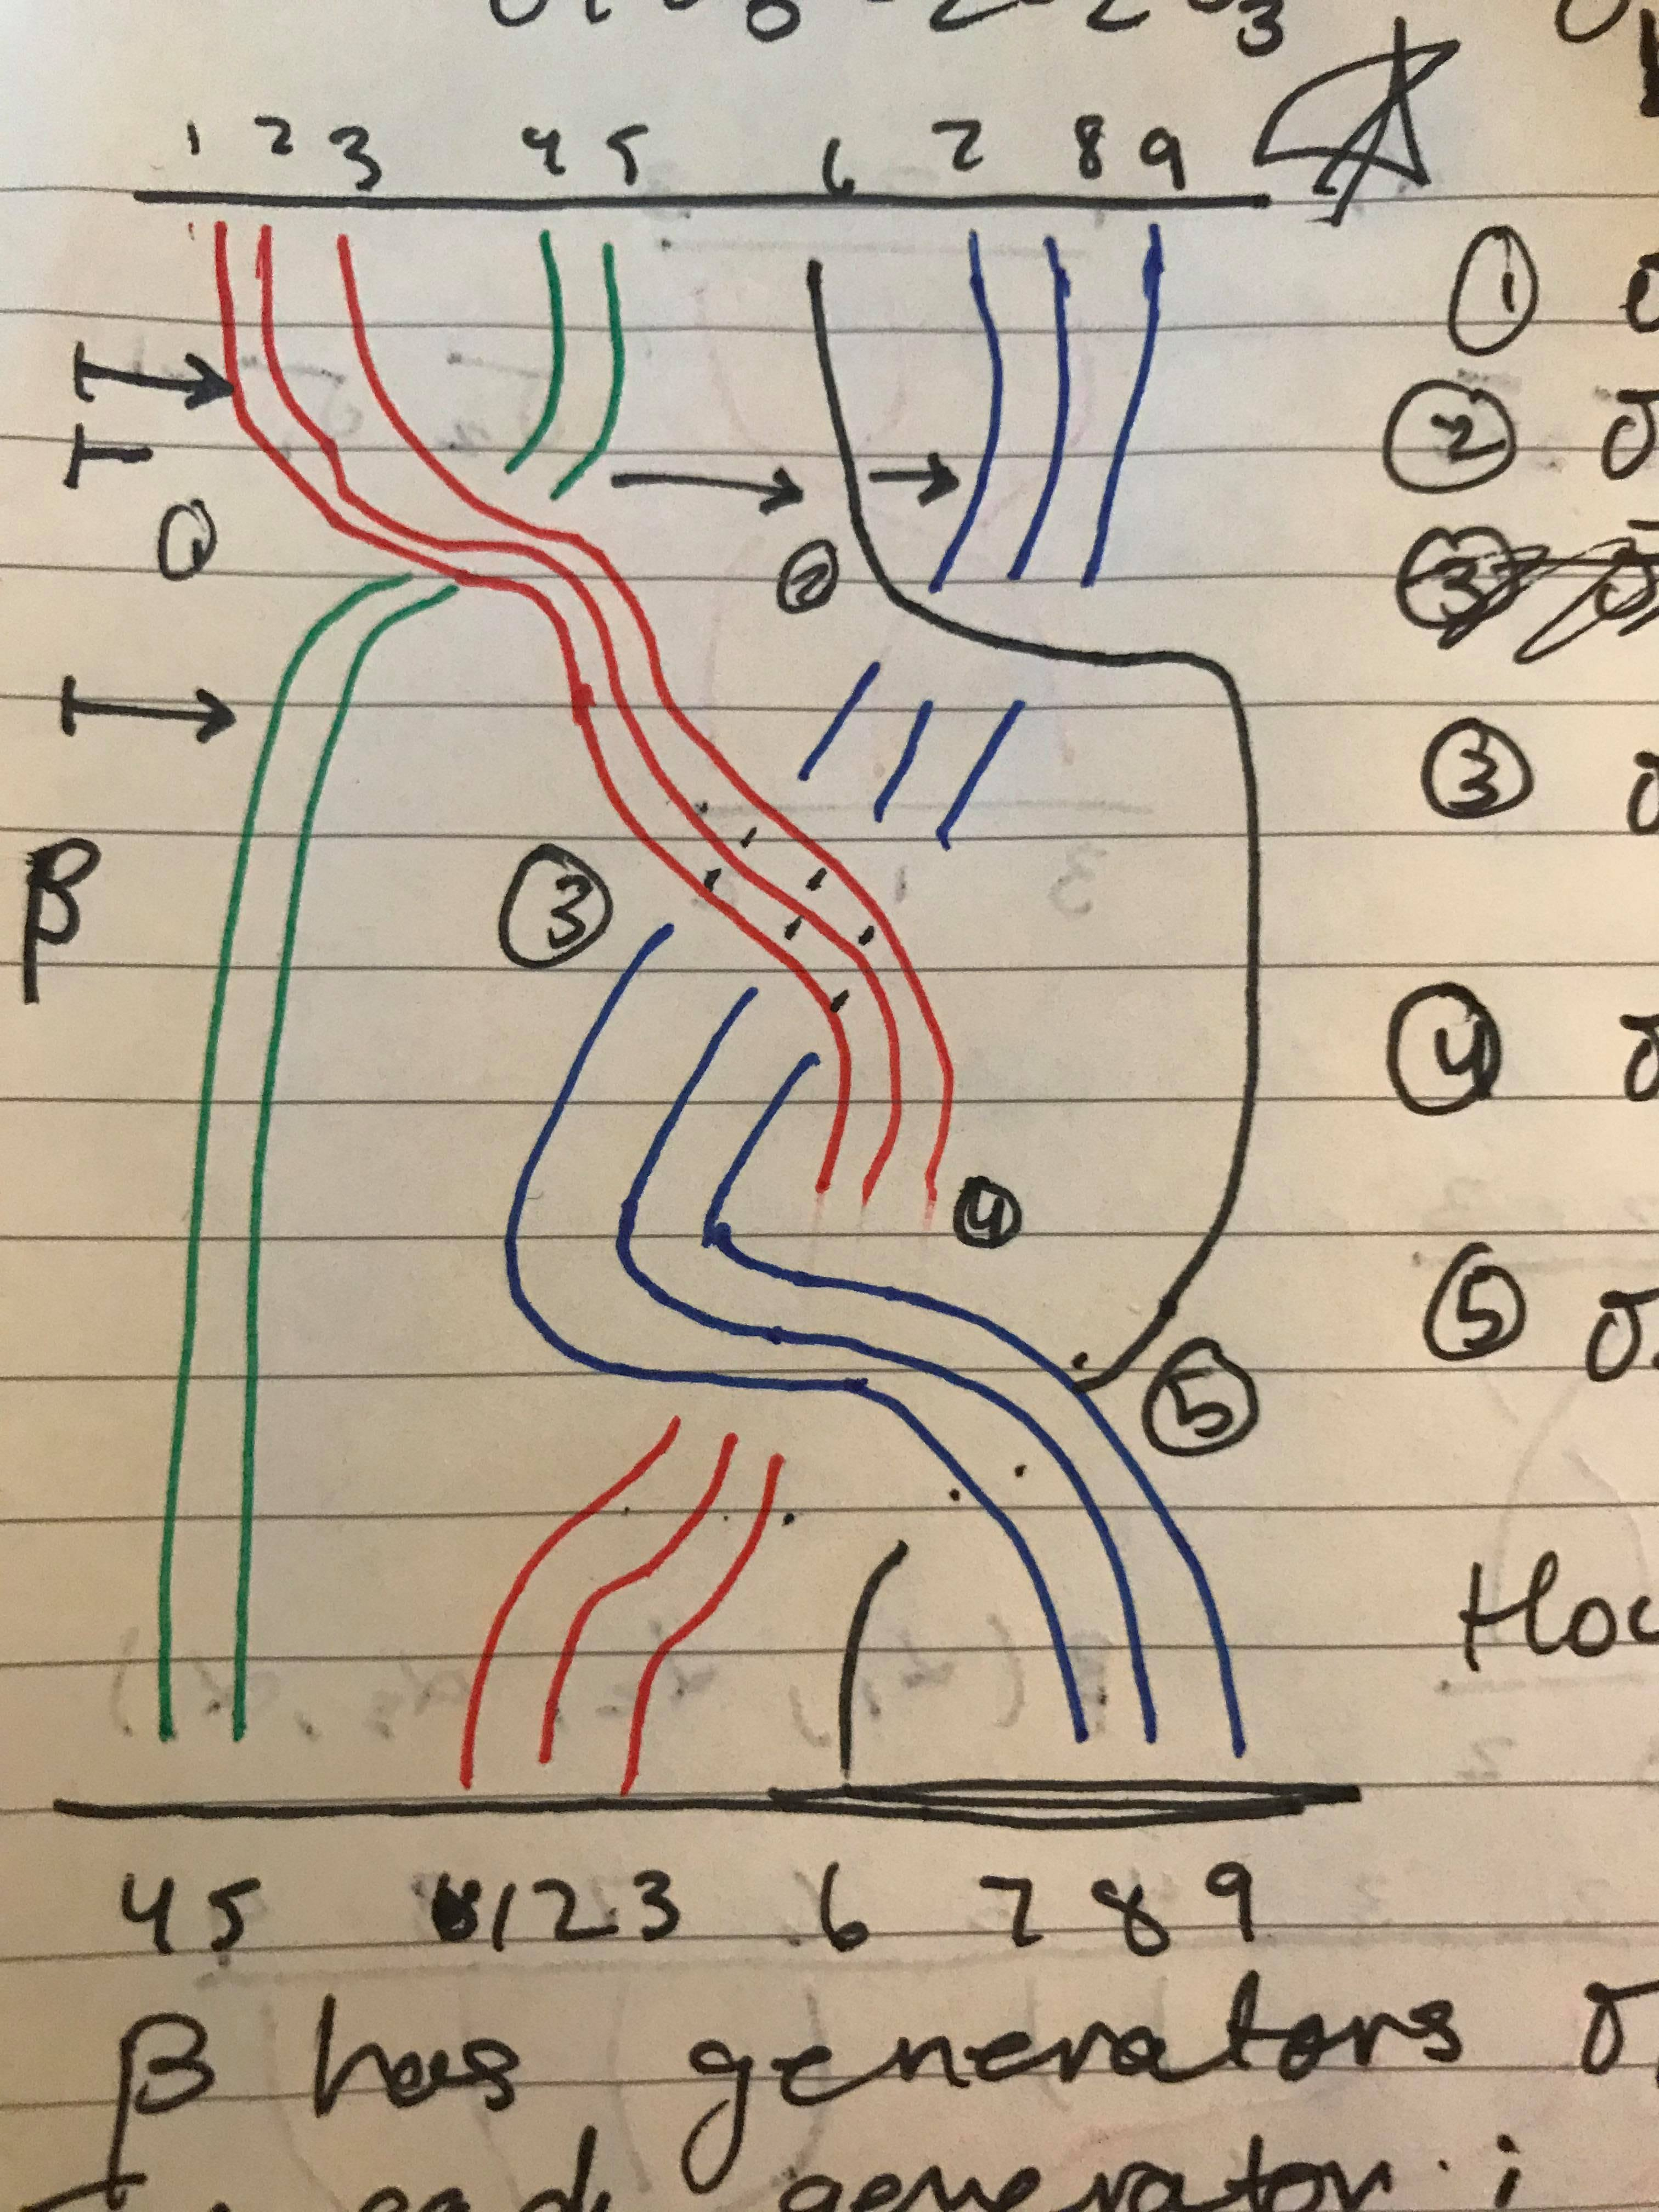
\includegraphics[scale = 0.05]{chp9_operads/braids.jpg}
    
    \emph{Above is the output of $\beta(3, 2, 1, 3)$.}
\end{center}
Staring at the diagram, we can see that it may be expressed as
\begin{gather*}
    (\sigma_3\sigma_2\sigma_1 \cdot \sigma_4\sigma_3\sigma_2) (\sigma_6\sigma_7\sigma_8) 
    (\sigma_5\sigma_4\sigma_3 \cdot \sigma_6\sigma_5\sigma_4 \cdot \sigma_7\sigma_6\sigma_5)\\
    (\sigma_5\sigma_4\sigma_3 \cdot \sigma_6\sigma_5\sigma_4 \cdot \sigma_7\sigma_6\sigma_5)
    (\sigma_8 \sigma_7 \sigma_6).
\end{gather*}
But how can we do this in general? To explain, first suppose 
\[
    \beta = \sigma_{i_1}\sigma_{i_2}\cdots\sigma_{i_k}.
\]
To draw the cabled braid $\beta(k_1, k_2, \dots, k_n)$, we see that we have $k$-crossings to focus on; 
these are where the crossings will happen in our cabled braid. For example, in the braid we provided above, we 
can highlight the crossings in yellow.
\begin{center}
    \def\bottomYCoord{5.5}
\begin{tikzpicture}
    \braid[number of strands= 2, thick,
    style strands={1}{red},
    style strands={2}{Green},
    style strands={3}{Purple},
    style strands={4}{RoyalBlue}]
    (braid) s_1 s_3 s_2 s_2 s_3;
    \filldraw[yellow, opacity = 0.6] (1.5,-0.7) circle (0.3cm);
    \draw (1.5,-0.7) circle (0.3cm);
    \filldraw[yellow, opacity = 0.6] (3.5,-1.7) circle (0.3cm);
    \draw (3.5,-1.7) circle (0.3cm);
    \filldraw[yellow, opacity = 0.6] (2.5,-2.7) circle (0.3cm);
    \draw (2.5,-2.7) circle (0.3cm);
    \filldraw[yellow, opacity = 0.6] (2.5,-3.7) circle (0.3cm);
    \draw (2.5,-3.7) circle (0.3cm);
    \filldraw[yellow, opacity = 0.6] (3.5,-4.7) circle (0.3cm);
    \draw (3.5,-4.7) circle (0.3cm);
    \draw[thick] (0.8,0) -- (4.2,0);
    \draw[thick] (0.8,-\bottomYCoord) -- (4.2,-\bottomYCoord);
\end{tikzpicture}
\end{center}
At each crossing, we're going to have something like this: 
\begin{center}
    \def\bottomYCoord{8.5}
    \begin{tikzpicture}
        \draw[thick] (0.8,0) -- (8.2,0);
        \draw[thick] (0.8,-\bottomYCoord) -- (8.2,-\bottomYCoord);
        \node at (5, -4.2) {
            \begin{tikzpicture}
                \draw[RoyalBlue, thick] plot[smooth,domain=-1.45:1] (\x, {2*\x*\x*\x});
            \end{tikzpicture}
        };
        \node at (5.2, -4.3) {
            \begin{tikzpicture}
                \draw[RoyalBlue, thick] plot[smooth,domain=-1.45:1] (\x, {2*\x*\x*\x});
            \end{tikzpicture}
        };
        \node at (5.5, -4.4) {
            \begin{tikzpicture}
                \draw[RoyalBlue, thick] plot[smooth,domain=-1.35:1.1] (\x, {2*\x*\x*\x});
            \end{tikzpicture}
        };
        %%%%% gaps for braid
        \node at (4.7, -3.9) {
            \begin{tikzpicture}
                \draw[line width = 2mm, white] plot[smooth,domain=-1:1.4] (\x, {-2*\x*\x*\x});
            \end{tikzpicture}
        };
        \node at (4.5, -4) {
            \begin{tikzpicture}
                \draw[line width = 2mm, white] plot[smooth,domain=-1.05:1.4] (\x, {-2*\x*\x*\x});
            \end{tikzpicture}
        };
        \node at (4.1, -4.6) {
            \begin{tikzpicture}
                \draw[line width = 2mm, white] plot[smooth,domain=-1.12:1.32] (\x, {-2*\x*\x*\x});
            \end{tikzpicture}
        };

        %%%%%%% second set of braids
        \node at (4.7, -3.9) {
            \begin{tikzpicture}
                \draw[Red, thick] plot[smooth,domain=-1:1.4] (\x, {-2*\x*\x*\x});
            \end{tikzpicture}
        };
        \node at (4.5, -4) {
            \begin{tikzpicture}
                \draw[Red, thick] plot[smooth,domain=-1.05:1.4] (\x, {-2*\x*\x*\x});
            \end{tikzpicture}
        };
        \node at (4.1, -4.6) {
            \begin{tikzpicture}
                \draw[Red, thick] plot[smooth,domain=-1.12:1.32] (\x, {-2*\x*\x*\x});
            \end{tikzpicture}
        };
        \node at (5,-0.5){
            \begin{tikzpicture}
                \filldraw[white] (0,0) rectangle (9,0.8);
            \end{tikzpicture}
        };
        \node at (5,-8){
            \begin{tikzpicture}
                \filldraw[white] (0,0) rectangle (9,0.8);
            \end{tikzpicture}
        };
        \node at (4, -2.7) {$\vdots$};
        \node at (5.7, -2.7) {$\vdots$};
        \node at (5, -1.7) {$\sigma_{??}$};
    \end{tikzpicture}
\end{center}

That is, at each crossing, there will be a number of red strands crossing over 
blue strands. If we can just describe each of these 
crossings using generators $\sigma_j$ like we did before, 
then we can describe the whole braid. 

We now face the main problem. To describe an arbitrary crossing, we need to know 
which generators $\sigma_1, \sigma_2, \dots, \sigma_{k_1 + \cdots + k_n}$ 
to use, and in general it's not clear which ones to use. For example, 
how do we describe the first crossing? We don't know, so we'll write $\sigma_{??}$. 
If, however, we know that the first red strand is, say the $k$-th strand in $\beta(k_1, \dots, k_n)$,
then we can write the crossing as $\sigma_k$. Then we can travel down the blue line, 
writing $\sigma_{k-1}, \sigma_{k - 2}, \dots$ until we've hit all the red strands. Then 
we can repeat this process for each blue line.

So to do this in general, we need to answer three questions:
\begin{itemize}
    \item How far are all of our red strands from the left? 
    \item How many red strands are there?
    \item How many blue strands are there?
\end{itemize}
If we can answer those three questions, then we can describe exactly what happens 
in terms of generators using formula (\ref{sigma_1_cabling}).

We answer the first question:
\begin{definition}
    Let $\beta \in B_n$ be a braid. Suppose $\beta$ can be written 
    as a product of $k$-many generators $\beta = \sigma_{i_1}\sigma_{i_2} \cdots \sigma_{i_k}$  
    (where any $\sigma$ is equally possibly an inverse). 
    Then we define the quantity 
    \[
        \phi(\sigma_{i_1}\sigma_{i_2}\dots, \sigma_{i_j}, s)
        = 
        \begin{cases}
            \text{The order which strand }s\\
            \text{is from the left after generators}\\
            \sigma_{i_1}\sigma_{i_2}\dots, \sigma_{i_j}
            \text{ have been applied.}
        \end{cases}
    \]
    Of course, $\phi(-, s) = s$, where $-$ represent empty input,
    for each strand $s$. This is because each $s$-th strand is originally the 
    $s$-th strand.

    However, a way to define this is to calculate the underlying permutation 
    of $\sigma_i^{1}\sigma_j^{2}\dots, \sigma_k^{p}$ using the natural projection 
    map $\pi: B_n \to S_n$. Hence we see that 
    \[
        \phi(\sigma_{i_1}\sigma_{i_2}\dots, \sigma_{i_k}, s)
        = 
        \pi(\sigma_{i_1}\sigma_{i_2}\dots, \sigma_{i_k})(s).
    \]
\end{definition}

\begin{example}
    Consider the braid $\sigma_1\sigma_3\sigma_2\sigma_2\sigma_3$ pictured below.
    Suppose we've applied $\sigma_1\sigma_3$. Then our braids are now reordered from how 
    they were initially positioned. For instance, after the application of these 
    generators, the green strand is now the first strand; the red strand is now 
    the second; the blue strand is the third; and the black strand is now the fourth. 
    Each color strand is now in a different position than which it started in.
    \begin{center}
        \def\bottomYCoord{5.5}
        \begin{tikzpicture}
            \braid[number of strands= 2, thick,
            style strands={1}{red},
            style strands={2}{Green},
            style strands={3}{Purple},
            style strands={4}{RoyalBlue}]
            (braid) s_1 s_3 s_2 s_2 s_3;
            \filldraw[yellow, opacity = 0.6] (1.5,-0.7) circle (0.3cm);
            \draw (1.5,-0.7) circle (0.3cm);
            \filldraw[yellow, opacity = 0.6] (3.5,-1.7) circle (0.3cm);
            \draw (3.5,-1.7) circle (0.3cm);
            \draw[thick] (0.8,0) -- (4.2,0);
            \draw[thick] (0.8,-\bottomYCoord) -- (4.2,-\bottomYCoord);
        \end{tikzpicture}
    \end{center}
    However, we can express this observation using our tool.
    Note that $\pi(\sigma_1\sigma_3)$ is the permutation $(1, 2, 3, 4) \mapsto 
    (2, 1, 4, 3)$. Hence we see that 
    \[
        \phi(\sigma_1\sigma_3, 1) = \textcolor{Green}{2} \quad \phi(\sigma_1\sigma_3, 2) = \textcolor{Red}{1} \quad
        \phi(\sigma_1\sigma_3, 3) = \textcolor{RoyalBlue}{4} \quad \phi(\sigma_1\sigma_3, 4) = \textcolor{Purple}{3}.
    \] 
    What about after the first three generators have been applied? We calculate 
    again: $\pi(\sigma_1\sigma_3\sigma_2)$ is the permutation $(1, 2, 3, 4) \mapsto (2, 4, 1, 3)$.
    Hence we have that 
    \[
        \phi(\sigma_1\sigma_3\sigma_2, 1) = \textcolor{Green}{2} \quad \phi(\sigma_1\sigma_3\sigma_2, 2) = \textcolor{NavyBlue}{4} \quad
        \phi(\sigma_1\sigma_3\sigma_2, 3) = \textcolor{red}{1} \quad \phi(\sigma_1\sigma_3\sigma_2, 4) = \textcolor{Purple}{3}.
    \]
    which matches a simple hand-count that we can perform using the picture below.
    \begin{center}
        \begin{tikzpicture}
            \def\bottomYCoord{5.5}
            \braid[number of strands= 2, thick,
            style strands={1}{red},
            style strands={2}{Green},
            style strands={3}{Purple},
            style strands={4}{RoyalBlue}]
            (braid) s_1 s_3 s_2 s_2 s_3;
            \filldraw[yellow, opacity = 0.6] (1.5,-0.7) circle (0.3cm);
            \draw (1.5,-0.7) circle (0.3cm);
            \filldraw[yellow, opacity = 0.6] (3.5,-1.7) circle (0.3cm);
            \draw (3.5,-1.7) circle (0.3cm);
            \filldraw[yellow, opacity = 0.6] (2.5,-2.7) circle (0.3cm);
            \draw (2.5,-2.7) circle (0.3cm);
            \draw[thick] (0.8,0) -- (4.2,0);
            \draw[thick] (0.8,-\bottomYCoord) -- (4.2,-\bottomYCoord);
        \end{tikzpicture}
    \end{center}
\end{example}

This tool allows us to answer our second and third questions. For example, consider again 
$\beta(3, 2, 1, 3)$ where $\beta = \sigma_1\sigma_3\sigma_2\sigma_2\sigma_3$. 
How do we calculate, 
for example, the crossing \raisebox{-0.1cm}{$\begin{tikzpicture}\draw (0,0.2) circle(0.2cm) node {5};\end{tikzpicture}$},
of 3 blue lines over 1 black line, as in the picture below?

\begin{center}
    \begin{tikzpicture}
        \braid[number of strands= 2, thick,
        style strands={1}{red},
        style strands={2}{Green},
        style strands={3}{Black},
        style strands={4}{RoyalBlue}]
        (braid) s_1 s_3 s_2 s_2 s_3;
    \end{tikzpicture}
    \hspace{1cm}
    \raisebox{2cm}{$\mapsto$}
    \hspace{1cm}
    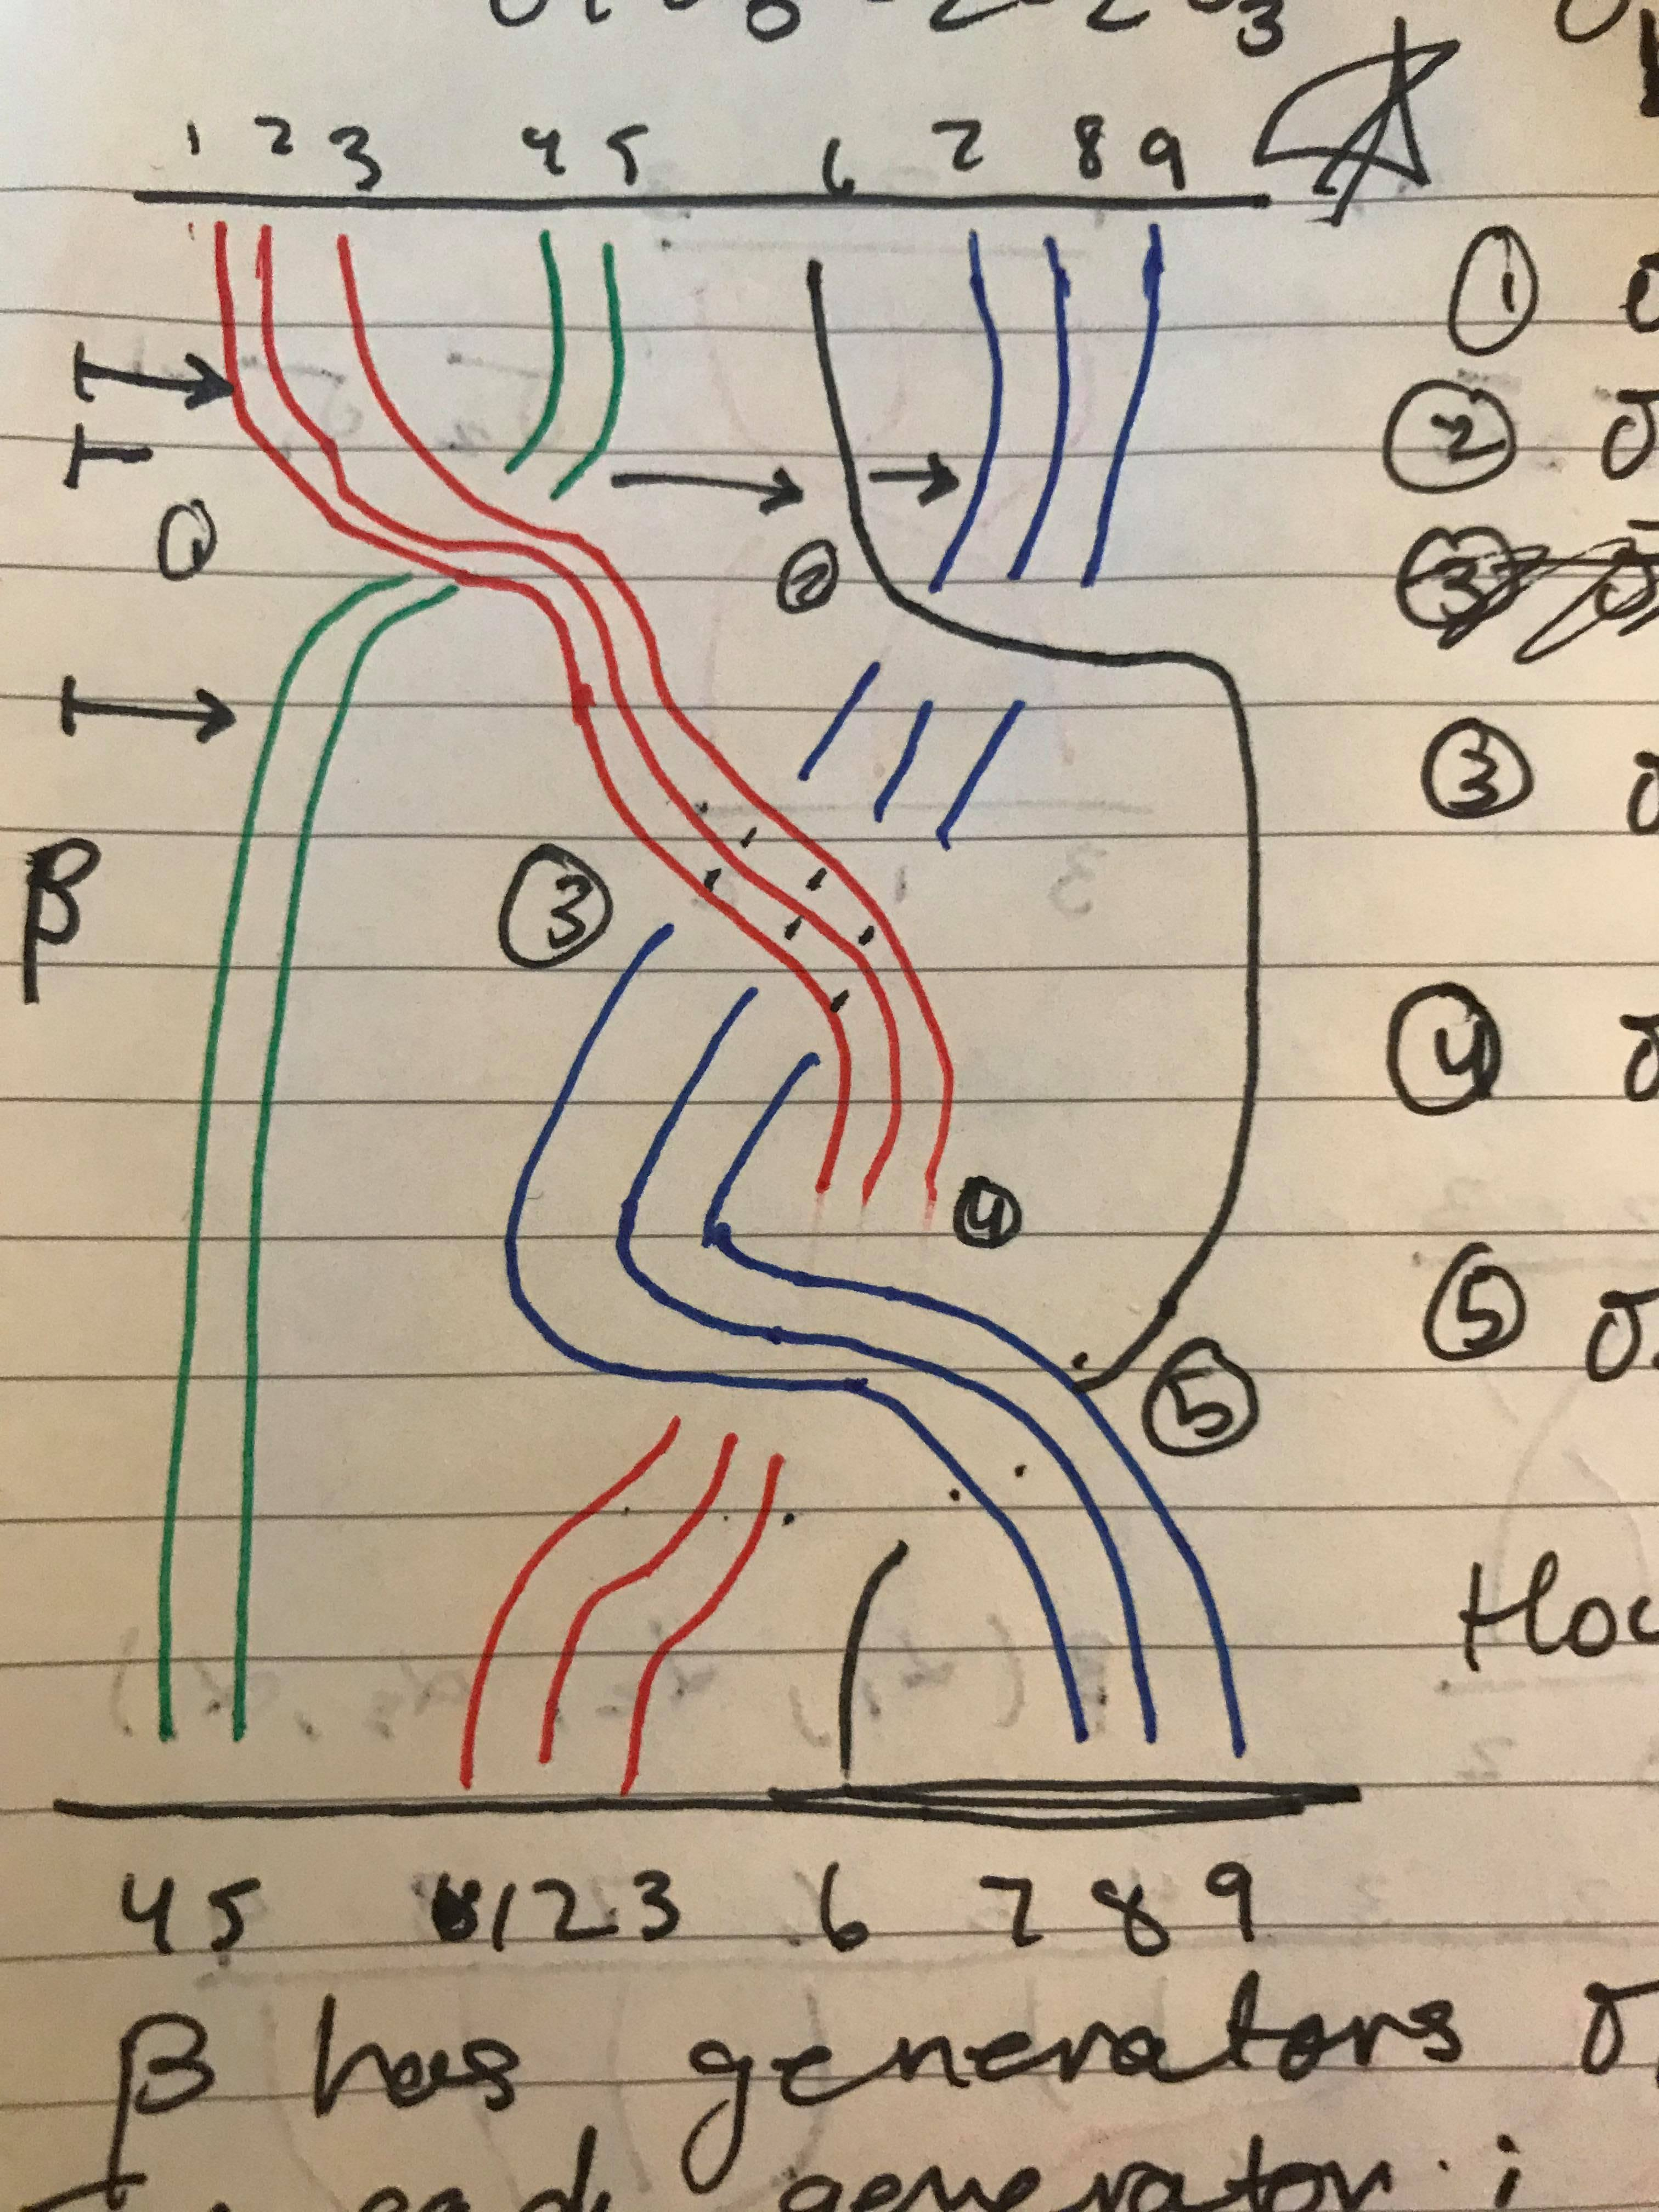
\includegraphics[scale = 0.05]{chp9_operads/braids.jpg}
    
    \emph{Above is the output of $\beta(3, 2, 1, 3)$.}
\end{center}
This crossing is induced by $\sigma_3$, the fifth generator of $\beta$. 
Hence $\beta$ tells us to cross the $3$nd cable over the $4$rd cable. But what 
are these cables? From looking at the diagram, we definitely know. But in general we won't 
be able to just look at the diagram. However, our tool can tell us: Since we've applied $\sigma_1\sigma_3\sigma_2\sigma_2$, 
we see that 
\[
    \phi(\sigma_1\sigma_3\sigma_2\sigma_2, 3) = \textcolor{RoyalBlue}{4} \qquad \phi(\sigma_1\sigma_3\sigma_2\sigma_2, 4) = \textcolor{Black}{1}.
\]
Therefore, we're crossing blue cables over the black cables. We also now know there
are $k_{\textcolor{RoyalBlue}{4}} = 3$ blue cables and $k_{\textcolor{Black}{3}} = 1$ many black cables.
We have almost everything we need except the following: how far 
are the blue cables from the left of the diagram? 

Well, since the blue strands are inside of the third cable, we just need to ask how many 
stands are in the first and second cables. But what is the first cable? What's the second?
We see that
\[
    \phi(\sigma_1\sigma_3\sigma_2\sigma_2, 1) =  \textcolor{Green}{2}.
    \quad 
    \phi(\sigma_1\sigma_3\sigma_2\sigma_2, 2) = \textcolor{Red}{1}.
\]
Hence there are 
\[
    k_{\textcolor{Green}{2}} + k_{\textcolor{Red}{1}} = 2 + 3 = 5    
\]
strands before the blue strands. We can now calculate the crossings: 
\begin{align*}
    \sigma_{5 + 3}\sigma_{5 + 2} \sigma_{5 + 1}
    &=
    \prod_{m = 1 + 5}^{1 + 5}\sigma_{3 + (m - 1)}\sigma_{3 + (m - 2)}\sigma_m\\
    &=
    \prod_{m = p}^{p + (r - 1)}\sigma_{q + (m - 1)}\sigma_{q + (m - 2)}\sigma_m
\end{align*}
where 
\[
    p = 1 + \hspace{-1.5cm}\overbrace{k_2 + k_3}^{\text{\# of strands before the red strands}}
    \quad 
    q = \hspace{-1cm}\underbrace{k_{\textcolor{RoyalBlue}{4}}}_{\text{\# of strands in the 3rd cable}}
    r = \hspace{-1cm}\overbrace{k_{\textcolor{Black}{3}}}^{\text{\# of strands in the 4th cable}}
\]


Therefore we propose the following. 
\begin{lemma}
    Let $\beta \in B_n$ be a braid, and suppose it 
    may be expressed as $\sigma_{i_1}\sigma_{i_2} \cdots \sigma_{i_k}$ in terms of $k$-many 
    generators. Let $k_1, \dots, k_n$ be positive integers. Then we have that 
    \[
        \beta(k_1, k_2, \dots, k_n) 
        = 
        \psi_1\psi_2\dots\psi_k
    \]  
    where, depending on if $\sigma_{i_j}$ is an instance of an inverse or not, 
    we have 
    \begin{statement}{ProcessBlue!10}
    \[
        \prod_{m = p_j}^{p_j + (r_j-1)}
        \sigma_{q_j + (m-1)}
        \sigma_{q_j + (m-2)}
        \cdots 
        \sigma_{m}
        \quad 
        \text{ or }
        \quad 
        \prod_{m = p_j}^{p_j + (r_j-1)}
        \sigma^{-1}_{(q_j + m) - 1}
        \sigma^{-1}_{(q_j -m) - 2}
        \cdots 
        \sigma^{-1}_{m}
    \]
    \end{statement}
    where in both cases
    \begin{statement}{ProcessBlue!10}
    \[
        p_j
        =
        \overbrace{
        1 +
        \sum_{u = 1}^{i_j-1}
        k_{\phi(\sigma_{i_1}\cdots\sigma_{i_{j-1}}, u)}
        }^{\text{\# strands before } i_j\text{-th cable} }
        \qquad
        \underbrace{
        q_j = 
        k_{\phi(\sigma_{i_1}\cdots\sigma_{i_{j-1}}, i_j)}
        }_{\text{\# of strands in the }i_j \text{-th cable}}
        \qquad 
        \overbrace{
        r_j
        =
        k_{\phi(\sigma_{i_1}\cdots\sigma_{i_{(j-1)}}, (i_j+1))}
        }^{\text{\# of stands in the } (i_j+1)\text{-th cable} }
    \]
    \end{statement}
\end{lemma}

The three quantities are the three answers to our original questions: 
\begin{itemize}
    \item After applying $\sigma_{i_1}\dots\sigma_{i_{j-1}}$,
    how many strands come before the cable $i_j$, relative to the left? $p_j$.
    \item 
    How many strands are in the $i_j$-th cable after applying $\sigma_{i_1}\dots\sigma_{i_{j-1}}$? 
    $q_j$.
    \item How many strands are in the $(i_j+1)$-th after applying $\sigma_{i_1}\dots\sigma_{i_{j-1}}$? 
    $r_j$.
\end{itemize}

\begin{example}
    We can apply this to our previous example. 
    Recall that $\beta = \sigma_1\sigma_3\sigma_2\sigma_2\sigma_3$. 
    One way to interpret out braid diagram is as a sequence of permutations.
    In this case we see that we get five permutations because we have five generators.
    \begin{center}
        \def\bottomYCoord{5.5}
        \begin{tikzpicture}
            \braid[number of strands= 2, thick,
            style strands={1}{red},
            style strands={2}{Green},
            style strands={3}{Purple},
            style strands={4}{RoyalBlue}]
            (braid) s_1 s_3 s_2 s_2 s_3;
            % \filldraw[yellow, opacity = 0.6] (1.5,-0.7) circle (0.3cm);
            % \draw (1.5,-0.7) circle (0.3cm);
            % \filldraw[yellow, opacity = 0.6] (3.5,-1.7) circle (0.3cm);
            % \draw (3.5,-1.7) circle (0.3cm);
            \draw[thick] (0.8,0) -- (4.2,0);
            \draw[thick] (0.8,-\bottomYCoord) -- (4.2,-\bottomYCoord);
            \node at (1, -5.7) {\phantom{2}};
            \node at (2, -5.7) {\phantom{1}};
            \node at (3, -5.7) {\phantom{4}};
            \node at (4, -5.7) {\phantom{3}};
        \end{tikzpicture}
        \raisebox{3cm}{$\mapsto$}
        \begin{tikzpicture}
            \braid[number of strands= 2, thick,
            style strands={1}{red},
            style strands={2}{Green},
            style strands={3}{Purple},
            style strands={4}{RoyalBlue}]
            (braid) s_1 s_3 s_2 s_2 s_3;
            % \filldraw[yellow, opacity = 0.6] (1.5,-0.7) circle (0.3cm);
            % \draw (1.5,-0.7) circle (0.3cm);
            % \filldraw[yellow, opacity = 0.6] (3.5,-1.7) circle (0.3cm);
            % \draw (3.5,-1.7) circle (0.3cm);
            \draw[thick] (0.8,0) -- (4.2,0);
            \draw (0.8,-1.4) -- (4.2,-1.4); %first bar
            \draw (0.8,-2.3) -- (4.2,-2.3); %second bar
            \draw (0.8,-3.3) -- (4.2,-3.3); %third bar
            \draw (0.8,-4.3) -- (4.2,-4.3); %fourth bar
            
            %first set
            \node at (1, 0.2) {1};
            \node at (2, 0.2) {2};
            \node at (3, 0.2) {3};
            \node at (4, 0.2) {4};
            %second set
            \node at (1.2, -1.2) {2};
            \node at (2.2, -1.2) {1};
            \node at (3.2, -1.2) {3};
            \node at (4.2, -1.2) {4};
            %third set 
            \node at (1.2, -2.1) {2};
            \node at (2.2, -2.1) {1};
            \node at (3.2, -2.1) {4};
            \node at (4.2, -2.1) {3};
            %fourth set 
            \node at (1.2, -3.1) {2};
            \node at (2.2, -3.1) {4};
            \node at (3.2, -3.1) {1};
            \node at (4.2, -3.1) {3};
            %fifth set 
            \node at (1.2, -4.1) {2};
            \node at (2.2, -4.1) {1};
            \node at (3.2, -4.1) {4};
            \node at (4.2, -4.1) {3};
            %sixth set 
            \node at (1, -5.7) {2};
            \node at (2, -5.7) {1};
            \node at (3, -5.7) {3};
            \node at (4, -5.7) {4};
            \draw[thick] (0.8,-\bottomYCoord) -- (4.2,-\bottomYCoord);
        \end{tikzpicture}
    \end{center}

    First we compute the table 
    \begin{center}
        \begin{tabular}{|c|c |c| c| c|} 
            \hline
            $j$ & $i_{j}$ & $p_j$ & $q_j$ & $r_j$ \\ [0.5ex] 
            \hline
            1 & 1 & 1 &$k_1 = 3$ & $k_2 = 2$ \\ 
            \hline
            2 & 3 & $1 + k_1 + k_2 = 6$ & $k_3 = 1$ & $k_4 = 3$ \\
            \hline
            3 & 2 & $1 + k_2 = 3$ & $k_1 = 3$ & $k_4 = 3$ \\
            \hline
            4 & 2 & $1 + k_2 = 3$ & $k_4 = 3$ & $k_1 = 3$ \\
            \hline
            5 & 3 & $1 + k_1 + k_2 = 6$ & $k_4 = 3$ & $k_3 = 1$ \\ [1ex] 
            \hline
           \end{tabular}
    \end{center}
    This then gives us the product 
    \begin{gather*}
        \left(\prod_{m = p_1}^{p_1 + (r_1-1)}
        \sigma_{q_1 + (m-1)}
        \sigma_{q_1 + (m-2)}
        \cdots 
        \sigma_{m}\right)
        \left(\prod_{m = p_2}^{p_2 + (r_2-1)}
        \sigma_{q_2 + (m-1)}
        \sigma_{q_2 + (m-2)}
        \cdots 
        \sigma_{m} \right)
        \\
        \left(     \prod_{m = p_3}^{p_3 + (r_3-1)}
        \sigma_{q_3 + (m-1)}
        \sigma_{q_3 + (m-2)}
        \cdots 
        \sigma_{m} \right)
        \\
        \left(    \prod_{m = p_4}^{p_4 + (r_4-1)}
        \sigma_{q_4 + (m-1)}
        \sigma_{q_4 + (m-2)}
        \cdots 
        \sigma_{m} \right)
        \left(     \prod_{m = p_5}^{p_5 + (r_5-1)}
        \sigma_{q_5 + (m-1)}
        \sigma_{q_5 + (m-2)}
        \cdots 
        \sigma_{m} \right)
    \end{gather*}
    which becomes 
    \begin{gather*}
        \left(\prod_{m = 1}^{1 + (2-1)}
        \sigma_{3 + (m-1)}
        \sigma_{3 + (m-2)}
        \cdots 
        \sigma_{m}\right)
        \left(\prod_{m = 6}^{6 + (3-1)}
        \sigma_{1 + (m-1)}
        \sigma_{1 + (m-2)}
        \cdots 
        \sigma_{m} \right)
        \\
        \left(     \prod_{m = 3}^{3 + (3-1)}
        \sigma_{3 + (m-1)}
        \sigma_{3 + (m-2)}
        \cdots 
        \sigma_{m} \right)
        \\
        \left(    \prod_{m = 3}^{3 + (3-1)}
        \sigma_{3 + (m-1)}
        \sigma_{3 + (m-2)}
        \cdots 
        \sigma_{m} \right)
        \left(     \prod_{m = 6}^{6 + (1-1)}
        \sigma_{3 + (m-1)}
        \sigma_{3 + (m-2)}
        \cdots 
        \sigma_{m} \right)
    \end{gather*}
    which reduces to 
    \begin{gather*}
        (\sigma_3\sigma_2\sigma_1 \cdot \sigma_4\sigma_3\sigma_2)
        (\sigma_6 \sigma_7\sigma_8)(\sigma_5\sigma_4\sigma_3\cdot \sigma_6\sigma_5\sigma_4 \cdot \sigma_7\sigma_6\sigma_5)
        \\
        (\sigma_5\sigma_4\sigma_3\cdot \sigma_6\sigma_5\sigma_4 \cdot \sigma_7\sigma_6\sigma_5)
        (\sigma_8\sigma_7\sigma_6)
    \end{gather*}
    which correctly matches what we had before. 
\end{example}

\begin{example}
    We haven't looked at a braid with an under crossing. So, 
    consider the braid $\beta = \sigma_1^{-1}\sigma_2^{-1}\sigma_3\sigma_2\sigma_1 \in B_4$, 
    and let $k_1 = 2, k_2 = 3, k_3 = 4, k_4 = 5$. We'll want to calculate 
    the braid $\beta(2, 3, 4, 5)$. Below is $\beta$ and $\beta(2,3,4,5)$.
    \begin{center}
    \def\bottomYCoord{5.5}
    \begin{tikzpicture}
        \braid[number of strands= 4, thick, 
        style strands={1}{Red},
        style strands={2}{Green},
        style strands={3}{Purple},
        style strands={4}{RoyalBlue}]
        (braid) s_1^{-1} s_2^{-1} s_3 s_2 s_1;
        \draw[thick] (0.8,0) -- (4.2,0);
        \draw[thick] (0.8,-\bottomYCoord) -- (4.2,-\bottomYCoord);
    \end{tikzpicture}
    \hspace{1cm}
    \raisebox{2cm}{$\mapsto$}
    \hspace{1cm}
    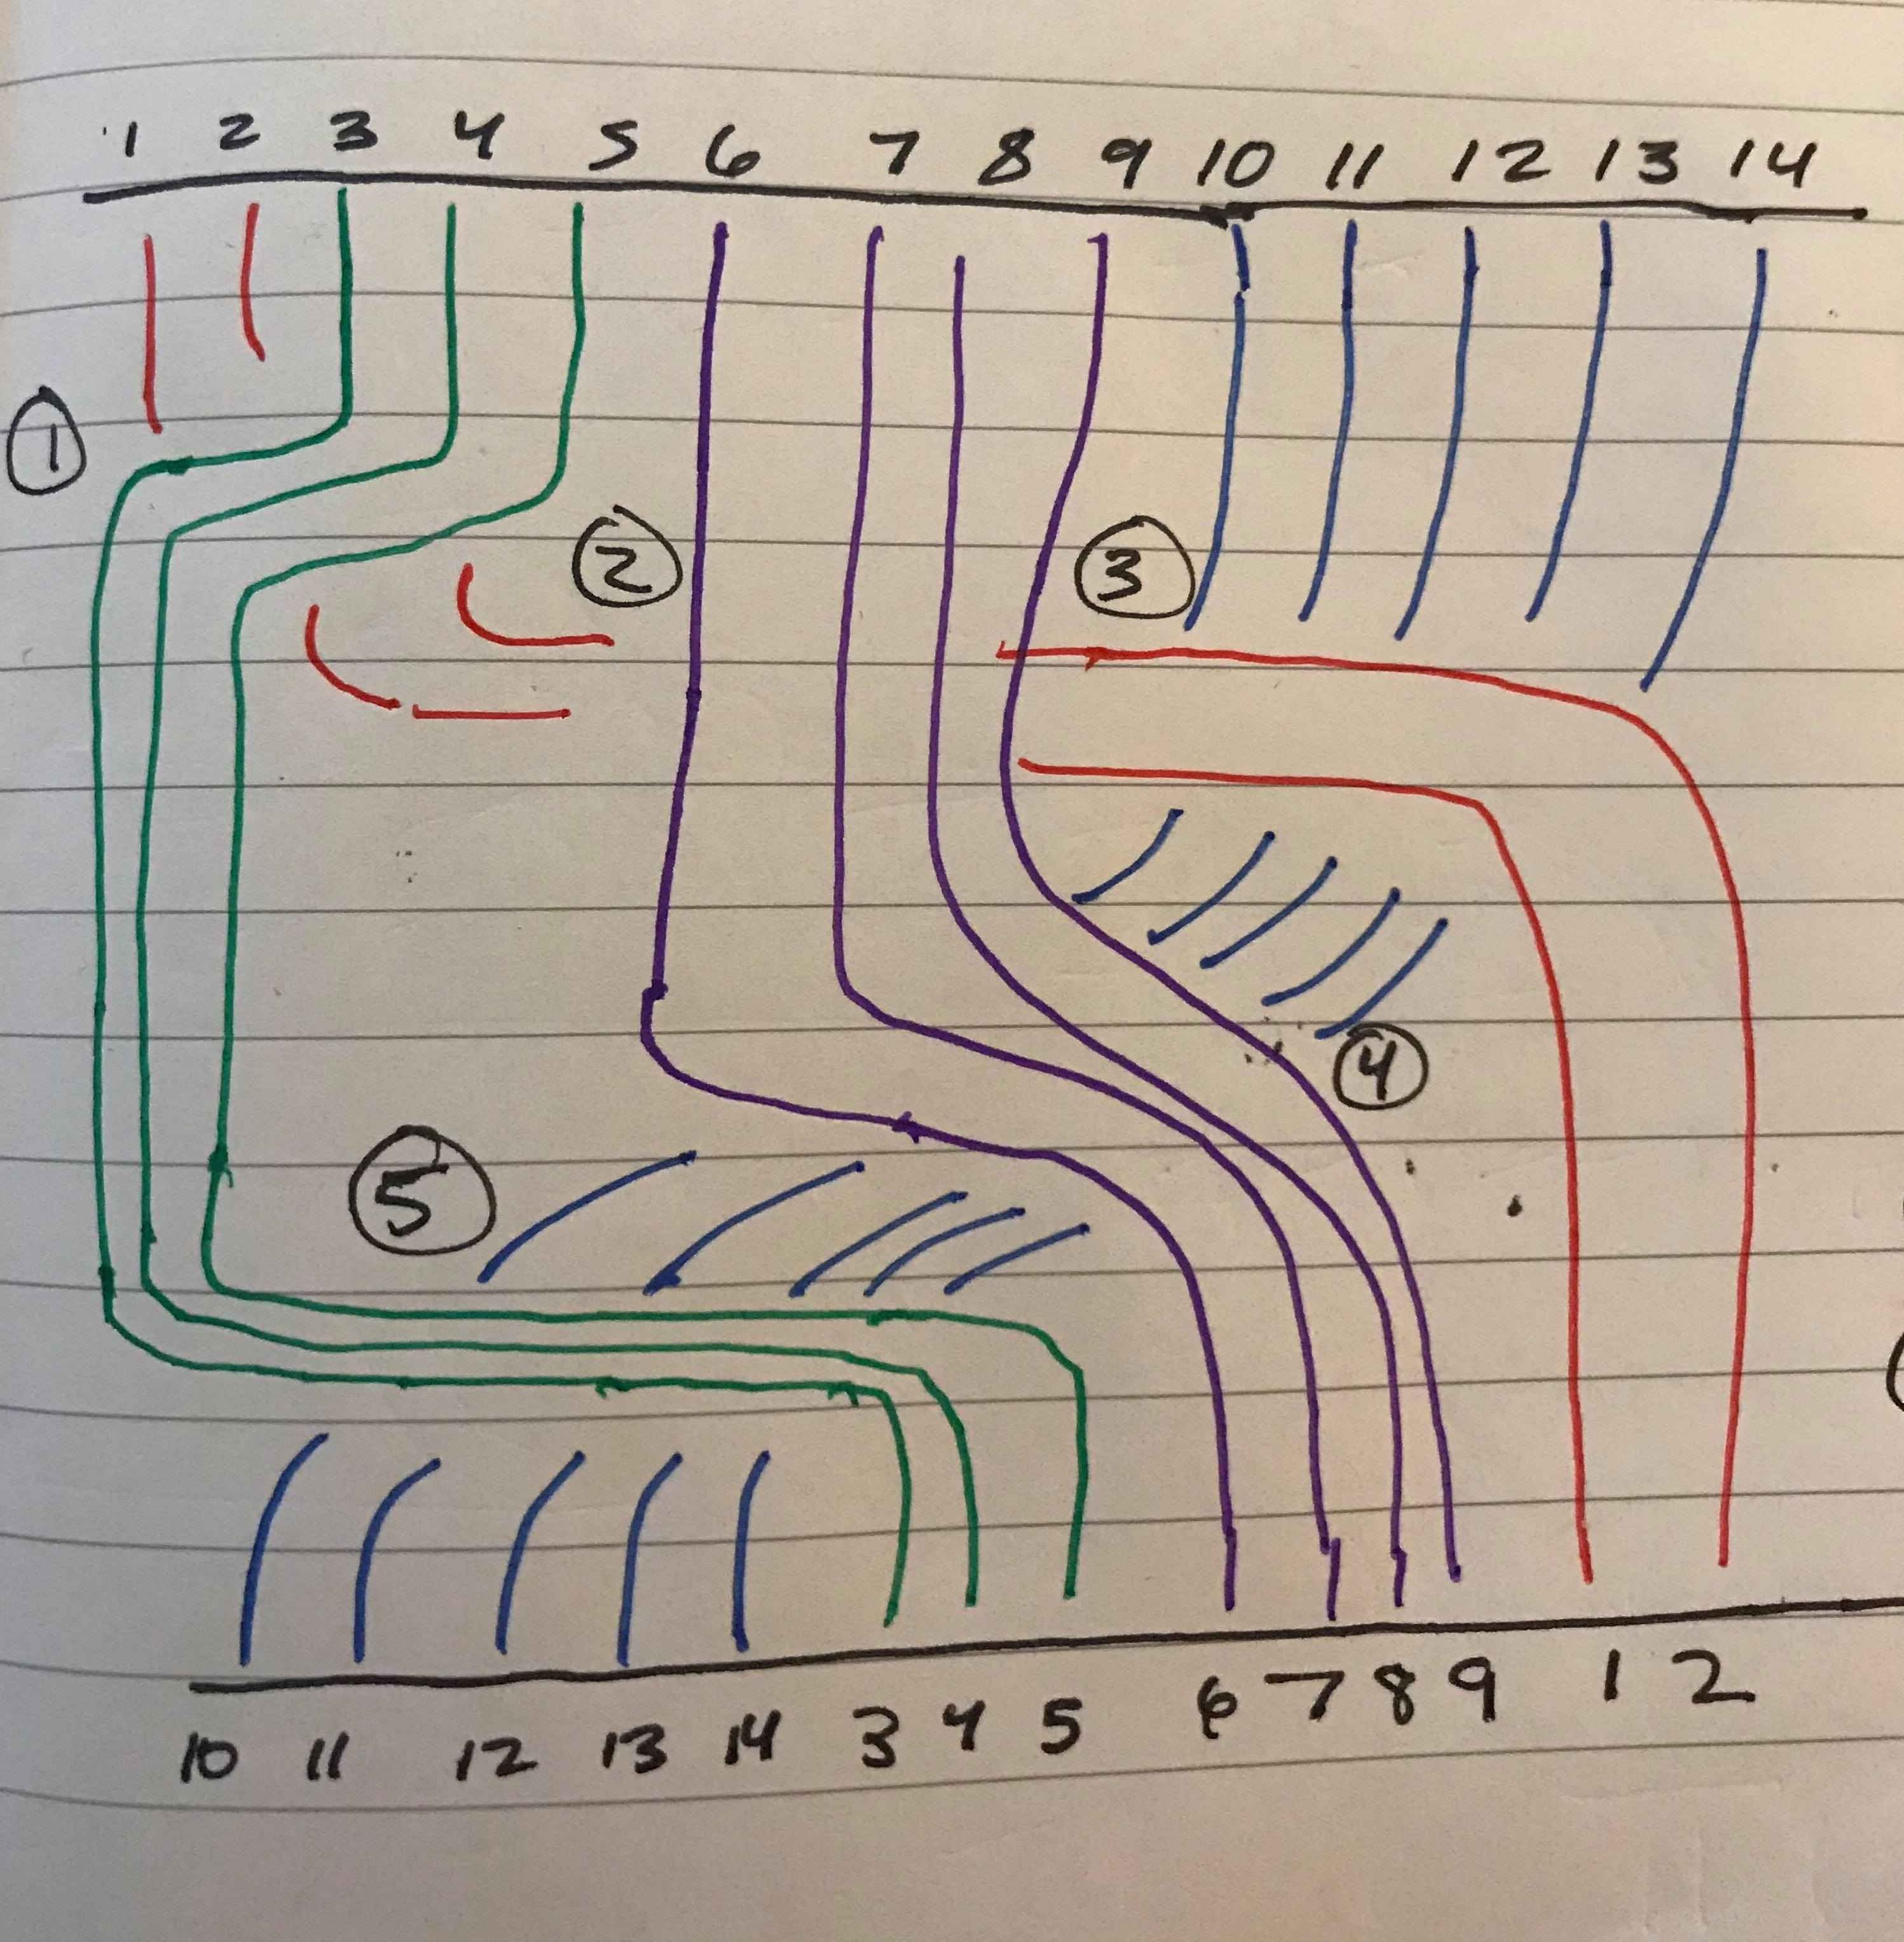
\includegraphics[scale = 0.06]{chp9_operads/inverse_braids.jpg}
    \end{center}
    To calculate the resulting braid we need to create our table of values.
    This is more easily done by generating the permutation table on the left; it 
    tells us how our cables are swapped around. 
    \begin{center}
        \begin{tabular}{|l|c|}
            \hline
            Generator & Permutation\\
            \hline
            $\varnothing$ & $(\textcolor{Red}{1}, \textcolor{Green}{2}, \textcolor{Purple}{3}, \textcolor{RoyalBlue}{4})$\\
            \hline
            $\sigma_1^{-1}$ & $(\textcolor{Green}{2}, \textcolor{Red}{1}, \textcolor{Purple}{3}, \textcolor{RoyalBlue}{4})$\\
            \hline
            $\sigma_1^{-1}\sigma_2^{-1}$ & $(\textcolor{Green}{2}, \textcolor{Purple}{3}, 1, \textcolor{RoyalBlue}{4})$\\
            \hline
            $\sigma_1^{-1}\sigma_2^{-1}\sigma_3$ & $(\textcolor{Green}{2}, \textcolor{Purple}{3}, \textcolor{RoyalBlue}{4}, 1)$\\
            \hline
            $\sigma_1^{-1}\sigma_2^{-1}\sigma_3\sigma_2$ & $(\textcolor{Green}{2}, \textcolor{RoyalBlue}{4}, \textcolor{Purple}{3}, 1)$\\
            \hline
            $\sigma_1^{-1}\sigma_2^{-1}\sigma_3\sigma_2\sigma_1$ & $(\textcolor{RoyalBlue}{4}, \textcolor{Green}{2}, \textcolor{Purple}{3}, 1)$\\
            \hline
        \end{tabular}
        \hspace{1cm}
        \begin{tabular}{|c|c |c| c| c|} 
            \hline
            $j$ & $i_{j}$ & $p_j$ & $q_j$ & $r_j$ \\ [1ex] 
            \hline
            1 & 1 & 1 & $k_1 = 2$  & $k_2 = 3$  \\ [.1ex] 
            \hline
            2 & 2 & $1 + k_2 = 4$ & $k_1 =2$ & $k_3 = 4$ \\ [.1ex] 
            \hline
            3 & 3 & $1 + k_2 + k_3 = 8$ & $k_1 = 2$ & $k_4 = 5$ \\ [.1ex] 
            \hline
            4 & 2 & $1 + k_2 = 4$ & $k_3 =4$ & $k_4 = 5$ \\[.1ex] 
            \hline
            5 & 1 & $1$ & $k_2 = 3$ & $k_4 = 5$\\ [1ex] 
            \hline
           \end{tabular}
    \end{center}
    This then generates the products 
    \begin{gather*}
        \left(\prod_{m = 1}^{3}\sigma_{m + 2}^{-1}\sigma^{-1}_m\right)
        \left( \prod_{m = 4}^{7}\sigma^{-1}_{(m+2)-1}\sigma_m^{-1} \right)
        \left( \prod_{m = 8}^{12}\sigma_{(m+2)-1}\sigma_m \right)
        \left( \prod_{m = 4}^{8}\sigma_{(m+4)-1}\sigma_{(m+4)-2}\sigma_{(m+4)-3}\sigma_{m} \right)
        \\
        \left( \prod_{m = 1}^{5}\sigma_{(m+3)-1}\sigma_{(m+3)-2}\sigma_m \right)
    \end{gather*}
    which becomes 
    \begin{gather*}
        (\sigma^{-1}_2\sigma^{-1}_1 \cdot \sigma^{-1}_3\sigma^{-1}_2 \cdot \sigma^{-1}_4\sigma^{-1}_3)
        (\sigma^{-1}_5\sigma^{-1}_4\cdot \sigma^{-1}_6\sigma^{-1}_5 \cdot \sigma^{-1}_7\sigma^{-1}_6 \cdot \sigma^{-1}_8\sigma^{-1}_7)
        \\
        (\sigma_9\sigma_8 \cdot \sigma_{10}\sigma_9 \cdot \sigma_{11}\sigma_{10} \cdot \sigma_{12}\sigma_{11} \cdot \sigma_{13}\sigma_{12})
        (\sigma_7\sigma_6\sigma_5\sigma_4 \cdot \sigma_8\sigma_7\sigma_6\sigma_5 \cdot \sigma_9\sigma_8\sigma_7\sigma_6 \cdot 
        \sigma_{10}\sigma_9\sigma_8\sigma_7\cdot \sigma_{11}\sigma_{10}\sigma_9\sigma_8)
        \\
        (\sigma_3\sigma_2\sigma_1 \cdot \sigma_4\sigma_3\sigma_2 \cdot \sigma_5\sigma_4\sigma_3 \cdot \sigma_6\sigma_5\sigma_4 \cdot \sigma_7\sigma_6\sigma_5)
    \end{gather*}
    which is the correct description of the braid $\beta(2,3,4,5)$. 
\end{example}

Now we can finally answer our desired question: 
\begin{center}
    Given a braid $\beta \in B_n$, and $n$ other braids $\alpha_1 \in B_{a_1}, \dots, \alpha_n \in B_{a_n}$, 
    what is the formula for $\beta(\alpha_1, \dots, \alpha_n)$? 
\end{center}

To answer this question, we build on our previous work by making the following observation. 
Suppose we want to compute $\sigma_1(\alpha_1, \alpha_2)$ where $\sigma_1, \alpha_1, \alpha_2$
appear as below.
\begin{center}
    \def\bottomYCoord{3.5}
    \begin{tikzpicture}
        \braid[number of strands= 2, thick,  height = 3cm]
        s_1;
        \draw[thick] (0.8,0) -- (2.2,0);
        \draw[thick] (0.8,-\bottomYCoord) -- (2.2,-\bottomYCoord);
    \end{tikzpicture}
    \hspace{1cm}
    \begin{tikzpicture}
        \braid[number of strands= 3, thick, 
        style strands={1}{Green},
        style strands={2}{Green},
        style strands={3}{Green}]
        s_2 s_1 s_2;
        \draw[thick] (0.8,0) -- (3.2,0);
        \draw[thick] (0.8,-\bottomYCoord) -- (3.2,-\bottomYCoord);
    \end{tikzpicture}
    \hspace{1cm}
    \begin{tikzpicture}
        \braid[number of strands= 3, thick, height = 1.5cm,
        style strands={1}{Red},
        style strands={2}{Red},
        style strands={3}{Red}]
        s_2 s_1;
        \draw[thick] (0.8,0) -- (3.2,0);
        \draw[thick] (0.8,-\bottomYCoord) -- (3.2,-\bottomYCoord);
    \end{tikzpicture}

    \emph{Here we have $\sigma_1$, $\alpha_1= \sigma_2\sigma_1\sigma_2$ 
    and $\alpha_2 = \sigma_2\sigma_1$.}
\end{center}

Then we get the braid diagram as in \raisebox{-0.1cm}{$\begin{tikzpicture}\draw (0,0.2) circle(0.2cm) node {1};\end{tikzpicture}$}.
\begin{center}
    \includegraphics[scale = 0.1]{braids_cabled.jpg}
\end{center}
However, we can all isotopies to stretch the braid to \raisebox{-0.1cm}{$\begin{tikzpicture}\draw (0,0.2) circle(0.2cm) node {2};\end{tikzpicture}$}, 
then \raisebox{-0.1cm}{$\begin{tikzpicture}\draw (0,0.2) circle(0.2cm) node {3};\end{tikzpicture}$}, 
and then reaching a final stage of \raisebox{-0.1cm}{$\begin{tikzpicture}\draw (0,0.2) circle(0.2cm) node {4};\end{tikzpicture}$}. 
But note that \raisebox{-0.1cm}{$\begin{tikzpicture}\draw (0,0.2) circle(0.2cm) node {4};\end{tikzpicture}$}
may be expressed in either of the equivalent ways:
\\

\begin{minipage}{0.5\textwidth}
    \begin{center}
        \def\bottomYCoord{9.5}
        \begin{tikzpicture}
            \braid[number of strands= 6, thick, 
            style strands={1}{Green},
            style strands={2}{Green},
            style strands={3}{Green},
            style strands={4}{Red},
            style strands={5}{Red},
            style strands={6}{Red},
            gap = 0.1,
            control factor=.001,
            nudge factor=.001,
            ]
            s_3 s_2 s_1 s_4 s_3 s_2 s_5 s_4 s_3;
            \draw[thick] (0.8,0) -- (6.2,0);
            \draw[thick] (0.8,-\bottomYCoord) -- (6.2,-\bottomYCoord);
        \end{tikzpicture}
    \end{center}
    \begin{center}
        \def\bottomYCoord{3.5}
        \begin{tikzpicture}
            \braid[number of strands= 3, thick, height = 1.5cm,
            style strands={1}{Red},
            style strands={2}{Red},
            style strands={3}{Red},
            ]
            s_2 s_1;
            \draw[thick] (0.8,0) -- (3.2,0);
            \draw[thick] (0.8,-\bottomYCoord) -- (3.2,-\bottomYCoord);
        \end{tikzpicture}
        \hspace{0.3cm}
        \begin{tikzpicture}
            \braid[number of strands = 3, thick,
            style strands={1}{Green},
            style strands={2}{Green},
            style strands={3}{Green},
            ]
            s_2 s_1 s_2;
            \draw[thick] (0.8,0) -- (3.2,0);
            \draw[thick] (0.8,-\bottomYCoord) -- (3.2,-\bottomYCoord);
        \end{tikzpicture}
    \end{center}
\end{minipage}
\begin{minipage}{0.5\textwidth}
    \begin{center}
        \def\bottomYCoord{3.5}
        \begin{tikzpicture}
            \braid[number of strands = 3, thick,
            style strands={1}{Green},
            style strands={2}{Green},
            style strands={3}{Green},
            ]
            s_2 s_1 s_2;
            \draw[thick] (0.8,0) -- (3.2,0);
            \draw[thick] (0.8,-\bottomYCoord) -- (3.2,-\bottomYCoord);
        \end{tikzpicture}
        \hspace{0.3cm}
        \begin{tikzpicture}
            \braid[number of strands= 3, thick, height = 1.5cm,
            style strands={1}{Red},
            style strands={2}{Red},
            style strands={3}{Red},
            ]
            s_2 s_1;
            \draw[thick] (0.8,0) -- (3.2,0);
            \draw[thick] (0.8,-\bottomYCoord) -- (3.2,-\bottomYCoord);
        \end{tikzpicture}
    \end{center}
    \begin{center}
        \def\bottomYCoord{9.5}
        \begin{tikzpicture}
            \braid[number of strands= 6, thick, 
            style strands={1}{Green},
            style strands={2}{Green},
            style strands={3}{Green},
            style strands={4}{Red},
            style strands={5}{Red},
            style strands={6}{Red},
            gap = 0.1,
            control factor=.001,
            nudge factor=.001,
            ]
            s_3 s_2 s_1 s_4 s_3 s_2 s_5 s_4 s_3;
            \draw[thick] (0.8,0) -- (6.2,0);
            \draw[thick] (0.8,-\bottomYCoord) -- (6.2,-\bottomYCoord);
        \end{tikzpicture}
    \end{center}
\end{minipage}
\vspace{1cm}

This then gives us the following idea. Suppose we want to calculate 
$\beta(\alpha_1, \dots, \alpha_n)$ where $\alpha_i \in B_{a_i}$.
Define $\alpha_1\oplus \dots \oplus \alpha_n$ as the $(a_1 + \cdots + a_n)$-braid. 
Suppose that $\alpha_j = \sigma_{j, i_j}, \dots, \sigma_{j, i_{k_j}}$. Then 
\begin{gather*}
    \alpha_1 \oplus \alpha_2 \oplus \cdots \oplus 
    =
    (\sigma_{1, i_1}\sigma_{1, i_2}, \dots, \sigma_{1, i_{k_1}})
    (\sigma_{2, (i_1+a_1)}\sigma_{2, (i_2+a_2)}, \dots, \sigma_{2, (i_{k_1} + a_1) })\\
    \cdots 
    (\sigma_{n, (i_1+a_1 + \cdots + a_{n-1})}\sigma_{2, (i_2+a_2)}, \dots, \sigma_{n, (i_{k_1} + a_1 + \cdots + a_{n-1}) })
\end{gather*}


which concatenates the braid horizontally. Then we see that 
\begin{align*}
    \beta(\alpha_1, \dots, \alpha_n)
    =
    \beta(a_1, a_2, \dots, a_n) \circ \alpha_1 \oplus \alpha_2 \oplus \dots \oplus \alpha_n.
\end{align*}



    \chapter{Sheaves}
\section{Topological Presheaves and Sheaves}

Let $X$ be a topological space. Denote the set of open subsets of $X$
as $\textbf{Open}(X)$. We can impose the structure of a
\hyperref[definition:thin-category]{\textcolor{Blue}{thin category}}
on this set by declaring that, for two open sets $U$ and $V$, 
\[
    \hom_{\textbf{Open}(X)}(U, V) = 
    \begin{cases}
        \{\bullet\} & \text{if } U \subset V\\
        \varnothing & \text{otherwise }
    \end{cases}
\]
That is, we allow a single morphism from $U$ to $V$ if and only if 
$U \subset V$. 
Now suppose $Y$ is another topological space. Then for each open subset 
$U$ of $X$ we may construct the set 
\[
    C(U) = \{ f: U \to Y \mid f \text{ is continuous } \}.    
\]
Observe that if $U \subset V \subset X$ are open sets, then 
there is function 
\[
    \rho_U^V: C(V) \to C(U)
\]
where each $f: V \to Y$ is mapped to its restriction $f|_U: U \to Y$.
What follows is an important observation: If we have a chain of three open subsets $U \subset V \subset W$, 
then any continuous function $f: W \to Y$ can be restricted to $f|_V: V \to Y$, 
which can then be restricted to $f|_V|_U: U \to Y$. However, we obtain the same 
result if we instead just restrict $f$ to $U$ in the first place. That is, 
$f|_V|_U = f|_U$. In our notation, this implies that 
\[
    \rho_V^W \circ \rho_U^V = \rho_U^W. 
\]
What we have on our hands is a \emph{contravariant} functor (since the relation 
$U \subset V$ induces a function $C(V) \to C(U)$). As covariant functors 
are easier to think about, we can equivalently express this as a covariant functor:
\[
    C: \textbf{Open}(X)\op \to \textbf{Set}
\]
which is an example of the concept of a \emph{presheaf}. 

\begin{definition}
    A \textbf{presheaf (of sets on a topological space $X$)} 
    is a covariant functor $F: \textbf{Open}(X)\op \to \textbf{Set}$. 
    We spell out the details: A presheaf consists of 
    \begin{description}
        \itemsep 0.25cm
        \item[(PS1)] an assignment of open sets $U \subset X$ to sets $F(U)$
        \item[(PS2)] a function $\rho_{U}^{V}: F(V) \to F(U)$ whenever $U \subset V$
        such that\\[-0.3cm]
        \begin{description}
            \itemsep 0.25cm
            \item[(Identity)] $\rho_{U}^{U}: F(U) \to F(U)$ is the identity
            \item[(Composition)] $\rho_V^W \circ \rho_U^V = \rho_U^W$ whenever $U \subset V \subset W$
        \end{description}
    \end{description}
    \noindent A \textbf{morphism of presheaves} is a natural transformation between presheaves.
\end{definition}

A few comments are to be made about this definition. 

\begin{itemize}
    \item \emph{About} \textbf{Set}. The codomain of a presheaf doesn't have to be $\textbf{Set}$.
    Usually, the value of our presheaves are sets of functions, but sometimes such sets have additional 
    structure. Therefore, the codomain could be $\textbf{Ab}$, $\textbf{Ring}$, or another category 
    where the objects are sets plus some mathematical structure. In these cases, we'd obtain a \textbf{presheaf of abelian groups}, a
    \textbf{presheaf of rings}, and so forth.
    \item \emph{About the naming.} The only reason this is called a presheaf is because, 
    as the reader may guess, this idea is a precursor to the concept of a sheaf. 
    \item The fact that we can formulate morphisms between presheaves prompts us to 
    define the \textbf{category of presheaves (of sets) on $\cc$} which we denote as
    $\textbf{Psh}(X, \textbf{Set})$.
\end{itemize}

We now offer some examples of presheaves. The examples we offer will be topological presheaves, 
i.e., presheaves on $\textbf{Open}(X)$ for some topological space $X$. This is because 
many interesting and useful examples of presheaves appear in this way. This is also done 
so that we can offer our first definition of sheaf with as littel confusion as possible. 

\begin{example}
    Consider the introductory example of this section, and instead take $Y = \rr$. 
    Then in this case, 
    \[
        C(U) = \{f: U \to \rr \mid f \text{ is continuous}\}.
    \]
    However, observe that $C(U)$ is actually an $\rr$-module: 
    if $f, g: U \to \rr$ are continuous, then so is $f + g: U \to \rr$. Moreover, 
    if $a \in \rr$, then $a\cdot f: U \to \rr$ is continuous. These operations 
    satisfy the criteria for $C(U)$ to be an $\rr$-module. Therefore, when $Y = \rr$, 
    we obtain a presheaf on \textbf{$\rr$-Mod}, and we may write
    \[
        C: \textbf{Open}(X)\op \to \textbf{$\rr$-Mod}.
    \]
    We will return to this example later on.
\end{example}

\begin{example}
    For every open set $D$ of the complex plane $\mathbb{C}$, define the 
    set 
    \[
        H(D) = \{f: D \to \mathbb{C} \mid f \text{ is holomorphic. }\}
    \]
    Observe that this induces a functor $H: \textbf{Open}(\mathbb{C})\op \to \textbf{Set}$, 
    and hence we have a presheaf of sets. Moreover, this is actually a $\mathbb{C}$-module, so 
    that what we have is actually a presheaf of $\mathbb{C}$-modules; hence we 
    write $H: \textbf{Open}(\mathbb{C})\op \to \mathbb{C}\textbf{-Mod}$.
\end{example}

\begin{example}
    Let $X$ be a topological space, and consider the functor $B: \textbf{Open}(X)\op \to \textbf{$\rr$-Mod}$, 
    defined as follows. For an open subset $U \subset X$, we define 
    \[
        B(U) = \{f: U \to \rr \mid f \text{ is bounded}\}.
    \]
    By bounded, we mean that $f: U \to \rr$ is bounded if there exists a constant 
    $M \in \rr$ such that, for all $x \in U$, $|f(x)| \le M$. 
    This example becomes important later, specifically in that it is an example 
    of a presheaf which is not a sheaf (yet to be defined). 
\end{example}

Our next goal is to offer our first definition of a sheaf. To motivate the definition, we will 
consider our introductory example. 

Recall our presheaf $C: \textbf{Open}(X)\op \to \textbf{Set}$. Consider an open set 
$U$ with an open cover $\mathcal{U} = \{U_i\}_{i \in \lambda}$. Then every 
$f: U \to \rr$ in $C(U)$ corresponds to an element of $F(U_i)$ for all $i$; it is simply 
the restriction $f|_{U_i} \to \rr$. 

A natural question is the converse: If I have such an open cover $\mathcal{U}$ of $U$, 
and a family of continuous functions $f_i: U_i \to Y$, is there a continuous 
function $f: U \to \rr$ such that $f|_{U_i} = f_i$ for all $i$? 

Immediately, the answer is no: simply take a family in which the functions disagree on their overlaps. 
Thus, what if our family does agree on their overlaps? This would mean that, for every 
pair $i, j$, 
\[
    f_{i}|_{U_i \cap U_j} = f_j|_{U_i \cap U_j}.
\]
(Of course, $U_i \cap U_j$ could be empty; but we don't know in general, 
so we just play it safe and consider \emph{all} pairs $i, j \in \lambda$.)
The answer now is affirmative, there is an fact a $f: U \to \rr$ where $f|_{U_i} = f_i$ 
for all $i$. 
Thus we see that $C: \textbf{Open}(X)\op \to \textbf{Set}$ is a rather special type 
of presheaf, and we call this kind of functor a sheaf.

\begin{definition}
    Let $X$ be a topological space.
    A \textbf{topological sheaf (of sets) on $X$} is a presheaf 
    $F: \textbf{Open}(X)\op \to \textbf{Set}$ such that, for every open 
    set $U$ and any open cover $\mathcal{U} = \{U_i\}_{i \in \lambda}$ of $U$, 
    the following two properties hold:
    \begin{description}
        \itemsep 0.25cm
        \item[\textbf{(SH1)}]
        If $f$, $g \in F(U)$ are such that $f|_{U_i} = g|_{U_i}$ for all 
        $i \in \lambda$, then $f = g$. 

        \item[\textbf{(SH2)}] 
        Suppose that for all $i \in \lambda$, we have $h_i \in F(U_i)$ 
        such that $h_i|_{U_i \cap U_j} = h_j|_{U_i \cap U_i}$ (i.e., a family 
        of $h_i$ which agree on all possible overlaps). Then there exists a 
        $h \in F(U)$ such that $h|_{U_i} = h_i$ for all $i \in \lambda$. 
    
    \end{description}
    A few comments about this definition:
    \begin{itemize}
        \item In our definition, \textbf{SH2} is our main axiom of focus. We add 
        \textbf{SH1} so that the given $h \in F(U)$ in \textbf{SH2} is necessarily 
        unique.
        \item Once again, the codomain of our sheaf does not have to $\textbf{Set}$. 
        We will see this in a few examples. 
        \item With the notion of a morphism of sheaves, we can define the \textbf{category 
        of topological sheaves (of \textbf{Sets})}, denoted $\textbf{Sh}(X, \textbf{Set})$,
        to be the category with objects sheaves and morphisms with natural transformations.
    \end{itemize}
    We end this definition by defining a \textbf{morphism of sheaves}; it is simply 
    a natural transformation between sheaves. 
\end{definition}

We now offer a few examples of topological sheaves.

\begin{example}
    Consider again the introductory example $C: \textbf{Open}(X)\op \to \rr\textbf{-Mod}$. 
    We show that this is a sheaf. Towards that goal, let $U$ be an open with open cover
    $\mathcal{U} = \{U_i\}_{i \in \lambda}$.
    
    \begin{description}
        \itemsep 0.25cm
        \item[\textbf{(SH1)}]
        Suppose $f, g: U \to \rr$ are continuous functions which agree on the 
        overlaps of the open cover. Then in this case it's clear that $f = g$. 

        \item[\textbf{(SH2)}]
        Suppose $f_i: U_i \to \rr$ is a family of continuous functions such that 
        $f_i|_{U_i \cap U_j} = f_j|_{U_i \cap U_j}$ for all $i, j \in \lambda$. 
        Construct a function $\phi: U \to \rr$ pointwise as follows: Given a $p \in U$, 
        there exists some $k \in \lambda$ such that
        $p \in U_k$. Therefore, let $\phi(p) = f_k(p)$; agreement on overlaps 
        makes this well defined.


        We show that $\phi$ is continuous.
        For an open set $V$ of $\rr$, define $\phi^{-1}(V) = \bigcup_{i \in \lambda}f_i^{-1}(V)$.
        As this is a union of open sets, $\phi^{-1}(V)$ is open and hence $\phi$ is continuous.
    \end{description}
    As we've satisfied \textbf{SH1} and \textbf{SH2}, we see that this is a sheaf.
\end{example}

A reader familiar with topology will note that our work towards the axiom 
\textbf{SH2} in the last example is nothing more than the standard proof of the 
\emph{Pasting Lemma} from topology. 

\begin{example}
    Consider the presheaf $H: \textbf{Open}(\mathbb{C}) \to \mathbb{C}\textbf{-Mod}$ 
    which sends open sets of $\mathbb{C}$ to the $\mathbb{C}$-module of holomorphic 
    functions defined on them.

    This is also a sheaf, which we verify. Let $U$ be an open set of $\mathbb{C}$ 
    and $\mathcal{U}=\{U_i\}_{i\in\lambda}$ an open cover.
    \begin{description}
        \itemsep 0.25cm
        \item[(SH1)] This is true in the same was as the last example. 
        
        \item[(SH2)] 
        Let $f_i: U_i \to \mathbb{C}$ be a family of holomorphic functions
        such that each $f_i$ agree on all possible overlaps. Define $f: U \to \mathbb{C}$ in 
        the obvious way. To show that $f$ is holomorphic on $U$,
        pick any $p \in U$. Then $p \in U_k$ for some $k$, and hence 
        there exists an open set $D_k$ of $p$ such that 
        $f_k(z) = \sum_{n = 1}^{\infty}a_n(z - p)^n$, i.e., it has a power series 
        representation. This then gives us a well-defined power series representation 
        for $f$, so that $f$ is holomorphic.
    \end{description}
     

\end{example}



We now offer an example of a presheaf which is not a sheaf.

\begin{example}
    Consider the presheaf $B: \textbf{Open}(X) \to \rr\textbf{-Mod}$
    where $B(U)$ is the set of all bounded functions $f: U \to \rr$. 
    
    In general, this is not a sheaf; axiom \textbf{SH2} is usually 
    broken. For example, take $X = \rr$, and consider 
    the open set $(0, 1)$, with the open cover given by 
    the sets $\{ U_i = \left(\frac{1}{i}, 1 \right) \mid i = 1, 2, \dots \}$.
    Observe that the functions 
    \[
        f_i(x): \left(\frac{1}{i},\, 1 \right) \to \rr \qquad f_i(x) = \frac{1}{x}
    \]
    agree on their overlaps, but clearly there is no bounded function 
    $f: (0, 1) \to \rr$ such that $f|_{U_i} = f_i$ for all $i$.  Hence, 
    this is not a sheaf.
\end{example}







\newpage
\section{Abstracting Sheaves}


We will now take a more categorical approach to extract the key 
properties of a sheaf, so that we may generalize our logic.
Towards that goal, we'll introduce a second definition of a sheaf, 
one which is equivalent to what the reader has already seen; it will offer a new 
perspective.
To motivate this perspective, we will again use our canonical sheaf of continuous functions: 
\[
    C: \textbf{Open}(X)\op \to \textbf{Set} \qquad C(U) = \{f: U \to Y \mid f \text{ is continuous}\}
\]

Consider an open set $U$ of $X$, and let $\mathcal{U} = \{U_i\}_{i \in \lambda}$ be an open cover 
of $U$. Let us make a few nontrivial observations. 
The reader is strongly encouraged to move forward with pen and paper in hand and to 
draw lots of pictures.
\begin{itemize}
    \item A family of continuous functions $h_i: U_i \to Y$ can be 
    viewed as an element $(h_i)_{i \in \lambda}$ of the 
    product $\prod_{i \in \lambda} C(U_i)$.

    \item Using our open cover $\mathcal{U}$, we can define
    for each pair $k,\ell \in \lambda$ the functions 
    \[
        p_{k,\ell}, 
        q_{k, \ell}
        : \prod_{i \in \lambda}C(U_i) \to  
        C(U_{k} \cap U_{\ell})
    \]
    where 
    \[
        p_{k, \ell}\Big((h_i)_{i \in \lambda}\Big) 
        = h_k\big|_{U_k \cap U_\ell}
        \qquad
        \text{and}
        \qquad
        q_{k, \ell}\Big((h_i)_{i \in \lambda}\Big) = h_\ell\big|_{U_k \cap U_\ell}.
    \]
    With a lot of notation, a picture may help.
    \begin{center}
        \begin{tikzpicture}
            % Topological space X
            \def\shapeone{
            plot[smooth, tension=.5, closed hobby] coordinates {
                % (4.9, 9) (3.7, 8.3) (2.3, 8.5) (1.8, 7.4) (2.2, 5.1) (2.2, 2.7) (4.8, 3.1) (7.2, 2.4) (7.8, 4.5) (7.2, 6.9) (7, 9.5) 
                (5.1, 9) (3.9, 8.3) (2.5, 8.5) (2.0, 7.4) (2.4, 5.1) (2.4, 2.7) (5.0, 3.1) (7.4, 2.4) (8.0, 4.5) (7.4, 6.9) (7.2, 9.5)
            };}
            % Leftmost open subset
            \def\shapetwo{
            plot[smooth, tension=.7, closed hobby] coordinates {
                % (3.4, 4) (4.4, 8.1) (6.6, 7.5) (5.9, 6.2) (6.0, 3.7) 
                (3.37, 4.1) (4.42, 8.405) (6.73, 7.775) (5.995, 6.41) (6.1, 3.785)
            };}
            % Rightmost open subset
            \def\shapethree{
            plot[smooth, tension = 0.5, closed hobby] coordinates {
                (5.68, 3.7) (6.76, 2.62) (7.6, 4.54) (7.24, 6.58) (6.28, 8.26) (4.48, 7.9) (4.24, 6.46) (5.68, 5.62)
            };}
    
            \fill[purp] \shapeone;
            \fill[blue!20] \shapetwo;
            \fill[orange!20] \shapethree;
    
            \begin{scope}
                \clip \shapeone;
                \fill[purple!30] \shapetwo;
            \end{scope}
    
            \begin{scope}
                \clip \shapeone;
                \fill[yellow!20] \shapethree;
            \end{scope}
    
            \begin{scope}
                \clip \shapetwo;
                \fill[green!20] \shapethree;
            \end{scope}
            
            \begin{scope}
                \clip \shapeone;
                \clip \shapetwo;
                \fill[ProcessBlue!20] \shapethree;
            \end{scope}
    
            \draw \shapeone;
            \draw \shapetwo;
            \draw \shapethree;
            \begin{scope}
                \fill[green!20] plot[smooth, tension=.5, closed hobby] coordinates {
                    (14.4, 3.2) (16.0, 3.6) (16.8, 4.8) (16.0, 6.8) (16.4, 8.8) (13.6, 8.8) (12.4, 7.6) (12.8, 5.6) (12.4, 3.6)
                };
                \draw plot[smooth, tension=.5, closed hobby] coordinates {
                    (14.4, 3.2) (16.0, 3.6) (16.8, 4.8) (16.0, 6.8) (16.4, 8.8) (13.6, 8.8) (12.4, 7.6) (12.8, 5.6) (12.4, 3.6)
                };
            \end{scope}
            
    
            \draw[->] (4.5, 8.125) to[bend left=40] (13.75, 7.5);
            \draw[->] (5.375, 7.5) to[bend left] (13.75, 6.25);
            \draw[->] (5.375, 6.25) to[bend left] (13.75, 5.0);
            \draw[->] (6.625, 4.375) to[bend left] (13.75, 3.75);
    
            \node at (4.2, 3.75) {$U_k$};
            \node at (6.625, 3.3) {$U_{\ell}$};
            \node at (5.0,6.75) {$U_k \cap U_{\ell}$};
    
            \node at (2.75,7.8) {$X$};
            \node at (10,5.4) {$h_{\ell}$};
            \node at (10,7.2) {$h_{\ell}|_{U_k \cap U_{\ell}}$};
            \node at (10,8.4) {$h_{k}|_{U_k \cap U_{\ell}}$};
            \node at (10,9.75) {$h_{k}$};
            \node at (15.5, 8.5) {$Y$};
        \end{tikzpicture}
    \end{center}
    \item  
    The fact that the functions $p_{k, \ell}, q_{k, \ell}$ exist for all $k, \ell \in \lambda$ implies 
    the existence of $p$ and $q$ below which make the diagram commute. (This 
    is just applying the universal property of the product $\prod_{i, j}F(U_i \cap U_j)$.)
    These two functions are rather important.
    \begin{center}
        \begin{tikzcd}[column sep = 1.4cm, row sep = 1.4cm]
            &
            \displaystyle{\prod_{i \in \lambda}F(U_i)}
            \arrow[dr, "p_{k,\ell}"]
            \arrow[dl, swap, "q_{k, \ell}"]
            \arrow[d, dashed, shift right = 0.5ex, swap, "q"]
            \arrow[d, dashed, shift right = -0.5ex, "p"]
            &
            \\
            F(U_k \cap U_\ell) 
            &
            \arrow[l, "\pi_{k,\ell}"]
            \displaystyle{\prod_{i, j \in \lambda} F(U_i \cap U_{j})}
            \arrow[r, swap,"\pi_{k,\ell}"]
            &
            F(U_k \cap U_\ell)
        \end{tikzcd}
    \end{center}
\end{itemize}

Now consider the set of all $(h_i)_{i \in \lambda} \in \prod_{i \in \lambda}F(U_i)$ 
such that they agree on overlaps; i.e., such that $h_i\big|_{U_i \cap U_j} = 
h_j\big|_{U_i \cap U_j}$ for all $i, j \in \lambda$. We call this set $\text{Eq}(p,  q)$:
\[
    \text{Eq}(p, q) = \Big\{ (h_i)_{i \in \lambda} \in \prod_{i \in \lambda}F(U_i) \mid p\Big( (h_i)_{i \in \lambda} \Big) = q\Big( (h_i)_{i \in \lambda} \Big) \Big\}.
\]
However, since $C$ is a sheaf, we know that for every such $(h_i)_{i \in \lambda}$ in $\text{Eq}(p, q)$
there exists a unique $h: U \to Y$ such that $h|_{U_i} = h_i$. Therefore, we see 
that 
\[
    \text{Eq}(p, q) \cong C(U)
\]
Okay, so that's just a slightly more complicated way of expressing $C(U)$. 
What's interesting about this, however, is that $\text{Eq}(p, q)$ is quite literally 
the equalizer of $p$ and $q$ (hence the naming we chose for the set).
\begin{center}
    \begin{tikzcd}[column sep = 1.4cm, row sep = 1.4cm]
        F(U) \arrow[r, "e"]
        &
        \displaystyle{\prod_{i \in \lambda}F(U_i)}
        \arrow[r, shift right = 0.5ex,swap, "p"]
        \arrow[r, shift right = -0.5ex, "q"]
        &
        \displaystyle{\prod_{i,j \in \lambda}F(U_i \cap U_j) }.
    \end{tikzcd}
\end{center}

This is the motivation behind the following definition of a sheaf, which is exactly equivalent to 
our previous one.

\begin{definition}
    A \textbf{sheaf (of sets) on a topological space $X$}
    is a functor 
    \[
        F: \textbf{Open}(X)\op \to \textbf{Set}
    \]
    with the following property: If $U$ is an open set 
    and $\mathcal{U} = \{U_i\}_{i \in \lambda}$ an open cover of $U$,
    then $F(U)$ is an equalizer of $p$, $q$, constructed using $\mathcal{U}$ 
    as above. The equalizer diagram is below:
    \begin{center}
         \begin{tikzcd}[column sep = 1.4cm, row sep = 1.4cm]
            F(U) \arrow[r, "e"]
            &
            \displaystyle{\prod_{i \in \lambda}F(U_i)}
            \arrow[r, shift right = 0.5ex,swap, "p"]
            \arrow[r, shift right = -0.5ex, "q"]
            &
            \displaystyle{\prod_{i,j \in \lambda}F(U_i \cap U_j) }.
        \end{tikzcd}
    \end{center}
\end{definition}

We remark two comments on this definition.

\begin{itemize}
    \item It is more important to understand the \emph{philosophy} of the above 
    definition rather than the literal text of it (of course, that's necessary).
    For example, a topological 
    space does in fact speak of families of sets which are closed under 
    arbitrary union and finite intersection. But that's a \emph{literal} definition, 
    and not the philosophy of a topological space.
    \item 
    There are many ways to state the definition of a sheaf. The one 
    offered above is very powerful because it allows us to quickly 
    capture many useful situations and it is useful for proofs.
\end{itemize}

Now before we move on, we are going to briefly introduce a new concept. 
\begin{definition}
    Let $\cc$ be a category and $C$ an object of $\cc$. 
    A \textbf{sieve on $C$}
    is a set $S$ which is a subset of all morphisms with codomain $C$:
    \[
        S \subset \{f \mid f: B \to C \text{ and } f \text{ is a morphism of }\cc \}
    \]
    with following property.
    \begin{description}
        \item[(SV1)] If $f$ is in $S$, then $f \circ h$ is in $S$ for any composable 
        $h$.
    \end{description}
\end{definition}

We will demonstrate an example of this concept, specifically to capture why we care 
about it. 

\begin{example}
    Let $X$ be a topological space, and consider the category $\textbf{Open}(X)$. 
    Let $U$ be an open set of $X$. To speak of a sieve on $U$, 
    we must first realize that the set of all objects with codomain $U$ is 
    simply the set 
    \[
        \Omega_U = \{V \subset U \mid V \text{ is open}\}
    \]
    This set may actually be treated as the object set of the full subcategory $\textbf{Open}(U)$ 
    of $\textbf{Open}(X)$.
    
    So, what is a sieve in this case? It is any $S \subset \Omega_U$ such that 
    \begin{description}
        \item[(SV1)] If $V \in S$, $V'$ is open, and $V' \subset V$, them $V' \in S$. 
    \end{description}
    Take note that this is a bit of subtle concept; it's a very versatile definition. 
    For example, considering $\rr^2$ with its standard topology, the following 
    (blue) open sets create sieves on the same open set (the open disk at the origin).
    \begin{center}
        \begin{tikzpicture}[scale = 0.75]
            \def\gap{0.2}
            \def\bigradius{3.2}
            \def\smallradius{1.3}
            % \def\tinyradius
            
            \filldraw[gray!15] (0,0) circle (\bigradius cm);
            \draw[thick, densely dashed] (0,0) circle (\bigradius cm);
            
            \filldraw[ProcessBlue!15] (-1,1) circle (\smallradius cm);
            \draw[thick, densely dashed] (-1,1) circle (\smallradius cm);
        
            \filldraw[ProcessBlue!15] (1.2,-1.2) circle (\smallradius cm);
            \draw[thick, densely dashed] (1.2,-1.2) circle (\smallradius cm);
        
            % Axes
            \draw [help lines,->] (-1.5*\bigradius, 0) -- (1.5*\bigradius,0);
            \draw [help lines,->] (0, -1.5*\bigradius) -- (0,1.5*\bigradius);
            
            \node at (1.5*\bigradius,-0.4){$x$};
            \node at (-0.3, 1.5*\bigradius) {$y$};
        
            \node at (1.8, 1.8) {$U$};
            \node at (1.7, -1.7) {$V_1$};
            \node at (-1.5, 1.7) {$V_2$};
        
        \end{tikzpicture}
        \begin{tikzpicture}[scale = 0.75]
            \def\gap{0.2}
            \def\bigradius{3.2}
            \def\smallradius{1.3}
            % \def\tinyradius
            
            \filldraw[gray!15] (0,0) circle (\bigradius cm);
            \draw[thick, densely dashed] (0,0) circle (\bigradius cm);
            
            % \filldraw[ProcessBlue!15] (-1,1) circle (\smallradius cm);
            % \draw[thick, densely dashed] (-1,1) circle (\smallradius cm);
        
            % \filldraw[ProcessBlue!15] (1.2,-1.2) circle (\smallradius cm);
            % \draw[thick, densely dashed] (1.2,-1.2) circle (\smallradius cm);
        
            \begin{scope}[scale = 0.74]
                \filldraw[ProcessBlue!15] plot[smooth, tension=.7, closed hobby] coordinates {
                (-2.1,1.5) (-1,2.5) (1.5,1) (4,0.5) (3,-0.5) (2.5,-3)
                (0,-0.2) (-3,-2.5)};
                \draw[densely dashed, thick] plot[smooth, tension=.7, closed hobby] coordinates {
                (-2.1,1.5) (-1,2.5) (1.5,1) (4,0.5) (3,-0.5) (2.5,-3)
                (0,-0.2) (-3,-2.5)};
            \end{scope}
        
            % Axes
            \draw [help lines,->] (-1.5*\bigradius, 0) -- (1.5*\bigradius,0);
            \draw [help lines,->] (0, -1.5*\bigradius) -- (0,1.5*\bigradius);
            
            \node at (1.5*\bigradius,-0.4){$x$};
            \node at (-0.3, 1.5*\bigradius) {$y$};
        
            \node at (1.8, 1.8) {$U$};
            \node at (-2.1, -1.4) {$V$};
        \end{tikzpicture}        
    \end{center}
    On the left, we consider the set of all open sets contained in $V_1$ and $V_2$; this is a 
    sieve on the open disk (which we call $U$ to be consistent with our notation and discussion). 
    On the right, we consider the set of all open sets contained in the weirdly shaped $V$; this is 
    also a sieve on $U$. 
\end{example}

Some important facts about sieves on topological spaces that will be of interest to us.
\begin{itemize}
    \item Every open set $V \subset U$ corresponds to a sieve, which we call a \textbf{principal sieve}. 
    This sieve is simply the set of all open $V'$ contained in $V$. In the previous example, 
    the weirdly shaped region inside the open disk at the origin is a principal sieve.

    \item Every open cover of $\mathcal{U} = \{U_i\}_{i \in \lambda}$
    creates a \textbf{covering sieve} $S_{\mathcal{U}}$. This sieve is the set of all open $V$ such that $V \subset U_i$ 
    for some $i$, and where $V' \subset V$ implies $V'$ is also in the set. 
    
    Additionally, a covering sieve induces a (fairly stupid) functor
    $\mathcal{S}$, where:
    \[
        \mathcal{S}: \textbf{Open}(X)\op \to \textbf{Set}
        \qquad
        \mathcal{S}(V) 
        = 
        \begin{cases}
            \{\bullet\} & \text{If } V \in S_{\mathcal{U}}\\
            \varnothing & \text{ otherwise.}
        \end{cases}
    \]    
\end{itemize}

We are now prepared to continue our discussion. Our goal now will be to express 
the equalizer $E$ of $p, q$ categorically (i.e., without reference to its elements).
Let $P: \mathcal{O}(X)\op \to \textbf{Set}$ be a presheaf. Given an open set 
$U$ with open cover $\mathcal{U} = \{U_i\}_{i \in \lambda}$, we may construct 
$p, q$ using $\mathcal{U}$ as before, and take their equalizer $E$:
\begin{center}
    \begin{tikzcd}[column sep = 1.4cm, row sep = 1.4cm]
        E \arrow[r, "e"]
        &
        \displaystyle{\prod_{i \in \lambda}P(U_i)}
        \arrow[r, shift right = 0.5ex,swap, "p"]
        \arrow[r, shift right = -0.5ex, "q"]
        &
        \displaystyle{\prod_{i,j \in \lambda}P(U_i \cap U_j) }.
    \end{tikzcd}
\end{center}

We now prove the following result. 
\begin{lemma}
    Let $E$ be the equalizer of $p, q$ constructed using an open cover $\mathcal{U}$ of $U$. 
    Let $\mathcal{S}$ be the sieve functor induced by $\mathcal{U}$. Then
    \[
        E \cong \hom(\mathcal{S}, P) \quad \text{ or, in alternate notation, } \quad E \cong \text{Nat}(\mathcal{S}, P)
    \]
    That is, there is a bijection between $E$ and all natural transformations between $\mathcal{S}$ and $P$. 
\end{lemma}

\begin{prf}
    We know that 
    \[
        E = \Bigg\{(h_i)_{i \in \lambda} \Bigm\vert h_i|_{U_i \cap U_j} = h_j|_{U_i \cap U_j} \text{ for all } i, j \Bigg\}.
    \]
    We'll show that every $(h_i)_{i \in \lambda}$ can be used to build 
    a natural transformation between $\mathcal{S} \to P$. Showing the other direction 
    is not hard.

    Let $S_{\mathcal{U}}$ be our covering sieve induced by $\mathcal{U}$.
    Consider an element $(h_i)_{i \in \lambda}$ in $E$. For each $V \in S_{\mathcal{U}}$, 
    we define $h_V \in P(V)$ as
    \[
        h_V = h_i|_{V}
    \]
    where $i$ is the index such that $V \subset U_i$. Of course at least one index exists, 
    but it might not be the only index. Thus, a natural objection to this definition is the following 
    question: What if $V$ is contained in $U_i$ and $U_j$ for distinct $i$, $j$? 
    In this case, how do we define $h_V$?
    
    \begin{center}
        \begin{tikzpicture}[scale=1.5]
            \def\shapeone{%\draw[fill = red!40, draw = black, thick] 
            plot[smooth, tension=.5, closed hobby] coordinates {
                (4.6, 8.1) (3.5, 8.5) (2.2, 7.4) (2.4, 6.3) (3.8, 6.8) (4.9, 6.4) (5.3, 7.7) 
            };}
            \def\shapetwo{%\draw[fill = blue!40, draw = black, thick] 
            plot[smooth, tension = 0.5, closed hobby] coordinates {
                (3.5, 7.8) (4.1, 6.6) (5.6, 5.7) (6.7, 6.6) (6.4, 8.2) (5, 9) (4.2, 8.9)
            };}
            \def\shapethree{
            plot[smooth, tension = 0.3, closed hobby] coordinates {
            % (3.9, 8.3) (3.8, 7.7) (4, 7.1) (4.7, 6.9) (4.6, 7.6) 
            (3.9, 8.2) (3.8, 7.6) (4, 7) (4.7, 6.8) (4.6, 7.5)
            };
            }
            \fill[red!20] \shapeone;
            \fill[blue!20] \shapetwo;
    
            \begin{scope}
                \clip \shapeone;
                \fill[purple!30] \shapetwo;
            \end{scope}
    
            \fill[ProcessBlue!15] \shapethree;
            \draw \shapeone;
            \draw \shapetwo;
            \draw \shapethree;
    
            \node at (4.1, 8) {$V$};
            \node at (2.5, 6.5) {$U_i$};
            \node at (6.2, 6.5) {$U_j$};        
        \end{tikzpicture}
    \end{center}
    If $(h_i)_{i \in \lambda} \in E$, then we know that 
    agreement on the overlaps is guaranteed and so we may unambiguously 
    write $h_i|_V = h_j|_V = h_V$. 
    Hence, each $V \in S_{\mathcal{U}}$ corresponds to some \emph{unique} $h_V \in P(V)$
    for every $(h_i)_{i \in \lambda} \in E$. Furthermore, 
    we know that if $V' \subset V$, then $h_V|_{V'} = h_{V'}$.
    
    These facts allow us to create the following natural transformation 
    $\theta: \mathcal{S} \to P$ using an element $(h_i)_{i \in \lambda}$ of $E$, 
    as follows. 
    \begin{itemize}
        \item If $V \in S_{\mathcal{U}}$, we write $\theta_V: \{\bullet\} \to P(V)$ 
        where $\theta_V(\bullet) = h_V$, the unique $h_V$ we already know exists. 
    \end{itemize}
    This allows us to create the function 
    \[
        \phi: E \to \hom(\mathcal{S}, P) \qquad \phi\Big( (h_i)_{i \in \lambda} \Big) \mapsto (\theta: \mathcal{S} \to P)
    \]
    It is not difficult to show that every natural transformation between $\mathcal{S}$ and $P$ 
    corresponds to a unique element in $E$, thereby giving us an inverse to this function. Thus we have 
    our result.
\end{prf}

The above result is key to the the following proposition, which is what allows us 
to speak of a sheaf more abstractly. Before we introduce the proposition, we make a few 
comments.
\begin{itemize}
    \item Let 
\end{itemize}

\begin{proposition}
    Let $P: \textbf{Open}(X)\op \to \textbf{Set}$ be a presheaf. 
    Then $P$ is a presheaf if and only if
    for every open set $U$ and covering sieve $S$ of $U$, 
\end{proposition}



\newpage
\section{Stalks and Germs}
Let $(I, \le)$ be a partially ordered set, and suppose we have a functor 
$F: I \to \textbf{Set}$. With this functor, denote $F(i) = A_i$ and 
when $i \le j$, $F(i \le j) = f_{ij}: A_i\to A_j$. 
The limit of this functor $\displaystyle \Limto_{i \in I} F$ will be a set 
$A$ equipped with functions $\phi_i: A_i \to A$ with the universal property displayed below. 
\begin{center}
    \begin{tikzcd}[column sep = 1.4cm,  row sep = 1.4cm]
        A_{i} \arrow[rr, "f_{ij}"]
        \arrow[dr, swap, "\phi_i"]
        \arrow[ddr, swap, bend right, "\psi_i"]
        &
        &
        A_{j}
        \arrow[dl, "\phi_j"]
        \arrow[ddl, bend left, "\psi_j"]
        \\
        &
        A
        \arrow[d, dashed]
        &
        \\
        &
        K
        &
    \end{tikzcd}
\end{center}
We may naively suppose that $\displaystyle A = \coprod_{i \in I}A_i = \{(a, i) \mid a \in A_i, i \in I \}$, since such a set 
admits a family of functions $\displaystyle \text{inc}_i: A_i \to \coprod_{i \in I}A_i$. 
However, we cannot guarantee that this the triangle 
\begin{center}
    \begin{tikzcd}[column sep = 1cm,  row sep = 1.4cm]
        A_{i} \arrow[rr, "f_{ij}"]
        \arrow[dr, swap, "\text{inc}_i"]
        &
        &
        A_{j}
        \arrow[dl, "\text{inc}_j"]
        \\
        &
        {\displaystyle \coprod_{i\in I}A_i}
    \end{tikzcd}
\end{center}
will commute. In fact, it will never commute, since it would imply that 
for each $a \in A_i$, $(a, i) = (f_{ij}(a), j)$, which cannot happen as the 
tuples are mismatched. Since it is too strong to demand equality, we can define 
an equivalence relation $\sim$ on $\displaystyle \coprod_{i \in I}A_i$ 
as follows: For $i \le  j$, we say $(a, i) \sim (b, j)$ if 
$b = f_{ij}(a)$. We can then set 
\[
    A = \coprod_{i \in I}A_i \Big/\sim  
\]
and define a family of maps $\phi_i: A_i \to A$ which maps each $a \in A_i$ to 
its equivalence class under this relation. This then allows the desired triangle 
to commute and satisfies the universal property necessary for it to be the limit. 

We now apply this construction to our story with sheaves. 
\begin{definition}
    Let $X$ be a topological 
    space and $F: \mathcal{O}(X) \to \textbf{Set}$ a sheaf. For any point $x \in X$, 
    we define the \textbf{stalk of $F$ in $x$}, denoted $F_x$, 
    as the colimit 
    \[
        \Limto_{x \in U} F(U).
    \]
\end{definition}
The above notation is a bit informal, but many people use it, so we 
will stick with it and explicitly
describe this limit as follows. Each point $x \in X$ 
induces a functor $F^{(x)}: \mathcal{O}(X)_x \to \textbf{Set}$ where 
$\mathcal{O}_x$ is the category of open sets of $X$ \emph{containing} $x$, 
and $F^{(x)}(U) = F(U)$. We can then more formally say 
\[
    \Limto_{x \in U} F(U) =  \Limto_{U \in \mathcal{O}(X)_x}F^{(x)}.
\]
Therefore, we can say that 
\[
    \Limto_{x \in U} F(U) = \coprod_{U \mid x \in U}  F(U)\Big/\sim
\]
where $\sim$ is the equivalence relation described previously. In this instance, the equivalence relation translates 
as follows. Let $U_1 \subset U_2$ be two open sets. Then we say 
$(f, U_1) \sim (g, U_2)$ if $g\Big|_{U_1} = f$. 

We can make this more refined as follows. Let $U_1, U_2$ be more generally 
any two open sets such that $V = U_1 \cap U_2 \ne \varnothing$. 
Then clearly $V \subset U_1$ and $V \subset U_2$. 
Now suppose, $(f, V) \sim (g_1, U_1)$ for some $f, g_1$, and 
$(f, V) \sim (g_2, U_2)$. Then we now have that 
\[
    (g_1, U_1) \sim (g_2, U_2) \iff g_1\Big|_{V} = g_2\Big|_{V}. 
\]
Thus we have translated our original equivalence relation into a more 
useful one. To summarize, we have that our stalk is the set
\[
    \Limto_{x \in U} F(U) = \Bigg\{ \,[(f, U)] \mid x \in U \text{ open}, f \in F(U), \Bigg\}
\] 
where $(f, U)$ is a representative of its equivalence class $[(f, U)]$, 
described explicitly as
\[
    [(f, U)] = \Big\{ (g, V) \mid g \in F(U), x \in V \text{ open} \text{ and } g\Big|_{V} = f\Big|_{V}  \Big\}.
\]
The above line leads to our next definition. 

\begin{definition}
    Let $U$ be an open set containing $x$. There naturally exists projection map 
    \[
        \pi_U: F(U) \to F_x \qquad f \mapsto [(f, U)].
    \]
    Therefore, for each $f \in F(U)$, we define  
    the \textbf{germ of $f$ in $x$} to be the equivalence class 
    $[(f, U)]$ in the stalk $F_x$. 
\end{definition}

 
 
    \chapter{Persistence Modules}

\section{Persistence modules on $\rr$.}
\begin{definition}
    Let $\cc$ be a category, and denote $(\rr, \le)$
    to be the poset category on $\rr$ with respect to the natural relation 
    $\le$. We define a functor $F: (\rr, \le) \to \cc$ 
    to be a \textbf{persistence module}. 
\end{definition}

Thus we can say that a persistence module is an element of the functor 
category $\cc^{\rr}$. 

A persistence module allows us to model the evolution of objects within some 
category $\cc$. For example, if we have some ascending chain of vector spaces 
\begin{center}
    \begin{tikzcd}[row sep = 1.4cm, column sep = 1.4cm]
        \cdots \arrow[r] & V_{i - 1} \arrow[r] & 
        V_i
        \arrow[r] 
        &
        V_{i+1}
        \arrow[r]
        &
        \cdots
    \end{tikzcd}
\end{center}
then we say that such a chain is a persistence module since it can 
be modeled as a functor from $\rr \to \textbf{Vec}$.  

Let $S = \{s_1, s_2, \dots, s_n\}$ be a finite subset of $\rr^n$. Then we can describe  
an adjunction  
\begin{center}
    \begin{tikzcd}
        \cc^{\rr} \arrow[r, shift left = 0.5ex]
        \arrow[<-, r, shift right = 0.5ex]
        &
        \cc^{S}
    \end{tikzcd}
\end{center}
as follows. First observe that since $S \subset \rr$, there exists
a restriction functor 
$R: \cc^{\rr} \to \cc^{S}$, which acts as a restriction (hence the naming $R$): 
\[
    R(F: \rr \to \cc) = F\big|_{S}: S \to \cc.
\]  
How can we write a functor going in the opposite direction? That is, given a
persistence module which acts on $S$, 

\begin{center}
    \begin{tikzpicture}
        \draw[Red!70, -stealth, <->] (-3, 0) -- (3, 0);
        \node at (3.5, 0) {$\cdots$};
        \node at (-3.5, 0) {$\cdots$};
        \filldraw[Red] (0,0) circle (0.05cm);
        \filldraw[Red] (-0.7,0) circle (0.05cm);
        \filldraw[Red] (-2,0) circle (0.05cm);
        \filldraw[Red] (-0.2,0) circle (0.05cm);
        \filldraw[Red] (1,0) circle (0.05cm);
        \filldraw[Red] (0.8,0) circle (0.05cm);
        \filldraw[Red] (-0.4,0) circle (0.05cm);
        \filldraw[Red] (0.35,0) circle (0.05cm);
        \filldraw[Red] (0.9,0) circle (0.05cm);
        \filldraw[Red] (1.5,0) circle (0.05cm);
        \filldraw[Red] (1.8,0) circle (0.05cm);
        \filldraw[Red] (-1,0) circle (0.05cm);
        \filldraw[Red] (-1.2,0) circle (0.05cm);
        \draw[-stealth, ->] (1.5, 0.5) to [bend left] (3, 1);
        \draw node at (3.3, 1) {$\cc$};
        \draw node at (2.2, 1.3) {$K$};
    \end{tikzpicture}
\end{center}
is there a canonical way to extend this 
to a persistence module which acts on the rest of $\rr$? 
\begin{center}
    \begin{tikzpicture}
        \node at (-3.5, 0) {$\cdots$};
        \draw[NavyBlue, -stealth, <->] (-3, 0) -- (3, 0);
        \node at (3.5, 0) {$\cdots$};
        \draw[-stealth, ->] (3, 0.5)  to [bend left] (5, 1);
        \draw node at (5.3, 1) {$\cc$};
        \draw node at (3.9, 1.4) {$\overline{K}$};
    \end{tikzpicture}
\end{center}

One way we may extend a persistence module $K: S \to \cc$ in $\cc^S$ to 
a persistence module in $\cc^{\rr}$ is to define a functor $\overline{K}: \rr \to \cc$ 
where 
\[
    \overline{K}(r) = 
    \begin{cases}
        I & \text{if } s < s_1\\
        K(r) & \text{if } s_{i} \le r \le s_{i+1}\\
        K(r_n) & \text{if } r > s_n
    \end{cases}
    = 
    \begin{cases}
        I & \text{if } r < \text{min}(S)\\
        K(s_r) & \text{where } s_r \text{ is the largest } s_r \in \text{ S such that } s_r \le r.
    \end{cases}
\]
Now consider a morphism 
$\eta: K \to P$ in $\cc^{S}$; that is, a natural transformation. 
By our above procedure we have a way of discussing the objects $\overline{K}$ 
and $\overline{P}$; but can we obtain a natural transformation 
$\overline{\eta}: \overline{K} \to \overline{P}$ from $\eta$? That is, may we 
extend this relationship to a functor? 

First, observe that we may write $\eta: K \to P$ as follows. 
\begin{center}
    \begin{tikzcd}[row sep = 1.4cm, column sep = 1.4cm]
        P(s_1) 
        \arrow[r] 
        & P(s_2) 
        \arrow[r]
        &
        \cdots
        \arrow[r]
        & P(s_{n-1}) 
        \arrow[r]
        & P(s_n)
        \\
        K(s_1) 
        \arrow[r]
        \arrow[u, "\eta_{S_1}"]
        & K(s_2)
        \arrow[u, "\eta_{S_2}"]
        \arrow[r]
        & \cdots
        \arrow[r]
        & K(s_{n-1}) 
        \arrow[r]
        \arrow[u, "\eta_{S_{n-1}}"]
        & K(s_n)
        \arrow[u, swap, "\eta_{S_n}"]
    \end{tikzcd}
\end{center}
The top and bottom rows come about by functoriality of $K$ and $P$,  
while the upward arrows are the family of morphisms created by the existence 
of a natural transformation. 

We can extend this to a natural transformation $\overline{\eta}: \overline{K} \to \overline{P}$ 
by stating 
\[
    \overline{\eta}_r = 
    \begin{cases}
        1_I & \text{if } r < s_1  \text{, where } I \text{ is initial}\\
        \eta_{s_r} & \text{where } s_r \text{ is the largest } s_r \in S \text{ such that } s_r \le r. 
    \end{cases}
\]

\subsection*{Adjoint Functors}

Thus we see that we really do have a functor $\cc^{S} \to \cc^{\rr}$ on our hands
If we denote this as a functor $E: \cc^{S} \to \cc^{\rr}$, 
where $E$ can be read as \emph{extends}, then we overall have 
\begin{center}
    \begin{tikzcd}
        \cc^{\rr} \arrow[r, shift left = 0.5ex, "R"]
        \arrow[<-, r, swap, shift right = 0.5ex, "E"]
        &
        \cc^{S}
    \end{tikzcd}.
\end{center}
We can now demonstrate that this pair of functors gives rise to an adjunction; there 
a few ways to do this. We'll demonstrate that 
\[
    \hom_{\cc^{S}}(K, P_S) \cong \hom_{\cc^{\rr}}(\overline{K}, P)
\] 
is natural, where $P_S = \text{R}(P)$ and $\overline{K} = E(K)$. Towards this 
goal, consider a morphism $\eta: K \to P_S$. Then we have something like this 
again 
\begin{center}
    \begin{tikzcd}[row sep = 1.4cm, column sep = 1.4cm]
        P_s(s_1) 
        \arrow[r] 
        & P_s(s_2) 
        \arrow[r]
        &
        \cdots
        \arrow[r]
        & P_s(s_{n-1}) 
        \arrow[r]
        & P_s(s_n)
        \\
        K(s_1) 
        \arrow[r]
        \arrow[u, "\eta_1"]
        & K(s_2)
        \arrow[u, "\eta_2"]
        \arrow[r]
        & \cdots
        \arrow[r]
        & K(s_{n-1}) 
        \arrow[r]
        \arrow[u, "\eta_{n-1}"]
        & K(s_n)
        \arrow[u, swap, "\eta_n"]
    \end{tikzcd}
\end{center}
Now we seek a natural transformation $\eta': \overline{K} \to P$. Since $\overline{K}$ 
is constructed from $K$, a good choice would be to write 
$\eta'_{s_i} = \eta_{s_i}$ for $s_i \in S$. 
Now our concern is considering how to define $\eta'_r$
when $r \not \in S$. That is, we want something like 
\begin{center}
    \begin{tikzcd}[row sep = 1.4cm, column sep = 1.4cm]
        \cdots 
        \arrow[r]
        & P(s_i) 
        \arrow[r]
        & P(r)
        \arrow[r]
        & P(s_{i+1})
        \arrow[r]
        & \cdots\\
        \cdots 
        \arrow[r]
        & \overline{K}(s_i) 
        \arrow[u, "\eta'_{s_i}"]
        \arrow[r]
        & \overline{K}(r)
        \arrow[u, Red, "\eta'_r"]
        \arrow[r]
        & \overline{K}(s_{i+1})
        \arrow[u, "\eta'_{s_{i+1}}"]
        \arrow[r]
        & \cdots
    \end{tikzcd}
\end{center}
To define the morphism in red, we first recall that in 
this situation we have $K(r) = K(s_i)$. Hence we know that any morphism  
from $K(r)$ must originate from $K(s_i)$; one such morphism we already know 
about is $\eta_{s_i}: K(s_i) \to P_s(s_i)$. Now, $P_s(s_i) = P(s_i)$; 
and in our case the desired target for $\eta'$ is $P(r)$, not $P(s_i)$. However, 
we can compose this with the morphism $P(j): P(s_i)  \to P(r)$.
where $j : s_i \to r$.
\begin{center}
    \begin{tikzcd}[row sep = 1.4cm, column sep = 1.4cm]
        \cdots 
        \arrow[r]
        & P(s_i) 
        \arrow[r, ProcessBlue, "j"]
        & P(r)
        \arrow[r]
        & P(s_{i+1})
        \arrow[r]
        & \cdots\\
        \cdots 
        \arrow[r]
        & \overline{K}(s_i) 
        \arrow[u, ProcessBlue, "\eta'_{s_i}"]
        \arrow[r, equal]
        & \overline{K}(r)
        \arrow[u, Red, "\eta'_r"]
        \arrow[r]
        & \overline{K}(s_{i+1})
        \arrow[u, "\eta'_{s_{i+1}}"]
        \arrow[r]
        & \cdots
    \end{tikzcd}
\end{center}
Therefore, in this case we define 
\[
    \eta'_{r} := P(j) \circ \eta_{s_i}.
\]
which necessarily forces commutativity, and hence demonstrating 
naturality of $\eta'$. Now what if $r < s_1$ or $s_n < s$? In the first case, 
$K(r) = I$, and $\eta'_r$ becomes the unique morphism from $I \to P(r)$. 
\textcolor{NavyBlue}{This presents one benefit of adding the criteria 
$K(r) = I$ if $r < s_1$}.
By uniqueness of this morphism we get a commutative square. 
In the second case, we proceed as above. Therefore 
\[
    \eta'_r = 
    \begin{cases}
        i_{P(r)}: I \to P(r) & \text{if } r < s_1\\
        P(j: s_i \to r) \circ \eta_{s_i} & \text{where } s_i \text{ is the largest } s \in S \text{ such that } s \le r. 
    \end{cases}
\]
Therefore, we can define a map $\textcolor{Blue}{\phi}: \hom_{\cc^S}(K,P_S) \to \hom_{\cc^{\rr}}(\overline{K}, P)$ 
where
\[
    \phi(\eta: K \to P_S) = \eta': \overline{K} \to P.
\] 
Consider the map $\psi: \hom_{\cc^{\rr}}(\overline{K}, P) \to \hom_{\cc^S}(K, P_S)$
where 
\[
    \psi(\sigma: \overline{K} \to P) = \sigma': K \to P_S
\]
where we set $\sigma'_s = \sigma_s$. While this map is particularly boring, 
we're discussing it because we can now see that $\psi$ and $\phi$ are inverses of 
each other. Therefore, we see that we have a bijection between the hom-sets,  as desired. 

\subsection*{Naturality.}

Finally, we must demonstrate naturality. So suppose we have a natural transformation 
$\alpha: K \to K'$ between two persistence modules $K, K' : S \to \cc$.
Consider the squares below, which we do not yet know commutes. 
\begin{center}
    \begin{tikzcd}[row sep = 1.4cm, column sep = 1.4cm]
        \hom_{\cc^S}(K,P_S) 
        \arrow[r, Blue, "\phi"]
        \arrow[d, Purple]
        &
        \hom_{\cc^{\rr}}(\overline{K}, P)
        \arrow[d, Green]\\
        \hom_{\cc^S}(K', P_S) 
        \arrow[r, Blue, "\phi"]
        &
        \hom_{\cc^{\rr}}(\overline{K'}, P)
    \end{tikzcd}
    \hspace{1cm}
    \begin{tikzcd}[row sep = 1.4cm, column sep = 1.4cm]
        \eta: K \to P_S \arrow[r, Blue ,maps to]
        \arrow[d, Purple, maps to]
        &
        \eta': \overline{K}  \to P
        \arrow[d, Green, maps to]
        \\
        \eta\circ\alpha: K' \to P_S 
        \arrow[r, Blue, maps to] 
        &
        \parbox{3cm}{
        \centering
        $\eta'\circ \overline{\alpha}:K'  \to P$\\
        $=$\\
        $(\eta \circ \alpha)':K'  \to P$
        }
    \end{tikzcd}
\end{center}

Note that on one hand, 
\[
    \overline{\alpha}_r = 
    \begin{cases}
        1_I & \text{if } r < s_1  \text{, where } I \text{ is initial}\\
        \alpha_{s_r} & \text{where } s_r \text{ is the largest } s_r \in S \text{ such that } s_r \le r. 
    \end{cases}
\]
and 
\[
    \eta'_r
    = 
    \begin{cases}
        i_{P(r)}: I \to P(r) & \text{if } r < s_1\\
        P(j: s_i \to r) \circ \eta_{s_i} & \text{where } s_i \text{ is the largest } s \in S \text{ such that } s \le r. 
    \end{cases}
\]
so that 
\begin{align*}
    (\eta' \circ \overline{\alpha})_r
    &=     
    \begin{cases}
        i_{P(r)}: I \to P(r) & \text{if } r < s_1\\
        \big(P(j: s_i \to r ) \circ \eta \big)\circ\alpha & \text{where } s_r \text{ is the largest } s_r \in S \text{ such that } s_r \le r. 
    \end{cases}\\
    &=
    \begin{cases}
        i_{P(r)}: I \to P(r) & \text{if } r < s_1\\
        P(j: s_i \to r ) \circ (\eta \circ\alpha) & \text{where } s_r \text{ is the largest } s_r \in S \text{ such that } s_r \le r. 
    \end{cases}\\
    &=  
    (\eta \circ \alpha)'_r.
\end{align*}
Since we know that $\big(P(j: s_i \to r)\circ \eta \big)\circ\alpha 
= P(j: s_i \to r) \circ (\eta \circ \alpha)$. 
Thus we see that the previous squares we discussed do in fact commute. 

Now suppose we have a natural transformation $\sigma: P \to P'$ between 
two functors $P, P': \rr \to \cc$.
Consider the diagrams below, which we will show are commutative.
\begin{center}
    \begin{tikzcd}[row sep = 1.4cm, column sep = 1.4cm]
        \hom_{\cc^S}(K,P_S) 
        \arrow[r, Blue, "\phi"]
        \arrow[d, Red]
        &
        \hom_{\cc^{\rr}}(\overline{K}, P)
        \arrow[d, YellowOrange]\\
        \hom_{\cc^S}(K, P'_S) 
        \arrow[r, Blue, "\phi"]
        &
        \hom_{\cc^{\rr}}(\overline{K}, P')
    \end{tikzcd}
    \hspace{1cm}
    \begin{tikzcd}[row sep = 1.4cm, column sep = 1.4cm]
        \eta: K \to P_S \arrow[r, Blue ,maps to]
        \arrow[d, Red, maps to]
        &
        \eta': \overline{K}  \to P
        \arrow[d, YellowOrange, maps to]
        \\
        \sigma' \circ \eta: K \to P'_S 
        \arrow[r, Blue, maps to] 
        &
        \parbox{3.2cm}{
        \centering
        $\sigma \circ \eta':K  \to P'$\\
        $=$\\
        $(\sigma' \circ \eta)':K  \to P'$
        }
    \end{tikzcd}
\end{center}
To show this, observe that 
\begin{align*}
    \sigma \circ \eta' 
    &= 
    \begin{cases}
        \sigma_r \circ i_{P(r)}: I \to P'(r) & \text{if } r < s_1\\
        \sigma_{r}\circ P(j: s_i \to r) \circ \eta_{s_i} & \text{where } s_i \text{ is the largest } s \in S \text{ such that } s \le r. 
    \end{cases}\\
    &=
    \begin{cases}
        \textcolor{Purple}{i_{P'(r)}: I \to P'(r)} & \text{if } r < s_1\\
        \textcolor{OliveGreen}{P'(j: s_i \to r)} \circ (\sigma \circ \eta )_{s_i} & \text{where } s_i \text{ is the largest } s \in S \text{ such that } s \le r.
    \end{cases}\\
    &=
    \begin{cases}
        i_{P'(r)}: I \to P'(r) & \text{if } r < s_1\\
        P'(j: s_i \to r) \circ (\textcolor{Red}{\sigma'} \circ \eta )_{s_i} & \text{where } s_i \text{ is the largest } s \in S \text{ such that } s \le r.
    \end{cases}\\
    &= (\sigma' \circ \eta)'.
\end{align*}
The diagrams below can assist to seeing why this is the case. First, 
the change in \textcolor{Purple}{purple} occurs by commutativity of the diagram on the left; the commutativity 
results due to the universal nature of morphisms originating from the initial object $I$. Second, 
the changes in \textcolor{OliveGreen}{green} and \textcolor{Red}{red}
occur by commutativity of the diagram on the right. 
\begin{center}
    \begin{tikzcd}[row sep = 1.4cm, column sep = 1.4cm]
        P(r)
        \arrow[rr, "\sigma_r"]
        &
        &
        P'(r)\\
        &
        I \arrow[ul, Purple, "i_{P(r)}"]
        \arrow[ur, swap, "i_{P'(r)}"]
        &
    \end{tikzcd}
    \hspace{1cm}
    \begin{tikzcd}[row sep = 1.4cm, column sep = 1.4cm]
        P'(s_i)
        \arrow[r, OliveGreen, "P'(j)"]
        &
        P'(r)\\
        P(s_i)
        \arrow[u, Red, "\sigma_{s_i} = \sigma'_{s_i}"]
        \arrow[r, "P(j)"]
        &
        P'(r)
        \arrow[u,swap, "\sigma_r"]
        \\
        K(s_i) 
        \arrow[u, "\eta_{s_i}"]
        \arrow[r, equal]
        &
        \overline{K}(r) 
        \arrow[u, swap, "\eta'_r"]
    \end{tikzcd}
\end{center}
Thus we see that our original squares are commutative. At this point, we can conclude that 
we do in fact have an adjunction 
\begin{center}
    \begin{tikzcd}
        \cc^{\rr} \arrow[r, shift left = 0.5ex, "R"]
        \arrow[<-, r, swap, shift right = 0.5ex, "E"]
        &
        \cc^{S}
    \end{tikzcd}
\end{center}
as desired. 

\section{Generalized Persistence Modules.}

\begin{definition}
    Let $P$ be a preorder. Then 
    a \textbf{generalized persistence module} is a functor 
    $F: P \to \dd$. 
\end{definition}
Therefore, we may view $D^P$ to be the category of generalized persistence modules 
on $P$.  

\begin{definition}
    A \textbf{translation} on $P$ is a functor $\Gamma: P \to P$ such that 
    $x \le \Gamma(x)$ for all $x$. Equivalently, it is any functor such that there 
    exists a natural transformation $\eta_\Gamma: I \to \Gamma$. 
\end{definition}

We can denote the category of translations on $P$ as $\textbf{Trans}_P$. 
Note that this is a preorder. Since $P$ is a preorder,
any two natural transformations between two functors must necessarily be equal. 
Moreover, every pair of translations must have a natural transformation; that is, 
one (or both) of the diagrams below must commute for any $x \le y$  in $P$. 
\begin{center}
    \begin{tikzcd}[row sep = 1.4cm, column sep = 1.4cm]
        \Gamma(x) 
        \arrow[r] 
        \arrow[d]
        &
        \Gamma(y)
        \arrow[d]\\
        K(x)
        \arrow[r]
        &
        K(y)
    \end{tikzcd}
    \hspace{1cm}
    \begin{tikzcd}[row sep = 1.4cm, column sep = 1.4cm]
        K(x) 
        \arrow[r] 
        \arrow[d]
        &
        K(y)
        \arrow[d]\\
        \Gamma(x)
        \arrow[r]
        &
        \Gamma(y)
    \end{tikzcd}.
\end{center}
Thus we set $\Gamma \le K$ whenever there exists a natural transformation 
$\eta_{\Gamma K}: \Gamma \to K$. 

\begin{definition}
    Let $P$ be a preorder and $\Gamma, K \in \textbf{Trans}_P$. Suppose 
    $F, G \in \dd^P$. We say $F, G$ are $(\Gamma, K)$-interleaved if there exists 
    a pair of natural transformations $\phi: F \to G \circ \Gamma$ and 
    $\psi: G \to F\circ K$ such that 
    \begin{center}
        \begin{tikzcd}[row sep = 1.4cm, column sep = 1.4cm]
            F(x) \arrow[r] \arrow[d, swap, "\phi_x"]
            &
            F(y) \arrow[d, "\phi_y"]\\
            G(\Gamma(x)) \arrow[r]
            &
            G(\Gamma(y))
        \end{tikzcd}
        \hspace{1cm}
        \begin{tikzcd}[row sep = 1.4cm, column sep = 1.4cm]
            G(x) \arrow[r]
            \arrow[d, swap, "\psi_x"]
            &
            G(y) \arrow[d, "\psi_y"]\\
            F(K(x)) \arrow[r]
            &
            F(K(y))
        \end{tikzcd}
    \end{center}
    \begin{center}
        \begin{tikzcd}[row sep = 1.4cm, column sep = 0.5cm]
        F(x) \arrow[rr, "F(\eta_{K(\Gamma(x))})"] 
        \arrow[dr, swap, "\phi_x"]
        &
        &
        F(K(\Gamma(x)))\\
        &
        G(\Gamma(x))
        \arrow[ur, swap, "\psi_{\Gamma(x)}"]
        &
        \end{tikzcd}
        \begin{tikzcd}[row sep = 1.4cm, column sep = 0.5cm]
            G(x) \arrow[rr, "G(\eta_{\Gamma(K(x))})"] 
            \arrow[dr, swap, "\psi_x"]
            &
            &
            G(\Gamma(K(x)))\\
            &
            F(K(x))
            \arrow[ur, swap, "\phi_{K(x)}"]
            &   
        \end{tikzcd}
    \end{center}
\end{definition}
Note that, given the first two commutative squares, we can stack them to create a 
larger commutative square: 
\begin{center}
    \begin{tikzcd}[row sep = 1.4cm, column sep = 0.5cm]
        F(x) \arrow[r] \arrow[d, swap, "\phi_x"]
        \arrow[dd, bend right = 60, swap, NavyBlue, near end, "F(\eta_{K(\gamma(x))})"]
        &
        F(y) \arrow[d, "\phi_y"]
        \arrow[dd, bend left = 60, NavyBlue, near end, "F(\eta_{K(\gamma(y))})"]
        \\
        G(\Gamma(x)) \arrow[r]
        \arrow[d, "\psi_{\Gamma(x)}"]
        &
        G(\Gamma(y))
        \arrow[d, swap, "\psi_{\Gamma(y)}"]
        \\
        F(K(\Gamma(x)))
        \arrow[r]
        &  
        F(K(\Gamma(y)))
    \end{tikzcd}
    \hspace{-2cm}
    \begin{tikzcd}[row sep = 1.4cm, column sep = 0.5cm]
        G(x) \arrow[r]
        \arrow[d, swap, "\psi_x"]
        \arrow[dd, bend right = 60, Red, swap, near start, "G(\eta_{\Gamma(K(x))})"]
        &
        G(y) \arrow[d, "\psi_y"]
        \arrow[dd, bend left = 60, Red, near start, "G(\eta_{\Gamma(K(y))})"]
        \\
        F(K(x)) \arrow[r]
        \arrow[d, swap, "\phi_{K(x)}"]
        &
        F(K(y))
        \arrow[d, swap, "\phi_{K(y)}"]
        \\
        G(\Gamma(K(x)))
        \arrow[r]
        &
        G(\Gamma(K(y)))
    \end{tikzcd}
\end{center}
If the two triangular diagrams did not hold, then we would we would see 
that there would be two different, but not necessarily equal ways of getting from
$F$ to $F(K(\Gamma))$ and $G$ to $G(\Gamma(K(x)))$. Note also that, if we really 
wanted to, we could keep stacking these diagrams on and on.

The interleaving of two functors satisfies the following three properties. 
\begin{proposition}[Functoriality]
    Let $\Gamma, K$ be translations on a preordered set $P$. If $F, G \in \dd^P$,  
    and if $F, G$ are $(\Gamma, K)$-interleaved, then $H\circ F$ and $H \circ G$ are 
    also $(\Gamma, K)$ interleaved. 
\end{proposition}

\begin{prf}
    This is true since any functor applied to a commutative diagram will output a commutative diagram. 
    Thus if we compose $H$ with the commutative diagrams which arise from the interleaving 
    of $F, G$,  we get 
    \begin{center}
        \begin{tikzcd}[row sep = 1.4cm, column sep = 1.4cm]
            H\circ F(x) \arrow[r] \arrow[d, swap, "H(\phi_x)"]
            &
            H\circ F(y) \arrow[d, "H(\phi_y)"]\\
            H\circ G(\Gamma(x)) \arrow[r]
            &
            H\circ G(\Gamma(y))
        \end{tikzcd}
        \hspace{1cm}
        \begin{tikzcd}[row sep = 1.4cm, column sep = 1.4cm]
            H\circ G(x) \arrow[r]
            \arrow[d, swap, "H(\psi_x)"]
            &
            H\circ G(y) \arrow[d, "H(\psi_y)"]\\
            H\circ F(K(x)) \arrow[r]
            &
            H\circ F(K(y))
        \end{tikzcd}
    \end{center}
    \begin{center}
        \begin{tikzcd}[row sep = 1.4cm, column sep = 0.5cm]
        H\circ F(x) \arrow[rr, "H(F(\eta_{K(\Gamma(x))}))"] 
        \arrow[dr, swap, "H(\phi_x)"]
        &
        &
        H\circ F(K(\Gamma(x)))\\
        &
        H\circ G(\Gamma(x))
        \arrow[ur, swap, "H(\psi_{\Gamma(x)})"]
        &
        \end{tikzcd}
        \begin{tikzcd}[row sep = 1.4cm, column sep = 0.5cm]
            H\circ G(x) \arrow[rr, "H(G(\eta_{\Gamma(K(x))}))"] 
            \arrow[dr, swap, "H(\psi_x)"]
            &
            &
            H\circ G(\Gamma(K(x)))\\
            &
            H\circ F(K(x))
            \arrow[ur, swap, "H(\phi_{K(x)})"]
            &   
        \end{tikzcd}
    \end{center}
    The above diagrams can be reconciled with the definition of an $(\Gamma, K)$ 
    interleaving, so that $H\circ F, H\circ G$  are $(\Gamma, K)$ are  
    interleaved. 
\end{prf}

\begin{proposition}[Monotonicity]
    Let $\Gamma_1, \Gamma_2, K_1, K_2$ be translations of a preordered set $P$ 
    such that $\Gamma_1  \le \Gamma_2$ and $K_1  \le  K_2$. If two persistence modules 
    $F, G \in \dd^{P}$ are $(\Gamma_1, K_1)$ interleaved, then they are also 
    $(\Gamma_2, K_2)$ interleaved. 
\end{proposition}\label{prop_monotonocity}

\begin{prf}
    Since $\Gamma_1 \le \Gamma_2$ and $K_1 \le K_2$, there must exist 
    natural transformations $\alpha: \Gamma_1 \to \Gamma_2$ and $\beta: K_1 \to K_2$. 
    Now since $F, G$ are $(\Gamma_1, K_1)$-interleaved, this means we get the usual diagrams, 
    but we can stack an extra layer on the bottom. 
    \begin{center}
        \begin{tikzcd}[row sep = 1.4cm, column sep = 1.4cm]
            F(x) \arrow[r] \arrow[d, swap, "\phi_x"]
            &
            F(y) \arrow[d, "\phi_y"]\\
            G(\Gamma_1(x)) \arrow[r]
            \arrow[d, swap, "G(\alpha_{x})"]
            &
            G(\Gamma_1(y)) 
            \arrow[d, "G(\alpha_{y})"]
            \\
            G(\Gamma_2(x))
            \arrow[r]
            &
            G(\Gamma_2(y))
        \end{tikzcd}
        \hspace{1cm}
        \begin{tikzcd}[row sep = 1.4cm, column sep = 1.4cm]
            G(x) \arrow[r]
            \arrow[d, swap, Red, "\psi_x"]
            &
            G(y) \arrow[d, Green, "\psi_y"]\\
            F(K_1(x)) \arrow[r]
            \arrow[d, swap, Blue, "F(\beta_{x})"]
            &
            F(K_1(y))
            \arrow[d, Green, "F(\beta_{y})"]\\
            F(K_2(x)) 
            \arrow[r, Orange]
            &
            F(K_2(y))
        \end{tikzcd}
    \end{center}
    Hence we can see our natural transformations of interest are 
    $G(\alpha) \circ \phi: F \to G \circ \Gamma_2$ and 
    $F(\beta)\circ \psi: G \to F \circ K_2$. We now have to show that our 
    two required triangular diagrams must commute. 
    Towards this goal, consider the diagram below.
    \begin{center}
        \begin{tikzcd}[row sep = 1.4cm, column sep = 1.4cm]
            F(x) \arrow[rr, "F(\eta_{K_1(\Gamma_1(x))})"] 
            \arrow[dr, swap, "\phi_x"]
            &[-1cm]
            &[-1cm]
            F(K_1(\Gamma_1(x)))
            \arrow[r, Blue, "F(\beta_{\Gamma_1(x)})"]
            &[1cm]
            F(K_2(\Gamma_1(x)))
            \arrow[r, Orange, "F(K_2(\alpha_x))"]
            &[1cm]
            F(K_2(\Gamma_2(x)))
            \\
            &
            G(\Gamma_1(x))
            \arrow[ur, swap, Red, "\psi_{\Gamma(x)}"]
            \arrow[r, swap, "G(\alpha_x)"]
            &[1cm]
            G(\Gamma_2(x))
            \arrow[urr, swap, Green, "F(\beta_x)\circ \psi_x"]
            &
            &
        \end{tikzcd}
    \end{center}
    The left triangle commutes since $F, G$ are a $(\Gamma_1, K_1)$ interleaving, 
    while the rightmost commutes by the original square diagrams. 
    We've outlined their correspondence in colors. We almost have what we want, but 
    we need to make sure $\textcolor{Orange}{F(K_2(\alpha_x))}\circ 
    \textcolor{Blue}{F(\beta_{\Gamma_1(x)})}\circ 
    F(\eta_{\Gamma_1(K_1(x))}) = F(\eta_{\Gamma_2(K_2(x))})$. 
    To do this, observe that the diagram
    \begin{center}
        \begin{tikzcd}[row sep = 1.4cm, column sep = 1.4cm]
            x
            \arrow[r, "\eta_{K_2\Gamma_2}"]
            \arrow[d, swap, "\eta_{K_1\Gamma_1}"] 
            &
            K_2(\Gamma_2(x))\\
            K_1(\Gamma_1(x)) 
            \arrow[r, swap, Blue, "\beta_{\Gamma_1(x)}"]
            &
            K_2(\Gamma_1(x))
            \arrow[u, swap, Orange, "K_2(\alpha_x)"]
        \end{tikzcd}
    \end{center}
    must necessarily commute as it is a diagram inside of $P$, a preordered set. 
    Therefore, the image of this diagram under $F$ must produce a commutative diagram, so that we do 
    in fact get our desired relation. All together, we then have 
    \begin{center}
        \begin{tikzcd}[row sep = 1.4cm, column sep = 0.5cm]
            F(x) \arrow[rr, "F(\eta_{K_2\Gamma_1})"] 
            \arrow[dr, swap, "(G(\alpha)\circ\psi)_x"]
            &
            &
            F(K_2(\Gamma_1(x)))\\
            &
            G(\Gamma_2(x))
            \arrow[ur, swap, "(F(\beta)\circ \psi)_x"]
            &   
        \end{tikzcd}
    \end{center}
    The same procedure can be repeated 
    dually to demonstrate commutativity for the other required triangular diagram.
    Thus we have that $F, G$ are $(\Gamma_2, K_2)$-interleaved.
\end{prf}

\begin{proposition}[Triangle inequality.]
    Let $\Gamma_1, \Gamma_2, K_1, K_2$ be translations of a preordered set $P$. 
    Suppose $F, G, H \in \dd^P$. Then if $F,G$ are $(\Gamma_1,  K_1)$-interleaved 
    and $G, H$ are $(\Gamma_2, K_2)$-interleaved, then $F,H$ are $(\Gamma_2\circ\Gamma_1, K_1\circ K_2)$-interleaved. 
\end{proposition}

\begin{prf}
    First observe that since  $F, G$ are $(\Gamma_1, K_1)$-interleaved and 
    $G,H$ are $(\Gamma_2, K_2)$-interleaved, we have the natural transformations 
    \begin{align*}
        \phi&: F \to G \circ \Gamma_1  &&\phi': G \to H\circ \Gamma_2\\
        \psi&: G \to F\circ K_1 &&\psi':  H \to G\circ K_2
    \end{align*}
    which satisfy the required diagrams. Consider the diagrams  
    \begin{center}
        \begin{tikzcd}[row sep = 1.4cm, column sep = 1.4cm]
            F(x) \arrow[r] 
            \arrow[d, swap, "\phi_x"]
            &
            F(y) 
            \arrow[d, "\phi_y"]\\
            G(\Gamma_1(x)) \arrow[r]
            \arrow[d, Blue, swap, "\phi'_{\Gamma_1(x)}"]
            &
            G(\Gamma_1(y))
            \arrow[d, "\phi'_{\Gamma_1(y)}"]
            \\
            H(\Gamma_2(\Gamma_1(x))) 
            \arrow[r]
            &
            H(\Gamma_2(\Gamma_1(y)))
        \end{tikzcd}
        \begin{tikzcd}[row sep = 1.4cm, column sep = 1.4cm]
            H(x) \arrow[r] 
            \arrow[d, Green, swap, "\psi'_x"]
            &
            H(y) 
            \arrow[d, "\psi'_y"]\\
            G(K_2(x)) \arrow[r]
            \arrow[d,swap, "\psi_{K_2(x)}"]
            &
            G(K_2(y))
            \arrow[d, "\phi'_{K_2(y)}"]
            \\
            F(K_1(K_2(x))) 
            \arrow[r]
            &
            F(K_1(K_2(y)))
        \end{tikzcd}
    \end{center}
    which commute by our given interleavings.
    Then there are natural transformations $\psi'_{\Gamma_1} \circ \phi: F \to H(\Gamma_2\circ\Gamma_1)$ 
    and $\phi'_{K_2}\circ \psi: H \to F(K_1\circ K_2)$. We now must check they satisfy the required triangular diagrams. 
    We can demonstrate this for at least one; Consider the diagram 
    \begin{center}
        \begin{tikzcd}[row sep = 1.4cm, column sep = 1.4cm]
            F(x) \arrow[rr, Blue, "F(\eta_{K_1(\Gamma_1(x))})"] 
            \arrow[dr, Blue, swap, "\phi_x"]
            &[-1cm]
            &[-1cm]
            F(K_1(\Gamma_1(x)))
            \arrow[r, "F(K_1(\eta_{K_2\Gamma_2})\Gamma_1) "]
            &[1cm]
            F(K_1(K_2(\Gamma_2(\Gamma_1(x)))))
            \\
            &
            G(\Gamma_1(x))
            \arrow[ur, Blue, swap, "\psi_{\Gamma_1(x)}"]
            \arrow[dr, swap, Red, "\phi'_{\Gamma_1(x)}"]
            \arrow[rr, Red, "G(\eta_{K_2\Gamma_2}(\Gamma_1(x)))"]
            &[-0.5cm]
            &[-0.5cm]
            G(K_2(\Gamma_2(\Gamma_1(x))))
            \arrow[u, swap, "\psi_{K_2(\Gamma_2(\Gamma_1(x)))}"] 
            \\
            &
            &
            H(\Gamma_2(\Gamma_1(x)))
            \arrow[ur, swap, Red, "\psi'_{\Gamma_2(\Gamma_1(x))}"]
            &
        \end{tikzcd}
    \end{center}
    The above diagram commutes by our given interleavings. The diagram 
    in \textcolor{Blue}{blue} commutes since $F, G$ are $(\Gamma_1, K_1)$ interleaved, 
    while the diagram in \textcolor{Red}{red} commutes since $G, H$ 
    are $(\Gamma_2, K_2)$-interleaved. 


\end{prf}

\newpage 
\section{Interleaving Distances via Sublinear Projections and Superlinear Families}
\begin{definition}
    A \textbf{sublinear projection} is a function $\omega: \textbf{Trans}_P \to [0, \infty]$
    which acts on the objects of $\textbf{Trans}_P$ in such a way that 
    $\omega_I = 0$ and $\omega_{\Gamma_1\Gamma_2} \le \omega_{\Gamma_1} + \omega{\Gamma_2}$. 

    Moreover, we say a sublinear projection is \textbf{monotone} if whenever 
    $\Gamma \le K$ we have that $\omega_{\Gamma} \le \omega_{K}$. 
\end{definition}

Note that we can turn a sublinear projection $\omega$ into a monotone one by defining
\[
    \overline{\omega}_\Gamma = \inf\{\omega_{\Gamma'} \mid \Gamma' \ge \Gamma \}.
\]
This is monotone since, if $\Gamma \le K$ is a pair of translations, then 
one can observe that 
\[
    \{ \omega_{\Gamma'} \mid \Gamma' \ge \Gamma \} \supset \{ \omega_{\Gamma'} \mid \Gamma' \ge K \}
    \implies  
    \overline{\omega}_{\Gamma} \le \overline{\omega}_{K}.
\]
Also note another nice property: for every sublinear projection $\omega$, it is always 
the case that $\overline{\omega}_{\Gamma} \le \omega_{\Gamma}$ for any translation $\Gamma$. 

\begin{definition}
    Suppose $F, G$ are interleaved by a pair of translations $(\Gamma, K)$. Then 
    we say $F, G$ are $\bm{\epsilon}$\textbf{-interleaved} with respect to $\omega$ if 
    \[
        \omega_\Gamma, \omega_K \le \epsilon.
    \]    
\end{definition}

Now we prove a small lemma. 
\begin{lemma}
    Let $\omega$ be a sublinear projection on a preorder $P$, and 
    let $\Gamma$ be a translation of $P$. Then for every $\eta > 0$, there 
    exists a translation $\Gamma' \ge \Gamma$ such that 
    \[
        \omega_{\Gamma'} \le \overline{\omega}_\Gamma + \eta.
    \]
\end{lemma}

\begin{prf}
    Suppose the statement was false. Then this would imply the existence of some 
    $\eta> 0$ with the property that 
    \[
        \overline{\omega}_{\Gamma} + \eta < \omega_{\Gamma'}
    \]
    for all $\Gamma' \ge \Gamma$. Hence we would see that 
    \[
        \overline{\omega}_{\Gamma} \ne \inf\{\omega_{\Gamma'} \mid \Gamma'\ge\Gamma \}
    \]
    which is a contradiction.
\end{prf}

With the definition of a sublinear projection, we can now create a (psuedo)metric between 
persistence modules.
\begin{definition}
    Let $F, G \in \dd^{P}$, and suppose $\omega$ is a sublinear projection. 
    Then their interleaving distance is given by 
    \begin{statement}{NavyBlue!10}
        \begin{align_topbot}
            d^{\omega}(F, G) 
            &= \{ \epsilon \in [0, \infty) \mid F, G \text{ are } \epsilon \text{-interleaved w.r.t. } \omega  \}\\
            &= \{ \epsilon \in [0, \infty) \mid F, G \text{ are } (\Gamma, K)\text{-interleaved and } \omega_\Gamma, \omega_K \le \epsilon\}.
        \end{align_topbot}
    \end{statement}
\end{definition}

\begin{proposition}
    Let $\omega$ be a sublinear projection. Then $d^{\omega}= d^{\overline{\omega}}$.
\end{proposition}

\begin{prf}
    We will prove this by first showing that $d^{\omega} \ge d^{\overline{\omega}}$,
    and then demonstrating that $d^{\omega} - d^{\overline{\omega}} = 0$.
    \begin{description}
        \item[$\bm{d^{\omega} \ge d^{\overline{\omega}}}$]
        If a pair of persistence modules $F, G$ are $\epsilon$-interleaved by $(\Gamma, K)$ with respect to $\omega$,
    then we can observe that 
    \[
        \overline{\omega}_\Gamma  \le \omega_\Gamma \le \epsilon \qquad \overline{\omega}_K \le \omega_K \le \epsilon
    \]
    so that $F, G$ are also $\epsilon$-interleaved by $(\Gamma, K)$ with respect to $\overline{\omega}$.
    Therefore,
    \begin{align*}
        \{ \epsilon \in [0, \infty) \mid F, G \text{ are } \epsilon \text{-interleaved w.r.t. } \omega  \}
        \subset 
        \{ \epsilon \in [0, \infty) \mid F, G \text{ are } \epsilon \text{-interleaved w.r.t. } \overline{\omega}  \}.
    \end{align*}
    If we take the infimum of the above relation, we get that $d^{\overline{\omega}} \le d^{\omega}$. \\
    
    \item[$\bm{d^{\omega} - d^{\overline{\omega}}} = 0$.]
    Let $\delta> 0$. We'll show that for any persistence modules $F,G$ that
    \[  
        d^\omega(F,G) - d^{\overline{\omega}}(F,G) \le \delta
    \]
    which, in combination of the fact that $d^{\overline{\omega}} \le d^{\omega}$,
    will then give us our result. 
    % We can prove this direction by
    % demonstratng the existence of $\epsilon$-translations $\Gamma, K$ 
    % which interleave $F$ and $G$ with respect to $\overline{\omega}$ and such that 
    % \[
    %     \omega_{\Gamma}, \omega_{K} \le d^{\overline{\omega}}(F, G) + \delta.
    % \]

    Towards this goal, let $\Gamma, K$ 
    be an interleaving of $F, G$ such that 
    \[
        \overline{\omega}_{\Gamma}, \overline{\omega}_{K} \le d^{\overline{\omega}}(F, G) + \delta.
    \]
    Such an interleaving must exist or else $d^{\overline{\omega}}(F, G)$ 
    is larger than we thought. 
    By the lemma we proved earlier, we know that there exist 
    translations $\Gamma', K'$ such that 
    \[
        \Gamma \le \Gamma' \qquad K \le K'
    \]
    and 
    \begin{align*}
        \omega_{\Gamma'} \le \overline{\omega}_{\Gamma} \le d^{\omega}(F, G) + \delta
        \qquad \omega_{K'} \le \overline{\omega}_{K} \le d^{\omega}(F, G) + \delta.
    \end{align*}
    Note that by Monotonocity of interleavings, since $F, G$ are interleaved 
    by $(\Gamma, K)$, we know that $F, G$ are interleaved by 
    $(\Gamma', K')$. Therefore, we can conclude that since $\omega_{\Gamma'}, \omega_{K'} \le d^{\overline{\omega}} + \delta$, we see that 
    \begin{align*}
        d^{\omega}(F, G) \le  d^{\overline{\omega}}(F,G) + \delta \implies d^{\omega}(F, G) - d^{\overline{\omega}}(F,G) \le \delta.
    \end{align*}
    Since $\delta > 0$ was arbitrary, and because $d^{\omega} \ge d^{\overline{\omega}}$ 
    we have that they must be equal, as desired. 
    \end{description}
\end{prf}

We now introduce an important implication of these results. 

\begin{thm}
    For any sublinear translation $\omega: \textbf{Trans}_P \to [0, \infty]$, 
    The interleaving distance $d = d^\omega$ becomes an extended psuedometric
    on $\dd^P$. 
\end{thm}

\begin{prf}
    To show this, we must show that $d(F, F) = 0$ for any persistence 
    module $F$, $d$ is symmetric, and that $d$ obeys the triangle inequality. 
    \begin{description}
        \item[$\bm{d(F, F) = 0}$]
        Observe that $d(F, F) = 0$. This is because if we denote $I: P \to P$ to be the identity
        translation on $P$, then 
        $F$ is $(I, I)$ interleaved with itself. But recall that $\omega_I = 0$. 
        
        \item[$\bm{d(F, G) = d(G,F)}$]
        Now observe that $d(F, G) = d(G, F)$. This is because of the inherent
        symmetry present in the definition of an interleaving, which allows us to 
        swap $F$ and $G$. 
    
        \item[Triangle Inequality]
        Finally, we show that $d$ obeys the triangle inequality. Consider a triple of 
        persistence modules $F, G, H$. Suppose $F, G$ are $\epsilon$ interleaved, 
        while $G, H$ are $\epsilon'$ interleaved. Regardless of whether or not 
        $\epsilon \le \epsilon'$ or vice versa, we know that there exist translations 
        $\epsilon$-translations $(\Gamma, K)$ which interleaved $F, G$ and $\epsilon'$-translations 
        $(\Gamma', K')$ which interleave $G,H$. By the triangle inequality of translations, 
        we know that this implies that $F, H$ are $(\Gamma'\circ \Gamma, K \circ K')$-interleaved 
        
        Note that by sublinearity we have that 
        \begin{align*}
            \omega_{\Gamma'\Gamma} &\le \omega_{\Gamma'} + \omega_{\Gamma} \le \epsilon' + \epsilon\\
            \omega_{KK'} &\le \omega_{K} + \omega_{K'} \le \epsilon + \epsilon'
        \end{align*}
        Therefore, we see that 
        \[
            d(F, H) \le \epsilon' + \epsilon.
        \]
        Taking the infimum over $\epsilon', \epsilon$, we get that 
        \[
            d(F,H) \le d(F,G) + d(G, H)
        \]
        as desired.
    \end{description}
\end{prf}

We'll now show that this isn't the only way to invent a metric for persistence modules 
in their functor category.

\begin{definition}
    Let $P$ be a preorder. A \textbf{superlinear family} $\Omega: [0, \infty) \to \textbf{Trans}_P$ 
    is a function where 
    \[
        \epsilon \mapsto \Omega_\epsilon \in \textbf{Trans}_P  
    \]
    such that $\Omega_{\epsilon_1}\Omega_{\epsilon_2} \le \Omega_{\epsilon_1 + \epsilon_2}$. 
\end{definition}

    Note that in $\textbf{Trans}_P$, the identity $I: P \to P$ is an initial object. 
    So if $\epsilon_1 \le \epsilon_2$, we know that 
    \[
        I \le \Omega_{\epsilon_2 - \epsilon_1}.   
    \]
    Appending $\Omega_{\epsilon_1}$ on the right, we get that 
    \[
        I\Omega_{\epsilon_1} \le \Omega_{\epsilon_2 - \epsilon_1}.
    \]
    Using the fact that $\Omega_{\epsilon_1}\Omega_{\epsilon_2} \le \Omega_{\epsilon_1 + \epsilon_2}$, 
    we see that 
    \[
        I\Omega_{\epsilon_1} \le \Omega_{\epsilon_2 - \epsilon_1} \le \Omega_{\epsilon_2}.
    \]
    Since $I$ is the identity, we know that $I\Omega_{\epsilon_1} = \Omega_1$. We thus have that 
    \[
        \Omega_{\epsilon_1} \le \Omega_{\epsilon_2}
    \]
    so that \textbf{superlinear families are monotonic}.

    Now, how does this turn into a metric? 

\begin{definition}
    Let $P$ be a preorder and $\dd$ a category. Then for $F,G \in \dd^P$, 
    we define their \textbf{interleaving distance} 
    \[
        d^{\Omega}(F,G)
        = \inf \{ \epsilon \in [0, \infty) \mid F, G \text{ are } \Omega_\epsilon\text{-interleaved} \}.
    \]
    If the above set is empty, we set $d^{\Omega}(F,G) = \infty$. 
\end{definition}

\begin{thm}
    The interleaving distance $d^{\Omega}$ is an extended pseudometric.
\end{thm}

\begin{prf}
    To show this, we need to prove that for persistence modules $F, G$, 
    $d(F, F) = 0$, $d(F, G) = d(G, F) = 0$, and that the metric satisfies the triangle 
    inequality. 
    \begin{description}
        \item[$\bm{d(F, F) = 0}$.]
        Observe that the functors  $F, F$ are $(I, I)$-interleaved. Given that $I \le \Omega_0$ 
        since it is initial, we see that $d(F,  F) = 0$. 

        \item[$\bm{d(F, G) = d(G, F)}$.] Observe that the definition is purely symmetric 
        so that this result is instant. 
        
        \item[Triangle inequality.]
        Let $F, G, H$ be persistence modules and suppose $F, G$ are $\Omega_{\epsilon_1}$-interleaved 
        while $G, H$ are $\Omega_{\epsilon_2}$-interleaved. Then by the triangle property of 
        translations, we know that $F, H$ are  $(\Omega_{\epsilon_2}\Omega_{\epsilon_1}, \Omega_{\epsilon_1}\Omega_{\epsilon_2})$-interleaved. 
        
        Observe that 
        \begin{align*}
            &\Omega_{\epsilon_2}\Omega_{\epsilon_1} \le \Omega_{\epsilon_1 + \epsilon_2}\\
            &\Omega_{\epsilon_1}\Omega_{\epsilon_2} \le \Omega_{\epsilon_1 + \epsilon_2}.
        \end{align*}
        By monotonicty of translations, this implies that $F, H$ are $\Omega_{\epsilon_1 + \epsilon_2}$-interleaved, 
        so that 
        \[
            d^{\Omega}(F, H) \le \epsilon_1 + \epsilon_2.
        \]
        Taking the infimum over $\epsilon_1, \epsilon_2$, we get that 
        \[
            d^{\Omega}(F, H) \le d^{\Omega}(F, G) + d^{\Omega}(G, H)
        \]
        as desired. 
    \end{description}
\end{prf}

\newpage
\section{General Persistence Diagrams}

Persistence diagrams (and barcodes) give a visual representation of 
how a filtration of a topological space (usually a simplicial complex)
evolves. It keeps track of homological dimensions which are "born" and "killed" 
throughout this evolution. 

Let $X$ be a topological space. We know from algebraic topology that 
there exists a $n$-th singular homology group 
\[
    H_n(X).
\]
Suppose that 
$f: X \to \mathbb{R}$ is a real-valued function. An example of this is the 
height function of a sphere centered at the origin. 
Now one thing we can do with these types of functions
is take any $a \in \mathbb{R}$ and consider
\[
    f^{-1}((\infty,a]) \subset X.
\]
The space $f^{-1}((\infty,a]) \subset X$ is a topological space induced by the 
subspace topology of $X$. In general, this process can be modeled functorially. 
Let $\mathbb{R}$ be a category with morphisms given by poset structure. Then
\begin{align*}
    &E: \mathbb{R} \to \textbf{Top}\\
    &a \longmapsto f^{-1}((\infty, a])
\end{align*}
since if $a \le b$ then this induces a continuous function 
\[
    i: f^{-1}((\infty, a]) \to f^{-1}((\infty, b])
\]
namely, the inclusion function.
\textcolor{NavyBlue}{We denote the functor as $E$ for "evolution," as this functor 
filters the space $X$. As we send $a$ to infinity, we ultimately obtain the entire 
topological space.}

Switching focus, consider the homology group of this subspace
\[
    H_n(f^{-1}((\infty, a])).
\]
We can \emph{also} outline this behavior as functorial where we send 
\begin{align*}
    &H:  \textbf{Top} \to \textbf{Ab} \\
    &f^{-1}((\infty, a]) \longmapsto H(f^{-1}((\infty, a]))
\end{align*}
since for any $a \le b$,
we have a group homomorphism which we denote as $\phi_a^b$:
\[
    \phi_a^b: H(f^{-1}(\infty, a]) \to H(f^{-1}(\infty, b]).
\]

Now we can outline this overall data pipeline as a functor $H \circ E: \mathbb{R} \to \textbf{Ab}$
\begin{align*}
    &H \circ E: \mathbb{R} \to \textbf{Top} \to \textbf{Ab} \\
    & a \longmapsto f^{-1}((\infty, a]) \longmapsto H(f^{-1}((\infty, a])).
\end{align*}
What's really happening here? First, $E$ records the evolution of the topological 
space under $f: X \to \mathbb{R}$. Then $H$ records the homology groups; overall, $H \circ E$ 
records the topological evolution! We are thus interested in the following objects.

\begin{definition}
    Let $a \le b$. Recall that 
    \[
        H\circ E(a \le b) = \phi_a^b.   
    \] 
    Since we are interested in the \emph{image} of these mappings, 
    which will be a group, we denote
    \[
        F([a, b]) = \im(\phi_a^b) = \im\Big( H(f^{-1}((\infty, a ])) \to H(f^{-1}((\infty, b])) \Big)
    \]
    to be a \textbf{persistence homology group} from $a$ to $b$. 
\end{definition}

\begin{definition}
    For a persistence homology group $F([a, b])$, define the \textbf{Betti number} 
    from $a$ to $b$ as
    \[
        \beta_a^{b} = \text{rank}(F([a, b])).
    \]
\end{definition}

In most nice topological spaces, the homology doesn't change much through its 
evolution. That is, as we move from $a$ to $b$, the persistence homology groups 
$F_a^b$ don't change much.

For example, if $f: X \to \mathbb{R}$ is the height function 
and  $X$ is a sphere, the topology will not change until we get from 
one pole to the other. 
\begin{center}
    \begin{tikzpicture}
        \filldraw[orange, opacity = 0.2] (0,0) circle (3) ;
    
        \draw[dashed] (3,0,0) arc (0:90:3);
        \draw[dashed] (3,0,0) arc (0:360:3);
        \filldraw[color=orange!10] (3,0) arc (0:-180:3cm and 15mm) arc (180:0:3cm and 3cm);
    
        \draw[thick] (0,0) circle (3) ;
        \path[draw,dashed] (3,0) arc [start angle=0, end angle=180,
        x radius=3cm,
        y radius=1.4cm] ;
        \path[draw] (-3,0) arc [start angle=180, end angle=360,
            x radius=3cm,
            y radius=1.5cm] ;
        
        % real line
        \draw[thick, {Triangle}-{Triangle}] (7,-3) -- (7,3);
        \draw[thick, Orange] (7, -2) -- (7, -0.5);

        % tick marks
        \draw (6.75,2) -- (7.25,2);
        \draw (6.75,-0.5) -- (7.25,-0.5);
        \draw (6.75,-2) -- (7.25,-2);

        % labels
        \node at (7.7, -2) {0};
        \node at (7.7, -0.5) {$a$};
        \node at (7.7, 2) {1};
        \node at (5, 0.8) {$f^{-1}((-\infty, a])$};

        % arrow
        \draw[-{Triangle}] (6.5, -0.2) to [bend right] (3.5, -0.2);
    \end{tikzpicture}
\end{center}  


\textcolor{NavyBlue}{What does it mean for 
the topology to change in this context}? It means that we were at 
some value $a$, but then at $a +\epsilon$ the homology became different. This means that 
\[
    H(f^{-1}((\infty, a])) \to H(f^{-1})(\infty, a + \epsilon]   
\]
is \emph{not} an isomorphism.
Finding out when the homology does change is 
valuable information, so we keep track of these points.

\begin{definition}
    A \textbf{critical value} of $f: X \to \mathbb{R}$ is an $a \in \mathbb{R}$ such that 
    there exists an $\epsilon > 0$ such that 
    \[
        H_n(f^{-1}((\infty, a - \epsilon])) \to H_n(f^{-1}((\infty, a +\epsilon ]))
    \]
    is \emph{not} an isomorphism. The function $f$ is called \textbf{tame} if 
    $f$ has finitely many critical values. 
\end{definition}\

Let $f: X \to \mathbb{R}$ be 
a tame function. Then we have finitely many critical values $\{s_1, s_2, \dots, s_n\}$.
Let $\{t_0, t_1, \dots, t_{n}\}$ be any interleaved sequence of numbers such that 
$t_{i-1} < s_i < t_{i}$. We will see soon why such a choice has much freedom in it. 
Now append to this sequence $t_{-1} = s_0 = -\infty$ an $t_{n+1} = s_{n+1} = \infty$. 

We are now ready to define persistence diagrams.
\\
\\
\begin{definition}
    Let $f: X \to \mathbb{R}$ be tame and 
    $(s_i, s_j)$ be a tuple of critical values. Then we define the \textbf{multiplicity} 
    of $(s_i, s_j)$ to be
    \[
        \mu_{i}^{j} = \beta_{t_{i-1}}^{t_i} -\beta_{b_i}^{b_j} + \beta_{b_{i}}^{b_{j-1}} - \beta_{b_i}^{b_j}
    \]
\end{definition}


\begin{definition}
    The persistence diagram of the tame function $f: X \to \mathbb{R}$ 
    $D(f)$ is the \emph{multiset} of tuples $(s_i, s_j)$ each with multiplicity $\mu_i^j$.
    Alternatively,
    \[
        D(f) = \bigcup_{i=0}^{n+1}\bigcup_{j = 0}^{n+1} \left( \bigcup_{k = 1}^{\mu_i^{j}} \{ (s_i, s_j) \}\right)
    \]
\end{definition}


\begin{center}
    \scalebox{1.2}{
    \begin{tikzpicture}
        % Outer background color
        \filldraw[Yellow!15] (-3, -2) -- (-3,5.5) -- (5.5, 5.5) -- (5.5,-2) -- cycle;

        % Axes
        \def\axeslen{5}
        \draw[thick, {Triangle}-{Triangle}, Black!60] (-1, 0) -- (\axeslen, 0);
        \draw[thick, {Triangle}-{Triangle}, Black!60] (0, -1) -- (0, \axeslen);
        \draw[thick, -{Triangle}] (0,0) -- (4,4);

        % vertical lines
        \draw[-{Triangle}] (1,1) -- (1, 4);
        \draw[-{Triangle}] (2,2) -- (2, 4);
        \draw[-{Triangle}] (3,3) -- (3, 4);

        %horizontal lines
        \draw[-{Triangle}] (1,1) -- (-2, 1);
        \draw[-{Triangle}] (2,2) -- (-2, 2);
        \draw[-{Triangle}] (3,3) -- (-2, 3);

        % The labels
        \node at (4.7,-0.3){$x$};
        \node at (-0.3,4.7) {$y$};
        \node at (1, -0.4) {$s_1$};
        \node at (2, -0.4) {$s_2$};
        \node at (3, -0.4) {$s_3$};

        % The tickmarks
        \draw[Orange] (1, -0.1) -- (1, 0.1);
        \draw[Orange] (2, -0.1) -- (2, 0.1);
        \draw[Orange] (3, -0.1) -- (3, 0.1);

        \draw[NavyBlue!80] (0.5, -0.05) -- (0.5, 0.05);
        \draw[NavyBlue!80] (1.5, -0.05) -- (1.5, 0.05);
        \draw[NavyBlue!80] (2.5, -0.05) -- (2.5, 0.05);
        \draw[NavyBlue!80] (3.5, -0.05) -- (3.5, 0.05);

        % circles
        \filldraw[Orange] (1,1) circle (0.25ex);
        \filldraw[Orange] (2,2) circle (0.25ex);
        \filldraw[Orange] (3,3) circle (0.25ex);
        \filldraw[Orange] (1,2) circle (0.25ex);
        \filldraw[Orange] (1,3) circle (0.25ex);
        \filldraw[Orange] (2,2) circle (0.25ex);
        \filldraw[Orange] (2,3) circle (0.25ex); 
        \filldraw[Orange] (3,3) circle (0.25ex);

        \filldraw[NavyBlue!80] (0.5,0.5) circle (0.2ex);
        \filldraw[NavyBlue!80] (0.5,1.5) circle (0.2ex);
        \filldraw[NavyBlue!80] (0.5,2.5) circle (0.2ex);
        \filldraw[NavyBlue!80] (0.5,3.5) circle (0.2ex);
        \filldraw[NavyBlue!80] (1.5,1.5) circle (0.2ex);
        \filldraw[NavyBlue!80] (1.5,2.5) circle (0.2ex);
        \filldraw[NavyBlue!80] (1.5,3.5) circle (0.2ex);
        \filldraw[NavyBlue!80] (2.5,2.5) circle (0.2ex);
        \filldraw[NavyBlue!80] (2.5,3.5) circle (0.2ex);
        \filldraw[NavyBlue!80] (3.5,3.5) circle (0.2ex);

    \end{tikzpicture}
    }
\end{center}

Persistence diagrams consist of points in $\rr \times \rr \cup\{\infty\}$ 
above the diagonal $y = x$. Thus let $\textbf{Dgm}$ be the category of half
open intervals $[p, q)$ with $p < q$ and intervals of the form $[p, \infty)$. 

In what follows, let $S = \{s_1, s_2, \dots, s_n\}$ be a finite set of real numbers, and 
let $(G, +)$ be an abelian group with identity $e$.

\begin{definition}
    A 
    map $X: \textbf{Dgm} \to G$ is \textbf{$S$-constructible} if for every $I \subset J$ 
    where 
    \[
        J \cap S = I \cap S    
    \]
    we have $X(I) = X(J)$. 
\end{definition}
The motivation for defining this type of function arises from the 
rank function
\begin{align*}
    \beta_a^b&:\textbf{Dgm} \to \mathbb{Z}\\
    &= \text{rank}(F([a, b]))\\
    &= \text{rank}(\im\Big( H(f^{-1}((\infty, a ])) \to H(f^{-1}((\infty, b])) \Big))
\end{align*}

Suppose that our critical points are $S = \{s_0, s_1, s_2, s_3\}$
and that we have two intervals $I = [a, b]$ 
and $J = [c, d]$ such that $I \subset J$ and $I \cap S = J \cap S$. 

\begin{center}
    \begin{tikzpicture}
        \draw[<->] (-3,0) -- (3,0); 
        \filldraw[blue!70] (-2.3,0) circle (0.5ex) node[below] {$\textcolor{black}{s_0}$};
        \filldraw[blue!70] (-0.5,0) circle (0.5ex) node[below] {$\textcolor{black}{s_1}$};
        \filldraw[blue!70] (0.8,0) circle (0.5ex) node[below] {$\textcolor{black}{s_2}$};
        \filldraw[blue!70] (2.6,0) circle (0.5ex) node[below] {$\textcolor{black}{s_3}$};

        \filldraw[black] (-1.7,0) circle (0.35ex) node[below] {$\textcolor{black}{a}$};
        \filldraw[black] (-1,0) circle (0.35ex) node[below] {$\textcolor{black}{c}$};
        \filldraw[black] (1.9,0) circle (0.35ex) node[below] {$\textcolor{black}{b}$};
        \filldraw[black] (2.2,0) circle (0.35ex) node[below] {$\textcolor{black}{d}$};
    \end{tikzpicture} 
\end{center}

Clearly in this case we have that $I \cap S = J \cap S$. Now observe that 
\[
    \beta_a^b = \beta_c^d   
\]
since these intervals observe the same changes in rank.

\textcolor{NavyBlue}{Therefore, we see that the rank function 
for a tame function $f: \mathbb{R} \to X$ is $S$-constructible.}

\begin{definition}
    A map $Y: \textbf{Dgm} \to G$ is \textbf{$S$-finite} if 
    \[
        Y(I) \ne e \implies I = [s_i, s_j) \text{ or } I = [s_i, \infty)
    \]
    Alternatively, this states that 
    \[
        I \ne [s_i, s_j) \text{ and } I \ne [s_i, \infty) \implies Y(I) = e.
    \]
    which is probably a better way of thinking about this. 
\end{definition}

This leads to the following definition: 
\begin{definition}
    A \textbf{persistence diagram} is a finite map $Y: \textbf{Dgm} \to G$. 
\end{definition}

The motivation for this is due to the persistence diagram. Given a persistence diagram, 
we can extend it to a mapping 
\begin{align*}
    &X: \textbf{Dgm} \to \mathbb{Z}\\
    &[a, b) \mapsto \beta_{a_1}^{b_1} - \beta_{a_2}^{b_2} + \beta_{a_2}^{b_1} - \beta_{a_1}^{b_1}
\end{align*}
where $a_1 \le a \le a_2$ and $b_1 \le b \le b_2$ are values within some sufficiently 
small neighborhood of $a$ and $b$. Note that in this extension, if $[a, b) \ne [s_i, s_j)$ 
or $[s_i, \infty )$ in, then each $\beta_{a_i}^{b_j}$ is of full rank, so that 
\[
    X([a, b)) = 0.
\]
Hence we see that the persistence diagram is $S$-finite where $S$ is the finite set of
critical values. 

We now want to invent a distance between persistence diagrams. To do so, we must 
first denote $G$ as not only an abelian group, but one with a 
translational invariant partial ordering $\le$. What we mean by that is if 
$a \le b$ then $a + c \le b + c$ for any $a, b ,c \in G$. 

\begin{definition}
    Consider $Y_1, Y_2: \textbf{Dgm} \to G$ be a pair of persistence diagrams. 
    We say there exists a \textbf{morphism} $\phi: Y_1 \to Y_2$ if 
    \[
        \sum_{\substack{J \in \textbf{Dgm} \\ I \subset J}}Y_1(J) \le \sum_{\substack{J \in \textbf{Dgm} \\ I \subset J}}Y_2(J)
    \]
    for all $I \in \textbf{Dgm}$. 
\end{definition}

Note the above sums are finite.

\textcolor{NavyBlue}{Observe that if $\phi: Y_1 \to Y_2$ and $\phi': Y_2 \to Y_3$, 
then we can define the unique morphism $\phi' \circ \phi : Y_1 \to Y_3$. Therefore, 
this morphism relation establishes a reflexive, transitive ordering on our persistence diagrams.} 
Thus we can consider the category of persistence diagrams $\textbf{PDiag}(G)$ into the 
group $G$ where the objects are persistence diagrams $Y: \textbf{Dgm} \to G$ and morphisms 
as described above. As we stated before, these morphisms make this category 
into a partial ordering.

Define the mapping 
\begin{align*}
    \textbf{Grow}_\epsilon: \textbf{Dgm} &\to \textbf{Dgm}\\
    [p, q) &\mapsto [p - \epsilon, q + \epsilon] \text{ and } [p, \infty) \mapsto [p - \epsilon, \infty).
\end{align*}
Now consider a pair of persistence modules $Y_1, Y_2: \textbf{Dgm} \to G$. 
Since they are persistence modules, we know by definition that they are 
$S_1$ and $S_2$-finite for some finite sets $S_1, S_2$. With that said, observe that 
$Y_1 \circ \textbf{Grow}_\epsilon, Y_2 \circ \textbf{Grow}_\epsilon: \textbf{Dgm} \to G$ 
are again persistence modules since they $S_1'$ and $S_2'$ finite, where\dots

Therefore, we have an endofunctor on our category 
of persistence modules.
\begin{align*}
    \nabla_\epsilon : \textbf{PDgm}(G) \to \textbf{PDgm}(G)\\
    Y_1: \textbf{Dgm} \to G \mapsto Y_1 \circ \textbf{Grow}_\epsilon: \textbf{Dgm} \to G.
\end{align*}
Note that for any persistence modules $Y: \textbf{Dgm} \to G$, we have that 
$\nabla_\epsilon(Y) \to Y$ since for any interval $Y$, 
\[
    \sum_{\substack{J \in \textbf{Dgm} \\ I \subset J}}Y(J) 
    =
    Y_1 \circ \textbf{Grow}_\epsilon
\]
 
      
    % \include{chapters/appendix/monoidals_appendix}

    % \include{chapters/appendix/solutions}

\end{document}      